\documentclass{report}
%\usepackage{ngerman}
\usepackage[latin1]{inputenc}
\usepackage{a4wide}
%\usepackage[landscape]{geometry}
\usepackage{epsfig}
\usepackage{amssymb}
\usepackage{amsmath}
\usepackage{textcomp}
\usepackage{fancyvrb}
\usepackage{fancyhdr}
\usepackage{color}
\usepackage{alltt}
\usepackage{fleqn}
\usepackage{theorem}
% point links to top left corner of respective element, not to caption
\usepackage{hyperref}
\usepackage[all]{hypcap}
\hypersetup{
        colorlinks = true, % comment this to make xdvi work
        linkcolor  = blue,
        citecolor  = red,
        filecolor  = Gold,
        urlcolor   = [rgb]{0.5, 0.1, 0.0},
        pdfborder  = {0 0 0} 
}
\setlength{\mathindent}{1.3cm}
\setlength{\textwidth}{17cm}
\addtolength{\oddsidemargin}{-1cm}
\addtolength{\evensidemargin}{-1cm}
\addtolength{\topmargin}{-1cm}

\usepackage{fancyhdr}
\usepackage{lastpage} 

\renewcommand*{\familydefault}{\sfdefault}

\pagestyle{fancy}

\fancyfoot[C]{--- \thepage/\pageref{LastPage}\ ---}

\fancypagestyle{plain}{%
\fancyhf{}
\fancyfoot[C]{--- \thepage/\pageref{LastPage}\ ---}
\renewcommand{\headrulewidth}{0pt}
}

\renewcommand{\chaptermark}[1]{\markboth{\chaptername \ \thechapter.\ #1}{}}
\renewcommand{\sectionmark}[1]{\markright{\thesection. \ #1}{}}
\fancyhead[R]{\leftmark}
\fancyhead[L]{\rightmark}

\definecolor{amethyst}{rgb}{0.2, 0.4, 0.6}
\definecolor{orange}{rgb}{1, 0.9, 0.0}


\newcommand{\exercise}{\vspace*{0.2cm}
\stepcounter{aufgabe}
\noindent
\textbf{Aufgabe \arabic{aufgabe}}: }

\newcommand{\exerciseStar}{\vspace*{0.2cm}
\stepcounter{aufgabe}
\noindent
\textbf{Aufgabe \arabic{aufgabe}$^*$}: }

\newcommand{\exerciseEngStar}{\vspace*{0.2cm}
\stepcounter{aufgabe}
\noindent
\textbf{Exercise \arabic{aufgabe}$^*$}: }

\newcommand{\homework}{\vspace*{0.2cm}
\stepcounter{aufgabe}
\noindent
\textbf{Hausaufgabe \arabic{aufgabe}}: }

\newcommand{\exerciseEng}{\vspace*{0.2cm}
\stepcounter{aufgabe}
\noindent
\textbf{Exercise \arabic{aufgabe}}: }

\newcommand{\proof}{\vspace*{0.2cm}
\noindent
\textbf{Beweis}: }

\newcommand{\proofEng}{\vspace*{0.2cm}
\noindent
\textbf{Proof}: }

\newcommand{\remark}{\vspace*{0.2cm}
\noindent
\textbf{Bemerkung}: }

\newcommand{\remarkEng}{\vspace*{0.2cm}
\noindent
\textbf{Remark}: }

\newcommand{\homeworkEng}{\vspace*{0.2cm}
\noindent
\textbf{Homework}: }


\newcommand{\solution}{\vspace*{0.2cm}
\noindent
\textbf{L�sung}: }

\newcommand{\solutionEng}{\vspace*{0.2cm}
\noindent
\textbf{Solution}: }

\newcommand{\exampleEng}{\vspace*{0.2cm}
\noindent
\textbf{Example}: \ }

\newcommand{\examplesEng}{\vspace*{0.2cm}
\noindent
\textbf{Examples}: \ }

\newcommand{\example}{\vspace*{0.2cm}
\noindent
\textbf{Beispiel}: \ }

\newcommand{\examples}{\vspace*{0.2cm}
\noindent
\textbf{Beispiele}: \ }
%\newcommand{\next}{\vspace*{0.2cm}}
\newcommand{\ds}{\displaystyle}
\newcommand{\ra}{\rightarrow}
\newcommand{\shft}[1]{$\pair(\textsl{shft},s_{#1})$}
\newcommand{\rdc}[1]{$\pair(\textsl{rdc},r_#1)$}
\newcommand{\accept}{\textsl{accept}}
\newcommand{\eqmark}{\stackrel{!}{=}}
\newcommand{\uarr}[3]{\underset{\underset{#1_{#2}}{\uparrow}}{#3}}
\newcommand{\squoted}[1]{\mbox{``\texttt{#1}''}}
\newcommand{\quoted}[1]{\;\mbox{``\texttt{#1}''}\;}
\newcommand{\qote}[1]{``\texttt{#1}''}
\newcommand{\comp}[1]{\stackrel{#1}{\mapsto}}
\newcommand{\dx}{\,\textrm{d}}
\newcommand{\bruch}[2]{\frac{\displaystyle#1}{\displaystyle #2}}
\newcommand{\folge}[1]{\bigl(#1\bigr)_{n\in\mathbb{N}}}
\def\pair(#1,#2){\langle #1, #2 \rangle}
\def\trip(#1,#2,#3){\langle #1, #2, #3 \rangle}
\newcommand{\qed}{\hspace*{\fill} $\Box$}
\newcommand{\eox}{\hspace*{\fill} $\diamond$}
\newcommand{\lmderiv}{\;\raisebox{-2.3mm}{$\stackrel{\mbox{\large$\Rightarrow$}}{\mbox{\scriptsize l}}$}\;}
\newcommand{\lb}{\hspace*{\fill} \linebreak}

{\theorembodyfont{\sf}
\newtheorem{Definition}{Definition}
\newtheorem{Theorem}[Definition]{Theorem}
\newtheorem{Satz}[Definition]{Satz}
\newtheorem{Proposition}[Definition]{Proposition}
\newtheorem{Lemma}[Definition]{Lemma}
\newtheorem{Korollar}[Definition]{Korollar}
\newtheorem{Corollary}[Definition]{Corollary}
}
\newcounter{aufgabe}

\title{
\epsfig{file=dhbw-logo.eps, scale=1.5}\\[0.3cm] 
      Formal Languages and Their Applications \\[0.3cm]
      --- Lectures Given in Autumn 2015 ---}
\author{Prof.~Dr.~Karl Stroetmann}
\date{\today \\[2.5cm]
\noindent
\begin{minipage}[t]{1.0\linewidth} 
These lecture notes, their \LaTeX\ sources, and the programs discussed in these lecture notes are all available at
\\[0.2cm]
\hspace*{\fill}
\href{https://github.com/karlstroetmann/Formal-Languages/}{https://github.com/karlstroetmann/Formal-Languages}.
\hspace*{\fill} 
\\[0.2cm]
The lecture notes are subject to continuous change.  Provided the program \href{http://git-scm.com/download}{\texttt{git}}
is installed on your computer, the repository containing the lecture notes can be cloned using the command
\\[0.2cm]
\hspace*{1.3cm}
\textcolor{amethyst}{\texttt{git clone https://github.com/karlstroetmann/Formal-Languages.git}}.
\\[0.2cm]
Once you have cloned the repository, the command
\\[0.2cm]
\hspace*{1.3cm}
\textcolor{amethyst}{\texttt{git pull}}
\\[0.2cm]
can be used to load the current version of these lecture notes from 
\href{https://github.com}{\texttt{github}}.
% These are the lecture notes of the lecture given in autumn 2015.  There is a 
% \href{https://github.com/karlstroetmann/Formal-Languages/blob/master/Lecture-Notes/formal-languages.pdf}{more recent version} of these notes available 
% at my \href{https://github.com/karlstroetmann}{Github repository}.  Provided the program \href{http://git-scm.com/download}{\texttt{git}}
% is installed on your computer, the repository containing the current lecture notes can be cloned using the command
% \\[0.2cm]
% \hspace*{1.3cm}
% \textcolor{amethyst}{\texttt{git clone https://github.com/karlstroetmann/Formal-Languages.git}}.
% \\[0.2cm]
% Once you have cloned the repository, the command
% \\[0.2cm]
% \hspace*{1.3cm}
% \textcolor{amethyst}{\texttt{git pull}}
% \\[0.2cm]
% can be used to load the current version of these lecture notes from 
% \href{https://github.com}{\texttt{github}}.
\end{minipage}
}

%\includeonly{finite-state-machines}

\begin{document}
\maketitle
\tableofcontents
\chapter{Introduction and Motivation}
This lecture covers both the theory of formal languages as well as the applications of this theory.
These applications are the construction of scanners, parsers, interpreters, and compilers.  Furthermore, we
will discuss a number of tools that can be used to build scanners and parsers.  In particular, we
discuss the following tools:
\begin{enumerate}
\item \textsl{JFlex} can be used to build a scanner.
\item \textsl{JavaCup} is used to generate a parser.
\item \textsc{Antlr} can build both a scanner and a parser.
\end{enumerate}
All of these tools are \emph{program generators}, i.e.~they take as input the description of a
language and produce as output a \textsl{Java} program that acts like a scanner, a parser, or both. 

Most parts of these lecture notes are currently written in the German language, while other parts 
are English.  I hope to eventually translate everything into the English language as time permits.
As I am currently rewriting parts of these lecture notes, these notes will undoubtedly contain their
fair amount of spelling errors.  If you spot an error, spelling or otherwise, I would like you to
send an email to 
\\[0.2cm]
\hspace*{1.3cm}
\href{mailto:karl.stroetmann@dhbw-mannheim.de}{\texttt{karl.stroetmann@dhbw-mannheim.de}}.
\\[0.2cm]
Alternatively, you are welcome to clone my
\href{https://github.com/karlstroetmann/Formal-Languages/}{github}
repository and send me a pull request.
There is little use telling me about a typo in person since by the time I am back at my office I
will most likely have forgotten about it.  


\section{Basic Definitions}
The central notion of this lecture is the notion of a 
\href{http://en.wikipedia.org/wiki/Formal_language}{\emph{formal language}}.
In order to be able to define this notion we need some definitions. 


\begin{Definition}[Alphabet]
An \emph{alphabet} $\Sigma$ is a finite, non-empty set of \emph{characters}:
\\[0.2cm]
\hspace*{1.3cm}
$\Sigma = \{ c_1, \cdots, c_n \}$. 
\\[0.2cm]
Sometimes, we use the term \emph{symbol} to denote a character.
\qed
\end{Definition}

\examplesEng
\begin{enumerate}
\item $\Sigma = \{ 0, 1\}$ is an alphabet that can be used to represent binary numbers.
\item $\Sigma = \{ \mathtt{a}, \cdots, \mathtt{z}, \mathtt{A}, \cdots, \mathtt{Z} \}$ 
      is the alphabet used for the English language.
\item The set $\Sigma_{\textsc{\scriptsize Ascii}} = \{ 0, 1, \cdots, 127 \}$ is known as the
      \href{http://en.wikipedia.org/wiki/ASCII}{\textsc{Ascii}-Alphabet}.  The numbers are
      interpreted as letters, digits, punctuation symbols, and control characters.
      For example, the numbers in the set $\{65, \cdots, 90 \}$ represent the letters
      $\{\mathtt{A}, \cdots, \mathtt{Z}\}$.  
      \eox
\end{enumerate}

\begin{Definition}[Strings]
Given an alphabet $\Sigma$, a \emph{string} is a list of characters from $\Sigma$.
In the theory of formal languages, these lists are written without bracket symbols and with
separating comma symbols.  If $c_1,\cdots,c_n \in \Sigma$, then we write 
\\[0.2cm]
\hspace*{1.3cm}
$w = c_1\cdots c_n$ \quad instead of \quad $w = [c_1,\cdots,c_n]$.
\\[0.2cm]
The empty string is denoted as $\varepsilon$ and  the set of all strings that can be constructed
from the alphabet $\Sigma$ is written as $\Sigma^*$.
\qed
\end{Definition}

\examplesEng
\begin{enumerate}
\item Assume that $\Sigma = \{0, 1\}$.  If we define
      \\[0.2cm]
      \hspace*{1.3cm}
      $w_1 := 01110$ \quad and \quad $w_2 := 11001$,
      \\[0.2cm]
      then both $w_1$and $w_2$ are strings.  Therefore we have
      \\[0.2cm]
      \hspace*{1.3cm}
      $w_1 \in \Sigma^*$ \quad and \quad $w_2 \in \Sigma^*$.
\item Assume that $\Sigma = \{\mathtt{a}, \;\cdots\!,\; \mathtt{z}\}$.   If we define
      \\[0.2cm]
      \hspace*{1.3cm}
      $w := \mathtt{example}$,
      \\[0.2cm]
      then we have $w \in \Sigma^*$. \eox
\end{enumerate}
The \emph{length} of a string $w$ is defined as the number of characters composing $w$.
The length of $w$ is written as $|w|$.  We use square brackets to extract the characters from a string:
Given a string $w$ and a natural number $i \leq |w|$, we agree that $w[i]$ denotes the $i$-th
character of the string $w$.   As $1$ is the first natural number, we start to count the characters at 1.  
Therefore,  $w[1]$ is the first character of the string $w$.  Although it seems quite natural to
start counting at $1$, many modern programming languages, e.g.~\texttt{C}, \textsl{Java}, and
\textsl{Python} instead start counting at $0$.  A notable exception is 
\href{http://randoom.org/Software/SetlX}{\textsc{SetlX}}.

Next, we define the \emph{concatenation} of two strings $w_1$ and $w_2$ as the string $w$ that
results from appending the string $w_2$ at the end of  $w_1$.  The concatenation of $w_1$ and $w_2$
is written as $w_1 + w_2$ or sometimes even shorter as $w_1w_2$.  
\vspace*{0.3cm}

\exampleEng
If $\Sigma = \{\mathtt{0},\mathtt{1}\}$ and, furthermore,  $w_1 = \mathtt{01}$ and $w_2 =
\mathtt{10}$, then we have
\\[0.2cm]
\hspace*{1.3cm}
$w_1+w_2 = \mathtt{0110}$ \quad and \quad $w_2+w_1 = \mathtt{1001}$.  \eox


\begin{Definition}[Formal Language] \hspace*{\fill} \linebreak
If $\Sigma$ is an alphabet, then a subset $L \subseteq \Sigma^*$
is called a \emph{formal language}.  \qed
\end{Definition}

The previous definition is very general.  As the lecture proceeds, we will define several
specializations of this concept.  For us, the two most important specializations are 
\href{http://en.wikipedia.org/wiki/Regular_language}{regular languages} and
\href{http://en.wikipedia.org/wiki/Context-free_language}{context-free languages}, 
because these two categories  play the most prominent role in computer science. 


\examplesEng
\begin{enumerate}
\item Assume that $\Sigma = \{\mathtt{0},\mathtt{1}\}$.  Define
      \\[0.2cm]
      \hspace*{1.3cm}
      $L_\mathbb{N} = \{ \mathtt{1}+w \mid w \in \Sigma^* \} \cup \{ \mathtt{0} \}$
      \\[0.2cm]
      Then $L_\mathbb{N}$ is the language consisting of all strings that can be interpreted as
      natural numbers.  The language contains all strings from $\Sigma^*$  that start with 
      the character \texttt{1} as well as the string \texttt{0}, which only contains the character
      \texttt{0}.  For example, we have
      \\[0.2cm]
      \hspace*{1.3cm}
      $\mathtt{100} \in L_\mathbb{N}$, \quad but \quad $\mathtt{010} \not\in L_\mathbb{N}$.
      \\[0.2cm]
      Let us define a function 
      \\[0.2cm]
      \hspace*{1.3cm}
      $\textsl{value}: L_\mathbb{N} \rightarrow \mathbb{N}$
      \\[0.2cm]
      on the set $L_\mathbb{N}$.  We define $\textsl{value}(w)$ by induction on the length of $w$.
      We call $\textsl{value}(w)$ the \emph{interpretation} of $w$.  The idea is that
      $\textsl{value}(w)$ computes the number represented by the string $w$:
      \begin{enumerate}
      \item $\textsl{value}(\mathtt{0}) = 0$, $\textsl{value}(1) = 1$,
      \item $|w| > 0 \rightarrow \textsl{value}(w\mathtt{0}) = 2 \cdot \textsl{value}(w)   $,
      \item $|w| > 0 \rightarrow \textsl{value}(w\mathtt{1}) = 2 \cdot \textsl{value}(w) + 1$.
      \end{enumerate}
\item Again we have $\Sigma = \{0,1\}$. Define the language $L_\mathbb{P}$
      to be the set of all strings from $L_\mathbb{N}$ that are prime numbers:
      \\[0.2cm]
      \hspace*{1.3cm}
      $L_\mathbb{P} := \{ w \in L_\mathbb{N} \mid \textsl{value}(w) \in \mathbb{P} \}$
      \\[0.2cm]
      Here, $\mathbb{P}$ denotes the set of \emph{prime numbers}, which is the set of all natural
      numbers $p$ bigger than $1$ that have no positive divisor other than $1$ or $p$:
      \\[0.2cm]
      \hspace*{1.3cm}
      $\mathbb{P} = \bigl\{ p \in \mathbb{N} \;\big|\; \{ t \in \mathbb{N} \mid \exists k \in
      \mathbb{N} : k \cdot t = p \} = \{1, p\} \bigr\}$.
\item Define $\Sigma_{\textsc{\scriptsize Ascii}} = \{ 0, \cdots, 127\}$.  Furthermore, define $L_C$
      as the set of all strings of the form
      \\[0.2cm]
      \hspace*{1.3cm}
      \texttt{char* $f$(char* $x$) \{ $\cdots$ \}}
      \\[0.2cm]
      that are, furthermore, valid \texttt{C} function definitions.
      Therefore,  $L_C$ contains all those strings that can be interpreted as a \texttt{C} function $f$
      such that $f$ takes a single argument which is a string and returns a value which is also a
      string.
\item Define $\Sigma := \Sigma_{\textsc{\scriptsize Ascii}} \cup \{\dag\}$, where
      $\mathtt{\dag}$ is some new symbol that is different from all symbols in
      $\Sigma_{\textsc{\scriptsize Ascii}}$.
      The universal language $L_u$ is the set of all strings of the form
      \\[0.2cm]
      \hspace*{1.3cm}
      $p$\dag$x$\dag$y$
      \\[0.2cm]
      such that
      \begin{enumerate}
      \item $p \in L_C$,
      \item $x,y \in \Sigma_{\textsc{Ascii}}^*$,
      \item if $f$ is the function that is represented by $p$, then $f(x)$ yields the result $y$.
            \eox
      \end{enumerate}
\end{enumerate}
The examples given above demonstrate that the notion of a formal language is very broad.
While it is easy to recognize the strings of the language $L_\mathbb{N}$, it is quite a bit more
difficult to decide whether a string is a member of 
$L_\mathbb{P}$ or $L_C$.  Finally, there can be no algorithm that is able to decide whether a string
$w$ is an element of the language $L_u$. 

\subsection{Programming Languages Used in this Lecture}
The tools presented in this lecture are based on 
\textsl{Java}.  For some of the more complex algorithms discussed in this lecture
it would be a pain to implement them in \textsl{Java}.\footnote{
For somebody used to a high-level language like \textsl{Python} or \textsc{SetlX},
it is actually a pain to implement anything in \textsl{Java}.
}
Hence, I will implement these algorithms in \textsc{SetlX}.  \textsc{SetlX} is a set-based
programming language which is very suitable for rapid prototyping.  Often, even very complex
algorithms can be implemented in a few lines of \textsc{SetlX}.  You are not expected to be able to
program in \textsc{SetlX} yourself.  However, you are expected to understand programs written in
\textsc{SetlX}.  

\textsc{SetlX} programs are about as concise as the pseudo code found in many books.  However, in
contrast to pseudo code a \textsc{SetlX} program can be executed.  In order to execute
\textsc{SetlX} programs you have to install the \textsc{SetlX} interpreter.  This interpreter is
found at the following location:
\\[0.2cm]
\hspace*{1.3cm}
\href{http://randoom.org/Software/SetlX}{{http://randoom.org/Software/SetlX}}
\\[0.2cm]
There is a tutorial explaining the language at the following address:
\\[0.2cm]
\hspace*{1.3cm}
\href{http://wwwlehre.dhbw-stuttgart.de/~stroetma/SetlX/tutorial.pdf}{\texttt{http://wwwlehre.dhbw-stuttgart.de/\symbol{126}stroetma/SetlX/tutorial.pdf}}
\\[0.2cm]
I would like to encourage you to install \textsc{SetlX} since I think it is quite beneficial if you
are able to run the programs presented in this lecture. 
\pagebreak

\section{Literature}
In addition to these lecture notes there are two good books that I would like to recommend:
\begin{enumerate}
\item \emph{Introduction to Automata Theory, Languages, and Computation}
      \cite{hopcroft:06}

      This book is the bible with respect to the theory of formal languages and it contains all the theoretical
      results discussed in this lecture. 
      Obviously, we will only be able to cover a small part of the results discussed in this book.
\item \emph{Compilers --- Principles, Techniques and Tools}
      \cite{aho:2006}

      This book is the bible with respect to the theory of compilers.  It also covers a fair amount of
      the theory of formal languages.
\end{enumerate}


%%% Local Variables: 
%%% mode: latex
%%% TeX-master: "formal-languages.tex"
%%% End: 

\chapter{Regular Expressions \label{chapter:regular-expressions}}
\href{http://en.wikipedia.org/wiki/Regular_expression}{\emph{Regular expressions}} are terms that
specify those formal languages that are simple enough to be recognized by a finite state machine.   
A regular expression is able to specify 
\begin{enumerate}
\item the choice between different alternatives,
\item concatenation, and
\item repetition.
\end{enumerate}
Many modern scripting languages are based on regular expression, for example
the success of the programming language \href{http://en.wikipedia.org/wiki/Perl}{\textsl{Perl}} is
largely due to its efficiency in dealing with regular expressions.
All modern high-level languages, e.g.~\textsl{Java}, \texttt{C\#}, and many others
provide extensive libraries to support regular expressions.  Furthermore, there are a number of 
\textsc{Unix} tools like \href{http://en.wikipedia.org/wiki/Grep}{\texttt{grep}}, 
\href{http://en.wikipedia.org/wiki/Sed}{\texttt{sed}} or
\href{http://en.wikipedia.org/wiki/Awk}{\texttt{awk}} that are based on regular expressions.  Hence,
every aspiring computer scientist needs to be comfortable with regular expressions.


\section{Preliminary Definitions}
Before we can define the syntax and semantics of regular expressions, we need some auxiliary definitions. 


\begin{Definition}[Product of Languages]
  If $\Sigma$ is an  alphabet and $L_1 \subseteq \Sigma^*$ and $L_2 \subseteq \Sigma^*$ are formal
  languages, the \emph{product} of $L_1$ and $L_2$ is written as
  $L_1 \cdot L_2$ and is defined as the set of all concatenations $w_1w_2$ such that $w_1 \in L_1$ and
  $w_2 \in L_2$, i.e.~we have
  \\[0.2cm]
  \hspace*{1.3cm}
  $L_1 \cdot L_2 := \bigl\{ w_1w_2 \mid w_1 \in L_1 \wedge w_2 \in L_2 \bigr\}$. \eox
\end{Definition}

\exampleEng
If $\Sigma = \{ \texttt{a}, \texttt{b}, \texttt{c} \}$ and $L_1$ and $L_2$ are defined as
\\[0.2cm]
\hspace*{1.3cm}
$L_1 = \{ \texttt{ab}, \texttt{bc} \}$ \quad and \quad
$L_2 = \{ \texttt{ac}, \texttt{cb} \}$. 
\\[0.2cm]
Then the product of $L_1$ and $L_2$ is given as
\\[0.2cm]
\hspace*{1.3cm}
$L_1 \cdot L_2 = \{ \texttt{abac}, \texttt{abcb}, \texttt{bcac}, \texttt{bccb} \}$.  \eox

\begin{Definition}[Power of a Language] 
Assume $\Sigma$ is an  alphabet, $L \subseteq \Sigma^*$ is a formal language and $n\in\mathbb{N}_0$.
The  \emph{$n$-th power} of $L$ is written as  $L^n$ and is definition by induction on  $n$. 
\begin{enumerate}
\item[B.C.:] $n = 0$: 

      $L^0 := \{ \varepsilon \}$.

      Here $\varepsilon$ denotes the empty string.  If we would write a string as a list of its characters we would have
      $\varepsilon = []$.
\item[I.S.:] $n \mapsto n + 1$:

      $L^{n+1} = L^n \cdot L$  \eox
\end{enumerate}
\end{Definition}

\exampleEng
If $\Sigma = \{ \texttt{a}, \texttt{b} \}$ and $L = \{ \texttt{ab}, \texttt{ba} \}$, we have
\begin{enumerate}
\item $L^0 = \{ \varepsilon \}$,
\item $L^1 = \{ \varepsilon \} \cdot \{ \texttt{ab}, \texttt{ba} \} = \{ \texttt{ab}, \texttt{ba} \}$,
\item $L^2 = \{ \texttt{ab}, \texttt{ba} \} \cdot \{ \texttt{ab}, \texttt{ba} \} = 
             \{ \texttt{abab}, \texttt{abba}, \texttt{baab}, \texttt{baba} \}$.  \eox
\end{enumerate}

\begin{Definition}[Kleene Closure]
  Assume that $\Sigma$ is an Alphabet and $L \subseteq \Sigma^*$ is some formal language. Then the
  \emph{Kleene closure} of $L$ is written as $L^*$ and is defined to be the union of all powers
  $L^n$ for all $n \in \mathbb{N}_0$: 
  \\[0.2cm]
  \hspace*{1.3cm}
  $L^* := \bigcup\limits_{n \in \mathbb{N}_0} L^n = L^0 \cup L^1 \cup L^2 \cup L^3 \cup \cdots$.
  \\[0.2cm]
  Note that $\mathbb{N}_0 = \{0\} \cup \mathbb{N}$. Therefore, $\varepsilon \in L^*$.
  \qed  
\end{Definition}

\exampleEng
Assume $\Sigma = \{ \texttt{a}, \texttt{b} \}$ and  $L = \{ \texttt{a} \}$.  Then we have
\\[0.2cm]
\hspace*{1.3cm}
$L^* = \{ \texttt{a}^n \mid n \in \mathbb{N}_0 \}$.
\\[0.2cm]
Here $\texttt{a}^n$ is the string of length $n$ that contains only the letter \texttt{a}.  Hence, we have 
\\[0.2cm]
\hspace*{1.3cm}
$\texttt{a}^n = \underbrace{\texttt{a} \cdots \texttt{a}}_n$.  \eox 


Formally, given a string $s$ and an non-negative integer Zahl $n \in \mathbb{N}_0$, we define the expression
 $s^n$ by induction on  $n$:
\begin{enumerate}
\item[B.C.:] $n = 0$

             $s^0 := \varepsilon$. 
\item[I.S.:] $n \mapsto n + 1$

             $s^{n+1} := s^n s$, \quad where $s^n s$ denotes the concatenation of the strings $s^n$ and $s$.
             \eox
\end{enumerate}

The previous example shows that the Kleene closure of a finite language can be infinite.
It is easy to see that the Kleene closure of a language $L$ is infinite
if $L$ contains at least one string $s$ such that $|s| > 0$.
\vspace*{0.3cm}

\section{How to Define Regular Expressions}
We proceed to define the set of regular expressions given an  alphabet $\Sigma$.  This set is
denoted as $\texttt{RegExp}_\Sigma$.  This set is defined by induction.  Simultaneously,  we define
the function
\\[0.2cm]
\hspace*{1.3cm}
$L: \texttt{RegExp}_\Sigma \rightarrow 2^{\Sigma^*}$
\\[0.2cm]
which interprets every regular expression  $r$ as a formal language $L(r) \subseteq \Sigma^*$.\footnote{
  Given a set $M$ the power set of $M$, i.e.~the set of all subsets of $M$, is denoted as $2^M$.
}

\begin{Definition}[Regular Expressions]
  The set $\texttt{RegExp}_\Sigma$ of \emph{regular expressions} on the alphabet  $\Sigma$ is defined
  by induction as follows:
  \begin{enumerate}
  \item $\emptyset \in \texttt{RegExp}_\Sigma$

        The regular expression $\emptyset$ denotes the empty language, we have
        \\[0.2cm]
        \hspace*{1.3cm}
        $L(\emptyset) := \{\}$.

        In order to avoid confusion we assume that the symbol $\emptyset$ is not a member of the
        alphabet $\Sigma$, i.e.~we have $\emptyset \not\in \Sigma$.
  \item $\varepsilon \in \texttt{RegExp}_\Sigma$

        The regular expression $\varepsilon$ denotes the language that only contains the empty
        string $\varepsilon$: 
        \\[0.2cm]
        \hspace*{1.3cm}
        $L(\varepsilon) := \{ \varepsilon \}$.
        \\[0.2cm]
        Observe that in this equation the two occurrences of $\varepsilon$ are interpreted differently:
        The occurrence of $\varepsilon$ on the left hand side of this equation denotes a regular
        expression, while the occurrence of $\varepsilon$ on the right hand side denotes the empty
        string.
  \item $c \in \Sigma \rightarrow c \in \texttt{RegExp}_\Sigma$.

        Every character from the alphabet $\Sigma$ is a regular expression.  This expression denotes
        the language that contains only the string $c$:
        \\[0.2cm]
        \hspace*{1.3cm}
        $L(c) := \{ c \}$.
        \\[0.2cm]
        Observe that we identify characters with strings of length one.
  \item $r_1 \in \texttt{RegExp}_\Sigma \wedge r_2 \in \texttt{RegExp}_\Sigma
         \rightarrow r_1 + r_2 \in \texttt{RegExp}_\Sigma$

        Starting from two regular expressions $r_1$ and $r_2$ we can use the  infix operator
        ``$+$'' to build a new regular expression.  This regular expression denotes the union of 
        the languages described by $r_1$ and $r_2$:
        \\[0.2cm]
        \hspace*{1.3cm}
        $L(r_1 + r_2) := L(r_1) \cup L(r_2)$.

        In order to avoid confusion we have to assume that the symbol  ``\texttt{+}'' does not occur
        in the alphabet $\Sigma$, i.e.~we have  $\squoted{+} \not\in \Sigma$.
  \item $r_1 \in \texttt{RegExp}_\Sigma \wedge r_2 \in \texttt{RegExp}_\Sigma 
         \rightarrow r_1 \cdot r_2 \in \texttt{RegExp}_\Sigma$

        Starting from the regular expression $r_1$ and $r_2$ we can use the  infix operator
        ``$\cdot$'' to build s new regular expression.  This regular expression denotes
        the product of the languages of $r_1$ and $r_2$:
        \\[0.2cm]
        \hspace*{1.3cm}
        $L(r_1 \cdot r_2) := L(r_1) \cdot L(r_2)$.

        Again, in order to avoid confusion we have to assume that the symbol ``$\cdot$'' does not
        occur in the alphabet $\Sigma$, i.e.~we have $\squoted{$\cdot$} \not\in \Sigma$.
  \item $r \in \texttt{RegExp}_\Sigma \rightarrow r^* \in \texttt{RegExp}_\Sigma$

        Given a regular expression $r$, the postfix operator
        ``$^*$'' can be used to create a new regular expression.  This new regular expression
        denotes the Kleene closure of the language described by  $r$:
        \\[0.2cm]
        \hspace*{1.3cm}
        $L(r^*) := \bigl(L(r)\bigr)^*$.

        We have to assume that $\squoted{$^*$} \not\in \Sigma$. 
  \item $r \in \texttt{RegExp}_\Sigma \rightarrow (r) \in \texttt{RegExp}_\Sigma$

        Regular expressions my be surrounded by parentheses.  This does not change the language
        denoted by the regular expression:
        \\[0.2cm]
        \hspace*{1.3cm}
        $L\bigl((r)\bigr) := L(r)$. 

        We have to assume that the parentheses  \qote{(} and \qote{)} do not occur
        in the alphabet $\Sigma$, i.e.~we have $\squoted{(} \not\in \Sigma$  and $\squoted{)} \not\in \Sigma$. \eox
  \end{enumerate}
\end{Definition}
In order to save parentheses and to increase the readability we agree to use the following operator
precedences:
\begin{enumerate}
\item The postfix operator ``$^*$'' has the highest precedence.
\item The precedence of the infix operator ``$\cdot$'' is lower than the precedence of  ``$^*$'' but
      stronger than the precedence of ``$+$''.
\item The operator ``$+$'' has the lowest precedence.
\end{enumerate}
Using these conventions, the regular expression 
\\[0.2cm]
\hspace*{1.3cm}
$a + b \cdot c^*$ \quad is interpreted as  \quad $a + \bigl(b \cdot (c^*)\bigr)$.

\examplesEng
In the following examples, the alphabet  $\Sigma$ is defined as
\\[0.2cm]
\hspace*{1.3cm}
$\Sigma := \{ \texttt{a}, \texttt{b}, \texttt{c} \}$.
\begin{enumerate}
\item $r_1 := (\texttt{a} + \texttt{b} + \texttt{c}) \cdot (\texttt{a} + \texttt{b} + \texttt{c})$

      The expression  $r_1$ denotes the set of all strings that have the length $2$:
      \\[0.2cm]
      \hspace*{1.3cm}
      $L(r_1) = \bigl\{ w \in \Sigma^* \,\big|\; |w| = 2 \bigr\}$.
\item $r_2 := (\texttt{a} + \texttt{b} + \texttt{c}) \cdot (\texttt{a} + \texttt{b} + \texttt{c})^*$

      The expression  $r_2$ denotes the set of all strings that have at least length $1$:
      \\[0.2cm]
      \hspace*{1.3cm}
      $L(r_2) = \bigl\{ w \in \Sigma^* \,\big|\; |w| \geq 1 \bigr\}$.
\item $r_3 := (\texttt{b} + \texttt{c})^* \cdot \texttt{a} \cdot 
              (\texttt{b} + \texttt{c})^*$

      The expression $r_3$ denotes the set of all those strings that have exactly one occurrence of
      the letter ``\texttt{a}'''.  A string containing exactly one ``\texttt{a}''
      is a string that starts with an arbitrary amount of the letters \texttt{b} and \texttt{c} 
      (this is what $(\texttt{b} + \texttt{c})^*$ denotes), followed by the letter ``\texttt{a}'',
      followed by another substring containing only the letters \texttt{b} and \texttt{c}.
      \\[0.2cm]
      \hspace*{1.3cm}
      $L(r_3) = \Bigl\{ w \in \Sigma^* \;\Big|\;\; 
                        \#\bigl\{i \in  \mathbb{N}_0 \,\big|\; w[i] = \texttt{a} \bigl\} \,= 1 \Bigr\}$.
\item $r_4 :=  (\texttt{b} + \texttt{c})^* \cdot \texttt{a} \cdot (\texttt{b} + \texttt{c})^* +
               (\texttt{a} + \texttt{c})^* \cdot \texttt{b} \cdot (\texttt{a} + \texttt{c})^*$

      The regular expression $r_4$ denotes the set of all those strings that either contain exactly
      one occurrence of the letter ``\texttt{a}'' or exactly one occurrence of the letter ``\texttt{b}''.
      \\[0.2cm]
      \hspace*{0.3cm}
      $L(r_4) = \Bigl\{ w \in \Sigma^* \;\Big|\;\; 
                        \#\bigl\{i \in \mathbb{N}_0 \,\big|\; w[i] = \texttt{a} \bigl\} \,=
                        1 \Bigr\} \;\cup\;
                \Bigl\{ w \in \Sigma^* \;\Big|\;\; 
                        \#\bigl\{i \in \mathbb{N}_0 \,\big|\; w[i] = \texttt{b} \bigl\} \,=
                        1 \Bigr\}$.  \eox 
\end{enumerate}

\remarkEng 
The syntax of regular expressions given here is the same as the syntax used in  \cite{hopcroft:06}
and \cite{sipser:2006}.   However, the syntax used for regular expression in programming languages
like  \textsl{Java} is different.  We will discuss these differences later when we introduce \textsl{JFlex}.

\exerciseEng
\renewcommand{\labelenumi}{(\alph{enumi})}
\begin{enumerate}
\item Assume $\Sigma = \{ \mathtt{a}, \mathtt{b}, \mathtt{c} \}$.  Define a regular expression for the language
      $L \subseteq \Sigma^*$ that consists of those strings that contain at least one occurrence of
      the letter ``\texttt{a}'' and one occurrence of the letter ``\texttt{b}''.
\item Assume $\Sigma = \{ 0, 1 \}$.   Specify a regular expression for the language 
      $L \subseteq \Sigma^*$ that consists of those strings $s$ such that the antepenultimate
      character is the symbol  ``$1$''.
\item Again, we have $\Sigma = \{ 0, 1 \}$.   Define a regular expression for the language
      $L \subseteq \Sigma^*$ containing all those strings that do not contain the substring  $110$.

      \solutionEng
      The regular expression $r$ that is sought for can be defined as 
      \\[0.2cm]
      \hspace*{1.3cm}
      $r = (0 + 1 \cdot 0)^* \cdot 1^*$.
      \\[0.2cm]
      First, it is quite obvious that the language $L(r)$ does not contain a string $w$ such that
      $w$ contains the substring $110$.  This is so because a character $1$ that is generated by the
      part $(0 + 1 \cdot 0)^*$ is immediately followed by a $0$.  Hence if $w$ contains the
      substring $110$, the first $1$ cannot originate from the regular expression $(0 + 1 \cdot 0)^*$.
      Furthermore, if the first $1$ of the substring 110 originates from the regular expression
      $1^*$, then there cannot be a $0$ following since the language generated by $1^*$ contains
      only ones.

      Second, assume that the string $w$ does not contain the substring $110$.  We have to show that
      $w \in L(r)$.  Now if the character $1$ does not occur in the
      string $w$, then $w$ is just a bunch of zeros and therefore $w$ can be generated by the
      regular expression $(0+1\cdot 0)^*$ and hence also by $(0 + 1  \cdot 0)^* \cdot 1^*$.  If the string $w$ does contain the character $1$,
      there are two cases.
      \begin{enumerate}
      \item The first occurrence of $1$ is followed by a $0$.  Then the prefix of $w$ upto and
            including this $0$ is generated by the regular expression $(0 + 1 \cdot 0)^*$.  The
            remaining part of $w$ is shorter and, by induction, can be shown to be generated by 
            $(0 + 1 \cdot 0)^* \cdot 1^*$.
      \item The first occurrence of $1$ is followed by another $1$.  In this case, the rest of $w$
            must be made up of ones.  Hence, the part of $w$ starting with the first $1$ is
            generated by $1^*$ and obviously the preceding zeros can all be generated by 
            $(0 + 1 \cdot 0)^*$.
      \end{enumerate}
\item Again, assume $\Sigma = \{0,1\}$.  What is the language $L$ generated by the regular expression 
      \\[0.2cm]
      \hspace*{1.3cm}
      $(1 + \varepsilon)\cdot(0\cdot 0^* \cdot 1)^* \cdot 0^*$?  \eox

      \solutionEng
      This is the language $L$ such that the strings in $L$ do not contain the substring $11$.
\end{enumerate}
\renewcommand{\labelenumi}{\arabic{enumi}.}


\section{Algebraic Simplification of Regular Expressions}
Given two regular expressions $r_1$ and $r_2$, we write
\\[0.2cm]
\hspace*{1.3cm}
$r_1 \doteq r_2$ \quad iff \quad $L(r_1) = L(r_2)$,
\\[0.2cm]
i.e.~if $r_1$ and $r_2$ describe the same language.  If the equation $r_1 \doteq r_2$ holds, then we
call $r_1$ and $r_2$ \emph{equivalent}.  The following algebraic laws apply:
\begin{enumerate}
\item $r_1 + r_2 \doteq r_2 + r_1$

      This equation is true because the union of sets is commutative:
      \\[0.2cm]
      \hspace*{1.3cm}
      $L(r_1 + r_2) = L(r_1) \cup L(r_2) = L(r_2) \cup L(r_1) = L(r_2 + r_1)$.
\item $(r_1 + r_2) + r_3 \doteq r_1 + (r_2 + r_3)$

      This equation is true because the union of sets is associative.
\item $(r_1 \cdot r_2) \cdot r_3 \doteq r_1 \cdot (r_2 \cdot r_3)$

      This equation is true because the concatenation of strings is associative, for any strings
      $u$, $v$, and $w$ we have
      \\[0.2cm]
      \hspace*{1.3cm}
      $(u v) w = u (v w)$.
      \\[0.2cm]
      This implies
      \\[0.2cm]
      \hspace*{1.3cm}
      $
      \begin{array}[t]{lcl}
        L\bigl( (r_1 \cdot r_2) \cdot r_3\bigr) 
        & = & \bigl\{ x w \mid x \in L(r_1 \cdot r_2) \wedge w \in L(r_3)\bigr) \\[0.1cm]
        & = & \bigl\{ (u v) w \mid u \in L(r_1) \wedge v \in L(r_2) \wedge w \in L(r_3)\bigr) \\[0.1cm]
        & = & \bigl\{ u (v w) \mid u \in L(r_1) \wedge v \in L(r_2) \wedge w \in L(r_3)\bigr) \\[0.1cm]
        & = & \bigl\{ u y \mid u \in L(r_1) \wedge y \in L(r_2 \cdot r_3)\bigr) \\[0.1cm]
        & = & L\bigl( r_1 \cdot (r_2 \cdot r_3)\bigr).
      \end{array}
      $

      The following equations are more or less obvious.
\item $\emptyset \cdot r \doteq r \cdot \emptyset \doteq \emptyset$
\item $\varepsilon \cdot r \doteq r \cdot \varepsilon \doteq r$
\item $\emptyset + r \doteq r + \emptyset \doteq r$
\item $(r_1 + r_2) \cdot r_3 \doteq r_1 \cdot r_3 + r_2 \cdot r_3$
\item $r_1 \cdot (r_2 + r_3) \doteq r_1 \cdot r_2 + r_1 \cdot r_3$
\item $r + r \doteq r$, because
      \\[0.2cm]
      \hspace*{1.3cm}
      $L(r+r) = L(r) \cup L(r) = L(r)$.
\item $(r^*)^* \doteq r^*$      

      We have
      \\[0.2cm]
      \hspace*{1.3cm}
      $L(r^*) = \bigcup\limits_{n \in \mathbb{N}_0} L(r)^n$ 
      \\[0.2cm]
      and that implies $L(r) \subseteq L(r^*)$.   If we replace  $r$ by  $r^*$, we see that
      \\[0.2cm]
      \hspace*{1.3cm}
      $L(r^*) \subseteq L\bigl((r^*)^*\bigr)$
      \\[0.2cm]
      holds.  In order to prove the inclusion
      \\[0.2cm]
      \hspace*{1.3cm}
      $L\bigl((r^*)^*\bigr) \subseteq L(r^*)$,
      \\[0.2cm]
      we consider the structure of the strings  $w \in L\bigl((r^*)^*\bigr)$.
      Because of
      \\[0.2cm]
      \hspace*{1.3cm}
      $L\bigl((r^*)^*\bigr) = \bigcup\limits_{n \in \mathbb{N}_0} L(r^*)^n$
      \\[0.2cm]
      we have $w \in L\bigl((r^*)^*\bigr)$ if and only if there is an $n \in \mathbb{N}_0$
      such that there are strings $u_1, \cdots,u_n \in L(r^*)$ satisfying
      \\[0.2cm]
      \hspace*{1.3cm}
      $w = u_1 \cdots u_n$.
      \\[0.2cm]
      Because of $u_i \in L(r^*)$ we find a number $m(i) \in \mathbb{N}_0$ for every $i \in \{1,\cdots,n\}$ 
      such that for  $j=1,\cdots, m(i)$ there are strings $v_{i,j} \in L(r)$ satisfying
      \\[0.2cm]
      \hspace*{1.3cm}
      $u_i = v_{1,i} \cdots v_{m(i),i}$.
      \\[0.2cm]
      Combining these equations yields
      \\[0.2cm]
      \hspace*{1.3cm}
      $w = v_{1,1} \cdots v_{m(1),1} v_{1,2} \cdots v_{m(2),2} \cdots v_{1,n} \cdots v_{m(n),n}$.
      \\[0.2cm]
      Hence $w$ is a concatenation of strings from the language $L(r)$ and hence we have
      \\[0.2cm]
      \hspace*{1.3cm}
      $w \in L\bigl(r^*\bigr)$.
      \\[0.2cm]
      This shows the inclusion
      $L\bigl((r^*)^*\bigr) \subseteq L(r^*)$.
\item $\emptyset^* \doteq \varepsilon$
\item $\varepsilon^* \doteq \varepsilon$
\item $r^* \doteq \varepsilon + r^* \cdot r$
\item $r^* \doteq (\varepsilon + r)^*$
\end{enumerate}
Unfortunately there is no system of equations that is complete in the sense that is allows to derive
every valid equation between regular expressions.
However, there is \emph{rule of inference} that is complete, if used on top of the equations above.
This rule is the following:
\\[0.2cm]
\hspace*{1.3cm}
$\bruch{\;r \doteq r \cdot s + t \quad \varepsilon \not\in L(s)\;}{r \doteq t \cdot s^*}$
\\[0.2cm]
This rule is interpreted as follows:  If we are able to prove that the equation
\\[0.2cm]
\hspace*{1.3cm}
$r \doteq r \cdot s + t$
\\[0.2cm]
holds and if, furthermore, the language $L(s)$ does not contain the empty string,
then we can conclude that
\\[0.2cm]
\hspace*{1.3cm}
$r \doteq t \cdot s^*$ 
\\[0.2cm]
holds.  We call this rule \emph{Salomaa's rule}.  The correctness of Salomaa's rule is shown in the
next lemma.


\begin{Lemma}
  Assume that $r$, $s$ and $t$ are regular expressions such that
  \\[0.2cm]
  \hspace*{1.3cm}
  $r \doteq r \cdot s + t$
  \\[0.2cm]
  holds and assume furthermore, that $\varepsilon \not\in L(s)$.  Then we have
  \\[0.2cm]
  \hspace*{1.3cm}
  $r \doteq t \cdot s^*$.
\end{Lemma}

\proofEng
By our assumption we know that 
\begin{equation}
  \label{eq:r1}
  L(r) = L(r) \cdot L(s) \cup L(t)  
\end{equation}
holds.  We have to show that 
\begin{equation}
  \label{eq:r2}
  L(r) = L(t) \cdot L(s^*)  
\end{equation}
holds.  The proof is  split into two parts.  First, we show that
\begin{equation}
  \label{eq:r3}
  L(r) \subseteq L(t) \cdot L(s^*)  
\end{equation}
holds.  Assume some $x \in L(r)$ is given.  We show by induction on the length of the string $x$
that this implies $x \in L(t) \cdot L(s^*)$.   According to the assumption  $(\ref{eq:r1})$ we have
$x \in L(r) \cdot L(s) \cup L(t)$ and hence there are two cases:
\\[0.2cm]
\hspace*{1.3cm}
$x \in L(r) \cdot L(s)$ \quad or \quad $x \in L(t)$.
\\[0.2cm]
We treat these cases separately and start with the easy case.
\begin{enumerate}
\item $x \in L(t)$.

      Since we have  $\varepsilon \in L(s^*)$ this implies
      \\[0.2cm]
      \hspace*{1.3cm}
      $x = x\varepsilon \in L(t) \cdot L(s^*)$.
      \\[0.2cm]
      Effectively, this case is the base case of our induction.
\item $x \in L(r) \cdot L(s)$.

      Then  $x$ can be split into two substrings $y$ and $z$ such that
      \\[0.2cm]
      \hspace*{1.3cm}
      $x = yz$, \quad $y \in L(r)$, \quad and \quad  $z \in L(s)$.
      \\[0.2cm]
      Since we assume that $\varepsilon \not\in L(s)$, we know that  $|z|>0$ and hence we must have
      $|y| < |x|$.  Therefore by induction hypotheses we conclude that
      \\[0.2cm]
      \hspace*{1.3cm}
      $y \in L(t) \cdot L(s^*)$
      \\[0.2cm]
      holds.  Hence we have
      \\[0.2cm]
      \hspace*{1.3cm}
      $x = yz \in L(t) \cdot L(s^*) \cdot L(s) \subseteq L(t) \cdot L(s^*)$
      \\[0.2cm]
      and therefore we have shown that $L(r) \subseteq L(t) \cdot L(s^*)$ holds.
\end{enumerate}
Next, we show that
\begin{equation}
  \label{eq:r4}
  L(t \cdot s^*) \subseteq L(r)
\end{equation}
holds.  Assume  a string  $x \in L(t \cdot s^*)$ is given.  We have to show that 
$x \in L(r)$.  Because of  $x \in L(t \cdot s^*)$,  $x$ can be written as
\\[0.2cm]
\hspace*{1.3cm}
$x = y z_1 \cdots z_m$ \quad where $y \in L(t)$ and $z_i \in L(s)$ for all $i=1,\cdots,m$,
\\[0.2cm]
We will show by induction on  $m \in \mathbb{N}_0$ that
\\[0.2cm]
\hspace*{1.3cm}
$x = y z_1 \cdots z_m \in L(r)$ \quad holds for all $m \in \mathbb{N}_0$.
\begin{enumerate}
\item[B.C..:] $m= 0$.

             Then we have $x = y \in L(t)$ and from the assumption (\ref{eq:r1}) we conclude
             $y \in L(r)$.
\item[I.S.:] $m \mapsto m + 1$.

             By induction hypotheses we know that
             \\[0.2cm]
             \hspace*{1.3cm}
             $y z_1 \cdots z_m \in L(r)$.
             \\[0.2cm]
             Because of equation (\ref{eq:r1}) we have
             \\[0.2cm]
             \hspace*{1.3cm}
             $y z_1 \cdots z_m z_{m+1} \in L(r) \cdot L(s) \subseteq L(r)$
             \\[0.2cm]
             and hence the induction is complete.
\end{enumerate}
Combining the two parts of the proof we conclude that  $L(r) = L(t) \cdot L(s^*)$ holds..
\qed



\remarkEng
The fact that the equations given above and Salomaa's rule are sufficient to prove the validity of
any equation involving regular expressions is a deep result that requires a proof that we cannot
present here.  This proof can be found in a paper by Arto Salomaa \cite{salomaa:66}.

\exerciseEng
Proof the following equation using Salomaa's rule and the equations given above:
\\[0.2cm]
\hspace*{1.3cm}
$1 \cdot 0 \cdot (1 \cdot 0)^* \doteq  1 \cdot (0 \cdot 1)^* \cdot 0$.
\vspace*{0.1cm}

\solutionEng 
We prove the equation using  Salomaa's rule
\\[0.2cm]
\hspace*{1.3cm} $\bruch{\;r \doteq r \cdot s + t \quad \varepsilon \not\in L(s)\;}{r \doteq t \cdot s^*}$.
\\[0.2cm]
In order to use this rule we define 
\\[0.2cm]
\hspace*{1.3cm} $t := 1 \cdot 0$, \quad $s := 1 \cdot 0$ \quad and \quad 
$r := 1 \cdot (0 \cdot 1)^* \cdot 0$.
\\[0.2cm]
Next, we show that  $r \doteq r \cdot s + t$ holds.  Substituting $r$, $s$, and $t$ yields
\\[0.2cm]
\hspace*{1.3cm}
$1 \cdot (0 \cdot 1)^* \cdot 0 \eqmark 1 \cdot (0 \cdot 1)^* \cdot 0  \cdot (1 \cdot 0) + 1 \cdot 0$. 
\hspace*{\fill} $(\star)$
\\[0.2cm]
In order to prove $(\star)$ we manipulate the right hand side of this equation as follows:
\\[0.2cm]
\hspace*{1.3cm}
$
\begin{array}[t]{cll}
       & 1 \cdot (0 \cdot 1)^* \cdot 0  \cdot (1 \cdot 0) + 1 \cdot 0                 \\
\doteq & 1 \cdot (0 \cdot 1)^* \cdot (0  \cdot 1) \cdot 0 + 1 \cdot 0               & 
         \mbox{(associativity)} \\
\doteq & 1 \cdot \bigl( (0 \cdot 1)^* \cdot (0  \cdot 1) + \varepsilon\bigr)\cdot 0 & 
         \mbox{(distributivity)} \\
\doteq & 1 \cdot (0 \cdot 1)^* \cdot 0 & 
         \mbox{(since $r^* \doteq \varepsilon + r^* \cdot r$)} \\
\end{array}
$
\\[0.2cm]
Now the final term in this chain of equations is exactly the left hand side of  equation  $(\star)$,
which is thereby proven.  Furthermore, it is obvious that
\\[0.2cm]
\hspace*{1.3cm}
 $\varepsilon \not\in L(1 \cdot 0)$.  
\\[0.2cm]
Therefore, the two assumptions of Salomaa's rule are satisfied and hence the equation
\\[0.2cm]
\hspace*{1.3cm}
$r \doteq t \cdot s^*$
\\[0.2cm]
is valid.  Substituting  $r$, $s$ and $t$ yields
\\[0.2cm]
\hspace*{1.3cm}
$1 \cdot (0 \cdot 1)^* \cdot 0 \doteq (1 \cdot 0) \cdot (1 \cdot 0)^*$
\\[0.2cm]
and that was the claim.  \qed

\remarkEng
The previous exercise has shown that the use of Salomaa's rule can be quite tedious.  Fortunately,
we will later develop an algorithm for showing the equivalence of two regular expressions.  It is
straightforward to implement this algorithm.  However, before we can present the algorithm, we have
to develop the theory of finite state machines. 

%%% Local Variables: 
%%% mode: latex
%%% TeX-master: "formal-languages.tex"
%%% End: 

%\chapter{Die Werkzeuge \textsl{Flex}\/ und \textsl{JFlex}}
Ein \emph{Scanner} ist ein Werkzeug, das einen gegebenen Text in Gruppen einzelner
\emph{Token} aufspaltet.  Beispielsweise spaltet der Scanner, der f�r einen
\texttt{C}-Compiler eingesetzt wird, den Programmtext in die folgenden Token auf:
\begin{enumerate}
\item Schl�sselw�rter wie ``\texttt{if}'', ``\texttt{while}'', etc.
\item Operator-Symbole wie ``\texttt{+}'', ``\texttt{+=}'', ``\texttt{<}'',
      ``\texttt{<=}'', etc.
\item Konstanten, wobei es in der Sprache \texttt{C} drei Arten von Konstanten gibt:
      \begin{enumerate}
      \item Zahlen, beispielsweise ``\texttt{123}'' oder ``\texttt{1.23e2}'',
      \item Strings, beispielsweise \texttt{\symbol{34}hallo\symbol{34}},
      \item einzelne Buchstaben, beispielsweise \texttt{\symbol{39}a\symbol{39}}.
      \end{enumerate}
\item Namen, die als Bezeichner f�r Variablen, Funktionen, oder Typ-Definitionen
      fungieren.
\item Kommentare
\item Sogenannte \emph{White-Space-Zeichen}.  Hierzu geh�ren Leerzeichen, horizontale und
      vertikale Tabulatoren, Zeilenumbr�che und Seitenvorsch�be.
\end{enumerate}
\textsl{Flex}\/ ist ein sogenannter Scanner-Generator, also ein Werkzeug, das aus einer
Spezifikation verschiedener Token automatisch einen Scanner generiert.  Die einzelnen
Token werden dabei durch regul�re Ausdr�cke definiert.  

In n�chsten Abschnitt besprechen wir die Struktur einer \textsl{Flex}-Eingabe-Datei und
zeigen wie \textsl{Flex}\/ aufgerufen wird.  Anschlie�end zeigen wir, wie regul�re Ausdr�cke
in der Eingabe-Sprache von \textsl{Flex}\/ spezifiziert werden k�nnen.  Das Kapitel wird
durch ein Beispiel abgerundet, bei dem wir mit Hilfe von \textsl{Flex}\/ ein Programm
erzeugen, mit dessen Hilfe die Ergebnisse einer Klausur ausgewertet werden k�nnen.

Die von \textsl{Flex}\/ erzeugten Scanner sind \texttt{C}-Programme.  F�r das
\textsl{Java}-Umfeld gibt es ein �quivalent unter dem Namen \textsl{JFlex}.

\section{Das Werkzeug \textsl{Flex}}
Wir beginnen mit einem einfachen Beispiel und diskutieren anschlie�end einige Fallstricke
von \textsl{Flex}, �ber die Anf�nger h�ufig stolpern.
\subsection{Ein einfaches Beispiel}
Eine Eingabe-Datei f�r \textsl{Flex}\/ besteht aus vier Abschnitten, die aufeinander folgen.
\begin{enumerate}
\item Der \emph{Deklarations-Abschnitt} enth�lt die Deklarationen von Variablen und Hilfsfunktionen.
      Zus�tzlich kann dieser Teil auch Kommentare und \texttt{include}-Anweisungen
      enthalten.  Der Deklarations-Abschnitt wird durch den String ``\texttt{\symbol{37}\{}''
      eingeleitet und durch den String ``\texttt{\symbol{37}\}}'' ausgeleitet.
      In dem in Abbildung \ref{fig:change.l} gezeigten Beispiel erstreckt sich der
      Deklarations-Abschnitt von Zeile 1 bis Zeile 7.

      Die von \textsl{Flex}\/ erzeugten Scanner sind \texttt{C}-Programme.  Bei der Sprache
      \texttt{C} ist es erforderlich, dass Funktionen und Variablen vor ihrer Benutzung
      deklariert werden.  Daher werden Variablen, die sp�ter im Regel-Abschnitt benutzt
      werden sollen, im Deklarations-Abschnitt deklariert.

      Der Deklarations-Abschnitt ist optional: Falls im Regel-Abschnitt keine Variablen
      verwendet werden, dann kann der Deklarations-Abschnitt auch entfallen.
\item Der \emph{Definitions-Abschnitt} enth�lt die Definitionen von sogenannten \emph{regul�ren Definitionen}.
      Hierbei handelt es sich um Abk�rzungen f�r komplexere regul�re Ausdr�cke.
      Der Definitions-Abschnitt beginnt hinter dem Deklarationsteil und erstreckt sich bis zum
      ersten Auftreten des Strings ``\texttt{\symbol{37}\symbol{37}}''.
      Der Definitions-Abschnitt kann leer sein.  In dem in Abbildung \ref{fig:change.l}
      gezeigten Beispiel ist dies der Fall, denn dort folgt der String
      ``\texttt{\symbol{37}\symbol{37}}'' unmittelbar auf den String ``\texttt{\symbol{37}\}}''.
\item Der \emph{Regel-Abschnitt} folgt auf den Definitions-Abschnitt und besteht aus Regeln
      der Form
      \\[0.2cm]
      \hspace*{1.3cm} \textsl{regexp} \texttt{\{}\textsl{cmds}\texttt{\}}
      \\[0.2cm]
      Hier steht \textsl{regexp}\/ f�r einen regul�ren Ausdruck. Dieser muss am Zeilenanfang
      stehen.  Jedesmal, wenn der generierte Scanner in seiner Eingabe einen String
      erkennt, der diesem regul�ren Ausdruck entspricht, werden die in \textsl{cmds}\/
      angegebenen \emph{Aktionen} ausgef�hrt.  Genauer handelt es sich bei \texttt{cmds} um eine
      oder mehrere Anweisungen der Sprache \texttt{C}.

      Der Regel-Abschnitt wird durch ein Auftreten des Strings
      ``\texttt{\symbol{37}\symbol{37}}''
      beendet.  In dem in Abbildung \ref{fig:change.l}
      gezeigten Beispiel erstreckt sich der Regel-Abschnitt von Zeile 9 bis Zeile 11.
\item Der \emph{Programm-Abschnitt} enth�lt die Definition der Funktion $\texttt{main}()$,
      sowie eventuell die Definition weiterer Hilfsfunktionen.
      In Abbildung \ref{fig:change.l} erstreckt sich der Programm-Abschnitt von Zeile 13
      bis Zeile 18.
\end{enumerate}

\begin{figure}[!h]
\centering
\begin{Verbatim}[ frame         = lines, 
                  framesep      = 0.3cm, 
                  labelposition = bottomline,
                  numbers       = left,
                  numbersep     = -0.2cm,
                  xleftmargin   = 0.8cm,
                  xrightmargin  = 0.8cm,
                ]
    %{    
    /* This trivial lexer replaces occurrences of the 
       string "Stephan" with "Stefan". 
    */
    #include <stdio.h>
    int numberChanges = 0; // number of occurrences changed     
    %}
    %%     

    Stephan  { printf("Stefan"); ++numberChanges; }
    .        { printf("%s", yytext);              }
    %%

    int main() {
        yylex();
        printf("\nNumber of changes: %d\n", numberChanges);
        return 0;
    }
\end{Verbatim}
\vspace*{-0.3cm}
\caption{Eine einfache \textsl{Flex}-Spezifikation}
\label{fig:change.l}
\end{figure}

Wir diskutieren jetzt das in Abbildung \ref{fig:change.l} gezeigte Beispiel im Detail.
In diesem Beispiel wird ein Scanner spezifiziert, dessen Aufgabe es ist, alle Auftreten des
Strings ``\texttt{Stephan}'' durch ``\texttt{Stefan}'' zu ersetzen.  Zus�tzlich
gibt der Scanner am Ende aus, wieviele Ersetzungen tats�chlich durchgef�hrt worden sind.
\begin{enumerate}
\item Im Deklarations-Abschnitt binden wir die Datei ``\texttt{stdio.h}'' ein, damit wir sp�ter
      die Funktion $\texttt{printf}()$ benutzen k�nnen.
      Zus�tzlich deklarieren wir die Variable \texttt{numberChanges} und initialisieren
      sie mit dem Wert 0.  In dieser Variable z�hlen wir die Anzahl der durchgef�hrten
      Ersetzungen.  
\item Da die in diesem Beispiel verwendeten regul�ren Ausdr�cke trivial sind,
      enth�lt das Beispiel keinen Definitions-Abschnitt.
\item Das Beispiel enth�lt in Zeile 10 und 11 jeweils eine Regel:
      \begin{enumerate}
      \item In Zeile 10 ist der regul�re Ausdruck durch den String ``\texttt{Stephan}''
            gegeben.  Da dieser Ausdruck keinerlei Operatoren enth�lt, besteht die dadurch
            spezifizierte Sprache genau aus dem String ``\texttt{Stephan}''.  Die
            ausgef�hrte Aktion besteht aus zwei Kommandos:
            \begin{enumerate}
            \item Zun�chst geben wir den String ``\texttt{Stefan}'' aus, denn wir wollen
                  den String ``\texttt{Stephan}'' durch den String ``\texttt{Stefan}'' 
                  ersetzen.
            \item Anschlie�end wird der Z�hler \texttt{numberChanges} inkrementiert,
                  denn wir haben ja nun eine Ersetzung durchgef�hrt.
            \end{enumerate}
      \item In Zeile 11 besteht der regul�re Ausdruck nur aus dem Punkt ``\texttt{.}''.
            Dieser regul�re Ausdruck spezifiziert ein beliebiges Zeichen, das von dem
            Zeilenumbruch ``\texttt{\symbol{92}n}'' verschieden ist.  Dieses Zeichen
            geben wir mit dem Befehl 
            \\[0.2cm]
            \hspace*{1.3cm}
            \texttt{printf(\symbol{34}\symbol{37}s\symbol{34}, yytext);}
            \\[0.2cm]
            aus.  Hier benutzen wir die in \textsl{Flex}\/ vordefinierte Variable
            ``\texttt{yytext}'', die genau den Text enth�lt, der mit dem regul�ren Ausdruck
            erkannt worden ist.  In diesem Fall besteht dieser Text immer aus genau einem
            Zeichen.

            An dieser Stelle fragen Sie sich vielleicht, was passiert, wenn der Scanner
            auf einen Zeilenumbruch st��t.  Ein Zeilenumbruch w�rde weder von der ersten
            noch von der zweiten Regel erfasst.  Die Konvention bei \textsl{Flex}\/ ist,
            das alle Zeichen, die von keiner Regel erfasst werden, unver�ndert ausgegeben
            werden.   Aus diesem Grunde h�tten wir die zweite Regel ebenfalls weglassen k�nnen.
      \end{enumerate}
      Die regul�ren Ausdr�cke der beiden Regeln �berlappen sich, denn beispielsweise kann
      der erste Buchstaben von ``\texttt{Stephan}'' auch durch den regul�ren Ausdruck
      ``\texttt{.}'' erkannt werden.  Damit k�nnten im Prinzip die Aktionen
      beider Regeln ausgef�hrt werden.  Falls zwei verschiedene Regeln angewendet werden k�nnen,
      geht \textsl{Flex}\/ nach folgender  Konvention vor:
      \begin{enumerate}
      \item Zun�chst gewinnt die Regel, die auf den l�ngeren Text passt.
            In dem Beispiel wird also bei jedem Auftreten von ``\texttt{Stephan}''
            die erste Regel angewendet, denn diese passt auf den gesamten Text, w�hrend
            die zweite Regel nur auf einen einzigen Buchstaben passt.
      \item Ist der Text f�r zwei Regeln gleich lang, so entscheidet die Reihenfolge,
            in der die Regeln in der \textsl{Flex}-Spezifikation auftreten: Die Regel, die fr�her
            auftritt, gewinnt.
      \end{enumerate}
\item Im Programm-Abschnitt definieren wir die Funktion $\texttt{main}()$.  Diese besteht
      im wesentlichen aus dem Aufruf der Funktion $\texttt{yylex}()$, die von
      \textsl{Flex}\/ automatisch erzeugt wird.  Diese Funktion startet den erzeugten Lexer.
      Dieser Lexer liest seine Eingabe Zeichen f�r Zeichen ein und �berpr�ft nach jedem
      gelesenen Zeichen, ob eine der im Regel-Abschnitt angegebenen Regeln anwendbar ist
      und f�hrt gegebenenfalls die Aktionen dieser Regel aus.
      Nach dem Aufruf von $\texttt{yylex}()$  geben wir noch die 
      Anzahl der durchgef�hrten Ersetzungen aus.
\end{enumerate}


\subsection{�bersetzung des Beispiels}
Wir speichern die in Abbildung \ref{fig:change.l} gezeigte \textsl{Flex}-Spezifikation in einer
Datei mit dem Namen ``\texttt{change.l}'' und rufen anschlie�end \textsl{Flex}\/ mit dem Befehl
\\[0.2cm]
\hspace*{1.3cm} \texttt{flex change.l}
\\[0.2cm]
auf.  Dieser Aufruf erzeugt das \texttt{C}-Programm ``\texttt{lex.yy.c}'', das den generierten
Scanner enth�lt.  Dieses Programm �bersetzen wir mit dem Befehl
\\[0.2cm]
\hspace*{1.3cm} \texttt{gcc -c lex.yy.c -o lex.yy.o}
\\[0.2cm]
in die Objekt-Datei ``\texttt{lex.yy.o}''.  Um daraus ein ausf�hrbares Programm zu erzeugen, binden
wir die \textsl{Flex}-Bibliothek ``\texttt{fl}'' (\underline{f}lex \underline{l}ibrary) mit dem
Befehl
\\[0.2cm]
\hspace*{1.3cm} \texttt{gcc -o change lex.yy.o -lfl}
\\[0.2cm]
ein.  Dabei entsteht die ausf�hrbare Datei ``\texttt{change}''.  Haben wir eine weitere Datei
``\texttt{test.txt}'', so k�nnen wir den erzeugten Scanner durch den Aufruf
\\[0.2cm]
\hspace*{1.3cm} \texttt{./change < test.txt}
\\[0.2cm]
testen.  Bei diesem Aufruf liest der erzeugte Scanner seine Eingabe von der Datei ``\texttt{test.txt}''
und gibt die Ergebnisse am Bildschirm aus.

\subsection{Fallstricke}
Bei der Erstellung von \textsl{Flex}-Spezifikationen ist auf die folgenden Punkte besonders zu
achten. 
\begin{enumerate}
\item Die Strings ``\texttt{\symbol{37}\symbol{37}}'', mit denen der Definitions-Abschnitt von dem 
      Regel-Abschnitt und der Regel-Abschnitt von dem Programm-Abschnitt getrennt werden, m�ssen am
      Anfang einer ansonsten leeren Zeile stehen.
\item Bei den Regeln muss der regul�re Ausdruck am Anfang der Zeile stehen.
\item Die Kommandos, die auf eine Regel folgen, m�ssen in derselben Zeile beginnen wie der
      zugeh�rige regul�re Ausdruck.  Es ist sinnvoll, diese Kommandos immer in
      geschweifte Klammern einzuschlie�en.  Dann m�ssen wir lediglich darauf achten, dass
      die �ffnende Klammer ``\texttt{\{}'' in derselben Zeile steht wie der zugeh�rige 
      regul�re Ausdruck.  
\end{enumerate}


\subsection{Regul�re Ausdr�cke in \textsl{Flex}}
Im letzten Kapitel haben wir regul�re Ausdr�cke mit einer minimalen Syntax definiert.
Dies ist n�tzlich, wenn wir sp�ter die �quivalenz von den durch regul�ren Ausdr�cken spezifizierten
Sprachen mit den Sprachen, die von endlichen Automaten erkannt werden k�nnen,  beweisen wollen.
F�r die Praxis ist eine reichhaltigere Syntax w�nschenswert.  Daher bietet die Eingabe-Sprache von
\textsl{Flex}\/ eine Reihe von Abk�rzungen an, mit der komplexe regul�re Ausdr�cke kompakter
beschrieben werden k�nnen.  Den regul�ren Ausdr�cken von \texttt{Flex} liegt das
\textsc{Ascii}-Alphabet zu Grunde, wobei zwischen den Zeichen, die als Operatoren dienen k�nnen,
und den restlichen Zeichen unterschieden wird.  Die Menge \textsl{OpSyms}\/ der Operator-Symbole 
ist wie folgt definiert:
\\[0.2cm]
\hspace*{0.1cm}
$\textsl{OpSyms} := $ \\[0.1cm]
\hspace*{0.8cm} 
$\{$ ``\texttt{.}'', 
``\texttt{*}'', 
``\texttt{+}'', 
``\texttt{?}'', 
``\texttt{|}'', 
``\texttt{(}'', 
``\texttt{)}'', 
``\texttt{[}'', 
``\texttt{]}'', 
``\texttt{\{}'', 
``\texttt{\}}'', 
``\texttt{<}'', 
``\texttt{>}'', 
``\texttt{/}'', 
``\texttt{\symbol{92}}'', 
``\texttt{\symbol{94}}'', 
``\texttt{\symbol{36}}'', 
``\texttt{\symbol{34}}'' $\}$
\\[0.2cm]
Damit k�nnen wir nun die Menge $\textsl{Regexp}\/$ der von \textsl{Flex}\/ unterst�tzen regul�ren
Ausdr�cke induktiv definieren. 
\begin{enumerate}
\item $c \in \textsl{Regexp}$ \quad falls $c \in \Sigma_{\textsc{\scriptsize Ascii}} \backslash \textsl{OpSyms}$

      Alle Buchstaben $c$ aus dem \textsc{Ascii}-Alphabet, die keine Operator-Symbol sind, k�nnen
      als regul�re Ausdr�cke, verwendet werden.  Diese Ausdr�cke spezifizieren genau diesen Buchstaben.
      
\item $\texttt{\symbol{92}}x \in \textsl{Regexp}$ \quad 
      falls $x \in \{ \texttt{a}, \texttt{b}, \texttt{f}, \texttt{n}, \texttt{r}, \texttt{t}, \texttt{v} \}$ 

      Die Syntax $\texttt{\symbol{92}}x$ erm�glicht es, Steuerzeichen 
      zu spezifizieren.  Im Einzelnen gilt:
      \begin{enumerate}
      \item \texttt{\symbol{92}a} entspricht dem Steuerzeichen \texttt{Ctrl-G} (\emph{alert}).
      \item \texttt{\symbol{92}b} entspricht dem Steuerzeichen \texttt{Ctrl-H} (\emph{backspace}).
      \item \texttt{\symbol{92}f} entspricht dem Steuerzeichen \texttt{Ctrl-L} (\emph{form feed}).
      \item \texttt{\symbol{92}n} entspricht dem Steuerzeichen \texttt{Ctrl-J} (\emph{newline}).
      \item \texttt{\symbol{92}r} entspricht dem Steuerzeichen \texttt{Ctrl-M} (\emph{carriage return}).
      \item \texttt{\symbol{92}t} entspricht dem Steuerzeichen \texttt{Ctrl-I} (\emph{tabulator}).
      \item \texttt{\symbol{92}v} entspricht dem Steuerzeichen \texttt{Ctrl-K} (\emph{vertical tabulator}).
      \end{enumerate}
\item $\texttt{\symbol{92}}abc \in \textsl{Regexp}$ \quad 
      falls $a,b,c \in \{ \texttt{0}, \cdots \texttt{7} \}$ 

      Bei der Syntax $\texttt{\symbol{92}}abc$ sind $a$, $b$ und $c$ oktale Ziffern und $abc$
      muss als Zahl im Oktal-System interpretierbar sein.
      Dann wird durch  $\texttt{\symbol{92}}abc$ das Zeichen spezifiziert, das im
      \textsc{Ascii}-Code an der durch die Oktalzahl $abc$ spezifizierten Stelle steht.
\item $\texttt{\symbol{92}}o \in \textsl{Regexp}$ \quad falls $o \in \textsl{OpSyms}$ 
      
      Die Operator-Symbole k�nnen durch Voranstellen eines Backslashs spezifiziert werden.
\item $r_1r_2 \in \textsl{Regexp}$ \quad falls $r_1,r_2 \in \textsl{Regexp}$

      Die Konkatenation zweier regul�rer Ausdr�cke wird in \textsl{Flex}\/ ohne den Infix-Operator
      ``$\cdot$'' geschrieben.
\item $r_1\texttt{|}r_2 \in \textsl{Regexp}$ \quad falls $r_1,r_2 \in \textsl{Regexp}$

      F�r die Addition zweier regul�rer Ausdr�cke wird in \textsl{Flex}\/ an Stelle des Infix-Operators
      ``$+$'' der Operator ``\texttt{|}'' verwendet.
\item $r\texttt{*} \in \textsl{Regexp}$ \quad falls $r \in \textsl{Regexp}$

      Der Postfix-Operator ``\texttt{*}'' bezeichnet den Kleene-Abschluss.
\item $r\texttt{+} \in \textsl{Regexp}$ \quad falls $r \in \textsl{Regexp}$

      Der Ausdruck ``$r\texttt{+}$'' ist eine Variante des Kleene-Abschlusses, bei der
      gefordert wird, dass $r$ mindestens einmal auftritt.  Daher gilt die folgende �quivalenz:
      \\[0.2cm]
      \hspace*{1.3cm}
      $r\texttt{+} \doteq rr*$.
\item $r\texttt{?} \in \textsl{Regexp}$ \quad falls $r \in \textsl{Regexp}$

      Der Ausdruck ``$r\texttt{?}$'' legt fest, dass $r$ einmal oder keinmal auftritt.
      Es gilt die folgende �quivalenz:
      \\[0.2cm]
      \hspace*{1.3cm}
      $r\texttt{?} \doteq r|\varepsilon$.
      \\[0.2cm]
      Hier ist allerdings zu beachten, dass der Ausdruck ``$\varepsilon$'' 
      von \textsl{Flex} nicht unterst�tzt wird.
\item $r\texttt{\{}n\texttt{\}} \in \textsl{Regexp}$ \quad falls $n \in \mathbb{N}$

      Der Ausdruck ``$r\texttt{\{}n\texttt{\}}$'' legt fest, dass $r$ genau $n$ mal auftritt.
      Der regul�re Ausdruck ``\texttt{a\{4\}}'' beschreibt also den String ``\texttt{aaaa}''.
\item $\texttt{\symbol{94}}r$ \quad falls $r \in \textsl{Regexp}$

      Der Ausdruck $\texttt{\symbol{94}}r$ legt fest, dass der regul�re Ausdruck $r$
      am Anfang einer Zeile stehen muss.  
\item $r\texttt{\symbol{36}}$ \quad falls $r \in \textsl{Regexp}$

      Der Ausdruck $r\texttt{\symbol{36}}$ legt fest, dass der regul�re Ausdruck $r$
      am Ende einer Zeile stehen muss.  
\item $r_1\texttt{/}r_2$ \quad falls $r_1, r_2 \in \textsl{Regexp}$
  
      Der Ausdruck $r_1\texttt{/}r_2$ legt fest, dass auf den durch $r_1$ spezifizierten Text
      ein Text folgen muss, der der Spezifikation $r_2$ gen�gt.  Im Unterschied zur einfachen
      Konkatenation von $r_1$ und $r_2$ wird durch den $r_1\texttt{/}r_2$ aber derselbe Text
      spezifiziert, der durch $r_1$ spezifiziert wird.  Der Operator ``\texttt{/}'' liefert
      also nur eine zus�tzliche Bedingung, die f�r eine erfolgreiche Erkennung des regul�ren
      Ausdrucks erf�llt sein muss.  Die Variable ``\texttt{yytext}'', in der der erkannte Text
      aufgesammelt wird, bekommt nur den Text zugewiesen, der dem regul�ren Ausdruck $r_1$
      entspricht.  Der Text, der dem regul�ren Ausdruck $r_2$ entspricht, wird dann von der
      n�chsten Regel gematcht.  In der angels�chsischen Literatur wird $r_2$ als
      \emph{trailing context} bezeichnet.
\item $(r) \in \textsl{Regexp}$ \quad falls $r \in \textsl{Regexp}$

      Genau wie im letzten Kapitel auch k�nnen regul�re Ausdr�cke geklammert werden.
      F�r die Pr�zedenzen der Operatoren gilt:
      Die Postfix-Operatoren ``\texttt{*}'', ``\texttt{?}'', ``\texttt{+}'' und ``\texttt{\{}$n$\texttt{\}}''
      binden am st�rksten, der Operator ``\texttt{|}'' bindet am schw�chsten.
\end{enumerate}
Die Spezifikation der regul�ren Ausdr�cke ist noch nicht vollst�ndig, denn es gibt in \textsl{Flex}
noch die M�glichkeit, sogenannte \emph{Bereiche} zu spezifizieren.  Ein \emph{Bereich}
spezifiziert eine Menge von Buchstaben in kompakter Weise.  Dazu werden die eckigen
Klammern benutzt.  Beispielsweise lassen sich die Vokale durch den regul�ren Ausdruck
\\[0.2cm]
\hspace*{1.3cm}
\texttt{[aeiou]}
\\[0.2cm]
spezifizieren.  Dieser Ausdruck ist als Abk�rzung zu verstehen, es gilt:
\\[0.2cm]
\hspace*{1.3cm}
$\texttt{[aeiou]} \doteq \texttt{a|e|i|o|u}$
\\[0.2cm]
Die Menge aller kleinen lateinischen Buchstaben l�sst sich durch
\\[0.2cm]
\hspace*{1.3cm}
\texttt{[a-z]}
\\[0.2cm]
spezifizieren, es gilt also
\\[0.2cm]
\hspace*{1.3cm}
$\texttt{[a-z]} \doteq \texttt{a|b|c|$\cdots$|x|y|z}$.
\\[0.2cm]
Die Menge aller lateinischen Buchstaben zusammen mit dem Unterstrich
kann durch
\\[0.2cm]
\hspace*{1.3cm}
\texttt{[a-zA-Z\_]}
\\[0.2cm]
beschrieben werden.  \textsl{Flex} gestattet auch, das Komplement einer solchen Menge zu bilden.
Dazu ist es lediglich erforderlich, nach der �ffnenden eckigen Klammer das Zeichen
``\texttt{\symbol{94}}'' zu verwenden.  Beispielsweise beschreibt der Ausdruck
\\[0.2cm]
\hspace*{1.3cm}
\texttt{[\symbol{94}0-9]}
\\[0.2cm]
alle \textsc{Ascii}-Zeichen, die keine Ziffern sind.  Innerhalb von Bereichen verlieren 
die meisten Operator-Symbole ihre Sonderbedeutung und k�nnen ohne Backslash geschrieben
werden.  Innerhalb eines Bereiches z�hlen nur die Symbole
\\[0.2cm]
\hspace*{1.3cm}
``\texttt{-}'', ``\texttt{\symbol{94}}'', ``\texttt{]}'' und ``\texttt{\symbol{92}}''
\\[0.2cm]
als Operator-Symbole.  Damit erkennt der Bereich
\\[0.2cm]
\hspace*{1.3cm}
\texttt{[+?*]}
\\[0.2cm]
also genau die Postfix-Operatoren ``\texttt{+}'', ``\texttt{?}'' und ``\texttt{*}''.

\examples
Um die Diskussion anschaulicher zu machen, pr�sentieren wir einige Beispiele regul�rer Ausdr�cke.
\begin{enumerate}
\item \texttt{[a-zA-Z][a-zA-Z0-9\_]*}

      Dieser regul�re Ausdruck spezifiziert die Worte, die aus lateinischen Buchstaben, Ziffern und
      dem Unterstrich ``\texttt{\_}'' bestehen und die au�erdem mit einem lateinischen 
      Buchstaben beginnen.
\item \texttt{\symbol{92}/\symbol{92}/.*}

      Hier wird ein \texttt{C}-Kommentar beschrieben, der sich bis zum Zeilenende erstreckt.
\item \texttt{0|[1-9][0-9]*}

      Dieser Ausdruck beschreibt nat�rliche Zahlen.  Hier ist es wichtig darauf zu achten,
      dass eine nat�rliche Zahl nur dann mit der Ziffer \texttt{0} beginnt, wenn es sich um die
      Zahl \texttt{0} handelt.
\end{enumerate}

\subsection{Ein Beispiel}
In diesem Abschnitt diskutieren wir eine Anwendung von \textsl{Flex}.  Es geht dabei um die
Auswertung von Klausuren.   Bei der Korrektur einer Klausur lege ich eine Datei an, die das in dem
in Abbildung \ref{fig:ergebnis} beispielhaft gezeigte Format besitzt.

\begin{figure}[!h]
\centering
\begin{Verbatim}[ frame         = lines, 
                  framesep      = 0.3cm, 
                  labelposition = bottomline,
                  numbers       = left,
                  numbersep     = -0.2cm,
                  xleftmargin   = 0.8cm,
                  xrightmargin  = 0.8cm,
                ]
    Klausur: Algorithmen und Datenstrukturen
    Kurs:    TIT07AIX
    
    Aufgaben:            1. 2. 3. 4. 5. 6.
    Max M�ller:          9 12 10  6  6  0
    Dietmar Dumpfbacke:  4  4  2  0  -  -
    Susi Sorglos:        9 12 12  9  9  6
\end{Verbatim}
\vspace*{-0.3cm}
\caption{Klausurergebnisse}
\label{fig:ergebnis}
\end{figure}

\begin{enumerate}
\item Die erste Zeile enth�lt nach dem Schl�sselwort \texttt{Klausur} den Titel der Klausur.
\item Die zweite Zeile gibt den Kurs an.
\item Die dritte Zeile ist leer.
\item Die vierte Zeile gibt die Nummern der einzelnen Aufgaben an.
\item Danach folgt eine Tabelle.  Jede Zeile dieser Tabelle listet die Punkte auf,
      die ein Student erzielt hat.  Der Name des Studenten wird dabei am Zeilenanfang angegeben.
      Auf den Namen folgt ein Doppelpunkt und daran schlie�en sich dann Zahlen an, die angeben,
      wieviele Punkte bei den einzelnen Aufgaben erzielt wurden.  Wurde eine Aufgabe nicht
      bearbeitet, so steht in der entsprechenden Spalte ein Bindestrich ``\texttt{-}''.
\end{enumerate}
Das \textsl{Flex}-Programm, das wir entwickeln werden, berechnet zun�chst die Summe
\texttt{sumPoints} aller Punkte, die ein Student erzielt hat.  Aus dieser Summe wird dann nach der
Formel 
\\[0.2cm]
\hspace*{1.3cm}
$\texttt{note} = 7 - 6 \cdot \bruch{\;\texttt{sumPoints}\;}{\texttt{maxPoints}}$
\\[0.2cm]
die Note errechnet, wobei die Variable \texttt{maxPoints} die  Punktzahl
angibt, die f�r die Note 1,0 ben�tigt wird.  Diese Zahl ist ein Argument, das dem Programm
beim Start �bergeben wird. 

\begin{figure}[!h]
\centering
\begin{Verbatim}[ frame         = lines, 
                  framesep      = 0.3cm, 
                  labelposition = bottomline,
                  numbers       = left,
                  numbersep     = -0.2cm,
                  xleftmargin   = 0.8cm,
                  xrightmargin  = 0.8cm,
                ]
    %{
    /* This lexer computes grades. */
    #include <stdlib.h>
    #include <stdio.h>
    int   sumPoints, maxPoints;
    int   lineNumber = 1;
    void  errorMsg();
    float note();
    %}    
    ZAHL   0|[1-9][0-9]*
    NAME   [A-Za-z�������]+[ ][A-Za-z�������]+
    %% 
    [A-Za-z]+:.*\n { ++lineNumber;               }
    {NAME}/:       { printf("%s", yytext); 
                     sumPoints = 0;              }
    :[ \t]+        { printf("%s", yytext);       }
    {ZAHL}         { sumPoints += atoi(yytext);  }
    -              { /* skip hyphens     */      }
    [ \t]          { /* skip white space */      }
    ^[ \t]*\n      { ++lineNumber;               }
    \n             { printf(" %3.1f\n", note()); 
                     ++lineNumber;
                   }
    .              { errorMsg();                 }
    %%    
    float note() {
        return 7.0 - 6.0 * sumPoints / maxPoints;
    }
    void errorMsg() {
        printf("invalid character '%s' at line %d\n", yytext, lineNumber); 
    }
    int main(int argc, char* argv[]) {
        maxPoints = atoi(argv[1]);
        yylex();
        return 0;
    }
\end{Verbatim}
\vspace*{-0.3cm}
\caption{Ein \textsl{Flex}-Programm zur Berechnung von Noten}
\label{fig:noten.l}
\end{figure}

Abbildung \ref{fig:noten.l} zeigt ein \textsl{Flex}-Programm, das die Aufgabe der Notenberechnung
l�st.  Wir diskutieren dieses Programm jetzt Zeile f�r Zeile.
\begin{enumerate}
\item In dem Deklarations-Abschnitt, der sich von Zeile 1 bis Zeile 9 erstreckt, binden wir
      zun�chst die Header-Dateien ``\texttt{stdlib.h}'' und ``\texttt{stdio.h}'' ein.  
      Anschlie�end deklarieren wir Variablen und Funktionen:
      \begin{enumerate}
      \item Die Variable \texttt{sumPoints} speichert die Summe aller Punkte, die ein Student 
            in der Klausur erreicht hat und \texttt{maxPoints} speichert die Anzahl der 
            Punkte, bei der die Note 1,0 erreicht wird.
      \item In der Variablen \texttt{lineNumber} speichern wir die Zeilennummer.
            Dies ist n�tzlich um sp�ter aussagekr�ftige Fehlermeldungen f�r den Fall geben
            zu k�nnen, wenn in der Eingabedatei etwas unerwartetes gefunden wird.
      \item Die in Zeile 7 deklarierte Funktion $\texttt{errorMsg}()$ kann verwendet werden
            um Fehlermeldungen auszugeben.
            Diese Funktion wird im Programm-Abschnitt in den Zeilen 29 -- 31 definiert.  
      \item Die in Zeile 8 deklarierte Funktion $\texttt{note}()$ dient der Berechnung von Noten.
            Diese Funktion wird in den Zeilen 26 -- 28 definiert.
      \end{enumerate}
\item In dem Definitions-Abschnitt werden zwei Abk�rzungen definiert:
      \begin{enumerate}
      \item Zeile 10 enth�lt die Definition von \texttt{ZAHL}.  Mit dieser Definition k�nnen
            wir sp�ter anstelle des regul�ren Ausdrucks
            \\[0.2cm]
            \hspace*{1.3cm}
            \texttt{0|[1-9][0-9]*}
            \\[0.2cm]
            k�rzer ``\texttt{\{ZAHL\}}'' schreiben.  Beachten Sie, dass der Name einer Abk�rzung
            bei der Verwendung der Abk�rzung in geschweiften Klammern eingefasst werden muss.
      \item Zeile 11 enth�lt die Definition von \texttt{NAME}.  In dem regul�ren Ausdruck
            \\[0.2cm]
            \hspace*{1.3cm}
            \texttt{[A-Za-z�������]+[ ][A-Za-z�������]+}
            \\[0.2cm]
            wird festgelegt, dass ein Name gro�en und kleinen lateinischen
            Buchstaben sowie Umlauten besteht und das Vor- und Nachname durch ein
            Leerzeichen getrennt werden.
      \end{enumerate}
\item Der Regel-Abschnitt erstreckt sich von Zeile 13 -- 24.
      \begin{enumerate}
      \item Die Regel in Zeile 13 dient dazu, die beiden Kopfzeilen
            der zu verarbeitenden Datei zu lesen.  Diese Zeilen bestehen jeweils aus einem Wort,
            auf das ein Dopplepunkt folgt.  Dahinter steht beliebiger Text, der mit einem
            Zeilenumbruch endet.  Da wir die Kopfzeilen nicht weiter verarbeiten wollen,
            inkrementieren wir lediglich den Z�hler \texttt{lineNumber}, denn wir haben ja gerade
            einen Zeilenumbruch gelesen.
      \item Die Regel in Zeile 14 liest den Namen eines Studenten, dem ein Doppelpunkt
            folgen muss.  Da wir den Doppelpunkt mit dem Operator ``\texttt{/}''von dem Namen
            abtrennen, ist der Doppelpunkt nicht Bestandteil des von dieser Regel gelesenen Textes.
            Dadurch k�nnen wir den Doppelpunkt in der n�chsten Regel noch benutzen.

            Wenn wir einen Namen gelesen haben, geben wir diesen mit Hilfe eines
            \texttt{printf}-Befehls aus und setzen anschlie�end die Variable \texttt{sumPoints}
            auf 0.  Dies ist erforderlich, weil diese Variable ja vorher noch die Punkte eines
            anderen Studenten enthalten k�nnte.
      \item Die n�chste Regel in Zeile 16 liest die Leerzeichen und Tabulatoren ein, die auf 
            den Doppelpunkt folgen und gibt diese aus.  Dadurch erreichen wir, dass die Ausgabe
            der Noten genauso formatiert wird wie die Eingabe-Datei.
      \item Die Regel in Zeile 17 dient dazu, die Punkte, die der Student bei einer Aufgabe 
            erreicht hat, einzulesen.  Da die Zahl zun�chst nur als String zur Verf�gung steht,
            m�ssen wir diesen String mit Hilfe der Bibliotheks-Funktion $\texttt{atoi()}$ in eine Zahl
            umwandeln.  Anschlie�end wird diese Zahl dann zu der Summe der Punkte hinzuaddiert.

            Die Verwendung der Funktion $\texttt{atoi}()$ ist �brigens der Grund, weshalb wir
            die Header-Datei ``\texttt{stdlib.h}'' einbinden m�ssen.
      \item F�r nicht bearbeitete Aufgaben enth�lt die Eingabe-Datei einen Bindestrich
            ``\texttt{-}''.  Diese Bindestriche werden durch die Regel in Zeile 18
            eingelesen und ignoriert.  Daher ist das Kommando dieser Regel (bis auf den Kommentar)
            leer.
      \item In der gleichen Weise �berlesen wir mit der Regel in Zeile 19
            Leerzeichen und Tabulatoren, die nicht auf einen Doppelpunkt folgen.
      \item Die Regel in Zeile 20 dient dazu Zeilen einzulesen, die nur aus Leerzeichen
            und Tabulatoren bestehen.  Hier muss lediglich der Z�hler ``\texttt{lineNumber}''
            inkrementiert werden.
      \item Wenn wir einen einzelnen Zeilenumbruch lesen, dann muss dieser von einer Zeile
            stammen, die die Punkte eines Studenten auflistet.  In diesem Fall berechnen wir mit
            der Regel in Zeile 21 die erzielte Note und geben sie mit einer Stelle hinter
            dem Komma aus.  Zus�tzlich wird wieder der Z�hler ``\texttt{lineNumber}''
            inkrementiert. 
      \item Die bis hierhin vorgestellten Regeln erm�glichen es, eine syntaktisch korrekte 
            Eingabe-Datei zu verarbeiten.  F�r den Fall, dass die Eingabe-Datei Syntaxfehler
            enth�lt, ist es sinnvoll, eine Fehlermeldung auszugeben, denn sonst k�nnte es passieren,
            dass auf Grund eines einfachen Tippfehlers eine falsche Note berechnet wird.
            Daher enth�lt Zeile 24 eine Default-Regel, die immer dann greift, wenn keine der
            anderen Regeln zum Zuge gekommen ist.  Diese Regel liest ein einzelnes Zeichen und
            gibt eine Fehlermeldung aus.  Diese Fehlermeldung enth�lt das gelesene Zeichen sowie
            die Zeilennummer, in der dieses Zeichen gefunden wurde. 
      \end{enumerate}
\item Der Programm-Abschnitt erstreckt sich von Zeile 26 bis zum Ende der Datei.
      Bemerkenswert ist hier lediglich die Implementierung der Funktion $\texttt{main}()$.
      Um die Notenberechnung durchf�hren zu k�nnen ist es erforderlich, dass wir dem Programm
      die maximale erreichbare Punktzahl mitteilen, denn diese Punktzahl geht nicht aus der
      Tabelle hervor.  Wir �bergeben diese Zahl der Funktion $\texttt{main}()$ als erstes Argument.
      Dieses Argument liegt in \texttt{argv[1]} zun�chst als String vor.  Wir konvertieren
      es mit Hilfe der Funktion $\texttt{atoi}()$ in eine Zahl, die wir in der globalen
      Variablen \texttt{maxPoints} abspeichern.
\end{enumerate}
Das obige Beispiel l�st eine vergleichsweise einfache Aufgabe.  Nat�rlich k�nnte diese Aufgabe
auch durch ein ganz normales \texttt{C}-Programm gel�st werden.  Dieses
\texttt{C}-Programm w�re allerdings l�nger als das oben gezeigte \textsl{Flex}-Programm
und es w�re in jedem Fall deutlich schwieriger zu verstehen, denn regul�re Ausdr�cke sind eine
sehr pr�gnante M�glichkeit um die Syntax einzelner Token zu beschreiben.

\subsection{Start-Zust�nde}
Viele syntaktische Konstrukte lassen sich zwar im Prinzip mit regul�ren Ausdr�cken beschreiben,
aber die Ausdr�cke, die ben�tigt werden, sind sehr un�bersichtlich.  Ein gutes Beispiel
hierf�r ist der regul�re Ausdruck zur Spezifikation von mehrzeilige
\texttt{C}-Kommentaren, also Kommentaren der Form
\\[0.2cm]
\hspace*{1.3cm}
\texttt{/*} $\cdots$ \texttt{*/}
\\[0.2cm]
Der regul�re Ausdruck, der diese Art von Kommentaren spezifiziert, ist wie folgt:
%\/\*([^*]|(\*+[^*/]))*\*+\/ 
\begin{equation}
  \label{eq:multiline-comment}
\texttt{\symbol{92}/\symbol{92}*([\symbol{94}*]|\symbol{92}*+[\symbol{94}*/])*\symbol{92}*+\symbol{92}/}  
\end{equation}
Zun�chst ist dieser Ausdruck schwer zu lesen.  Das liegt vor allem daran,
dass die Operator-Sysmbole ``\texttt{/}'' und ``\texttt{*}'' durch einen Backslash
gesch�tzt werden m�ssen.  Aber auch die Logik, die hinter diesem Ausdruck steht, ist nicht
ganz einfach.  Wir analysieren die einzelnen Komponenten dieses Ausdrucks:
\begin{enumerate}
\item \texttt{\symbol{92}/\symbol{92}*} 

      Hierdurch wird der String ``\texttt{/*}'', der den Kommentar einleitet,  spezifiziert.
\item \texttt{([\symbol{94}*]|\symbol{92}*+[\symbol{94}*/])*}
  
      Dieser Teil spezifiziert alle Zeichen, die zwischen dem �ffnenden String ``\texttt{/*}''
      und einem schlie�enden String der Form \texttt{*$\cdots$*/} liegen.  Wie m�ssen
      sicherstellen, dass dieser Teil die Zeichenreihe ``\texttt{*/}'' nicht enth�lt, denn
      sonst w�rden wir in einer Zeile der Form
      \\[0.2cm]
      \hspace*{1.3cm} \texttt{/* first */ ++n; /* second */}
      \\[0.2cm]
      den Befehl ``\texttt{++n;}'' f�r einen Teil des Kommentars halten.  Der erste Teil des
      obigen regul�ren Ausdrucks ``\texttt{[\symbol{94}*]}'' steht f�r ein beliebiges
      von ``\texttt{*}'' verschiedenes Zeichen.  Denn solange wir kein ``\texttt{*}'' lesen,
      kann der Text auch kein ``\texttt{*/}'' enthalten.  Das Problem ist, dass das Innere
      eines Kommentars aber durchaus das Zeichen ``\texttt{*}'' enthalten kann, es darf
      nur kein ``\texttt{/}'' folgen.  Daher spezifiziert die Alternative
      ``\texttt{\symbol{92}*+[\symbol{94}*/]}'' einen String, der aus beliebig vielen 
      ``\texttt{*}''-Zeichen besteht, auf die dann aber noch ein Zeichen folgen muss, dass
      sowohl von ``\texttt{/}'' als auch von ``\texttt{*}'' verschieden ist.
      
      Der Ausdruck ``\texttt{[\symbol{94}*]|\symbol{92}*+[\symbol{94}*/]}''
      spezifiziert jetzt also entweder ein Zeichen, das von ``\texttt{*}'' verschieden
      ist, oder aber eine Folge von ``\texttt{*}''-Zeichen, auf die dann noch ein von
      ``\texttt{/}'' verschiedenes Zeichen folgt.  Da solche Folgen beliebig oft vorkommen
      k�nnen, wird der ganze Ausdruck in Klammern eingefasst und mit dem Quantor
      ``\texttt{*}'' dekoriert.   
\item \texttt{\symbol{92}*+\symbol{92}/}

      Dieser regul�re Ausdruck spezifiziert das Ende des Kommentars.  Es kann aus einer 
      beliebigen positiven Anzahl von ``\texttt{*}''-Zeichen bestehen, auf die dann noch
      ein ``\texttt{/}'' folgt.  Wenn wir hier nur den Ausdruck
      ``\texttt{\symbol{92}*\symbol{92}/}'' verwenden w�rden, dann k�nnten wir Kommentare der
      Form 
      \\[0.2cm]
      \hspace*{1.3cm}
      \texttt{/*** blah ***/}
      \\[0.2cm]
      nicht mehr erkennen, denn der unter 2. diskutierte regul�re Ausdruck akzeptiert
      nur Folgen von ``\texttt{*}'', auf die kein ``\texttt{*}'' folgt.
\end{enumerate}


\begin{figure}[!h]
\centering
\begin{Verbatim}[ frame         = lines, 
                  framesep      = 0.3cm, 
                  labelposition = bottomline,
                  numbers       = left,
                  numbersep     = -0.2cm,
                  xleftmargin   = 0.8cm,
                  xrightmargin  = 0.8cm,
                ]
    %{
      /* remove C comments from a file */
    %}
    
    %%
    \/\*([^*]|\*+[^*/])*\*+\/ { /* skip multi  line comments */ }
    \/\/.*                    { /* skip single line comments */ }
    
    %%
    int main() {
        yylex();
    }
\end{Verbatim}
\vspace*{-0.3cm}
\caption{Entfernung von Kommentaren aus einem C-Programm.}
\label{fig:decoment.l}
\end{figure}

\noindent
Abbildung \ref{fig:decoment.l} zeigt ein \textsl{Flex}-Programm, das aus einem
\texttt{C}-Programm sowohl einzeilige Kommentare der Form ``\texttt{//} $\cdots$''
als auch mehrzeilige Kommentare der Form ``\texttt{/*} $\cdots$ \texttt{*/} entfernt.
Das Programm an sich ist zwar recht kurz, aber der regul�re Ausdruck zur Erkennung
mehrzeiliger Kommentare ist sehr kompliziert und damit nur schwer zu verstehen.
Um in �hnlichen F�llen ein lesbareres Programm schreiben zu k�nnen, gibt es in
\textsl{Flex}\/ sogenannte \emph{Start-Zust�nde} (engl.~\emph{start conditions}), mit deren
Hilfe komplizierte regul�re Ausdr�cke vermieden werden k�nnen.
Wir diskutieren diese Zust�nde an Hand eines Beispiels: Wir wollen eine
\textsc{Html}-Datei in eine Text-Datei konvertieren.  Die \textsl{Flex}-Spezifikation, die
in Abbildung \ref{fig:html2txt} gezeigt wird, f�hrt dazu die folgenden Aktionen durch:
\begin{enumerate}
\item Zun�chst wird der Kopf der \textsc{Html}-Datei, der in den Tags ``\texttt{<head>}''
      und ``\texttt{</head>}'' eingeschlossen ist, entfernt.
\item Die Skripte, die in der \textsc{Html}-Datei enthalten sind, werden ebenfalls
      entfernt.
\item Au�erdem werden die \textsc{Html}-Tags entfernt.
\end{enumerate}

\begin{figure}[!h]
\centering
\begin{Verbatim}[ frame         = lines, 
                  framesep      = 0.3cm, 
                  labelposition = bottomline,
                  numbers       = left,
                  numbersep     = -0.2cm,
                  xleftmargin   = 0.8cm,
                  xrightmargin  = 0.8cm,
                ]
    %x header script
    %%
    "<head>"            { BEGIN(header);           }
    "<script"[^>\n]+">" { BEGIN(script);           }
    "<"[^>\n]+">"       { /* skip html tags */     }
    &nbsp;              { printf(" ");             }
    
    <header>"</head>"   { BEGIN(INITIAL);          }
    <header>.|\n        { /* skip anything else */ }
    
    <script>"</script>" { BEGIN(INITIAL); }
    <script>.|\n        { /* skip anything else */ }
    %%
    int main() { yylex(); }
\end{Verbatim}
\vspace*{-0.3cm}
\caption{\textsl{Flex}-Spezifikation zur Transformation von \textsc{Html} in Text.}
\label{fig:html2txt}
\end{figure}
\noindent
Wir diskutieren jetzt die \textsl{Flex}-Spezifikation aus Abbildung \ref{fig:html2txt} im
Detail.
\begin{enumerate}
\item Im Definitions-Teil deklarieren wir in Zeile 1 die beiden \textsl{Zust�nde}\/
      \texttt{header} und \texttt{script} als \emph{exklusive} Start-Zust�nde.
      Die allgemeine Syntax einer solchen Deklaration ist wie folgt:
      \begin{enumerate}
      \item Am Zeilen-Anfang einer Zustands-Deklaration steht der String ``\texttt{\symbol{37}x}''
            oder ``\texttt{\symbol{37}s}''.  
            Der String ``\texttt{\symbol{37}x}'' spezifiziert \emph{exklusive} Zust�nde,
            der String ``\texttt{\symbol{37}s}'' spezifiziert \emph{inklusive} Zust�nde.
            Den Unterschied zwischen diesen beiden Zustandsarten erkl�ren wir sp�ter.
      \item Darauf folgt eine Liste der Namen der deklarierten Zust�nde.  Die Namen werden
            durch Leerzeichen getrennt.
      \end{enumerate}
\item In Zeile 3 haben wir den String ``\texttt{<head>}'' in doppelte Hochkommata
      eingeschlossen.  Dadurch verlieren die Operator-Symbole ``\texttt{<}'' ihre
      Bedeutung.  Dies ist eine allgemeine M�glichkeit, um Operator-Symbole in
      \textsl{Flex}\/ spezifizieren zu k�nnen.  Wollen wir beispielsweise den String
      ``\texttt{a*}''  w�rtlich erkennen, so k�nnen wir an Stelle von ``\texttt{a\symbol{92}*}''
      auch klarer
      \\[0.2cm]
      \hspace*{1.3cm}
      \texttt{\symbol{34}a*\symbol{34}}
      \\[0.2cm]
      schreiben.
      
      Wird der String ``\texttt{<head>}'' erkannt, so wird in Zeile 3 die Aktion 
      ``\texttt{BEGIN(header)}'' ausgef�hrt.  Damit wechselt der Scanner aus dem
      Default-Zustand ``\texttt{INITIAL}'', in dem der Scanner startet,
      in den oben deklarierten Zustand \texttt{header}.
      Da dieser Zustand als \emph{exklusiver} Zustand deklariert worden ist, k�nnen jetzt
      nur noch solche Regeln angewendet werden, die mit dem Prefix ``\texttt{<header>}''
      beginnen.  W�re der Zustand als \emph{inklusiver} Zustand deklariert worden, so k�nnten auch solche 
      Regeln verwendet werden, die nicht mit einem Zustand markiert sind.  Solche Regeln
      sind implizit mit dem Zustand ``\texttt{<INITIAL>}'' markiert.
      
      Die Regeln, die mit dem Zustand ``\texttt{header}'' markiert sind, finden wir weiter
      unten in den Zeilen 8 und 9.
\item In Zeile 4 wechseln wir entsprechend in den Zustand ``\texttt{script}'' wenn
      wir ein �ffnendes \texttt{Script}-Tag sehen.
\item In Zeile 5 werden alle restlichen Tags gelesen.  Da die Aktion hier leer ist,
      werden diese Tags entfernt.
\item In Zeile 6 ersetzen wir die Zeichenreihe ``\texttt{\&nbsp;}'' durch ein Blank.
      Wollten wir das Skript wirklich einsetzen, so h�tten wir hier noch analoge
      Zeilen zur Verarbeitung von Umlauten und Sonderzeichen.
\item Zeile 8 beginnt mit der Zustands-Spezifikation ``\texttt{header}''.  Daher ist
      diese Regel nur dann aktiv, wenn der Scanner in dem Zustand ``\texttt{head}'' ist.
      Diese Regel sucht nach dem schlie�enden Tag ``\texttt{</head>}''.  Wird dieses Tag
      gefunden, so wechselt der Scanner zur�ck in den Default-Zustand \texttt{INITIAL},
      in dem nur die Regeln verwendet werden, die nicht mit einem Zustand markiert sind.
\item Zeile 9 enth�lt ebenfalls eine Regel, die nur im Zustand ``\texttt{header}''
      ausgef�hrt wird.  Diese Regel liest ein beliebiges Zeichen, welches nicht weiter 
      verarbeitet wird und daher im Endeffekt verworfen wird.
\item Die Zeilen 11 und 12 enthalten entsprechende Regeln f�r den Zustand
      ``\texttt{script}''.
\end{enumerate}
Ist der Automat im Default-Zustand ``\texttt{INITIAL}'' und liest ein Zeichen, das nicht
durch die obigen Regeln verarbeitet wird, so wird dieses Zeichen unver�ndert ausgegeben.
Dadurch erreichen wir, dass der in der HTML-Datei enthaltene Text ausgegeben wird.

\exercise
Implementieren Sie eine \textsl{Flex}-Spezifikation, die aus einem
\texttt{C}-Programm alle Kommentare entfernt.  Das Programm soll mit Hilfe von Zust�nden arbeiten.


\subsection{Zusammenfassung}
\textsl{Flex}\/ ist ein m�chtiges Werkzeug um effiziente Scanner zu erzeugen,
das in den Werkzeugkasten jedes Informatikers geh�rt.  Die obige Darstellung ist eher als
Appetitanreger gedacht, denn f�r eine ausf�hrliche Darstellung fehlt uns jetzt die Zeit.
Wir werden das Thema \textsl{Flex}\/ allerdings sp�ter noch einmal aufgreifen und zwar dann, wenn wir den
Parser-Generator \textsl{Bison}\/ diskutieren.

Falls Sie sp�ter einmal \textsl{Flex}\/ selber einsetzen wollen, dann finden Sie weitere Informationen
in dem Buch von Levine, Mason und Brown \cite{levine92}, sowie in den Manual-Seiten und 
im Unix-Info-System.

\paragraph{Historisches}
Das Werkzeug \textsl{Lex}\/, das der Vorl�ufer von \textsl{Flex}\/ ist, wurde 1975 vom Michael
E.~Lesk in den Bell Laboratories entwickelt \cite{lesk:1975}.
\pagebreak



%%% Local Variables: 
%%% mode: latex
%%% TeX-master: "formale-sprachen"
%%% End: 

\chapter{The Scanner Generator \textsl{JFlex}}
A  \emph{scanner} is a tool that splits a given string into a list of \emph{token}, where a token is
just a group of consecutive characters that belong together logically.  An example will clarify this.  
The input for a \texttt{C}-compiler is a long \textsc{Ascii}-string such that this string can be interpreted as a
valid \texttt{C} program.  In order to translate this string into machine language, the
\texttt{C}-compiler first groups the different characters into tokens.  In the case of a \texttt{C}
program, we will have the following tokens:
\begin{enumerate}
\item Keywords, a.k.a.~reserved words like ``\texttt{if}'', ``\texttt{while}'', or ``\texttt{case}''.
\item Operator symbols like ``\texttt{+}'', ``\texttt{+=}'', ``\texttt{<}'', or
      ``\texttt{<=}''.
\item Constants.  The language \texttt{C} distinguishes between three different kinds of constants:
      \begin{enumerate}
      \item Numbers, for example the integer ``\texttt{123}'' or the floating point number ``\texttt{1.23e2}''.
      \item Strings, which are enclosed in double.  For example,
            ``\texttt{\symbol{34}hallo\symbol{34}}'' is a string constant.  Note that the symbols
            ``\texttt{symbol{34}}'' are part of the string constant, while the opening and closing
            quotes surrounding the string constant have been used to separate the string constant
            from the surrounding text. 
      \item Single letters that are enclosed in single quotes as in
            ``\texttt{\symbol{39}a\symbol{39}}''.
      \end{enumerate}
\item Names that can act as variable names, function names, or type names.
\item Comments, which come in two flavors.
\item So called \emph{white space characters}.  For example the blank, tabulators, line breaks, and
      carriage returns are white space symbols.
\end{enumerate}
\textsl{JFlex}\/ \cite{klein:2009} is a so called  \emph{scanner generator}, i.e.~\textsl{JFlex} is
a tool that takes as input the specification of the lexical structure of the tokens and that
generates a scanner from this specification.  Usually, we specify the lexical structure of the
tokens via regular expressions.
You can find \textsl{JFlex} at 
\\[0.2cm]
\hspace*{1.3cm}
\href{http://jflex.de}{\texttt{http://jflex.de}}
\\[0.2cm]
As \textsl{JFlex} is implemented in  \textsl{Java} it can be used on all platforms that support
\textsl{Java}.    In this lecture, we will use \textsl{Java} version \texttt{1.6.1}.

The next section discusses the structure of a  \textsl{JFlex} input file and we will show how
\textsl{JFlex} is used.  Next, we discuss the syntax of regular expressions as they are used in
\textsl{JFlex}.  We finish the chapter with an example that shows how we can use \textsl{JFlex} to
evaluate the results of an exam.

The scanner generated by \textsl{JFlex}\/ are \textsl{Java} programs.  For the languages \texttt{C}
and \texttt{C++} there exist two similar programs that are called 
\href{http://en.wikipedia.org/wiki/Lex_(software)}{\textsl{Lex}}
\cite{lesk:1975} and \href{http://flex.sourceforge.net}{\textsl{Flex}} \cite{nicol93}.


\section{Struktur einer \textsl{JFlex}-Spezifikation}
A  \textsl{JFlex} scanner specification is made up of three parts that are separated by the string
``\texttt{\%\%}''.
This separator string has to be positioned at the start of a line.
\begin{enumerate}
\item The first part is the  \emph{user code}.  This part might contain a
      \texttt{package} declaration and \texttt{import} directives.  Both the package declaration and
      the import directives are copied verbatim into the \textsl{Java} program that is generated by
      \textsl{JFlex}.  Furthermore, the user code may contain the definition of local \textsl{Java}
      classes.  

      Figure \ref{fig:count.jflex} on pages \pageref{fig:count.jflex} gives an example of the
      \textsl{JFlex} specification of a scanner that has the purpose of recognizing numbers that are
      hidden in a text.  These numbers are then added.
      in this case the user code consists only of the \texttt{package} declaration in line 1.
\item The second part contains options and declarations.  This part sets various options and,
      furthermore, may declare member variables and methods of the generated scanner.

      In Figure \ref{fig:count.jflex} this part starts in line  4 and ends in line 14.
      15.
\item The third part defines the \emph{actions}.  This part specifies the strings that are to be
      recognized via regular expressions.  Furthermore, we add \textsl{Java} code that specifies how
      the strings are to be processed.

      In Figure \ref{fig:count.jflex} this part starts in line 18 and ends with line 20. 
\end{enumerate}

\begin{figure}[!ht]
\centering
\begin{Verbatim}[ frame         = lines, 
                  framesep      = 0.3cm, 
                  labelposition = bottomline,
                  numbers       = left,
                  numbersep     = -0.2cm,
                  xleftmargin   = 0.8cm,
                  xrightmargin  = 0.8cm,
                ]
    package count;
    %%
    
    %class Count
    %standalone
    %unicode
    
    %{
        int mCount = 0;
    %}
    
    %eof{
        System.out.println("Total: " + mCount); 
    %eof}
    
    %%

    0[0-9]+        { /* skip strings like 007 */      }
    0|[1-9][0-9]*  { mCount += new Integer(yytext()); }
    .|\R           { /* skip anything else */         }
\end{Verbatim}
\vspace*{-0.3cm}
\caption{Eine einfache Scanner-Spezifikation f�r \textsl{JFlex}}
\label{fig:count.jflex}
\end{figure}

\begin{figure}[!ht]
\centering
\begin{Verbatim}[ frame         = lines, 
                  framesep      = 0.3cm, 
                  labelposition = bottomline,
                  numbers       = left,
                  numbersep     = -0.2cm,
                  xleftmargin   = 0.8cm,
                  xrightmargin  = 0.8cm,
                ]
    Hier sind 3 �pfel und 5 Birnen.
    Und hier sind 8 Bananen.  James Bond ist der Agent 007.
    Wieviel St�cke Obst sind in diesem Text versteckt?
\end{Verbatim}
\vspace*{-0.3cm}
\caption{Eine Eingabe-Datei f�r den in Abbildung \ref{fig:count.jflex} spezifizierten Scanner.}
\label{fig:input.txt}
\end{figure}

We proceed to discuss the \textsl{JFlex} specification shown in Figure \ref{fig:count.jflex}.
The purpose of the scanner that is generated from this \textsl{JFlex} specification is to process 
a string that might contain numbers.  The scanner finds these numbers and adds them up.
For example, a typical string processed by this scanner might be the file shown in 
Figure \ref{fig:input.txt} on page \pageref{fig:input.txt}.  Here our scanner would find the
substrings ``\texttt{3}'', ``\texttt{5}'', and ``\texttt{8}'' and add them.  The scanner would
realize that the string ``\texttt{007}'' is not a number since it starts with a leading zero.

We proceed to discuss the scanner specification shown in \ref{fig:count.jflex} line by line.
\begin{enumerate}
\item Line 1 specifies that the generated scanner is part of the package \texttt{count}.
      If the scanner were a bit more complex we would have to use some \texttt{import} directives
      here as well.  However, as this is example is rather simple, we do not need any import
      directives.
\item Line 4 specifies that the scanner is put into a class that has the name \texttt{Count}.
\item Line 5 specifies that the scanner is not part of a parser but rather operates on its own.
      Hence,  \textsl{JFlex} will generate a method with the name $\texttt{main}$ as part of the
      class \texttt{Count}.  This method will scan all files that are used as arguments.

      A scanner that is equipped with a  $\texttt{main}$ method is called a 
      \emph{Stand-Alone-Scanner}.
\item Zeile 6 legt durch die Option ``\texttt{\%unicode} 
      fest, dass ein Scanner f�r Unicode erzeugt werden soll.  Zum Scannen von
      Text-Dateien sollte diese Option immer gew�hlt werden.
\item In den Zeilen 8 bis 10 deklarieren wir mit Hilfe der Schl�sselw�rter 
      ``\texttt{\%\{}'' und
      ``\texttt{\%\}}'', 
      die Variable \texttt{mCount} als zus�tzliche Member-Variable des erzeugten Scanners.
      An dieser Stelle k�nnen wir neben Member-Variablen auch zus�tzliche Methoden definieren.
      
      Es ist zu beachten, dass die Schl�sselw�rter ``\texttt{\%\{}'' und
      ``\texttt{\%\}}'' 
      am Anfang einer Zeile stehen m�ssen.
\item In den Zeilen 12 bis 14 spezifizieren  wir mit Hilfe der Schl�sselw�rter 
      ``\texttt{\%eof\{}'' und
      ``\texttt{\%eof\}}'' 
      einen Befehl, der ausgef�hrt werden soll,  wenn das Ende
      der Datei erreicht ist.  Dies ist nur bei einem Stand-Alone-Scanner notwendig.
      In dem obigen Beispiel geben wir hier die ermittelte Summe aller Zahlen aus.

      Wieder ist zu beachten, dass die Schl�sselw�rter
      ``\texttt{\%eof\{}'' und
      ``\texttt{\%eof\}}'' 
      am Zeilen-Anfang stehen m�ssen.
\item Die Zeilen 18 bis 20 enthalten die Regeln unseres Scanners.  Eine Regel hat die Form
      \\[0.2cm]
      \hspace*{1.3cm}
      \textsl{regexp} $\quoted{\{}$ \textsl{action} $\quoted{\}}$
      \\[0.2cm]
      Hierbei ist \textsl{regexp} ein regul�rer Ausdruck und \textsl{action} ist ein Fragment von
      \textsl{Java}-Code, das ausgef�hrt wird, wenn der Ausdruck \textsl{regexp} im Text erkannt
      wird.
\item In Zeile 18 steht der regul�re Ausdruck ``\texttt{0[0-9]+}'' f�r solche Strings, die mit
      der Ziffer ``\texttt{0}'' beginnen, auf die dann noch mindestens eine weitere dezimale Ziffer
      folgen muss.  Hier beschreibt die Notation ``\texttt{[0-9]}'' einen sogenannten
      \emph{Bereich}.  Der auf diesen Bereich folgende Postfix-Operator ``\texttt{+}'' ist analog
      zum Kleene-Operator ``\texttt{*}'', verlangt aber zus�tzlich, dass mindestens eine weitere
      Ziffer aus dem Bereich ``\texttt{[0-9]}'' auftritt.  Wir werden die Syntax, mit der in
      \textsl{JFlex} regul�re Ausdr�cke beschrieben werden, sp�ter noch im Detail diskutieren.

      Mit Hilfe dieser Zeile verarbeiten wir Strings der Form ``007'' und verhindern, dass diese in
      der folgenden Zeile 19 erkannt werden.  
\item In Zeile 19 spezifiziert der regul�re Ausdruck ``\texttt{0|[1-9][0-9]*}'' eine nat�rliche Zahl.
      Der zu dieser Zahl korrespondierende String wird von der Funktion $\texttt{yytext}()$ zur�ck
      gegeben und mit Hilfe des Konstruktors f�r die Klasse \texttt{Integer} in eine Zahl
      umgewandelt.

\item In Zeile 20 spezifiziert der regul�re Ausdruck ``\texttt{.|\symbol{92}R}'' ein beliebiges
      Zeichen.  Der regul�re Ausdruck ``\texttt{.}'' spezifiziert dabei ein Zeichen, das
      von einem Unicode-Zeilenumbruch verschieden ist, w�hrend ``\texttt{\symbol{92}R}'' f�r einen
      beliebigen Unicode-Zeilenumbruch steht.   Es werden also sowohl die Zeichen
      ``\texttt{\symbol{92}n}'' (line feed) und ``\texttt{\symbol{92}r}'' (carriage return), als
      auch die Unicode-Zeichen
      \\[0.2cm]
      \hspace*{1.3cm}
       ``\texttt{\symbol{92}u2028}'',
       ``\texttt{\symbol{92}u2029}'',
       ``\texttt{\symbol{92}u000B}'',
       ``\texttt{\symbol{92}u000C}'' und
       ``\texttt{\symbol{92}u0085}''
      \\[0.2cm]
      durch ``\texttt{\symbol{92}R}'' spezifiziert.

      In dem Ausdruck  ``\texttt{.|\symbol{92}R}'' steht der Operator ``\texttt{|}''  f�r die
      Alternative.  Im 
      letzten Kapitel hatten wir daf�r den Operator ``$+$'' verwendet.
      Sie sehen, dass die Syntax, mit der regul�re Ausdr�cke in \textsl{JFlex} spezifiziert
      werden k�nnen, von der im zweiten Kapitel gegebenen Darstellung abweicht.  Wir
      werden diese Syntax sp�ter im Detail diskutieren.

      Die Aktion besteht hier nur aus einem Kommentar.  Daher wird das durch den regul�ren
      Ausdruck ``\texttt{.|\symbol{92}R}'' erkannte Zeichen einfach
      �berlesen.  Diese Regel ist notwendig, denn ein Stand-Alone-Scanner gibt jedes Zeichen, das
      nicht von einer Regel erkannt wird, auf der Standard-Ausgabe aus.  
\end{enumerate}
Aus der in Abbildung \ref{fig:count.jflex} gezeigten \textsl{JFlex}-Spezifikation k�nnen wir mit dem
Befehl 
\\[0.2cm]
\hspace*{1.3cm}
\texttt{jflex -d count count.jflex}
\\[0.2cm]
die Datei \texttt{Count.java} erzeugen.  Die Option ``\texttt{-d}'' spezifiziert dabei, dass diese
Datei in dem Verzeichnis \texttt{count} erstellt wird.  Das ist notwendig, weil der Scanner die
Package-Spezifikation 
\\[0.2cm]
\hspace*{1.3cm}
\texttt{package count;}
\\[0.2cm] 
enth�lt.  Die so erzeugte Datei \texttt{Count.java}
k�nnen wir mit dem Befehl
\\[0.2cm]
\hspace*{1.3cm}
\texttt{javac count/Count.java}
\\[0.2cm]
�bersetzen.   Den Scanner k�nnen wir dann �ber den Befehl
\\[0.2cm]
\hspace*{1.3cm}
\texttt{java count.Count input.txt}
\\[0.2cm]
aufrufen, wobei \texttt{input.txt} den Namen der zu scannenden Datei angibt.  F�r die in Abbildung
\ref{fig:input.txt} gezeigte Datei erhalten wir dann die Ausgabe
\\[0.2cm]
\hspace*{1.3cm}
\texttt{Total: 16}.
\\[0.2cm]
Damit wir die obigen Befehle nicht jedes mal neu eingeben m�ssen, wenn wir die verwendete
\textsl{JFlex}-Spezifikation �ndern, empfiehlt es sich, ein 
\href{http://en.wikipedia.org/wiki/Make_(software)}{\textsl{Makefile}} zu verwenden.
Abbildung \ref{fig:count-makefile} zeigt die Datei \texttt{Makefile}, in der die Regeln enthalten
sind, mit denen wir den Scanner, der in der Datei \texttt{Count.class} enthalten ist, automatisch
aus der in der Datei \texttt{count.jflex} enthaltenen Spezifikation erstellen k�nnen.

\begin{figure}[!ht]
\centering
\begin{Verbatim}[ frame         = lines, 
                  framesep      = 0.3cm, 
                  firstnumber   = 1,
                  labelposition = bottomline,
                  numbers       = left,
                  numbersep     = -0.2cm,
                  xleftmargin   = 0.8cm,
                  xrightmargin  = 0.8cm,
                ]
    run: count/Count.class input.txt
    	java count/Count input.txt
    
    count/Count.class: count/Count.java
    	javac count/Count.java
    
    count/Count.java: count.jflex
	jflex -d count count.jflex
\end{Verbatim}
\vspace*{-0.3cm}
\caption{Ein Makefile zur Erstellung des Scanners.}
\label{fig:count-makefile}
\end{figure}

\begin{enumerate}
\item Die erste Zeile der Datei \texttt{Makefile} enth�lt zun�chst das \emph{Ziel}, das erstellt werden
      soll.  In diesem Fall haben wir das Ziel mit dem Namen \texttt{run} bezeichnet.  Hinter dem
      Ziel stehen die Abh�ngigkeiten.  In unserem Fall sind dies zwei Dateinamen: Zum einen die Datei
      \texttt{Count.class} in dem Verzeichnis \texttt{count}, zum anderen die Datei
      \texttt{input.txt}.  Diese beiden Dateien m�ssen vorhanden sein, damit das Ziel erreicht
      werden kann.
 
      Die zweite Zeile gibt den Befehl an, mit dem das Ziel erreicht werden kann.  In diesem Fall
      ist das die Ausf�hrung eines Java-Programms, das den Namen der Datei \texttt{input.txt} als
      Eingabe erh�lt.

      \textbf{Wichtig} ist hier, dass diese zweite Zeile durch einen Tabulator einger�ckt werden muss.
      W�rden stattdessen Leerzeichen verwendet, dann w�rde das Makefile nicht funktionieren!
\item Die Zeile 4 gibt an, wie die Datei \texttt{Count.class} erzeugt werden kann.
      Wir sehen, dass zur Erzeugung von \texttt{Count.class} die Datei \texttt{Count.java}
      ben�tigt wird.  Die Erzeugung von \texttt{Count.class} geschieht dann durch den Aufruf des
      \textsl{Java}-Compilers in Zeile 5.
\item Schlie�lich beschreibt die Regel in Zeile 7 und Zeile 8, dass zur Erzeugung der Datei
      \texttt{Count.java} die Datei \texttt{count.jflex} ben�tigt wird und gibt weiter den Befehl
      an, mit dem die Datei \texttt{Count.java} aus \texttt{count.jflex} erstellt werden kann.           
\end{enumerate}
Um mit Hilfe der Datei \texttt{Makefile} unseren Scanner zu erzeugen, reicht es aus, das Kommando
``\texttt{make}'' in der Kommando-Zeile auszuf�hren.  Falls der Scanner, der in Datei
\texttt{Count.class} enthalten ist, bereits vorhanden w�re, w�rde \texttt{make} nur den Scanner
laufen lassen.  Falls der Scanner aber noch nicht gebaut ist, erkennt \texttt{make} automatisch,
welche Dateien noch fehlen und erzeugt diese mit Hilfe der angegebenen Regeln.





\section{Regul�re Ausdr�cke in \textsl{JFlex}}
Im letzten Kapitel haben wir regul�re Ausdr�cke mit einer minimalen Syntax definiert.
Dies ist n�tzlich, wenn wir sp�ter die �quivalenz von den durch regul�re Ausdr�cke spezifizierten
Sprachen mit den Sprachen, die von endlichen Automaten erkannt werden k�nnen,  beweisen wollen.
F�r die Praxis ist eine reichhaltigere Syntax w�nschenswert.  Daher bietet die Eingabe-Sprache von
\textsl{JFlex}\/ eine Reihe von Abk�rzungen an, mit der komplexe regul�re Ausdr�cke kompakter
beschrieben werden k�nnen.  Den regul�ren Ausdr�cken von \texttt{JFlex} liegt das
\textsc{Ascii}-Alphabet zu Grunde, wobei zwischen den Zeichen, die als Operatoren dienen k�nnen,
und den restlichen Zeichen unterschieden wird.  Die Menge \textsl{OpSyms}\/ der Operator-Symbole 
ist wie folgt definiert:
\\[0.2cm]
\hspace*{1.3cm}
$\textsl{OpSyms} := \{$ ``\texttt{.}'', 
``\texttt{*}'', 
``\texttt{+}'', 
``\texttt{?}'', 
``\texttt{!}'', 
``\texttt{\symbol{126}}'', 
``\texttt{|}'', 
``\texttt{(}'', 
``\texttt{)}'', 
``\texttt{[}'', 
``\texttt{]}'', 
``\texttt{\{}'', 
``\texttt{\}}'', 
\\[0.2cm]
\hspace*{3.4cm}
``\texttt{<}'', 
``\texttt{>}'',
``\texttt{/}'', 
``\texttt{\symbol{92}}'', 
``\texttt{\symbol{94}}'', 
``\texttt{\symbol{36}}'', 
``\texttt{\symbol{34}}'' $\}$
\\[0.2cm]
Zus�tzlich bezeichne $\textsl{WsSym}$ die Menge der \textsc{Ascii}-Symbole, die
White-Space darstellen.  Diese Menge enth�lt also Blanks, Zeilenumbr�che und Tabulatoren.
Damit k�nnen wir nun die Menge $\textsl{Regexp}\/$ der von \textsl{JFlex}\/ unterst�tzten regul�ren
Ausdr�cke induktiv definieren. 
\begin{enumerate}
\item $c \in \textsl{Regexp}$ \quad falls $c \in \Sigma_{\textsc{\scriptsize Ascii}}
       \backslash \bigl(\textsl{OpSyms} \cup \textsl{WsSyms}\bigr)$

      Alle Buchstaben $c$ aus dem \textsc{Ascii}-Alphabet, die keine Operator-Symbole und
      keine White-Space-Symbole sind, k�nnen als regul�re Ausdr�cke verwendet werden.  Der
      regul�re Ausdruck $c$ spezifiziert genau den Buchstaben $c$.
\item ``\texttt{.}''$\in \textsl{Regexp}$

      Der regul�re Ausdruck ``\texttt{.}'' spezifiziert ein Zeichen, das von einem
      Unicode-Zeilenumbruch  verschieden ist.  Als Zeilenumbruch werden dabei die folgenden Zeichen
      gewertet:
      \\[0.2cm]
      \hspace*{1.3cm}
       ``\texttt{\symbol{92}n}'', ``\texttt{\symbol{92}r}'',
       ``\texttt{\symbol{92}u2028}'',
       ``\texttt{\symbol{92}u2029}'',
       ``\texttt{\symbol{92}u000B}'',
       ``\texttt{\symbol{92}u000C}'' und
       ``\texttt{\symbol{92}u0085}''.
\item $\texttt{\symbol{92}}x \in \textsl{Regexp}$ \quad 
      falls $x \in \{ \texttt{a}, \texttt{b}, \texttt{f}, \texttt{n}, \texttt{r}, \texttt{t},
      \texttt{v}, \texttt{R} \}$. 

      Die Syntax $\texttt{\symbol{92}}x$ erm�glicht es, Steuerzeichen 
      zu spezifizieren.  Im Einzelnen gilt:
      \begin{enumerate}
      \item \texttt{\symbol{92}a} entspricht dem Steuerzeichen \texttt{Ctrl-G} (\emph{alert}).
      \item \texttt{\symbol{92}b} entspricht dem Steuerzeichen \texttt{Ctrl-H} (\emph{backspace}).
      \item \texttt{\symbol{92}f} entspricht dem Steuerzeichen \texttt{Ctrl-L} (\emph{form feed}).
      \item \texttt{\symbol{92}n} entspricht dem Steuerzeichen \texttt{Ctrl-J} (\emph{newline}).
      \item \texttt{\symbol{92}r} entspricht dem Steuerzeichen \texttt{Ctrl-M} (\emph{carriage return}).
      \item \texttt{\symbol{92}t} entspricht dem Steuerzeichen \texttt{Ctrl-I} (\emph{tabulator}).
      \item \texttt{\symbol{92}v} entspricht dem Steuerzeichen \texttt{Ctrl-K} (\emph{vertical tabulator}).
      \item \texttt{\symbol{92}R} steht f�r einen beliebigen Unicode-Zeilenumbruch.
      \end{enumerate}
\item $\texttt{\symbol{92}}abc \in \textsl{Regexp}$ \quad 
      falls $a,b,c \in \{ \texttt{0}, \cdots \texttt{7} \}$ 

      Bei der Syntax $\texttt{\symbol{92}}abc$ sind $a$, $b$ und $c$ oktale Ziffern und $abc$
      muss als Zahl im Oktalsystem als \textsc{Ascii}-Code interpretierbar sein.  
      Dann wird durch  $\texttt{\symbol{92}}abc$ das Zeichen spezifiziert, das im
      \textsc{Ascii}-Code an der durch die Oktalzahl $abc$ spezifizierten Stelle steht.
      Beispielsweise steht der Ausdruck ``\texttt{\symbol{92}040}'' f�r das Leerzeichen 
      \mbox{``\texttt{ }''},  denn das Leerzeichen hat dezimal
      den \textsc{Ascii}-Code $32$ und in dem Oktalsystem schreibt sich diese Zahl als $40_{8}$.

      Die gr��te Zahl, die noch als \textsc{Ascii}-Code darstellbar ist, ist die Zahl 255.  Im
      Oktalsystem schreibt diese Zahl sich als $377_{8}$.
\item $\texttt{\symbol{92}x}ab \in \textsl{Regexp}$ \quad 
      falls $a,b \in \{ \texttt{0}, \cdots, \texttt{9}, \mathtt{a},\cdots, \mathtt{f}, \mathtt{A},\cdots, \mathtt{F} \}$ 

      Bei der Syntax $\texttt{\symbol{92}x}ab$ sind $a$ und $b$ hexadezimale Ziffern.
      Dann wird durch  $\texttt{\symbol{92}x}ab$ das Zeichen spezifiziert, das im
      \textsc{Ascii}-Code an der durch die Hexadezimalzahl  $ab$ spezifizierten Stelle steht.
      Beispielsweise steht der Ausdruck ``\texttt{\symbol{92}x5A}'' f�r den Buchstaben ``\texttt{Z}''
      denn dieser Buchstabe hat dezimal den \textsl{Ascii}-Code $90$ und im
      Hexadezimalsystem  schreibt sich diese Zahl als 
      $\texttt{0x5A}$.
\item $\texttt{\symbol{92}u}abcd \in \textsl{Regexp}$ \quad 
      falls $a,b,c,d \in \{ \texttt{0}, \cdots, \texttt{9}, \mathtt{a},\cdots, \mathtt{f}, \mathtt{A},\cdots, \mathtt{F} \}$ 

      Bei der Syntax $\texttt{\symbol{92}u}abcd$ sind $a$, $b$, $c$ und $d$ hexadezimale Ziffern.
      Dann wird durch  $\texttt{\symbol{92}u}abcd$ das Zeichen spezifiziert, das im
      \href{http://en.wikipedia.org/wiki/Unicode}{\emph{Unicode}} die durch den Ausdruck
      \\[0.2cm]
      \hspace*{1.3cm}
      $a \cdot 16^3 + b \cdot 16^2 + c \cdot 16 + d$
      \\[0.2cm]
      gegebene Position hat.  Beispielsweise spezifiziert \texttt{\symbol{92}u2200} das
      Unicode-Zeichen ``$\forall$''.
\item $\texttt{\symbol{92}U}abcdef \in \textsl{Regexp}$ \quad 
      falls $a,b,c,d,e,f \in \{ \texttt{0}, \cdots, \texttt{9}, \mathtt{a},\cdots, \mathtt{f}, \mathtt{A},\cdots, \mathtt{F} \}$ 

      Bei der Syntax $\texttt{\symbol{92}U}abcdef$ sind $a$, $b$, $c$, $d$, $e$ und $f$ hexadezimale Ziffern.
      Dann wird durch  $\texttt{\symbol{92}U}abcdef$ das Zeichen spezifiziert, das im
      \href{http://en.wikipedia.org/wiki/Unicode}{\emph{Unicode}} die durch den Ausdruck
      \\[0.2cm]
      \hspace*{1.3cm}
      $a \cdot 16^5 + b \cdot 16^4 + c \cdot 16^3 + d \cdot 16^2 + e \cdot 16 + f$
      \\[0.2cm]
      gegebene Position hat.  
\item $\texttt{\symbol{92}}o \in \textsl{Regexp}$ \quad falls $o \in \textsl{OpSyms}$ 
      
      Die Operator-Symbole k�nnen durch Voranstellen eines Backslashs spezifiziert werden.
      Wollen wir beispielsweise das Zeichen ``\texttt{*}'' erkennen, so k�nnen wir daf�r
      den regul�ren Ausdruck ``\texttt{\symbol{92}*}'' verwenden.
\item $r_1r_2 \in \textsl{Regexp}$ \quad falls $r_1,r_2 \in \textsl{Regexp}$

      Die Konkatenation zweier regul�rer Ausdr�cke wird in \textsl{JFlex}\/ ohne den Infix-Operator
      ``$\cdot$'' geschrieben.  Der Ausdruck $r_1r_2$ steht also f�r einen String $s$, der
      sich in die Form $s = uv$ so aufspalten l�sst, dass $u$ durch $r_1$ und $v$ durch
      $r_2$ spezifiziert wird.
\item $r_1\texttt{|}r_2 \in \textsl{Regexp}$ \quad falls $r_1,r_2 \in \textsl{Regexp}$

      Der Operator ``\texttt{|}'' bezeichnet die Auswahl zwischen zwei Alternativen.  
      Der regul�re Ausdruck $r_1\texttt{|}r_2$ beschreibt sowohl die Strings, die durch $r_1$
      spezifiziert werden, als auch die Strings, die durch $r_2$ spezifiziert werden.
      Im letzten Kapitel hatten wir daf�r den Operator
      ``$+$'' verwendet.
\item $r\texttt{*} \in \textsl{Regexp}$ \quad falls $r \in \textsl{Regexp}$

      Der Postfix-Operator ``\texttt{*}'' bezeichnet den Kleene-Abschluss.
\item $r\texttt{+} \in \textsl{Regexp}$ \quad falls $r \in \textsl{Regexp}$

      Der Ausdruck ``$r\texttt{+}$'' ist eine Variante des Kleene-Abschlusses, bei der
      gefordert wird, dass $r$ mindestens einmal auftritt.  Daher gilt die folgende �quivalenz:
      \\[0.2cm]
      \hspace*{1.3cm}
      $r\texttt{+} \doteq rr\mathtt{*}$.
\item $r\texttt{?} \in \textsl{Regexp}$ \quad falls $r \in \textsl{Regexp}$

      Der Ausdruck ``$r\texttt{?}$'' legt fest, dass $r$ einmal oder keinmal auftritt.
      Es gilt die folgende �quivalenz:
      \\[0.2cm]
      \hspace*{1.3cm}
      $r\texttt{?} \doteq r|\varepsilon$.
      \\[0.2cm]
      Hier ist allerdings zu beachten, dass der Ausdruck ``$\varepsilon$'' 
      von \textsl{JFlex} nicht unterst�tzt wird.
\item $r\texttt{\{}n\texttt{\}} \in \textsl{Regexp}$ \quad falls $n \in \mathbb{N}$ und $r \in \textsl{Regexp}$

      Der Ausdruck ``$r\texttt{\{}n\texttt{\}}$'' legt fest, dass $r$ genau $n$ mal auftritt.
      Der regul�re Ausdruck ``\texttt{a\{4\}}'' beschreibt also den String ``\texttt{aaaa}''.
\item $r\texttt{\{}m,n \texttt{\}} \in \textsl{Regexp}$ \quad falls $m,n \in \mathbb{N}$
  und $m \leq n$ und $r \in \textsl{Regexp}$

      Der Ausdruck ``$r\texttt{\{}m,n\texttt{\}}$'' legt fest, dass $r$ mehrmals auftritt
      und zwar mindestens $m$ mal und h�chstens $n$ mal.
      Der regul�re Ausdruck ``\texttt{a\{3,5\}}'' beschreibt also die folgenden Strings:
      \\[0.2cm]
      \hspace*{1.3cm}
      ``\texttt{aaa}'', ``\texttt{aaaa}'' und ``\texttt{aaaaa}''.
\item $\texttt{\symbol{94}}r$ \quad falls $r \in \textsl{Regexp}$

      Der Ausdruck $\texttt{\symbol{94}}r$ legt fest, dass der regul�re Ausdruck $r$
      am Anfang einer Zeile stehen muss.  

      Bei der Verwendung des Operators ``\texttt{\symbol{94}}''
      gibt es eine wichtige Einschr�nkung:  Der Operator
      ``$\texttt{\symbol{94}}$'' darf nur auf der �u�ersten Ebene eines regul�ren
      Ausdrucks verwendet werden.  Eine Konstruktion der Form
      \\[0.2cm]
      \hspace*{1.3cm}
      $\texttt{\symbol{94}}r_1|r_2$
      \\[0.2cm]
      ist also verboten, denn hier tritt der Operator innerhalb einer Alternative auf.
\item $r\texttt{\symbol{36}}$ \quad falls $r \in \textsl{Regexp}$

      Der Ausdruck $r\texttt{\symbol{36}}$ legt fest, dass der regul�re Ausdruck $r$
      am Ende einer Zeile stehen muss.  

      F�r die Verwendung des Operators ``\texttt{\symbol{36}}''
      gibt es eine �hnliche Einschr�nkung wie bei dem Operator ``\texttt{\symbol{94}}'':  
      Der Operator ``$\texttt{\symbol{36}}$'' darf nur auf der �u�ersten Ebene eines regul�ren
      Ausdrucks verwendet werden.  Eine Konstruktion der Form
      \\[0.2cm]
      \hspace*{1.3cm}
      $r_1|r_2\texttt{\symbol{36}}$
      \\[0.2cm]
      ist verboten, denn hier tritt der Operator innerhalb einer Alternative auf.
\item $r_1\texttt{/}r_2$ \quad falls $r_1, r_2 \in \textsl{Regexp}$
  
      Der Ausdruck $r_1\texttt{/}r_2$ legt fest, dass auf den durch $r_1$ spezifizierten Text
      ein Text folgen muss, welcher der Spezifikation $r_2$ gen�gt.  Im Unterschied zur einfachen
      Konkatenation von $r_1$ und $r_2$ wird durch den regul�ren Ausdruck
      $r_1\texttt{/}r_2$ aber derselbe Text 
      spezifiziert, der durch $r_1$ spezifiziert wird.  Der Operator ``\texttt{/}'' liefert
      also nur eine zus�tzliche Bedingung, die f�r eine erfolgreiche Erkennung des regul�ren
      Ausdrucks erf�llt sein muss.  Die Methode ``\texttt{yytext()}'', die den erkannten Text
      zur�ck gibt, liefert nur den Text zur�ck, der dem regul�ren Ausdruck $r_1$
      entspricht.  Der Text, der dem regul�ren Ausdruck $r_2$ entspricht, kann dann von
      der n�chsten Regel bearbeitet werden.  In der angels�chsischen Literatur wird $r_2$ als
      \emph{trailing context} bezeichnet.

      F�r die Verwendung des Operators ``\texttt{/}''
      gibt es eine �hnliche Einschr�nkung wie bei dem Operator ``\texttt{\symbol{36}}'':  
      Der Operator ``\texttt{/}'' darf nur auf der �u�ersten Ebene eines regul�ren
      Ausdrucks verwendet werden.
\item $(r) \in \textsl{Regexp}$ \quad falls $r \in \textsl{Regexp}$

      Genau wie im letzten Kapitel auch k�nnen regul�re Ausdr�cke geklammert werden.
      F�r die Pr�zedenzen der Operatoren gilt:
      Die Postfix-Operatoren ``\texttt{*}'', ``\texttt{?}'', ``\texttt{+}'',
      ``\texttt{\{}$n$\texttt{\}}'' und ``\texttt{\{}$m$,$n$\texttt{\}}''
      binden am st�rksten, der Operator ``\texttt{|}'' bindet am schw�chsten.
\end{enumerate}
Alle bis hierher vorgestellten Operatoren k�nnen auch in dem f�r die Sprache
\texttt{C} verf�gbaren Werkzeug \textsl{Flex} verwendet werden.  \textsl{JFlex}
unterst�tzt zus�tzlich den Negations-Operator ``\texttt{!}'' und den \textsl{Upto}-Operator
``\texttt{\symbol{126}}''.  Wir besprechen diese Operatoren sp�ter.

Die Spezifikation der regul�ren Ausdr�cke ist noch nicht vollst�ndig, denn es gibt in \textsl{JFlex}
noch die M�glichkeit, sogenannte \emph{Bereiche} zu spezifizieren.  Ein \emph{Bereich}
(Englisch: \emph{character class})
spezifiziert eine Menge von Buchstaben in kompakter Weise.  Dazu werden die eckigen
Klammern benutzt.  Beispielsweise lassen sich die Vokale durch den regul�ren Ausdruck
\\[0.2cm]
\hspace*{1.3cm}
\texttt{[aeiou]}
\\[0.2cm]
spezifizieren.  Dieser Ausdruck ist als Abk�rzung zu verstehen, es gilt:
\\[0.2cm]
\hspace*{1.3cm}
$\texttt{[aeiou]} \doteq \texttt{a|e|i|o|u}$
\\[0.2cm]
Die Menge aller kleinen lateinischen Buchstaben l�sst sich durch
\\[0.2cm]
\hspace*{1.3cm}
\texttt{[a-z]}
\\[0.2cm]
spezifizieren, es gilt also
\\[0.2cm]
\hspace*{1.3cm}
$\texttt{[a-z]} \doteq \texttt{a|b|c|d|e|f|g|h|i|j|k|l|m|n|o|p|q|r|s|t|u|v|w|x|y|z}$.
\\[0.2cm]
Die Menge aller lateinischen Buchstaben zusammen mit dem Unterstrich
kann durch
\\[0.2cm]
\hspace*{1.3cm}
\texttt{[a-zA-Z\_]}
\\[0.2cm]
beschrieben werden.  \textsl{JFlex} gestattet auch, das Komplement einer solchen Menge zu bilden.
Dazu ist es lediglich erforderlich, nach der �ffnenden eckigen Klammer das Zeichen
``\texttt{\symbol{94}}'' zu verwenden.  Beispielsweise beschreibt der Ausdruck
\\[0.2cm]
\hspace*{1.3cm}
\texttt{[\symbol{94}0-9]}
\\[0.2cm]
alle \textsc{Ascii}-Zeichen, die keine Ziffern sind.  


\examples
Um die Diskussion anschaulicher zu machen, pr�sentieren wir einige Beispiele regul�rer Ausdr�cke.
\begin{enumerate}
\item \texttt{[a-zA-Z][a-zA-Z0-9\_]*}

      Dieser regul�re Ausdruck spezifiziert die Worte, die aus lateinischen Buchstaben, Ziffern und
      dem Unterstrich ``\texttt{\_}'' bestehen und die au�erdem mit einem lateinischen 
      Buchstaben beginnen.
\item \texttt{\symbol{92}/\symbol{92}/.*}

      Hier wird ein \texttt{C}-Kommentar beschrieben, der sich bis zum Zeilenende erstreckt.
\item \texttt{0|[1-9][0-9]*}

      Dieser Ausdruck beschreibt nat�rliche Zahlen.  Hier ist es wichtig darauf zu achten,
      dass eine nat�rliche Zahl nur dann mit der Ziffer \texttt{0} beginnt, wenn es sich um die
      Zahl \texttt{0} handelt.
\end{enumerate}
Unsere bisherige Diskussion regul�rer Ausdr�cke ist noch nicht vollst�ndig.  
\begin{enumerate}
\item Regul�re Ausdr�cke k�nnen zur Formatierung sowohl Leerzeichen als auch Tabulatoren enthalten.
      Folglich ver�ndert das Einf�gen von Leerzeichen und Tabulatoren die Semantik eines
      regul�ren Ausdrucks  nicht.
      Soll ein Leerzeichen oder ein Tabulator erkannt werden, so ist dies durch die regul�ren 
      Ausdr�cke ``\texttt{[ ]}'' bzw. ``\texttt{\symbol{92}t}'' m�glich.
\item Innerhalb von doppelten Anf�hrungszeichen verlieren alle Operator-Symbole bis auf das
      Operator-Symbol ``\texttt{\symbol{92}}'' ihre Bedeutung.  So beschreibt der regul�re Ausdruck 
      \\[0.2cm]
      \hspace*{1.3cm}
      \texttt{\symbol{34}/*\symbol{34}}
      \\[0.2cm]
      beispielsweise den Anfang eines mehrzeiligen \texttt{C}-Kommentars.  Sowohl
      ``\texttt{/}'' als auch ``\texttt{*}'' sind eigentlich Operator-Symbole, aber
      innerhalb der Anf�hrungszeichen stehen diese Zeichen f�r sich selbst.
\item \textsl{JFlex} bietet zus�tzlich den Negations-Operator ``\texttt{!}'' als
      Pr�fix-Operator an.  Ist $r$ ein regul�rer Ausdruck, so steht der regul�re Ausdruck
      ``$\texttt{!}r$'' f�r das Komplement der durch $r$ beschriebenen Sprache.

      Die Pr�zedenz dieses Operators ist geringer als die Pr�zedenz der Postfix-Operatoren
      ``\texttt{+}'', ``\texttt{*}'' und ``\texttt{?}'', aber h�her als die Pr�zedenz des
      Konkatenations-Operators.   Damit wird der Ausdruck
      \\[0.2cm]
      \hspace*{1.3cm}
      \texttt{!a+b} \quad also als \quad
      \texttt{(!(a+))b} 
      \\[0.2cm]
      geklammert.  Wie n�tzlich dieser Operator ist, zeigt sich bei der Spezifikation von 
      mehrzeiligen \texttt{C}-Kommentaren.  Ein regul�rer Ausdruck, der mehrzeilige
      \texttt{C}-Kommentare erkennt, l�sst sich mit dem Operator ``\texttt{!}''in der Form
      \\[0.2cm]
      \hspace*{1.3cm}
      \texttt{\symbol{34}/*\symbol{34} !([\symbol{94}]* \symbol{34}*/\symbol{34} [\symbol{94}]*) 
              \symbol{34}*/\symbol{34}}
      \\[0.2cm]
      schreiben.  Wir diskutieren diesen Ausdruck im Detail.
      \begin{enumerate}
      \item Zun�chst m�ssen wir nat�rlich die Zeichenreihe ``\texttt{/*}'' erkennen.
            Daf�r ist der Ausdruck ``\texttt{\symbol{34}/*\symbol{34}}'' zust�ndig.
            Dieser Ausdruck ist in den doppelten Anf�hrungszeichen ``\texttt{\symbol{34}}''
            eingeschlossen, damit das Zeichen ``\texttt{*}'' nicht als Operator interpretiert wird.
      \item Das Innere eines Kommentars darf die Zeichenreihe ``\texttt{*/}'' nicht enthalten.
            Der Ausdruck ``\texttt{[\symbol{94}]}'' spezifiziert das Komplement der leeren Menge,
            also ein beliebiges Zeichen.  Damit steht der Ausdruck
            \\[0.2cm]
            \hspace*{1.3cm}
            \texttt{[\symbol{94}]* \symbol{34}*/\symbol{34} [\symbol{94}]*}
            \\[0.2cm]
            f�r einen Text, der irgendwo innen drin den String ``\texttt{*/}'' enth�lt,
            wobei vorher und nachher beliebige Zeichen stehen k�nnen.  Die Negation dieses Ausdrucks
            beschreibt dann genau das, was in einem Kommentar der Form \texttt{/*} $\cdots$
            \texttt{*/} innen drin stehen darf:  Beliebiger Text, der den String ``\texttt{*/}''
            nicht als Zeichenfolge enth�lt.
      \item Am Ende wird der Kommentar durch den String ``\texttt{*/}'' abgeschlossen.
      \end{enumerate}
      Der Negations-Operator kann auch dazu benutzt werden, den Durchschnitt zweier
      regul�rer Ausdr�cke $r_1$ und $r_2$ zu definieren, denn aufgrund des deMorgan'schen Gesetzes
      der Aussagen-Logik gilt f�r beliebige aussagen-logische Formeln $f_1$ und $f_2$
      \\[0.2cm]
      \hspace*{1.3cm}
      $f_1 \wedge f_2 \leftrightarrow \neg(\neg f_1 \vee \neg f_2)$.
      \\[0.2cm]
      Damit k�nnen wir den Durchschnitt der regul�ren Ausdr�cke $r_1$ und $r_2$ als
      \\[0.2cm]
      \hspace*{1.3cm}
      \texttt{!(!$r_1$|!$r_2$)}
      \\[0.2cm]
      definieren.  Dieser Ausdruck beschreibt also gerade solche Strings, die sowohl in der
      durch den regul�ren Ausdruck $r_1$ spezifizierten Sprache, als auch in der durch $r_2$
      spezifizierten Sprache liegen.

      Die Erfahrung zeigt, dass die endlichen Automaten, die mit Hilfe des Negations-Operators
      konstruiert werden, sehr gro� werden k�nnen.  Daher sollte dieser Operator mit Vorsicht benutzt
      werden.
\item Weiterhin bietet \textsl{JFlex} den \emph{Upto}-Operator ``\texttt{\symbol{126}}'' an.
      Ist $r$ ein regul�rer Ausdruck, so spezifiziert der Ausdruck
      \\[0.2cm]
      \hspace*{1.3cm}
      \texttt{\symbol{126}}$r$
      \\[0.2cm]
      den \underline{k�rzesten} String, der mit $r$ endet.  Mit diesem Operator kann ein mehrzeiliger
      \texttt{C}-Kommentar sehr pr�gnant durch den Ausdruck
      \\[0.2cm]
      \hspace*{1.3cm}
      \texttt{\symbol{34}/*\symbol{34} \symbol{126}\symbol{34}*/\symbol{34}}
      \\[0.2cm]
      spezifiziert werden.  Dieser Ausdruck ist wie folgt zu lesen:
      Ein mehrzeiliger Kommentar beginnt mit dem String ``\texttt{/*}'' und endet mit dem
      ersten Aufreten des Strings ``\texttt{*/}''.

      Intern wird der Upto-Operator mit Hilfe des Negations-Operators implementiert.  Der Ausdruck
      \\[0.2cm]
      \hspace*{1.3cm}
      \texttt{\symbol{126}}$r$ \qquad wird auf den Ausdruck \qquad
      \texttt{!([\symbol{94}]* $r$ [\symbol{94}]*) $r$}
      \\[0.2cm]
      zur�ck gef�hrt.  Dabei steht ``\texttt{!([\symbol{94}]* $r$ [\symbol{94}]*)}'' f�r beliebigen
      Text, der $r$ nicht enth�lt.  Darauf folgt dann Text, der durch $r$ beschrieben
      wird.
\item In \textsl{JFlex} k�nnen innerhalb von Bereichen bestimmte in \textsl{Java} 
      vordefinierte \emph{Zeichen-Klassen}
      benutzt werden um regul�re Ausdr�cke zu spezifizieren.  So spezifiziert der regul�re
      Ausdruck
      \\[0.2cm]
      \hspace*{1.3cm}
      \texttt{[:digit:]}
      \\[0.2cm]
      beispielsweise eine Ziffer.  Insgesamt sind die folgenden Zeichen-Klassen
      vordefiniert, die jeweils auf Methoden der Klasse \texttt{java.lang.Character}
      zur�ckgef�hrt werden:
      \begin{enumerate}
      \item \texttt{[:jletter:]} wird zur�ckgef�hrt auf die Methode
            $\texttt{isJavaIdentifierStart}()$.
            
            Der regul�re Ausdruck beschreibt also genau die Zeichen $c$, f�r welche der Aufruf
            \\[0.2cm]
            \hspace*{1.3cm}
            $\mathtt{Character}.\texttt{isJavaIdentifierStart}(c)$
            \\[0.2cm]
            als Ergebnis \texttt{true} zur�ck liefert.
      \item \texttt{[:jletterdigit:]} wird zur�ckgef�hrt auf die Methode
            $\texttt{isJavaIdentifierPart}()$.
      \item \texttt{[:letter:]} wird zur�ckgef�hrt auf die Methode
            $\texttt{isLetter}()$.
      \item \texttt{[:digit:]} wird zur�ckgef�hrt auf die Methode
            $\texttt{isDigit}()$.
      \item \texttt{[:uppercase:]} wird zur�ckgef�hrt auf die Methode
            $\texttt{isUppercase}()$.
      \item \texttt{[:lowercase:]} wird zur�ckgef�hrt auf die Methode
            $\texttt{isLowercase}()$.
      \end{enumerate}
\item Zus�tzlich unterst�tzt \textsl{JFlex} die Verwendung von Unicode-Zeichen-Klassen mit Hilfe der Syntax
      \\[0.2cm]
      \hspace*{1.3cm}
      \texttt{\symbol{92}p\{\textsl{className}\}}.
      \\[0.2cm]
      Hier steht \textsl{className} f�r eine beliebige Unicode-Zeichen-Klasse.  Beispielsweise
      steht der Name \texttt{greek} f�r einen beliebigen griechischen Buchstaben.  Um in einem
      Unicode-Text nach griechischen Buchstaben zu suchen, k�nnen wir also den regul�ren Ausdruck
      \\[0.2cm]
      \hspace*{1.3cm}
      \texttt{\symbol{92}p\{greek\}}
      \\[0.2cm]
      verwenden.  Wollen wir eine Unicode-Zeichen-Klasse negieren, so k�nnen wir die Schreibweise
      \\[0.2cm]
      \hspace*{1.3cm}
      \texttt{\symbol{92}P\{\textsl{className}\}}
      \\[0.2cm]
      benutzen.  Um beispielsweise alle Zeichen zu erkennen, die keine griechischen Buchstaben sind,
      benutzen wir den Ausdruck
      \texttt{\symbol{92}P\{greek\}}.
      \\[0.2cm]
      Die Liste aller Unicode-Zeichen-Klassen erhalten Sie, wenn Sie \texttt{jflex} in der Form
      \\[0.2cm]
      \hspace*{1.3cm}
      \texttt{jflex -uniprops 7.0}
      \\[0.2cm]
      aufrufen.  Der Parameter ``\texttt{7.0}'' bezeichnet hier die verwendete Unicode Version.
 \end{enumerate}

\section{Weitere Optionen}
In diesem Abschnitt wollen wir die wichtigsten Optionen vorstellen, die im Options-Teil einer
\textsl{JFlex}-Spezifikation angegeben werden k�nnen.  Alle Optionen beginnen mit dem Zeichen
``\texttt{\%}'', das am Zeilen-Anfang stehen muss.
\begin{enumerate}
\item \texttt{\%char}

      Mit dieser Option wird das Mitz�hlen von Zeichen aktiviert.  Wird diese Option angegeben,
      so steht die Variable \texttt{yychar} zur Verf�gung.  Diese Variable ist vom Typ \texttt{int}
      und gibt an, wieviele Zeichen bereits gelesen worden sind.
\item \texttt{\%line}

      Mit dieser Option wird das Mitz�hlen von Zeilen aktiviert.  Wird diese Option angegeben,
      so steht die Variable \texttt{yyline} zur Verf�gung.  Diese Variable ist vom Typ \texttt{int}
      und gibt an, wieviele Zeilen bereits gelesen worden sind.
\item \texttt{\%column}

      Mit dieser Option wird mitgez�hlt, wieviele Zeichen seit dem letzten Zeilen-Umbruch
      gelesen worden sind.  Diese Information wird in der Variablen 
      \texttt{yycolumn} zur Verf�gung gestellt.  Damit gibt \texttt{yycolumn} also die Spalte des
      letzten gelesenen Zeichens an.
\item \texttt{\%cup}

      Diese Option spezifiziert, dass ein Scanner f�r den Parser-Generator \textsc{Cup} erstellt
      werden soll.  Wir werden diese Option sp�ter benutzen, wenn wir mit \textsl{JFlex} und
      \textsl{Cup} einen Parser erzeugen.
\item \texttt{\%ignorecase}

      Falls eine \textsl{JFlex}-Spezifikation  diese Option enth�lt, dann spielt Gro�- und
      Kleinschreibung keine Rolle.  Beispielsweise spezifiziert der regul�re Ausdruck
      ``\texttt{[a-z]+}'' dann auch den String ``\texttt{ABC}''.
\end{enumerate}

\section{Ein komplexeres Beispiel: Noten-Berechnung }
In diesem Abschnitt diskutieren wir eine Anwendung von \textsl{JFlex}.  Es geht dabei um die
Auswertung von Klausuren.   Bei der Korrektur einer Klausur lege ich eine Datei an, die das 
in Abbildung \ref{fig:ergebnis} beispielhaft gezeigte Format besitzt.

\begin{figure}[!h]
\centering
\begin{Verbatim}[ frame         = lines, 
                  framesep      = 0.3cm, 
                  labelposition = bottomline,
                  numbers       = left,
                  numbersep     = -0.2cm,
                  xleftmargin   = 0.8cm,
                  xrightmargin  = 0.8cm,
                ]
    Klausur: Algorithmen und Datenstrukturen
    Kurs:    TIT09AID
    
    Aufgaben:            1. 2. 3. 4. 5. 6.
    Max M�ller:          9 12 10  6  6  0
    Dietmar Dumpfbacke:  4  4  2  0  -  -
    Susi Sorglos:        9 12 12  9  9  6
\end{Verbatim}
\vspace*{-0.3cm}
\caption{Klausurergebnisse}
\label{fig:ergebnis}
\end{figure}

\begin{enumerate}
\item Die erste Zeile enth�lt nach dem Schl�sselwort \texttt{Klausur} den Titel der Klausur.
\item Die zweite Zeile gibt den Kurs an.
\item Die dritte Zeile ist leer.
\item Die vierte Zeile gibt die Nummern der einzelnen Aufgaben an.
\item Danach folgt eine Tabelle.  Jede Zeile dieser Tabelle listet die Punkte auf,
      die ein Student erzielt hat.  Der Name des Studenten wird dabei am Zeilenanfang angegeben.
      Auf den Namen folgt ein Doppelpunkt und daran schlie�en sich dann Zahlen an, die angeben,
      wieviele Punkte bei den einzelnen Aufgaben erzielt wurden.  Wurde eine Aufgabe nicht
      bearbeitet, so steht in der entsprechenden Spalte ein Bindestrich ``\texttt{-}''.
\end{enumerate}
Das \textsl{JFlex}-Programm, das wir entwickeln werden, berechnet zun�chst die Summe
\texttt{sumPoints} aller Punkte, die ein Student erzielt hat.  Aus dieser Summe wird dann nach der
Formel 
\\[0.2cm]
\hspace*{1.3cm}
$\texttt{note} = 7 - 6 \cdot \bruch{\;\texttt{sumPoints}\;}{\texttt{maxPoints}}$
\\[0.2cm]
die Note errechnet, wobei die Variable \texttt{maxPoints} die  Punktzahl
angibt, die f�r die Note 1,0 ben�tigt wird.  Diese Zahl ist ein Argument, das dem Programm
beim Start �bergeben wird. 


\begin{figure}[!ht]
\centering
\begin{Verbatim}[ frame         = lines, 
                  framesep      = 0.3cm, 
                  labelposition = bottomline,
                  numbers       = left,
                  numbersep     = -0.2cm,
                  xleftmargin   = 0.0cm,
                  xrightmargin  = 0.0cm,
                ]
    %%
    %class Exam
    %int        // declare return type of yylex
    %line
    %column
    %unicode
    %{
        public int mMaxPoints = 0;
        public int mSumPoints = 0;
        public double mark() {
            return 7.0 - 6.0 * mSumPoints / mMaxPoints;
        } 
        public void errorMsg() {
            System.out.printf("invalid character '%s' at line %d, column %d\n", 
                              yytext(), yyline + 1, yycolumn + 1); 
        }    
        public static void main(String argv[]) {
            if (argv.length != 2) {
                System.out.println("Usage : java Exam <inputfile> <maxPoints>");
            } else {
                Exam scanner = null;
                try {
                    scanner            = new Exam(new java.io.FileReader(argv[0]));
                    scanner.mMaxPoints = new Integer(argv[1]);
                    scanner.yylex();
                } catch (java.io.FileNotFoundException e) {
                    System.out.println("File not found : \"" + argv[0] + "\"");
                } catch (java.io.IOException e) {
                    System.out.println("IO error scanning \"" + argv[0] + "\"");
                    System.out.println(e);
                } 
            }
        } 
    %}
    ZAHL = 0|[1-9][0-9]*
    NAME = [A-Za-z�������]+[ ][A-Za-z�������\-]+
    %% 
    
    [A-Za-z]+:.*\R { /* skip header                         */ }
    {NAME}/:       { System.out.print(yytext()); 
                     mSumPoints = 0;                           }
    :[ \t]+        { System.out.print(yytext());               }
    {ZAHL}         { mSumPoints += new Integer(yytext());      }
    -              { /* skip hyphens                        */ }
    [ \t]          { /* skip white space                    */ }
    ^[ \t]*\R      { /* skip empty line                     */ }
    \R             { System.out.printf(" %3.1f\n", mark());    }
    .              { errorMsg();                               }
\end{Verbatim}
\vspace*{-0.3cm}
\caption{Berechnung von Noten mit Hilfe von \textsl{JFlex}.}
\label{fig:note.jflex}
\end{figure}

Abbildung \ref{fig:note.jflex} zeigt die \textsl{JFlex}-Spezifikation, aus der sich
automatisch ein \textsl{Java}-Programm zur Noten-Berechnung erstellen l�sst.
\begin{enumerate}
\item Zeile 2 legt den Namen der Klasse fest.
\item In Zeile 3 spezifizieren wir durch die Option ``\texttt{int}'', dass die
      Scanner-Methode \textsl{yylex()} den R�ckgabe-Wert \texttt{int} hat.
      
      Dies ist deswegen erforderlich, weil in einem Scanner, der nicht als
      \texttt{standalone} deklariert ist, dieser R�ckgabe-Wert den Typ \texttt{Yytoken} hat.
      Die Klasse \texttt{Yytoken} wird allerdings von \textsl{JFlex} selber gar nicht definiert, denn
      \textsl{JFlex} erwartet, dass diese Klasse von dem Parser, an dem der Scanner
      angeschlossen wird, definiert wird.  Da wir gar keinen Parser anschlie�en wollen,
      w�re der Typ \texttt{Yytoken} dann undefiniert.  Um zu vermeiden, dass der
      R�ckgabe-Wert der Methode \texttt{yylex()} den Typ \texttt{Yytoken} bekommt,
      k�nnten wir den Scanner auch als \texttt{standalone} deklarieren, aber dann
      h�tten wir keine M�glichkeit mehr,
      die Methode \texttt{main()} anzugeben.  Diese Methode ben�tigen wir, um die dem
      Programm als Argument �bergebene Punktzahl einlesen zu k�nnen.
\item In den Zeilen 8 und 9 deklarieren wir die Variablen \texttt{mMaxPoints} und
      \texttt{mSumPoints} als Member-Variablen der erzeugten Klasse.
\item In der Methode \texttt{main()} erzeugen wir zun�chst in Zeile 23 den Scanner und
      setzen dann in Zeile 24 die Variable \texttt{mMaxPoints} auf den beim Aufruf
      �bergebenen Wert.  Der Scanner wird durch den Aufruf in Zeile 25 gestartet.

\item In dem Definitions-Abschnitt werden zwei \emph{Abk�rzungen} definiert:
      \begin{enumerate}
      \item Zeile 35 enth�lt die Definition von \texttt{ZAHL}.  Mit dieser Definition k�nnen
            wir sp�ter anstelle des regul�ren Ausdrucks
            \\[0.2cm]
            \hspace*{1.3cm}
            \texttt{0|[1-9][0-9]*}
            \\[0.2cm]
            k�rzer ``\texttt{\{ZAHL\}}'' schreiben.  Beachten Sie, dass der Name einer Abk�rzung
            bei der Verwendung der Abk�rzung in geschweiften Klammern eingefasst werden muss.
      \item Zeile 36 enth�lt die Definition von \texttt{NAME}.  In dem regul�ren Ausdruck
            \\[0.2cm]
            \hspace*{1.3cm}
            \texttt{[A-Za-z�������]+[ ][A-Za-z�������]+}
            \\[0.2cm]
            wird festgelegt, dass ein Name aus gro�en und kleinen lateinischen
            Buchstaben sowie Umlauten besteht und dass Vor- und Nachname durch ein
            Leerzeichen getrennt werden.
      \end{enumerate}
\item Der Regel-Abschnitt erstreckt sich von Zeile 39 -- 48.
      \begin{enumerate}
      \item Die Regel in Zeile 39 dient dazu, die beiden Kopfzeilen
            der zu verarbeitenden Datei zu lesen.  Diese Zeilen bestehen jeweils aus einem Wort,
            auf das ein Dopplepunkt folgt.  Dahinter steht beliebiger Text, der mit einem
            Zeilenumbruch endet.  
      \item Die Regel in Zeile 40 liest den Namen eines Studenten, dem ein Doppelpunkt
            folgen muss.  Da wir den Doppelpunkt mit dem Operator ``\texttt{/}''von dem Namen
            abtrennen, ist der Doppelpunkt nicht Bestandteil des von dieser Regel gelesenen Textes.
            Dadurch k�nnen wir den Doppelpunkt in der n�chsten Regel noch benutzen.

            Wenn wir einen Namen gelesen haben, geben wir diesen mit Hilfe eines
            \texttt{print}-Befehls aus.  Sie sehen hier, dass wir mit Hilfe der Methode
            $\texttt{yytext()}$ auf den durch den regul�ren Ausdruck erkannten Text
            zugreifen k�nnen.

            Anschlie�end setzen wir die Variable \texttt{mSumPoints}
            auf 0.  Dies ist erforderlich, weil diese Variable ja noch die Punkte eines
            anderen Studenten enthalten k�nnte.
      \item Die n�chste Regel in Zeile 42 liest die Leerzeichen und Tabulatoren ein, die auf 
            den Doppelpunkt folgen und gibt diese aus.  Dadurch erreichen wir, dass die Ausgabe
            der Noten genauso formatiert wird wie die Eingabe-Datei.
      \item Die Regel in Zeile 43 dient dazu, die Punkte, die der Student bei einer Aufgabe 
            erreicht hat, einzulesen.  Da die Zahl zun�chst nur als String zur Verf�gung steht,
            m�ssen wir diesen String in eine Zahl
            umwandeln.  Dazu benutzen wir den Konstruktor der Klasse \texttt{Integer}.
            Anschlie�end wird diese Zahl dann zu der Summe der Punkte hinzuaddiert.
      \item F�r nicht bearbeitete Aufgaben enth�lt die Eingabe-Datei einen Bindestrich
            ``\texttt{-}''.  Diese Bindestriche werden durch die Regel in Zeile 44
            eingelesen und ignoriert.  Daher ist das Kommando dieser Regel (bis auf den Kommentar)
            leer.
      \item In der gleichen Weise �berlesen wir mit der Regel in Zeile 45
            Leerzeichen und Tabulatoren, die nicht auf einen Doppelpunkt folgen.
      \item Die Regel in Zeile 46 dient dazu Zeilen einzulesen, die nur aus Leerzeichen
            und Tabulatoren bestehen.  
      \item Wenn wir nun einen einzelnen Zeilenumbruch lesen, dann muss dieser von einer Zeile
            stammen, die die Punkte eines Studenten auflistet.  In diesem Fall berechnen wir mit
            der Regel in Zeile 47 die erzielte Note und geben diese mit einer Stelle hinter
            dem Komma aus.  
      \item Die bis hierhin vorgestellten Regeln erm�glichen es, eine syntaktisch korrekte 
            Eingabe-Datei zu verarbeiten.  F�r den Fall, dass die Eingabe-Datei Syntaxfehler
            enth�lt, ist es sinnvoll, eine Fehlermeldung auszugeben, denn sonst k�nnte es passieren,
            dass auf Grund eines einfachen Tippfehlers eine falsche Note berechnet wird.
            Daher enth�lt Zeile 48 eine Default-Regel, die immer dann greift, wenn keine der
            anderen Regeln zum Zuge gekommen ist.  Diese Regel liest ein einzelnes Zeichen und
            gibt eine Fehlermeldung aus.  Diese Fehlermeldung enth�lt das gelesene Zeichen. 
            Au�erdem werden die Variablen \texttt{yyline} und \texttt{yycolumn} benutzt um die
            Position des fehlerhaften Zeichens anzugeben.
            Wir benutzen hier die weiter oben definierte Methode \texttt{errorMsg}.
            Da diese Funktion eine Member-Funktion der erzeugten Scanner-Klasse ist,
            k�nnen wir innerhalb dieser Methode auf die beiden Variablen \texttt{yyline} und
            \texttt{yycolumn} zur�ckgreifen, denn diese Variablen sind Member-Variablen 
            der erzeugten Scanner-Klasse.

            Beachten Sie, dass \textsl{JFlex} beim Z�hlen von Zeilen und Spalten mit $0$ beginnt.
            Daher addieren wir jeweils noch $1$ zu den Werten von \texttt{yycolumn} und
            \texttt{yyline}. 
      \end{enumerate}
\end{enumerate}

\section{Zust�nde}
Viele syntaktische Konstrukte lassen sich zwar im Prinzip mit regul�ren Ausdr�cken beschreiben,
aber die Ausdr�cke, die ben�tigt werden, sind sehr un�bersichtlich.  Ein gutes Beispiel
hierf�r ist der regul�re Ausdruck zur Spezifikation von mehrzeilige
\texttt{C}-Kommentaren, also Kommentaren der Form
\\[0.2cm]
\hspace*{1.3cm}
\texttt{/*} $\cdots$ \texttt{*/}
\\[0.2cm]
Wenn wir hier einen regul�ren Ausdruck angeben m�chten, der weder den Upto-Operator noch
den Negations-Operator verwendet\footnote{
  Die meisten anderen Werkzeuge, die mit regul�ren
  Ausdr�cken arbeiten, unterst�tzen weder den Negations-Operator noch den Upto-Operator.},
so m�ssten wir den folgenden regul�ren Ausdruck verwenden:
%\/\*([^*]|(\*+[^*/]))*\*+\/ 
\begin{equation}
  \label{eq:multiline-comment}
\texttt{\symbol{92}/\symbol{92}*([\symbol{94}*]|\symbol{92}*+[\symbol{94}*/])*\symbol{92}*+\symbol{92}/}  
\end{equation}
Zun�chst ist dieser Ausdruck schwer zu lesen.  Das liegt vor allem daran,
dass die Operator-Symbole ``\texttt{/}'' und ``\texttt{*}'' durch einen Backslash
gesch�tzt werden m�ssen.  Aber auch die Logik, die hinter diesem Ausdruck steht, ist nicht
ganz einfach.  Wir analysieren die einzelnen Komponenten dieses Ausdrucks:
\begin{enumerate}
\item \texttt{\symbol{92}/\symbol{92}*} 

      Hierdurch wird der String ``\texttt{/*}'', der den Kommentar einleitet,  spezifiziert.
\item \texttt{([\symbol{94}*]|\symbol{92}*+[\symbol{94}*/])*}
  
      Dieser Teil spezifiziert alle Zeichen, die zwischen dem �ffnenden String ``\texttt{/*}''
      und einem schlie�enden String der Form ``\texttt{*/}'' liegen.  Wie m�ssen
      sicherstellen, dass dieser Teil die Zeichenreihe ``\texttt{*/}'' nicht enth�lt, denn
      sonst w�rden wir in einer Zeile der Form
      \\[0.2cm]
      \hspace*{1.3cm} \texttt{/* first */ ++n; /* second */}
      \\[0.2cm]
      den Befehl ``\texttt{++n;}'' f�r einen Teil des Kommentars halten.  Der erste Teil des
      obigen regul�ren Ausdrucks ``\texttt{[\symbol{94}*]}'' steht f�r ein beliebiges
      von ``\texttt{*}'' verschiedenes Zeichen.  Denn solange wir kein ``\texttt{*}'' lesen,
      kann der Text auch kein ``\texttt{*/}'' enthalten.  Das Problem ist, dass das Innere
      eines Kommentars aber durchaus das Zeichen ``\texttt{*}'' enthalten kann, es darf
      nur kein ``\texttt{/}'' folgen.  Daher spezifiziert die Alternative
      ``\texttt{\symbol{92}*+[\symbol{94}*/]}'' einen String, der aus beliebig vielen 
      ``\texttt{*}''-Zeichen besteht, auf die dann aber noch ein Zeichen folgen muss, dass
      sowohl von ``\texttt{/}'' als auch von ``\texttt{*}'' verschieden ist.
      
      Der Ausdruck ``\texttt{[\symbol{94}*]|\symbol{92}*+[\symbol{94}*/]}''
      spezifiziert jetzt also entweder ein Zeichen, das von ``\texttt{*}'' verschieden
      ist, oder aber eine Folge von ``\texttt{*}''-Zeichen, auf die dann noch ein von
      ``\texttt{/}'' verschiedenes Zeichen folgt.  Da solche Folgen beliebig oft vorkommen
      k�nnen, wird der ganze Ausdruck in Klammern eingefasst und mit dem Quantor
      ``\texttt{*}'' dekoriert.   
\item \texttt{\symbol{92}*+\symbol{92}/}

      Dieser regul�re Ausdruck spezifiziert das Ende des Kommentars.  Es kann aus einer 
      beliebigen positiven Anzahl von ``\texttt{*}''-Zeichen bestehen, auf die dann noch
      ein ``\texttt{/}'' folgt.  Wenn wir hier nur den Ausdruck
      ``\texttt{\symbol{92}*\symbol{92}/}'' verwenden w�rden, dann k�nnten wir Kommentare der
      Form 
      \\[0.2cm]
      \hspace*{1.3cm}
      \texttt{/*** blah ***/}
      \\[0.2cm]
      nicht mehr erkennen, denn der unter 2. diskutierte regul�re Ausdruck akzeptiert
      nur Folgen von ``\texttt{*}'', auf die kein ``\texttt{*}'' folgt.
\end{enumerate}

\begin{figure}[!h]
\centering
\begin{Verbatim}[ frame         = lines, 
                  framesep      = 0.3cm, 
                  labelposition = bottomline,
                  numbers       = left,
                  numbersep     = -0.2cm,
                  xleftmargin   = 0.8cm,
                  xrightmargin  = 0.8cm,
                ]
    /**
      remove C comments from a file 
    */
    
    %%
    
    %class Decomment
    %standalone
    %unicode
    
    %%
    
    \/\*([^*]|\*+[^*/])*\*+\/ { /* skip multi  line comments */ }
    \/\/.*                    { /* skip single line comments */ }
\end{Verbatim}
\vspace*{-0.3cm}
\caption{Entfernung von Kommentaren aus einem C-Programm.}
\label{fig:decomment.jflex}
\end{figure}

\noindent
Abbildung \ref{fig:decomment.jflex} zeigt ein \textsl{JFlex}-Programm, das aus einem
\texttt{C}-Programm sowohl einzeilige Kommentare der Form ``\texttt{//} $\cdots$''
als auch mehrzeilige Kommentare der Form ``\texttt{/*} $\cdots$ \texttt{*/} entfernt.
Sie fragen sich an dieser Stelle vermutlich, was denn mit dem Teil des \texttt{C}-Programms
geschieht, der nicht Teil eines Kommentars ist.  Hier kommt die \emph{Default-Regel} von
\textsl{JFlex} zum tragen:  Jedes Zeichen,  das nicht durch eine der Regeln in dem
\textsl{JFlex}-Programm verarbeitet wird, wird unver�ndert auf der Standardausgabe ausgegeben.
Das hat zur Folge, dass das oben gezeigt \textsl{JFlex}-Programm genau die Kommentare aus einem
\texttt{C}-Programm l�scht und den Rest des \texttt{C}-Programms unver�ndert ausgibt.

Das obige Programm zur L�schung von Kommentaren an sich ist zwar recht kurz, aber der regul�re Ausdruck zur Erkennung
mehrzeiliger Kommentare ist sehr kompliziert und damit nur schwer zu verstehen.
Es gibt zwei M�glichkeiten, um dieses Programm zu vereinfachen:
\begin{enumerate}
\item Wir k�nnten den oben bereits diskutierten Upto-Operator benutzen.
      Das ist sicher der einfachste Weg, wenn wir mit \textsl{JFlex} arbeiten.  Sollten wir
      allerdings mit einem Scanner-Generator wie \textsl{Flex} arbeiten, der diesen Operator nicht
      unterst�tzt, dann entf�llt diese M�glichkeit.
\item Alternativ k�nnen wir auch mit sogenannten \emph{Start-Zust�nden} arbeiten.
      Wir werden diese letzte M�glichkeit jetzt anhand eines weiteren Beispiels vorf�hren,
      das wir im folgenden Abschnitt diskutieren.
\end{enumerate}

\subsection{Entfernung von \textsc{Html}-Tags}
In diesem Abschnitt wollen wir ein Programm erstellen, das in der Lage ist, eine 
\textsc{Html}-Datei in eine reine Text-Datei konvertieren.  Ein solches Programm ist durchaus
n�tzlich: Vor einigen Jahren hatte ich einen blinden Studenten, der Webseiten nur �ber eine
Braille-Zeile lesen konnte.  F�r ihn waren die Formatierungs-Tags, die in einer typischen
\textsc{Html}-Datei enthalten sind, nur st�rend.

Die \textsl{JFlex}-Spezifikation, die
in Abbildung \ref{fig:html2txt.jflex} gezeigt wird, f�hrt die folgenden Aktionen durch:
\begin{enumerate}
\item Zun�chst wird der Kopf der \textsc{Html}-Datei, der in den Tags ``\texttt{<head>}''
      und ``\texttt{</head>}'' eingeschlossen ist, entfernt.
\item Die Skripte, die in der \textsc{Html}-Datei enthalten sind, werden ebenfalls
      entfernt.
\item Au�erdem werden die \textsc{Html}-Tags entfernt.
\end{enumerate}
Zur Deklaration der verschiedenen Zust�nde wird das Schl�sselwort
``\texttt{\symbol{37}xstate}'' verwendet. 

\begin{figure}[!ht]
\centering
\begin{Verbatim}[ frame         = lines, 
                  framesep      = 0.3cm, 
                  labelposition = bottomline,
                  numbers       = left,
                  numbersep     = -0.2cm,
                  xleftmargin   = 0.8cm,
                  xrightmargin  = 0.8cm,
                ]
    package Converter;
    
    %% 
    
    %class Html2Txt
    %standalone
    %line
    %unicode
    
    %xstate header script
    %%
    
    "<head>"            { yybegin(header);         }
    "<script"[^>]+">"   { yybegin(script);         }
    "<"[^>]+">"         { /* skip html tags */     }
    \R+                 { System.out.print("\n");  }
    &nbsp;              { System.out.print(" ");   }
    &auml;              { System.out.print("�");   }
    &ouml;              { System.out.print("�");   }
    &uuml;              { System.out.print("�");   }
    &Auml;              { System.out.print("�");   }
    &Ouml;              { System.out.print("�");   }
    &Uuml;              { System.out.print("�");   }
    &szlig;             { System.out.print("�");   }
    
    <header>"</head>"   { yybegin(YYINITIAL);      }
    <header>.|\R        { /* skip anything else */ }
    
    <script>"</script>" { yybegin(YYINITIAL);      }
    <script>.|\R        { /* skip anything else */ }
\end{Verbatim}
\vspace*{-0.3cm}
\caption{Transformation einer \textsc{Html}-Datei in eine reine Text-Datei}
\label{fig:html2txt.jflex}
\end{figure}

Wir diskutieren jetzt die in Abbildung \ref{fig:html2txt.jflex} gezeigte
\textsl{JFlex}-Datei im Detail.
\begin{enumerate}
\item In Zeile 10 deklarieren wir die beiden \textsl{Zust�nde}\/
      \texttt{header} und \texttt{script} �ber das Schl�sselwort ``\texttt{\%xstate}''
      als \emph{exklusive} Start-Zust�nde.
      Die allgemeine Syntax einer solchen Deklaration ist wie folgt:
      \begin{enumerate}
      \item Am Zeilen-Anfang einer Zustands-Deklaration steht der String ``\texttt{\symbol{37}xstate}''
            oder ``\texttt{\symbol{37}state}''.  
            Der String ``\texttt{\symbol{37}xstate}'' spezifiziert \emph{exklusive} Zust�nde,
            der String ``\texttt{\symbol{37}state}'' spezifiziert \emph{inklusive} Zust�nde.
            Den Unterschied zwischen diesen beiden Zustandsarten erkl�ren wir sp�ter.
      \item Darauf folgt eine Liste der Namen der deklarierten Zust�nde.  Die Namen werden
            durch Leerzeichen getrennt.
      \end{enumerate}
\item In Zeile 13 haben wir den String ``\texttt{<head>}'' in doppelte Hochkommata
      eingeschlossen.  Dadurch verlieren die Operator-Symbole ``\texttt{<}'' ihre
      Bedeutung.  Dies ist eine allgemeine M�glichkeit, um Operator-Symbole in
      \textsl{JFlex}\/ spezifizieren zu k�nnen.  Wollen wir beispielsweise den String
      ``\texttt{a*}''  w�rtlich erkennen, so k�nnen wir an Stelle von ``\texttt{a\symbol{92}*}''
      auch klarer
      \\[0.2cm]
      \hspace*{1.3cm}
      \texttt{\symbol{34}a*\symbol{34}}
      \\[0.2cm]
      schreiben.
      
      Wird der String ``\texttt{<head>}'' erkannt, so wird in Zeile 13 die Aktion 
      ``\texttt{yybegin(header)}'' ausgef�hrt.  Damit wechselt der Scanner aus dem
      Default-Zustand ``\texttt{YYINITIAL}'', in dem der Scanner startet,
      in den oben deklarierten Zustand \texttt{header}.
      Da dieser Zustand als \emph{exklusiver} Zustand deklariert worden ist, k�nnen jetzt
      nur noch solche Regeln angewendet werden, die mit dem Prefix ``\texttt{<header>}''
      beginnen.  W�re der Zustand als \emph{inklusiver} Zustand deklariert worden, so k�nnten auch solche 
      Regeln verwendet werden, die nicht mit einem Zustand markiert sind.  Solche Regeln
      sind implizit mit dem Zustand ``\texttt{<YYINITIAL>}'' markiert.
      
      Die Regeln, die mit dem Zustand ``\texttt{header}'' markiert sind, finden wir weiter
      unten in den Zeilen 26 und 27.
\item In Zeile 14 wechseln wir entsprechend in den Zustand ``\texttt{script}'' wenn
      wir ein �ffnendes \texttt{Script}-Tag sehen.
\item In Zeile 15 werden alle restlichen Tags gelesen.  Da die Aktion hier leer ist,
      werden diese Tags einfach entfernt.
\item In Zeile 16 ersetzen wir die Zeichenreihe ``\texttt{\&nbsp;}'' durch ein Blank.
\item  In den folgenden Zeilen werden die \textsc{Html}-Darstellungen von Umlauten
      durch die entsprechenden Zeichen ersetzt.
\item Zeile 26 beginnt mit der Zustands-Spezifikation ``\texttt{header}''.  Daher ist
      diese Regel nur dann aktiv, wenn der Scanner in dem Zustand ``\texttt{header}'' ist.
      Diese Regel sucht nach dem schlie�enden Tag ``\texttt{</head>}''.  Wird dieses Tag
      gefunden, so wechselt der Scanner zur�ck in den Default-Zustand \texttt{YYINITIAL},
      in dem nur die Regeln verwendet werden, die nicht mit einem Zustand markiert sind.
\item Zeile 27 enth�lt ebenfalls eine Regel, die nur im Zustand ``\texttt{header}''
      ausgef�hrt wird.  Diese Regel liest ein beliebiges Zeichen, welches nicht weiter 
      verarbeitet wird und daher im Endeffekt verworfen wird.
\item Die Zeilen 29 und 30 enthalten entsprechende Regeln f�r den Zustand
      ``\texttt{script}''.
\end{enumerate}

\exercise
Einige Programmiersprachen unterst�tzen geschachtelte Kommentare.  Nehmen Sie an, dass Sie
f�r eine Programmiersprache, bei der Kommentare der Form
\\[0.2cm]
\hspace*{1.3cm}
\texttt{/*} $\cdots$ \texttt{*/}
\\[0.2cm]
unterst�tzt werden, ein \textsl{JFlex}-Programm erstellen sollen, das diese Kommentare
aus einem gegebenen Programm entfernt. 
 Nehmen Sie dabei an, dass solche Kommentare geschachtelt werden d�rfen.  
Nehmen Sie weiter an, dass die Programmiersprache auch Strings enth�lt, die durch doppelte
Anf�hrungszeichen begrenzt werden.  Falls die
Zeichenfolgen ``\texttt{/*}'' und ``\texttt{*/}'' innerhalb eines Strings auftreten,
sollen diese Zeichenfolgen nicht als Begrenzung eines Kommentars gewertet werden.
\eox
\vspace*{0.3cm}

Die folgende Aufgabe dient der Verbesserung dieser Vorlesung.

\exercise
�berlegen Sie, bei welchen Software-Projekten sich \textsl{JFlex} �berzeugend einsetzen l�sst.
Wenn Sie ein sch�nes Beispiel finden, teilen Sie mir dies bitte per 
\href{mailto:karl.stroetmann@dhbw-mannheim.de}{Email} mit. \eox

%\exercise
%Try to parse the calendar entries of an ics-calendar file and do something with these entries...

%%% Local Variables: 
%%% mode: latex
%%% TeX-master: "formal-languages.tex"
%%% End: 

 \chapter{Finite State Machines\label{chapter:finit-state-machines.tex}} 
In the previous chapter we have seen that \textsl{JFlex} is quite an amazing tool.  In this chapter
we investigate how it is possible to generate a \emph{scanner} from a regular expression.  By
answering this question we will understand how \textsl{JFlex} works.
The basic notion that we need to understand is the notion of a \emph{finite state machine},
abbreviated as \textsc{Fsm}.  There are two kinds of \textsc{Fsm}s: The deterministic ones and
non-deterministic ones.  Although non-deterministic \textsc{Fsm}s seem to be more powerful than
deterministic \textsc{Fsm}s we will see that every non-deterministic \textsc{Fsm} can be transformed
into an equivalent deterministic \textsc{Fsm}.  After proving this result, we show how a regular
expression is translated into a non-deterministic \textsc{Fsm}.  Finally, we show that every
\textsc{Fsm} can be described by an equivalent regular expression.  Therefore, the central result of
this chapter is the equivalence of finite state machines and regular expressions.


\section{Deterministische endliche Automaten}
Die endlichen Automaten, die wir in diesem Kapitel diskutieren wollen, haben die Aufgabe,
einen String einzulesen und sollen dann entscheiden, ob dieser String ein Element der Sprache ist,
die durch den Automaten definiert wird.  Die Ausgabe dieser Automaten beschr�nkt sich also auf 
die beiden Werte \texttt{true} und \texttt{false}.  Der wesentliche Aspekt eines endlichen Automaten
ist, dass der Automat intern eine fest vorgegeben Anzahl von Zust�nden hat, in denen er sich
befinden kann.  Die Arbeitsweise eines solchen Automaten ist dann wie folgt:
\begin{enumerate}
\item Anfangs befindet sich der Automat in einem speziellen Zustand, der als \emph{Start-Zustand}
      bezeichnet wird.
\item In jedem Verarbeitungs-Schritt liest der Automat einen Buchstaben $b$ des Eingabe-Alphabets
      $\Sigma$ und wechselt in Abh�ngigkeit von $b$ und dem aktuellen Zustand in den Folgezustand.
\item Eine Teilmenge aller Zust�nde wird als Menge der \emph{akzeptierenden Zust�nde} ausgezeichnet.
      Das eingelesene Wort ist genau dann ein Element der vom \textsc{EA} akzeptierten Sprache, 
      wenn sich der Automat nach dem Einlesen aller Buchstaben in einem akzeptierenden Zustand
      befindet.
\end{enumerate}

\begin{figure}[!ht]
  \centering
      \epsfig{file=Abbildungen/abstara.eps, scale=0.7}
   \caption{Ein einfacher endlicher Automat zur Erkennung der durch den
            regul�ren Ausdruck ``$\texttt{a}^*\cdot\texttt{b}\cdot\texttt{a}^*$''
            definierten Sprache.}
  \label{fig:abstara.dot}
\end{figure}


\noindent
Am einfachsten k�nnen endliche Automaten grafisch dargestellt werden.  Abbildung \ref{fig:abstara.dot},
zeigt einen einfachen endlichen Automaten, der die Strings erkennt, die durch den regul�ren Ausdruck
\\[0.2cm]
\hspace*{1.3cm}
$\texttt{a}^*\cdot\texttt{b}\cdot\texttt{a}^*$
\\[0.2cm]
beschrieben werden.  Der Automat hat die beiden Zust�nde $q_0$ und $q_1$.
\begin{enumerate}
\item Zustand $q_0$ ist der Start-Zustand.  In der Abbildung wird das durch den Pfeil, der auf
      diesen Zustand zeigt, kenntlich gemacht.

      Wenn in diesem Zustand der Buchstabe ``\texttt{a}'' gelesen wird, dann bleibt der Automat in
      dem  Zustand $q_0$.  Wird hingegen der Buchstabe ``\texttt{b}'' gelesen, dann wechselt der
      Automat in den Zustand $q_1$. 
\item Zustand $q_1$ ist ein akzeptierender Zustand.  In der Abbildung ist das dadurch zu
      erkennen, dass dieser Zustand von einem doppelten Kreis umgeben ist.

      Wenn in diesem Zustand der Buchstabe ``\texttt{a}'' gelesen wird, dann bleibt der Automat in
      dem  Zustand $q_1$.  In der Abbildung wird nicht gezeigt, was passiert,
      wenn der Automat im Zustand $q_1$ den Buchstaben  ``\texttt{b}'' liest, der
      Folgezustand ist dann undefiniert. 

      Allgemein sagen wir, dass ein Automat \emph{stirbt}, wenn er in einem Zustand $q$ einen
      Buchstaben $b$ liest, f�r den kein �bergang definiert ist.
\end{enumerate}

\noindent
Formally, a \href{http://en.wikipedia.org/wiki/Finite-state_machine}{\emph{finite state machine}} 
is defined as a tuple.
\begin{Definition}[\textsc{Fsm}]
A \emph{finite state machine} (abbreviated as \textsc{Fsm}) is a 5-tuple 
\\[0.2cm]
\hspace*{1.3cm}
$\langle Q, \Sigma, \delta, q_0, F\rangle$
\\[0.2cm]
where the ingredients $Q$, $\Sigma$, $\delta$, $q_0$, and $F$ satisfy the following:
\begin{enumerate}
\item $Q$ is the \underline{finite} \emph{set of states}.
\item $\Sigma$ is the \emph{input alphabet}.  Therefore, $\Sigma$ is the set of characters that can
      be used in the input strings for the given \textsc{Fsm}.
\item $\delta: Q \times \Sigma \rightarrow Q \cup \{ \Omega \}$

      is the  \emph{transition function}.  For every state $q\in Q$ and for all characters
      $c \in \Sigma$ the expression $\delta(q,c)$ computes the new state of the \textsc{Fsm}
      that is reached if the \textsc{Fsm} reads the character $c$ while in state $q$.
      If $\delta(q,c) = \Omega$, then the \textsc{Fsm} \emph{dies} when it is in state $q$ and the
      next character is $c$.
\item $q_0 \in Q$ is the \emph{start state}.
\item $F \subseteq Q$ is the set of accepting states.
      \qed
\end{enumerate}
\end{Definition}

\example
Der in Abbildung \ref{fig:abstara.dot} gezeigte endliche Automat kann formal
wie folgt beschrieben werden:
\\[0.2cm]
\hspace*{1.3cm}
$A = \langle Q, \Sigma, \delta, q_0, F\rangle$,
\\[0.2cm]
wobei gilt:
\begin{enumerate}
\item $Q = \{ 0, 1 \}$,
\item $\Sigma = \{ \texttt{a}, \texttt{b} \}$,
\item $\delta = \bigl\{ 
                        \pair(0,a) \mapsto 0, 
                        \pair(0,b) \mapsto 1, 
                        \pair(1,a) \mapsto 1, 
                        \pair(1,b) \mapsto \Omega 
                \bigr\}$,
\item $q_0 = 0$,
\item $F = \{ 1 \}$.
\end{enumerate}

Um die von einem endlichen Automaten akzeptierte Sprache formal definieren zu k�nnen, 
verallgemeinern wir die Zustands-�bergangs-Funktion $\delta$ zu einer Funktion
\\[0.2cm]
\hspace*{1.3cm}
$\delta^*: Q \times \Sigma^* \rightarrow Q \cup \{ \Omega \}$,
\\[0.2cm]
der als zweites Argument ein String �bergeben werden kann.  Die Definition von
$\delta^*(q, w)$ erfolgt durch Induktion nach der L�nge $|w|$ des Strings $w$.
\begin{enumerate}
\item[I.A.] $|w| = 0$: \quad  Dann gilt offenbar $w = \varepsilon$.  Wir setzen
            \\[0.2cm]
            \hspace*{1.3cm}
            $\delta^*(q, \varepsilon) := q$,
            \\[0.2cm]
            denn wenn kein Buchstabe gelesen wird, �ndert der Automat seinen Zustand auch nicht.
\item[I.S.] $|w| = n + 1$: \quad In diesem Fall hat $w$ die Form $w = cv$ mit 
            $c \in \Sigma$, $v  \in \Sigma^*$ und $|v| = n$.  Wir setzen
            \\[0.2cm]
            \hspace*{1.3cm}
            $\delta^*(q, cv) := \left\{
            \begin{array}[c]{ll}              
            \delta^*\bigl(\delta(q,c),v\bigr) & \mbox{falls $\delta(q,c) \not= \Omega$;} \\
            \Omega                            & \mbox{sonst}.
            \end{array}
            \right.
            $
            \\[0.2cm]
            denn wenn der Automat das Wort $cv$ liest, wird erst der Buchstabe $c$
            gelesen.  Falls der Automat dabei in den Zustand $\delta(q,c)$ �berwechselt,
            wird nun in diesem Zustand der Rest des Wortes, also $v$ gelesen.
            Falls $\delta(q,c)$ undefiniert ist, ist nat�rlich auch $\delta^*(q,cv)$ undefiniert.
\end{enumerate}
\begin{Definition}[akzeptierte Sprache, $L(A)$]
  F�r einen endlichen Automaten $A = \langle Q, \Sigma, \delta, q_0, F\rangle$ definieren
  wir die von $A$ \textsl{akzeptierte Sprache $L(A)$} wie folgt:
  \\[0.2cm]
  \hspace*{1.3cm}
  $L(A) := 
   \bigl\{ s \in \Sigma^* \mid \delta^*(q_0,s) \in F \bigr\}$. \qed
\end{Definition}
 
Die akzeptierte Sprache eines endlichen Automaten besteht also aus all den W�rtern $s$, bei denen der endliche
Automat beim Lesen des Wortes $s$ von dem Start-Zustand in einen akzeptierenden Zustand �bergeht.


\exercise
Geben Sie einen EA $F$ an, so dass $L(F)$ aus genau den W�rtern der Sprache $\{a,b\}^*$ besteht, 
die den Teilstring ``\texttt{aba}'' enthalten.
\vspace*{0.3cm}


\remark
There is a nice simulator for finite state machines at the following address:
\\[0.2cm]
\hspace*{1.3cm} \href{http://www.cs.montana.edu/~dynalab/fsa/fsa.html}{\texttt{http://www.cs.montana.edu/\symbol{126}dynalab/fsa/fsa.html}}
\\[0.2cm]
This simulator is a \textsl{Java} applet, so remember to activate \textsl{Java} in your browser if
you want to try it.


\paragraph{Vollst�ndige Endliche Automaten}
Gelegentlich ist es hilfreich, wenn ein Automat $A$ \emph{vollst�ndig} ist: Darunter verstehen
wir einen Automaten
\\[0.2cm]
\hspace*{1.3cm}
$A = \langle Q, \Sigma, \delta, q_0, F\rangle$,
\\[0.2cm]
f�r den die Funktion $\delta$ nie den Wert $\Omega$ als Ergebnis liefert, es gilt also
\\[0.2cm]
\hspace*{1.3cm}
$\delta: Q \times \Sigma \rightarrow Q$.

\begin{Satz}
  Zu jedem endlichen deterministischen Automaten $A$ gibt es einen vollst�ndigen deterministischen 
  Automaten $\hat{A}$, der dieselbe Sprache akzeptiert wie der Automat $A$, es gilt also:
  \\[0.2cm]
  \hspace*{1.3cm}
  $L(\hat{A}) = L(A)$.
\end{Satz}

\proof
Der Automat $A$ habe die Form
\\[0.2cm]
\hspace*{1.3cm}
$A = \langle Q, \Sigma, \delta, q_0, F\rangle$
\\[0.2cm]
Die Idee ist, dass wir $\hat{A}$ dadurch definieren, dass wir zu der Menge $Q$ einen neuen,
sogenannten \emph{toten} Zustand hinzuf�gen.  Wenn es nun f�r einen Zustand $q \in Q$ und einen Buchstaben $c$ keinen
Folge-Zustand in $Q$ gibt, wenn also 
\\[0.2cm]
\hspace*{1.3cm}
$\delta(q, c) = \Omega$
\\[0.2cm]
gilt, dann geht der Automat in den toten Zustand �ber und bleibt auch bei allen folgenden Eingaben
in diesem Zustand.

Die formale Definition von $\hat{A}$ verl�uft wie folgt.
Es bezeichne $\dag$ einen \emph{neuen} Zustand, also einen Zustand, der noch nicht in 
der Zustands-Menge $Q$ vorkommt.  Wir nennen  $\dag$ auch den \emph{toten} Zustand. Dann definieren wir
\begin{enumerate}
\item $\hat{Q} := Q \cup \{ \dag \}$,

      der tote Zustand $\dag$ wird also der Menge $Q$ hinzugef�gt.
\item $\hat{\delta} : \hat{Q} \times \Sigma \rightarrow \hat{Q}$,

      wobei die Werte der Funktion $\hat{\delta}$ wie folgt festgelegt werden:
      \begin{enumerate}
      \item $\delta(q,c) \not= \Omega \rightarrow \hat{\delta}(q,c) = \delta(q,c)$,

            wenn die Zustands-�bergangs-Funktion $\delta$ f�r den Zustand $q$ und den Buchstaben
            $c$ definiert ist und also einen Zustand als Ergebnis liefert, dann produziert
            $\hat{\delta}$ den selben Zustand.
      \item $\delta(q,c) = \Omega \rightarrow \hat{\delta}(q,c) = \dag$,

            wenn die Zustands-�bergangs-Funktion $\delta$ f�r den Zustand $q$ und den Buchstaben
            $c$ als Ergebnis $\Omega$ liefert und also undefiniert ist,  dann produziert
            $\hat{\delta}$ als Ergebnis den toten Zustand $\dag$.
      \item $\hat{\delta}(\dag, c) = \dag$ \quad f�r alle $c \in \Sigma$,

            denn aus der Unterwelt gibt es kein Entkommen: Ist der Automat einmal in dem toten
            Zustand angekommen, so kann er in keinen anderen Zustand mehr gelangen, egal
            welches Zeichen eingelesen wird.
      \end{enumerate}
\end{enumerate}
Damit k�nnen wir den Automaten $\hat{A}$ angeben:
\\[0.2cm]
\hspace*{1.3cm}
$\hat{A} = \langle \hat{Q}, \Sigma, \hat{\delta}, q_0, F \rangle$.
\\[0.2cm]
Falls nun der Automat $A$  einen String $s$ einliest und dabei nicht stirbt, so ist das 
Verhalten von $A$ und $\hat{A}$ identisch, es werden in beiden Automaten dieselben Zust�nde
durchlaufen.   Falls der Automat $A$ stirbt, dann geht der Automat $\hat{A}$ ersatzweise in den
Zustand $\dag$ und bleibt bei allen folgenden Eingaben in diesem Zustand.  Damit ist klar,
dass die von $A$ und $\hat{A}$ akzeptierten Sprachen identisch sind. \qed

\exercise
Entwickeln Sie einen endlichen Automaten, der die durch den regul�ren Ausdruck
\\[0.2cm]
\hspace*{1.3cm}
$r := (\texttt{a}+\texttt{b})^* \cdot \texttt{b} \cdot (\texttt{a}+\texttt{b}) \cdot (\texttt{a}+\texttt{b})$
\\[0.2cm]
spezifizierte Sprache erkennt.

 \solution
 Der regul�re Ausdruck beschreibt genau die W�rter, die aus den Buchstaben des Alphabets 
 $\Sigma = \{ \mathtt{a}, \mathtt{b} \}$ gebildet sind, bei denen der drittletzte Buchstabe
 ein ``\texttt{b}'' ist.  Demzufolge muss der Automat in seinem Zustand den Wert der drei
 letzten Buchstaben abspeichern.  Da es f�r die letzten drei Buchstaben insgesamt acht
 verschiedene Kombinationsm�glichkeiten gibt, ben�tigen wir auch acht verschiedene
 Zust�nde, die wir mit den Zahlen $\{0,1,2, \cdots, 7\}$ durchnumerieren.  Im Folgenden
 beschreiben wir diese acht Zust�nde:
 \begin{description}
 \item[Zustand 0:] In diesem Zustand wurden als letztes die drei Buchstaben
                   ``\texttt{aaa}'' gelesen.  

                   Bei den anderen Zust�nden geben wir die letzten drei in dem jeweiligen
                   Zustand gelesenen Buchstaben ohne weiteren Kommentar an.
 \item[Zustand 1:] ``\texttt{aab}''.
 \item[Zustand 2:] ``\texttt{aba}''.
 \item[Zustand 3:] ``\texttt{abb}''.
 \item[Zustand 4:] ``\texttt{bab}''.
 \item[Zustand 5:] ``\texttt{bba}''.
 \item[Zustand 6:] ``\texttt{bbb}''.
 \item[Zustand 7:] ``\texttt{baa}''.
 \end{description}
 Offensichtlich sind die Zust�nde 4, 5, 6 und 7 akzeptierend, denn hier ist jeweils der
 drittletzte gelesene Buchstabe ein ``\texttt{b}''.  Als n�chstes �berlegen wir, wie die
 Zustands-�bergangs-Funktion $\delta$ aussehen muss.  
 \begin{enumerate}
 \item[0.] Wir betrachten zun�chst den Zustand 0.  Wenn die letzten drei gelesenen
           Buchstaben den Wert ``\texttt{aaa}'' haben und wir als n�chstes den Buchstaben
           ``\texttt{a}'' lesen, so haben anschlie�end die letzten drei Buchstaben wieder
           den Wert ``\texttt{aaa}''.  Damit ist klar, dass
           \\[0.2cm]
           \hspace*{1.3cm}
           $\delta(0, \mathtt{a}) = 0$
           \\[0.2cm]
           gilt.  Lesen wir hingegen im Zustand 0 den Buchstaben ``\texttt{b}'', so sind
           die letzten drei gelesenen Buchstaben durch ``\texttt{aab}'' gegeben, was dem
           Zustand 1 entspricht.  Daher haben wir
           \\[0.2cm]
           \hspace*{1.3cm}
           $\delta(0, \mathtt{b}) = 1$.
 \item[1.] Wir betrachten nun den Zustand 1.  Wenn die letzten drei gelesenen
           Buchstaben den Wert ``\texttt{aab}'' haben und wir als n�chstes den Buchstaben
           ``\texttt{a}'' lesen, so haben anschlie�end die letzten drei Buchstaben den
           Wert ``\texttt{aba}'', was dem Zustand 2 entspricht.  Damit ist klar, dass
           \\[0.2cm]
           \hspace*{1.3cm}
           $\delta(1, \mathtt{a}) = 2$
           \\[0.2cm]
           gilt.  Lesen wir hingegen ein ``\texttt{b}'', so haben nun die letzten drei
           Buchstaben den Wert ``\texttt{abb}'', was dem Zustand 3 entspricht.  Also gilt
           \\[0.2cm]
           \hspace*{1.3cm}
           $\delta(1, \mathtt{b}) = 3$
           \\[0.2cm]
 \end{enumerate}
 Die restliche Berechnung der Zustands-�bergangs-Funktion verl�uft nach dem f�r die ersten
 beiden Zust�nde demonstrierten Verfahren und wird daher an dieser Stelle nicht weiter
 erkl�utert, das Ergebnis der Rechnung ist in Abbildung   \ref{fig:abstarbabab.dot} auf Seite
 \pageref{fig:abstarbabab.dot} gezeigt.  Wir m�ssen lediglich noch erkl�ren, was der
 Start-Zustand des endlichen Automaten ist.  Zu Beginn hat der Automat noch keinen
 Buchstaben gelesen.  Das hei�t insbesondere, dass die letzten drei Buchstaben alle von dem
 Buchstaben ``\texttt{b}'' verschieden sind.  Damit k�nnen wir aber den Zustand 0 als
 Start-Zustand nehmen, denn die Frage, ob wir als letztes den String ``\texttt{aaa}'' gelesen
 haben oder ob wir noch gar nichts gelesen haben ist irrelevant, wenn es nur darum geht zu
 entscheiden, ob der drittletzte gelesene Buchstabe ein ``\texttt{b}'' ist.

 \begin{figure}[!ht]
   \centering
       \epsfig{file=Abbildungen/abstarbabab.eps, scale=1.0}
    \caption{Ein endlicher Automat f�r die Sprache, die durch den regul�ren Ausdruck
             ``\mbox{$(\texttt{a}+\texttt{b})^* \cdot \texttt{b} \cdot (\texttt{a}+\texttt{b}) \cdot
             (\texttt{a}+\texttt{b})$}''
             definiert wird.}
   \label{fig:abstarbabab.dot}
 \end{figure}



\section{Nicht-deterministische endliche Automaten}
Die im letzten Abschnitt eingef�hrten deterministischen Automaten sind f�r manche Anwendungen zu
unhandlich, weil die Anzahl der Zust�nde zu gro� wird.  Der in der letzten Aufgabe
zu entwickelnde Automat ben�tigt insgesamt 8 Zust�nde, denn er muss sich die letzten drei gelesenen
Zeichen merken k�nnen und dazu werden insgesamt $2^3$ Zust�nde ben�tigt.
Wir k�nnen einen solchen Automaten vereinfachen, wenn wir zulassen, dass der endliche
Automat seinen Nachfolgezustand aus einer Menge von Zust�nden, die vom aktuellen Zustand und dem
gelesenen Buchstaben abh�ngt, frei w�hlen darf.  

\begin{figure}[!ht]
  \centering
      \epsfig{file=Abbildungen/abstarbabab-nd.eps, scale=0.7}
   \caption{A non-deterministic \textsc{Fsm} for the regular expression
           ``$(\texttt{a}+\texttt{b})^* \cdot \texttt{b} \cdot (\texttt{a}+\texttt{b}) \cdot (\texttt{a}+\texttt{b})$''.}
  \label{fig:fig:abstarbabab-nd.dot}
\end{figure}

Abbildung \ref{fig:fig:abstarbabab-nd.dot} zeigt einen nicht-deterministischen endlichen Automaten, der
die durch den regul�ren Ausdruck
\\[0.2cm]
\hspace*{1.3cm}
$(\texttt{a}+\texttt{b})^* \cdot \texttt{b} \cdot (\texttt{a}+\texttt{b}) \cdot (\texttt{a}+\texttt{b})$
\\[0.2cm]
beschriebene Sprache akzeptiert.  Der Automat hat insgesamt 4 Zust�nde mit den Namen
$q_0$, $q_1$, $q_2$ und $q_3$.
\begin{enumerate}
\item $q_0$ ist der Start-Zustand.  Wird in diesem Zustand ein \texttt{a} gelesen,
      so bleibt der Automat im Zustand $q_0$.  Wird hingegen der Buchstabe \texttt{b}
      gelesen, so hat der Automat die Wahl:  Er kann entweder im Zustand $q_0$ bleiben,
      oder er kann in den Zustand $q_1$ wechseln.
\item Vom Zustand $q_1$ wechselt der Automat in den Zustand $q_2$, falls
      ein \texttt{a} oder ein \texttt{b} gelesen wurde.
\item Vom Zustand $q_2$ wechselt der Automat in den Zustand $q_3$, falls
      ein \texttt{a} oder ein \texttt{b} gelesen wurde.
\item Der Zustand $q_3$ ist der akzeptierende Zustand.  Von diesem Zustand gibt es keinen
      �bergang mehr.
\end{enumerate}
Der Automat aus Abbildung \ref{fig:fig:abstarbabab-nd.dot} ist nicht-deterministisch, weil er im 
Zustand $q_0$ bei der Eingabe von $b$ den ``richtigen'' Nachfolge-Zustand
\underline{raten} muss.   Betrachten wir eine m�gliche \emph{Berechnung} des Automaten zu der
Eingabe ``\texttt{abab}'':
\\[0.2cm]
\hspace*{1.3cm}
$q_0 \comp{a} q_0 \comp{b} q_1 \comp{a} q_2 \comp{b} q_3$
\\[0.2cm]
Bei dieser Berechnung hat der Automat bei der Eingabe des ersten \texttt{b}'s richtig
geraten,  dass er in den Zustand $q_1$ wechseln muss.  W�re der Automat hier im Zustand
$q_0$ verblieben, so k�nnte der akzeptierende Zustand $q_3$ nicht mehr erreicht werden:
\\[0.2cm]
\hspace*{1.3cm}
$q_0 \comp{a} q_0 \comp{b} q_0 \comp{a} q_0 \comp{b} q_1$
\\[0.2cm] 
Hier ist der Automat am Ende der Berechnung im Zustand $q_1$, der nicht akzeptierend ist.
Betrachten wir eine andere Berechnung, bei der das Wort ``\texttt{bbbbb}'' gelesen wird:
\\[0.2cm]
\hspace*{1.3cm}
$q_0 \comp{b} q_0 \comp{b} q_1 \comp{b} q_2 \comp{b} q_3 \comp{b} \Omega$
\\[0.2cm]
Hier ist der Automat zu fr�h in den Zustand $q_1$ gewechselt, was bei der Eingabe des
letzten Zeichens zum Tode des Automaten f�hrt.  W�re der Automat beim Lesen des zweiten
Buchstabens \texttt{b} noch im Zustand $q_0$ geblieben, so h�tte er das Wort
``\texttt{bbbbb}'' erkennen k�nnen:
\\[0.2cm]
\hspace*{1.3cm}
$q_0 \comp{b} q_0 \comp{b} q_0 \comp{b} q_1 \comp{b} q_2 \comp{b} q_3$
\\[0.2cm]
Auf den ersten Blick scheint es so zu sein, dass das Konzept der nicht-deterministischen
endlichen Automaten wesentlich m�chtiger ist als das Konzept der deterministischen
endlichen Automaten, denn die nicht-deterministischen Automaten m�ssen ja geradezu
hellseherische F�higkeiten haben, um den richtigen �bergang raten zu k�nnen.  Wir werden
allerdings im n�chsten Abschnitt sehen, dass die beiden Konzepte bei der Erkennung von
Sprachen die gleiche M�chtigkeit haben.  Dazu formalisieren wir den Begriff des
nicht-deterministischen endlichen Automaten.  Die Definition,
die nun folgt, ist noch etwas weiter gefasst als in der informalen Erkl�rung, die wir
bisher gegeben haben, denn wir erlauben dem Automaten zus�tzlich \emph{spontane
�berg�nge}, sogenannte \emph{$\varepsilon$-Transitionen}:  Darunter verstehen wir einen
Zustands-�bergang, bei dem kein Zeichen der Eingabe gelesen wird.  Wir schreiben einen
solchen spontanen �berg�ng vom Zustand $q_1$ in den Zustand $q_2$ als
\\[0.2cm]
\hspace*{1.3cm}
$q_1 \comp{\varepsilon} q_2$.
\pagebreak

\begin{Definition}[NEA]
Ein \emph{nicht-deterministischer endlicher Automat} (abgek�rzt NEA) ist ein 5-Tupel 
\\[0.2cm]
\hspace*{1.3cm}
$\langle Q, \Sigma, \delta, q_0, F\rangle$,
\\[0.2cm]
so dass folgendes gilt:
\begin{enumerate}
\item $Q$ ist die endliche Menge von Zust�nden.
\item $\Sigma$ ist das Eingabe-Alphabet.
\item $\delta$ ist eine Funktion auf $Q \times (\Sigma \cup \{ \varepsilon \})$, die jedem
      Paar $\pair(q, a)$ aus $Q \times (\Sigma \cup \{ \varepsilon \})$ eine Menge 
      $\delta(q, a) \subseteq Q$ zuordnet, es gilt also
      \\[0.2cm]
      \hspace*{1.3cm}
      $\delta: Q \times (\Sigma \cup \{\varepsilon\}) \rightarrow 2^Q$.
      \\[0.2cm]
      Falls $a \in \Sigma$ ist, interpretieren wir $\delta(q, a)$ als die
      Menge der Zust�nde, in denen der Automat sein kann, wenn im Zustand $q$ das Symbol
      $a$ gelesen wurde.  Die Menge $\delta\bigl(q, \varepsilon)$ ist die
      Menge der Zust�nde, die der Automat aus dem Zustand $q$ mit einem
      $\varepsilon$-�bergang erreichen kann.
\item $q_0 \in Q$ ist der Start-Zustand.
\item $F \subseteq Q$ ist die Menge der akzeptierenden Zust�nde. 
\end{enumerate}
Falls $q_2 \in \delta(q_1, \varepsilon)$ ist, dann sagen wir, dass der Automat eine
\emph{$\varepsilon$-Transition} von dem Zustand $q_1$ in den Zustand $q_2$ hat.  Wir
schreiben dies als
\\[0.2cm]
\hspace*{1.3cm}
$q_1 \stackrel{\varepsilon}{\mapsto} q_2$.
\\[0.2cm]
Falls $c \in \Sigma$ ist und  $q_2 \in \delta(q_1, c)$ gilt, so schreiben wir
\\[0.2cm]
\hspace*{1.3cm}
$q_1 \stackrel{c}{\mapsto} q_2$. \qed
\end{Definition}

\example
F�r den in Abbildung \ref{fig:fig:abstarbabab-nd.dot} auf Seite \pageref{fig:fig:abstarbabab-nd.dot} 
gezeigten nicht-deterministischen endlichen Automaten $A$ gilt
\\[0.2cm]
\hspace*{1.3cm}
$A = \langle Q, \Sigma, \delta, q_0, F\rangle$ \quad mit
\begin{enumerate}
\item $Q = \{ q_0, q_1, q_2, q_3 \}$.
\item $\Sigma = \{ \texttt{a}, \texttt{b} \}$.
\item $\delta = \bigl\{ 
       \langle q_0, \texttt{a}  \rangle \mapsto \{ q_0 \},
       \langle q_0, \texttt{b}  \rangle \mapsto \{ q_0, q_1 \},
       \langle q_0, \varepsilon \rangle \mapsto \{ \},
       \langle q_1, \texttt{a}  \rangle \mapsto \{ q_2 \},
       \langle q_1, \texttt{b}  \rangle \mapsto \{ q_2 \},
       \langle q_1, \varepsilon \rangle \mapsto \{  \}$,
      \\[0.2cm]
      \hspace*{0.74cm}
      $\langle q_2, \texttt{a}  \rangle \mapsto \{ q_3 \}, 
       \langle q_2, \texttt{b}  \rangle \mapsto \{ q_3 \}, 
       \langle q_2, \varepsilon \rangle \mapsto \{ \}\bigr\}$.
      \\[0.2cm]
      Die Zustands-�bergangs-Funktion $\delta$ kann �bersichtlicher auch durch die Transitionen
      \\[0.2cm]
      \hspace*{1.3cm}
       $q_0 \stackrel{\texttt{a}}{\mapsto} q_0$, \quad
       $q_0 \stackrel{\texttt{b}}{\mapsto} q_0$, \quad
       $q_0 \stackrel{\texttt{b}}{\mapsto} q_1$, \quad
       $q_1 \stackrel{\texttt{a}}{\mapsto} q_2$, \quad \\[0.1cm]
      \hspace*{1.3cm}
       $q_1 \stackrel{\texttt{b}}{\mapsto} q_2$, \quad
       $q_2 \stackrel{\texttt{a}}{\mapsto} q_3$ \quad und \quad
       $q_2 \stackrel{\texttt{b}}{\mapsto} q_3$
       \\[0.2cm] 
      angegeben werden.
\item Der Start-Zustand ist $q_0$.
\item $F = \{ q_3 \}$, der einzige akzeptierende Zustand ist also $q_3$. \qed
\end{enumerate}
Wir definieren den Begriff der \emph{Konfiguration} eines NEA  als ein Paar
\\[0.2cm]
\hspace*{1.3cm}
$\pair(q, s)$
\\[0.2cm]
bestehend aus einem Zustand $q$ und $s$ ein String.  Dabei ist $q$ der Zustand, in dem der Automat
sich befindet und $s$ ist der Teil der Eingabe, der noch nicht gelesen worden ist.
Im Falle von NEA definieren wir die Relation
$\leadsto$ wie folgt:  Es gilt
\\[0.2cm]
\hspace*{1.3cm}
$\pair(q_1, cs) \leadsto \pair(q_2, s)$ \quad falls \quad $q_1 \stackrel{c}{\mapsto} q_2$,
\\[0.2cm]
es gilt also $\pair(q_1,cs) \leadsto \pair(q_2, s)$ genau dann, wenn der Automat aus dem Zustand
$q_1$ beim Lesen des Buchstabens $c$ in den Zustand $q_2$ �bergehen kann.
Weiter haben wir
\\[0.2cm]
\hspace*{1.3cm}
$\langle q_1, s \rangle \leadsto \langle q_2, s \rangle$ \quad falls \quad $q_1 \stackrel{\varepsilon}{\mapsto} q_2$.
\\[0.2cm]
Hier werden die $\varepsilon$-Transitionen erfasst.

Wir beichnen den transitiven Abschluss der Relation $\leadsto$ mit $\leadsto^*$.
Die von einem nicht-deterministischen endlichem Automaten $A$ akzeptierte Sprache $L(A)$
ist definiert als
\\[0.2cm]
\hspace*{1.3cm}
$L(A) := \bigl\{ s \in \Sigma^* \mid 
                 \exists p \in F : \pair(q_0,s) \leadsto^* \pair(p,\varepsilon) \bigr\}$,
\\[0.2cm]
wobei $q_0$ den Start-Zustand und $F$ die Menge der akzeptierenden Zust�nde bezeichnet.
Ein Wort $s$ liegt also genau dann in der Sprache $L(A)$, wenn von der Konfiguration
$\langle q_0, s \rangle$ eine Konfiguration $\langle p, \varepsilon, \rangle$ erreichbar
ist, bei der $p$ ein akzeptierender Zustand ist.

\example 
F�r den in Abbildung \ref{fig:fig:abstarbabab-nd.dot} gezeigten endlichen Automaten $A$ besteht die akzeptierte
Sprache $L(A)$ aus allen Worten $w \in \{ \mathtt{a}, \mathtt{b} \}^*$, die mindestens die L�nge drei haben und
f�r die der drittletzte Buchstabe ein \texttt{b} ist:
\\[0.2cm]
\hspace*{1.3cm}
$L(A) = \bigl\{ w \in \{ \mathtt{a}, \mathtt{b} \} \bigm|\; |w| \geq 3 \wedge w\bigl[|w|-2\bigr] = \mathtt{b} \bigr\}$
 \eox
\vspace*{0.3cm}

\noindent
I have found a simulator for non-deterministic finite state machines at the following address:
\\[0.2cm]
\hspace*{1.3cm}
\href{http://ivanzuzak.info/noam/webapps/fsm_simulator/}{http://ivanzuzak.info/noam/webapps/fsm\_simulator/}
\\[0.2cm]
Since this simulator is written in \textsl{JavaScript} it is even more convenient to use than the
\textsl{Java} applet for deterministic finite state machines discussed earlier.

\exercise
Geben Sie einen NEA $A$ an, so dass $L(F)$ aus genau den W�rtern der Sprache $\{a,b\}^*$ besteht, 
die den Teilstring ``\texttt{aba}'' enthalten. \eox

\section{�quivalenz von \textsc{EA} und \textsc{NEA}}
In diesem Abschnitt zeigen wir, wie sich ein nicht-deterministischer endlicher Automat 
\\[0.2cm]
\hspace*{1.3cm}
$A = \langle Q, \Sigma, \delta, q_0, F \rangle$ 
\\[0.2cm]
so in einen deterministischen endlichen Automaten $\textsl{det}(A)$ �bersetzen l�sst, dass die von beiden
Automaten erkannte Sprache gleich ist, dass also 
\\[0.2cm]
\hspace*{1.3cm}
$L(A) = L\bigl(\textsl{det}(A)\bigr)$
\\[0.2cm]
gilt.  Die Idee ist, dass der Automat $\textsl{det}(A)$ die Menge aller der Zust�nde berechnet, in denen sich
der Automat $A$ befinden k�nnte.  Die Zust�nde des deterministischen Automaten $\textsl{det}(A)$ sind also
\textbf{Mengen} von Zust�nden des urspr�nglichen nicht-deterministischen Automaten $A$.  Eine solche Menge fasst
alle die Zust�nde zusammen, in denen der nicht-deterministische Automat $A$ sich befinden kann.
Folglich ist eine Menge $M$ von
Zust�nden des Automaten $A$ ein akzeptierender Zustand des Automaten
$\textsl{det}(A)$, wenn die Menge $M$ einen akzeptierenden Zustand des Automaten $A$
enth�lt.


Um diese Konstruktion von $\textsl{det}(A)$ angeben zu k�nnen, definieren wir zun�chst zwei
Hilfs-Funktionen.  Wir beginnen mit dem sogenannten $\varepsilon$-Abschluss
(Englisch: $\varepsilon$-closure).  Die Funktion
\\[0.2cm]
\hspace*{1.3cm}
$\textsl{ec}: Q \rightarrow 2^Q$
\\[0.2cm]
soll f�r jeden Zustand $q \in Q$ die Menge $\textsl{ec}(q)$ aller der Zust�nde berechnen, in die der Automat
ausgehend von dem Zustand $q$ mit Hilfe von $\varepsilon$-Transitionen �bergehen kann.
Formal definieren wir die Menge $\textsl{ec}(Q)$ indem wir induktiv festlegen, welche Elemente in 
der Menge $\textsl{ec}(q)$ enthalten sind.
\begin{enumerate}
\item[I.A.:] $q \in \textsl{ec}(q)$.
\item[I.S.:] $p \in \textsl{ec}(q) \wedge r \in \delta(p, \varepsilon) \;\rightarrow\; r \in \textsl{ec}(q)$.

             Falls der Zustand $p$ ein Element des $\varepsilon$-Abschlusses 
             von $p$ ist und es eine $\varepsilon$-Transition von $p$ zu einem Zustand $r$ gibt,
             dann ist auch $r$ ein Element des $\varepsilon$-Abschlusses von $q$. 
\end{enumerate}

\begin{figure}[!ht]
  \centering
 \epsfig{file=Abbildungen/ab-or-ba-star.eps, scale=0.7}

   \caption{Nicht-deterministischer Automat mit $\varepsilon$-Transitionen.}
  \label{ab-or-ba-star.dot}
\end{figure}

\example
Abbildung \ref{ab-or-ba-star.dot} zeigt einen nicht-deterministischen endlichen Automaten mit
$\varepsilon$-Transitionen.  Die $\varepsilon$-Transitionen sind in der Abbildung die
Pfeile, die nicht mit einem Buchstaben beschriftet sind. Wir berechnen f�r alle Zust�nde
den $\varepsilon$-Abschluss. 
\begin{enumerate}
\item $\textsl{ec}(q_0) = \{ q_0, q_1, q_2 \}$,
\item $\textsl{ec}(q_1) = \{ q_1 \}$,
\item $\textsl{ec}(q_2) = \{ q_2 \}$,
\item $\textsl{ec}(q_3) = \{ q_3 \}$,
\item $\textsl{ec}(q_4) = \{ q_4 \}$,
\item $\textsl{ec}(q_5) = \{ q_5, q_7, q_0, q_1, q_2 \}$,
\item $\textsl{ec}(q_6) = \{ q_6, q_7, q_0, q_1, q_2 \}$,
\item $\textsl{ec}(q_7) = \{ q_7, q_0, q_1, q_2 \}$.
      \qed
\end{enumerate}

\noindent
Um den am Anfang des Abschnitts angegebenen nicht-deterministischen Automaten $A$ in einen 
deterministischen Automaten $\textsl{det}(A)$ umwandeln zu k�nnen, 
transformieren wir die Funktion $\delta$ in eine Funktion 
\\[0.2cm]
\hspace*{1.3cm}
$\delta^*: Q \times \Sigma \rightarrow 2^Q$,
\\[0.2cm]
wobei die Idee ist, dass $\delta^*(q,c)$ f�r einen Zustand $q$ und einen Buchstaben $c$ die Menge
aller der Zust�nde berechnet, in denen der Automat $A$ sich befinden kann, wenn er im Zustand $q$
zun�chst den Buchstaben $c$ liest und anschlie�end eventuell noch einen oder auch mehrere
$\varepsilon$-Transitionen durchf�hrt.   Formal erfolgt die Definition von $\delta^*$ durch die Formel 
\[ \delta^*(q_1,c) := 
    \bigcup \bigl\{ \textsl{ec}(q_2) \bigm| q_2 \in \delta(q_1, c) \bigr \}.
\]
Diese Formel ist wie folgt zu lesen:
\begin{enumerate}
\item Wir berechnen f�r alle Zust�nde $q_2 \in Q$, die von dem Zustand $q_1$ durch
      Lesen des Buchstabens $c$ erreicht werden k�nnen, den $\varepsilon$-Abschluss
      $\textsl{ec}(q_2)$.
\item Anschlie�end vereinigen wir alle diese Mengen $\textsl{ec}(q_2)$.
\end{enumerate}

\example
In Fortf�hrung des obigen Beispiels erhalten wir beispielsweise:
\begin{enumerate}
\item $\delta^*(q_0, \texttt{a}) = \{\}$,

      denn vom Zustand $q_0$ gibt es keine �berg�nge mit dem Buchstaben \texttt{a}.
      Beachten Sie, dass wir bei der oben gegebenen Definition der Funktion $\delta^*$ die 
      $\varepsilon$-Transitionen erst nach den Buchstaben-Transitionen durchgef�hrt werden.
\item $\delta^*(q_1, \texttt{b}) = \{q_3\}$,

      denn vom Zustand $q_1$ geht der Automat beim Lesen von \texttt{b} in den Zustand
      $q_3$ �ber.  F�r den Zustand $q_3$ gibt es aber keine $\varepsilon$-Transitionen.
\item $\delta^*(q_3, \texttt{a}) = \{q_5, q_7, q_0, q_1, q_2\}$,

      denn vom Zustand $q_3$ geht der Automat beim Lesen von \texttt{a} zun�chst in den Zustand
      $q_5$ �ber.  Von diesem Zustand aus sind dann die Zust�nde $q_7$, $q_0$, $q_1$ und $q_2$
      durch $\varepsilon$-Transitionen erreichbar. \eox
\end{enumerate}

Die Funktion $\delta^*$ �berf�hrt einen Zustand in eine Menge von Zust�nden.  Da der zu entwickelnde
endliche Automat $\textsl{det}(A)$ mit \emph{Mengen von Zust�nden} arbeiten wird, ben�tigen wir eine Funktion,
die \emph{Mengen von Zust�nden} in \emph{Mengen von Zust�nden} �berf�hrt.  Wir verallgemeinern daher
die Funktion $\delta^*$ zu der Funktion 
\\[0.2cm]
\hspace*{1.3cm}
$\Delta: 2^Q \times \Sigma \rightarrow 2^Q$
\\[0.2cm]
so, dass $\Delta(M, c)$ f�r eine Menge von Zust�nden $M$ und einen Buchstaben $c$ die Menge aller
der Zust�nde berechnet, in denen der Automat $A$ sich befinden kann, wenn er sich zun�chst in
einem Zustand aus der Menge $M$ befunden hat, dann der Buchstabe $c$ gelesen wurde und anschlie�end
eventuell noch $\varepsilon$-Transitionen ausgef�hrt werden.  Die formale Definition lautet 
\[ \Delta(M,c) := \bigcup \bigl\{ \delta^*(q,c) \bigm| q \in M \bigr\}. \]
Diese Formel ist einfach zu verstehen:  F�r jeden Zustand $q \in M$ berechnen wir zun�chst die Menge
aller Zust�nde, in denen sich der Automat nach Lesen von $c$ und eventuellen
$\varepsilon$-Transitionen befinden kann.  Die so erhaltenen Mengen vereinigen wir.

\example
In Fortf�hrung des obigen Beispiels erhalten wir beispielsweise:
\begin{enumerate}
\item $\Delta(\{q_0, q_1, q_2\}, \texttt{a}) = \{ q_4 \}$,
\item $\Delta(\{q_0, q_1, q_2\}, \texttt{b}) = \{ q_3 \}$,
\item $\Delta(\{ q_3 \}, \texttt{a}) = \{ q_7, q_0, q_1, q_2 \}$,
\item $\Delta(\{ q_3 \}, \texttt{b}) = \{ \}$,
\item $\Delta(\{ q_4 \}, \texttt{a}) = \{ \}$,
\item $\Delta(\{ q_4 \}, \texttt{b}) = \{ q_7, q_0, q_1, q_2 \}$.
      \eox
\end{enumerate}

Wir haben nun alles Material zusammen, um den nicht-deterministischen endlichen Automaten
$A$ in einen deterministischen endlichen Automaten $\textsl{det}(A)$ �berf�hren zu k�nnen.
Wir definieren 
\\[0.2cm]
\hspace*{1.3cm}
$\textsl{det}(A) = \bigl\langle 2^Q, \Sigma, \Delta, \textsl{ec}(q_0), \widehat{F} \bigr\rangle$.
\begin{enumerate}
\item Die Menge der Zust�nde von $\textsl{det}(A)$ besteht aus der Menge aller Teilmengen der Zust�nde von
      $A$, ist also gleich der Potenz-Menge
      $2^Q$.

      Wir werden sp�ter sehen, dass von diesen Teilmengen nicht alle wirklich ben�tigt werden:
      Die Teilmengen fassen ja Zust�nde zusammen, in denen der Automat $A$ sich 
      ausgehend von dem Start-Zustand nach der Eingabe
      eines bestimmten Wortes befinden kann.   In der Regel k�nnen nicht alle Kombinationen 
      von Zust�nden auch tats�chlich erreicht werden.
\item An dem Eingabe-Alphabet �ndert sich nichts, denn der neue Automat $\textsl{det}(A)$ soll ja die
      selbe Sprache erkennen wie der Automat $A$.
\item Die oben definierte Funktion $\Delta$ gibt an, wie sich Zustands-Mengen bei Eingabe eines
      Zeichens �ndern.
\item Der Start-Zustand des Automaten $\textsl{det}(A)$ ist die Menge aller der Zust�nde, die von dem
      Start-Zustand $q_0$ des Automaten $A$ durch $\varepsilon$-Transitionen erreichbar sind.
\item Wir definieren die Menge $\widehat{F}$ der akzeptierenden Zust�nde, als die Menge der
      Teilmengen von $Q$, die einen akzeptierenden Zustands enthalten, wir setzen also 
      \\[0.2cm]
      \hspace*{1.3cm}
      $\widehat{F} := \bigl\{ M \in 2^Q \mid M \cap F \not= \{\} \bigl\}$.
\end{enumerate}

\exercise
Transformieren Sie den in Abbildung \ref{fig:fig:abstarbabab-nd.dot} auf Seite \pageref{fig:fig:abstarbabab-nd.dot} 
gezeigten nicht-deterministischen Automat $A$ in einen deterministischen Automaten
$\textsl{det}(A)$.  \eox

\solution
Wir berechnen zun�chst die verschiedenen m�glichen Zustands-Mengen:
\begin{enumerate}
\item Da $\textsl{ec}(q_0) = \{q_0\}$ gilt, besteht der Start-Zustand des
      deterministischen Automaten aus der Menge, die nur den Knoten $q_0$ enth�lt:
      \\[0.2cm]
      \hspace*{1.3cm}
      $S_0 := \textsl{ec}(q_0) = \{ q_0 \}$.
      \\[0.2cm]
      Wir bezeichnen den Start-Zustand mit $S_0$.
\item Von dem Zustand $q_0$ geht der nicht-deterministische Automat $A$ beim Lesen von \texttt{a} in den Zustand $q_0$ �ber.
      Also gilt
      \\[0.2cm]
      \hspace*{1.3cm}
      $\Delta(S_0, \texttt{a}) = \Delta(\{q_0\}, \texttt{a}) = \{q_0\} = S_0$.
\item Von dem Zustand $q_0$ geht $A$ beim Lesen von \texttt{b} in den Zustand $q_0$ oder $q_1$
      �ber.  Also gilt
      \\[0.2cm]
      \hspace*{1.3cm}
      $S_1 := \Delta(S_0, \texttt{b}) = \Delta(\{q_0\}, \texttt{b}) = \{ q_0, q_1 \}$.
\item Wir haben $\delta(q_0, \texttt{a}) = \{ q_0 \}$ und $\delta(q_1, \texttt{a}) = \{ q_2 \}$.
      Daher folgt
      \\[0.2cm]
      \hspace*{1.3cm}
      $S_2 := \Delta(S_1, \texttt{a}) = \Delta(\{ q_0, q_1 \}, \texttt{a}) = \{ q_0, q_2 \}$.
\item Wir haben $\delta(q_0, \texttt{b}) \in \{ q_0, q_1 \}$ und $\delta(q_1, \texttt{b}) = \{ q_2 \}$.
      Daher folgt
      \\[0.2cm]
      \hspace*{1.3cm}
      $S_4 := \Delta(S_1, \texttt{b}) = \Delta(\{ q_0, q_1 \}, \texttt{b}) = \{ q_0, q_1, q_2 \}$
\item $S_3 := \Delta(S_2, \texttt{a}) = \Delta(\{ q_0, q_2 \}, \texttt{a}) = \{q_0, q_3 \}$.
\item $S_5 := \Delta(S_2, \texttt{b}) = \Delta(\{ q_0, q_2 \}, \texttt{b}) = \{q_0, q_1, q_3 \}$.
\item $S_6 := \Delta(S_4, \texttt{a}) = \Delta(\{ q_0, q_1, q_2 \}, \texttt{a}) = \{q_0, q_2, q_3 \}$.
\item $S_7 := \Delta(S_4, \texttt{b}) = \Delta(\{ q_0, q_1, q_2 \}, \texttt{b}) = \{q_0, q_1, q_2, q_3 \}$.
\item $\Delta(S_3, \texttt{a}) = \Delta(\{ q_0, q_3 \}, \texttt{a}) = \{q_0 \} = S_0$.
\item $\Delta(S_3, \texttt{b}) = \Delta(\{ q_0, q_3 \}, \texttt{b}) = \{ q_0, q_1 \} = S_1$.
\item $\Delta(S_5, \texttt{a}) = \Delta(\{ q_0, q_1, q_3 \}, \texttt{a}) = \{ q_0, q_2 \} = S_2$.
\item $\Delta(S_5, \texttt{b}) = \Delta(\{ q_0, q_1, q_3 \}, \texttt{b}) = \{ q_0, q_1, q_2 \} = S_4$.
\item $\Delta(S_6, \texttt{a}) = \Delta(\{ q_0, q_2, q_3 \}, \texttt{a}) = \{ q_0, q_3 \} = S_3$.
\item $\Delta(S_6, \texttt{b}) = \Delta(\{ q_0, q_2, q_3 \}, \texttt{b}) = \{ q_0, q_1, q_3 \} = S_5$.
\item $\Delta(S_7, \texttt{a}) = \Delta(\{ q_0, q_1, q_2, q_3 \}, \texttt{a}) = \{ q_0, q_2, q_3 \} = S_6$.
\item $\Delta(S_7, \texttt{b}) = \Delta(\{ q_0, q_1, q_2, q_3 \}, \texttt{b}) = \{ q_0, q_1, q_2, q_3 \} = S_7$.
\end{enumerate}
Damit haben wir alle Zust�nde des deterministischen Automaten. Zur besseren �bersicht
fassen wir die Definitionen der einzelnen Zust�nde des deterministischen Automaten noch
einmal zusammen:
\\[0.2cm]
\hspace*{1.3cm} $S_0 = \{ q_0 \}$, $S_1 = \{ q_0, q_1 \}$, $S_2 = \{ q_0, q_2 \}$, $S_3 = \{ q_0, q_3 \}$, $S_4 = \{ q_0, q_1, q_2 \}$, 
\\[0.2cm]
\hspace*{1.3cm} $S_5 = \{ q_0, q_1, q_3 \}$, $S_6 = \{ q_0, q_2, q_3 \}$, $S_7 = \{ q_0, q_1, q_2, q_3 \}$
\\[0.2cm]
und setzen schlie�lich 
\\[0.2cm]
\hspace*{1.3cm}
$\widehat{Q} := \{ S_0, S_1, S_2, S_3, S_4, S_5, S_6, S_7 \}$.
\\[0.2cm]
Wir fassen die �bergangs-Funktion $\Delta$ in einer Tabelle zusammen:

\begin{center}
\begin{tabular}[t]{|l||c|c|c|c|c|c|c|c|}
\hline
$\Delta$ & $S_0$ & $S_1$ & $S_2$ & $S_3$ & $S_4$ & $S_5$ & $S_6$ & $S_7$ \\
\hline
\hline
\texttt{a} & $S_0$ & $S_2$ & $S_3$ & $S_0$ & $S_6$ & $S_2$ & $S_3$ & $S_6$ \\
\hline
\texttt{b} & $S_1$ & $S_4$ & $S_5$ & $S_1$ & $S_7$ & $S_4$ & $S_5$ & $S_7$ \\
\hline
\end{tabular}
\end{center}
Als letztes stellen wir fest, dass die Mengen $S_3$, $S_5$, $S_6$ und $S_7$ den akzeptierenden
Zustand $q_3$ enthalten.  Also setzen wir
\\[0.2cm]
\hspace*{1.3cm}
$\widehat{F} := \{ S_3, S_5, S_6, S_7 \}$.
\\[0.2cm]
Damit k�nnen wir nun einen deterministischen endlichen Automaten $\textsl{det}(A)$ angeben, der dieselbe 
Sprache akzeptiert wie der nicht-deterministische Automat $A$:
\\[0.2cm]
\hspace*{1.3cm}
$\textsl{det}(A) := \langle \widehat{Q}, \Sigma, \Delta, S_0, \widehat{F}\rangle$.
\\[0.2cm]
Abbildung \ref{fig:a2.eps} zeigt den Automaten $\textsl{det}(A)$.
Wir erkennen, dass dieser Automat 8 verschiedene Zust�nde besitzt.  Der urspr�nglich gegebene
nicht-deterministische Automat $A$ hat 4 Zust�nde, f�r die Zustands-Menge des
nicht-deterministischen Automaten gilt $Q = \{ q_0, q_1, q_2, q_3 \}$.  Die Potenz-Menge $2^Q$
besteht aus 16 Elementen.  Wieso hat dann der Automat $\textsl{det}(A)$ nur 8 und nicht $2^4 = 16$
Zust�nde?  Der Grund ist, dass von dem Start-Zustand $q_0$ nur solche Mengen von Zust�nden
erreichbar sind, die den Zustand $q_0$ enthalten, denn egal ob \texttt{a} oder \texttt{b}
eingegeben wird, kann der Automat $A$ von $q_0$ immer wieder in den Zustand $q_0$ zur�ck
wechseln.  Daher muss jede Menge von Zust�nden, die von $q_0$ erreichbar ist, selbst
wieder $q_0$ enthalten.  Damit entfallen als Zust�nde von $\textsl{det}(A)$ alle Mengen von $2^Q$, die
$q_0$ nicht enthalten, wodurch die Zahl der Zust�nde gegen�ber der maximal m�glichen
Anzahl halbiert wird.


\begin{figure}[!ht]
  \centering
     \vspace*{0.5cm}
      \epsfig{file=Abbildungen/a2.eps, scale=1.0}
  \caption{Der deterministische Automat $\textsl{det}(A)$.}
  \label{fig:a2.eps}
\end{figure}


\exercise
Transformieren Sie den in Abbildung \ref{ab-or-ba-star.dot} auf Seite \pageref{ab-or-ba-star.dot}
gezeigten endlichen Automaten in einen �quivalenten deterministischen endlichen
Automaten. \eox



\subsection{Implementing the Conversion of NFA to DFA}
It is straightforward to implement the theory developed so far using the programming
language \href{http://wwwlehre.dhbw-stuttgart.de/~stroetma/SetlX/setlX.php}{\textsc{SetlX}}.
Figure \ref{fig:nfa2dfa.stlx} on page \pageref{fig:nfa2dfa.stlx} shows a \textsc{SetlX} program 
that converts a given non-deterministic finite
state machine (also known as \textsc{Nfa}, which is short for \underline{n}on-deterministic
\underline{f}inite \underline{a}utomaton)  into a deterministic finite state machine (also known as
\textsc{Dfa}, which is short for \underline{d}eterministic \underline{f}inite
\underline{a}utomaton).  We discuss this program line by line.

\begin{figure}[!ht]
\centering
\begin{Verbatim}[ frame         = lines, 
                  framesep      = 0.3cm, 
                  firstnumber   = 1,
                  labelposition = bottomline,
                  numbers       = left,
                  numbersep     = -0.2cm,
                  xleftmargin   = 0.8cm,
                  xrightmargin  = 0.8cm,
                ]
    fixpoint := procedure(s0, f) {
        result := newElements := s0;
        while (true) {
            newElements := {} +/ { f(q) : q in newElements };
            if (newElements <= result) {
                return result;
            }
            result += newElements;
        }
    };
    epsClosure := procedure(s, delta) {
        result := fixpoint({s}, q |-> delta(q, ""));
        return result;
    };
    deltaStar := procedure(s, c, delta) {
        return {} +/ { epsClosure(q, delta) : q in delta(s, c) };
    };
    capitalDelta := procedure(m, c, delta) {
        return {} +/ { deltaStar(q, c, delta) : q in m };
    };
    nfa2dfa := procedure(nfa) {
        [states, sigma, delta, q0, f] := nfa;
        newStart   := epsClosure(q0, delta);
        nextStates := m |-> { capitalDelta(m, c, delta) : c in sigma };
        newStates  := fixpoint({newStart}, nextStates);
        newDelta   := [m, c] |-> capitalDelta(m, c, delta);
        newFinal   := { m : m in newStates | m * f != {} };
        return [newStates, sigma, newDelta, newStart, newFinal];
    };
\end{Verbatim}
\vspace*{-0.3cm}
\caption{A \textsc{SetlX} program to convert an NFA into a DFA.}
\label{fig:nfa2dfa.stlx}
\end{figure}

\begin{enumerate}
\item In line 1 we define a function called \texttt{fixpoint}.  This function takes two parameters:
      \begin{enumerate}
      \item \texttt{s0} is supposed to be a set of states.
      \item \texttt{f}  is supposed to be a function that takes a state as input and returns a set
            of states as its result.
      \end{enumerate}
      The expression $\texttt{fixpoint}(\mathtt{s0},f)$ calculates a set of states $S$ such that
      \\[0.2cm]
      \hspace*{1.3cm}
      $\mathtt{s0} \cup f(S) = S$ \quad holds, where \quad $f(S) := \{ f(x) \mid x \in S \}$.
      \\[0.2cm]
      Hence, $\texttt{fixpoint}(\mathtt{s0},f)$ is a set $S$ such that the image of $S$ under $f$
      together with \texttt{s0} is again $S$.  The value of $S$ is computed by a so called 
      \href{http://en.wikipedia.org/wiki/Fixed-point_iteration}{\emph{fixpoint iteration}}.
      The idea is to define a sequence $(S_n)_{n \in \mathbb{N}}$ of set $S_n$ such that this
      sequence converges to the set $S$ that is sought.  This elements $S_n$ of this sequence are
      defined by induction on $n \in \mathbb{N}$.

      \begin{enumerate}
      \item Base Case: $n=0$.
        
                   $S_0$ is taken to be the first argument of the function \texttt{fixpoint},
                   i.e.~we have $S_0 := \texttt{s0}$.
      \item Induction Case: $n \mapsto n+1$.

            Define
            \\[0.2cm]
            \hspace*{1.3cm}
            $S_{n+1} := S_n \cup \bigcup \{ f(x) \mid x \in S_n \}$.
            \\[0.2cm]
            Remember that $f(x)$ is really a set of states and therefore $\{ f(x) \mid x \in S_n \}$
            is a set of set of states.  Taking the union of these sets reduces the whole thing to a
            set of states.  These states are united with the states already in $S_n$.  Since the set of
            all states is finite, the sequence $(S_n)_n$ cannot grow indefinitely.  Therefore, there will be
            a natural number $m \in \mathbb{N}$ such that 
            \\[0.2cm]
            \hspace*{1.3cm}
            $S_{m+1} = S_m$.
            \\[0.2cm]
            At this point, the sequence $(S_n)_{n \in \mathbb{N}}$ has converged and if $f$ is
            \emph{monotone} we can define $S := S_m$ and with this definition we will have 
            \\[0.2cm]
            \hspace*{1.3cm}
            $\mathtt{s0} \cup f(S) = S$.
            \\[0.2cm]
            Here, a function is \emph{monotone} if for any two sets $A$ and $B$ we have
            \\[0.2cm]
            \hspace*{1.3cm}
            $A \subseteq B \Rightarrow f(A) \subseteq f(B)$.
      \end{enumerate}
\item The function \texttt{epsilonClosure} computes the $\varepsilon$-closure of a given state
      \texttt{s}.  The transition function \texttt{delta} has to be provided as a second
      argument.  The idea of the computation is to use a fixpoint iteration that starts with the set
      $\{ \mathtt{s} \}$ and adds successively all those states that can be reached by $\varepsilon$
      transitions.  The second argument for \texttt{fixpoint} is a function that maps
      a given state $q$ into the set $\delta(q, \varepsilon)$.  Hence, we have
      \\[0.2cm]
      \hspace*{1.3cm}
      $\mathtt{epsilonClosure}(s, \mathtt{delta}) = \textsl{ec}(q)$.
\item The function \texttt{deltaStar} takes a state $s$ of the non-deterministic finite
      automaton \texttt{nfa} and computes all states that can be reached from the state
      $s$ when the character $c$ is read.  This function satisfies the specification
      \\[0.2cm]
      \hspace*{1.3cm}
      $\delta^*(s,c) := 
       \bigcup \bigl\{ \textsl{ec}(q) \bigm| q \in \delta(s, c) \bigr \}$.
\item The function \texttt{capitalDelta} takes as argument a set \texttt{m} of states
      of the deterministic automaton and a character \texttt{c} and computes
      $\Delta(m,c)$.  As the operator ``\texttt{+/}'' computes the union of all sets
      that are elements of its argument,  this function does indeed compute the expression
      \\[0.2cm]
      \hspace*{1.3cm}
      $\bigcup \bigl\{ \delta^*(q,c) \bigm| q \in m \bigr\}$.
      \\[0.2cm]
      We have to take some care as the expression
      \\[0.2cm]
      \hspace*{1.3cm}
      \texttt{+/ \{\}}
      \\[0.2cm]
      is undefined.  The reason is that for a set $s = \{x_1, x_2, \cdots, x_n \}$ the
      value of the expression ``$\texttt{+/}\; s$'' is defined as
      \\[0.2cm]
      \hspace*{1.3cm}
      $s_1 + s_2 + \cdots + s_n$.
      \\[0.2cm]
      If the elements $s_i$ of the set $s$ are numbers, then they are added.  If they are 
      sets, the union of the sets $s_i$ is computed.  The problem is the following: If
      $s$ is empty, then we don't know whether $s$ is the empty set of numbers or whether 
      it is the empty set of sets and therefore in this case ``$\texttt{+/}\; s$'' is undefined.
      By writing ``$\{\} \;\texttt{+/}\; s$'' we insert the empty set $\{\}$ into the set $s$
      before evaluating the expression ``$\texttt{+/} s$''.  Then it is guaranteed that $s$ is
      not empty and the problem is solved.
\item The function \texttt{nfa2dfa} takes as input a non-deterministic finite automaton
      \texttt{nfa}.  It works as follows:
      \begin{enumerate}
      \item In line 22, this automaton is split up into its components.
      \item In line 23 we compute the start state of the deterministic automaton as the
            $\varepsilon$-closure of the  state $q_0$.   This computation is done using the 
            function \texttt{epsilonClosure} that is defined above.
      \item Line 24 defines a function that takes a set \texttt{m} of states and transforms this
            set of states into a new set of states that results from applying the transition
            function $\Delta$ to this set for all possible characters from $\Sigma$.  This way, we
            can compute the set of all possible sets of states.
      \item The new set of final states is defined in line 27 as the set of all those sets of
            states that have a non-empty intersection with the set \texttt{f} of final states of
            the non-deterministic  automaton.
      \end{enumerate} 
\end{enumerate}

\section{�bersetzung regul�rer Ausdr�cke in \textsc{NEA}}
In diesem Abschnitt konstruieren wir zu einem gegebenen regul�ren Ausdruck $r$ einen
nicht-deterministischen endlichen Automaten $A(r)$, der die durch $r$ spezifizierte
Sprache akzeptiert:
\\[0.2cm]
\hspace*{1.3cm}
$L\bigl(A(r)\bigr) = L(r)$
\\[0.2cm]
Die Konstruktion von $A(r)$ erfolgt durch eine Induktion nach dem Aufbau des regul�ren
Ausdrucks $r$.  Der konstruierte Automat $A(r)$ wird die folgenden Eigenschaften
haben, die wir bei der Konstruktion komplexerer Automaten ausnutzen werden:
\begin{enumerate}
\item $A(r)$ hat keine Transition in den Start-Zustand.  Bezeichnen wir den Start-Zustand
      mit $\textsl{start}\bigl(A(r)\bigr)$, so gilt also:
      \\[0.2cm]
      \hspace*{1.3cm}
      $\forall p \in Q: \Bigl(\textsl{start}\bigl(A(r)\bigr) \not\in \delta(p, \varepsilon)  \;\wedge\;
       \forall c \in \Sigma: \textsl{start}\bigl(A(r)\bigr) \not\in \delta(p, c)  \Bigr)
      $.
\item $A(r)$ hat genau einen akzeptierenden Zustand, den wir mit
      $\textsl{accept}\bigl(A(r)\bigr)$ bezeichnen.  Au�erdem gibt es keine �berg�nge, die
      von diesem akzeptierenden Zustand ausgehen:
      \\[0.2cm]
      \hspace*{1.3cm}
      $\delta\bigl(\textsl{accept}(A(r)), \varepsilon) = \{\}  \;\wedge\;
       \forall c \in \Sigma: \delta\bigl(\textsl{accept}(A(r)), c) = \{\}
      $.
\end{enumerate}
Im folgenden nehmen wir an, dass $\Sigma$ das Alphabet ist, das bei der
Konstruktion des regul�ren Ausdrucks $r$ verwendet wurde.  Dann wird $A(r)$ wie folgt definiert.
\begin{enumerate}
\item Den Automaten $A(\emptyset)$ definieren wir als
      \\[0.2cm]
      \hspace*{1.3cm}
      $A(\emptyset) = \langle \{ q_0, q_1 \}, \Sigma, \pair(q,c) \mapsto \{\}, q_0, \{ q_1 \} \rangle$
      \\[0.2cm]
      Beachten Sie, dass dieser Automat keinerlei Transitionen hat, f�r die
      Zustands-�bergangs-Funktion $\delta$ gilt also sowohl
      \\[0.2cm]
      \hspace*{1.3cm}
      $\forall q \in Q: \forall c \in \Sigma: \delta(q, c) = \{\}$
      \quad
      als auch \quad
      $\forall q \in Q: \delta(q, \varepsilon) = \{\}$.

      \begin{figure}[!ht]
        \centering
      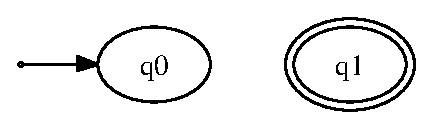
\epsfig{file=Abbildungen/aLeer.eps, scale=0.5}
      \caption{Der Automat $A(\emptyset)$.}
      \label{fig:aLeer.eps}
      \end{figure}
      Abbildung \ref{fig:aLeer.eps} zeigt den Automaten, der die durch $\emptyset$
      spezifizierte Sprache akzeptiert.  Der Automat besteht
      nur aus dem Start-Zustand $q_0$ und dem akzeptierenden Zustand $q_1$.
      Die Funktion $\delta$ liefert f�r alle Argumente die leere Menge, der Automat hat
      also keinerlei Zustands-�berg�nge und 
      akzeptiert daher nur die leere Sprache.  Damit gilt  $L(\emptyset) = \{\}$. 
\item Den Automaten $A(\varepsilon)$ definieren wir als
      \\[0.2cm]
      \hspace*{1.3cm}
      $A(\varepsilon) = \langle \{ q_0, q_1 \}, \Sigma, \{ \pair(q_0, \varepsilon) \mapsto q_1 \}, q_0, \{ q_1 \} \rangle$


      \begin{figure}[!ht]
        \centering
      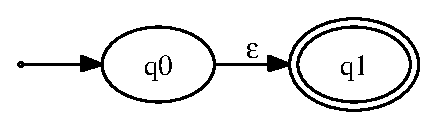
\epsfig{file=Abbildungen/aEpsilon.eps, scale=0.5}
      \caption{Der Automat $A(\varepsilon)$.}
      \label{fig:aEpsilon.eps}
      \end{figure}
      Abbildung \ref{fig:aEpsilon.eps} zeigt den Automaten, der die durch $\varepsilon$
      spezifizierte Sprache akzeptiert.  Der Automat besteht
      nur aus dem Start-Zustand $q_0$ und dem akzeptierenden Zustand $q_1$.
      Von dem Zustand $q_0$ gibt es eine $\varepsilon$-Transition zu dem Zustand $q_1$.
      Damit akzeptiert der Automat das leere Wort und sonst nichts. 
\item F�r einen Buchstaben $c \in \Sigma$ definieren wir den Automaten $A(c)$ durch
      \\[0.2cm]
      \hspace*{1.3cm}
      $A(c) = \langle \{ q_0, q_1 \}, \Sigma, 
                                \{ \langle q_0, c \rangle \mapsto q_1\}, q_0, \{ q_1 \} \rangle$

      \begin{figure}[!ht]
        \centering
      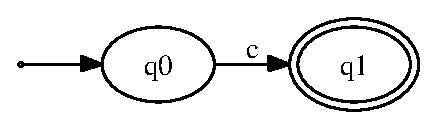
\epsfig{file=Abbildungen/aChar.eps, scale=0.5}
      \caption{Der Automat $A(c)$.}
      \label{fig:aChar.eps}
      \end{figure}
      Abbildung \ref{fig:aChar.eps} zeigt den Automaten, der die durch den Buchstaben $c$
      spezifizierte Sprache akzeptiert.  Der Automat besteht
      aus dem Start-Zustand $q_0$ und dem akzeptierenden Zustand $q_1$.
      Von dem Zustand $q_0$ gibt es eine Transition zu dem Zustand $q_1$, die beim Lesen
      des Buchstabens $c$ benutzt wird.
      Damit akzeptiert der Automat das Wort, das nur aus dem Buchstaben $c$ besteht und
      sonst nichts.
\item Um den Automaten $A(r_1 \cdot r_2)$ f�r die Konkatenation $r_1 \cdot r_2$ definieren
      zu k�nnen, nehmen wir zun�chst an, dass die 
      Zu\-st�n\-de der Automaten $A(r_1)$ und $A(r_2)$ verschieden sind.  Dies k�nnen
      wir immer erreichen, indem wir die Zust�nde des Automaten $A(r_2)$ umbennen.
      Wir nehmen nun an, dass $A(r_1)$ und $A(r_2)$ die folgende Formen haben:
      \begin{enumerate}
      \item $A(r_1) = \langle Q_1, \Sigma, \delta_1, q_1, \{ q_2 \}\rangle$,
      \item $A(r_2) = \langle Q_2, \Sigma, \delta_2, q_3, \{ q_4 \}\rangle$,
      \item $Q_1 \cap Q_2 = \{\}$.
      \end{enumerate}
      Damit k�nnen wir den endlichen Automaten $A(r_1 \cdot r_2)$ aus den beiden Automaten $A(r_1)$ und
      $A(r_2)$ zusammenbauen:  Dieser Automat ist gegeben durch
      \\[0.2cm]
      \hspace*{0.8cm}
       $\langle Q_1 \cup Q_2, \Sigma, 
                \{ \pair(q_2,\varepsilon) \mapsto q_3 \} 
                   \cup \delta_1 \cup \delta_2, q_0, \{ q_4 \} \rangle$
      \\[0.2cm]
      Die Notation $\{ \pair(q_2,\varepsilon) \mapsto q_3 \} \cup \delta_1 \cup \delta_2$
      ist so zu verstehen, dass die so spezifizierte Funktion $\delta$ alle �berg�nge
      enth�lt, die durch die Zustands-�bergangs-Funktionen $\delta_1$ und $\delta_2$
      spezifiziert sind.  Dazu kommt dann noch der $\varepsilon$-�bergang von $q_2$ nach
      $q_3$.  Formal k�nnten wir daher die Funktion $\delta$ auch wie folgt spezifizieren:
      \\[0.2cm]
      \hspace*{1.3cm}
      $\delta(q,c) := \left\{
      \begin{array}{ll}
        \{ q_3 \}       & \mbox{falls $q = q_2$ und $c = \varepsilon$}, \\[0.2cm]
        \delta_1(q, c)  & \mbox{falls $q \in Q_1$ und $\pair(q,c) \not= \pair(q_2,\varepsilon)$}, \\[0.2cm]
        \delta_2(q, c)  & \mbox{falls $q \in Q_2$.} 
      \end{array}\right.
      $
      \\[0.2cm]


      \begin{figure}[!ht]
        \centering
      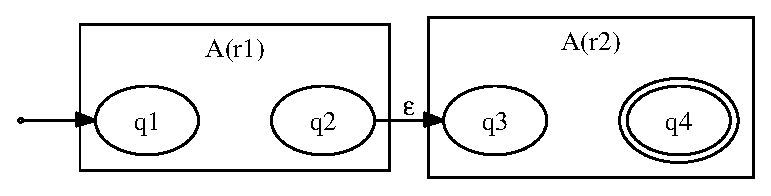
\epsfig{file=Abbildungen/aConcat.eps, scale=0.8}
      \caption{Der Automat $A(r_1 \cdot r_2)$.}
      \label{fig:aConcat.eps}
      \end{figure}
      Abbildung \ref{fig:aConcat.eps} zeigt den Automaten $A(r_1 \cdot r_2)$.

      Statt der $\varepsilon$-Transition von $q_2$ nach $q_3$ k�nnen wir die beiden
      Zust�nde $q_2$ und $q_3$ auch identifizieren.  Das hat den Vorteil, dass der
      resultierende Autmat dann etwas kleiner wird.  Bei den praktischen �bungen werden
      wir diese Zust�nde daher identifizieren.
\item Um den Automaten $A(r_1 + r_2)$ definieren zu k�nnen, nehmen wir wieder an, dass die
      Zust�nde der Automaten $A(r_1)$ und $A(r_2)$ verschieden sind.  
      Wir nehmen weiter an, dass $A(r_1)$ und $A(r_2)$ die folgende Formen haben:
      \begin{enumerate}
      \item $A(r_1) = \langle Q_1, \Sigma, \delta_1, q_1, \{ q_3 \}\rangle$,
      \item $A(r_2) = \langle Q_2, \Sigma, \delta_2, q_2, \{ q_4 \}\rangle$,
      \item $Q_1 \cap Q_2 = \{\}$.
      \end{enumerate}
      Damit k�nnen wir den Automaten $A(r_1 + r_2)$ aus den beiden Automaten $A(r_1)$ und
      $A(r_2)$ zusammenbauen:  Dieser Automat ist gegeben durch
      \\[0.2cm]
      \hspace*{0.8cm}
       $\langle \{ q_0, q_5 \} \cup Q_1 \cup Q_2, \Sigma, 
                \{ \pair(q_0,\varepsilon) \mapsto q_1, \pair(q_0,\varepsilon) \mapsto q_2,
                   \pair(q_3,\varepsilon) \mapsto q_5, \pair(q_4,\varepsilon) \mapsto q_5 \} 
                   \cup \delta_1 \cup \delta_2, q_0, \{ q_5 \} \rangle$

      \begin{figure}[!ht]
        \centering
      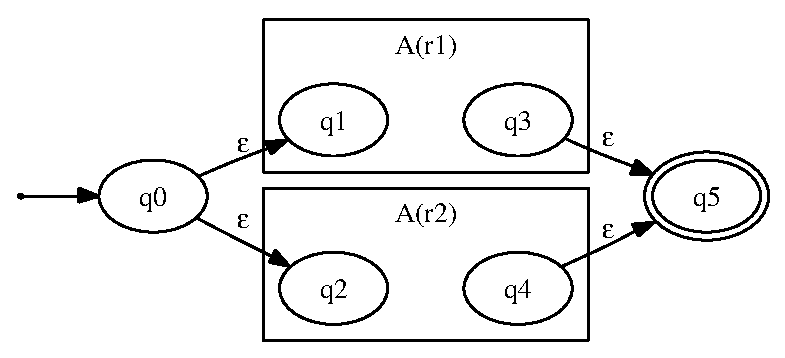
\epsfig{file=Abbildungen/aPlus.eps, scale=0.5}
      \caption{Der Automat $A(r_1 + r_2)$.}
      \label{fig:aPlus.eps}
      \end{figure}
      Abbildung \ref{fig:aPlus.eps} zeigt den Automaten $A(r_1 + r_2)$.
      Wir sehen, dass zus�tzlich zu den Zust�nden der beiden Automaten $A(r_1)$ und 
      $A(r_2)$ noch zwei weitere Zust�nde hinzukommen:
      \begin{enumerate}
      \item $q_0$ ist der Start-Zustand des Automaten $A(r_1 + r_2)$,
      \item $q_5$ ist der einzige akzeptierende Zustand des Automaten $A(r_1 + r_2)$.
      \end{enumerate}
      Gegen�ber den Zustands-�berg�nge der Automaten $A(r_1)$ und $A(r_2)$ kommen noch
      vier $\varepsilon$-Transitionen hinzu: 
      \begin{enumerate}
      \item Von dem neuen Start-Zustand $q_0$ gibt es jeweils eine
            $\varepsilon$-Transition zu den Start-Zust�nden $q_1$ und $q_2$ der Automaten
             $A(r_1)$ und $A(r_2)$.
      \item Von den akzeptierenden Zust�nden $q_3$ und $q_4$ der Automaten
             $A(r_1)$ und $A(r_2)$ gibt es jeweils eine $\varepsilon$-Transition zu dem
             akzeptierenden Zustand $q_5$.
      \end{enumerate}
      Um den so definierten Automaten zu vereinfachen, k�nnen wir einerseits die drei
      Zust�nde $q_0$, $q_1$ und $q_2$ und andererseits die drei Zust�nde 
      $q_3$, $q_4$ und $q_5$ identifizieren.
\item Um den Automaten $A(r^*)$ f�r den Kleene-Abschluss $r^*$ 
      definieren zu k�nnen, schreiben wir $A(r)$ als
      \\[0.2cm]
      \hspace*{1.3cm}
      $A(r) = \langle Q, \Sigma, \delta, q_1, \{ q_2 \} \rangle$,
      \\[0.2cm]
      Damit k�nnen wir  $A(r^*)$ aus dem Automaten $A(r)$ 
      konstruieren:  Der Automat $A(r^*)$ ist  durch den Ausdruck
      \\[0.2cm]
      \hspace*{0.8cm}
       $\langle \{ q_0, q_3 \} \cup Q, \Sigma, 
                \{ \pair(q_0,\varepsilon) \mapsto q_1, \pair(q_2,\varepsilon) \mapsto q_1,
                   \pair(q_0,\varepsilon) \mapsto q_3, \pair(q_2,\varepsilon) \mapsto q_3 \} 
                   \cup \delta, q_0, \{ q_3 \} \rangle$
      \\[0.2cm]
      gegeben.

      \begin{figure}[!ht]
        \centering
      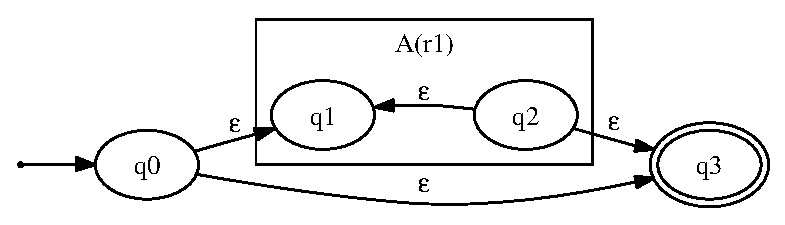
\epsfig{file=Abbildungen/aStar.eps, scale=0.5}
      \caption{Der Automat $A(r^*)$.}
      \label{fig:aStar.eps}
      \end{figure}
      Abbildung \ref{fig:aStar.eps} zeigt den Automaten $A(r^*)$.
      Wir sehen, dass zus�tzlich zu den Zust�nden des  Automaten $A(r)$ 
      noch zwei weitere Zust�nde hinzukommen:
      \begin{enumerate}
      \item $q_0$ ist der Start-Zustand des Automaten $A(r^*)$,
      \item $q_3$ ist der einzige akzeptierende Zustand des Automaten $A(r^*)$.
      \end{enumerate}
      Zu den Zustands-�berg�nge des Automaten $A(r)$  kommen 
      vier $\varepsilon$-Transitionen hinzu: 
      \begin{enumerate}
      \item Von dem neuen Start-Zustand $q_0$ gibt es jeweils eine
            $\varepsilon$-Transition zu den Zust�nden $q_1$ und $q_3$.
      \item Von $q_2$ gibt es eine  $\varepsilon$-Transition zur�ck zu dem
            Zustand $q_1$.
      \item Von $q_2$ gibt es eine  $\varepsilon$-Transition zu dem
            Zustand $q_3$.
      \end{enumerate}
      \textbf{Achtung}:  Wenn wir bei diesem Automaten versuchen w�rden, die Zust�nde
      $q_0$ und $q_1$ bzw.~$q_2$ und $q_3$ zu identifizieren, dann funktioniert das in 
      diesem Abschnitt beschriebene Verfahren in bestimmten  F�llen nicht mehr.  Diese
      Zust�nde d�rfen also \textbf{nicht} identifiziert werden!
\end{enumerate}

\exercise
Konstruieren Sie einen nicht-deterministischen endlichen Automaten, der die durch
den regul�ren Ausdruck
\\[0.2cm]
\hspace*{1.3cm}
$(\texttt{a} + \texttt{b}) \cdot \texttt{a}^* \cdot \texttt{b}$
\\[0.2cm]
spezifizierte Sprache erkennt.

\exercise
Konstruieren Sie einen nicht-deterministischen endlichen Automaten, der die durch
den regul�ren Ausdruck
\\[0.2cm]
\hspace*{1.3cm}
$\texttt{a}^* \cdot \texttt{b}^*$
\\[0.2cm]
spezifizierte Sprache erkennt.  �berlegen Sie sich, warum Sie in diesem Beispiel bei der Konstruktion zur
Berechnung des Kleene-Abschlusses die Zust�nde, die in dem im Text beschriebenen
Algorithmus die Namen $q_0$ und $q_1$ bzw.~$q_2$ und $q_3$ haben, nicht identifizieren
d�rfen.

\subsection{Implementing the Conversion of Regular Expressions into \textsc{Fsm}s}
In this section, we develop a \textsc{SetlX} program that transforms a regular expression
into a non-deterministic finite state machine.  In order to do so, we first have to decide
how to represent regular expressions.  It is convenient to represent complex regular expressions as
terms.  In \textsc{SetlX}, a term has the form
\\[0.2cm]
\hspace*{1.3cm}
$F(t_1, \cdots, t_N)$.
\\[0.2cm]
Here, $F$ needs to be a \emph{functor}, which is just an uninterpreted function symbols.
In \textsc{SetlX}, functors have to start with a capital letter.  The arguments $t_1$,
$\cdots$, $t_n$ are either terms, strings, numbers, sets, or lists.  In general, we define a function
\\[0.2cm]
\hspace*{1.3cm}
$\textsl{rep}: \textsl{RegExp} \rightarrow \textsc{SetlX}$
\\[0.2cm]
that maps a regular expression $r$ into a value of the programming language
\textsc{SetlX}.  The idea is that for a given regular expression $r$, $\textsl{rep}(r)$ is
the \textsc{SetlX} term that represents the regular expression $r$.  
We define $\textsl{rep}(r)$ by induction on the definition of the regular
expression $r$.
\begin{enumerate}
\item $\textsl{rep}(\emptyset) := \texttt{0}$.

      The regular expression $\emptyset$ is represented as the number \texttt{0}.
\item $\textsl{rep}(\varepsilon) := \texttt{\symbol{34}\symbol{34}}$.
  
      The regular expression $\varepsilon$ is represented as the empty string.
\item $\textsl{rep}(c) := \texttt{\symbol{34}$c$\symbol{34}}$.

      A single character $c$ is represented by the string containing just this character.
\item $\textsl{rep}(r_1 \cdot r_2) := \texttt{Cat($\textsl{rep}(r_1)$, $\textsl{rep}(r_2)$)}$.
  
      The concatenation $r_1 \cdot r_2$ of two regular expressions $r_1$ and $r_2$ is
      represented by a term with the functor ``\texttt{Cat}'', while the arguments of this
      functor are the representations of the regular expressions $r_1$ and $r_2$.
\item $\textsl{rep}(r_1 + r_2) := \texttt{Or($r_1$, $r_2$)}$.

      The disjunction $r_1 + r_2$ of two regular expressions $r_1$ and $r_2$ is
      represented by a term with the functor ``\texttt{Or}''.

\item $\textsl{rep}(r^*) := \texttt{Star($\textsl{rep}(r))$}$.

      The Kleene closure $r^*$ of the  regular expression $r$ is
      represented by a term with the functor ``\texttt{Star}''.
\end{enumerate}


\begin{figure}[!ht]
\centering
\begin{Verbatim}[ frame         = lines, 
                  framesep      = 0.3cm, 
                  firstnumber   = 1,
                  labelposition = bottomline,
                  numbers       = left,
                  numbersep     = -0.2cm,
                  xleftmargin   = 0.8cm,
                  xrightmargin  = 0.8cm,
                ]
    class regexp2NFA(sigma) {
        this.gStateCount := -1;
        this.mSigma      := sigma;
        
        toNFA         := procedure(r)      { ... };    
        genEmptyNFA   := procedure()       { ... };
        genEpsilonNFA := procedure()       { ... };
        genCharNFA    := procedure(c)      { ... };
        catenate      := procedure(f1, f2) { ... };
        disjunction   := procedure(f1, f2) { ... };
        kleene        := procedure(f)      { ... };
        getNewState   := procedure()       { ... };
    }
\end{Verbatim}
\vspace*{-0.3cm}
\caption{Outline of the class \texttt{regexp2NFA}}
\label{fig:regexp-2-nfa.stlx}
\end{figure}

\noindent
We proceed to discuss the implementation of a program transforming a regular expression into a
non-deterministic finite state machine.
Figure \ref{fig:regexp-2-nfa.stlx} on page \pageref{fig:regexp-2-nfa.stlx} shows the outline of the
class \texttt{regexp2NFA} that serves as this implementation.  
\begin{enumerate}
\item The class has two member variables.
      \begin{enumerate}
      \item \texttt{gStateCount} is a counter that is used to number the states of the finites state
            machine.
      \item \texttt{mSigma} is the alphabet.
      \end{enumerate}
\item $\texttt{toNFA}(r)$ is a method that takes a regular expression $r$ and transforms this regular
      expression into a non-deterministic finite state machine that recognizes the language
      specified by $r$.
\item \texttt{genEmptyNFA} generates a non-deterministic \textsc{Fsm} that recognizes the empty language. 
\item \texttt{genEpsilonNFA} generates a non-deterministic \textsc{Fsm} that recognizes the language
      containing only the empty string. 
\item $\texttt{genCharNFA}(c)$ takes a character $c$ as argument and generates a non-deterministic \textsc{Fsm} that recognizes the
      language $L = \{ c \}$.
\item $\texttt{catenate}(f_1, f_2)$ takes two non-deterministic \textsc{Fsm}s $f_1$ and $f_2$ as arguments and
      generates a non-deterministic \textsc{Fsm} that recognizes the language $L(f_1) \cdot L(f_2)$.
      Here, $L(f_1)$ is the language recognized by $f_1$ and similarly $L(f_2)$ is the language
      recognized by $f_2$.
\item $\texttt{disjunction}(f_1, f_2)$ takes two non-deterministic \textsc{Fsm}s $f_1$ and $f_2$ as arguments and
      generates a non-deterministic \textsc{Fsm} that recognizes the language $L(f_1) \cup L(f_2)$.
\item $\texttt{kleene}(f)$ takes a non-deterministic \textsc{Fsm}s $f$ as argument and
      generates a non-deterministic \textsc{Fsm} that recognizes the language $\bigl(L(f)\bigr)^*$.
\item \texttt{getNewState} is an auxiliary function that increments the global variable \texttt{gStateCount} and returns a name
      for the corresponding state.
\end{enumerate}
We proceed to discuss the implementations of methods of the class \texttt{regexp2NFA} in detail.


\begin{figure}[!ht]
\centering
\begin{Verbatim}[ frame         = lines, 
                  framesep      = 0.3cm, 
                  firstnumber   = 1,
                  labelposition = bottomline,
                  numbers       = left,
                  numbersep     = -0.2cm,
                  xleftmargin   = 0.8cm,
                  xrightmargin  = 0.8cm,
                ]
    toNFA := procedure(r) {
        match (r) {
            case 0 : return genEmptyNFA();
            case "": return genEpsilonNFA();
            case c | isString(c) && #c == 1: 
                 return genCharNFA(c);
            case Cat(r1, r2): 
                 return catenate(toNFA(r1), toNFA(r2));
            case Or(r1, r2): 
                 return disjunction(toNFA(r1), toNFA(r2));
            case Star(r0): 
                 return kleene(toNFA(r0));
            default: abort("$r$ is not a suitable regular expression");
        }
    };    
\end{Verbatim} 
\vspace*{-0.3cm}
\caption{Converting a regular expression into a non-deterministic finite state machine.}
\label{fig:regexp-2-nfa.stlx:toNFA}
\end{figure}
%$


The implementation of the function \texttt{regexp2NFA} is shown in
Figure \ref{fig:regexp-2-nfa.stlx:toNFA} on page \pageref{fig:regexp-2-nfa.stlx:toNFA}.
The function \texttt{toNFA} takes a regular expression $r$ as its argument.  
The implementation branches in line 2 on the form of the regular
expression $r$.  Altogether, there are six different cases.
\begin{enumerate}
\item If $r= \texttt{0}$, then $r$ represents the regular expression  $\emptyset$.
      In this case, the function \texttt{genEmptyNFA} computes the finite state machine that
      is shown in Figure \ref{fig:aLeer.eps}.  
      
      The implementation of the function \texttt{genEmptyNFA} is shown in Figure
      \ref{fig:regexp-2-nfa.stlx:genEmptyNFA} on page \pageref{fig:regexp-2-nfa.stlx:genEmptyNFA}:
      First, we generate two new states \texttt{q0} and \texttt{q1}.  The transition function
      \texttt{delta} is defined in line 4 as the function mapping every pair $\pair(q,c)$ to the
      empty set.  Finally, line 5 returns the 5-tuple
      \\[0.2cm]
      \hspace*{1.3cm}
      $\langle \{\texttt{q0}, \texttt{q1}\}, \Sigma, \delta, \texttt{q0}, \{\texttt{q1}\}\rangle$
      \\[0.2cm]
      as the result.  This corresponds one-to-one with the finite state machine shown in Figure
      \ref{fig:aLeer.eps}.

\begin{figure}[!ht]
\centering
\begin{Verbatim}[ frame         = lines, 
                  framesep      = 0.3cm, 
                  firstnumber   = 1,
                  labelposition = bottomline,
                  numbers       = left,
                  numbersep     = -0.2cm,
                  xleftmargin   = 0.8cm,
                  xrightmargin  = 0.8cm,
                ]
    genEmptyNFA := procedure(sigma) {
        q0 := getNewState();
        q1 := getNewState();
        delta := [q, c] |-> {};
        return [ {q0, q1}, sigma, delta, q0, { q1 } ];
    };
\end{Verbatim}
\vspace*{-0.3cm}
\caption{Generating the NFA shown in Figure \ref{fig:aLeer.eps}.}
\label{fig:regexp-2-nfa.stlx:genEmptyNFA}
\end{figure}

\item If $r = \texttt{\symbol{34}\symbol{34}}$, then $r$ represents the regular expression
      $\varepsilon$.  In this case, the function \texttt{genEpsilonNFA} computes the finite state
      machine that is shown in Figure \ref{fig:aEpsilon.eps}.

      The implementation of the function \texttt{genEpsilonNFA} is shown in Figure
      \ref{fig:regexp-2-nfa.stlx:genEpsilonNFA} on page \pageref{fig:regexp-2-nfa.stlx:genEpsilonNFA}:
      First, we generate two new states \texttt{q0} and \texttt{q1}.  The transition function
      \texttt{delta} is then defined in lines 4 -- 10.  There is exactly one
      $\varepsilon$-transition from the state $\mathtt{q0}$ to the state $\mathtt{q1}$.
      

      
\begin{figure}[!ht]
\centering
\begin{Verbatim}[ frame         = lines, 
                  framesep      = 0.3cm, 
                  firstnumber   = 1,
                  labelposition = bottomline,
                  numbers       = left,
                  numbersep     = -0.2cm,
                  xleftmargin   = 0.8cm,
                  xrightmargin  = 0.8cm,
                ]
     genEpsilonNFA := procedure() {
        q0 := getNewState();
        q1 := getNewState();
        delta := procedure(q, c) { 
                     if (q == q0 && c == "") { 
                         return { q1 };
                     } else { 
                         return {};
                     }
                 };
        return [ {q0, q1}, mSigma, delta, q0, { q1 } ];
    };
\end{Verbatim}
\vspace*{-0.3cm}
\caption{Generating the NFA shown in Figure \ref{fig:aEpsilon.eps}.}
\label{fig:regexp-2-nfa.stlx:genEpsilonNFA}
\end{figure}

\item If $r = \texttt{\symbol{34}}c\texttt{\symbol{34}}$, then $r$ represents a single character $c$.
      In this case, the function \texttt{genCharNFA} computes the finite state
      machine that is shown in Figure \ref{fig:aChar.eps}.

      The implementation of the function \texttt{genCharNFA} is shown in Figure
      \ref{fig:regexp-2-nfa.stlx:genCharNFA} on page \pageref{fig:regexp-2-nfa.stlx:genCharNFA}:
      After generating  two new states \texttt{q0} and \texttt{q1},   the transition function
      \texttt{delta} is defined in lines 4--10.



\begin{figure}[!ht]
\centering
\begin{Verbatim}[ frame         = lines, 
                  framesep      = 0.3cm, 
                  firstnumber   = 1,
                  labelposition = bottomline,
                  numbers       = left,
                  numbersep     = -0.2cm,
                  xleftmargin   = 0.8cm,
                  xrightmargin  = 0.8cm,
                ]
    genCharNFA := procedure(c) {
        q0 := getNewState();
        q1 := getNewState();
        delta := procedure(q, d) { 
                      if (q == q0 && d == c) { 
                          return { q1 };
                      } else { 
                          return {};
                      }
                  };
        return [ {q0, q1}, mSigma, delta, q0, { q1 } ];
    };
\end{Verbatim}
\vspace*{-0.3cm}
\caption{Generating the NFA shown in Figure \ref{fig:aChar.eps}.}
\label{fig:regexp-2-nfa.stlx:genCharNFA}
\end{figure}

\item If $r = \texttt{Cat}(r_1,r_2)$, then $r$ represents the concatenation $r_1 \cdot r_2$ of the regular
      expressions $r_1$ and $r_2$. In this case,  we recursively compute two 
      finite state machines
      that recognize the strings corresponding to these regular expressions.
      These two finite state machines are then combined into a
      new finite state machine using the function \texttt{catenate}.  The function \texttt{catenate}
      works as specified in Figure \ref{fig:aConcat.eps}.

      The implementation of the function \texttt{catenate} is shown in Figure
      \ref{fig:regexp-2-nfa.stlx:catenate} on page \pageref{fig:regexp-2-nfa.stlx:catenate}:
      The function \texttt{catenate} receives two finite state machines \texttt{f1} and \texttt{f2}
      as arguments.  These finite state machines are split into their components in line 2 and line
      3.   The function $\texttt{arb}(s)$ extracts an arbitrary element from the set $s$.  
      This function is called in line 4 and 5 to extract the accepting states \texttt{q2} and
      \texttt{q4} of the finite state machines \texttt{f1} and \texttt{f2}.  This works since we
      know that the sets of accepting states \texttt{f1} and \texttt{f2} contain exactly one state
      each, so the function \texttt{arb} doesn't really have a choice which state to pick.  
      
      The most important purpose of the function \texttt{catenate} is to construct a new transition 
      function $\delta$ such that 
      \\[0.2cm]
      \hspace*{1.3cm}
      $\delta = \delta_1 \cup \delta_2 \cup \{ \pair(q_2, \varepsilon) \mapsto \{ q_3 \} \}$
      \\[0.2cm]
      holds.  This function is defined in lines 6 -- 16.


\begin{figure}[!ht]
\centering
\begin{Verbatim}[ frame         = lines, 
                  framesep      = 0.3cm, 
                  firstnumber   = 1,
                  labelposition = bottomline,
                  numbers       = left,
                  numbersep     = -0.2cm,
                  xleftmargin   = 0.8cm,
                  xrightmargin  = 0.8cm,
                ]
    catenate := procedure(f1, f2) {
        [m1, _, delta1, q1, a1] := f1;
        [m2, _, delta2, q3, a2] := f2;
        q2 := arb(a1);
        q4 := arb(a2);
        delta := procedure(q, c) {
                     if (q == q2 && c == "") {
                         return { q3 };
                     } else if (q in m1) {
                         return delta1(q, c);
                     } else if (q in m2) {
                         return delta2(q, c);
                     } else {
                         return {};
                     }
                 };
        return [ m1 + m2, mSigma, delta, q1, a2 ];
    };
\end{Verbatim}
\vspace*{-0.3cm}
\caption{Generating the NFA shown in Figure \ref{fig:aConcat.eps}.}
\label{fig:regexp-2-nfa.stlx:catenate}
\end{figure}

\item The remaining two cases correspond to the diagrams shown in Figure \ref{fig:aPlus.eps} and
      Figure \ref{fig:aStar.eps}.  As these cases are quite similar to the last case, there is
      no need for a detailed discussion.

\begin{figure}[!ht]
\centering
\begin{Verbatim}[ frame         = lines, 
                  framesep      = 0.3cm, 
                  firstnumber   = 1,
                  labelposition = bottomline,
                  numbers       = left,
                  numbersep     = -0.2cm,
                  xleftmargin   = 0.8cm,
                  xrightmargin  = 0.8cm,
                ]
    disjunction := procedure(f1, f2) {
        [m1, _, delta1, q1, a1] := f1;
        [m2, _, delta2, q2, a2] := f2;
        q3 := arb(a1);
        q4 := arb(a2);
        q0 := getNewState(); 
        q5 := getNewState(); 
        delta := procedure(q, c) {
                     if (q == q0 && c == "") {
                         return { q1, q2 };
                     } else if (q in { q3, q4 } && c == "") {
                         return { q5 };
                     } else if (q in m1) {
                         return delta1(q, c);
                     } else if (q in m2) {
                         return delta2(q, c);
                     } else {
                         return {};
                     } 
                 };
        return [ { q0, q5 } + m1 + m2, mSigma, delta, q0, { q5 } ];
    };
\end{Verbatim}
\vspace*{-0.3cm}
\caption{Generating the NFA shown in Figure \ref{fig:aPlus.eps}.}
\label{fig:regexp-2-nfa.stlx:disjunction}
\end{figure}

\begin{figure}[!ht]
\centering
\begin{Verbatim}[ frame         = lines, 
                  framesep      = 0.3cm, 
                  firstnumber   = 1,
                  labelposition = bottomline,
                  numbers       = left,
                  numbersep     = -0.2cm,
                  xleftmargin   = 0.8cm,
                  xrightmargin  = 0.8cm,
                ]
    kleene := procedure(f) {
        [m, _, delta0, q1, a] := f;
        q2 := arb(a);
        q0 := getNewState(); 
        q3 := getNewState(); 
        delta := procedure(q, c) {
                     if (q == q0 && c == "") {
                         return { q1, q3 };
                     } else if (q == q2 && c == "") {
                         return { q1, q3 };
                     } else if (q in m) {
                         return delta0(q, c);
                     } else {
                         return {};
                     } 
                 };
        return [ { q0, q3 } + m, mSigma, delta, q0, { q3 } ];
    };
\end{Verbatim}
\vspace*{-0.3cm}
\caption{Generating the NFA shown in Figure \ref{fig:aStar.eps}.}
\label{fig:regexp-2-nfa.stlx:kleene}
\end{figure}
\end{enumerate}


\begin{figure}[!ht]
\centering
\begin{Verbatim}[ frame         = lines, 
                  framesep      = 0.3cm, 
                  firstnumber   = 1,
                  labelposition = bottomline,
                  numbers       = left,
                  numbersep     = -0.2cm,
                  xleftmargin   = 0.8cm,
                  xrightmargin  = 0.8cm,
                ]
    getNewState := procedure() {
        gStateCount += 1;
        return "q" + gStateCount;
    };
\end{Verbatim}
\vspace*{-0.3cm}
\caption{Generating a new state.}
\label{fig:regexp-2-nfa.stlx:getNewState}
\end{figure}

\pagebreak
\vspace*{\fill}

\pagebreak



\section{�bersetzung eines \textsc{EA} in einen regul�ren Ausdruck}
Wir runden die Theorie ab indem wir zeigen, dass sich zu jedem deterministischen endlichen
Automaten $A$ ein regul�rer Ausdruck $r(A)$ angeben l�sst, der dieselbe Sprache spezifiziert,
die von dem Automaten $A$ akzeptiert wird, f�r den also
\\[0.2cm]
\hspace*{1.3cm}
$L\bigl(r(A)\bigr) = L(A)$
\\[0.2cm]
gilt.  Der  Automat $A$ habe die Form
\\[0.2cm]
\hspace*{1.3cm}
$A = \langle \{ q_0, q_1, \cdots, q_n \}, \Sigma, \delta, q_0, F \rangle$.
\\[0.2cm]
F�r jedes Paar von Zust�nden $\pair(p_1,p_2) \in Q \times Q$ definieren wir einen regul�ren Ausdruck
$r(p_1, p_2)$.   Die Idee bei dieser Definition ist, dass der regul�re Ausdruck
$r(p_1, p_2)$ alle die Strings $w$ spezifiziert, die den Automaten $A$ von dem Zustand
$p_1$ in den Zustand $p_2$ �berf�hren, formal gilt:
\\[0.2cm]
\hspace*{1.3cm}
$L\bigl(r(p_1, p_2)\bigr) = 
  \bigl\{ w \in \Sigma^* \mid \pair(p_1,w) \leadsto^* \pair(p_2, \varepsilon) \bigr\}$
\\[0.2cm]  
Die Definition der regul�ren Ausdr�cke erfolgt �ber einen Trick: Wir definieren f�r
$k=0,\cdots,n+1$ regul�re Ausdr�cke $r^{(k)}(p_1, p_2)$.   Der regul�re Ausdruck
beschreibt gerade die Strings, die den Automaten $A$ von dem Zustand
$p_1$ in den Zustand $p_2$ �berf�hren, \underline{ohne} dass dabei zwischendurch ein
Zustand aus der Menge 
\\[0.2cm]
\hspace*{1.3cm}
$Q_k := \bigl\{ q_i \mid i \in \{k,\cdots,n \}  \bigl\} = \{ q_k, \cdots, q_n \}$ 
\\[0.2cm]
besucht wird.  Die Menge $Q_k$ enth�lt also nur die Zust�nde, deren Index gr��er oder
gleich $k$ ist.
Formal definieren wir dazu die dreistellige Relation 
\\[0.2cm]
\hspace*{1.3cm}
$\mapsto_k \;\subseteq\; (Q \times \Sigma^* \times Q)$.
\\[0.2cm]
F�r zwei Zust�nde $p, q \in Q$ und einen String $w$ soll 
\\[0.2cm]
\hspace*{1.3cm}
$p \stackrel{w}{\mapsto}_k q$
\\[0.2cm]
genau dann gelten, wenn der Automat $A$ von dem Zustand $p$ beim Lesen des Wortes $w$ in
den Zustand $q$ �bergeht, ohne dabei \underline{zwischendurch} in einen Zustand aus der
Menge $Q_k$ zu wechseln.  Mit ``zwischendurch'' ist hier gemeint, dass die Zust�nde $p$
und $q$ sehr wohl in der Menge $Q_k$ liegen k�nnen.  Die formale Definition der Relation 
$p \stackrel{w}{\mapsto}_k q$ erfolgt durch Induktion nach der L�nge des Wortes $w$:
\begin{enumerate}
\item[I.A.:] $|w| \leq 1$.  Im Induktions-Anfang haben wir zwei F�lle:
  \begin{enumerate}
  \item $p \stackrel{\varepsilon}{\mapsto}_k p$,

        denn mit dem leeren Wort kann von $p$ aus nur der Zustand $p$ erreicht
        werden.
  \item $\delta(p, c) = q \;\Rightarrow\; p \stackrel{c}{\mapsto}_k q$,

        denn wenn der Automat beim Lesen des Buchstabens $c$ von dem Zustand $p$ direkt
        in den Zustand $q$ �bergeht, dann werden zwischendurch keine Zust�nde aus $Q_k$
        besucht, denn es werden �berhaupt keine Zust�nde zwischendurch besucht.
  \end{enumerate}
\item[I.S.:] $w = cv$.

             \hspace*{1.3cm}
            $p \stackrel{c}{\mapsto} q \wedge q \not\in Q_k \wedge q \stackrel{v}{\mapsto}_k r
              \Rightarrow p \stackrel{cv}{\mapsto}_k r$.

             Wenn der Automat $A$ von dem Zustand $p$ durch Lesen des Buchstabens $c$
             in einen  Zustand $q \notin Q_k$ �bergeht und wenn der Automat dann von
             diesem Zustand $q$ beim Lesen von $v$ in den Zustand $r$ �bergehen kann, ohne
             dabei Zust�nde aus $Q_k$ zu benutzen, dann geht der Automat beim Lesen von
             $cv$ aus dem Zustand $p$ in den Zustand $r$ �ber,
             ohne zwischendurch in Zust�nde aus $Q_k$ zu wechseln.
\end{enumerate}
Damit k�nnen wir nun f�r alle $k=0,\cdots,n+1$ die regul�ren Ausdr�cke
$r^{(k)}(p_1, p_2)$ definieren.  Wir werden diese regul�ren Ausdr�cke so definieren, dass
hinterher
\\[0.2cm]
\hspace*{1.3cm}
$L\bigl(r^{(k)}(p_1, p_2)\bigr) = \bigl\{ w \in \Sigma^* \mid p_1 \stackrel{w}{\mapsto}_k p_2 \bigr\}$
\\[0.2cm]
gilt.
Die Definition der regul�ren Ausdr�cke $r^{(k)}(p_1, p_2)$ erfolgt durch eine Induktion nach $k$.
\begin{enumerate}
\item[I.A.:] $k = 0$.  

  Dann gilt $Q_0 = Q$, die Menge $Q_0$ enth�lt also alle Zust�nde
  und damit d�rfen wir, wenn wir vom Zustand $p_1$ in den Zustand $p_2$ �bergehen,
  zwischendurch �berhaupt keine Zust�nde besuchen.

  Wir betrachten zun�chst den Fall $p_1 \not= p_2$.  Dann kann $p_1 \stackrel{w}{\mapsto}_0 p_2$ nur dann gelten, wenn $w$ aus einem
  einzigen Buchstaben besteht.   Es sei
  \\[0.2cm]
  \hspace*{1.3cm}
  $\{ c_1, \cdots, c_l \} := \{ c \in \Sigma \mid \delta(p_1,c) = p_2 \}$
  \\[0.2cm]
  die Menge aller Buchstaben, die den Zustand $p_1$ in den Zustand $p_2$ �berf�hren.
  Falls diese Menge nicht leer ist, setzen wir 
  \\[0.2cm]
  \hspace*{1.3cm}
  $r^{(0)}(p_1, p_2) := c_1 + \cdots + c_l$. 
  \\[0.2cm]
  Ist die obige Menge leer, so gibt es keinen direkten �bergang von
  $p_1$ nach $p_2$ und wir setzen 
  \\[0.2cm]
  \hspace*{1.3cm}
  $r^{(0)}(p_1, p_2) := \emptyset$.

  Wir betrachten jetzt den Fall $p_1 = p_2$.  Definieren wir wieder
  \\[0.2cm]
  \hspace*{1.3cm}
  $\{ c_1, \cdots, c_l \} := \{ c \in \Sigma \mid \delta(p_1,c) = p_1 \}$
  \\[0.2cm]
  als die Menge aller Buchstaben, die den Zustand $p_1$ in sich selbst �berf�hren,
  so k�nnen wir in dem Fall, dass diese Menge nicht leer ist, 
  \\[0.2cm]
  \hspace*{1.3cm}
  $r^{(0)}(p_1, p_1) := c_1 + \cdots + c_l + \varepsilon$,
  \\[0.2cm]
  setzen.  Ist die obige Menge leer, so gibt es nur den �bergang mit dem leeren Wort
  von $p_1$ nach $p_1$ und wir setzen 
  \\[0.2cm]
  \hspace*{1.3cm}
  $r^{(0)}(p_1, p_1) := \varepsilon$.
\item[I.S.:] $k \mapsto k+1$.  

  Bei dem �bergang von $r^{(k)}(p_1, p_2)$ zu  $r^{(k+1)}(p_1, p_2)$ d�rfen wir zus�tzlich
  den Zustand $q_k$ benutzen, denn $q_k$ ist das einzige Element der Menge $Q_k$, das
  nicht in der Menge $q_{k+1}$ enthalten ist.  Wird ein String $w$ gelesen, der
  den Zustand $p_1$ in den Zustand $p_2$ �berf�hrt, ohne dabei zwischendurch in einen
  Zustand aus der Menge $Q_{k+1}$ zu wechseln, so gibt es zwei M�glichkeiten:
  \begin{enumerate}
  \item Es gilt bereits $p_1 \stackrel{w}{\mapsto}_k p_2$.
  \item Der String $w$ kann so in mehrere Teile $w_1 s_1\cdots s_l w_2$ aufgeteilt werden,
        dass gilt
        \begin{itemize}
        \item $p_1 \stackrel{w_1}{\mapsto}_k q_k$,

               von dem Zustand $p_1$ gelangt der Automat also beim Lesen von $w_1$
               zun�chst in den Zustand $q_k$, wobei zwischendurch der Zustand
               $q_k$ nicht benutzt wird.
        \item $q_k \stackrel{s_i}{\mapsto}_k q_k$ \quad f�r alle $i = \{ 1, \cdots, l\}$,

              von dem Zustand $q_k$ wechselt der Automat beim Lesen der Teilstrings
              $s_i$ wieder in den Zustand $q_k$.
        \item $q_k \stackrel{w_2}{\mapsto}_k p_2$,

              schlie�lich wechselt der Automat von dem Zustand $q_k$ in den Zustand
              $p_2$, wobei der Rest $w_2$ gelesen wird.
        \end{itemize}
        Daher definieren wir
        \\[0.2cm]
        \hspace*{1.3cm}
        $r^{(k+1)}(p_1,p_2) := 
         r^{(k)}(p_1,p_2) + 
         r^{(k)}(p_1,q_k) \cdot \bigl(r^{(k)}(q_k,q_k)\bigr)^* \cdot r^{(k)}(q_k,p_2)$.
        \\[0.2cm]
        Dieser Ausdruck kann wie folgt gelesen werden:  Um von $p_1$ nach $p_2$ zu kommen,
        ohne den Zustand $q_{k}$ zu benutzen, kann der Automat entweder direkt
        von $p_1$ nach $p_2$ gelangen, ohne $q_k$ zu benutzen, was dem Ausdruck 
        $r^{(k)}(p_1,p_2)$ entspricht, oder aber der Automat wechselt von $p_1$ ein erstes Mal
        in den Zustand $q_k$, was den Ausdruck $r^{(k)}(p_1,q_k)$ erkl�rt, wechselt dann beliebig oft
        von $q_k$ nach $q_k$,  was den Ausdruck  $\bigl(r^{(k)}(q_k,q_k)\bigr)^*$ erkl�rt und wechselt
        schlie�lich von $q_k$ in den Zustand $p_2$, wof�r der Ausdruck $r^{(k)}(q_k,p_2)$ steht. 
  \end{enumerate}  
\end{enumerate}
Nun haben wir alles Material zusammen, um die Ausdr�cke $r(p_1,p_2)$ definieren zu k�nnen.
Wir setzen 
\\[0.2cm]
\hspace*{1.3cm}
$r(p_1,p_2) := r^{(n+1)}(p_1,p_2)$. 
\\[0.2cm]
Dieser regul�re Ausdruck beschreibt die W�rter, die den Automaten von dem Zustand $p_1$ in
den Zustand $p_2$ �berf�hren, ohne dass der Automat dabei in einen Zustand der Menge
$Q_{n+1}$ wechselt.   Nun gilt aber
\\[0.2cm]
\hspace*{1.3cm}
$Q_{n+1} = \{ q_i | i \in \{0,\cdots,n \} \wedge i \geq n+1 \} = \{\}$,
\\[0.2cm]
die Menge ist also leer!  Folglich werden durch den regul�ren Ausdruck $r^{(n+1)}(p_1,p_2)$
�berhaupt keine Zust�nde ausgeschlossen:  Der Ausdruck beschreibt also genau die Strings,
die den Zustand $p_1$ in den Zustand $p_2$ �berf�hren, es gilt also
\\[0.2cm]
\hspace*{1.3cm}
$r^{(n+1)}(p_1,p_2) = r(p_1,p_2)$.
\\[0.2cm]
Um nun einen regul�ren Ausdruck konstruieren zu k�nnen, der die Sprache des Automaten $A$
beschreibt, schreiben wir die Menge $F$ der akzeptierenden Zust�nde von $A$ als
\\[0.2cm]
\hspace*{1.3cm}
$F = \{ t_1, \cdots, t_m \}$
\\[0.2cm]
und definieren den regul�ren Ausdruck $r(A)$ als
\\[0.2cm]
\hspace*{1.3cm}
$r(A) := r(q_0, t_1) + \cdots + r(q_0, t_m)$
\\[0.2cm]
definieren.  Dieser Ausdruck beschreibt genau die Strings, die den Automaten $A$ aus dem Start-Zustand
in einen der akzeptierenden Zust�nde �berf�hren.
\qed
\vspace*{0.3cm}


\noindent
Damit sehen wir jetzt, dass die Konzepte ``\emph{deterministischer endlicher Automat}'' und
``\emph{regul�rer Ausdruck}'' �quivalent sind.
\begin{enumerate}
\item Jeder deterministische endliche Automat kann in einen �quivalenten regul�ren
      Ausdruck �bersetzt werden.
\item Jeder regul�re Ausdruck kann in einen �quivalenten nicht-deterministischen endlichen Automaten
      transformiert werden.
\item Ein nicht-deterministischer endlicher Automat l�sst sich durch die
      Teilmengen-Konstruktion in einen endlichen Automaten �berf�hren.
\end{enumerate}

\exercise
Konstruieren Sie f�r den in Abbildung \ref{fig:abstara.dot} gezeigten endlichen Automaten einen
�quivalenten regul�ren Ausdruck.  


\solution
Der Automat hat die Zust�nde $0$ und $1$.  Wir berechnen zun�chst die regul�ren Ausdr�cke
$r^{(k)}(i,j)$ f�r alle $i,j\in\{0,1\}$ der Reihe nach f�r die Werte $k =0$, $1$ und $2$:
\begin{enumerate}
\item F�r $k = 0$ finden wir:
      \begin{enumerate}
      \item $r^{(0)}(0, 0) = \texttt{a} + \varepsilon$,
      \item $r^{(0)}(0, 1) = \texttt{b}$,
      \item $r^{(0)}(1, 0) = \emptyset$,
      \item $r^{(0)}(1, 1) = \texttt{a} + \varepsilon$.
      \end{enumerate}
\item F�r $k=1$ haben wir:
      \begin{enumerate}
      \item F�r $r^{(1)}(0, 0)$ finden wir:
            \begin{eqnarray*}
                  r^{(1)}(0, 0) 
            & = & r^{(0)}(0, 0) + 
                  r^{(0)}(0, 0) \cdot \bigl(r^{(0)}(0, 0)\bigr)^* \cdot r^{(0)}(0, 0) \\
            & = & r^{(0)}(0, 0) \cdot \bigl(r^{(0)}(0, 0)\bigr)^*
            \end{eqnarray*}
             wobei wir im letzten Schritt die f�r regul�re Ausdr�cke allgemeing�ltige Umformungen
             \\[0.2cm]
             \hspace*{1.3cm}
             $
             \begin{array}[t]{lcl}
               r + r \cdot r^* \cdot r & = & r \cdot (\varepsilon + r^* \cdot r) \\
                                       & = & r \cdot r^*
             \end{array}
             $
             \\[0.2cm]
             verwendet haben.
             Setzen wir f�r $r^{(0)}(0, 0)$ den oben gefundenen Ausdruck $\texttt{a} + \varepsilon$ ein, 
             so erhalten wir 
             \\[0.2cm]
             \hspace*{1.3cm}
             $r^{(1)}(0, 0) = (\texttt{a} + \varepsilon)\cdot (\texttt{a} + \varepsilon)^*$.
             \\[0.2cm]
             Wegen $(\texttt{a} + \varepsilon)\cdot (\texttt{a} + \varepsilon)^* = \texttt{a}^*$ haben
             wir insgesamt
             \\[0.2cm]
             \hspace*{1.3cm}
             $r^{(1)}(0, 0) = \texttt{a}^*$.
      \item F�r $r^{(1)}(0, 1)$ finden wir:
            \begin{eqnarray*}
                  r^{(1)}(0, 1) 
            & = & r^{(0)}(0, 1) + 
                  r^{(0)}(0, 0) \cdot \bigl(r^{(0)}(0, 0)\bigr)^* \cdot r^{(0)}(0, 1) \\
            & = & \texttt{b} + 
                  (\texttt{a} + \varepsilon) \cdot (\texttt{a} + \varepsilon)^* \cdot \texttt{b} \\
            & = & \texttt{b} + \texttt{a}^* \cdot \texttt{b} \\
            & = & (\varepsilon + \texttt{a}^*) \cdot \texttt{b} \\
            & = & \texttt{a}^* \cdot \texttt{b} 
        \end{eqnarray*}
      \item F�r $r^{(1)}(1, 0)$ finden wir:
            \begin{eqnarray*}
                  r^{(1)}(1, 0) 
            & = & r^{(0)}(1, 0) + 
                  r^{(0)}(1, 0) \cdot \bigl(r^{(0)}(0, 0)\bigr)^* \cdot r^{(0)}(0, 0) \\
            & = & \emptyset + \emptyset \cdot (\texttt{a} + \varepsilon)^* \cdot (\texttt{a} + \varepsilon) \\
            & = & \emptyset
            \end{eqnarray*}
      \item F�r $r^{(1)}(1, 1)$ finden wir
            \begin{eqnarray*}
                  r^{(1)}(1, 1)
            & = & r^{(0)}(1, 1) + 
                  r^{(0)}(1, 0) \cdot \bigl(r^{(0)}(0, 0)\bigr)^* \cdot r^{(0)}(0, 1) \\
            & = & (\texttt{a} + \varepsilon) + 
                  \emptyset \cdot (\texttt{a} + \varepsilon)^* \cdot \texttt{b} \\
            & = & (\texttt{a} + \varepsilon) + \emptyset  \\
            & = & \texttt{a} + \varepsilon  
            \end{eqnarray*}
      \end{enumerate}
\item F�r $k=2$ erhalten wir:
      \begin{enumerate}
      \item F�r $r^{(2)}(0, 0)$ finden wir
        \begin{eqnarray*}
                  r^{(2)}(0, 0)
            & = & r^{(1)}(0, 0) + 
                  r^{(1)}(0, 1) \cdot \bigl(r^{(1)}(1, 1)\bigr)^* \cdot r^{(1)}(1, 0) \\
            & = & \texttt{a}^* + 
                  \texttt{a}^* \cdot \texttt{b} \cdot (\texttt{a} + \varepsilon)^* \cdot \emptyset \\
            & = & \texttt{a}^*
        \end{eqnarray*}
      \item F�r $r^{(2)}(0, 1)$ finden wir
            \begin{eqnarray*}
                  r^{(2)}(0, 1)
            & = & r^{(1)}(0, 1) + 
                  r^{(1)}(0, 1) \cdot \bigl(r^{(1)}(1, 1)\bigr)^* \cdot r^{(1)}(1, 1) \\
            & = & \texttt{a}^* \cdot \texttt{b} + 
                  \texttt{a}^* \cdot \texttt{b} \cdot (\texttt{a} + \varepsilon)^* \cdot (\texttt{a} + \varepsilon) \\
            & = & \texttt{a}^* \cdot \texttt{b} + \texttt{a}^* \cdot \texttt{b} \cdot \texttt{a}^* \\
            & = & \texttt{a}^* \cdot \texttt{b} \cdot (\varepsilon + \texttt{a}^*) \\
            & = & \texttt{a}^* \cdot \texttt{b} \cdot \texttt{a}^*
        \end{eqnarray*}
      \item F�r $r^{(2)}(1, 0)$ finden wir
            \begin{eqnarray*}
                  r^{(2)}(1, 0)
            & = & r^{(1)}(1, 0) + 
                  r^{(1)}(1, 1) \cdot \bigl(r^{(1)}(1, 1)\bigr)^* \cdot r^{(1)}(1, 0) \\
            & = & \emptyset + (\texttt{a} + \varepsilon) \cdot (\texttt{a} + \varepsilon)^* \cdot \emptyset \\
            & = & \emptyset
        \end{eqnarray*}
      \item F�r $r^{(2)}(1, 1)$ finden wir
            \begin{eqnarray*}
                  r^{(2)}(1, 1)
            & = & r^{(1)}(1, 1) + 
                  r^{(1)}(1, 1) \cdot \bigl(r^{(1)}(1, 1)\bigr)^* \cdot r^{(1)}(1, 1) \\
            & = & r^{(1)}(1, 1) \cdot \bigl(r^{(1)}(1, 1)\bigr)^* \\
            & = & (\texttt{a} + \varepsilon) \cdot (\texttt{a} + \varepsilon)^* \\
            & = & \texttt{a}^*
            \end{eqnarray*} 
     \end{enumerate}
\end{enumerate}
Da der Zustand 0 der Start-Zustand ist und der Zustand 1 der einzige akzeptierende Zustand
ist, k�nnen wir nun den regul�ren Ausdruck $r(A)$ angeben: 
\\[0.2cm]
\hspace*{1.3cm}
$r(A) = r^{(2)}(0, 1) = \texttt{a}^* \cdot \texttt{b} \cdot \texttt{a}^*$.
\\[0.2cm]
Dieses Ergebnis, das wir m�hevoll abgeleitet haben, h�tten wir auch durch einen einfachen
Blick auf den Automaten erhalten k�nnen, aber die oben gezeigte Rechnung formalisiert das,
was der ge�bte Betrachter unmittelbar erkennt und der beschriebene Algorithmus hat den
Vorteil, dass er sich implementieren l�sst.
\qed

\subsection{Implementing the Conversion of \textsc{FSM}s into Regular Expressions}
Figure \ref{fig:dfa-2-regexp.stlx} on page \pageref{fig:dfa-2-regexp.stlx} shows how to
implement the conversion of a finite state machine  into a regular expression.  We discuss
the details of this implementation next.

\begin{figure}[!ht]
\centering
\begin{Verbatim}[ frame         = lines, 
                  framesep      = 0.3cm, 
                  firstnumber   = 1,
                  labelposition = bottomline,
                  numbers       = left,
                  numbersep     = -0.2cm,
                  xleftmargin   = 0.8cm,
                  xrightmargin  = 0.8cm,
                ]
    dfa2RegExp := procedure(dfa) {
        [states, sigma, delta, q0, accepting] := dfa;
        return regexpSum({ rpq(q0, p, sigma, delta, states) : p in accepting });
    };
    regexpSum := procedure(s) {
        match (s) {
            case {}:
                 return 0;
            case { r }:
                 return r;
            case { r | rs }:
                 return Or(r, regexpSum(rs));
        }
    };
    rpq := procedure(p1, p2, sigma, delta, allowed) {
        match (allowed) {
            case {}: 
                 allChars := { c : c in sigma | delta(p1, c) == p2 };
                 sum := regexpSum(allChars);
                 if (p1 == p2) {
                     if (allChars == {}) {
                         return "";
                     } else {
                         return Or("", sum);
                     }
                 } else {
                     return sum;
                 }
            case { qk | restAllowed }:
                 rkp1p2 := rpq(p1, p2, sigma, delta, restAllowed);
                 rkp1qk := rpq(p1, qk, sigma, delta, restAllowed);
                 rkqkqk := rpq(qk, qk, sigma, delta, restAllowed);
                 rkqkp2 := rpq(qk, p2, sigma, delta, restAllowed);
                 return Or(rkp1p2, Cat(Cat(rkp1qk, Star(rkqkqk)), rkqkp2));
        }    
    };
\end{Verbatim}
\vspace*{-0.3cm}
\caption{Converting a \textsc{Dfa} into a regular expression.}
\label{fig:dfa-2-regexp.stlx}
\end{figure}

\begin{enumerate}
\item The function \texttt{dfa2RegExp} takes a deterministic finite state machine
      \texttt{dfa} as input.  For every accepting state $p$ of the given
      \texttt{dfa}, it calculates the regular expression $r(q_0,p)$, which describes those
      strings that transform the finite state machine from the start state $q_0$ into the
      state $p$.  If $\{p_1, \cdots, p_k\}$ is the set of all accepting states of
      \texttt{dfa}, then the regular expression
      \\[0.2cm]
      \hspace*{1.3cm}
      $r(q_0, p_1) + \cdots + r(q_0, p_k)$
      \\[0.2cm]
      describes the language accepted by \texttt{dfa}.  This regular expression is
      computed in line 3 via the two functions \texttt{regexpSum} and \texttt{rpq}.
\item The function \texttt{regexpSum} takes as input a set $s$ of regular expressions.
      If $s$ has the form
      \\[0.2cm]
      \hspace*{1.3cm}
      $\{ r_1, \cdots, r_k \}$,
      \\[0.2cm] 
      then the regular expression
      \\[0.2cm]
      \hspace*{1.3cm}
      $r_1 + \cdots + r_k$ 
      \\[0.2cm]
      is returned.  There are two special cases:
      \begin{enumerate}
      \item If $s$ is empty, then the regular expression $\emptyset$ is returned.
      \item If $s$ contains just one element, that is if $s$ has the form $s = \{r\}$, then $r$
            is returned.
      \end{enumerate}


\item The function \texttt{rpq} is called with 5 arguments:
      \begin{enumerate}
      \item The first two arguments $p_1$ and $p_2$ are states of a finite
            state machine.  The idea is that the call
            \\[0.2cm]
            \hspace*{1.3cm}
            \texttt{rpq(p1, p2, sigma, delta, states)}
            \\[0.2cm]
            computes the regular expression $r(\texttt{p1}, \texttt{p2})$, which is the
            expression that describes the set of those strings $s$ that take the
            finite state machine from the state \texttt{p1} to the state \texttt{p2}.
      \item \texttt{sigma} is the alphabet of the finite state machine.
      \item \texttt{delta} is the transition function ofthe finite state machine.
      \item \texttt{allowed} is the set of all states that are allowed in the transition
             of the \textsc{Fsm} from the state $p_1$ into the state $p_2$.  This set corresponds to
             the set $\{q_0, q_1, \cdots, q_n\} - Q_{k}$ in the definition of the regular
             expression $r^{(k)}(p_1, p_2)$, i.e.~the set \texttt{allowed} is the complement of the
             set $Q_k$ with respect to the set of all states.
      \end{enumerate}
      \pagebreak

      The function \texttt{rpq} is defined by recursion on its last argument.  
      \begin{enumerate}
      \item The base case of the recursion is the case where the set \texttt{allowed} is
            empty.  Then the regular expression returned by the function \texttt{rpq} must
            only specify those strings that take the \textsc{Fsm} from the state $p_1$ to the state
            $p_2$ without visiting any other state in between.  
            In line 18, the function computes the set of all characters $c$ that take the \textsc{Fsm} from
            the state $p_1$ into the state $p_2$ directly, i.e.~that satisfy
            \\[0.2cm]
            \hspace*{1.3cm}
            $\delta(p_1, c) = p_2$.
            \\[0.2cm]
            If this set is given as $\{c_1, \cdots, c_k\}$, then the variable \texttt{sum}
            gets the value
            \\[0.2cm]
            \hspace*{1.3cm}
            $c_1 + \cdots + c_k$.
            \\[0.2cm]
            Of course, if the set $\{c_1, \cdots, c_k\}$ is empty, the sum 
            $c_1 + \cdots + c_k$ has to be interpreted as the regular expression
            $\emptyset$.
            Now there are two cases:
            \begin{enumerate}
            \item $p_1 = p_2$.  In this case, the empty string $\varepsilon$ transforms
                  the state $p_1$ into $p_2$ and therefore in this case the result returned  is
                  \\[0.2cm]
                  \hspace*{1.3cm}
                  $c_1 + \cdots + c_k + \varepsilon$.
            \item $p_1 \not= p_2$.  Then the result is given as
                  \\[0.2cm]
                  \hspace*{1.3cm}
                  $c_1 + \cdots + c_k$.
            \end{enumerate}
      \item In the recursive case, we arbitrarily pick a state $q_k$ from the set
            \texttt{allowed} of states that may be used to move from state $p_1$ to $p_2$.
            The state is removed from the set \texttt{allowed} to produce the set \texttt{restAllowed}.
            Then, the regular expression returned has the form
            \\[0.2cm]
            \hspace*{1.3cm}
            $\texttt{r}(p_1,p_2) + r(p_1,q_k) \cdot \bigl(r(q_k,q_k)\bigr)^* \cdot r(q_k,p_2)$.
            \\[0.2cm]
            Here, $r(p_1,p_2)$ is computed recursively as the regular expression that
            takes the \textsc{Fsm} from the state $p_1$ to the state $p_2$ using only the states
            from the set \texttt{restAllowed}.  The regular expressions 
            $r(p_1,q_k)$, $r(q_k,q_k)$, and $r(q_k,p_2)$ are defined in a similar way.
            The reasoning for returning this result is as follows:  In order to get from
            state $p_1$ to state $p_2$, there are two possibilies:
            \begin{itemize}
            \item If we do not need to visit the state $q_k$ when transforming  the \textsc{Fsm}
                  from state $p_1$ into state $p_2$, then the regular expression
                  \\[0.2cm]
                  \hspace*{1.3cm}
                  $r(p_1,p_2)$
                  \\[0.2cm]
                  already describes the transition.
            \item If we do need to visit the state $q_k$, then we move from $p_1$ to $p_2$
                  in three steps:
                  \begin{itemize}
                  \item We move from $p_1$ to $q_k$.
                  \item Next, we can move from $q_k$ to $q_k$ as many times as we wish.
                  \item Finally, we move from $q_k$ to $p_2$.
                  \end{itemize}
                  These three steps are summarized by the regular expression
                  \\[0.2cm]
                  \hspace*{1.3cm}
                  $r(p_1,q_k) \cdot \bigl(r(q_k,q_k)\bigr)^* \cdot r(q_k,p_2)$.
            \end{itemize}
      \end{enumerate}
\end{enumerate}


\paragraph{Historical Remark}
\href{http://en.wikipedia.org/wiki/Stephen_Cole_Kleene}{Stephen C.~Kleene} (1909 -- 1994) has shown in 1956 that the concepts of 
\emph{finite state  machines} and \emph{regular expression} have the same strength
\cite{kleene:1956}:  We have proven in this chapter that for every regular expression $r$ there is a
non-deterministic finite state machine $n$ such that $n$ recognizes the same set of strings that is
specified by $r$.  Next, we have seen that every non-deterministic finite state machine $n$ can be
transformed into a deterministic finite state machine $f$ which accepts the same language as $f$.
Finally, we have seen that given a finite state machine $f$ there is an algorithm to construct a
regular expression $r$ such that $r$ describes the language recognized by $f$.
Hence the notions of \emph{finite state machines} and \emph{regular expressions} are equivalent.

%%% Local Variables: 
%%% mode: latex
%%% TeX-master: "formal-languages.tex"
%%% End: 

\chapter[Minimierung von FSMs$^*$]{Minimierung endlicher Automaten$^*$}
In diesem Abschnitt zeigen wir ein Verfahren, mit dem die Anzahl der Zust�nde eines deterministischen
endlichen Automaten 
\\[0.2cm]
\hspace*{1.3cm}
$A = \langle Q, \Sigma, \delta, q_0, F \rangle$
\\[0.2cm]
minimiert werden kann.  Ohne Beschr�nkung der Allgemeinheit wollen wir dabei voraussetzen,
dass der Automat $A$ vollst�ndig ist: Wir nehmen also an, dass der Ausdruck $\delta(q, c)$
f�r jeden Zustand $q \in Q$ und jeden Buchstaben $c \in \Sigma$ als Ergebnis einen Zustand
aus $Q$ liefert. Wir suchen dann einen deterministischen
endlichen Automaten 
\\[0.2cm]
\hspace*{1.3cm}
$A^- = \langle Q^-, \Sigma, \delta^-, q_0, F^- \rangle$,
\\[0.2cm]
der dieselbe Sprache akzeptiert wie der Automat $A$, f�r den also
\\[0.2cm]
\hspace*{1.3cm}
$L(A^-) = L(A)$
\\[0.2cm]
gilt und f�r den die Anzahl der Zust�nde der Menge $Q^-$ minimal ist.  
Um diese
Konstruktion durchf�hren zu k�nnen, m�ssen wir etwas ausholen.
Zun�chst erweitern wir die Funktion 
\\[0.2cm]
\hspace*{1.3cm}
$\delta: Q \times \Sigma \rightarrow Q$
\\[0.2cm]
zu einer Funktion $\hat{\delta}$, die als zweites Argument nicht nur einen Buchstaben
sondern auch einen String akzeptiert:
\\[0.2cm]
\hspace*{1.3cm}
$\hat{\delta} : Q \times \Sigma^* \rightarrow Q$.
\\[0.2cm]
Der Funktions-Aufruf $\hat{\delta}(q,s)$ soll den Zustand $p$ berechnen, in den der Automat $A$ gelangt,
wenn der Automat im Zustand $q$ den String $s$ liest.
Die Definition von $\hat{\delta}(q,s)$ erfolgt durch Induktion �ber die L�nge des Strings $s$:
\begin{enumerate}
\item[I.A.:] $\hat{\delta}(q,\varepsilon) = q$,
\item[I.S.:] $\hat{\delta}(q,cs) = \hat{\delta}\bigl(\delta(q,c),s\bigr)$, 
             falls $c \in   \Sigma$ und $s \in \Sigma^*$.
\end{enumerate}
Da die Funktion $\hat{\delta}$ eine Verallgemeinerung der Funktion $\delta$ ist, werden wir in der
Notation nicht zwischen $\delta$ und $\hat{\delta}$ unterscheiden und einfach nur $\delta$ schreiben.

Offensichtlich k�nnen wir in einem endlichen Automaten 
$A = \langle Q, \Sigma, \delta, q_0, F \rangle$  alle die Zust�nde $p \in Q$ entfernen,
die vom Start-Zustand aus nicht 
\emph{erreichbar} sind.  Dabei hei�t ein Zustand $p$ \emph{erreichbar} genau dann, wenn es
einen String $w \in \Sigma^*$ gibt, so dass
\\[0.2cm]
\hspace*{1.3cm}
$\delta(q_0, w) = p$
\\[0.2cm]
gilt.  Wir wollen im Folgenden daher voraussetzen, dass alle Zust�nde des betrachteten
endlichen Automaten vom Start-Zustand aus erreichbar sind.


\begin{figure}[!ht]
  \centering
  \epsfig{file=Abbildungen/nicht-gleichwertig.eps, scale=0.6}
   \caption{Ein endlicher Automat mit �quivalenten Zust�nden.}
  \label{fig:nicht-gleichwertig.dot}
\end{figure}

Im Allgemeinen k�nnen wir einen Automaten dadurch minimieren, dass wir bestimmte Zust�nde
identifizieren.  Betrachten wir beispielsweise den in Abbildung
\ref{fig:nicht-gleichwertig.dot} gezeigten Automaten, so k�nnen wir dort die Zust�nde $q_1$
und $q_2$ sowie $q_3$ und $q_4$ identifizieren, ohne dass sich dadurch die Sprache des
Automaten �ndert.  
Die zentrale Idee bei der Minimierung eines Automaten besteht darin, dass wir uns
�berlegen, welche Zust�nde wir auf keinen Fall identifizieren d�rfen und einfach alle
anderen Zust�nde als �quivalent betrachten.

\begin{Definition}[Separable States]
Assume $A = \langle Q, \Sigma, \delta, q_0, F \rangle$ is a deterministic finite state machine.
Two states $p_1,p_2 \in Q$ are called \emph{separable} if and only if there exists a string 
$s \in \Sigma^*$ such that either
\begin{enumerate}
\item $\delta(p_1,s) \in    F$ and $\delta(p_2,s) \notin F$ or
\item $\delta(p_1,s) \notin F$ and $\delta(p_2,s) \in    F$
\end{enumerate}
holds.  In this case, the string $s$ \emph{separates} $p_1$ and $p_2$. \qed
\end{Definition}
If two states $p_1$ and $p_2$ are separable, then it is obvious that theses states are not
equivalent.
We define an equivalence relation $\sim$ on the set $Q$ of all states by setting
\\[0.2cm]
\hspace*{1.3cm}
$p_1 \sim p_2$ \quad iff \quad 
$\forall s \in \Sigma^*:\bigl(\delta(p_1,s) \in F \leftrightarrow \delta(p_2,s) \in F\bigr)$.
\\[0.2cm]
Hence, two states $p_1$ and $p_2$ are considered to be equivalent iff they are not separable.   
The claim is that we can identify all equivalent states.  The identification of two states $p_1$ and
$p_2$ is done by removing the state $p_2$ from the set $Q$ and changing the transition
function $\delta$ in a way that the new version of $\delta$ will return
$p_1$ in all those cases where the old version of $\delta$ had returned $p_2$.


Es bleibt die Frage zu kl�ren, wie wir feststellen k�nnen, welche Zust�nde unterscheidbar sind.
Eine M�glichkeit besteht darin, eine Menge $V$ von Paaren von Zust�nde anzulegen.  Wir f�gen
das Paar $\langle p, q \rangle$ in die Menge $V$ ein, wenn wir erkannt haben, dass $p$ und $q$
unterscheidbar sind.  Wir erkennen $p$ und $q$ als unterscheidbar, wenn es einen Buchstaben 
$c\in\Sigma$ und zwei Zust�nde $s$ und $t$ gibt, so dass 
\\[0.2cm]
\hspace*{1.3cm}
$\delta(p,c) = s$, $\delta(q,c) = t$ und $\langle s, t \rangle \in V$
\\[0.2cm]
gilt.  Diese Idee liefert einen Algorithmus, der aus zwei Schritten besteht:
\begin{enumerate}
\item Zun�chst initialisieren wir $V$ mit alle den Paaren $\pair(p,q)$, f�r die entweder
      $p$ ein akzeptierender Zustand und $q$ kein akzeptierender Zustand ist, oder
      umgekehrt $q$ ein akzeptierender Zustand und $p$ kein akzeptierender Zustand ist,
      denn ein akzeptierender Zustand kann durch den leeren String $\varepsilon$ von einem
      nicht-akzeptierenden Zustand unterschieden werden:
      \\[0.2cm]
      \hspace*{1.3cm}
      $V := \bigl\{\pair(p,q) \in Q \times Q \mid (p \in F \wedge q \notin F) \vee 
                                               (p \notin F \wedge q \in F) \bigr\}$
\item Solange wir ein neues Paar $\pair(p,q) \in Q \times Q$ finden, f�r dass es einen 
      Buchstaben $c$ gibt, so dass die Zust�ne $\delta(p,c)$ und $\delta(q,c)$ 
      bereits unterscheidbar sind, f�gen wir dieses Paar zur Menge $V$ hinzu: 
      \\[0.2cm]
      \hspace*{1.3cm} 
      \texttt{while ($\exists \pair(p,q) \in Q \times Q: \exists c \in \Sigma:\langle\delta(p,c),
        \delta(q,c)\rangle \in V \wedge \pair(p,q) \notin V$) \{} \\
      \hspace*{1.8cm}
      \texttt{choose $\pair(p,q) \in Q \times Q$ such that} $\langle\delta(p,c),
      \delta(q,c)\rangle \in V \wedge \pair(p,q) \notin V$ \texttt{\{}
\\
      \hspace*{2.3cm}
      \texttt{$V$ := $V \cup \{\, \pair(p,q),\, \pair(q,p)\, \}$;} \\
      \hspace*{1.8cm}
      \texttt{\}}\\
      \hspace*{1.3cm}
      \texttt{\}}
\end{enumerate}
Haben wir alle Paare $\pair(p,q)$ von unterscheidbaren Zust�nden gefunden,
so k�nnen wir anschlie�end alle Zust�nde $p$ und $q$  identifizieren, die nicht
unterscheidbar sind, f�r die also $\langle p, q \rangle \not\in V$ gilt.
Es l�sst sich zeigen, dass der so konstruierte Automat tats�chlich minimal ist.
\pagebreak

\vspace*{-0.5cm}
\example
Wir betrachten den in Abbildung \ref{fig:nicht-gleichwertig.dot} gezeigten endlichen
Automaten und wenden den oben skizzierten Algorithmus auf diesen Automaten an.
Wir bedienen uns dazu einer Tabelle, deren Spalten und Zeilen mit den verschiedenen
Zust�nden durchnummeriert sind.  Wenn wir im ersten Schritt erkannt haben,
dass die Zust�nde $i$ und $j$ unterscheidbar sind, so f�gen wir in dieser Tabelle
 in der $i$-ten Zeile und der $j$-ten Spalte eine $1$ ein.
Da mit den Zust�nden $i$ und $j$ auch die Zust�nde $j$ und $i$ unterscheidbar sind,
f�gen wir au�erdem in der $j$-ten Zeile und der $i$-ten Spalte ebenfalls eine $1$ ein.
\begin{enumerate}
\item Im ersten Schritt erkennen wir, dass die beiden akzeptierenden Zust�nde
      $q_3$ und $q_4$ von allen nicht-akzeptierenden Zust�nden unterscheidbar sind.
      Also sind die Paare 
      $\pair(q_0,q_3)$,
      $\pair(q_0,q_4)$,
      $\pair(q_1,q_3)$,
      $\pair(q_1,q_4)$,
      $\pair(q_2,q_3)$ und
      $\pair(q_2,q_4)$
      unterscheidbar.  Damit hat die Tabelle nun die folgende Gestalt:
      \begin{center}        
      \begin{tabular}[t]{|l||l|l|l|l|l|}
      \hline
            & $q_0$    &    $q_1$ &    $q_2$ &      $q_3$ &      $q_4$  \\
      \hline
      \hline
      $q_0$ &          &          &          & $1$ & $1$  \\
      \hline
      $q_1$ &          &          &          &$1$ &$1$  \\
      \hline
      $q_2$ &          &          &          &$1$ &$1$  \\
      \hline
      $q_3$ &$1$        &$1$         &       $1$ &          &           \\
      \hline
      $q_4$ &$1$ &$1$ &$1$ &          &           \\
      \hline
      \end{tabular}
      \end{center}
\item Als n�chstes erkennen wir, dass die Zust�nde $q_0$ und $q_1$ unterscheidbar sind,
      denn es gilt 
      \\[0.2cm]
      \hspace*{1.3cm}
      $\delta(q_0,a) = q_1$, \quad $\delta(q_1,a) = q_3$ \quad und \quad $q_1 \not\sim q_3$.
      \\[0.2cm]
      Genauso sehen wir, dass die Zust�nde $0$ und $2$ unterscheidbar sind, 
      denn es gilt 
      \\[0.2cm]
      \hspace*{1.3cm}
      $\delta(q_0,b) = q_2$, \quad $\delta(q_2,b) = q_4$ \quad und \quad $q_2 \not\sim q_4$.
      \\[0.2cm]
      Da wir im zweiten Schritt nun gefunden haben, dass
      $q_0 \not\sim q_1$ und $q_0 \not\sim q_2$ gilt, tragen wir in der Tabelle an den
      entsprechenden Stellen eine $2$ ein. Damit hat die Tabelle
      jetzt die folgende Gestalt:
      \begin{center}        
      \begin{tabular}[t]{|l||l|l|l|l|l|}
      \hline
        & $q_0$      &      $q_1$ &      $q_2$ &      $q_3$ &      $q_4$  \\
      \hline
      \hline
      $q_0$ &          &$2$ &$2$ &$1$ &$1$  \\
      \hline
      $q_1$ &$2$ &          &          &$1$ &$1$  \\
      \hline
      $q_2$ &$2$ &          &          &$1$ &$1$  \\
      \hline
      $q_3$ &$1$ &$1$ &$1$ &          &           \\
      \hline
      $q_4$ &$1$ &$1$ &$1$ &          &           \\
      \hline
      \end{tabular}
      \end{center}
\item Nun finden wir keine weiteren Paare von unterscheidbaren Zust�nden mehr,
      denn wenn wir das Paar $\pair(q_1,q_2)$ betrachten, sehen wir
      \\[0.2cm]
      \hspace*{1.3cm}
      $\delta(q_1,\texttt{a}) = q_3$ \quad und \quad $\delta(q_2,\texttt{a}) = q_4$, 
      \\[0.2cm]
      aber da die Zust�nde $3$ und $4$ bisher nicht unterscheidbar sind,
      liefert dies kein neues unterscheidbares Paar.  Genausowenig liefert
      \\[0.2cm]
      \hspace*{1.3cm}
      $\delta(q_1,\texttt{b}) = q_3$ \quad und \quad $\delta(q_2,\texttt{b}) = q_4$, 
      \\[0.2cm]
      ein neues unterscheidbares Paar.  Jetzt bleiben noch die beiden Zust�nde
      $q_3$ und $q_4$.  Hier finden wir
      \\[0.2cm]
      \hspace*{1.3cm}
      $\delta(q_3,c) = q_1$ \quad und \quad $\delta(q_4,c) = q_2$ \quad f�r alle $c \in \{\texttt{a}, \texttt{b}\}$
      \\[0.2cm]
      und da die Zust�nde $q_1$ und $q_2$ bisher nicht als unterscheidbar bekannt sind,
      haben wir keine neuen unterscheidbaren Zust�nde gefunden.
      Damit k�nnen wir die �quivalenten Zust�nde aus der Tabelle ablesen, es gilt:
      \begin{enumerate}
      \item $q_1 \sim q_2$
      \item $q_3 \sim q_4$
      \end{enumerate}
      Abbildung \ref{fig:gleichwertig.dot} zeigt den entsprechenden reduzierten endlichen
      Automaten.
\end{enumerate}

\begin{figure}[!ht]
  \centering
  \epsfig{file=Abbildungen/gleichwertig.eps, scale=0.6}
   \caption{Der reduzierte endliche Automat.}
  \label{fig:gleichwertig.dot}
\end{figure}



\exercise
Konstruieren Sie den minimalen deterministischen endlichen Automaten, der die Sprache \linebreak
$L\bigl(a \cdot (b \cdot a)^*\bigr)$ erkennt.  Gehen Sie dazu in folgenden Schritten vor:
\begin{enumerate}
\item[(a)] Berechnen Sie einen nicht-deterministischen endlichen Automaten, der diese Sprache
           erkennt.
\item[(b)] Transformieren Sie diesen Automaten in einen deterministischen Automaten.
\item[(c)] Minimieren Sie die Zahl der Zust�nde dieses Automaten mit dem oben angegebenen Algorithmus.
\end{enumerate}

\section{Implementing  the Minimization  of Finite Automata in \textsc{SetlX}}
Figure \ref{fig:minimize.stlx} on page \pageref{fig:minimize.stlx} shows the function
\texttt{minimize} that takes a determininistic finite state machine \texttt{fa} as input.
The function eliminates all states from \texttt{fa} that are not reachable from the start
state and then tries to minimize equivalent states as discussed in the previous section.
It returns a finite state machine that accepts the same language as \texttt{fa} and that,
furthermore, is guaranteed to have as few states as possible.  The implementation works as
discussed below.

\begin{figure}[!ht]
\centering
\begin{Verbatim}[ frame         = lines, 
                  framesep      = 0.3cm, 
                  firstnumber   = 1,
                  labelposition = bottomline,
                  numbers       = left,
                  numbersep     = -0.2cm,
                  xleftmargin   = 0.5cm,
                  xrightmargin  = 0.5cm,
                ]
    minimize := procedure(fa) {
        [states, sigma, delta, q0, accepting] := fa;
        states    := fixpoint( {q0}, q |=> { delta[q, c] : c in sigma });
        separable := (states-accepting) >< accepting + accepting >< (states-accepting);
        moreSep   := 
            procedure(knownSep) {
                return { [q1, q2] : [q1, q2] in states >< states
                       | exists (c in sigma | [delta[q1, c], delta[q2, c]] == knownSep)
                       };
            };
        allSeparable := fixpoint(separable, moreSep);
        equivalent   := states >< states - allSeparable;
        equivClasses := { { p : p in states | [p, q] in equivalent }: q in states };
        newQ0        := arb({ m : m in equivClasses | q0 in m });
        newAccept    := { m : m in equivClasses | arb(m) in accepting };   
        newDelta     := {};
        for (q in states, c in sigma) {
            p := delta[q, c];
            if (p != om) {
                classOfP := findEquiv(p, equivClasses);
                classOfQ := findEquiv(q, equivClasses);
                newDelta += { [[classOfQ, c], classOfP] };
            }
        }
        return [equivClasses, sigma, newDelta, newQ0, newAccept];
    };
    findEquiv := procedure(p, eqClasses) {
        return first({ cl : cl in eqClasses | p in cl });
    };
\end{Verbatim}
\vspace*{-0.3cm}
\caption{A procedure to minimize a finite state machine.}
\label{fig:minimize.stlx}
\end{figure}

\begin{enumerate}
\item First, all states \emph{reachable} from the start state $q_0$ are computed.
      Here, a state $p$ is \emph{reachable} from the state $q_0$ iff there is a string $s$
      such that $\delta(q_0, s) = p$.
      The computation of the reachable states is done via a fixpoint computation:
      \begin{enumerate}
      \item Since $\delta(q_0, \varepsilon) = q_0$, the state $q_0$ is reachable from $q_0$
            and therefore we initialize the set \texttt{reachable} with the 
            start state $q_0$.
      \item The remaining reachable states are found by a fixpoint iteration.
            Given a state $q$, the function
            \\[0.2cm]
            \hspace*{1.3cm}
            \texttt{q |=> \{ delta(q, c) : c in sigma \}}
            \\[0.2cm]
            computes the set of all states reachable from $q$ by reading some letter $c \in \Sigma$.

            Using the second order function \texttt{fixpoint} discussed in the previous chapter in
            Figure \ref{fig:nfa2dfa.stlx} on page \pageref{fig:nfa2dfa.stlx}, the set of all
            states reachable from $q_0$ is then found by iterating the function 
            \\[0.2cm]
            \hspace*{1.3cm}
            \texttt{q |=> \{ delta(q, c) : c in sigma \}}
            \\[0.2cm]
            until no new states are found.
      \end{enumerate}
\item Next, we try to find all pairs of states that are \emph{separable}. Remember, 
      a pair $\pair(p, q)$ is called \emph{separable} if there is a string $s$ such
      that either $\delta(p,s)$ is accepting while $\delta(q,s)$ is not accepting, or
      $\delta(p,s)$ is not accepting while $\delta(q,s)$ is accepting.  
      \begin{enumerate}
      \item Initially, we know that a pair $\pair(p, q)$ is separable if either
            $p$ is a member of the set \texttt{accepting} of accepting states while $q$
            is not a member of \texttt{accepting} or it is the other way around:
            $p \not\in \mathtt{accepting}$ and $q \in \mathtt{accepting}$.

            Therefore, the set \texttt{separable} is initialzed as the set
            \\[0.2cm]
            \hspace*{1.3cm}
            $(\mathtt{states}\backslash \mathtt{accepting}) \times \mathtt{accepting} \cup
             \mathtt{accepting} \times (\mathtt{states}\backslash \mathtt{accepting})  
            $.
            \\[0.2cm]
            This expression is coded in \textsc{SetlX} in line 4.  Note that
            the set difference $a \backslash b$ of two sets $a$ and $b$ is written as
            $a \texttt{-} b$ in \textsc{SetlX}, while the \emph{cartesian product} 
            $a \times b$ of $a$ and $b$ is written as $a \texttt{><} b$.  Remember that the
            cartesian product of two sets $a \times b$ is defined as 
            \\[0.2cm]
            \hspace*{1.3cm}
            $a \times b := \{ \pair(x,y) \mid x \in a \wedge y \in b \}$.
      \item Next, if the states $\delta(q_1,c)$ and $\delta(q_2,c)$ are already known
            to be separable, then the states $q_1$ and $q_2$ are also separable.  The
            reasoning is as follows:  As $\delta(q_1,c)$ and $\delta(q_2,c)$ are separable,
            there is a string $s$ such that
            \\[0.2cm]
            \hspace*{1.3cm}
            $\delta(\delta(q_1,c), s)$ is accepting \quad while \quad
            $\delta(\delta(q_2,c), s)$ is not accepting 
            \\[0.2cm]
            or the other way arround.  As we have $\delta(\delta(q_1,c), s) = \delta(q_1, cs)$
            and $\delta(\delta(q_2,c), s) = \delta(q_2, cs)$ this can be rewritten as
            \\[0.2cm]
            \hspace*{1.3cm}
            $\delta(q_1,cs)$ is accepting \quad while \quad
            $\delta(q_2,cs)$ is not accepting
            \\[0.2cm]
            or the other way around.  
            By the definition of two states being separable 
            this implies that $q_1$ and $q_2$ are separable. 
            Hence, the set of all pairs of separable states can be found by a fixpoint
            iteration. 
            The procedure \texttt{moreSep} defined in line 5 takes a pair of states
            \texttt{knownSep} that are already known to be separable.  For any pair of states
           $\langle q_1, q_2 \rangle$ and any character $c \in \Sigma$ it then checks whether the pair
           \\[0.2cm]
           \hspace*{1.3cm}
           $\langle \delta(q_1,c), \delta(q_2, c) \rangle$
           \\[0.2cm]
           equals the pair \texttt{knownSep}, because then $\langle q_1, q_2 \rangle$ is separable,
           too.  Using this function, the set of all separable pairs can then be computed via a
           straightforward fixpoint iteration in line 11.

           I have to admit that the current implementation of the separable states could be done 
           more efficiently.  However, this would have complicated the program and for the purpose 
           of the examples presented in this lecture the efficiency is sufficient.
      \end{enumerate}
\item Next, we \emph{identify} those states that are \emph{equivalent}: Two states
      $p$ and $q$ are called \emph{equivalent} if and only if they are
      \underline{not} separable.  
 
      There are several way to identify equivalent states.  The easiest way is to compute
      the associated \emph{equivalence classes}, where an equivalence class contains all
      thoses states that are equivalent to each other.
      \begin{enumerate}
      \item Therefore, the set of states of the minimized finite state machine is the set
            of equivalence classes of states of the given finite state machine
            \texttt{fa}.   For example, if the set of states of \texttt{fa} is
            \\[0.2cm]
            \hspace*{1.3cm}
            \texttt{\{ $q_0$, $q_1$, $q_2$, $q_3$, $q_4$, $q_5$ \}}
            \\[0.2cm]
            and the state $q_1$ is equivalent to  $q_2$ and, furthermore, the states
            $q_3$, $q_4$, and $q_5$ are pairwise equivalent, then the set of equivalence
            classes is given as
            \\[0.2cm]
            \hspace*{1.3cm}
            \texttt{\{ \{$q_0$\}, \{$q_1$, $q_2$\}, \{$q_3$, $q_4$, $q_5$\} \}}.
            \\[0.2cm]
            This set of equivalence classes is the new set of states.
      \item Of course, the new start state is the set of equivalent states that contains
            the start state $q_0$ of the given finite state machine \texttt{fa}.
            In line 14 we collect the set of all equivalence classes that contain \texttt{q0}.
            Of course, there can be just one equivalence class.  Hence we can extract this one
            class using the function \texttt{arb}.
      \item A set of equivalent states is accepting if any of its member states is an
            accepting state.  Of course, if a set of equivalent states contains an
            accepting state, then the other states in this equivalence class have to be
            accepting also, since otherwise these states would be separable from the
            accepting state and therefore could not be equivalent.
      \end{enumerate}
\item In order to compute the new state transition function, we have to construct a
      function that takes a set of equivalent states of the old finite state machine
      \texttt{fa} and turns this set into a new set of states that are again
      equivalent.  This is done by taking all states \texttt{q} and all characters \texttt{c} 
      in \texttt{sigma} and computing 
      \\[0.2cm]
      \hspace*{1.3cm}
      $\mathtt{p} = \delta(\mathtt{q}, \mathtt{c})$.
      \\[0.2cm]
      Now, if \texttt{classOfQ} is the equivalence class containing \texttt{q} and likewise 
      \texttt{classOfP} is the equivalence class containing \texttt{p}, then we have
      \\[0.2cm]
      \hspace*{1.3cm}
      $\texttt{classOfP} = \texttt{newDelta}(\texttt{classOfQ}, \texttt{c})$.
      \\[0.2cm]
      Here, \texttt{newDelta} is the transition function of the minimized finite state machine.
\end{enumerate}

\section{The Theorem of Nerode}
A language is called a \emph{regular} language iff there is a finite state machine $A$
recognizing the language.  We have already seen that a language is regular iff it is
accepted by a finite state machine.
In this section we discuss a theorem that can be used to prove that a given language is
\underline{not} a regular language.  The main idea is to extend the
notion of \emph{separability} from states to strings.

\begin{Definition}[separable]
  Given an alphabet $\Sigma$ and a formal language $L \subseteq \Sigma^*$, a pair of strings
  $\pair(s,t) \in \Sigma^* \times \Sigma^*$ is called 
  \emph{separable with respect to $L$} iff there is a string $w \in \Sigma^*$ 
  such that 
  \\[0.2cm]
  \hspace*{1.3cm}
  $(sw \in L \,\wedge\, tw \not\in L) \,\vee\, (sw \not\in L \,\wedge\, tw \in L)$.  
  \\[0.2cm]
  In this case, $w$ is the \emph{witness of the separability} of $\pair(s,t)$.
  If the pair $\pair(s,t)$ is separable with respect to $L$ and if the language $L$ is
  obvious from the context, then in order to shorten our notation, we call $s$ and $t$
  separable.
  \qed
\end{Definition}
\pagebreak

\exampleEng
 Take $\Sigma = \{ \mathtt{a}, \mathtt{b} \}$ and define $L$ as the
language of all strings of the form $a^nb^n$ where $n$ is a natuaral number, i.~e.~define
\\[0.2cm]
\hspace*{1.3cm}
$L := \{ \mathtt{a}^n\mathtt{b}^n \mid n \in \mathbb{N} \}$.
\\[0.2cm]
Then the strings $s := \texttt{aaab}$ and $t := \texttt{bba}$ are separable and
$w := \mathtt{bb}$ is a witness of separability because
\\[0.2cm]
\hspace*{1.3cm}
$sw = \mathtt{aaabbb} \in L$ \quad but \quad $tw = \mathtt{bbabb} \not\in L$.  \eox

\exerciseEng
Assume $\Sigma$ is an alphabet and $L \subseteq \Sigma^*$ is a formal language.  Define a
relation $\sim_L$ on $\Sigma^*$ as follows:
\\[0.2cm]
\hspace*{1.3cm}
$s_1 \sim_L s_2$ 
\quad iff \quad $s_1$ and $s_2$ are \underline{not} separable with respect to $L$.
\\[0.2cm]
Prove that the relation $\sim_L$ is an equivalence relation!  \eox
\vspace*{0.3cm}


\noindent
The following theorem has been proven by Anil Nerode in 1958 \cite{nerode:58}. 
It can be used to show that certain languages are not regular.

\begin{Theorem}[Nerode]
  If $L \subseteq \Sigma^*$ is a formal language and $S = \{ s_1, \cdots, s_n \} \subseteq \Sigma^*$
  is a set of strings that are pairwise separable with respect to $L$ and, furthermore, $A$ is a 
  determininistic finite state machine recognizing the language $L$, then
  $A$ has at least $n$ different states.
\end{Theorem}

\proofEng
Assume $A = \langle Q, \Sigma, \delta, q_0, F\rangle$ is a \textsc{Dfa}  accepting the
language $L$, i.~e.~$L(A) = L$.  Define states
\\[0.2cm]
\hspace*{1.3cm}
$q_i := \delta(q_0, s_i)$ \quad for all $i \in \{ 1,\cdots,n \}$.
\\[0.2cm]
The claim is that all these states are pairwise different, that is we have
\\[0.2cm]
\hspace*{1.3cm}
$\forall i,j \in \{ 1, \cdots, n \}: i \not=j \rightarrow q_i \not= q_j$.
\\[0.2cm]
Therefore, assume that we have $i \not= j$.  
By our assumption, the strings $s_i$ and $s_j$ are separable.  Then there is a
witness $w \in \Sigma^*$ such that
\\[0.2cm]
\hspace*{1.3cm}
$(s_iw \in L \,\wedge\, s_jw \not\in L) \vee (s_iw \not\in L \,\wedge\, s_jw \in L)$.
\\[0.2cm]
These are two cases which we consider separately.
\begin{enumerate}
\item $s_iw \in L \,\wedge\, s_jw \not\in L$.

      Since the \textsc{Dfa} $A$ accepts the language $L$, we know that
      \\[0.2cm]
      \hspace*{1.3cm}
      $\delta(q_0, s_iw) \in F \;\wedge\; \delta(q_0, s_jw) \not\in F$.
      \\[0.2cm]
      On the other hand, we have
      \\[0.2cm]
      \hspace*{1.3cm}
      $\delta(q_0, s_iw) = \delta(\delta(q_0, s_i), w) = \delta(q_i, w)$ \quad and \quad
      $\delta(q_0, s_jw) = \delta(\delta(q_0, s_j), w) = \delta(q_j, w)$.
      \\[0.2cm]
      From this we can conclude
      \\[0.2cm]
      \hspace*{1.3cm}
      $\delta(q_i, w) \in F \;\wedge\; \delta(q_j, w) \not\in F$.
      \\[0.2cm]
      This is only possible if $q_i \not= q_j$.
\item $s_iw \not\in L \,\wedge\, s_jw \in L$.

      If we exchange the roles of $i$ and $j$, this case is reduced to the previous case
      and we can again conclude that $q_i \not= q_j$.
\end{enumerate}
We have just shown that $q_i \not= q_j$ as long as $i \not= j$.  Therefore the states
$\{ q_1, \cdots, q_n \}$ are all pairwise different and the finite state machine $A$ needs
to have at least $n$ different states.
\qed
\pagebreak

\begin{Corollary}
If $L \subseteq \Sigma^*$ is a formal language such that for every natural number $n \in \mathbb{N}$
there is a set of states $\{ s_1, \cdots, s_n \}$ that are pairwise separable with respect to $L$,
then $L$ is not regular. 
\end{Corollary}

\proofEng
The proof of this claim is indirect.  Assume that $L$ is regular.  Then there is a finite state machine
\\[0.2cm]
\hspace*{1.3cm}
$F = \langle Q, \Sigma, \delta, q_0, A \rangle$
\\[0.2cm]
such that $L = L(F)$.  Define $n := \textsl{card}(Q) + 1$
where $\textsl{card}(Q)$ denotes the number of elements of $Q$.  By our assumption, there is a set
of strings $\{ s_1, \cdots, s_n \}$ that are pairwise separable.  By the theorem of
Nerode the finite state machine $F$ must then have at least $n = \textsf{card}(Q) +1$ states,
contradicting the fact that $F$ has only $\textsl{card}(Q)$ states.
\qed


\exampleEng
We prove that the language 
\\[0.2cm]
\hspace*{1.3cm}
$L := \{ \mathtt{a}^k\mathtt{b}^k \mid k \in \mathbb{N} \}$
\\[0.2cm]
is not regular.  The proof is done by contradiction.  Assume $L$ is regular.  Then there
is a \textsc{Dfa} 
\\[0.2cm]
\hspace*{1.3cm}
$A := \langle Q, \Sigma, \delta, q_0, F \rangle$ 
\\[0.2cm]
that recognizes $L$. Next, pick an arbitrary natural number $n$ and consider the following
set of strings: 
\\[0.2cm]
\hspace*{1.3cm}
$S := \{ \mathtt{a}^1,\, \mathtt{a}^2,\, \cdots,\, \mathtt{a}^n \}$.
\\[0.2cm]
$S$ contains $n$ strings and we claim that these strings are all pairwise separable.
In order to see this, take $i,j \in \{ 1,\cdots,n \}$ such that $i \not= j$ and consider
the strings $\mathtt{a}^i$ and $\mathtt{a}^j$.  The witness $\mathtt{b}^i$ separates these
strings because
\\[0.2cm]
\hspace*{1.3cm}
$\mathtt{a}^i\mathtt{b}^i \in L$ \quad but \quad $\mathtt{a}^j\mathtt{b}^i \not\in L$
\\[0.2cm]
since $j \not= i$.  Since $n$ was arbitrary, the corollary to the theorem of Nerode now shows that
the language $L$ can not be a regular language. 
\qed

\exerciseEng
Prove that the language
\\[0.2cm]
\hspace*{1.3cm}
$\{ \mathtt{a}^{k^2} \mid k \in \mathbb{N} \}$
\\[0.2cm]
is not regular.  \eox
\vspace*{0.2cm}

\noindent
\textbf{Hint}: Use the fact that the gap between the two successive square numbers $k^2$ and $(k+1)^2$
has size $2 \cdot k + 1$.


\exerciseEng
Prove that the language
\\[0.2cm]
\hspace*{1.3cm}
$\{ \mathtt{a}^{p} \mid p \in \mathbb{N} \wedge \mbox{$p$ is prime} \}$
\\[0.2cm]
is not regular.  
\vspace*{0.2cm}

\noindent
\textbf{Hint}:  It is known that the number of primes is infinite and that there are
\href{http://en.wikipedia.org/wiki/Prime_gap#Simple_observations}{gaps} of arbitrary size between
the prime numbers, so given an arbitrary natural number 
$k$, there is a pair of primes $\pair(p_1, p_2)$ such
\\[0.2cm]
\hspace*{1.3cm}
$p_1 + k < p_2$ 
\\[0.2cm]
and none of the natural numbers between $p_1$ and $p_2$ is prime.
\eox

%%% Local Variables: 
%%% mode: latex
%%% TeX-master: "formal-languages.tex"
%%% End: 

\chapter{The Theory of Regular Languages \label{chapter:regulaere-sprachen}}
A formal language $L \subseteq \Sigma^*$ is called a \emph{regular language} if there is a regular
expression $r$ such that the language $L$ is specified by $r$, i.e.~if
\\[0.2cm]
\hspace*{1.3cm}
$L = L(r)$ 
\\[0.2cm]
holds.  In Chapter \ref{chapter:finit-state-machines.tex} we have shown that the regular languages
are those languages that are recognized by a finite state machine.  In this chapter, we show
that regular languages have certain closure properties:
\begin{enumerate}
\item The union $L_1 \cup L_2$ of two regular languages $L_1$ and $L_2$ is a regular language.
\item The intersection $L_1 \cap L_2$ of two regular languages $L_1$ und $L_2$ is a regular language.
\item The complement $\Sigma^* \backslash L$ of a regular language $L$ is a regular language.
\end{enumerate}
As an application of these closure properties we then show how it is possible to decide whether two
regular expressions are equivalent, i.e.~we present an algorithm that takes two regular expressions
$r_1$ and $r_2$ as input and checks, whether 
\\[0.2cm]
\hspace*{1.3cm}
$r_1 \doteq r_2$
\\[0.2cm]
holds.  After that, we discuss the limits of regular languages.  To this end, we prove the
\href{http://en.wikipedia.org/wiki/Pumping_lemma_for_regular_languages}{\emph{pumping lemma}}.
Using the pumping lemma we will be able to show that the language
\\[0.2cm]
\hspace*{1.3cm} $\{ \mathtt{a}^n \mathtt{b}^n \mid n \in \mathbb{N} \}$
\\[0.2cm]
is not regular.

\section{Abschluss-Eigenschaften regul�rer Sprachen}
In diesem Abschnitt zeigen wir, dass regul�re Sprachen unter den Boole'schen Operationen
\emph{Vereinigung}, \emph{Durchschnitt} und \emph{Komplement} abgeschlossen sind.  Wir beginnen mit
der Vereinigung.  

\begin{Satz}
  Sind $L_1$ und $L_2$ regul�re Sprachen, so ist auch die Vereinigung $L_1 \cup L_2$ 
  eine regul�re Sprache.
\end{Satz}

\proof
Da $L_1$ und $L_2$ regul�re Sprachen sind, gibt es regul�re Ausdr�cke $r_1$ und $r_2$, so dass
\\[0.2cm]
\hspace*{1.3cm}
$L_1 = L(r_1)$ \quad und \quad $L_2 = L(r_2)$
\\[0.2cm]
gilt.  Wir definieren $r := r_1 + r_2$.  Offenbar gilt
\\[0.2cm]
\hspace*{1.3cm}
$L(r) = L(r_1 + r_2) = L(r_1) \cup L(r_2) = L_1 \cup L_2$.
\\[0.2cm]
Damit ist klar, dass auch $L_1 \cup L_2$ eine regul�re Sprache ist. \qed

\begin{Satz} \label{satz:schnitt}
  Sind $L_1$ und $L_2$ regul�re Sprachen, so ist auch der Durchschnitt $L_1 \cap L_2$ 
  eine regul�re Sprache.
\end{Satz}

\proof W�hrend der letzte Satz unmittelbar aus der Definition der regul�ren Ausdr�cke
gefolgert werden kann, m�ssen wir nun etwas weiter ausholen.  Im vorletzten Kapitel haben wir
gesehen, dass es zu jedem regul�ren Ausdruck $r$ einen �quivalenten deterministischen
endlichen Automaten $A$ gibt, der die durch $r$ spezifizierte Sprache akzeptiert und wir
k�nnen au�erdem annehmen, dass dieser Automat vollst�ndig ist.  Es seien $r_1$ und $r_2$
regul�re Ausdr�cke, die die Sprachen $L_1$ und $L_2$ spezifizieren:
\\[0.2cm]
\hspace*{1.3cm}
$L_1 = L(r_1)$ \quad und \quad $L_2 = L(r_2)$.
\\[0.2cm]
Dann konstruieren wir zun�chst zwei vollst�ndige deterministische endliche Automaten $A_1$
und $A_2$, die diese Sprachen akzeptieren, es gilt also
\\[0.2cm]
\hspace*{1.3cm}
$L(A_1) = L_1$ \quad und \quad $L(A_2) = L_2$.
\\[0.2cm]
Wir werden f�r die Sprache $L_1 \cap L_2$ einen Automaten $A$ bauen, der diese Sprache
akzeptiert.  Da es zu jedem Automaten auch einen regul�ren Ausdruck gibt, 
der die Sprache beschreibt, die von dem Automaten akzeptiert wird, 
haben wir damit dann gezeigt, dass die Sprache $L_1 \cap L_2$ regul�r ist.
Als Baumaterial f�r den Automaten $A$, der die Sprache $L_1 \cap L_2$ akzeptiert, 
verwenden wir nat�rlich die Automaten $A_1$ und $A_2$.  Wir nehmen an, dass
\\[0.2cm]
\hspace*{1.3cm}
$A_1 = \langle Q_1, \Sigma, \delta_1, q_1, F_1 \rangle$ \quad und \quad
$A_2 = \langle Q_2, \Sigma, \delta_2, q_2, F_2 \rangle$
\\[0.2cm]
gilt und definieren $A$ als ein verallgemeinertes kartesisches Produkt der Automaten $A_1$ und $A_2$:
\\[0.2cm]
\hspace*{1.3cm}
$A := \langle Q_1 \times Q_2, \Sigma, \delta, \pair(q_1,q_2), F_1 \times F_2 \rangle$,
\\[0.2cm]
wobei die Zustands-�bergangs-Funktion 
\\[0.2cm]
\hspace*{1.3cm}
 $\delta : (Q_1 \times Q_2) \times \Sigma \rightarrow Q_1 \times Q_2$ 
\\[0.2cm]
durch die Gleichung
\\[0.2cm]
\hspace*{1.3cm}
$\delta\bigl( \pair(p_1, p_2), c \bigr) := \bigl\langle\delta_1(p_1,c), \delta_2(p_2,c)\bigr\rangle$
\\[0.2cm]
definiert wird.  Der so definierte endliche Automat $A$ simuliert gleichzeitig die 
beiden Automaten $A_1$ und $A_2$ indem er parallel berechnet, in
welchem Zustand die Automaten $A_1$ und $A_2$ jeweils sind.  Damit das m�glich ist, bestehen die Zust�nde
von $A$ aus Paaren $\pair(p_1,p_2)$, so dass $p_1$ ein Zustand von $A_1$ und $p_2$ ein
Zustand von $A_2$ ist und die Funktion $\delta$ berechnet den Nachfolgezustand zu
$\pair(p_1,p_2)$, indem gleichzeitig die Nachfolgezust�nde von $p_1$ und $p_2$ berechnet werden.
Ein String wird genau dann akzeptiert, wenn sowohl der Automat $A_1$ als auch der Automat $A_2$ einen
akzeptierenden Zustand erreicht haben.  Daher wird die Menge der akzeptierenden Zust�nde 
wie folgt definiert:
\\[0.2cm]
\hspace*{1.3cm}
$F := \bigl\{ \pair(p_1,p_2) \in Q_1 \times Q_2 \mid p_1 \in F_1 \wedge p_2 \in F_2 \bigr\} = F_1 \times F_2$.
\\[0.2cm]
Damit gilt f�r alle $s \in \Sigma^*$:
\\[0.2cm]
\hspace*{1.3cm}
$
\begin{array}[t]{cl}
                & s \in L(A)                                                           \\[0.1cm]
\Leftrightarrow & \delta(\pair(q_1,q_2), s) \in F                                      \\[0.1cm]
\Leftrightarrow & \langle \delta_1(q_1,s), \delta_2(q_2, s) \rangle \in F_1 \times F_2 \\[0.1cm]
\Leftrightarrow & \delta_1(q_1,s) \in F_1 \wedge  \delta_2(q_2, s) \in F_2             \\[0.1cm]
\Leftrightarrow & s \in L(A_1) \wedge  s \in L(A_2)                                    \\[0.1cm]
\Leftrightarrow & s \in L(A_1) \cap L(A_2)                                             \\[0.1cm]
\Leftrightarrow & s \in L_1 \cap L_2                                                 
\end{array}
$
\\[0.2cm]
Also haben wir nachgewiesen, dass
\\[0.2cm]
\hspace*{1.3cm}
 $L(A) = L_1 \cap L_2$ 
\\[0.2cm]
gilt und das war zu zeigen. \qed

\remark
Prinzipiell w�re es m�glich, f�r regul�re Ausdr�cke eine Funktion 
\\[0.2cm]
\hspace*{1.3cm}
$\wedge: \textsl{RegExp} \times \textsl{RegExp} \rightarrow \textsl{RegExp}$
\\[0.2cm]
zu definieren, so dass f�r den Ausdruck $r_1 \wedge r_2$ die Beziehung
\\[0.2cm]
\hspace*{1.3cm}
$L(r_1 \wedge r_2) = L(r_1) \cap L(r_2)$
\\[0.2cm]
gilt:  Zun�chst berechnen wir zu $r_1$ und $r_2$ �quivalente nicht-deterministische
endliche Automaten, �berf�hren diese Automaten dann in einen vollst�ndigen
deterministischen Automaten, bilden wie oben gezeigt das kartesische Produkt dieser
Automaten und gewinnen schlie�lich aus diesem Automaten einen regul�ren 
Ausdruck zur�ck.  Der so gewonnene regul�re Ausdruck w�re allerdings so gro�,
dass diese Funktion in der Praxis nicht implementiert wird, denn bei der �berf�hrung
eines nicht-deterministischen in einen deterministischen Automaten kann der Automat
stark anwachsen und der regul�re Ausdruck, der sich aus einem Automaten ergibt, kann schon
bei verh�ltnism��ig kleinen Automaten sehr un�bersichtlich werden.

\begin{Satz}
  Ist $L$ eine regul�re Sprache �ber dem Alphabet $\Sigma$, so ist auch das Komplement
  von $L$, die Sprache $\Sigma^* \backslash L$ eine regul�re Sprache.
\end{Satz}

\proof Wir gehen �hnlich vor wie beim Beweis des letzten Satzes und nehmen an, dass ein
vollst�ndiger deterministischer endlicher Automat $A$ gegeben ist, der die Sprache $L$
akzeptiert:
\\[0.2cm]
\hspace*{1.3cm} $L = L(A)$.
\\[0.2cm]
Wir konstruieren einen Automaten $\hat{A}$, der ein Wort $w$ genau dann akzeptiert, wenn
$A$ dieses Wort nicht akzeptiert.  Dazu ist es lediglich erforderlich das Komplement der
Menge der akzeptierenden Zust�nde von $A$ zu bilden.  Sei also
\\[0.2cm]
\hspace*{1.3cm} $A = \langle Q, \Sigma, \delta, q_0, F \rangle$.
\\[0.2cm]
Dann definieren wir
\\[0.2cm]
\hspace*{1.3cm} $\hat{A} = \langle Q, \Sigma, \delta, q_0, Q \backslash F \rangle$.
\\[0.2cm]
Offenbar gilt
\\[0.2cm]
\hspace*{1.3cm} $\begin{array}[t]{cl}
  & w \in L(\hat{A})                      \\[0.1cm]
  \Leftrightarrow & \delta(q_0, w) \in Q \backslash F     \\[0.1cm]
  \Leftrightarrow & \delta(q_0, w) \not\in F \\[0.1cm]
  \Leftrightarrow & w \not\in L(A)
 \end{array}
$
\\[0.2cm]
und daraus folgt die Behauptung. \qed

\begin{Korollar} \label{kor:mengendif}
  Sind $L_1$ und $L_2$ regul�re Sprachen, so ist auch die Mengen-Differenz $L_1 \backslash L_2$ 
  eine regul�re Sprache.
\end{Korollar}

\proof
Es sei $\Sigma$ das Alphabet, das den Sprachen $L_1$ und $L_2$ zu Grunde liegt.  Dann gilt
\\[0.2cm]
\hspace*{1.3cm}
$L_1 \backslash L_2 = L_1 \cap (\Sigma^* \backslash L_2)$,
\\[0.2cm]
denn ein Wort $w$ ist genau dann in $L_1 \backslash L_2$, wenn $w$ einerseits in  $L_1$
und andererseits im Komplement von $L_2$ liegt.  Nach dem letzten Satz wissen wir, dass mit
$L_2$ auch das Komplement $\Sigma^* \backslash L_2$ regul�r ist.  Da der Durchschnitt
zweier regul�rer Sprachen wieder regul�r ist, ist damit auch $L_1 \backslash L_2$ regul�r.
\qed
\vspace*{0.3cm}

Insgesamt haben wir jetzt gezeigt, dass regul�re Sprachen unter den Boole'schen
Mengen-Operationen abgeschlossen sind.

\exerciseEng
Assume $\Sigma$ to be some alphabet.  For a string $s=c_1 c_2 \cdots c_{n-1} c_n \in \Sigma^*$ the \emph{reversal}
of $s$ is written $s^R$ and it is defined as
\\[0.2cm]
\hspace*{1.3cm}
$s^R := c_n c_{n-1} \cdots c_2 c_1$.
\\[0.2cm]
For example, if $s = \mathtt{abc}$, then $s^R = \mathtt{cba}$. The reversal $L^R$ of a language $L \subseteq \Sigma^*$ is defined as
\\[0.2cm]
\hspace*{1.3cm}
$L^R := \{ s^R \mid s \in L \}$.
\\[0.2cm]
Next, assume that the language $L \subseteq \Sigma^*$ is regular.  Prove that then $L^R$ is a regular
language, too. \eox

\section{Erkennung leerer Sprachen \label{section:leer}}
In diesem Abschnitt untersuchen wir f�r einen gegeben deterministischen endlichen Automaten
\\[0.2cm]
\hspace*{1.3cm}
$A = \langle Q, \Sigma, \delta, q_0, F \rangle$
\\[0.2cm]
die Frage, ob die von $A$ erkannte Sprache leer ist, ob also $L(A) = \{\}$ gilt.  Dazu fassen wir den
endlichen Automaten als einen Graphen auf: Die
Knoten dieses Graphen sind die Zust�nde von $A$ und zwischen zwei Zust�nden $q_1$ und
$q_2$ gibt es genau dann eine Kante, die $q_1$ mit $q_2$ verbindet, wenn es einen
Buchstaben $c \in \Sigma$ gibt, so dass $\delta(q_1, c) = q_2$ gilt.  Die Sprache $L(A)$
ist genau dann leer, wenn es in diesem Graphen keinen Pfad gibt, der von dem Start-Zustand
$q_0$ ausgeht und in einem akzeptierenden Zustand endet, wenn also die akzeptierenden
Zust�nde von dem Start-Zustand aus nicht erreichbar sind.

Daher berechnen wir zur Beantwortung der Frage, ob $L(A)$ leer ist,
die Menge $R$ der von dem Start-Zustand $q_0$ erreichbaren Zust�nde.  Diese Berechnung
kann am einfachsten iterativ erfolgen:
\begin{enumerate}
\item $q_0 \in R$.
\item $p_1 \in R \wedge \delta(p_1,c) = p_2 \;\rightarrow\; p_2 \in R$.

      Dieser Schritt wird solange wiederholt, bis wir der Menge $R$ keine neuen Zust�nde
      mehr hinzuf�gen k�nnen.
\end{enumerate}
Die Sprache $L(A)$ ist genau dann leer, wenn keiner der akzeptierenden Zust�nde erreichbar
ist, mit anderen Worten haben wir
\\[0.2cm]
\hspace*{1.3cm}
$L(A) = \{\} \;\Leftrightarrow\; R \cap F = \{\}$.
\\[0.2cm]
Damit haben wir einen Algorithmus zur Beantwortung der Frage, ob $L(A) = \{\}$ ist:
Wir bilden die Menge alle vom Start-Zustand $q_0$ erreichbaren Zust�nde und �berpr�fen
dann, ob diese Menge einen akzeptierenden Zustand enth�lt.
\vspace*{0.3cm}

\noindent
\textbf{Bemerkung}:  Ist die regul�re Sprache $L$ nicht durch einen endlichen Automaten $A$,
sondern durch einen regul�ren Ausdruck $r$ gegeben, so l�sst sich durch einen einfachen
rekursiven Algorithmus, der dem Aufbau des regul�ren Ausdrucks folgt, entscheiden, ob
$L(r)$ leer ist.
\begin{enumerate}
\item $L(\emptyset) = \{\}$.
\item $L(\varepsilon) \not= \{\}$.
\item $L(c) \not= \{\}$ \quad f�r alle $c \in \Sigma$.
\item $L(r_1 \cdot r_2) = \{\} \;\Leftrightarrow\; L(r_1) = \{\} \vee L(r_2) = \{\}$.
\item $L(r_1 + r_2) = \{\} \;\Leftrightarrow\; L(r_1) = \{\} \wedge L(r_2) = \{\}$.
\item $L(r^*) \not= \{\}$.
\end{enumerate}


\section{Equivalence of Regular Expressions}
In Chapter \ref{chapter:regular-expressions} we had defined two regular expressions $r_1$ and $r_2$ to be equivalent 
(written $r_1 \doteq r_2$), if the languages specified by $r_1$ and $r_2$ are identical:
\\[0.2cm]
\hspace*{1.3cm}
$r_1 \doteq r_2 \stackrel{\mbox{\scriptsize def}}{\Longleftrightarrow} L(r_1) = L(r_2)$. 
\\[0.2cm]
In this section, we present an algorithm that receives two regular expressions $r_1$ and $r_2$ as input and then
checks, whether $r_1 \doteq r_2$ holds. 


\begin{Theorem}
  If $r_1$ and $r_2$ are regular expressions, then the question whether $r_1 \doteq r_2$ holds, is decidable.
\end{Theorem}

\proofEng
We present an algorithm that decides, whether $L(r_1) = L(r_2)$.  First, we observe that 
$L(r_1)$ and $L(r_2)$ are the same sets iff the set differences $L(r_2) \backslash L(r_1)$ and $L(r_1) \backslash L(r_2)$
are both empty:
\begin{eqnarray*}
                  L(r_1) = L(r_2) 
&\Leftrightarrow& L(r_1) \subseteq L(r_2)         \;\wedge\; L(r_2) \subseteq L(r_1)          \\
&\Leftrightarrow& L(r_1) \backslash L(r_2) = \{\} \;\wedge\; L(r_2) \backslash L(r_1) = \{\}  
\end{eqnarray*}
Next, assume that $F_1$ and $F_2$ are deterministic \textsc{Fsms} such that
\\[0.2cm]
\hspace*{1.3cm}
$L(F_1) = L(r_1)$ \quad and \quad $L(F_2) = L(r_2)$
\\[0.2cm]
holds.  We have seen in Chapter \ref{chapter:finit-state-machines.tex} how $F_1$ and $F_2$ can be
constructed from $r_1$ and $r_2$. According to the corollary \ref{kor:mengendif} the languages
$L(r_1) \backslash L(r_2)$ and $L(r_2) \backslash L(r_1)$ are regular and we have seen how to
construct \textsc{Fsm}s $F_{12}$ and $F_{21}$ such that
\\[0.2cm]
\hspace*{1.3cm}
$L(r_1) \backslash L(r_2) = L(F_{12})$ \quad and \quad $L(r_2) \backslash L(r_1) = L(F_{21})$ 
\\[0.2cm]
holds.  Hence we have
\\[0.2cm]
\hspace*{1.3cm}
$r_1 \doteq r_2 \;\Leftrightarrow\; L(A_{12}) = \{\} \wedge  L(A_{21}) = \{\}$
\\[0.2cm]
and according to Section \ref{section:leer} this question is decidable by checking whether any of
the accepting states of $F_{12}$ or $F_{21}$ are reachable from the start state.
\qed

\section{Implementing an Equivalence Checker}
Figure \ref{fig:equivalence.stlx} on page \pageref{fig:equivalence.stlx} shows how to
implement the algorithm sketched in the previous section.  The details are discussed
below.

\begin{figure}[!ht]
\centering
\begin{Verbatim}[ frame         = lines, 
                  framesep      = 0.3cm, 
                  firstnumber   = 1,
                  labelposition = bottomline,
                  numbers       = left,
                  numbersep     = -0.2cm,
                  xleftmargin   = 0.8cm,
                  xrightmargin  = 0.8cm,
                ]
    regExpEquiv := procedure(r1, r2, sigma) {
        fsm1      := regexp2DFA(r1, sigma);
        fsm2      := regexp2DFA(r2, sigma);    
        r1MinusR2 := fsmComplement(fsm1, fsm2);
        r2MinusR1 := fsmComplement(fsm2, fsm1);
        return isEmpty(r1MinusR2) && isEmpty(r2MinusR1);
    };
    regexp2DFA := procedure(r, sigma) {
        converter := regexp2NFA(sigma);
        [states, sigma, delta, q0, qf] := converter.toNFA(r);    
        return nfa2dfa([states, sigma, delta, q0, { qf }]);    
    };
    fsmComplement := procedure(f1, f2) {
        [states1, sigma, delta1, q1, a1] := f1;
        [states2,     _, delta2, q2, a2] := f2;
        states := states1 >< states2;
        delta  := {};
        for ([q1, q2] in states, c in sigma) {
            delta[[q1, q2], c] := [delta1[q1, c], delta2[q2, c]];
        }
        return [states, sigma, delta, [q1, q2], a1 >< (states2 - a2)];
    };
    isEmpty := procedure(fsm) {
        [states, sigma, delta, q0, accepting] := fsm;
        reachable := fixpoint({q0}, q |=> { delta[q, c] : c in sigma });
        return reachable * accepting == {};
    };
\end{Verbatim}
\vspace*{-0.3cm}
\caption{An algorithm to compare regular expressions.}
\label{fig:equivalence.stlx}
\end{figure}


\begin{enumerate}
\item The function \texttt{regExpEquiv} is called with three arguments: 
      \begin{enumerate}
      \item \texttt{r1} and \texttt{r2} are regular expressions that have to be
            compared.  These regular expressions are represented as terms in the same way
            as in Figure \ref{fig:regexp-2-nfa.stlx:toNFA} in the definition of the
            function \texttt{regexp2NFA}.
      \item \texttt{sigma} is the alphabet.
      \end{enumerate}
      The implementation of \texttt{regExpEquiv} is straightforward:
      \begin{enumerate}
      \item \texttt{r1} and \texttt{r2} are converted into deterministic finite state
            machines \texttt{fsm1} and \texttt{fsm2}, respectively.
      \item Next, we construct the finite state machines \texttt{r1MinusR2} and
            \texttt{r2MinusR1}.
            
            \texttt{r1MinusR2} accepts all strings that are accepted by \texttt{fsm1} but
            are rejected by \texttt{fsm2},  while
            \texttt{r2MinusR1} accepts all strings that are accepted by \texttt{fsm2} but
            are rejected by \texttt{fsm1}.  Therefore
            \\[0.2cm]
            \hspace*{1.3cm}
            $L(\mathtt{r1MinusR2}) = L(r_1) \backslash L(r_2)$ \quad and \quad
            $L(\mathtt{r1MinusR2}) = L(r_1) \backslash L(r_2)$.
      \item The regular expressions \texttt{r1} and \texttt{r2} are equivalent iff
            \\[0.2cm]
            \hspace*{1.3cm}
            $L(r_1) \subseteq L(r_2)$ \quad and \quad $L(r_2) \subseteq L(r_1)$
            \\[0.2cm]
            holds.  This is the case if and only if
            \\[0.2cm]
            \hspace*{1.3cm}
            $L(r_1) \backslash L(r_2) = \{\}$ \quad and \quad
            $L(r_2) \backslash L(r_1) = \{\}$
            \\[0.2cm]
            and these conditions are checked using the function \texttt{isEmpty}.
      \end{enumerate}
\item The function \texttt{regexp2DFA} takes a regular expression $r$ together
      with an alphabet \texttt{sigma} and constructs a deterministic finite state machine
      that accepts the language described by $r$.  This is done by first converting
      $r$ into a non-deterministic finite state machine \texttt{nfa} via the function
      \texttt{regexp2NFA}.  The non-deterministic finite state machine \texttt{nfa} is then
      converted into a deterministic finite state machine with the help of the function
      \texttt{nfa2dfa}.  However, there is one minor problem to solve:  The function
      \texttt{toNFA} returns a finite state machine that has exactly one accepting state.
      For this reason this function does return a 5-tuple of the form
      \\[0.2cm]
      \hspace*{1.3cm}
      $\langle Q, \Sigma, \delta, q_0, q_f \rangle$
      \\[0.2cm]
      where $q_f$ is the single accepting state.  However, the function \texttt{nfa2dfa} expects its argument
      to be a 5-tuple of the form
      \\[0.2cm]
      \hspace*{1.3cm}
      $\langle Q, \Sigma, \delta, q_0, A \rangle$
      \\[0.2cm]
      where $A$ is the set of accepting states.  Therefore, we had to extract the components of 
      NFA returned by \texttt{toNFA} and turn the single accepting state $q_f$ into the set 
      $\{ q_f \}$ in order to call the function \texttt{nfa2dfa}.

      The function \texttt{toNFA} has already been shown in
      Figure \ref{fig:regexp-2-nfa.stlx:toNFA} on page
      \pageref{fig:regexp-2-nfa.stlx:toNFA}, while the function \texttt{nfa2dfa}
      is shown in Figure \ref{fig:nfa2dfa.stlx} on page \pageref{fig:nfa2dfa.stlx}.
\item The function \texttt{fsmComplement} has two arguments $f_1$ and $f_2$.  These
      arguments are deterministic finite state machines.  The function returns a new
      finite state machine $F$ that accepts the language
      \\[0.2cm]
      \hspace*{1.3cm}
      $L(f_1) \backslash L(f_2)$.
      \\[0.2cm]
      The finite state machine $F$ simulates the two finite state machines $f_1$ and $f_2$
      in parallel.  Therefore, the states of $F$ are pairs of the form $\pair(p_1, p_2)$
      where $p_1$ is a state of $f_1$ while $p_2$ is a state of $f_2$.  The transition
      function $\delta$ of $F$ is a composition of the transition function $\delta_1$ of
      $f_1$  and $\delta_2$ of $f_2$ that is defined as follows:
      \\[0.2cm]
      \hspace*{1.3cm}
      $\delta\bigr(\pair(q_1, q_2), c\bigr) := \bigl\langle \delta_1(q_1,c),\, \delta_2(q_2,c)\bigr\rangle$.
      \\[0.2cm]
      A state $\pair(p_1, p_2)$ is an accepting state of $F$ iff $p_1$ is an accepting state of $f_1$ but
      $p_2$ is not an accepting state of $f_2$.
\item The input of the function \texttt{isEmpty} is a deterministic finite state machine
      \texttt{fsm}.  The function checks whether the language accepted by \texttt{fsm} is
      the empty set.  To this end, it computes the set of all states that are reachable
      from the start state.  If any of these states is accepting, then the language
      of \texttt{fsm} is not empty.  The computation of the reachable states is done via a fixpoint
      iteration.  The function \texttt{fixpoint} that is used here has already been discussed in
      Figure \ref{fig:nfa2dfa.stlx} on page \pageref{fig:nfa2dfa.stlx}.
\end{enumerate}

\section{Limits of Regular Languages}
In this section we present a theorem that can be used to show that certain languages are
\underline{not} regular.  This theorem is know as the 
\href{https://en.wikipedia.org/wiki/Pumping_lemma_for_regular_languages}{\emph{pumping lemma for regular languages}}.

\begin{Theorem}[Pumping Lemma for Regular Languages] \lb
  Assume $L$ is a regular language.  Then there exists a natural number $n \in \mathbb{N}$ such that
  every string $s \in L$ that has a length of at least $n$ can be split into three substrings $u$,
  $v$, and $w$ such that the following holds:
  \begin{enumerate}
  \item $s= uvw$,
  \item $v \not= \varepsilon$,
  \item $|uv| \leq n$,
  \item $\forall h \in \mathbb{N}_0: uv^hw \in L$.
  \end{enumerate}
  This theorem can be written as a single formula:  If $L$ is a regular language, then 
  \\[0.2cm]
  \hspace*{1.3cm}
  $\exists n \in \mathbb{N}: \forall s \in L : \Bigl(|s| \geq n \rightarrow \exists u,v,w\in \Sigma^* :
   s = uvw \wedge v \not= \varepsilon \wedge |uv| \leq n \wedge 
    \forall h \in \mathbb{N}_0: uv^h w \in L
   \Bigr)
  $.
\end{Theorem}

\proofEng
As $L$ is a regular language, there exists a deterministic \textsc{Fsm}
\\[0.2cm]
\hspace*{1.3cm}
$F = \langle Q, \Sigma, \delta, q_0, A \rangle$,
\\[0.2cm]
such that $L = L(F)$.  The number $n$ whose existence is claimed in the Pumping Lemma is defined as
the number of states of $F$: 
\\[0.2cm]
\hspace*{1.3cm}
$n := \textsl{card}(Q)$.
\\[0.2cm]
Next, assume a string $s \in L$ is given such that $|s| \geq n$.  Then there are $m := |w|$
characters $c_i$ such that
\\[0.2cm]
\hspace*{1.3cm}
$s = c_1 c_2 \cdots c_m$.
\\[0.2cm]
Since $|s| \geq n$ we have $m \geq n$.  On reading the characters $c_i$ the \textsc{Fsm} changes its
states as follows:
\\[0.2cm]
\hspace*{1.3cm}
$q_0 \stackrel{c_1}{\longmapsto} q_1 \stackrel{c_2}{\longmapsto} q_2 \stackrel{c_3}{\longmapsto} \cdots \stackrel{c_m}{\longmapsto} q_m$
\\[0.2cm]
and since we have  $s \in L$ we conclude that  $q_m$ must be an accepting state, i.e.~$q_m \in A$.
As $m \geq n$ and $n$ is the total number of states of $F$, not all of the states 
\\[0.2cm]
\hspace*{1.3cm}
$q_0$, $q_1$, $q_2$, $\cdots$, $q_m$
\\[0.2cm]
can be different.
Because of
\\[0.2cm]
\hspace*{1.3cm}
$\textsl{card}\bigl(\{0,1,\cdots,n\}\bigr) = n+1$
\\[0.2cm]
we know, that even in the list
\\[0.2cm]
\hspace*{1.3cm}
$[q_0,q_1,q_2,\cdots, q_{n}]$
\\[0.2cm]
at least one state has to occur at least twice.  Hence there are $k, l \in \{0,\cdots,n\}$ such that
\\[0.2cm]
\hspace*{1.3cm}
$q_k = q_l \wedge k < l$.
\\[0.2cm]
Next, we define the strings $u$, $v$, and $w$ as follows:
\\[0.2cm]
\hspace*{1.3cm}
$u := c_1 \cdots c_k$, \quad $v := c_{k+1} \cdots c_l$, \quad and \quad $w := c_{l+1} \cdots c_{m}$.
\\[0.2cm]
As $k < l$ we have that $v \not= \varepsilon$ and $l \leq n$ implies $|uv| \leq n$.
Furthermore, we have the following:
\begin{enumerate}
\item Reading the string $u$ changes the state of the \textsc{Fsm} $F$ from the start state $q_0$ to
      the state $q_k$, we have
      \begin{equation}
        \label{eq:pumping1}
        q_0 \stackrel{u}{\longmapsto} q_k.    
      \end{equation}
\item Reading the string $v$ changes the state of the \textsc{Fsm} $F$ from the state $q_k$ to the
      state $q_l$.  As we have $q_l = q_k$, this implies
      \begin{equation}
        \label{eq:pumping2}
      q_k \stackrel{v}{\longmapsto} q_k.        
      \end{equation}
\item Reading the string $w$ changes the state of the \textsc{Fsm} $F$ from the state  $q_l = q_k$
      to the accepting state $q_m$:
      \begin{equation}
        \label{eq:pumping3}
        q_k \stackrel{w}{\longmapsto} q_m.        
      \end{equation}
\end{enumerate}
From $q_k \stackrel{v}{\longmapsto} q_k$ we conclude
\\[0.2cm]
\hspace*{1.3cm}
$q_k \stackrel{v}{\longmapsto} q_k \stackrel{v}{\longmapsto} q_k$, \quad hence \quad $q_k \stackrel{v^2}{\longmapsto} q_k$.
\\[0.2cm]
As we can repeat reading $v$ in state $q_k$ any number of times, we have
\begin{equation}
  \label{eq:pumping4}
  q_k \stackrel{v^h}{\longmapsto} q_k  \quad \mbox{for all $h \in \mathbb{N}_0$.}
\end{equation}
Combining the equations (\ref{eq:pumping1}), (\ref{eq:pumping3}), and (\ref{eq:pumping4})  we have
\\[0.2cm]
\hspace*{1.3cm}
$q_0 \stackrel{u}{\longmapsto} q_k \stackrel{v^h}{\longmapsto} q_k \stackrel{w}{\longmapsto} q_m$.
\\[0.2cm]
This can be condensed to
\\[0.2cm]
\hspace*{1.3cm}
$q_0 \stackrel{uv^hw}{\longmapsto} q_m$
\\[0.2cm]
and since the state $q_m$ is an accepting state we conclude that $uv^hw \in L$ holds for any $h \in \mathbb{N}_0$. \qed



\begin{Proposition}
  The alphabet  $\Sigma$ is defined as $\Sigma = \{ \quoted{a}, \quoted{b} \}$.
  Define the language $L$ as the set of all strings of the form $\mathtt{a}^k\mathtt{b}^k$ where $k$
  is some natural number:
  \\[0.2cm]
  \hspace*{1.3cm}
  $L = \bigl\{ \mathtt{a}^k\mathtt{b}^k \mid k \in \mathbb{N} \bigr\}$.
  \\[0.2cm]
  Then the language  $L$ is not regular.
\end{Proposition}

\proofEng
The proof is a proof by contradiction. We assume that $L$ is a regular language.  According to the
Pumping Lemma there exists a fixed natural number $n$ such that every $s \in L$ that satisfies  $|s|
\geq n$ can be written as
\\[0.2cm]
\hspace*{1.3cm}
$s = uvw$
\\[0.2cm]
such that
\\[0.2cm]
\hspace*{1.3cm}
$|uv| \leq n$, \quad $v \not= \varepsilon$, \quad and \quad $\forall h \in \mathbb{N}_0: uv^h w \in L$
\\[0.2cm]
holds.  Let us define the string $s$ as
\\[0.2cm]
\hspace*{1.3cm}
$s := \mathtt{a}^{n} \mathtt{b}^{n}$.
\\[0.2cm]
Obviously we have $|s| = 2 \cdot n \geq n$.  Hence there are strings $u$, $v$, and $w$
such that 
\\[0.2cm]
\hspace*{1.3cm}
$\mathtt{a}^{n}\mathtt{b}^{n} = uvw$, \quad $|uv| \leq n$, \quad $v \not= \varepsilon$, 
\quad and \quad $\forall h \in \mathbb{N}_0: uv^h w \in L$.
\\[0.2cm]
As $|uv| \leq n$, the string $uv$ is a prefix not only of $s$ but even of $\mathtt{a}^n$. Therefore,
and since $v \not= \varepsilon$ we know that the string $v$ must have the form
\\[0.2cm]
\hspace*{1.3cm}
$v = \mathtt{a}^k$ \quad for some $k \in \mathbb{N}$.
\\[0.2cm]
If we take the formula $\forall h \in \mathbb{N}_0: uv^h w \in L$ and set  $h:=0$, we conclude that
\begin{equation}
  \label{eq:pumping5}
 uw \in L. 
\end{equation}
In order to facilitate our argument, we define the function
\\[0.2cm]
\hspace*{1.3cm}
$\textsl{count}: \Sigma^* \times \Sigma \rightarrow \mathbb{N}_0$.
\\[0.2cm]
Given a  string $t$ and a character $c$ the function $\textsl{count}(t,c)$ counts how often the
character $c$ occurs in the string $t$.  For the language  $L$ we have
\\[0.2cm]
\hspace*{1.3cm}
$t \in L \Rightarrow \textsl{count}(t,\squoted{a}) = \textsl{count}(t, \squoted{b})$. 
\\[0.2cm]
On one hand we have:
\[  
\begin{array}{lcl}
\textsl{count}(uw,\squoted{a}) & = & \textsl{count}(uvw,\squoted{a}) - \textsl{count}(v,\squoted{a}) \\
 & = & \textsl{count}(s,\squoted{a}) - \textsl{count}(v,\squoted{a}) \\
 & = & \textsl{count}(\mathtt{a}^n\mathtt{b}^n,\squoted{a}) - \textsl{count}(\mathtt{a}^k,\squoted{a}) \\
 & = & n - k  \\
 & < & n   \\
\end{array}
\]
But on the other hand we have
\[  
\begin{array}{lcl}
\textsl{count}(uw,\squoted{b}) & = & \textsl{count}(uvw,\squoted{b}) - \textsl{count}(v,\squoted{b}) \\
                               & = & \textsl{count}(s,\squoted{b}) - \textsl{count}(v,\squoted{b}) \\
 & = & \textsl{count}(\mathtt{a}^n\mathtt{b}^n,\squoted{b}) - \textsl{count}(\mathtt{a}^k,\squoted{b}) \\
                               & = & n  - 0\\
                               & = & n  
\end{array}
\]
Therefore, we have
\\[0.2cm]
\hspace*{1.3cm}
$\textsl{count}(uw,\squoted{a}) < \textsl{count}(uw,\squoted{b})$
\\[0.2cm]
and this shows that the string $uw$ is not a member of the language $L$ because for all strings in $L$ 
the same number of occurrences of the character ``\texttt{a}'' is the same as the number of
occurrences of the character ``\texttt{b}''.  This contradiction shows that the language $L$ cannot
be regular.
\qed

\remark
The previous proposition shows that the expressive power of regular languages is quite weak.
We could easily adapt the previous proposition to show that the language
\\[0.2cm]
\hspace*{1.3cm}
$\bigl\{ \mathtt{(}^n \mathtt{)}^n \mid n \in \mathbb{N} \bigr\}$
\\[0.2cm]
is not regular.  Hence, regular expressions are unable to check even such simple questions as to
whether the parentheses in an expressions are balanced.  Therefore, the concept of regular
expressions is not strong enough to describe the syntax of a programming language.
The next chapter introduces the notion of \emph{context-free languages}.  These languages
are powerful enough to describe modern programming languages. 

\exerciseEng
The language  $L_{\mathrm{square}}$ is the set of all strings of the form $\mathtt{a}^n$ where $n$
is a square, we have
\\[0.2cm]
\hspace*{1.3cm}
$L_{\mathrm{square}} = \bigl\{ a^{m} \mid \exists k \in \mathbb{N}_0: m = k^2 \bigr\}$
\\[0.2cm]
Prove that the language  $L_{\mathrm{square}}$ is not a regular language.
\eox
\vspace*{0.1cm}

\noindent
\textbf{Hint}:  When looking for a counter example, you should try to set $h:=2$.


\solution
Wir f�hren den Beweis indirekt und nehmen an, dass $L_{\mathrm{square}}$ regul�r
w�re.  Nach dem Pumping-Lemma gibt es dann eine positive nat�rliche Zahl $n$ (dies war die Anzahl
der Zust�nde des deterministischen Automaten, der die Sprache erkennt), so dass sich jeder String
$s \in L_{\mathrm{square}}$ mit $|s| \geq n$ in drei Teilstrings $u$, $v$ und $w$ aufspalten l�sst, so dass gilt:
\begin{enumerate}
\item $s = uvw$,
\item $|uv| \leq n$,
\item $v \not= \varepsilon$,
\item $\forall h \in \mathbb{N}_0: uv^hw \in L_{\mathrm{square}}$. 
\end{enumerate} 
Wir betrachten nun den String $s = a^{n^2}$.  F�r die L�nge dieses Strings gilt offenbar
\[ |s| = \big| a^{n^2} \big| = n^2 \geq n. \]
Also gibt es eine Aufspaltung von $s$ der Form $s = uvw$ mit den oben angegebenen Eigenschaften.
Da $a$ der einzige Buchstabe ist, der in $s$ vorkommt, k�nnen in $u$, $v$ und $w$ auch keine anderen
Buchstaben vorkommen und es muss nat�rliche Zahlen $x$, $y$ und $z$ geben, so dass 
\[ u = a^x,\; v = a^y\; \mbox{und}\; w = a^z \]
gilt.  Wir untersuchen, welche Konzequenzen sich daraus f�r die Zahlen $x$, $y$ und $z$ ergeben.
\begin{enumerate}
\item Die Zerlegung $s = uvw$ schreibt sich als $a^{n^2} = a^xa^ya^z$ und daraus folgt
      \begin{equation}
        \label{eq:e1}
         n^2 = x + y + z.     
      \end{equation}
\item Die Ungleichung $|uv| \leq n$ ist jetzt �quivalent zu $x +y \leq n$, woraus 
      \begin{equation}
        \label{eq:e2}
        y \leq n
      \end{equation}
      folgt.
\item Die Bedingung $v \not= \varepsilon$ liefert
      \begin{equation}
        \label{eq:e3}
        y > 0.
      \end{equation}
\item Aus der Formel $\forall h \in \mathbb{N}_0: uv^hw \in L_{\mathrm{square}}$ folgt
      \begin{equation}
        \label{eq:e4}
        \forall h \in \mathbb{N}_0: a^xa^{y\cdot h}a^z \in L_{\mathrm{square}}. 
      \end{equation}
\end{enumerate}
Die letzte Gleichung muss insbesondere auch f�r den Wert $h=2$ gelten:
\[ a^xa^{y\cdot 2}a^z \in L_{\mathrm{square}}.  \]
Nach Definition der Sprache $L_{\mathrm{square}}$ gibt es dann eine nat�rliche Zahl
$k$, so dass gilt
\begin{equation}
  \label{eq:e5}
  x + 2\cdot y + z = k^2
\end{equation}
Addieren wir in Gleichung (\ref{eq:e1}) auf beiden Seiten $y$, so erhalten wir insgesamt
\[ n^2 + y = x + 2\cdot y + z = k^2. \]
Wegen $y > 0$ folgt daraus 
\begin{equation}
  \label{eq:e6}
  n < k.    
\end{equation}
Andererseits haben wir
\[ 
\begin{array}[t]{lcll}
 k^2  & =    & x + 2 \cdot y + z       & \mbox{nach Gleichung (\ref{eq:e5}})   \\
      & =    & x + y + z + y           & \mbox{elementare Umformung}           \\
      & \leq & x + y + z + n           & \mbox{nach Ungleichung (\ref{eq:e2}}) \\
      & =    & n^2 + n                 & \mbox{nach Gleichung (\ref{eq:e1}})   \\
      & <    & n^2 + 2 \cdot n + 1     & \mbox{da $n+1 > 0$}                   \\ 
      & =    & (n + 1)^2               & \mbox{elementare Umformung}           \\ 
\end{array}
\]
Damit haben wir insgesamt  $k^2 < (n+1)^2$ gezeigt und das impliziert
\begin{equation}
  \label{eq:e7}
  k < n+1.
\end{equation}
Zusammen mit Ungleichung (\ref{eq:e6}) liefert Ungleichung (\ref{eq:e7}) nun die Ungleichungs-Kette
\[ n < k < n + 1. \]
Da andererseits $k$ eine nat�rliche Zahl sein muss und $n$ ebenfalls eine nat�rliche Zahl ist,
haben wir jetzt einen Widerspruch, denn zwischen $n$ und $n+1$ gibt es keine nat�rliche Zahl.
\qed
\pagebreak

\renewcommand{\labelenumi}{(\alph{enumi})}

\exerciseEngStar
The language $L$ is defined as
\\[0.2cm]
\hspace*{1.3cm}
$L := \{ \mathtt{a}^m \mathtt{b}^n \mathtt{c}^n \mid m,n \in \mathbb{N} \} \cup 
      \{ \mathtt{b}^m \mathtt{c}^n \mid m,n \in \mathbb{N} \} 
$.
\begin{enumerate}
\item Prove that $L$ is not regular.
\item Prove that $L$ satisfies the pumping lemma.  \eox
\end{enumerate}

\renewcommand{\labelenumi}{\arabic{enumi}.}

\exerciseEng
Define $\Sigma := \{\mathtt{a},\mathtt{b}\}$.  
Prove that the language
\\[0.2cm]
\hspace*{1.3cm}
$L := \bigl\{ \mathtt{a}^p \mid \mbox{$p$ is a prime number} \bigr\}$
\\[0.2cm]
is not regular.  \eox
\vspace{0.3cm}

\noindent
\textbf{Beweis}:
Wir f�hren den Beweis indirekt und nehmen an, $L$ w�re regul�r.  Nach
dem Pumping-Lemma gibt es dann eine Zahl $n$, so dass es f�r alle Strings $s \in L$, 
deren L�nge gr��er-gleich $n$ ist, eine Zerlegung
\\[0.2cm]
\hspace*{1.3cm}
$s = uvw$
\\[0.2cm]
mit den folgenden drei Eigenschaften gibt:
\begin{enumerate}
\item $v \not= \varepsilon$, 
\item $|uv| \leq n$ \quad und
\item $\forall h \in \mathbb{N}_0: u v^h w \in L$.
\end{enumerate}
Wir w�hlen nun eine Primzahl $p$, die gr��er-gleich  $n + 2$ ist und setzen $s = \mathtt{a}^p$.
Dann gilt $|s| = p \geq n$ und die Voraussetzung des Pumping-Lemmas ist erf�llt.
Wir finden also eine Zerlegung von $\mathtt{a}^p$ der Form
\\[0.2cm]
\hspace*{1.3cm}
$\mathtt{a}^p = uvw$ 
\\[0.2cm]
mit den oben angegebenen Eigenschaften.
Aufgrund der Gleichung $s = uvw$ k�nnen die Teilstrings $u$, $v$ und $w$ nur aus dem
Buchstaben ``\texttt{a}'' bestehen.  Also gibt es nat�rliche Zahlen $x$, $y$, und
$z$ so dass gilt:
\\[0.2cm]
\hspace*{1.3cm}
$u = \mathtt{a}^x$, \quad $v = \mathtt{a}^y$ \quad und \quad $w = \mathtt{a}^z$.
\\[0.2cm]
F�r  $x$, $y$ und $z$ gilt dann Folgendes:
\begin{enumerate}
\item $x + y + z = p$,
\item $y \not= 0$,
\item $x + y \leq n$,
\item $\forall h \in \mathbb{N}_0: x + h \cdot y + z \in \mathbb{P}$.
\end{enumerate}
Setzen wir in der letzten Gleichung f�r $h$ den Wert $(x + z)$ ein, so erhalten wir
\\[0.2cm]
\hspace*{1.3cm}
$x + (x + z)\cdot y + z \in P$.
\\[0.2cm]
Wegen $x + (x + z)\cdot y + z = (x + z) \cdot (1 + y)$ h�tten wir dann
\\[0.2cm]
\hspace*{1.3cm}
$(x + z) \cdot (1 + y) \in \mathbb{P}$.
\\[0.2cm]
Das kann aber nicht sein, denn wegen $y > 0$ ist der Faktor $1 + y$ von 1
verschieden und wegen $x + y \leq n$ und $x + y + z = p$ und $p \geq n + 2$ wissen wir, dass
$z \geq 2$ ist, so dass auch der Faktor $(x + z)$ von 1 verschieden ist.  Damit kann das Produkt
$(x + z) \cdot (1 + y)$ aber keine Primzahl mehr sein und wir haben einen Widerspruch zu der
Annahme, dass $L$ regul�r ist. \qed


\exercise
Die Sprache $L_{\mathrm{power}}$ beinhaltet alle W�rter der Form $\mathtt{a}^n$ f�r die $n$ eine
Zweier-Potenz ist, es gilt also
\\[0.2cm]
\hspace*{1.3cm}
$L_{\mathrm{power}} = \bigl\{ \mathtt{a}^{2^k} \mid k \in \mathbb{N}_0 \bigr\}$
\\[0.2cm]
Zeigen Sie mit Hilfe des Pumping-Lemmas, dass die Sprache $L_{\mathrm{power}}$ keine regul�re Sprache ist.
\eox

\exercise
F�r zwei nat�rliche Zahlen $k$ und $l$ bezeichne der Ausdruck $\mathtt{ggt}(k, l)$ den gr��ten
gemeinsamen Teiler von $k$ und $l$.  Wir definieren die Sprache $L_{\mathrm{ggt}}$ als
\\[0.2cm]
\hspace*{1.3cm}
$L_{\mathrm{ggt}} := \bigl\{ \mathtt{a}^k\mathtt{b}^l \mid k \in \mathbb{N} \wedge l \in \mathbb{N} \wedge \mathtt{ggt}(k, l) = 1 \bigr\}$.
\\[0.2cm]
Zeigen Sie, dass die Sprache $L_{\mathrm{ggt}}$ keine regul�re Sprache ist.
\vspace{0.2cm}

\noindent
\textbf{Hinweis}:  Nutzen Sie aus, dass regul�re Sprachen unter Komplement-Bildung abgeschlossen sind.
\eox


\paragraph{Historical Remark}
The pumping lemma is a special case of a general theorem that has been proved by Bar-Hillel, Perles and
Shamir in 1961 \cite{barhillel:1961}.


%%% Local Variables: 
%%% mode: latex
%%% TeX-master: "formal-languages.tex"
%%% End: 

\chapter{Kontextfreie Sprachen \label{chap:kontextfrei}}
Im letzten Kapitel haben wir mit Hilfe des Pumping-Lemmas gesehen, dass regul�re Sprachen nicht in der Lage
sind, Klammern zu z�hlen.  Damit ist klar, dass regul�re Sprachen nicht ausdrucksstark genug sind,
um die Syntax arithmetischer Ausdr�cke beschreiben zu k�nnen.  Allgemeiner l�sst sich sagen, 
dass regul�re Sprachen nicht dazu geeignet sind, rekursiv aufgebaute Sprachen zu definieren. 
Folglich sind regul�re Sprachen nicht dazu geeignet, die Syntax von Programmier-Sprachen zu
beschreiben.  Hierf�r ist ein ausdrucksst�rkeres Konzept erforderlich.
In diesem Kapitel stellen wir ein solches Konzept vor.  Es handelt sich dabei um
die \href{http://en.wikipedia.org/wiki/Context-free_language}{\emph{kontextfreien}}
Sprachen, die mit Hilfe von \emph{kontextfreien Grammatik} definiert werden.  Letztere werden wir
nun einf�hren.

\section{Kontextfreie Grammatiken \label{kontextfreie}}
Kontextfreie Sprachen dienen zur Beschreibung von Programmier-Sprachen, insofern handelt
es sich bei den kontextfreien Sprachen genau wie bei den regul�ren Sprachen ebenfalls um
formale Sprachen.  Allerdings wollen wir sp�ter beim Einlesen eines Programms nicht nur
entscheiden, ob das Programm korrekt ist, sondern wir wollen dar�ber hinaus den
Programm-Text \emph{strukturieren}.  Den Vorgang des \emph{Strukturierens} bezeichnen wir
auch als \emph{parsen} und das Programm, das diese Strukturierung vornimmt, wird als
\emph{Parser} bezeichnet.  Als Eingabe erh�lt ein Parser �blicherweise nicht den
Text eines Programms, sondern statt dessen eine Folge sogenannter \emph{Terminale}, die auch
als \emph{Token} bezeichnet werden.  Diese 
Token werden von einem Scanner erzeugt, der mit Hilfe regul�rer Ausdr�cke den Programmtext
in einzelne W�rter aufspaltet, die wir in diesem Zusammenhang als Token bezeichnen.
Beispielsweise spaltet der Scanner des \texttt{C}-Compilers ein \texttt{C}-Programm in die
folgenden Token auf:
\begin{itemize}
\item Operator-Symbole wie ``\texttt{+}'', ``\texttt{+=}'', ``\texttt{<}'',
      ``\texttt{<=}'' etc.,
\item Klammer-Symbole wie ``\texttt{(}'', ``\texttt{[}'', ``\texttt{\{}''  oder
      die schlie�enden Klammern ``\texttt{]}'', ``\texttt{]}'', ``\texttt{\}}'',
\item vordefinierte Schl�sselw�rter wie ``\texttt{if}'', ``\texttt{while}'',
      ``\texttt{typedef}'', ``\texttt{struct}'', etc.,
\item Variablen- und Funktions-Namen wie ``\texttt{x}'', ``\texttt{y}'',
      ``\texttt{printf}'', etc.,
\item Namen f�r Typen wie ``\texttt{int}'', ``\texttt{char}'' oder auch benutzerdefinierte
      Typnamen,
\item Literale zur Bezeichnung von Konstanten, wie ``\texttt{1.23}'', 
      ``\texttt{\symbol{34}hallo\symbol{34}}'' oder ``\texttt{\symbol{96}c\symbol{96}}''
\item Kommentare,
\item \emph{White-Space-Zeichen}, (Leerzeichen, Tabulatoren, Zeilenumbr�che).
\end{itemize}
Der Parser erh�lt vom Scanner eine Folge solcher Token und hat die Aufgabe, daraus
einen sogenannten \emph{Syntax-Baum} zu konstruieren.  Dazu bedient sich der Parser einer
\emph{Grammatik}, die mit Hilfe von \emph{Grammatik-Regeln} angibt, wie die Eingabe zu
strukturieren ist.  Betrachten wir als Beispiel das Parsen arithmetischer Ausdr�cke.  Die
Menge \textsl{ArithExpr} der arithmetischen Ausdr�cke k�nnen wir induktiv definieren.  
Um die Struktur arithmetischer Ausdr�cke korrekt wiedergeben zu k�nnen, definieren wir
gleichzeitig die Mengen \textsl{Product} und \textsl{Factor}.  
Die Menge \textsl{Product} enth�lt arithmetische
Ausdr�cke, die Produkte und Quotienten darstellen und die Menge \textsl{Factor} enth�lt
einzelne Faktoren.  Die Definition dieser zus�tzlichen Megen ist notwendig, um sp�ter die
Pr�zedenzen der Operatoren korrekt darstellen zu k�nnen.
Die Grundbausteine der arithmetischen Ausdr�cke sind Variablen, Zahlen, die
Operator-Symbole 
``\texttt{+}'', ``\texttt{-}'', ``\texttt{*}'', ``\texttt{/}'',
und die Klammer-Symbole ``\texttt{(}'' und ``\texttt{)}''.  Aufbauend auf diesen Symbolen
verl�uft die induktive Definition der Mengen \textsl{Factor}, \textsl{Product} und
\textsl{ArithExpr} wie folgt:
\begin{enumerate}
\item Jede Zahlenkonstante ist ein Faktor:
      \\[0.2cm]
      \hspace*{1.3cm}
      $C \in \textsl{Number} \Rightarrow C \in \textsl{Factor}$.
\item Jede Variable ist ein Faktor:
      \\[0.2cm]
      \hspace*{1.3cm}
      $V \in \textsl{Variable} \Rightarrow V \in \textsl{Factor}$.
\item Ist $A$ ein arithmetischer Ausdruck und schlie�en wir diesen Ausdruck in Klammern
      ein, so erhalten wir einen Ausdruck, den wir als Faktor ben�tzen k�nnen:
      \\[0.2cm]
      \hspace*{1.3cm}
      $A \in \textsl{ArithExpr} \Rightarrow \quoted{(}A\quoted{)} \in \textsl{Factor}$. 
      \\[0.2cm] 
      Ein Wort zur Notation: W�hrend in der obigen Formel $A$ eine Meta-Variablen ist, die f�r
      einen beliebigen arithmetischen Ausdruck steht, sind die Strings ``\texttt{(}'' 
      und ``\texttt{)}'' w�rtlich zu interpretieren und 
      deshalb in G�nsef��chen eingeschlossen.  Die G�nsef��chen sind nat�rlich nicht Teil
      des arithmetischen 
      Ausdrucks sondern dienen lediglich der Notation.
\item $F$ ein Faktor, so ist $F$ gleichzeitig auch ein Produkt:
      \\[0.2cm]
      \hspace*{1.3cm}
      $F \in \textsl{Factor} \Rightarrow F \in \textsl{Product}$.
\item Ist $P$ ein Produkt und ist $F$ ein Faktor, so sind die Strings 
      $P \quoted{*} F$ und 
      $P \quoted{/} F$ ebenfalls Produkte:
      \\[0.2cm]
      \hspace*{1.3cm}
      $P \in \textsl{Product} \wedge F \in \textsl{Factor} \Rightarrow 
       P \squoted{*} F \in \textsl{Product} \;\wedge\; P \squoted{/} F \in \textsl{Product}$.
\item Jedes Produkt ist gleichzeitig auch ein arithmetischer Ausdruck
      \\[0.2cm]
      \hspace*{1.3cm}
      $P \in \textsl{Product} \Rightarrow P \in \textsl{ArithExpr}$.
\item Ist $A$ ein arithmetischer Ausdruck und ist $P$ ein Produkt, so sind auch
      die Strings $A \quoted{+} P$ und $A \quoted{-} P$  arithmetische Ausdr�cke:
      \\[0.2cm]
      \hspace*{1.3cm}
      $A \in \textsl{ArithExpr} \wedge P \in \textsl{Product} \Rightarrow
       A \squoted{+} P \in \textsl{ArithExpr} \;\wedge\; A \squoted{-} P \in \textsl{ArithExpr}$.
\end{enumerate}
Die oben angegebenen Regeln definieren die Mengen \textsl{Factor}, \textsl{Product} und
\textsl{ArithExpr} durch wechselseitige Rekursion.
Diese Definition k�nnen  wir in Form von sogenannten \emph{Grammatik-Regeln} wesentlich
kompakter schreiben:
\begin{eqnarray*}
  \textsl{arithExpr} & \rightarrow & \textsl{arithExpr} \quoted{+} \textsl{product}  \\
  \textsl{arithExpr} & \rightarrow & \textsl{arithExpr} \quoted{-} \textsl{product}  \\
  \textsl{arithExpr} & \rightarrow & \textsl{product}                                \\[0.1cm]
  \textsl{product}   & \rightarrow & \textsl{product} \quoted{*} \textsl{factor}     \\
  \textsl{product}   & \rightarrow & \textsl{product} \quoted{/} \textsl{factor}     \\
  \textsl{product}   & \rightarrow & \textsl{factor}                                 \\[0.1cm]
  \textsl{factor}    & \rightarrow & \quoted{(} \textsl{arithExpr} \quoted{)}        \\
  \textsl{factor}    & \rightarrow & \textsc{Variable}                               \\
  \textsl{factor}    & \rightarrow & \textsc{Number} 
\end{eqnarray*}
Die Ausdr�cke auf der linken Seite einer Grammatik-Regel bezeichnen wir als
\emph{syntaktische Variablen} oder auch als \emph{Nicht-Terminale}.  
Wir werden syntaktische Variablen �blicherweise klein schreiben, denn das ist die Konvention
bei den  Parser-Generatoren \textsc{Antlr} und \textsl{JavaCup}, die wir sp�ter vorstellen werden. 
In der Literatur ist es allerdings oft anders herum.  Dort werden die syntaktischen Variablen gro� und
die \emph{Terminale}  klein geschrieben.  Gelegentlich wird eine
syntaktische Variable auch als eine \emph{syntaktische Kategorie} bezeichnet.
 
In dem Beispiel sind \textsl{arithExpr}, \textsl{product} und \textsl{factor} die 
syntaktischen Variablen.  Die restlichen Ausdr�cke, in unserem Fall also \textsc{Number}, \textsc{Variable} und
die Zeichen 
``\texttt{+}'', ``\texttt{-}'', ``\texttt{*}'', ``\texttt{/}'', ``\texttt{(}'' und ``\texttt{)}''
bezeichnen wir als \emph{Terminale} oder auch \emph{Token}.  Dies sind also genau die
Zeichen, die nicht auf der linken Seite einer Grammatik-Regel stehen.
Bei den Nicht-Terminalen gibt es zwei Arten:
\begin{enumerate}
\item Operator-Symbole und Trennzeichen wie beispielsweise ``\texttt{/}'' und
      ``\texttt{(}''.  

      Solche Nicht-Terminalen stehen f�r sich selbst.
\item Token wie \textsc{Number} oder \textsc{Variable} ist zus�tzlich ein Wert zugeordnet.
      Im Falle von \textsc{Number} ist dies eine Zahl, im Falle von \textsc{Variable}
      ist dies ein String, der den Namen der Variablen wiedergibt.  Diese Art von Token werden wir
      zur besseren Unterscheidung von den Variablen immer mit Gro�buchstaben schreiben.
      Damit folgen wir der Praxis von Parser-Generatoren wie \textsc{Antlr} und \textsl{JavaCup}.
\end{enumerate}
�blicherweise werden Grammatik-Regeln in einer kompakteren Notation als der oben vorgestellten
wiedergegeben, indem alle Regeln f�r ein Nicht-Terminal zusammengefasst werden.  F�r unser Beispiel
sieht das dann wie folgt aus:
\begin{eqnarray*}
  \textsl{arithExpr} & \rightarrow & \textsl{arithExpr} \quoted{+} \textsl{product} \;\mid\;
                                     \textsl{arithExpr} \quoted{-} \textsl{product} \;\mid\; 
                                     \textsl{product}                                            \\
  \textsl{product}   & \rightarrow & \textsl{product} \quoted{*} \textsl{factor} \;\mid\;
                                     \textsl{product} \quoted{/} \textsl{factor} \;\mid\;
                                     \textsl{factor}                                             \\
  \textsl{factor}    & \rightarrow & \squoted{(}\, \textsl{arithExpr} \quoted{)} \;\mid\; 
                                     \textsc{Number} \;\mid\; \textsc{Variable}
\end{eqnarray*}
Hier werden also die einzelnen Alternativen einer Regel durch das Metazeichen \squoted{|}
getrennt.  Nach dem obigen Beispiel geben wir jetzt die formale Definition f�r den Begriff der
\href{http://en.wikipedia.org/wiki/Context-free_grammar}{kontextfreien Grammatik}.

\begin{Definition}[Kontextfreie Grammatik]
Eine \emph{kontextfreie Grammatik} $G$ ist ein 4-Tupel 
\[ 
   G = \langle V, T, R, S \rangle,
\]
so dass folgendes gilt:
\begin{enumerate}
\item $V$ ist eine Menge von Namen, die wir als \emph{syntaktische Variablen} oder auch
      \emph{Nicht-Terminale} bezeichnen. 
      
      In dem obigen Beispiel gilt 
      \\[0.2cm]
      \hspace*{1.3cm}
      $V = \{ \textsl{arithExpr}, \textsl{product}, \textsl{factor} \}$.
\item $T$ ist eine Menge von Namen, die wir als \emph{Terminale} bezeichnen.  
      Die Mengen $T$ und $V$ sind disjunkt, es gilt also
      \\[0.2cm]
      \hspace*{1.3cm}
      $T \cap V = \emptyset$.
      \\[0.2cm]
      In dem obigen Beispiel gilt
      \\[0.2cm]
      \hspace*{1.3cm}
      $T = \{ \textsc{Number}, \textsc{Variable}, \quoted{+}, \quoted{-}, \quoted{*}, \quoted{/}, \quoted{(}, \quoted{)} \}$
\item $R$ ist die Menge der Regeln.  Formal ist eine Regel ein Paar $\langle A, \alpha \rangle$:
      \begin{enumerate}
      \item Die erste Komponente dieses Paares ist eine syntaktische Variable:
            \\[0.2cm]
            \hspace*{1.3cm}
            $A \in V$.
      \item Die zweite Komponente ist ein String, der aus syntaktischen Variablen und 
            Terminalen aufgebaut ist:
            \\[0.2cm]
            \hspace*{1.3cm}
            $\alpha \in (V \cup T)^*$.
      \end{enumerate}
      Insgesamt gilt  f�r die Menge der Regeln $R$ damit
      \\[0.2cm]
      \hspace*{1.3cm}
      $R \subseteq V \times (V \cup T)^*$
      
      Ist $\langle x, \alpha \rangle$ eine Regel, so schreiben wir diese Regel als
      \\[0.2cm]
      \hspace*{1.3cm}
      $x \rightarrow \alpha$.
      \\[0.2cm]
      Beispielsweise haben wir oben die erste Regel als
      \\[0.2cm]
      \hspace*{1.3cm}
      $\textsl{arithExpr} \rightarrow \textsl{arithExpr} \quoted{+} \textsl{product}$
      \\[0.2cm]
      geschrieben.  Formal steht diese Regel f�r das Paar
      \\[0.2cm]
      \hspace*{1.3cm}
      $\bigl\langle \textsl{arithExpr}, [\textsl{arithExpr}, \squoted{+}, \textsl{product}] \bigr\rangle$. 
\item $S$ ist ein Element der Menge $V$, das wir als das \emph{Start-Symbol} bezeichnen. 
      In dem obigen Beispiel ist \textsl{arithExpr} das Start-Symbol.
      \qed
\end{enumerate}
\end{Definition}

\subsection{Ableitungen}
Als n�chstes wollen wir festlegen, welche Sprache durch eine gegebene Grammatik $G$ definiert wird.
Dazu definieren wir zun�chst den Begriff eines \emph{Ableitungs-Schrittes}.  Es sei
\begin{enumerate}
\item $G = \langle V, T, R, S \rangle$ eine Grammatik,
\item $a \in V$ eine syntaktische Variable,
\item $\alpha a \beta \in (V \cup T)^*$ ein String aus Terminalen und syntaktischen Variablen,
      der die Variable $a$ enth�lt,
\item $(a \rightarrow \gamma) \in R$ eine Regel.
\end{enumerate}
Dann kann der String $\alpha a \beta$ durch einen Ableitungs-Schritt in den String 
$\alpha \gamma \beta$ �berf�hrt werden, wir ersetzen also ein Auftreten der syntaktische Variable
$a$ durch die rechte Seite der Regel $a \rightarrow \gamma$.  Diesen Ableitungs-Schritt schreiben
wir als
\\[0.2cm]
\hspace*{1.3cm}
$\alpha a \beta \Rightarrow_G \alpha \gamma \beta$.
\\[0.2cm]
Geht die verwendete Grammatik $G$ aus dem Zusammenhang klar hervor, so wird der Index $_G$
weggelassen und wir schreiben k�rzer $\Rightarrow$ an Stelle von $\Rightarrow_G$.
Der transitive und reflexive Abschluss der Relation $\Rightarrow_G$ wird mit $\Rightarrow_G^*$
bezeichnet.  Wollen wir ausdr�cken, dass die Ableitung des Strings $w$ aus dem
Nicht-Terminal $a$ aus $n$ Ableitungs-Schritten
besteht, so schreiben wir 
\\[0.2cm]
\hspace*{1.3cm}
$a \Rightarrow^n w$.
\\[0.2cm]  
Wir geben ein Beispiel:
\begin{eqnarray*}
\textsl{arithExpr} 
& \Rightarrow & \textsl{arithExpr} \quoted{+} \textsl{product}  \\
& \Rightarrow & \textsl{product} \quoted{+} \textsl{product}  \\
& \Rightarrow & \textsl{product} \quoted{*} \textsl{factor} \quoted{+} \textsl{product} \\
& \Rightarrow & \textsl{factor} \quoted{*} \textsl{factor} \quoted{+} \textsl{product}  \\
& \Rightarrow & \textsc{Number} \quoted{*} \textsl{factor} \quoted{+} \textsl{product}  \\
& \Rightarrow & \textsc{Number} \quoted{*} \textsc{Number} \quoted{+} \textsl{product}  \\
& \Rightarrow & \textsc{Number} \quoted{*} \textsc{Number} \quoted{+} \textsl{factor}   \\
& \Rightarrow & \textsc{Number} \quoted{*} \textsc{Number} \quoted{+} \textsc{Number}   
\end{eqnarray*}
Damit haben wir also gezeigt, dass
\\[0.2cm]
\hspace*{1.3cm}
$\textsl{arithExpr} \Rightarrow^* \textsc{Number} \quoted{*} \textsc{Number} \quoted{+} \textsc{Number}$
\\[0.2cm]
oder genauer
\\[0.2cm]
\hspace*{1.3cm}
$\textsl{arithExpr} \Rightarrow^8 \textsc{Number} \quoted{*} \textsc{Number} \quoted{+} \textsc{Number}$
\\[0.2cm]
gilt.  Ersetzen wir hier das Terminal \textsc{Number} durch verschiedene Zahlen, so haben wir damit
beispielsweise gezeigt, dass der String
\\[0.2cm]
\hspace*{1.3cm}
$2 * 3 + 4$
\\[0.2cm]
ein arithmetischer Ausdruck ist.  Allgemein definieren wir die durch eine Grammatik $G$ definierte
Sprache $L(G)$ als die Menge aller Strings, die einerseits nur aus Terminalen bestehen und die sich
andererseits aus dem Start-Symbol $S$ der Grammatik ableiten lassen:
\\[0.2cm]
\hspace*{1.3cm}
$L(G) := \bigl\{ w \in T^* \mid S \Rightarrow^* w \bigr\}$.


\example
Die Sprache
\\[0.2cm]
\hspace*{1.3cm}
$L = \{ (^n )^n \mid n \in \mathbb{N}_0 \}$ 
\\[0.2cm]
wird von der Grammatik 
\\[0.2cm]
\hspace*{1.3cm}
$G = \bigl\langle \{s\}, \{ \squoted{(}, \squoted{)} \}, R, \textsl{s} \bigr\rangle$
\\[0.2cm]
erzeugt, wobei die Regeln $R$ wie folgt gegeben sind:
\\[0.2cm]
\hspace*{1.3cm}
$\textsl{s} \rightarrow \quoted{(} \textsl{s} \quoted{)}  \mid  \varepsilon$.





\proof
Wir zeigen zun�chst, dass sich jedes Wort $w \in L$ aus dem
Start-Symbol $\textsl{s}$ ableiten l�sst:
\\[0.2cm]
\hspace*{1.3cm}
$w \in L \;\Longrightarrow\; \textsl{s} \Rightarrow^* w$.
\\[0.2cm]
Es sei also $w_n = (^n)^n$.  Wir zeigen durch Induktion �ber $n \in \mathbb{N}_0$, dass $w_n \in L(G)$ ist.
\begin{enumerate}
\item[I.A.:] $n=0$.
  
            Es gilt $w_0 = \varepsilon$.  Offenbar haben wir
            \\[0.2cm]
            \hspace*{1.3cm}
            $\textsl{s} \Rightarrow \varepsilon$,
            \\[0.2cm]
            denn die Grammatik enth�lt die Regel $s \rightarrow \varepsilon$.
            Also gilt $w_0 \in L(G)$.
\item[I.S.:] $n \mapsto n + 1$. 

            Der String $w_{n+1}$ hat die Form $w_{n+1} = \quoted{(}w_n\quoted{)}$, wobei
            der String $w_n$ nat�rlich ebenfalls in $L$ liegt.
            Also gibt es nach IV eine Ableitung von $w_n$:
            \\[0.2cm]
            \hspace*{1.3cm}
            $\textsl{s} \Rightarrow^* w_n$.
            \\[0.2cm]
            Insgesamt haben wir dann die Ableitung
            \\[0.2cm]
            \hspace*{1.3cm}
            $\textsl{s} \Rightarrow \quoted{(}\textsl{s}\quoted{)} \Rightarrow^* \quoted{(} w_n \quoted{)} = w_{n+1}$.
            \\[0.2cm]
            Also gilt  $w_{n+1} \in L(G)$.
\end{enumerate}
Als n�chstes zeigen wir, dass jedes Wort $w$, dass sich aus $\textsl{s}$ ableiten l�sst, ein Element
der Sprache $L$ ist.  Wir f�hren den Beweis durch Induktion �ber die Anzahl $n \in \mathbb{N}$ der
Ableitungs-Schritte:
\begin{enumerate}
\item[I.A.:] $n = 1$.
  
            Die einzige Ableitung eines aus Terminalen aufgebauten Strings, die nur aus 
            einem Schritt besteht, ist
            \\[0.2cm]
            \hspace*{1.3cm}
            $\textsl{s} \Rightarrow \varepsilon$.
            \\[0.2cm]
            Folglich muss $w = \varepsilon$ gelten und wegen $\varepsilon = (^0)^0 \in L$
            haben wir $w \in L$.
\item[I.S.:] $n \mapsto n+1$.

            Wenn die Ableitung aus mehr als einem Schritt besteht, dann muss die Ableitung
            die folgende Form haben:
            \\[0.2cm]
            \hspace*{1.3cm}
            $\textsl{s} \Rightarrow \quoted{(} \textsl{s} \quoted{)} \Rightarrow^n w$
            \\[0.2cm]
            Daraus folgt
            \\[0.2cm]
            \hspace*{1.3cm}
            $w = \quoted{(}v\quoted{)} \;\wedge\; \textsl{s} \Rightarrow^n v$.
            \\[0.2cm]
            Nach I.V.~gilt dann $v \in L$.  Damit gibt es $k \in \mathbb{N}_0$ mit $v = (^k)^k$.
            Also haben wir
            \\[0.2cm]
            \hspace*{1.3cm}
            $w = \quoted{(}v\quoted{)} = 
((^k)^k) = (^{k+1})^{k+1} \in L$. \qed
\end{enumerate}


\exercise
Wir definieren f�r $w \in \Sigma^*$ und $c \in \Sigma$ die Funktion
\\[0.2cm]
\hspace*{1.3cm}
$\textsl{count}(w,c)$,
\\[0.2cm]
die z�hlt, wie oft der Buchstabe $c$ in dem Wort $w$ vorkommt, durch Induktion �ber $w$.
\begin{enumerate}
\item[I.A.:] $w = \varepsilon$.  

            Wir setzen
            \\[0.2cm]
            \hspace*{1.3cm}
            $\textsl{count}(\varepsilon, c) := 0$.
\item[I.S.:] $w = dv$ mit $d \in \Sigma$ und $v \in \Sigma^*$.  

            Dann wird $\textsl{count}(dv,c)$ durch eine Fall-Unterscheidung definiert:
            \\[0.2cm]
            \hspace*{1.3cm}
            $\textsl{count}(dv,c) := \left\{
             \begin{array}[c]{llr}
               \textsl{count}(v,c) + 1 & \mbox{falls $c     = d$}; \\
               \textsl{count}(v,c)     & \mbox{falls $c \not= d$}. \\
             \end{array}\right.
            $ \eox
\end{enumerate}
Wir setzen nun $\Sigma = \{ \squoted{A}, \squoted{B} \}$ und definieren die Sprache $L$ als die
Menge der W�rter $w\in\Sigma^*$, in denen die Buchstaben \squoted{A} und \squoted{B} mit der
selben H�ufigkeit vorkommen:
\\[0.2cm]
\hspace*{1.3cm}
$L := \bigl\{ w \in \Sigma^* \mid \textsl{count}(w,\squoted{A}) = \textsl{count}(w,\squoted{B})\bigr\}$
\\[0.2cm]
Geben Sie eine Grammatik $G$ an, so dass $L = L(G)$ gilt und beweisen Sie Ihre Behauptung!
\eox

\exerciseEng
Define $\Sigma := \{ \squoted{A}, \squoted{B} \}$. 
In the previous chapter, we have already defined the reversal of a string 
$w = c_1 c_2 \cdots c_{n-1} c_n \in \Sigma^*$ as the string
\\[0.2cm]
\hspace*{1.3cm}
$w^R := c_n c_{n-1} \cdots c_2 c_1$
\\[0.2cm]
and the reversal of a language $L \subseteq \Sigma^*$ had been defined as
\\[0.2cm]
\hspace*{1.3cm}
$L^R := \{ w^R \mid w \in L \}$.
\\[0.2cm]
A string $w \in \Sigma^*$ is called a
\href{http://en.wikipedia.org/wiki/Palindrome}{\emph{palindrome}} if the string is identical to its
reversal, i.e.~if
\\[0.2cm]
\hspace*{1.3cm}
$w = w^R$
\\[0.2cm]
holds true.  For example, the strings 
\\[0.2cm]
\hspace*{1.3cm}
$w_1 = \mathtt{ABABA}$ \quad and \quad $w_2 = \mathtt{ABBA}$
\\[0.2cm]
are both palindromes, while the string \texttt{ABB} is not a palindrome. The 
\emph{language of palindromes} $L_\mathrm{palindrome}$ is the set of all 
strings in $\Sigma^*$ that are palindromes, i.e.~we have
\\[0.2cm]
\hspace*{1.3cm}
$L_\mathrm{palindrome} := \bigr\{ w \in \Sigma^* \mid w = w^R \bigr\}$.
\renewcommand{\labelenumi}{(\alph{enumi})}
\begin{enumerate}
\item Prove that the language $L_\mathrm{palindrome}$ is a context-free language.
\item Prove that the language $L_\mathrm{palindrome}$ is not regular.  \eox
\end{enumerate}
\renewcommand{\labelenumi}{\arabic{enumi}.}

 

\exerciseStar
Es sei $\Sigma := \{ \squoted{A}, \squoted{B} \}$.  Wir definieren die Menge $L$ als die
Menge der Strings $s$, die sich \underline{nicht} in der Forms $s = ww$ schreiben lassen:
\\[0.2cm]
\hspace*{1.3cm}
$L = \bigl\{ s \in \Sigma^* \mid \neg(\exists w\in\Sigma^*: s = ww)\bigr\}$.
\\[0.2cm]
Geben Sie eine kontextfreie Grammatik $G$ an, die diese Sprache erzeugt.
\eox

\solution 
Die L�sung dieser Aufgabe ist so umfangreich, dass wir unsere �berlegungen in vier Teile aufspalten.
\vspace{0.2cm}

\noindent
\textbf{Vor�berlegung \texttt{I}}: String-Notationen \\
F�r einen String $s$ bezeichnen wir mit $s[i]$ den $i$-ten Buchstaben und mit
$s[i\!:\!j]$ den Teilstring, der sich vom $i$-ten Buchstaben bis zum $j$-ten Buchstaben einschlie�lich
erstreckt.  Bei der Numerierung beginnen wir mit 1.
Dann gilt
\begin{enumerate}
\item $|s[i\!:\!j]| = j - i + 1$

      Von der Notwendigkeit, hier eine 1 zu addieren, k�nnen wir uns dadurch �berzeugen, wenn wir den
      Fall $i = j$ betrachten, denn $s[i\!:\!i]$ ist der Teilstring, der nur aus dem $i$-ten
      Buchstaben besteht und hat nat�rlich die L�nge 1.
\item $s[i\!:\!j][k] = s[i + k - 1]$.

      Dass in diesem Fall 1 subtrahiert werden muss, sehen Sie, wenn Sie den Fall $k=1$ betrachten,
      denn der erste Buchstabe des Teilstrings $s[i\!:\!k]$ ist nat�rlich der $i$-te
      Buchstabe von $s$.
\item Hat ein Wort $s \in \Sigma^*$ eine ungerade L�nge, gilt also
      \\[0.2cm]
      \hspace*{1.3cm}
      $|s| = 2 \cdot n +1$ \quad f�r ein $n \in \mathbb{N}_0$,
      \\[0.2cm]
      so liegt der Buchstabe $s[n + 1]$ in der Mitte von $s$.  Um dies einzusehen,
      betrachten wir die Teilstrings $s[1:n]$ und $s[n+2:2\cdot n+1]$, die links und rechts
      von $s[n+1]$ liegen:
      \\[0.2cm]
      \hspace*{1.3cm}
      $\underbrace{s[1] \cdots s[n]}_{s[1:n]} s[n+1] \underbrace{s[n+2] \cdots s[2 \cdot n
        +1]}_{s[n+2:2\cdot n+1]}$
      \\[0.2cm]
      Offenbar sind diese Teilstrings gleich lang, denn wir haben
      \\[0.2cm]
      \hspace*{1.3cm}
      $|s[1:n]| = n$ \quad und \quad $|s[n+2:2\cdot n+1]| = 2 \cdot n + 1 - (n+2) + 1 = n$.
      \\[0.2cm]
      Also liegt der Buchstabe $s[n+1]$ tats�chlich in der Mitte von $s$.  

      F�r einen String $s$ ungerader L�nge definieren wir $\hat{s}$ als den Buchstaben,
      der in der Mitte von $s$ liegt:
      \\[0.2cm]
      \hspace*{1.3cm}
      $\hat{s} := s[n+1]$ \quad falls $|s| = 2 \cdot n + 1$.
\end{enumerate}

\noindent
\textbf{Vor�berlegung \texttt{II}}:
Zun�chst ist klar, dass alle Strings deren L�nge ungerade sind, in der Sprache $L$ liegen,
denn jeder String der Form $s=ww$ hat offenbar die L�nge 
\\[0.2cm]
\hspace*{1.3cm}
$|s| = |w| + |w| = 2\cdot |w|$
\\[0.2cm]
und das ist eine gerade Zahl.

Gilt nun $s \in L$ mit $|s| = 2 \cdot n$, so l�sst sich $s$ in zwei Teile $u$ und $v$ gleicher
L�nge zerlegen:
\\[0.2cm]
\hspace*{1.3cm}
$s = uv \quad \mbox{mit} \quad u = s[1\!:\!n], \quad v = s[n+1\!:\!2 \cdot n]
  \quad \mbox{und} \quad u \not= v
$.
\\[0.2cm]
Aus der Ungleichung $u \not= v$ folgt, dass es mindestens einen Index $k \in \{1,\cdots,n\}$ gibt,
so dass sich die Strings $u$ und $v$ an diesem Index unterscheiden:
\\[0.2cm]
\hspace*{1.3cm}
$u[k] \not= v[k]$. 
\\[0.2cm]
Der Trick besteht jetzt darin, den String $s$ in zwei Teilstrings $x$ und $y$ aufzuteilen,
von denen der eine 
Teilstring in der Mitte den Buchstaben $u[k]$ enth�lt, w�hrend der andere Teilstring in der Mitte den
Buchstaben $v[k]$ enth�lt.  Wir definieren
\\[0.2cm]
\hspace*{1.3cm}
$x := s[1\!:\!2 \cdot k - 1] \quad \mbox{und} \quad y := s[2 \cdot k\!:\! 2 \cdot n]$.
\\[0.2cm]
F�r die L�ngen von $x$ und $y$ folgt daraus
\\[0.2cm]
\hspace*{1.3cm}
$|x| = 2 \cdot k - 1 \quad \mbox{und} \quad |y| = 2 \cdot (n - k) + 1$. 
\\[0.2cm]
Dann gilt einerseits
\\[0.2cm]
\hspace*{1.3cm}
$x[k] = s[k] = u[k]$
\\[0.2cm]
und andererseits haben wir
\\[0.2cm]
\hspace*{1.3cm}
$
\begin{array}[t]{lcl}
    y[n - k + 1] & = & s[2 \cdot k\!:\! 2 \cdot n][n - k + 1] \\[0.1cm]
                 & = & s[2 \cdot k + (n - k + 1) - 1]     \\[0.1cm]
                 & = & s[n + k]                           \\[0.1cm]
                 & = & s[n+1\!:\! 2 \cdot n][k]               \\[0.1cm]
                 & = & v[k]               
\end{array}
$
\\[0.2cm]
Die beiden Buchstaben $u[k]$ und $v[k]$, die daf�r verantwortlich sind, dass $u$ und $v$ verschieden
sind, befinden sich also genau in der Mitte der Strings $x$ und $y$.
\vspace{0.3cm}

\noindent
\textbf{Bemerkung}: Wir haben soeben Folgendes gezeigt:  Falls $s \in L$ mit $|s| = 2 \cdot n$ ist, so l�sst
sich $s$ so in zwei Strings $x$ und $y$ aufspalten, dass die Buchstaben, die jeweils in
der Mitte von $x$ und $y$ liegen, unterschiedlich sind:
\\[0.2cm]
\hspace*{1.3cm}
$s \in L \wedge |s| = 2 \cdot n \rightarrow \exists x,y \in \Sigma^*: \bigl(
 s = xy \wedge \hat{x} \not= \hat{y}\bigr)$.
\vspace{0.3cm}

\noindent
\textbf{Vor�berlegung \texttt{III}}:
Wir �berlegen uns nun, dass auch die Umkehrung des in der letzten Bemerkung angegebenen
Zusammenhangs gilt:  Sind $x, y \in \Sigma^*$ mit ungerader L�nge und gilt 
$\hat{x} \not= \hat{y}$, so liegt der String $xy$ in der Sprache $L$:
\\[0.2cm]
\hspace*{1.3cm}
$x, y \in \Sigma^* \wedge |x| = 2 \cdot m + 1 \wedge |y| = 2 \cdot n + 1 \wedge \hat{x}
\not= \hat{y} \rightarrow xy \in L$. \hspace*{\fill} $(*)$
\\[0.2cm]

\noindent
\textbf{Beweis}: Wir definieren $s$ als die Konkatenation von $x$ und $y$, also $s := xy$.
F�r die L�nge von $s$ gilt dann
\\[0.2cm]
\hspace*{1.3cm}
$|s| = 2 \cdot (m + n + 1)$.
\\[0.2cm]
Wir werden zeigen, dass
\\[0.2cm]
\hspace*{1.3cm}
$s[m+1] \not= s[(m+n+1) + (m+1)]$
\\[0.2cm]
gilt.  Spalten wir $s$ in zwei gleich lange Teile $u$ und $v$ auf, definieren also 
\\[0.2cm]
\hspace*{1.3cm}
$u := s[1:m+n+1]$ \quad und \quad
$v := s[m+n+2: 2\cdot(m+n+1)]$, 
\\[0.2cm]
so werden wir gleich sehen, dass
\\[0.2cm]
\hspace*{1.3cm}
$u[m+1] = s[m+1] \not= s[(m+n+1) + (m+1)] = v[m+1]$,
\\[0.2cm]
gilt, woraus  $u \not= v$ und damit $s = uv \in L$ folgt. 
\vspace{0.3cm}

\noindent
Es bleibt der Nachweis von  $s[m+1] \not= s[(m+n+1) + (m+1)]$ zu erledigen:
\\[0.2cm]
\hspace*{1.3cm}
$
\begin{array}[t]{lcll}
  s[(m+n+1) + m + 1] &     = & (xy)[(m+n+1) + m + 1]  & \mbox{wegen $s = xy$} \\
                     &     = & y[n+1]  & \mbox{denn $|x| = 2 \cdot m + 1$}    \\
                     &     = & \hat{y} & \mbox{denn $|y| = 2 \cdot n + 1$}    \\
                     & \not= & \hat{x}                                        \\
                     &     = & x[m+1]  & \mbox{denn $|x| = 2 \cdot m + 1$}    \\
                     &     = & s[m+1]  & \mbox{wegen $s = xy$}.
\end{array}
$
\\[0.2cm]
Damit ist der Beweis der Behauptung $(*)$ abgeschlossen.
\vspace{0.2cm}

\noindent
\textbf{Aufstellen der Grammatik}:
Fassen wir die letzten beiden Vor�berlegungen zusammen, so stellen wir fest, dass die
Sprache $L$ aus genau den W�rtern besteht, die entweder 
eine ungerade L�nge haben, oder die aus Paaren von Strings ungerader L�nge bestehen, die
in der Mitte unterschiedliche Buchstaben haben:
\\[0.2cm]
\hspace*{1.3cm}
$\begin{array}[t]{lcl}
  L & =    & \bigl\{ s \in \Sigma^* \big|\; |s| \,\texttt{\%}\, 2 = 1 \bigr\}  \\[0.1cm]
    & \cup & \bigl\{ s \in \Sigma^* \big|\; \exists x,y \in \Sigma^*: 
                             s = xy \wedge |x| \,\texttt{\%}\, 2 = 1 
                                    \wedge |y| \,\texttt{\%}\, 2 = 1  \wedge \hat{x} \not= \hat{y} \bigr\} 
 \end{array}$
\\[0.2cm]
Damit l�sst sich die Menge $L$ durch die folgende Grammatik beschreiben
\\[0.2cm]
\hspace*{1.3cm}
$G = \langle \{ s, a, b, x, u \}, \{ \squoted{A}, \squoted{B} \}, R, s \rangle$,
\\[0.2cm]
wobei die Menge der Regeln wie folgt gegeben ist:
\\[0.2cm]
\hspace*{1.3cm}
$ 
\begin{array}[t]{lcl}
  s & \rightarrow & u \mid a b \mid  b a \\[0.3cm]
  a & \rightarrow & \squoted{A} \mid x a x         \\[0.3cm]
  b & \rightarrow & \squoted{B} \mid x b x         \\[0.3cm]
  u & \rightarrow & x \mid u x x         \\[0.3cm]
  x & \rightarrow & \squoted{A} \mid \squoted{B}
\end{array}$
\\[0.2cm]
Wir diskutieren die verschiedenen syntaktischen Variablen.
\begin{enumerate}
\item $L(x) = \{ \squoted{A}, \squoted{B} \}$.
\item $L(u) = \{ w \in \Sigma^* \mid \;|w| \,\texttt{\%}\, 2 = 1 \}$,

      denn ein String ungerader L�nge hat entweder die L�nge 1 oder er kann aus einem String ungerader L�nge
      durch Anf�gen zweier Buchstaben erzeugt werden.
\item $L(a) = \{ w \in \Sigma^* \mid\; \exists k \in \mathbb{N}: |w| = 2 \cdot k - 1 \wedge w[k] = \squoted{A} \}$,
  
      denn wenn wir an einen String, bei dem der Buchstabe $\squoted{A}$ in der Mitte steht, vorne
      und hinten jeweils einen Buchstaben anf�gen, erhalten wir wieder einen String, in
      dessen Mitte der Buchstabe $\squoted{A}$ steht
\item $L(b) = \{ w \in \Sigma^* \mid\; \exists k \in \mathbb{N}: |w| = 2 \cdot k - 1 \wedge w[k] = \squoted{B} \}$,

      denn die Variable $b$ ist analog zur Variablen $a$ definiert worden.  Der einzige
      Unterschied ist der, dass nun der Buchstabe $B$ in der Mitte liegt.
\item $
  \begin{array}[t]{lcl}    
L(s) & = & \quad \bigl\{ w \in \Sigma^* \big|\; |w| \,\texttt{\%}\, 2 = 1 \bigr\} \\[0.1cm] 
     &   & \cup\; \bigl\{ w \in \Sigma^* \big|\; \exists x,y \in \Sigma^*: 
                          w = xy \wedge |x| \,\texttt{\%}\, 2 = 1 
                                 \wedge |y| \,\texttt{\%}\, 2 = 1  \wedge \hat{x} \not= \hat{y} \bigr\} \\[0.2cm]
     & = & \quad \bigl\{ w \in \Sigma^* \mid \neg (\exists v \in \Sigma^*: w = vv) \bigr\}
  \end{array}
$
      \\[0.2cm]
      denn wir haben oben argumentiert, dass alle Strings der Sprache $L$ entweder eine
      ungerade L�nge haben oder in zwei Teile ungerader L�nge zerlegt werden k�nnen, so dass in der Mitte
      dieser Teile verschiedene Buchstaben stehen: Entweder steht im ersten Teil ein $\squoted{A}$
      und im zweiten Teil steht ein $\squoted{B}$ oder es ist umgekehrt.
\end{enumerate}
Um die obigen Behauptungen formal zu beweisen m�ssten wir nun einerseits noch durch eine Induktion
nach der L�nge der Herleitung zeigen, dass die von den Grammatik-Symbolen erzeugten
Strings tats�chlich in den oben angegebenen Mengen liegen.  Andererseits m�ssten wir f�r
die oben angegebenen Mengen zeigen, dass sich jeder String der jeweiligen Menge auch tats�chlich mit den
angegebenen Grammatik-Regeln erzeugen l�sst.  Dieser Nachweis w�rde dann durch Induktion �ber die L�nge der
einzelnen Strings gef�hrt werden.  Da diese Nachweise einfach sind und keine
�berraschungen mehr bietet, verzichten wir hier darauf.
\qed

\remark
Wir werden sp�ter sehen, dass das Komplement der in der letzten Aufgabe definierten Sprache $L$,
also die Sprache
\\[0.2cm]
\hspace*{1.3cm}
$L^\mathtt{c} := \Sigma^* \backslash L = \bigl\{ ww \mid  w\in\Sigma^* \bigr\}$
\\[0.2cm]
keine kontextfreie Sprache ist.  Damit sehen wir dann, dass die Menge der kontextfreien Sprachen
nicht unter Komplementbildung abgeschlossen sind. \eox

\subsection{Parse-B�ume}
Mit Hilfe einer Grammatik $G$ k�nnen wir nicht nur erkennen, ob ein gegebener String $s$ ein
Element der von der Grammatik erzeugten Sprache $L(G)$ ist, wir k�nnen den String auch
\emph{strukturieren} indem wir einen \emph{Parse-Baum} aufbauen.  Ist eine Grammatik
\\[0.2cm]
\hspace*{1.3cm}
$G = \langle V, T, R, S \rangle$
\\[0.2cm]
gegeben, so ist ein Parse-Baum f�r diese Grammatik ein Baum, der den folgenden 
Bedingungen gen�gt:
\begin{enumerate}
\item Jeder innere Knoten (also jeder Knoten, der kein Blatt ist),
      ist mit einer Variablen beschriftet.
\item Jedes Blatt ist mit einem Terminal oder mit einer Variablen beschriftet.
\item Falls ein Blatt mit einer Variablen $a$ beschriftet ist, dann enth�lt die Grammatik eine 
      Regel der Form
      \\[0.2cm]
      \hspace*{1.3cm}
      $a \rightarrow \varepsilon$.
\item Ist ein innerer Knoten mit einer Variablen $a$ beschriftet und sind die Kinder
      dieses Knotens mit den Symbolen $X_1$, $X_2$, $\cdots$, $X_n$ beschriftet, so
      enth�lt die Grammatik $G$ eine Regel der Form 
      \\[0.2cm]
      \hspace*{1.3cm}
      $a \rightarrow X_1 X_2 \cdots X_n$.
\end{enumerate}
Die Bl�tter des Parse-Baums ergeben dann, wenn wir sie von links nach rechts lesen, ein Wort,
das von der Grammatik $G$ abgeleitet wird.  Abbildung \ref{fig:parse-tree.dot} zeigt einen
Parse-Baum f�r das Wort ``\texttt{2*3+4}'', der mit der oben angegebenen Grammatik f�r
arithmetische Ausdr�cke abgeleitet worden ist.

\begin{figure}[!ht]
  \centering
      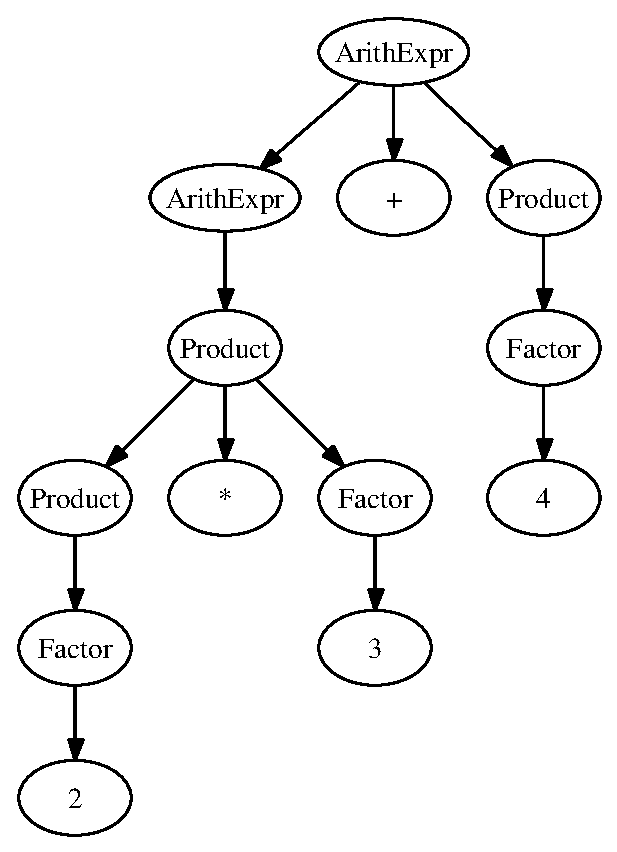
\epsfig{file=Abbildungen/parse-tree.eps, scale=0.7}
  \caption{Ein Parse-Baum f�r den String ``\texttt{2*3+4}''.}
  \label{fig:parse-tree.dot}
\end{figure}

Da B�ume der in Abbildung \ref{fig:parse-tree.dot} gezeigten Art sehr schnell zu gro�
werden, vereinfachen wir diese B�ume mit Hilfe der folgenden Regeln:
\begin{enumerate}
\item Ist $n$ ein innerer Knoten, der mit der Variablen $A$ beschriftet ist
      und gibt es unter den Kindern dieses Knotens genau ein Kind, dass mit einem Terminal $o$
      beschriftet ist,  so entfernen wir dieses Kind und beschriften den Knoten $n$ statt dessen mit dem
      Terminal $o$.
\item Hat ein innerer Knoten nur ein Kind, so ersetzen wir diesen Knoten durch sein Kind.
\end{enumerate}
Den Baum, den wir auf diese Weise erhalten, nennen wir den \emph{abstrakten Syntax-Baum}.
Abbildung \ref{fig:abstract-syntax-tree.dot} zeigt den abstrakten Syntax-Baum den wir
erhalten, wenn wir den in Abbildung \ref{fig:parse-tree.dot} gezeigten Parse-Baum nach
diesen Regeln vereinfachen.  Die in diesem Baum gespeicherte Struktur ist genau das, was
wir brauchen um den arithmetischen Ausdruck ``\texttt{2*3+4}'' auszuwerten, denn der Baum zeigt uns,
in welcher Reihenfolge die Operatoren ausgewertet werden m�ssen.

\begin{figure}[!ht]
  \centering
      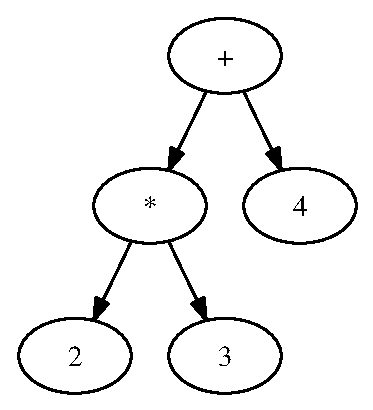
\epsfig{file=Abbildungen/abstract-syntax-tree.eps, scale=0.7}
  \caption{Ein abstrakter Syntax-Baum f�r den String ``\texttt{2*3+4}''.}
  \label{fig:abstract-syntax-tree.dot}
\end{figure}

\subsection{Mehrdeutige Grammatiken}
Die zu Anfang des Abschnitts \ref{kontextfreie} angegebene Grammatik zur Beschreibung arithmetischer
Ausdr�cke erscheint durch ihre Unterscheidung der syntaktischen Kategorien \textsl{arithExpr},
\textsl{product} und \textsl{factor} unn�tig kompliziert.  Wir stellen eine einfachere Grammatik $G$
vor, welche dieselbe Sprache beschreibt:
\\[0.2cm]
\hspace*{1.3cm}
$G = \bigl\langle \{\textsl{expr}\}, \{ \textsc{Number}, \textsc{Variable}, \quoted{+}, \quoted{-}, \quoted{*}, \quoted{/}, \quoted{(}, \quoted{)} \}, R, \textsl{expr} \bigr\rangle$,
\\[0.2cm]
wobei die Regeln $R$ wie folgt gegeben sind:
\begin{eqnarray*}
  \textsl{expr} & \rightarrow & \textsl{expr} \quoted{+} \textsl{expr}  \\
                & \mid        & \textsl{expr} \quoted{-} \textsl{expr}  \\
                & \mid        & \textsl{expr} \quoted{*} \textsl{expr}  \\
                & \mid        & \textsl{expr} \quoted{/} \textsl{expr}  \\
                & \mid        & \quoted{(} \textsl{expr} \quoted{)}     \\
                & \mid        & \textsc{Number}                         \\
                & \mid        & \textsc{Variable}                         
\end{eqnarray*}
Um zu zeigen, dass der String ``\texttt{2*3+4}'' in der von dieser Sprache erzeugten
Grammatik liegt, geben wir die folgende Ableitung an:
\begin{eqnarray*}
\textsl{expr} & \Rightarrow & \textsl{expr} \quoted{+} \textsl{expr}                           \\
              & \Rightarrow & \textsl{expr} \quoted{*} \textsl{expr} \quoted{+} \textsl{expr}  \\
              & \Rightarrow & \texttt{2} \quoted{*} \textsl{expr} \quoted{+} \textsl{expr}     \\
              & \Rightarrow & \texttt{2} \quoted{*} \texttt{3} \quoted{+} \textsl{expr}        \\
              & \Rightarrow & \texttt{2} \quoted{*} \texttt{3} \quoted{+} \texttt{4}           
\end{eqnarray*}
Diese Ableitung entspricht dem abstrakten Syntax-Baum, der in Abbildung
\ref{fig:abstract-syntax-tree.dot}
gezeigt ist.  Es gibt aber noch eine andere Ableitung des Strings ``\texttt{2*3+4}'' mit dieser Grammatik:
\begin{eqnarray*}
\textsl{expr} & \Rightarrow & \textsl{expr} \quoted{*} \textsl{expr}                           \\
              & \Rightarrow & \textsl{expr} \quoted{*} \textsl{expr} \quoted{+} \textsl{expr}  \\
              & \Rightarrow & \texttt{2} \quoted{*} \textsl{expr} \quoted{+} \textsl{expr}     \\
              & \Rightarrow & \texttt{2} \quoted{*} \texttt{3} \quoted{+} \textsl{expr}        \\
              & \Rightarrow & \texttt{2} \quoted{*} \texttt{3} \quoted{+} \texttt{4}           
\end{eqnarray*}
Dieser Ableitung entspricht der abstrakte Syntax-Baum, der in Abbildung
\ref{fig:abstract-syntax-tree-prod.dot} gezeigt ist.
Bei dieser Ableitung wird der String ``\texttt{2*3+4}'' offenbar als Produkt aufgefasst,
was der Konvention widerspricht, dass der Operator ``\texttt{*}'' st�rker bindet als der Operator
``\texttt{+}''.  W�rden wir den String an Hand des letzten Syntax-Baums auswerten, w�rden wir
offenbar ein falsches Ergebnis bekommen! 
\begin{figure}[!ht]
  \centering
      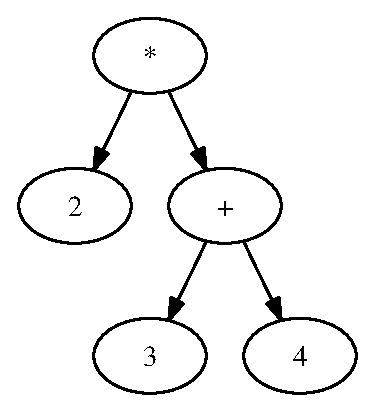
\epsfig{file=Abbildungen/abstract-syntax-tree-prod.eps, scale=0.6}
  \caption{Ein anderer abstrakter Syntax-Baum f�r den String ``\texttt{2*3+4}''.}
  \label{fig:abstract-syntax-tree-prod.dot}
\end{figure}
Die Ursache dieses Problems ist die Tatsache, dass die zuletzt angegebene Grammatik \underline{mehrdeuti}g ist.
Eine solche Grammatik ist zum Parsen ungeeignet.  Leider ist die Frage, ob eine gegebene
Grammatik mehrdeutig ist, im Allgemeinen nicht
\href{http://en.wikipedia.org/wiki/Ambiguous_grammar#Recognizing_ambiguous_grammars}{entscheidbar}:
Es l�sst sich zeigen, dass diese Frage zum
\href{http://en.wikipedia.org/wiki/Post_correspondence_problem}{\emph{Postschen Korrespondenz-Problem}} 
�quivalent ist.  Da das Postsche Korrespondenz-Problem als unl�sbar nachgewiesen wurde, ist auch die
Frage, ob eine Grammatik mehrdeutig ist, unl�sbar.
Ein Beweis dieser Behauptungen findet sich beispielsweise in dem Buch von Hopcroft, Motwani und
Ullman \cite{hopcroft:06}. 


\example
Es sei $\Sigma = \{ \squoted{A}, \squoted{B} \}$.  Die Sprache $L$ enthalte alle die W�rter
aus $\Sigma^*$, bei denen die Buchstaben \squoted{A} and \squoted{B} mit der gleichen
H�ufigkeit auftreten, es gilt also
\\[0.2cm]
\hspace*{1.3cm}
$L = \bigl\{ w \in \Sigma^* \mid \textsl{count}(w, \squoted{A}) = \textsl{count}(w, \squoted{B}) \bigr\}$.
\\[0.2cm]
Dann wird die Sprache $L$ durch die kontextfreie Grammatik $G_1 = \langle \{s\}, \Sigma, R_1, s \rangle$ beschrieben,
deren Regeln wie folgt gegeben sind:
\\[0.2cm]
\hspace*{1.3cm}
$\textsl{s} \;\rightarrow\; \quoted{A} s \quoted{B} s \;\mid\; \quoted{B} s \quoted{A} s \;\mid\; \varepsilon$
\\[0.2cm]
Der Grund ist, dass ein String $w \in L$ entweder mit einem \squoted{A} oder mit einem \squoted{B}
beginnt.  Im ersten Fall muss es zu diesem \squoted{A} ein korrespondierendes \squoted{B} geben, denn
die Anzahl der Auftreten von \squoted{A} und \squoted{B} sind gleich.  Fassen wir den Buchstaben
\squoted{A} wie eine �ffnende Klammer auf und interpretieren den Buchstaben \squoted{B} als die zu
\squoted{A} korrespondierende schlie�ende Klammer, so ist klar, dass der String, der zwischen diesen
beiden Auftreten von \squoted{A} und \squoted{B} liegt, ebenfalls gleich viele Auftreten von
\squoted{A} wie von \squoted{B} hat.  Genauso muss dies dann f�r den Rest des Strings gelten, der nach
dem \squoted{B} folgt.  Diese �berlegung erkl�rt die Regel
\\[0.2cm]
\hspace*{1.3cm}
$\textsl{s} \;\rightarrow\; \quoted{A} s \quoted{B} s$
\\[0.2cm]
Die Regel
\\[0.2cm]
\hspace*{1.3cm}
$\textsl{s} \;\rightarrow\; \quoted{B} s \quoted{A} s$
\\[0.2cm]
l�sst sich in analoger Weise erkl�ren,  wenn wir den Buchstaben \squoted{B} als �ffnende Klammer und
\squoted{A} als schlie�ende Klammer interpretieren. 

Diese Grammatik ist allerdings mehrdeutig: Betrachten wir beispielsweise den String 
``\texttt{abab}'', so stellen wir fest, dass sich dieser prinzipiell auf zwei Arten ableiten l�sst:
\begin{eqnarray*}
  s & \Rightarrow &\quoted{A} s \quoted{B} s                       \\
    & \Rightarrow &\quoted{A} \quoted{B} s                         \\
    & \Rightarrow &\quoted{A} \quoted{B}\quoted{A} s \quoted{B} s \\
    & \Rightarrow &\quoted{A} \quoted{B}\quoted{A} \quoted{B} s   \\
    & \Rightarrow &\quoted{A} \quoted{B}\quoted{A} \quoted{B} 
\end{eqnarray*}
Eine andere Ableitung des selben Strings ergibt sich, wenn wir im zweiten Ableitungs-Schritt nicht das erste
$s$ durch $\varepsilon$ ersetzen sondern statt dessen das zweite $s$ durch $\varepsilon$ ersetzen:
\begin{eqnarray*}
  s & \Rightarrow &\quoted{A} s \quoted{B} s                       \\
    & \Rightarrow &\quoted{A} s \quoted{B}                         \\
    & \Rightarrow &\quoted{A} \quoted{B} s\quoted{A} s \quoted{B} \\
    & \Rightarrow &\quoted{A} \quoted{B}\quoted{A} s \quoted{B}   \\
    & \Rightarrow &\quoted{A} \quoted{B}\quoted{A} \quoted{B}     \\
\end{eqnarray*}
Abbildung \ref{fig:ambiguous-a.dot} zeigt die Parse-B�ume, die sich aus den beiden Ableitungen ergeben.
Wir k�nnen erkennen, dass die Struktur dieser B�ume unterschiedlich ist:  Im ersten Fall geh�rt das erste
``\texttt{A}'' zu dem ersten ``\texttt{B}'', im zweiten Fall geh�rt das erste ``\texttt{A}'' zu dem letzten
``\texttt{B}''.

\begin{figure}[!ht]
      \epsfig{file=Abbildungen/ambiguous-a.eps, scale=0.6}
\quad
      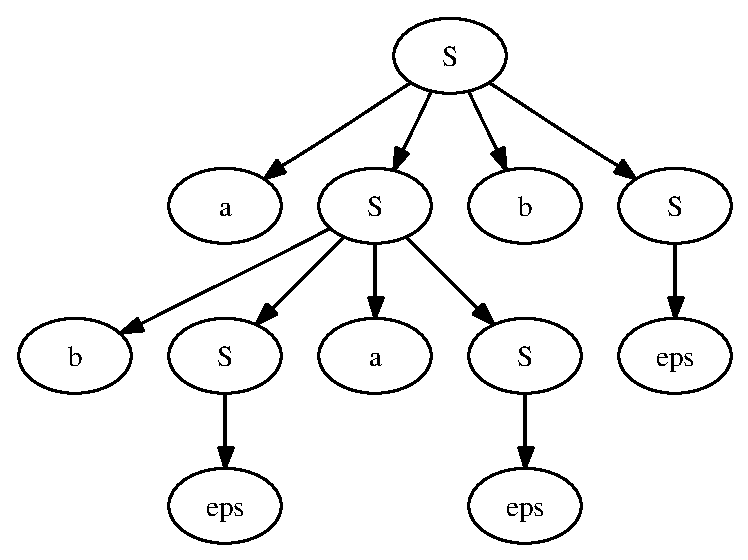
\epsfig{file=Abbildungen/ambiguous-b.eps, scale=0.6}
  \caption{Zwei strukturell verschiedene Parse-B�ume f�r den String ``\texttt{ABAB}''.}
  \label{fig:ambiguous-a.dot}
\end{figure}

Wir definieren nun eine  kontextfreie Grammatik $G_2 = \langle \{s, u, v, x, y\}, \Sigma, R_2, s \rangle$,
deren Regeln wie folgt gegeben sind:
\hspace*{1.3cm}
\begin{eqnarray*}
\textsl{s} & \rightarrow & u s \;\mid\; v s  \;\mid\; \varepsilon \\[0.2cm]
\textsl{u} & \rightarrow &\quoted{A} x \quoted{B}                \\[0.2cm]
\textsl{v} & \rightarrow & \quoted{B} y\quoted{A}                \\[0.2cm]
\textsl{x} & \rightarrow & \textsl{u} \textsl{x} \;\mid\; \varepsilon \\[0.2cm]
\textsl{y} & \rightarrow & \textsl{v} \textsl{y} \;\mid\; \varepsilon          
\end{eqnarray*}
Um die Sprachen, die von den einzelnen Variablen erzeugt werden, klarer beschreiben zu
k�nnen, definieren wir f�r zwei Strings $\sigma$ und $\omega$ die Relation $\sigma \preceq \omega$ (lese: $\sigma$ ist ein
Pr�fix von $\omega$) wie folgt:
\\[0.2cm]
\hspace*{1.3cm}
$\sigma \preceq \omega \quad \stackrel{\rm{def}}{\Longleftrightarrow} \exists \tau \in \Sigma^*: \sigma \tau = \omega$
\\[0.2cm]
Sodann bemerken wir, dass von den syntaktischen Variablen $x$ und $y$ die folgenden
Sprachen erzeugt werden:
\\[0.2cm]
\hspace*{1.3cm} 
$L(x) = \bigl\{ \omega \in \Sigma^* \mid \omega \in L \;\wedge\; \forall \sigma \preceq \omega : 
                  \textsl{count}(\sigma,\squoted{B}) \leq \textsl{count}(\sigma,\squoted{A}) \bigr\}$
\quad und \\[0.2cm]
\hspace*{1.3cm}
$L(y) = \bigl\{ \omega \in \Sigma^* \mid \omega \in L \;\wedge\; \forall \sigma \preceq \omega : 
                  \textsl{count}(\sigma, \squoted{A}) \leq \textsl{count}(\sigma, \squoted{B}) \bigr\}$.
\\[0.2cm]
Ein String der Sprache $L(x)$ kann also kein ``\texttt{B}'' enthalten, dass zu einem
``\texttt{A}'' geh�rt, das vor diesem String steht und analog kann 
ein String der Sprache $L(y)$  kein ``\texttt{A}'' enthalten, dass zu einem
``\texttt{B}'' geh�rt, das vor diesem String steht.

Ein String der Sprache $L$ f�ngt nun entweder mit ``\texttt{A}'' oder mit ``\texttt{B}''
an.  Im ersten Fall interpretieren wir das ``\texttt{A}'' als �ffnende Klammer und 
das ``\texttt{B}'' als schlie�ende Klammer und suchen nun das ``\texttt{B}'', das dem
``\texttt{A}'' am Anfang des Strings zugeordnet ist.  Der String, der mit dem
``\texttt{A}'' anf�ngt und dem ``\texttt{B}'' endet, liegt in der Sprache $L(u)$.
Auf dieses ``\texttt{B}'' kann dann noch ein weiterer Teilstring folgen, der
gleich viele ``\texttt{A}''s und ``\texttt{B}''s enth�lt.  Ein solcher Teilstring liegt
offensichtlich ebenfalls in der Sprache $L$ und kann daher von $s$ mittels der Regel
\\[0.2cm]
\hspace*{1.3cm}
$\textsl{s} \rightarrow \textsl{u}\textsl{s}$
\\[0.2cm]
erzeugt werden.
Im zweiten Fall f�ngt der String mit einem ``\texttt{B}'' an.  Dieser Fall ist
analog zum ersten Fall.    \qed
\vspace*{0.3cm}

In dem obigen Beispiel hatten wir Gl�ck und konnten eine Grammatik finden, mit der sich
die Sprache eindeutig parsen l�sst.  Es  gibt allerdings auch kontextfreie Sprachen, die 
\href{http://en.wikipedia.org/wiki/Ambiguous_grammar#Inherently_ambiguous_languages}{inh�rent mehrdeutig}
sind: Es l�sst sich beispielsweise zeigen, dass f�r das Alphabet 
$\Sigma =  \{ \squoted{A}, \squoted{B}, \squoted{C}, \squoted{D} \}$
die Sprache
\\[0.2cm]
\hspace*{1.3cm}
$L =  \bigl\{ \mathtt{A}^m \mathtt{B}^m \mathtt{C}^n \mathtt{D}^n \mid m, n \in \mathbb{N} \bigr\}
 \cup \bigl\{ \mathtt{A}^m \mathtt{B}^n \mathtt{C}^n \mathtt{D}^m \mid m, n \in \mathbb{N} \bigr\}
$
\\[0.2cm]
kontextfrei ist, aber jede Grammatik $G$ mit der Eigenschaft $L = L(G)$ ist
notwendigerweise mehrdeutig.  Das Problem ist, dass f�r gewisse gro�e Zahlen $n\in \mathbb{N}$ ein
String der Form 
\\[0.2cm]
\hspace*{1.3cm}
$\mathtt{A}^n \mathtt{B}^n \mathtt{C}^n \mathtt{D}^n$
\\[0.2cm]
immer zwei strukturell verschiedene Parse-B�ume besitzt.  Ein Beweis dieser Behaupung
findet sich in dem Buch von  Hopcroft und Ullman auf Seite 100 \cite{hopcroft:79}.   

\section{Top-Down-Parser}
In diesem Abschnitt stellen wir ein Verfahren vor, mit dem sich viele
Grammatiken leicht parsen lassen.  Die Grundidee ist einfach:  Um einen String $w$ mit
Hilfe einer Grammatik-Regel der Form
\\[0.2cm]
\hspace*{1.3cm}
$\textsl{a} \rightarrow \textsl{X}_1 \textsl{X}_2 \cdots \textsl{X}_n$
\\[0.2cm]
zu parsen, versuchen wir, zun�chst ein $X_1$ zu parsen.  Dabei zerlegen wir den String $w$ in die
Form
$w = w_1 r_1$ so, dass $w_1 \in L(X_1)$ liegt.  Dann versuchen wir, in dem Rest-String
$r_1$ ein $X_2$ zu parsen und zerlegen dabei $r_1$ so, dass $r_1 = w_2 r_2$ mit 
$w_2 \in L(X_2)$ gilt.  Setzen wir diesen Prozess fort, so haben wir zum Schluss den String $w$ in
\\[0.2cm]
\hspace*{1.3cm}
$w = w_1 w_2 \cdots w_n$ \quad mit $w_i \in L(X_i)$ f�r alle $i=1,\cdots,n$
\\[0.2cm]
aufgespaltet.  Leider funktioniert dieses Verfahren dann nicht, wenn die Grammatik
\emph{links-rekursiv} ist, dass hei�t, dass eine Regel die Form
\\[0.2cm]
\hspace*{1.3cm}
$\textsl{a} \rightarrow \textsl{a} \beta$
\\[0.2cm]
hat, denn dann w�rden wir um ein $\textsl{a}$ zu parsen sofort wieder rekursiv versuchen, 
ein $a$ zu parsen und w�ren damit in einer Endlos-Schleife.  Es gibt mehrere M�glichkeiten, um mit
diesem Problem umzugehen:
\begin{enumerate}
\item Wir k�nnen die Grammatik so umschreiben, dass sie danach nicht mehr links-rekursiv
      ist.
\item Wir k�nnen versuchen, den String \emph{r�ckw�rts} zu parsen, d.h.~bei einer
      Regel der Form
      \\[0.2cm]
      \hspace*{1.3cm}
      $\textsl{a} \rightarrow \textsl{X}_1 \textsl{X}_2 \cdots \textsl{X}_n$
      \\[0.2cm]
      versuchen wir als erstes, ein $X_n$ am Ende eines zu parsenden Strings $w$ zu
      entdecken und arbeiten dann den String $w$ von hinten  nach vorne ab.  
\item Die einfachste L�sung erhalten wir, wenn wir uns klar machen, dass kontextfreie
      Grammatiken nicht unbedingt die bequemste Art darstellen, eine Sprache 
      zu beschreiben.  Wir werden daher den Begriff der \emph{erweiterten Backus-Naur-Form}-Grammatik
      (abgek�rzt \textsc{Ebnf}-Grammatik) einf�hren.  Hierbei handelt es sich um eine Verallgemeinerung des
      Begriffs der kontextfreien Grammatik.  Theoretisch ist die Ausdrucksst�rke der
      \textsc{Ebnf}-Grammatiken dieselbe wie die Ausdrucksst�rke der kontextfreien Grammatiken.
      In der Praxis zeigt sich aber, dass die Konstruktion von Top-Down-Parsern f�r
      \textsc{Ebnf}-Grammatiken einfacher ist, weil dort die Links-Rekursion durch eine Iteration ersetzt
      werden kann.
\end{enumerate}
Im Rahmen dieses Kapitels werden wir alle oben genannten Verfahren an Hand der Grammatik f�r
arithmetische Ausdr�cke ausf�hrlich diskutieren.  

\subsection{Umschreiben der Grammatik$^*$ \label{links-rekursion}}
In der folgenden Grammatik ist $a$ eine syntaktische Variable und die griechischen Buchstaben $\beta$ und
$\gamma$ stehen f�r irgendwelche Strings, die aus syntaktischen Variablen und Tokens bestehen.
Wird die syntaktische Variable $a$ durch die beiden Regeln
\\[0.2cm]
\hspace*{1.3cm}
$
\begin{array}[t]{lcl}
a & \rightarrow & a \beta \\
  & \mid        & \gamma
\end{array}
$
\\[0.2cm]
definiert, so hat eine Ableitung von $a$, bei der zun�chst immer die syntaktische Variable $a$ ersetzt
wird, die Form 
\\[0.2cm]
\hspace*{1.3cm}
$a \Rightarrow a \beta \Rightarrow a \beta \beta \Rightarrow a \beta \beta \beta
 \Rightarrow \cdots \Rightarrow a \beta^n \Rightarrow \gamma \beta^n$.
\\[0.2cm]
Damit sehen wir, dass die durch die syntaktische Variable $a$ beschriebene Sprache $L(a)$ aus alle den
Strings besteht, die sich aus dem Ausdruck $\gamma \beta^n$ ableiten lassen:
\\[0.2cm]
\hspace*{1.3cm}
$L(a) = \bigl\{ w \in \Sigma^* \mid \exists n \in \mathbb{N}_0: \gamma \beta^n \Rightarrow^* w \bigr\}$.
\\[0.2cm]
Diese Sprache kann offenbar auch durch die folgenden Regeln f�r $a$ beschrieben werden:
\\[0.2cm]
\hspace*{1.3cm}
$
\begin{array}[t]{lcl}
a & \rightarrow & \gamma b \\[0.2cm]
b & \rightarrow & \beta b  \\
  & \mid        & \varepsilon 
\end{array}
$
\\[0.2cm]
Hier haben wir die Hilfs-Variable $b$ eingef�hrt.  Die Ableitungen, die von dem Nicht-Terminal $b$
ausgehen, haben die Form
\\[0.2cm]
\hspace*{1.3cm} $b \Rightarrow \beta b \Rightarrow \beta \beta b \Rightarrow \cdots \Rightarrow
\beta^n b \Rightarrow \beta^n$.
\\[0.2cm]
Folglich beschreibt das Nicht-Terminal $b$ die Sprache
\\[0.2cm]
\hspace*{1.3cm} $L(b) = \bigl\{ w \in \Sigma \mid \exists n \in \mathbb{N}_0: \beta^n \Rightarrow w
\bigr\}$.
\\[0.2cm]
Damit ist klar, dass auch mit der oben angegeben Grammatik
\\[0.2cm]
\hspace*{1.3cm} $L(a) = \bigl\{ w \in \Sigma^* \mid \exists n \in \mathbb{N}_0: \gamma \beta^n
\Rightarrow^* w \bigr\}$
\\[0.2cm]
gilt.  Um die Links-Rekursion aus der in Abbildung \ref{fig:Expr} auf Seite \pageref{fig:Expr}
gezeigten Grammatik zu entfernen, m�ssen wir das obige Beispiel verallgemeinern.  Wir betrachten
jetzt den allgemeinen Fall und nehmen an, dass ein Nicht-Terminal $a$ durch Regeln der Form
\\[0.2cm]
\hspace*{1.3cm} $
\begin{array}[t]{lcl}
a & \rightarrow & a \beta_1 \\
  & \mid        & a \beta_2 \\
  & \vdots      & \vdots    \\
  & \mid        & a \beta_k \\[0.2cm]
  & \mid        & \gamma_1  \\
  & \vdots      & \vdots    \\
  & \mid        & \gamma_l
\end{array}
$
\\[0.2cm]
beschrieben wird.  Wir k�nnen diesen Fall durch Einf�hrung zweier Hilfs-Variablen $b$ und $c$ auf
den ersten Fall zur�ckf�hren:
\\[0.2cm]
\hspace*{1.3cm}
$
\begin{array}[t]{lcl}
a & \rightarrow & a b \mid c                         \\[0.2cm]
b & \rightarrow & \beta_1 \mid \cdots \mid \beta_k   \\[0.2cm]
c & \rightarrow & \gamma_1 \mid \cdots \mid \gamma_l
\end{array}
$
\\[0.2cm]
Dann k�nnen wir die Grammatik umschreiben, indem wir eine neue Hilfs-Variablen, nennen wir sie $l$
f�r Liste, einf�hren und erhalten
\\[0.2cm]
\hspace*{1.3cm}
$
\begin{array}[t]{lcl}
a & \rightarrow & c\;l                   \\[0.2cm]
l & \rightarrow & b\;l \mid \varepsilon.  
\end{array}
$
\\[0.2cm]
Die Hilfs-Variablen $b$ und $c$ k�nnen nun wieder eliminiert werden und dann bekommen wir die folgende
Grammatik: 
\\[0.2cm]
\hspace*{1.3cm}
$
\begin{array}[t]{lcl}
a & \rightarrow & \gamma_1\;l \;\mid\; \gamma_2\;l \;\mid\; \cdots \;\mid\; \gamma_l\;l  \\[0.2cm]
l & \rightarrow & \beta_1 \;l \;\mid\; \beta_2 \;l \;\mid\; \cdots \;\mid\; \beta_k \;l \;\mid\; \varepsilon
\end{array}
$
\begin{figure}[htbp]
  \begin{center}    
  \framebox{
  \framebox{
  \begin{minipage}[t]{8cm}
  \begin{eqnarray*}
  \textsl{expr}    & \rightarrow & \;\textsl{expr} \quoted{+} \textsl{product}  \\
                   & \mid        & \;\textsl{expr} \quoted{-} \textsl{product}  \\
                   & \mid        & \;\textsl{product}                           \\[0.2cm]
  \textsl{product} & \rightarrow & \;\textsl{product} \quoted{*} \textsl{factor}\\
                   & \mid        & \;\textsl{product} \quoted{/} \textsl{factor}\\
                   & \mid        & \;\textsl{factor}                            \\[0.2cm]
  \textsl{factor}  & \rightarrow &   \quoted{(} \textsl{expr} \quoted{)}        \\
                   & \mid        & \;\textsc{Number} 
  \end{eqnarray*}
  \vspace*{-0.5cm}
  \end{minipage}}}
  \end{center}
  \caption{Links-rekursive Grammatik f�r arithmetische Ausdr�cke.}
  \label{fig:Expr}
\end{figure}
\vspace*{0.3cm}

\noindent
Wenden wir dieses Verfahren auf die in Abbildung \ref{fig:Expr} gezeigte Grammatik f�r arithmetische
Ausdr�cke an, so erhalten wir die in Abbildung \ref{fig:Expr2} gezeigte Grammatik.

\begin{figure}[htbp]
  \begin{center}    
  \framebox{
  \framebox{
  \begin{minipage}[t]{9cm}
  \begin{eqnarray*}
  \textsl{expr}        & \rightarrow & \;\textsl{product}\;\;\textsl{exprRest}            \\[0.2cm]
  \textsl{exprRest}    & \rightarrow & \quoted{+} \textsl{product}\;\;\textsl{exprRest}   \\
                       & \mid        & \quoted{-} \textsl{product}\;\;\textsl{exprRest}   \\
                       & \mid        & \;\varepsilon                                      \\[0.2cm]
  \textsl{product}     & \rightarrow & \;\textsl{factor}\;\;\textsl{productRest}          \\[0.2cm]
  \textsl{productRest} & \rightarrow & \quoted{*} \textsl{factor}\;\;\textsl{productRest} \\
                       & \mid        & \quoted{/} \textsl{factor}\;\;\textsl{productRest} \\
                       & \mid        & \;\varepsilon                                      \\[0.2cm]
  \textsl{factor}      & \rightarrow & \quoted{(} \textsl{expr} \quoted{)}                \\
                       & \mid        & \;\textsc{Number} 
  \end{eqnarray*}
  \vspace*{-0.5cm}
  \end{minipage}}}
  \end{center}
  \caption{Grammatik f�r arithmetische Ausdr�cke ohne Links-Rekursion.}
  \label{fig:Expr2}
\end{figure}

\noindent
Die Variablen \textsl{exprRest} und \textsl{productRest} k�nnen wie folgt interpretiert werden:
\begin{enumerate}
\item \textsl{exprRest} beschreibt eine Liste der Form
      \\[0.2cm]
      \hspace*{1.3cm}
      $\textsl{op} \;\textsl{product} \;\cdots \;\textsl{op}\; \textsl{product}$,
      \\[0.2cm]
      wobei $\textsl{op} \in \{ \quoted{+}, \quoted{-} \}$ gilt.
\item \textsl{productRest} beschreibt eine Liste der Form
      \\[0.2cm]
      \hspace*{1.3cm}
      $\textsl{op} \;\textsl{factor} \;\cdots \;\textsl{op} \;\textsl{factor}$,
      \\[0.2cm]
      wobei $\textsl{op} \in \{ \quoted{*}, \quoted{/} \}$ gilt. 
\end{enumerate}


\exercise
\begin{enumerate}
\item[(a)] Die folgende Grammatik beschreibt regul�re Ausdr�cke:
      \begin{center}    
          \framebox{
            \begin{minipage}[t]{9cm}
              \begin{eqnarray*}
                \textsl{regExp} & \rightarrow & \;\textsl{regExp} \quoted{+} \textsl{regExp}    \\
                                & \mid        & \;\textsl{regExp} \;\;\textsl{regExp}           \\
                                & \mid        & \;\textsl{regExp}\quoted{*}                     \\
                                & \mid        & \quoted{(} \textsl{regExp} \quoted{)}           \\
                                & \mid        & \;\textsc{Letter}                               
              \end{eqnarray*}
              \vspace*{-0.5cm}
            \end{minipage}}
      \end{center}
      Diese Grammatik verwendet nur die  syntaktische Variable $\{ \textsl{regExp} \}$ und die folgenden 
      Terminale
      \\[0.2cm]
      \hspace*{1.3cm}
      \squoted{+}, \squoted{*}, \squoted{(}, \squoted{)}, \textsc{Letter}.
      \\[0.2cm]
      Da die Grammatik mehrdeutig ist, ist diese Grammatik zum Parsen ungeeignet.
      Transformieren Sie diese Grammatik in eine eindeutige Grammatik, bei welcher der
      Postfix-Operator ``\texttt{*}'' st�rker bindet als die Konkatenation zweier regul�rer
      Ausdr�cke, w�hrend der Operator ``\texttt{+}'' schw�cher bindet als die Konkatenation. 
      Orientieren Sie sich dabei an der Grammatik f�r arithmetische Ausdr�cke und f�hren
      Sie geeignete neue syntaktische Variablen ein.
\item[(b)] Entfernen Sie die Links-Rekursion aus der in Teil (a) dieser Aufgabe erstellten
      Grammatik. \eox
\end{enumerate}

\begin{figure}[htbp]
  \begin{center}    
  \framebox{
  \framebox{
  \begin{minipage}[t]{9cm}
  \begin{eqnarray*}
  \textsl{s}  & \rightarrow & \textsl{a} \quoted{X}  \\
              & \mid        & \squoted{Y}            \\[0.2cm]
  \textsl{a}  & \rightarrow & \textsl{b} \quoted{Y}  \\
              & \mid        & \quoted{x}             \\[0.2cm]
  \textsl{b}  & \rightarrow & \textsl{s} \quoted{Z}  
  \end{eqnarray*}
  \vspace*{-0.5cm}
  \end{minipage}}}
  \end{center}
  \caption{Wechselseitige Links-Rekursion.}
  \label{fig:mutual-left-recursion}
\end{figure}

Bei den bisher diskutierten Beispielen war die Links-Rekursion der Grammatik unmittelbar anzusehen.
Es gibt allerdings F�lle, in denen die Links-Rekursion ihren Ursprung in 
\emph{wechselseitiger Rekursion} hat.
Abbildung \ref{fig:mutual-left-recursion} auf Seite \pageref{fig:mutual-left-recursion} zeigt ein
solches Beispiel: Bei der dort angegebenen Grammatik erstreckt sich die Links-Rekursion �ber drei Stufen:
Ein $s$ kann mit einem $a$ beginnen, das mit einem $b$ beginnen kann, welches dann wieder mit einem
$s$ beginnt.  Eine Links-Rekursion der Form
\\[0.2cm]
\hspace*{1.3cm}
$a \rightarrow a \beta$
\\[0.2cm]
bezeichnen wir als \emph{unmittelbare Links-Rekursion},  jede kompliziertere Form der
Links-Rekursion wird als \emph{allgemeine Links-Rekursion} bezeichnet.
Um allgemeine Links-Rekursion zu eliminieren, gehen wir wie folgt vor:
\begin{enumerate}
\item Zun�chst numerieren wir die syntaktischen Variablen der Grammatik in willk�rlicher Weise durch.
      Im Folgenden seien die Variablen mit $a_1$, $\cdots$, $a_n$ bezeichnet.  Durch diese
      Numerierung wird implizit eine Ordnung $\succ$ auf den syntaktischen Variablen
      definiert, wir setzen
      \\[0.2cm]
      \hspace*{1.3cm}
      $a_1 \succ a_2 \succ \cdots \succ a_i \succ a_{i+1} \succ \cdots \succ a_n$.
\item Das Ziel ist nun, die Grammatik so umzuschreiben, dass f�r jede
      Grammatik-Regel der Form
      \\[0.2cm]
      \hspace*{1.3cm}
      $a \rightarrow b \gamma$ \quad die Ungleichung \quad $a \succ b$
      \\[0.2cm]
      gilt.  Dieses Ziel wird durch den folgenden Algorithmus erreicht:
      \\[0.2cm]
      \hspace*{1.3cm}
      \texttt{for (i = 1; i <= n; ++i) \{}  \\[0.1cm]
      \hspace*{1.8cm}
      \texttt{for (j = 1; j < i; ++j) \{} \\[0.1cm]
      \hspace*{2.3cm}
      \texttt{forall $(a_i \rightarrow a_j\gamma) \in R$ \{} \\[0.1cm]
      \hspace*{2.8cm}
      \texttt{let $a_j \rightarrow \delta_1 \;|\; \cdots \;|\; \delta_k$ be all $a_j$-productions } \\[0.1cm]
      \hspace*{2.8cm}
      \texttt{replace $a_i \rightarrow a_j\gamma$ by $a_i \rightarrow \delta_1 \gamma \;|\;\cdots\;|\;\delta_k \gamma$} \\[0.1cm]
      \hspace*{2.3cm} 
      \texttt{\}}  \\[0.1cm]
      \hspace*{1.8cm} 
      \texttt{\}}  \\[0.1cm]
      \hspace*{1.8cm} 
      \texttt{eliminate immediate left recursion for variable $a_i$}  \\
      \hspace*{1.3cm} 
      \texttt{\}}  
\end{enumerate}
Um den Algorithmus zu verstehen, f�hren wir zun�chst einen neuen Begriff ein:  Falls die Grammatik
eine Regel der Form
\\[0.2cm]
\hspace*{1.3cm}
$a \rightarrow b \gamma$
\\[0.2cm]
enth�lt, wobei $b$ eine syntaktische Variable ist, dann sagen wir, dass $a$ unmittelbar von $b$
abh�ngt.  Die Idee bei dem oben angegebenen Algorithmus ist nun, dass nach dem $i$-ten
Durchlaufen der �u�eren \texttt{for}-Schleife die Variablen $a_1$, $\cdots$, $a_i$ nur noch unmittelbar
von solchen Variablen abh�ngen, die in der Aufz�hlung $a_1$, $\cdots$, $a_n$ auf diese  Variablen
folgen.  Formal gilt nach dem $i$-ten Durchlauf der �u�eren \texttt{for}-Schleife f�r alle Indizes 
$k \in \{ 1, \cdots, i \}$:  Falls die Grammatik eine Regel der Form
\\[0.2cm]
\hspace*{1.3cm}
$a_k \rightarrow a_l \beta$ 
\\[0.2cm]
enth�lt, dann muss $l > k$ gelten.  Es ist leicht zu sehen, dass diese Invariante tats�chlich gilt:
Vor dem $i$-ten Durchlauf gilt die Invariante f�r die Indizes der Menge $\{1, \cdots, i-1\}$.  Die
Variable $a_i$ selber kann dann noch unmittelbar von den Variablen $a_1$, $\cdots$, $a_n$ abh�ngen.
In der inneren \texttt{for}-Schleife erreichen wir, dass nacheinander die unmittelbaren
Abh�ngigkeiten von $a_1$, $\cdots$, $a_{i-1}$ aufgel�st werden.  Anschlie�end kann $a_i$ h�chstens
noch unmittelbar von $a_i$ abh�ngen.  Um diese Abh�ngigkeit gegebenenfalls aufzul�sen, f�hren wir
die bereits fr�her diskutierte Transformation zur Elimination unmittelbarer Links-Rekursion durch.
Anschlie�end h�ngt $a_i$ h�chstens noch 
unmittelbar von $a_{i+1}$, $\cdots$, $a_n$ ab.  L�uft die Schleife bis zum Ende durch, ist damit
die Links-Rekursion vollst�ndig eliminiert, denn dann kann jede Variable nur von solchen
Variablen abh�ngen, die in der Aufz�hlung $a_1$ $\cdots$, $a_n$ hinter ihr stehen.  Folglich ist 
kein Zyklus der Form 
\\[0.2cm]
\hspace*{1.3cm}
$a_i \Rightarrow a_j\beta \Rightarrow \cdots \Rightarrow a_i\gamma$
\\[0.2cm]
mehr m�glich.

\example
Wir demonstrieren das Verfahren an der in Abbildung \ref{fig:mutual-left-recursion} gezeigten
Grammatik.  Dazu ordnen wir zun�chst die Variablen in der Form
\\[0.2cm]
\hspace*{1.3cm}
$s, a, b$
\\[0.2cm]
an, mit der Notation des oben angegebenen Algorithmus gilt also $a_1 := s$, $a_2 := a$ und 
$a_3 := b$.
\begin{enumerate}
\item $i = 1$:  Da $\{1, \cdots, i-1 \} = \{\}$ gilt,  wird in diesem Fall die innere
      \texttt{for}-Schleife nicht ausgef�hrt.  Wir m�ssen lediglich
      die unmittelbare Links-Rekursion in der Variablen $s$ entfernen.  Da die Grammatik aber f�r
      $s$ keine unmittelbare Links-Rekursion enth�lt, ist in diesem Fall nichts zu tun.
\item $i = 2$:  In diesem Schritt m�ssen wir in der inneren \texttt{for}-Schleife sicherstellen,
      dass $a$ nicht unmittelbar von $s$ abh�ngt.  da $a$ in der gegebenen Grammatik nicht
      unmittelbar von $s$ abh�ngt, ist bei der inneren \texttt{for}-Schleife wieder nichts zu tun.

      Weiter m�ssen wir die unmittelbare Rekursion aus allen Regeln f�r $a$ eliminieren.  Da 
      es f�r die Variable $a$ keine unmittelbare Rekursion gibt, ist an dieser Stelle ebenfalls nichts
      zu tun.
\item $i = 3$:  In diesem Fall kommen f�r die innere \texttt{for}-Schleife zwei Werte von $j$
      in Frage, die wir nacheinander behandeln m�ssen:
      \begin{enumerate}
      \item $j = 1$:  Hier m�ssen wir sicherstellen, dass $b$ nicht unmittelbar von $s$ abh�ngt.
            Bei der Regel
            \\[0.2cm]
            \hspace*{1.3cm}
            $b \rightarrow s \quoted{Z}$
            \\[0.2cm]
            ist dies aber der Fall.  Wir ersetzen daher das $s$ auf der rechten Seite dieser Regel
            durch die beiden rechten Seiten der Regeln f�r $s$ und erhalten f�r $b$ nun die Regeln
            \\[0.2cm]
            \hspace*{1.3cm}
            $b \rightarrow a \quoted{X} \squoted{Z}$ \quad und \quad
            $b \rightarrow \quoted{Y} \squoted{Z}$.
      \item $j = 2$:  Nun m�ssen wir sicherstellen, dass $b$ nicht unmittelbar von $a$ abh�ngt.
            Bei der Regel
            \\[0.2cm]
            \hspace*{1.3cm}
            $b \rightarrow a \quoted{X} \squoted{Z}$ 
            \\[0.2cm]
            ist dies aber der Fall.  Wir ersetzen daher das $a$ auf der rechten Seite dieser Regel
            durch die beiden rechten Seiten der Regeln f�r $a$ und erhalten f�r $b$ nun insgesamt
            die folgenden Regeln:
            \\[0.2cm]
            \hspace*{1.3cm}
            $b \rightarrow b \quoted{Y} \squoted{X}\; \squoted{Z}$, \quad 
            $b \rightarrow \quoted{X} \squoted{X}\; \squoted{Z}$ \quad und \quad
            $b \rightarrow \quoted{Y} \squoted{Z}$.
      \end{enumerate}
      Diese Regeln enthalten nun nur noch ummittelbare Links-Rekursion, die wir mit dem fr�her
      beschriebenen Verfahren eliminieren.  Wir erhalten dann f�r $b$ die Regeln
      \\[0.2cm]
      \hspace*{1.3cm}
      $b \rightarrow \quoted{X} \squoted{X} \; \squoted{Z}\; l$ \quad und \quad
      $b \rightarrow \squoted{Y} \quoted{Z} l$,
      \\[0.2cm]
      wobei die neu eingef�hrte Variable $l$ durch die Regeln
      \\[0.2cm]
      \hspace*{1.3cm}
      $l \rightarrow \quoted{Y} \squoted{X}\; \squoted{Z}\; l$ \quad und \quad 
      $l \rightarrow \varepsilon$
      \\[0.2cm]
      definiert ist.
\end{enumerate}
Abbildung \ref{fig:mutual-left-recursion-2} zeigt die resultierende Grammatik.


\begin{figure}[htbp]
  \begin{center}    
  \framebox{
  \framebox{
  \begin{minipage}[t]{9cm}
  \begin{eqnarray*}
  \textsl{s}  & \rightarrow & \textsl{a} \quoted{X}  \\
              & \mid        & \squoted{Y}            \\[0.2cm]
  \textsl{a}  & \rightarrow & \textsl{b} \quoted{Y}  \\
              & \mid        & \squoted{X}             \\[0.2cm]
  \textsl{b}  & \rightarrow & \squoted{X} \quoted{X} \squoted{Z}\; \textsl{l} \\
              & \mid        & \squoted{Y} \quoted{Z} \textsl{l}               \\[0.2cm]
  \textsl{l}  & \rightarrow & \squoted{Y} \quoted{X} \squoted{Z}\; \textsl{l} \\
              & \mid        & \varepsilon      
  \end{eqnarray*}
  \vspace*{-0.5cm}
  \end{minipage}}}
  \end{center}
  \caption{Grammatik ohne Links-Rekursion.}
  \label{fig:mutual-left-recursion-2}
\end{figure}

Das letzte Beispiel zeigt, dass sich eine Grammatik durch die Elimination indirekter Links-Rekursion
stark aufbl�hen kann.  Zwar sind viele Grammatiken links-rekursiv, aber in der Regel
handelt es sich dabei um direkte Links-Rekursion.  Wechselseitige Links-Rekursion ist in den
Grammatiken, die Ihnen in der Praxis begegnen werden, ein eher seltenes Ph�nomen.


\subsection{Implementing a Top Down Parser in \textsc{SetlX}}


\begin{figure}[!ht]
\centering
\begin{Verbatim}[ frame         = lines, 
                  framesep      = 0.3cm, 
                  firstnumber   = 1,
                  labelposition = bottomline,
                  numbers       = left,
                  numbersep     = -0.2cm,
                  xleftmargin   = 0.0cm,
                  xrightmargin  = 0.0cm,
                ]
    myParse := procedure(s) {
         [result, rl] := parseExpr(tokenizeString(s));
         assert(rl == [], "Parse Error: could not parse $tl$");
         return result;
    };
    parseExpr := procedure(tl) {
        [product, rl] := parseProduct(tl);
        return parseExprRest(product, rl);
    };
    parseExprRest := procedure(sum, tl) {
        match (tl) {
            case ["+" | rl] : [product, ql] := parseProduct(rl);
                              return parseExprRest(sum + product, ql);
            case ["-" | rl] : [product, ql] := parseProduct(rl);
                              return parseExprRest(sum - product, ql);
            default:          return [sum, tl];
        }
    };
    parseProduct := procedure(tl) {
        [factor, rl] := parseFactor(tl);
        return parseProductRest(factor, rl);
    };
    parseProductRest := procedure(product, tl) {
        match (tl) {
            case ["*" | rl] : [factor, ql] := parseFactor(rl);
                              return parseProductRest(product * factor, ql);
            case ["/" | rl] : [factor, ql] := parseFactor(rl);
                              return parseProductRest(product / factor, ql);
            default:          return [product, tl];
        }
    };
    parseFactor := procedure(tl) {
        match (tl) {
            case ["(" | rl] : [expr, ql] := parseExpr(rl);
                              assert(ql[1] == ")", "Parse Error");
                              return [expr, ql[2..]];
            default : return [tl[1], tl[2..]];
        }
    };
    tokenizeString := procedure(s) {
        tokenList := [];
        scan (s) {
            regex '0|[1-9][0-9]*' as [ number   ]: tokenList += [ int(number) ];
            regex '[-+*/()]'      as [ operator ]: tokenList += [ operator    ];
            regex '[ \t\v\n]+'                   : // skip
        }
        return tokenList;
    };
\end{Verbatim}
\vspace*{-0.3cm}
\caption{A top down parser for arithmetic expressions.}
\label{fig:rd-parser.stlx}
\end{figure}

\noindent
Now we are ready to implement a parser for recognizing arithmetic expressions.
Figure \ref{fig:rd-parser.stlx} on page
\pageref{fig:rd-parser.stlx} shows an implementation of a recursive decent parser in
\textsc{SetlX}. 
\begin{enumerate}
\item The main function is \texttt{myParse}\footnote{
            We had to name the function \texttt{myParse} instead of \texttt{parse} as 
            \textsc{SetlX} already implements a function with the name \texttt{parse}.
            This function parses strings as \textsc{SetlX} expressions.  The function
            \texttt{parse} returns a term representing the abstract syntax tree
            corresponding to the parsed expression.
      }.  This function takes a string $s$
      representing an arithmetic expression.  This string is tokenized using the 
      function \texttt{tokenizeString}.  The function \texttt{tokenizeString} turns a
      string into a list of tokens.  For example, the expression
      \\[0.2cm]
      \hspace*{1.3cm}
      \verb|tokenizeString("(1 + 2) * 3");|
      \\[0.2cm]
      returns the result
      \\[0.2cm]
      \hspace*{1.3cm}
      \verb|["(", 1, "+", 2, ")", "*", 3]|.
      \\[0.2cm]
      This list of tokens is then parsed by the function \texttt{parseExpr}.
      That function returns a pair: 
      \begin{enumerate}
      \item The first  component is the value of the arithmetic expression.
      \item The second component is the list of those tokens that have not been consumed
            when parsing the expression.  Of course, on a successful parse this list
            should be empty.
      \end{enumerate}
\item The function \texttt{parseExpr} implements the grammar rule
      \\[0.2cm]
      \hspace*{1.3cm}
      $\textsl{expr} \;\rightarrow\;\textsl{product}\;\;\textsl{exprRest}$. 
      \\[0.2cm]
      It takes a token list \texttt{tl} as input.  It will return a pair of the form
      \\[0.2cm]
      \hspace*{1.3cm}
      \texttt{[$v$, rl]},
      \\[0.2cm]
      where $v$ is the value of the arithmetic expression that has been parsed, while
      \texttt{rl} is the list of the remaining tokens.  For example, the expression
      \\[0.2cm]
      \hspace*{1.3cm}
      \verb|parseExpr(["(", 1, "+", 2, ")", "*", 3, ")", "*", 2])|
      \\[0.2cm]
      returns the result
      \\[0.2cm]
      \hspace*{1.3cm}
      \verb|[9, [")", "*", 2]]|.
      \\[0.2cm]
      Here, the part \verb|["(", 1, "+", 2, ")", "*", 3]| has been parsed and evaluated as
      the number $9$ and \verb|[")", "*", 2]| is the list of tokens that have not yet been
      processed.

      In order to parse an arithmetic expression, the function first parses a
      \textsl{product} and then it tries to parse the remaining tokens as an
      \textsl{exprRest}.   The function \texttt{parseExprRest} that is used to parse an
      \textsl{exprRest} needs two arguments:
      \begin{enumerate}
      \item The first argument is the value of the product that has been parsed 
            by the function \texttt{parseProduct}.
      \item The second argument is the list of tokens that can be used.
      \end{enumerate}
      To understand the mechanics of \texttt{parseExpr}, consider the evaluation of
      \\[0.2cm]
      \hspace*{1.3cm}
      \verb|[1, "*", 2, "+", 3]|.
      \\[0.2cm]
      Here, the function \texttt{parseProduct} will return the result
      \\[0.2cm]
      \hspace*{1.3cm}
      \verb|[2, ["+", 3]]|,
      \\[0.2cm]
      where $2$ is the result of parsing the token list \verb|[1, "*", 2]|, while
      \verb|["+", 3]| is the part of the input token list that is not used by
      \texttt{parseProduct}.  Next, the list \verb|["+", 3]| needs to be parsed as 
      the rest of an expression and then $3$ needs to be added to $2$.      
\item The function \texttt{parseExprRest} takes a number and a list of tokens.
      It implements the following grammar rules:
      \hspace*{1.3cm}
      \begin{eqnarray*}
        \textsl{exprRest} & \rightarrow & \quoted{+} \textsl{product}\;\;\textsl{exprRest} \\
                          & \mid        & \quoted{-} \textsl{product}\;\;\textsl{exprRest} \\
                          & \mid        & \;\varepsilon                                    
      \end{eqnarray*}
      Therefore, it checks whether the first token is either \squoted{+} or \squoted{-}.
      If the token is \squoted{+}, it parses a \textsl{product}, adds the result of this 
      product to the \texttt{sum} of values parsed already and proceeds to parse the rest
      of the tokens.  

      The case that the first token is \squoted{-} is similar to the previous case.
      If the next token is neither \squoted{+} nor \squoted{-}, then it could be either the
      token \squoted{)} or else it might be the case that the list of tokens is already
      exhausted.  In either case, the rule
      \\[0.2cm]
      \hspace*{1.3cm}
      $\textsl{exprRest} \;\rightarrow\; \varepsilon$
      \\[0.2cm]
      is used.  Therefore, in that case we have not consumed any tokens and hence
      the input arguments are already the result.
\item The function \texttt{parseProduct} implements the rule
      \\[0.2cm]
      \hspace*{1.3cm}
      $\textsl{product} \;\rightarrow\; \textsl{factor} \;\; \textsl{exprRest}$.
      \\[0.2cm]
      The implementation is similar to the implementation of \textsl{parseExpr}.
\item The function \texttt{parseProductRest} implements the rules
      \begin{eqnarray*}
      \textsl{productRest} & \rightarrow & \quoted{*} \textsl{factor}\;\;\textsl{productRest} \\
                       & \mid        & \quoted{/} \textsl{factor}\;\;\textsl{productRest}     \\
                       & \mid        & \;\varepsilon                                      
      \end{eqnarray*}
      The implementation is similar to the implementation of \textsl{parseExprRest}.
\item The function \texttt{parseFactor} implements the rules
      \begin{eqnarray*}
      \textsl{factor} & \rightarrow & \quoted{(} \textsl{expr} \quoted{)} \\
                      & \mid        & \;\textsc{Number} 
      \end{eqnarray*}
      Therefore, we first check whether the next token is \squoted{(} because in that case,
      we have to use the first grammar rule, otherwise we use the second.
\item The last function \texttt{tokenizeString} transforms a string into a list of tokens.
      To this end it uses the \texttt{scan} mechanism that is already built into
      \textsc{SetlX}.  For example, in line 43 it is checked whether the next part of the
      input string is matched by the regular expression \verb"0|[1-9][0-9]*".  If this is
      the case, the matching part is choped off the string and converted into a number
      which is then added to the list of tokens seen so far.

      In line 44 we recognize the operator symbols and the parenthesis.  Note that we had
      to put the operator \squoted{-} first here since otherwise it would have been
      mistaken as a range operator.

      Line 45 is needed to skip white space.
\end{enumerate}
The parser shown in Figure \ref{fig:rd-parser.stlx} does not contain any error handling. 
Appropriate error handling will be discussed once we have covered the theory of top-down parsing.


\subsection{Implementing a  Backward Recursive Decent Parser}
If a grammar is left recursive but not right recursive then, instead of rewriting the
grammar, we can just try to process the grammar rules backwards.
Figure \ref{fig:rd-backward-parser.stlx} on page \pageref{fig:rd-backward-parser.stlx}
shows an recursive decent parser for arithmetic expressions that works in this way.

\begin{figure}[!ht]
\centering
\begin{Verbatim}[ frame         = lines, 
                  framesep      = 0.3cm, 
                  labelposition = bottomline,
                  numbers       = left,
                  numbersep     = -0.2cm,
                  xleftmargin   = 0.8cm,
                  xrightmargin  = 0.8cm,
                ]
    parseExpr := procedure(tl) {
        [fp, product] := parseProduct(tl);
        [rp, op] := split(fp);
        if (op in ["+", "-"]) {
            [fp, expr] := parseExpr(rp);
            match (op) {
                case "+": return [fp, expr + product];
                case "-": return [fp, expr - product];
            }
        }
        return [fp, product];
    };    
    parseProduct := procedure(tl) {
        [fp, factor] := parseFactor(tl);
        [rp, op] := split(fp);
        if (op in ["*", "/"]) {
            [fp, product] := parseProduct(rp);
            match (op) {
                case "*": return [fp, product * factor];
                case "/": return [fp, product / factor];
            }
        }
        return [fp, factor];
    };
    parseFactor := procedure(tl) {
        [fp, op] := split(tl);
        if (op == ")") {
            [fp, expr] := parseExpr(fp);
            [fp, op] := split(fp);
            assert(op == "(", "parse error in $parseFactor(tl)$");
            return [fp, expr];
        }
        assert(isNumber(op), "parse error in $parseFactor(tl)$");
        return [fp, op];
    };    
    split := procedure(l) {
        if (#l > 0) {
            return [l[1 .. #l-1], l[#l]];
        } 
        return [[], ""];
    };
\end{Verbatim}
\vspace*{-0.3cm}
\caption{A recursive decent parser working backwards.}
\label{fig:rd-backward-parser.stlx}
\end{figure}

\noindent
\begin{enumerate}
\item The function function \texttt{parsearithExpr} implements the following grammar rules:
      \\[0.2cm]
      \hspace*{1.3cm}
      $\textsl{arithExpr} \;\rightarrow\; \textsl{arithExpr} \quoted{+} \textsl{product} 
                          \;\mid\;        \textsl{arithExpr} \quoted{-} \textsl{product}  
                          \;\mid\;        \textsl{product}                           
      $.
      \\[0.2cm]
      According to these rules, an \textsl{arithExpr} always ends with a \textsl{product}.
      Therefore, the first thing to do is to parse a \textsl{product} from the end of the
      token list.  This is done using the procedure \texttt{parseProduct}.  Invoking this
      procedure consumes some of the tokens from the end of the token list \texttt{tl} and returns 
      the list \texttt{fp} of those tokens that have not been consumed together with the
      \texttt{product} that has been recognized.  Then, there are three cases:
      \begin{enumerate}
      \item If the token immediately preceding the \texttt{product} is the symbol
            \squoted{+}, then the parser tries to recognize an arithmetic expression
            using a recursive invocation of the procedure \texttt{parseExpr}.  If this
            works and returns the result \texttt{expr}, then the end result is the sum
            $\texttt{expr} + \texttt{product}$, which is returned in line 7 together with
            the tokens that have not been consumed.
      \item If the token immediately preceding the \texttt{product} is 
            \squoted{-}, then everything works as in the first case, but instead the 
            parser returns the difference $\texttt{expr} - \texttt{product}$.
      \item Otherwise, the parser has either hit an opening parenthesis or has already parsed the
            entire list of tokens.  In this case, the
            parser just returns the \texttt{product} together with the remaining tokens.
      \end{enumerate}      
\item The function \texttt{parseProduct} tries to parse a product using the following rules:
      \begin{eqnarray*}
        \textsl{product} & \rightarrow & \;\textsl{product} \quoted{*} \textsl{factor}\\
                         & \mid        & \;\textsl{product} \quoted{/} \textsl{factor}\\
                         & \mid        & \;\textsl{factor}. 
      \end{eqnarray*}
      This time, the parser tries to recognize a \texttt{factor} at the end of the token
      list \texttt{tl}.  If this \texttt{factor} is preceded by either the token
      \squoted{*} or \squoted{/}, the parser tries to recognize the \texttt{product} that
      must be preceding this operator.  In that case, depending on the operator, the
      parser either returns $\mathtt{product} \mathtt{*} \mathtt{factor}$ or
      $\mathtt{product} / \mathtt{factor}$.
      
      If the factor is not preceded by either \squoted{*} or \squoted{/} it must either be preceded 
      by an opening parenthesis or the parser has already parsed the entire list of tokens.   In
      this case, the parser just returns the \texttt{factor} together with the tokens that have not
      yet been parsed.       
\item The function \texttt{parseFactor} implements the following grammar rules:
            \begin{eqnarray*}
        \textsl{factor}  & \rightarrow &   \quoted{(} \textsl{arithExpr} \quoted{)}        \\
                         & \mid        & \;\textsc{Number}. 
      \end{eqnarray*}
      If the token list \texttt{tl} ends with a closing parenthesis, the first of these rules has to
      be used to parse \texttt{tl}.  Therefore in this case we parse an expression and expect an
      opening parenthesis before this expression.

      If the token list \texttt{tl} does not end with a closing parenthesis, we expect to find a
      number at the end of \texttt{tl}.
\item The method \texttt{split} is an auxilliary method that takes a list $l$ as input.
      If this list is not empty, this method returns a pair:  The first component of this
      list is the list of all elements of $l$ but the last element, while the second
      component is the last element of the list $l$.
\end{enumerate}


%%% Local Variables: 
%%% mode: latex
%%% TeX-master: "formal-languages.tex"
%%% End: 


\subsection{Implementing a Recursive Decent Parser that Uses an \textsc{EBNF} Grammar}
The previous two solutions to parse an arithmetical expression were not completely
satifying:  The reason is that we did not really fix the problem but rather cured the
symptoms.  The real problem is that context free grammars are not that convenient to
describe the structure of programming languages since a description of this structure needs both
recursion and iteration, but context-free grammars provide no direct way to describe iteration.
Rather, they simulate iteration via recursion.  Let us therefore extend the power of context-free
languages 
slightly by admitting regular expression on the right hand side of grammar rules.  
These new type of grammars are known as
\href{http://en.wikipedia.org/wiki/Extended_Backus_Naur_Form}{\emph{extended Backus Naur form}}
grammars, which 
is abbreviated as \textsc{Ebnf} grammars.  An \textsc{Ebnf} grammar admits the operators
\squoted{*}, \squoted{?}, \squoted{+}, and \squoted{|} on the right hand side of a grammar
rule.  The meaning of these operators is the same as when these operators are used in 
the regular expressions of the tool \textsl{JFlex}.

It can be shown that the languages described by \textsc{Ebnf} grammars are still context-free
languages.  Therefore, these operators do not change the expressive power of context-free 
grammars. 
However, it is often much more \underline{convenient} to describe a language using an \textsc{Ebnf}
grammar rather than using a context-free grammar.  Figure \ref{fig:arith-expr-ebnf}
displays an \textsc{Ebnf} grammar for arithmetical expressions.  We have extended this
grammar to allow for the exponentiation operator \squoted{**}.  In order to support this
operator, we had to introduce a new syntactical variable, which we called \textsl{base}.
In an arithmetical expression, \textsl{base} serves as the base of a power.  The
exponent can be an arbitrary \textsl{factor}.  This way, an expression of the form
\\[0.2cm]
\hspace*{1.3cm}
\texttt{2 ** 3 ** 4}  \quad is parsed as \quad
\texttt{2 ** (3 ** 4)}
\\[0.2cm]
and therefore the operator \squoted{**} is right associative.  This is also the convention used in
mathematics. 
Furthermore, we have added the function symbols \squoted{exp} and \squoted{ln} to be able to
support the 
\href{http://en.wikipedia.org/wiki/Exponential_function}{exponential function} and the 
\href{http://en.wikipedia.org/wiki/Natural_logarithm}{natural logarithm}.  The grammar also supports
variables.  The reason is that we want to implement a program for \emph{symbolic differentiation}:
We want to implement a function that takes a string respresenting an 
arithmetical expression and then does the following:
\begin{enumerate}
\item In the first step, the string is translated into an abstract syntax tree.
\item In the second step, this tree is differentiated symbolically with respect to
      a given variable.
\end{enumerate}
For example, given the string
\\[0.2cm]
\hspace*{1.3cm}
\texttt{x * exp(x)}
\\[0.2cm]
the program is supposed to compute the answer
\\[0.2cm]
\hspace*{1.3cm}
\texttt{1 * exp(x) + x * exp(x)},
\\[0.2cm]
since we have
\\[0.2cm]
\hspace*{1.3cm}
$\ds\frac{d\;}{dx} \bigl(x \cdot \exp(x)\bigr) = 1 \cdot \exp(x) + x \cdot \exp(x)$
\\[0.2cm]
Obviously, the grammar in Figure \ref{fig:arith-expr-ebnf}  is
more concise than the context-free grammar discussed at the beginning of this chapter.
For example, the first rule clearly expresses that an arithmetical expression is a list of
products that are separated by the operators \squoted{+} and \squoted{-}.

\begin{figure}[htbp]
  \begin{center}    
  \framebox{
  \framebox{
  \begin{minipage}[t]{9cm}

  \begin{eqnarray*}
  \textsl{expr}    & \rightarrow & \;\textsl{product}\;\; \bigl((\squoted{+}\;|\;\squoted{-})\;\; \textsl{product}\bigr)^* \\[0.2cm]
  \textsl{product} & \rightarrow & \;\textsl{factor}\;\; \bigl((\squoted{*}\;|\;\squoted{/})\;\; \textsl{factor} \bigr)^* \\[0.2cm]
  \textsl{factor}  & \rightarrow & \;\textsl{base}\;\; (\squoted{**}\;\; \textsl{factor})?                                 \\
  \textsl{base}    & \rightarrow & \quoted{(} \textsl{expr} \quoted{)}                  \\
                   & \mid        & \quoted{exp} \quoted{(} \textsl{expr} \quoted{)}                  \\
                   & \mid        & \quoted{ln} \quoted{(} \textsl{expr} \quoted{)}                  \\
                   & \mid        & \;\textsc{Number}                                    \\
                   & \mid        & \;\textsc{Variable}                                    
  \end{eqnarray*}
  \vspace*{-0.5cm}

  \end{minipage} \hspace*{1.cm}}}
  \end{center}
  \caption{\textsc{Ebnf} grammar for arithmetical expressions.}
  \label{fig:arith-expr-ebnf}
\end{figure}

\noindent
Figure \ref{fig:differentiate.stlx} shows a parser that implements this grammar.
\begin{enumerate}
\item The function \texttt{parseArithExpr} recognizes a \texttt{product} in line 2. 
      The value of this \texttt{product} is stored in the variable 
      \texttt{result} together with the list \texttt{rl} of those tokens that have not been consumed
      yet.  If the list \texttt{rl} is not empty and the first token in this
      list is either the operator \squoted{+} or the operator \squoted{-},
      then the function \texttt{parseArithExpr} tries to recognize more products.
      These are added to or subtracted from the \texttt{result} computed so far in
      line 7 or 8.  If there are no more products to be parsed, the \texttt{while} loop 
      terminates and the function returns the \texttt{result} together with the remaining
      tokens.
\item The function \texttt{parseProduct} recognizes a \texttt{factor} in line 14. 
      The value of this \texttt{factor} is stored in the variable 
      \texttt{result} together with the list \texttt{rl} of those tokens that have not been consumed
      yet.  If the list \texttt{rl} is not empty and the first token in this
      list is either the operator \squoted{*} or the operator \squoted{/},
      then the function \texttt{parseProduct} tries to recognize more factors.
      The \texttt{result} computed so far is multiplied with or divided by these factors in
      line 19 or 20.  If there are no more products to be parsed, the \texttt{while} loop 
      terminates and the function returns the \texttt{result} together with the list
      \texttt{rl} of tokens that have not been consumed.
\item The function \texttt{parseFactor} recognizes a \texttt{factor}.  
      In any case, a factor starts with a base.  Optionally, a factor can be a power.
      This is the case if the base is followed by the exponentiation operator \squoted{**}.
\item The function \texttt{parseBase} recognizes a call of the exponential function, a
      call of the natural logarithm, a parenthesized expression, a number, or a variable.
      Fortunately, the first token of the token list tells us which case we have.
\end{enumerate}

\begin{figure}[!ht]
\centering
\begin{Verbatim}[ frame         = lines, 
                  framesep      = 0.3cm, 
                  firstnumber   = 1,
                  labelposition = bottomline,
                  numbers       = left,
                  numbersep     = -0.2cm,
                  xleftmargin   = 0.8cm,
                  xrightmargin  = 0.8cm,
                ]
    parseArithExpr := procedure(tl) {
        [result, rl] := parseProduct(tl);
        while (#rl > 1 && rl[1] in ["+", "-"]) {
            op := rl[1];
            [arg, rl] := parseProduct(rl[2..]);
            match (op) {
                case "+": result := result + arg;
                case "-": result := result - arg;
            } 
        }
        return [result, rl];
    };
    parseProduct := procedure(tl) {
        [result, rl] := parseFactor(tl);
        while (#rl > 1 && rl[1] in ["*", "/"]) {
            op := rl[1];
            [arg, rl] := parseFactor(rl[2..]);
            match (op) {
                case "*": result := result * arg;
                case "/": result := result / arg;
            } 
        }
        return [result, rl];
    };
    parseFactor := procedure(tl) {
        [atom, rl] := parseBase(tl);
        match (rl) {
            case [ "**" | ql ]: [factor, rl] := parseFactor(ql);
                                return [atom ** factor, rl];
            default:            return [atom, rl];
        }
    };    
    parseBase := procedure(tl) {
        match (tl) {
            case [ "exp", "(" | rl ]: [expr, ql] := parseArithExpr(rl);
                                      assert(ql[1] == ")", "Parse Error");
                                      return [ Exp(expr), ql[2..]];
            case [ "ln", "(" | rl ]:  [expr, ql] := parseArithExpr(rl);
                                      assert(ql[1] == ")", "Parse Error");
                                      return [ Ln(expr), ql[2..]];
            case ["(" | rl ]:         [expr, ql] := parseArithExpr(rl);
                                      assert(ql[1] == ")", "Parse Error");
                                      return [expr, ql[2..]];
            case [ Number(n) | rl ]:  return [Number(n), rl];
            case [ Var(v) | rl ]:     return [Var(v), rl];
            default:                  abort("parse error in parseBase($tl$)");
        }
    };
\end{Verbatim}
\vspace*{-0.3cm}
\caption{A parser for the grammar in Figure \ref{fig:arith-expr-ebnf}.}
\label{fig:differentiate.stlx}
\end{figure}

The program in Figure \ref{fig:differentiate.stlx} generates an abstract syntax tree.
This syntax tree is represented as a term in \textsc{SetlX}.  Note that in \textsc{SetlX}
it is possible to use operators as functors.  For example, if we have the expression
\\[0.2cm]
\hspace*{1.3cm}
$s + t$
\\[0.2cm]
and at least one of the arguments $s$ or $t$ is a term, then $s + t$ is a term, too.
This enables us to write
\\[0.2cm]
\hspace*{1.3cm}
\texttt{result := result + arg;}
\\[0.2cm]
in line 7 of Figure \ref{fig:differentiate.stlx}.  Finally, Figure \ref{fig:diff.stlx}
shows the implementation of the function \texttt{diff} that can be used for symbolic
differentiation.  The argument $t$ of this function is supposed to be a term, the second
argument $x$ is interpreted as the name of a variable.  For example, line 7 and 8 of Figure
\ref{fig:diff.stlx} implement the product rule.  We have
\\[0.2cm]
\hspace*{1.3cm}
$\ds\frac{d\;}{dx}(u \cdot v) = \frac{d\,u}{dx} \cdot v + u \cdot \frac{d\,v}{dx}$. 
\\[0.2cm]
The right hand side of this equation is returned in line 8: \texttt{t1} correspond to $u$
and \texttt{t2} corresponds to $v$.  The other rules for differentiation are implemented
in a similar way.

\begin{figure}[!ht]
\centering
\begin{Verbatim}[ frame         = lines, 
                  framesep      = 0.3cm, 
                  firstnumber   = 1,
                  labelposition = bottomline,
                  numbers       = left,
                  numbersep     = -0.2cm,
                  xleftmargin   = 0.8cm,
                  xrightmargin  = 0.8cm,
                ]
    diff := procedure(t, x) {
        match (t) {
            case t1 + t2 :
                 return diff(t1, x) + diff(t2, x);
            case t1 - t2 :
                 return diff(t1, x) - diff(t2, x);
            case t1 * t2 :
                 return diff(t1, x) * t2 + t1 * diff(t2, x);
            case t1 / t2 :
                 return ( diff(t1, x) * t2 - t1 * diff(t2, x) ) / (t2 * t2);
            case f ** Number(n): 
                return Number(n) * diff(f, x) * f ** Number(n-1);
            case f ** g :
                 return diff( Exp(g * Ln(f)), x);
            case Ln(a) :
                 return diff(a, x) / a;
            case Exp(a) : 
                 return diff(a, x) * Exp(a);
            case Var(x) : // x is defined above as second argument to diff
                 return 1;
            case Var(y) : // y is undefined, therefore matches any other variable
                 return 0;
            case Number(n):
                 return 0;    
            default:
                abort("error in diff($t$, $x$)");
        }
    };
\end{Verbatim}
\vspace*{-0.3cm}
\caption{A function for symbolic differentiation.}
\label{fig:diff.stlx}
\end{figure}


\paragraph{Historical Notes} The language \textsc{Algol} \cite{backus:1959,naur:1960} was the first
programming language with a syntax that was based on a \textsc{Ebnf} grammar.  

%%% Local Variables: 
%%% mode: latex
%%% TeX-master: "formal-languages.tex"
%%% End: 

%
\section{\textsl{JavaCC}}
Die Sprache \texttt{C} ist in vielen Bereichen von der Sprache \textsl{Java}\/ verdr�ngt
worden.  Daher ist es nur nat�rlich, dass auch f�r \textsl{Java}\/ Scanner-Generatoren
entwickelt worden sind.  Hier gibt es mittlerweile eine ganze Menge verschiedener
Werkzeuge.  Von diesen hat das Werkzeuge \textsl{JavaCC}\/ \cite{kodaganallur:2004}
einen offiziellen Character, weil
es wie \textsl{Java}\/ von der Firma \textsl{Sun \/Microsystems} entwickelt worden ist und
\textsl{JavaCC}\/ ein registriertes Warenzeichen der Firma \textsl{Sun}\/ ist.  Daher habe ich
von den verschiedenen zur Auswahl stehenden Werkzeugen zun�chst \textsl{JavaCC}\/ ausgew�hlt.

Eigentlich ist \textsl{JavaCC}\/ mehr als nur ein Scanner-Generator, denn mit
\textsl{JavaCC}\/ k�nnen Sie auch einen Parser erzeugen.  Diesen Aspekt werden wir in
einem sp�teren Kapitel noch besprechen.  Zun�chst begn�gen wir uns aber damit,
\textsl{JavaCC}\/ als Scanner-Generator einzusetzen.  

\subsection{Ein Beispiel}
Wir demonstrieren die Funktionalit�t von \textsl{JavaCC}\/
anhand des Beispiels der Notenberechnung, wir setzen das Beispiel aus Abbildung
\ref{fig:noten.l} also nun noch einmal mit \textsl{JavaCC}\/ um.  Abbildung
\ref{fig:Klausur.jj} zeigt die Datei \texttt{Klausur.jj}, die eine Eingabe-Spezifikation
f�r das Werkzeug \textsl{JavaCC}\/ ist.  


\begin{figure}[!h]
\centering
\begin{Verbatim}[ frame         = lines, 
                  framesep      = 0.3cm, 
                  labelposition = bottomline,
                  numbers       = left,
                  numbersep     = -0.2cm,
                  xleftmargin   = 0.0cm,
                  xrightmargin  = 0.0cm,
                ]
    PARSER_BEGIN(Klausur)
    
    public class Klausur {
        static String  sName      = null;
        static Integer sSumPoints = 0;
        static Integer sMaxPoints = 0;
        
        public static void main(String args[]) throws ParseException {
            SimpleCharStream    stream  = new SimpleCharStream(System.in);
            KlausurTokenManager manager = new KlausurTokenManager(stream);
            Token               t;
            sMaxPoints = new Integer(args[0]);
            do {
                t = manager.getNextToken();
            } while (t.kind != 0); // end of file gives t.kind = 0 
        }
        static Double note() {
            return 7.0 - 6.0 * sSumPoints / sMaxPoints;
        }
    }
    PARSER_END(Klausur)
    
    TOKEN: {
        <KOPF:    (<LETTER>)+ ":" (~["\n"])* "\n">
      | <NAME:    (<LETTER>)+ " " (<LETTER>)+>  
                  {
                      Klausur.sName      = image.toString(); 
                      Klausur.sSumPoints = 0;
                      System.out.print(Klausur.sName);
                  }
      | <COLON:   ":" ([ " ", "\t" ])+>         
                  { 
                      System.out.print(image); 
                  }
      | <ZAHL:    "0" | ["1"-"9"] (["0"-"9"])*> 
                  { 
                      Klausur.sSumPoints += new Integer(image.toString()); 
                  }
      | <HYPHEN:  "-">
      | <EOL:     ([" ", "\t"])* "\n">          
                  { 
                      if (Klausur.sName != null) {
                          System.out.printf(" %3.1f\n", Klausur.note()); 
                      }
                  }
      | <WHITE:   [" ", "\t"]>
      | <#LETTER: ["a"-"z", "A"-"Z", "�", "�", "�", "�", "�", "�", "�"]>
    }
\end{Verbatim}
\vspace*{-0.3cm}
\caption{Ein \textsl{JavaCC}-Programm zur Notenberechnung}
\label{fig:Klausur.jj}
\end{figure}

Eine \textsl{JavaCC}-Eingabe-Spezifikation f�r einen Scanner besteht aus zwei Teilen:
\begin{enumerate}
\item Die \emph{Klassen-Definition} wird durch die Schl�sselw�rter
      ``\texttt{PARSER\_BEGIN}'' und ``\texttt{PARSER\_END}''
      eingeschlossen.  In der Abbildung erstreckt sich dieser Teil
      von Zeile 1 -- 21.
\item Die \textsl{Token-\/Definition} definiert verschiedene Tokens durch
      regul�re Ausdr�cke.
      In unserem Beispiel beginnt sie mit dem Schl�sselwort ``\texttt{TOKEN}''
      in Zeile 23, dem eine Doppelpunkt und eine �ffnende geschweifte Klammer
      ``\texttt{\{}'' folgt.   Sie endet in Zeile 45 mit der schlie�enden geschweiften
      Klammer ``\texttt{\}}''.
\end{enumerate}
Wir diskutieren die Eingabe-Spezifikation jetzt Zeile f�r Zeile.
\begin{enumerate}
\item In Zeile 1 folgt hinter dem Schl�sselwort ``\texttt{PARSER\_BEGIN}'' der in Klammern
      eingeschlossene Name der Datei, die die Spezifikation enth�lt, wobei die
      Datei-Endung weggelassen wird.  Die Datei-Endung lautet immer ``\texttt{.jj}''.
\item Anschlie�end folgt eine Klassen-Definition.  Der Name dieser Klasse muss ebenfalls
      mit dem Datei-Namen �bereinstimmen.
  
      In unserem Fall enth�lt die Klasse zun�chst die Definitionen verschiedener
      statischer Variablen.
      \begin{enumerate}
      \item Die in Zeile 4 definierte Variable \texttt{sName} enth�lt sp�ter den Namen 
            des Studenten, dessen Note berechnet werden soll.  Wir initialisieren diese
            Variable aber zun�chst mit \texttt{null}.  Dadurch haben wir sp�ter die
            M�glichkeit zu pr�fen, ob bereits Punkte eines Studenten gelesen worden sind
            oder ob bisher erst die Kopfzeilen der Eingabe-Datei gelesen wurden.
      \item Die in Zeile 5 definierte Variable \texttt{sSumPoints} gibt die Summe aller
            Punkte an, die ein Student erzielt hat.
      \item Die in Zeile 6 definierte Variable \texttt{sMaxPoints} gibt die maximal erreichbare Punktezahl an.
      \end{enumerate}
      Anschlie�end wird die Methode \texttt{main} definiert.  Diese Methode ist erforderlich, damit
      der erzeugte Scanner aufgerufen werden kann.  
      \begin{enumerate}
      \item Als erstes erzeugen wir einen \emph{Token-Manager}.  Da der Konstruktor 
            f�r einen Token-Manager als Eingabe ein Objekt vom Type
            \texttt{SimpleCharStream} erwartet, 
            konvertieren wir den Eingabestrom ``\texttt{System.in}'' zun�chst in ein solches
            Objekt und erzeugen dann in Zeile 10 den Token-Manager, als Objekt der
            Klasse \texttt{KlausurTokenManager}.  
      \item Die Methode \texttt{main} bekommt die maximale Punktzahl als Argument
            �bergeben und speichert diese in Zeile 12 in der Variablen \texttt{sMaxPoints}
            ab.
      \item Anschlie�end lesen wir in der \texttt{while}-Schleife solange Tokens, bis wir
            das \textsl{End-Of-File}-Token lesen.  Dieses Token k�nnen wir daran erkennen,
            dass die Member-Variable \texttt{t.kind} den Wert 0 hat.
            Diese Schleife bezeichnen wir im Folgenden als die \emph{Scanner-Schleife}.
       
            Jedesmal, wenn der Scanner ein Token erkennt, werden die mit dem Token
            spezifizierten Aktionen ausgef�hrt, mehr dazu sp�ter.
      \end{enumerate}
      Neben der Methode $\textsl{main}()$, die in jeder Parser-Klasse vorhanden
      sein muss, enth�lt die Klasse \texttt{Klausur} noch die Definition der statischen
      Methode $\texttt{note}()$, mit der sp�ter die Note berechnet wird.  Hier
      wird dieselbe Formel verwendet, die wir auch schon in dem entsprechenden
      \textsl{Flex}-Beispiel benutzt haben.
\item Nun folgen nach dem Schl�sselwort \texttt{Token} und einem Doppelpunkt die
      einzelnen Token-Definitionen.  Diese werden insgesamt von geschweiften Klammern
      eingefasst und die einzelnen Token-Spezifikationen werden durch das
      Zeichen ``\texttt{|}'' voneinander getrennt.  Eine einzelne Token-Spezifikationen hat die
      Form
      \\[0.2cm]
      \hspace*{1.3cm} $\texttt{<}\textsl{Name}\texttt{:} \textsl{RegExp}\texttt{>}$ $\texttt{\{} \;\textsl{CmdList}\; \texttt{\}}$
      \\[0.2cm]
      Die Bedeutung der einzelnen Komponenten ist wie folgt:
      \begin{enumerate}
      \item \textsl{Name}\/ steht f�r den Namen eines Tokens.  Dieser besteht aus
            Gro�buchstaben.  
      \item \textsl{RegExp}\/ bezeichnet einen regul�ren Ausdruck.  Die Syntax der
            regul�ren Ausdr�cke weicht von der bei \textsl{Flex}\/ gebr�uchlichen
            Syntax stark ab.  Insbesondere haben Leerzeichen und Tabulatoren keine
            Bedeutung, so dass es m�glich ist, komplexe regul�re Ausdr�cke lesbar zu
            formatieren.  Wir werden die genaue Syntax regul�rer Ausdr�cke im n�chsten
            Unterabschnitt im Detail diskutieren,
            
            \textsl{Name}\/ und \textsl{RegExp}\/ werden zusammen in spitzen Klammern ``\texttt{<}''
            und ``\texttt{>}'' eingeschlossen und durch einen Doppelpunkt getrennt.
      \item \textsl{CmdList}\/ steht f�r eine Liste von Befehlen.  Diese Befehle
            werden ausgef�hrt, sobald Text erkannt wird, der von dem regul�ren Ausdruck
            \textsl{RegExp}\/ erkannt wird.  Syntaktisch handelt es sich bei den Befehlen
            um einen in geschweiften Klammern eingeschlossenen Block von \textsl{Java}-Code.
      \end{enumerate}
      Wir analysieren nun die einzelnen Token-Definitionen aus Abbildung \ref{fig:Klausur.jj}.
      \begin{enumerate}
      \item Die Definition des Tokens \texttt{KOPF} in Zeile 24 spezifiziert die
            Kopfzeilen einer Ergebnis-Datei, die beispielsweise die folgende Form haben:
            \begin{verbatim}
            Klausur: Algorithmen und Datenstrukturen
            Kurs:    TIT07AIX
            \end{verbatim}
            \vspace*{-0.5cm}

            Der regul�re Ausdruck, der in Zeile 24 auf den Doppelpunkt folgt, besteht aus vier
            Komponenten:
            \begin{enumerate}
            \item \texttt{(<LETTER>)+}
              
              Durch die spitzen Klammern wird das Token \texttt{LETTER} referenziert.
              Dieses Token wird weiter unten in Zeile 47 definiert und steht f�r einen beliebigen
              Buchstaben einschlie�lich eines Umlauts oder ``\texttt{�}''.  Das Token
              \texttt{LETTER} ist in runden Klammern eingeschlossen, auf die noch der Operator
              ``\texttt{+}'' folgt.  Dieser Operator steht genau wie bei \textsl{Flex}\/ f�r
              eine beliebige positive Anzahl von Wiederholungen.  Im Unterschied zu
              \textsl{Flex}\/ muss das Argument, auf dass sich der Operator ``\texttt{+}''
              bezieht, aber in runden Klammern eingeschlossen sein.  Insgesamt steht der
              Ausdruck ``\texttt{(<LETTER>)+}'' also f�r eine beliebige positive Anzahl
              von Buchstaben.
            \item \texttt{\symbol{34}:\symbol{34}}

                  In doppelten Hochkommata ``\texttt{\symbol{34}}'' eingeschlossener Text
                  wird w�rtlich interpretiert.  Der wesentliche Unterschied zu \textsl{Flex},
                  der hier sichtbar wird, ist die Tatsache, dass innerhalb regul�rer Ausdr�cke in
                  \textsl{JavaCC}\/ Leerzeichen, Tabulatoren und Zeilenumbr�che zul�ssig sind.
                  Diese werden ignoriert.  So wird das Leerzeichen, dass den Ausdruck
                  ``\texttt{\symbol{34}:\symbol{34}}'' von dem Ausdruck
                  ``\texttt{(<LETTER>)+}'' trennt, ignoriert.  Ich habe dieses Leerzeichen
                  zur Verbesserung der Lesbarkeit eingef�gt.  Das w�re bei einer
                  \textsl{Flex}-Spezifikation so nicht m�glich.
            \item \texttt{(\symbol{126}[\symbol{34}\symbol{92}n\symbol{34}])*}

                  Dieser Ausdruck beschreibt eine beliebige Anzahl von Zeichen,
                  die von einem Zeilen-Umbruch ``\texttt{\symbol{92}n}'' verschieden sind.
                  Zun�chst haben wir hier den in eckigen Klammern eingeschlossenen
                  Ausdruck ``\texttt{\symbol{92}n}''.  Eckige Klammern geben, genau wie bei
                  \textsl{Flex}, eine Menge von Zeichen an.  Im Unterschied zu \textsl{Flex}\/ 
                  m�ssen die Zeichen aus dieser Menge allerdings alle in doppelten Hochkommata
                  ``\texttt{\symbol{34}}'' eingefasst werden.  
                  In dem obigen Fall enth�lt die Menge nur ein einziges
                  Zeichen.  \textbf{Vor} den eckigen Klammern finden wir aber das Zeichen
                  ``\texttt{\symbol{126}}''.  Dieses Zeichen bewirkt eine Komplementbildung:
                  Der Ausdruck ``\texttt{\symbol{126}[\symbol{34}\symbol{92}n\symbol{34}]}''
                  steht also f�r alle Zeichen, die von einem Zeilen-Umbruch \textbf{verschieden} sind.

                  Hier weicht die Syntax ebenfalls von der bei \textsl{Flex}\/ gebr�uchlichen
                  Syntax ab, den bei \textsl{Flex}\/ wird zur Komplementbildung der Operator
                  ``\texttt{\^}'' verwendet und dieser steht dann als erstes Zeichen \textbf{nach} der
                  �ffnenden eckigen Klammer.

                  Der ganze Ausdruck ist dann noch in runden Klammern eingefasst, auf die der
                  Operator ``\texttt{*}'' folgt.  Genau wie bei \textsl{Flex}\/ steht dieser
                  Operator f�r eine beliebige Anzahl von Wiederholungen.
                  Im Unterschied zu \textsl{Flex}\/ muss das Argument, auf dass sich der
                  Operator ``\texttt{*}'' bezieht, aber in runden Klammern eingeschlossen
                  sein.
            \item \texttt{\symbol{34}\symbol{92}n\symbol{34}}
          
                  Dieser Ausdruck steht f�r einen Zeilen-Umbruch.
            \end{enumerate}
            Hinter dem Token \texttt{KOPF} steht kein \textsl{Java}-Block.  Daher
            wird der Text, der hier erkannt wurde, einfach ignoriert.  
      \item Die Definition von \texttt{NAME} sagt, dass eine Name aus zwei Gruppen
            von Buchstaben besteht, die durch ein Leerzeichen getrennt werden.
            Wichtig ist hier, dass das Leerzeichen in dem regul�ren Ausdruck in
            doppelte Hochkommata ``\texttt{\symbol{34}}'' eingefasst ist, denn (wie oben
            bereits erw�hnt) k�nnen regul�re Ausdr�cke bei \textsl{JavaCC}\/ durch das
            Einf�gen von Leerzeichen, Tabulatoren und Zeilenumbr�chen zur Verbesserung
            der Lesbarkeit formatiert werden.

            Wir diskutieren nun den \textsl{Java}-Block in den Zeilen 26 -- 30:
            Der Text, der durch den regul�ren Ausdruck erkannt wird, ist in der Variablen
            \texttt{image} abgelegt.  Diese Variable entspricht also der \textsl{Flex}-Variablen 
            \texttt{yytext}.  Die Variable \texttt{image} hat aus Effizienzgr�nden den Typ
            \texttt{StringBuffer} und kann mit der Methode $\textsl{toString}()$ in einen
            \texttt{String} umgewandelt werden.  Mit diesem String initialisieren wir die 
            statische Variable \texttt{sName}.  Beachten Sie, dass der Klassenname
            ``\texttt{Klausur}'' der statischen Variablen vorangestellt werden muss,
            denn der \textsl{Java}-Block  ist sp�ter Teil der Klasse
            \texttt{KlausurTokenManager} und nicht der Klasse \texttt{Klausur}.
            
            
      \item Die Definition von \texttt{COLON} spezifiziert einen Doppelpunkt, auf 
            den Leerzeichen und Tabulatoren folgen.  Beachten Sie hier das Komma
            in der Mengen-Definition
            \begin{verbatim}
            [" ", "\t"]
            \end{verbatim}
            \vspace*{-0.5cm}

            Bei \textsl{JavaCC}\/ m�ssen die einzelnen Zeichen einer Mengen-Definition
            durch Kommata getrennt werden.
      \item Das Token \texttt{ZAHL} steht f�r eine ganze Zahl.
            Dies ist entweder das Zeichen ``\texttt{0}'' oder eine beliebige Folge von
            Ziffern, die nicht mit dem Zeichen ``\texttt{0}'' beginnt.
            
            Dieses Beispiel zeigt, dass auch bei \textsl{JavaCC}\/ innerhalb einer
            Mengen-Definition Bereiche gebildet werden k�nnen.  Dazu wird genau wie bei 
            \textsl{Flex}\/ das Minus-Zeichen ``\texttt{-}'' verwendet.
      \item Das Token \texttt{HYPHEN} steht f�r ein einzelnes Minus-Zeichen ``\texttt{-}''.
      \item Das Token \texttt{EOL} steht f�r Leerzeichen und Tabulatoren, die am
            Zeilenende auftreten.  Der abschlie�ende Zeilenumbruch geh�rt ebenfalls noch
            zu dem Token.  Der Name \texttt{EOL} ist als Abk�rzung f�r 
            \emph{\underline{e}nd \underline{o}f \underline{l}ine} gedacht.
      \item Das Token \texttt{WHITE} steht f�r Leerzeichen und Tabulatoren.
      \item Das Token \texttt{LETTER} ist durch das Voranstellen des
            Zeichens ``\texttt{\#}'' als \emph{privat} deklariert worden.
            Ein solches Token kann nur bei der Definition anderer Token verwendet werden,
            der Scanner gibt sp�ter nie ein Token zur�ck, das als privat deklariert
            wurde.  Durch die Verwendung privater Token k�nnen regul�re Ausdr�cke
            abgek�rzt werden.  Die \emph{regul�ren Definitionen} in \textsl{Flex}\/ haben
            dieselbe Funktion.
      \end{enumerate}
\end{enumerate}
Um das Beispiel zu �bersetzen, geben wir die folgenden Befehle ein:
\begin{enumerate}
\item \texttt{javacc Klausur.jj}

      Dieser Befehl erzeugt die Datei \texttt{Klausur.java}.  Zus�tzlich werden noch die
      Dateien  
      \\[0.2cm]
      \hspace*{1.3cm}
      \texttt{KlausurConstants.java}, \texttt{KlausurTokenManager.java} und
      \texttt{Token.java} 
      \\[0.2cm]
      generiert.
\item \texttt{javac Klausur.java}      

      Damit werden die erzeugten \textsl{Java}-Dateien �bersetzt.
\item \texttt{java Klausur 60 < ergebnis}

      Hierdurch wird der erzeugte Scanner mit dem Argument 60 aufgerufen.
      Als Eingabe verarbeitet der Scanner dann die Datei \texttt{ergebnis}.
\end{enumerate}

\subsection{Regul�re Ausdr�cke in \textsl{JavaCC}}
Die Syntax der regul�ren Ausdr�cke ist f�r \textsl{JavaCC}\/ wie folgt:
\begin{enumerate}
\item In doppelten Hochkommata eingeschlossen Strings stehen f�r sich selbst.
      Beispiel:
      \\[0.2cm]
      \hspace*{1.3cm}
      \texttt{\symbol{34}else\symbol{34}}
      \\[0.2cm]
      steht f�r den String ``\texttt{else}''.  Genau wie bei \textsl{Flex}\/ haben
      Operator-Symbole innerhalb eines solchen Strings keine Bedeutung. 
\item Bereiche k�nnen mit den eckigen Klammern ``\texttt{[}'' und ``\texttt{]}''
      gebildet werden, im Unterschied zu \textsl{Flex}\/ m�ssen die einzelnen Zeichen
      allerdings in Hochkommata eingeschlossen werden.  Beispiel:
      \\[0.2cm]
      \hspace*{1.3cm}
      \texttt{[\symbol{34}0\symbol{34} - \symbol{34}9\symbol{34}]}
      \\[0.2cm]
      Dieser Ausdruck steht f�r eine beliebige Ziffer.
\item Die Komplementbildung erfolgt f�r Bereiche durch das Zeichen
      ``\texttt{\symbol{126}}'', dass nun \textbf{vor} der �ffnenden eckigen Klammer
      steht.
      Beispiel:
      \\[0.2cm]
      \hspace*{1.3cm}
      \texttt{\symbol{126}[\symbol{34}a\symbol{34} - \symbol{34}z\symbol{34}]}
      \\[0.2cm]
      Dieser Ausdruck steht f�r ein Zeichen, dass \textbf{kein} kleiner Buchstabe ist.
\item Der Kleene-Abschluss wird mit dem Postfix-Operator ``\texttt{*}'' gebildet.
      Im Unterschied zu \textsl{Flex}\/ muss das Argument allerdings in runden Klammern
      eingeschlossen sein.  Beispiel:
      \\[0.2cm]
      \hspace*{1.3cm}
      \texttt{([\symbol{34}0\symbol{34}-\symbol{34}9\symbol{34}])*}
      \\[0.2cm]
      Dieser Ausdruck steht f�r einen String, der nur aus Ziffern besteht.
\item Genau wie in \textsl{Flex}\/ gibt es die Postfix-Operatoren ``\texttt{?}'' und
      ``\texttt{+}'', deren Argumente allerdings zus�tzlich in runden Klammern
      eingeschlossen sein m�ssen.
\item Eine Auswahl zwischen verschiedenen Alternativen erfolgt genau wie bei \textsl{Flex}\/
      mit Hilfe des Operators ``\texttt{|}''.  Beispiel:
      \\[0.2cm]
      \hspace*{1.3cm}
      \texttt{\symbol{34}0\symbol{34} | [\symbol{34}1\symbol{34}-\symbol{34}9\symbol{34}] ([\symbol{34}0\symbol{34}-\symbol{34}9\symbol{34}])*}
      \\[0.2cm]       
      Dieser Ausdruck steht f�r eine einzelne 0 oder eine Zahl, die mit einer
      postiven Ziffer anf�ngt, auf die dann beliebig viele andere Ziffern folgen.
\end{enumerate}
Die Operatoren ``\texttt{\symbol{94}}'' und ``\texttt{\symbol{36}}'', mit denen in \textsl{Flex}\/
der Beginn bzw.~das Ende einer Zeile spezifiziert werden k�nnen, gibt es in
\textsl{JavaCC}\/ nicht.  Auch der Operator ``\texttt{/}'', mit dem \emph{trailing context}
spezifiziert werden kann, fehlt in \textsl{JavaCC}.  Schlie�lich ist auch der Punkt
``\texttt{.}'', der in \textsl{Flex}\/ f�r ein beliebiges von ``\texttt{\symbol{92}n}''
verschiedenes Zeichen steht, in \textsl{JavaCC}\/ kein Operator.  Um ein beliebiges Zeichen
zu spezifizieren kann in \textsl{JavaCC}\/ der Ausdruck
\\[0.2cm]
\hspace*{1.3cm}
\texttt{\symbol{126}[]}
\\[0.2cm]
verwendet werden, denn dieser Ausdruck spezifiziert das Komplement eines leeren Bereichs
und das sind alle Zeichen!

\subsection{Zust�nde in \textsl{JavaCC}}
Auch in \textsl{JavaCC}\/ gibt es Zust�nde.  Abbildung \ref{fig:DeComment.jj} zeigt
ein \textsl{JavaCC}-Programm, mit dessen Hilfe Kommentare der Form
\\[0.2cm]
\hspace*{1.3cm}
\texttt{/*} $\cdots$ \texttt{*/}
\\[0.2cm]
aus einer \texttt{C}-Datei entfernt werden k�nnen.  Im Unterschied zu \textsl{Flex}\/
werden Zust�nde in \textsl{JavaCC}\/ nicht deklariert, es gibt also kein Pendant zu
``\texttt{\%x}'' bzw. ``\texttt{\%s}''.  
Au�erdem sind in \textsl{JavaCC}\/ alle Zust�nde automatisch exklusiv.  Der Default-Zustand
hei�t jetzt ``\texttt{DEFAULT}''.

\begin{figure}[!h]
\centering
\begin{Verbatim}[ frame         = lines, 
                  framesep      = 0.3cm, 
                  labelposition = bottomline,
                  numbers       = left,
                  numbersep     = -0.2cm,
                  xleftmargin   = 0.0cm,
                  xrightmargin  = 0.0cm,
                ]
    PARSER_BEGIN(DeComment)
    
    public class DeComment {
        public static void main(String args[]) throws ParseException {
            SimpleCharStream      stream  = new SimpleCharStream(System.in);
            DeCommentTokenManager manager = new DeCommentTokenManager(stream);
            Token t;
            do {
                t = manager.getNextToken();
            } while (t.kind != 0); // end of file gives t.kind = 0 
        }
    }
    PARSER_END(DeComment)
    
    <DEFAULT> TOKEN: {
        <START: "/*"> { /* change state here */  } : ML_COMMENT
    |   <CHAR:  ~[]>  { System.out.print(image); } : DEFAULT
    }
    <ML_COMMENT> TOKEN: {
        <STOP: "*/"> {} : DEFAULT
    |   <EAT:  ~[]>  {} : ML_COMMENT
    }
\end{Verbatim}
\vspace*{-0.3cm}
\caption{Entfernung mehrzeiliger Kommentare}
\label{fig:DeComment.jj}
\end{figure}

\noindent
Das Programm in Abbildung \ref{fig:DeComment.jj} ist wie folgt aufgebaut.
\begin{enumerate}
\item Nach der Erzeugung eines Token-Managers finden wir in den Zeilen 8 -- 10
      die \emph{Scanner-Schleife}.
\item Anschlie�end finden wir in dem Programm zwei Gruppen von Token-Definitionen.
      \begin{enumerate}
      \item Die Zeilen 15 -- 18 enthalten die Regeln, die im Zustand \texttt{DEFAULT}
            verwendet werden.
            \begin{itemize}
            \item Die Regel mit dem Namen \texttt{START} erkennt den String 
                  ``\texttt{/*}'', mit dem ein mehrzeiliger Kommentar eingeleitet wird.
                  Diese Regel wechselt in den Zustand \texttt{ML\_COMMENT}.
            \item Die Regel mit dem Namen \texttt{CHAR} erkennt das Komplement
                  der leeren Zeichenmenge, also ein beliebiges Zeichen.
                  Dieses Zeichen wird unver�ndert ausgegeben.  Der Folge-Zustand
                  ist wieder der Zustand \texttt{DEFAULT}, es findet also kein
                  Zustandswechsel statt.  Daher k�nnten wir bei dieser Regel 
                  den Rest 
                  \\[0.2cm]
                  \hspace*{1.3cm}
                  \texttt{: DEFAULT}
                  \\[0.2cm]
                  auch weglassen, denn die Angabe eines Folge-Zustands ist optional.
            \end{itemize}
      \item Die Zeilen 19 -- 22 enthalten die Regeln, die im Zustand \texttt{ML\_COMMENT}
            zum Tragen kommen.
            \begin{itemize}
            \item Die Regel mit dem Namen \texttt{STOP} erkennt den String
                  ``\texttt{*/}'', mit dem ein mehrzeiliger Kommentar beendet wird
                  und wechselt in den Zustand \texttt{DEFAULT}.
            \item Die Regel mit dem Namen \texttt{CHAR} erkennt ein beliebiges
                  Zeichen, was dann einfach verschluckt wird.
            \end{itemize}
      \end{enumerate}
\end{enumerate}
Wir erkennen an dem Beispiel, dass die allgemeine Syntax einer Regel die folgende 
Form hat:
\\[0.2cm]
\hspace*{1.3cm}
\texttt{<}\textsl{Name}\texttt{:}\textsl{Regexp}\texttt{>} 
\texttt{\{} \textsl{CmdList} \texttt{\}} \texttt{:} \textsl{State}
\\[0.2cm]
Hierbei gilt:
\begin{enumerate}
\item \textsl{Name} ist der Name, unter dem das Token sp�ter angesprochen werden kann.
      Solange wir \textsl{JavaCC}\/ nur als Scanner verwenden, hat dieser Name keine
      Bedeutung.  Im Allgemeinen wird \textsl{JavaCC}\/ aber als \emph{Parser-Generator}
      eingesetzt und dann k�nnen wir in den Grammatik-Regeln auf die Namen zur�ck greifen.
\item \textsl{Regexp} ist der regul�re Ausdruck, der erkannt werden soll.
\item \textsl{CmdList} ist die Gruppe von Befehlen, die ausgef�hrt werden, sobald der regul�re
      Ausdruck erkannt worden ist.
\item \textsl{State} ist der Zustand, in den der Automat wechseln soll, nachdem die
      Kommandos abgearbeitet sind.  Die Angabe des Folge-Zustands ist optional.
      Wird kein Folge-Zustand angegeben, so bleibt der Scanner in dem Zustand, in dem er
      gerade ist.
\end{enumerate}
\pagebreak

\exercise
Entwickeln Sie einen Assembler f�r die im Rechnertechnik-Skript
beschriebene Assembler-Sprache.  Das Programm soll eine Assembler-Datei in eine bin�re
Datei �bersetzen.
\vspace*{0.3cm}

\noindent
\textbf{Hinweise}:  
\begin{enumerate}
\item Verwenden Sie verschiedene Zust�nde um die einzelnen Komponenten eines Assembler-Befehls
      zu lesen.
\item Passen Sie die Klasse \texttt{Assembler}, die in dem
      Rechnertechnik-Skript vorgestellt wird, an Ihren Bedarf an und verwandeln Sie diese Klasse
      in eine konkrete Klasse.  Die abgeleiteten Klassen sind nicht mehr erforderlich.
\item Um eine 32-Bit-Zahl bin�r auszugeben, k�nnen Sie die folgende Methode verwenden:
      \begin{verbatim}
public void writeBinary(OutputStream writer, int code) throws IOException
{
    int b0   = (code >>  0) & 255;
    int b1   = (code >>  8) & 255;
    int b2   = (code >> 16) & 255;
    int b3   = (code >> 24) & 255;
    writer.write(b0);
    writer.write(b1);
    writer.write(b2);
    writer.write(b3);
}
\end{verbatim}

\end{enumerate}

%%% Local Variables: 
%%% mode: latex
%%% TeX-master: "formale-sprachen"
%%% End: 
  
\chapter[ANTLR]{ANTLR --- \emph{Another Tool for Language Recognition}}
Es gibt eine Reihe von Werkzeugen, die in der Lage sind, einen Top-Down-Parser automatisch
zu erzeugen.  Das Werkzeug, das in meinen Augen am besten ausgereift ist, ist
\textsc{Antlr} \cite{parr:2012,parr:2013}.  Der Name steht f�r 
\emph{\underline{an}other \underline{t}ool for \underline{l}anguage \underline{r}ecognition}\footnote{
Der Name \textsc{Antlr} kann au�erdem auch als Abk�rzung f�r \underline{ant}i \underline{LR} verstanden
werden. Hier steht ``LR'' f�r \emph{LR-Parser}.  Dies ist eine Klasse von Parsern, die nicht \emph{top-down} 
sondern statt dessen \emph{bottom-up} arbeiten.  Wir werden diese Klasse von Parsern sp�ter noch ausf�hrlich 
diskutieren.
}.
Sie finden dieses Werkzeug im Internet unter der folgenden Adresse 
\\[0.2cm]
\hspace*{1.3cm}
\href{http://www.antlr.org}{\texttt{http://www.antlr.org}}.
\\[0.2cm]
In dieser Vorlesung werden wir die Version 4.5.1 verwenden.  Das Werkzeug \textsc{Antlr} ist in der
Lage, Parser in den Sprachen \textsl{Java}, \texttt{C\#} und \textsl{Python} zu erzeugen.

Zun�chst f�hren wir \textsc{Antlr} anhand verschiedener Beispiele ein, durch die wir die 
wichtigsten Eigenschaften des Werkzeugs demonstrieren k�nnen.  In sp�teren Kapiteln werden wir
die Theorie von Top-Down-Parsern untersuchen.
\textsc{Antlr} unterst�tzt die Verwendung von \textsc{Ebnf}-Grammatiken.  


\section{Ein Parser f�r arithmetische Ausdr�cke}
Wir beginnen mit einem Parser f�r arithmetische Ausdr�cke, die entsprechend der in
Abbildung \ref{fig:Expr} auf Seite \pageref{fig:Expr} gezeigten Grammatik aufgebaut sind.
Diese Grammatik l�sst sich nun mit Hilfe von \textsc{Antlr} wie in Abbildung
\ref{fig:Expr.g4} gezeigt implementieren.  Wir diskutieren diese Umsetzung Zeile f�r Zeile.

\begin{figure}[!ht]
\centering
\begin{Verbatim}[ frame         = lines, 
                  framesep      = 0.3cm, 
                  labelposition = bottomline,
                  numbers       = left,
                  numbersep     = -0.2cm,
                  xleftmargin   = 0.8cm,
                  xrightmargin  = 0.8cm,
                ]
    grammar Expr;
    
    start   : expr
            ;
    
    expr    : expr ('+'|'-') product 
            | product        
            ;
    
    product : product ('*'|'/') factor 
            | factor
            ;
    
    factor  : '(' expr ')'
            | NUMBER
            ;
    
    NUMBER  : '0'|[1-9][0-9]*;
    WS      : [ \v\t\n\r] -> skip;
\end{Verbatim}
\vspace*{-0.3cm}
\caption{\textsc{Antlr}-Spezifikation eines Parsers f�r arithmetische Ausdr�cke.}
\label{fig:Expr.g4}
\end{figure}


\begin{enumerate}
\item In Zeile 1 spezifizieren wir mit dem Schl�sselwort \texttt{grammar} den Namen der Grammatik.
      In unserem Fall hat die Grammatik also den Namen \texttt{Expr}.  Der Name  der Datei, in der
      die Grammatik abgespeichert ist, wird aus dem Namen der Grammatik durch Anh�ngen der Endung ``\texttt{.g4}''
      gebildet, daher muss die gezeigte Grammatik in einer Datei mit dem Namen ``\texttt{Expr.g4}''
      abgespeichert werden.      
\item Zeile 3 enth�lt die Grammatik-Regel f�r die syntaktische Variable
      \textsl{start}.  Die dort gezeigte Grammatik-Regel entspricht mathematisch der Regel
      \\[0.2cm]
      \hspace*{1.3cm}
      $\textsl{start} \rightarrow \textsl{expr}$.
      \\[0.2cm]
      Beachten Sie, dass linke und rechte Seite einer Grammatik-Regel durch einen Doppelpunkt
      getrennt werden.
      Jede Grammatik-Regel wird durch ein Semikolon ``\texttt{;}'' beendet.
\item Zeile 6 enth�lt die Grammatik-Regel f�r die syntaktische Variable
      \textsl{expr}.  Zu beachten ist hier, dass die Terminale ``\texttt{+}'' und
      ``\texttt{-}'' bei \textsc{Antlr} in einfache Anf�hrungszeichen gesetzt werden
      m�ssen.  Zus�tzlich sehen wir, dass die
      verschiedenen Grammatikregeln, welche dieselbe syntaktische
      Variable definieren, durch das Zeichen ``\texttt{|}'' von einander getrennt werden.
\item Entsprechend enthalten die Zeilen 10 und 14 die Grammatik-Regeln f�r die syntaktischen
      Variablen \textsl{product} und \textsl{factor}.  

\item Bei \textsc{Antlr} werden die grammatikalische Struktur und die lexikalische
      Struktur der Eingabe in derselben Datei definiert.  Um syntaktische Variablen und
      Terminale von einander unterscheiden zu k�nnen, wird vereinbart, dass Terminale mit
      einem Gro�buchstaben beginnen,\footnote
      {Es ist Konvention, aber nicht vorgeschrieben, dass die 
      Namen von Terminalen nur aus Gro�buchstaben bestehen.}
      w�hrend syntaktische Variablen immer mit einem kleinen
      Buchstaben beginnen.  
      Daher wissen wir, dass der String ``\texttt{NUMBER}'' in Zeile 8
      ein Terminal bezeichnet.
\item In Zeile 18 wird die lexikalische Struktur der mit \texttt{NUMBER} bezeichneten
      Terminale durch einen regul�ren Ausdruck definiert.  Der regul�re Ausdruck
      \\[0.2cm]
      \hspace*{1.3cm}
      \texttt{'0'|[1-9][0-9]*;}
      \\[0.2cm]
      steht hier f�r eine Folge aus Ziffern.  Diese Folge von Ziffern kann nur dann mit der Ziffer
      ``\texttt{0}'' beginnen, wenn auf die ``\texttt{0}'' keine weitere Ziffer mehr folgt.

      Notice that we have to enclose the first occurrence of ``\texttt{0}'' in single quotes.
      On the other hand, we must not put the digits occurring in the square brackets ``\texttt{[}'' 
      and ``\texttt{]}'' in quotes, since these occur inside a range and characters inside a range
      must never be quoted.
\item Zeile 19 definiert schlie�lich das Token \texttt{WS}, wobei der Name als Abk�rzung
      f�r \emph{white space} zu verstehen ist.  Hier werden Leerzeichen, Tabulatoren,
      Zeilenumbr�che und Wagenr�ckl�ufe erkannt.  Nach der lexikalischen Spezifikation
      von \texttt{WS} folgt nach dem Operator ``\texttt{->}'' noch eine semantische Aktion.
      Die spezielle Aktion ``\texttt{skip}'', die hier ausgef�hrt wird, wirft das erkannte
      Token einfach weg, ohne es an den Parser weiterzureichen.  Aus diesem Grunde wird das Token
      \texttt{WS} in den Grammatik-Regeln nicht verwendet, denn der Scanner reicht dieses Token nie
      an den Parser weiter.  Insgesamt hat die Regel in Zeile 19 daher den Effekt, Leerzeichen, Tabulatoren,
      Zeilenumbr�che und Wagenr�ckl�ufe aus der Eingabe zu entfernen.

      In most programming languages, white space has no purpose other than that of separating
      tokens.  Therefore, most \textsc{Antlr} parsers will have a scanner rule that is similar to
      the rule shown in line 19. 
\end{enumerate}
Zusammenfassend enthalten die Zeilen 3 -- 16 also die Definition der grammatikalischen
Struktur, w�hrend die Zeilen 18 und 19 die lexikalische Struktur definieren.

Um aus der in Abbildung \ref{fig:Expr.g4} gezeigten Grammatik einen Parser erzeugen zu
k�nnen,  �bersetzen wir diese Datei mit dem folgenden Befehl:
\\[0.2cm]
\hspace*{1.3cm}
\texttt{java -jar /usr/local/lib/antlr-4.4-complete.jar Expr.g4}
\\[0.2cm]
Das setzt nat�rlich voraus, dass die angegebene Datei \texttt{antlr-4.4-complete.jar} auch
tats�chlich in dem Verzeichnis \texttt{/usr/local/lib/} zu finden ist.
\textsc{Antlr} erzeugt die folgenden Dateien:
\begin{enumerate}
\item \texttt{ExprParser.java}

      Hier handelt es sich um den eigentlichen Parser.
\item \texttt{ExprLexer.java}

      Hier ist der Scanner implementiert.
\item Zus�tzlich werden noch die Dateien \texttt{ExprListener.java},
      \texttt{ExprBaseListener.java}, \texttt{Expr.tokens} sowie \texttt{ExprLexer.tokens} erzeugt,
      auf die wir aber nicht weiter eingehen.
\end{enumerate}
Um den erzeugten Parser aufrufen zu k�nnen, ben�tigen wir noch ein Treiber-Programm.
Abbildung \ref{fig:ParseExpr.java} zeigt ein solches Programm.

\begin{figure}[!ht]
\centering
\begin{Verbatim}[ frame         = lines, 
                  framesep      = 0.3cm, 
                  labelposition = bottomline,
                  numbers       = left,
                  numbersep     = -0.2cm,
                  xleftmargin   = 0.8cm,
                  xrightmargin  = 0.8cm,
                ]
    import org.antlr.v4.runtime.*;
    import org.antlr.v4.runtime.tree.*;
    
    public class ParseExpr {
    
        public static void main(String[] args) throws Exception {
            ANTLRInputStream  input  = new ANTLRInputStream(System.in);
            ExprLexer         lexer  = new ExprLexer(input);
            CommonTokenStream ts     = new CommonTokenStream(lexer);
            ExprParser        parser = new ExprParser(ts);
            ParseTree         tree   = parser.start();
            System.out.println(tree.toStringTree(parser)); 
        }
    }
\end{Verbatim}
\vspace*{-0.3cm}
\caption{Treiber-Programm f�r den von \textsc{Antlr} erzeugten Parser.}
\label{fig:ParseExpr.java}
\end{figure}

\begin{enumerate}
\item In den Zeilen 1 und 2 importieren wir die \textsc{Antlr}-Runtime-Pakete.
      Dort sind u.a.~die Klassen  
      \\[0.2cm]
      \hspace*{1.3cm}
      \texttt{ANTLRInputStream} \quad und \quad \texttt{CommonTokenStream}, 
      \\[0.2cm]
      auf deren Verwendung wir angewiesen sind, definiert.
\item In Zeile 7 wandeln wir die Standard-Eingabe in einen \texttt{ANTLRInputStream} um,
      der dann in Zeile 8 dazu benutzt werden kann, einen Scanner zu erzeugen. 
\item Mit Hilfe des  Scanners erzeugen wir in Zeile 9 einen TokenStream und aus diesem k�nnen wir 
      in Zeile 10 einen Parser erzeugen.
\item Der Aufruf des Parsers erfolgt in Zeile 11, indem wir den Namen der syntaktischen Variable,
      die wir parsen m�chten, als Methode verwenden.
\item Schlie�lich geben wir den erzeugten Baum noch als Text aus.
\end{enumerate}
�bersetzen wir dieses Programm, so k�nnen wir den Parser durch den Befehl
\\[0.2cm]
\hspace*{1.3cm}
\texttt{echo  \symbol{34}1 + 2 * 3 - 4\symbol{34} | java -cp /usr/local/lib/antlr-4.4-complete.jar ParseExpr}
\\[0.2cm]
testen.  Wir erhalten die Ausgabe
\\[0.2cm]
\hspace*{0.3cm}
\texttt{(start (expr (expr (product (factor 1))) + (product (product (factor 2)) * (factor 3))))}.
\\[0.2cm]
Geben wir statt dessen den Befehl
\\[0.2cm]
\hspace*{1.3cm}
\texttt{echo \symbol{34}1 + 2 * 3 - 4\symbol{34} | java org.antlr.v4.runtime.misc.TestRig Expr start -gui}
\\[0.2cm]
ein, so erhalten wir, vorausgesetzt dass die Variable \texttt{CLASSPATH} richtig gesetzt ist,
den in Abbildung \ref{fig:expr.eps} gezeigten Syntax-Baum.  Falls wir den Alias \texttt{grun} in der
Datei ``\texttt{.bashrc}'' als
\\[0.2cm]
\hspace*{1.3cm}
\texttt{alias grun='java org.antlr.v4.runtime.misc.TestRig'}
\\[0.2cm]
definiert haben, so k�nnen wir den Syntax-Baum auch einfacher mit Hilfe des Befehls
\\[0.2cm]
\hspace*{1.3cm}
\texttt{echo \symbol{34}1 + 2 * 3 - 4\symbol{34} | grun Expr start -gui}
\\[0.2cm]
anzeigen lassen.  Zum Aufruf von \textsc{Antlr} bietet sich der Alias
\\[0.2cm]
\hspace*{1.3cm}
\texttt{alias antlr4='java -jar /usr/local/lib/antlr-4.4-complete.jar'}
\\[0.2cm]
an, denn damit k�nnen wir \textsc{Antlr}  dann �ber den Befehl
\\[0.2cm]
\hspace*{1.3cm}
\texttt{antlr4 Expr.g4}
\\[0.2cm]
aufrufen.

\begin{figure}[!ht]
  \centering
      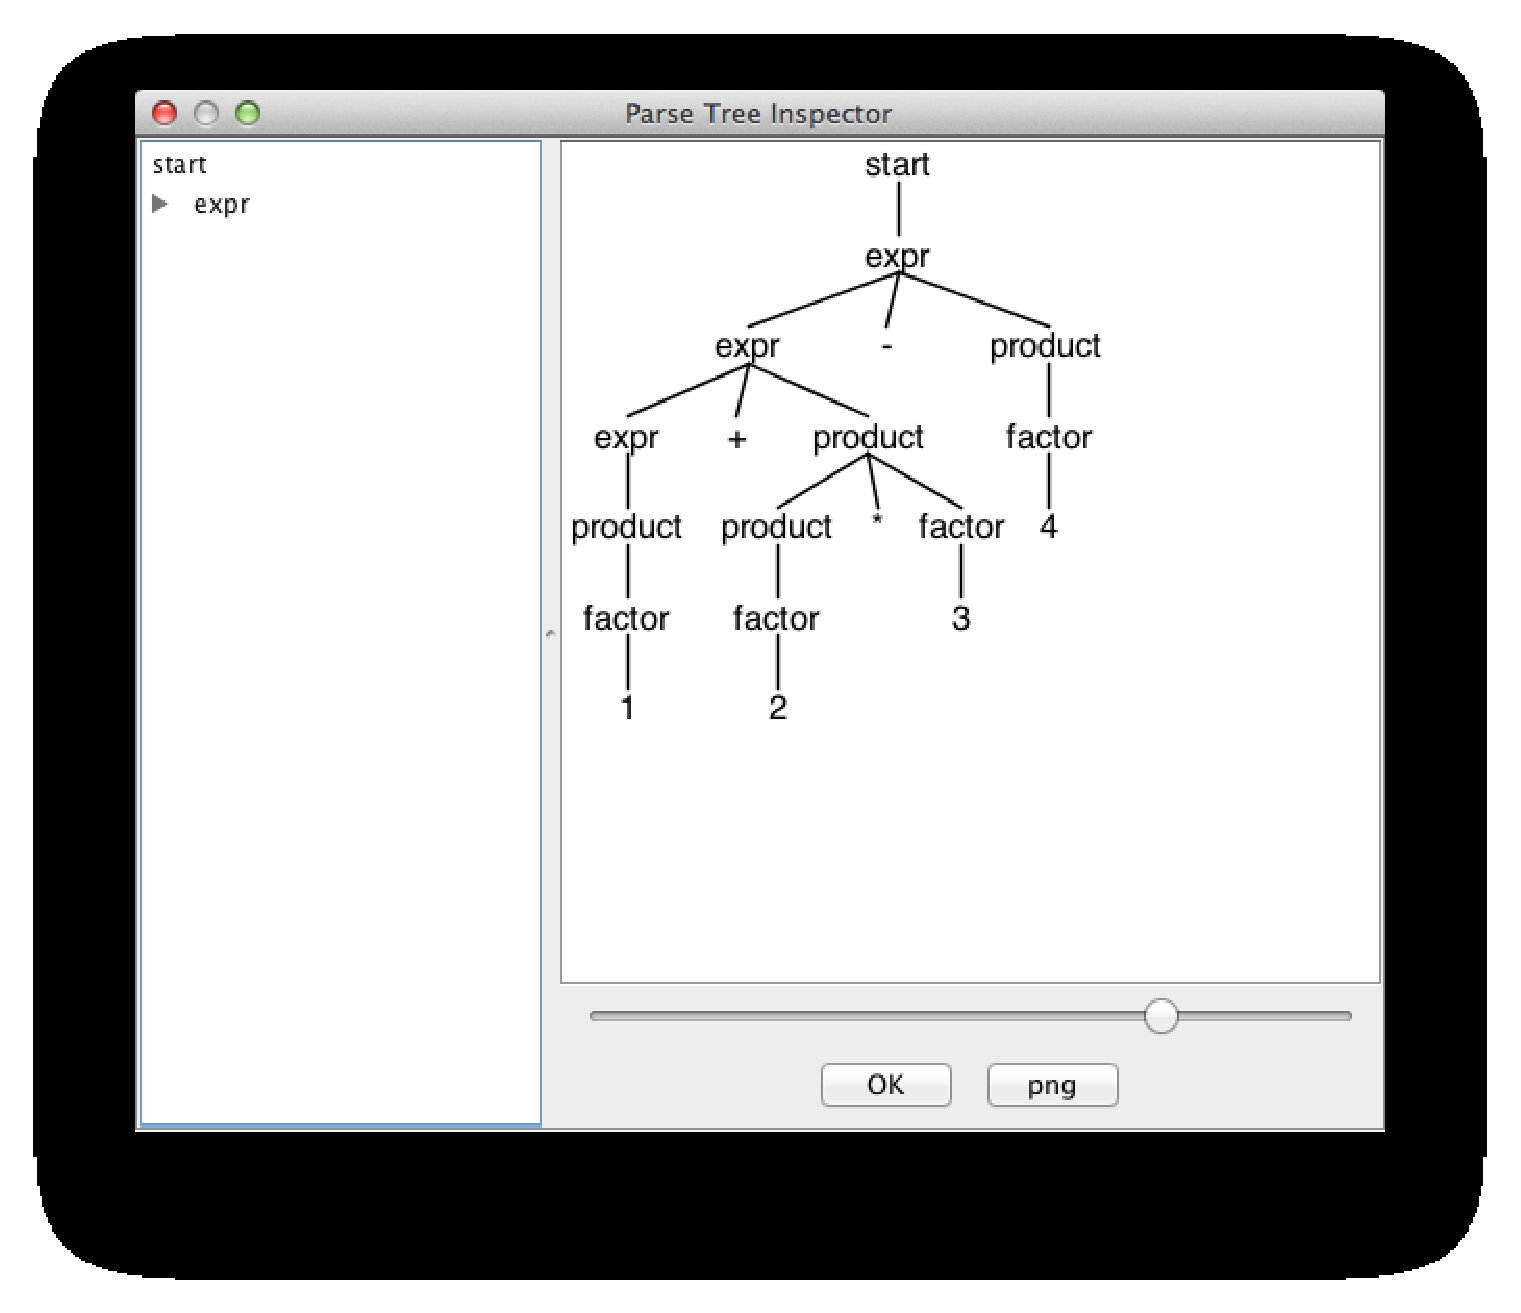
\epsfig{file=Abbildungen/expr.eps, scale=0.7}
   \caption{Syntax-Baum, der beim Parsen des Strings ``\texttt{1+2*3}'' erzeugt wird.}
  \label{fig:expr.eps}
\end{figure}



\section{Ein Parser zur Auswertung arithmetischer Ausdr�cke}
Das letzte Beispiel ist noch nicht sehr spektakul�r, weil die vom Parser erkannten
Ausdr�cke nicht ausgewertet werden.  Wir pr�sentieren jetzt ein komplexeres Beispiel, bei
dem arithmetische Ausdr�cke ausgewertet und die erhaltenen Ergebnisse in Variablen
gespeichert werden k�nnen.  Wir gehen dabei in zwei Schritten vor und pr�sentieren
zun�chst eine reine Grammatik in \textsc{Antlr}-Notation.  Anschlie�end erweitern wir diese
mit Aktionen, in denen die Ausdr�cke ausgewertet werden k�nnen.
Abbildung \ref{fig:Program.g4} zeigt diese Grammatik.  Gegen�ber der vorher gezeigten
Grammatik f�r arithmetische Ausdr�cke gibt es die folgenden �nderungen:

\begin{figure}[!ht]
\centering
\begin{Verbatim}[ frame         = lines, 
                  framesep      = 0.3cm, 
                  labelposition = bottomline,
                  numbers       = left,
                  numbersep     = -0.2cm,
                  xleftmargin   = 0.8cm,
                  xrightmargin  = 0.8cm,
                ]
    grammar Program;
    
    program : stmnt+ ;
    
    stmnt   : ID ':=' expr ';'
            | expr ';'
            ;    
    
    expr    : expr ('+'|'-') product
            | product
            ;
    
    product : product ('*'|'/') factor
            | factor
            ;
    
    factor  : '(' expr ')'
            | ID
            | INT
            ;
    
    ID : [a-zA-Z][a-zA-Z0-9]*;
    INT: '0'|[1-9][0-9]*;
    WS : [ \v\t\n\r] -> skip; 
\end{Verbatim}
\vspace*{-0.3cm}
\caption{Eine Grammatik f�r die Auswertung von Ausdr�cken.}
\label{fig:Program.g4}
\end{figure}


\begin{enumerate}
\item Das Start-Symbol ist jetzt \texttt{program}.  Es steht f�r eine Liste
      von Zuweisungen der folgenden Form:
      \\[0.2cm]
      \hspace*{1.3cm}
      $\textsl{var} \;\mathtt{:=}\; \textsl{expr}\mathtt{;}$
      \\[0.2cm]
      Hier ist \texttt{var} der Name einer Variablen und \textsl{expr} ist ein
      arithmetischer Ausdruck.
\item \texttt{stmnt} bezeichnet eine Zuweisung oder einen einzelnen Ausdruck.
\item Wir haben die Regeln f�r die syntaktischen Variablen \textsl{expr} und \textsl{product}
      vereinfacht, indem wir jeweils die beiden Operatoren ``\texttt{+}'' und ``\texttt{-}'' bzw.
      \squoted{*} und \squoted{/} zusammengefasst haben.
      Da \textsc{Antlr} \textsc{Ebnf}-Grammatiken unterst�tzt, k�nnen wir f�r \textsl{expr}
      beispielsweise die Regel
      \\[0.2cm]
      \hspace*{1.3cm}
      \texttt{expr : expr ('+'|'-') product | product ;}
      \\[0.2cm]
      verwenden.  Die Grammatik-Regel f�r \textsl{product} haben wir in �hnlicher Weise
      ge�ndert.
\item Das Terminal \texttt{ID} bezeichnet den Namen einer Variablen.  Ein solcher Name
      besteht aus einer beliebigen Folge von Buchstaben und Ziffern, die mit einem Buchstaben 
      beginnen muss.
\end{enumerate}
Mit diesem Parser k�nnen wir jetzt zum Beispiel die folgende Eingabe parsen:
\begin{verbatim}
    x = 2 * 3; y = 4 * 5; z = x * x + y * y; 
    z / 3;
\end{verbatim}
Wir wollen nun einen ganz einfachen Interpreter entwickeln, der eine Folge von solchen
Zuweisungen auswertet und die bei der Auswertung berechneten Zwischen-Ergebnisse
in Variablen abspeichert, auf die in folgenden Ausdr�cken Bezug genommen werden kann.
Weiterhin soll jeder Ausdruck, der keiner Variablen zugewiesen wird, ausgewertet und
ausgegeben werden.  Abbildung \ref{fig:Program.g4-2} zeigt die Realisierung eines solchen
Interpreters mit \textsc{Antlr}.

\begin{figure}[!ht]
\centering
\begin{Verbatim}[ frame         = lines, 
                  framesep      = 0.3cm, 
                  labelposition = bottomline,
                  numbers       = left,
                  numbersep     = -0.2cm,
                  xleftmargin   = 0.3cm,
                  xrightmargin  = 0.3cm,
                ]
    grammar Program;
     
    @header {
        import java.util.TreeMap;
    }
    
    @members {
        TreeMap<String, Integer> varTable = new TreeMap<String, Integer>();
    }
    
    program : stmnt+ ;
    
    stmnt : ID ':=' expr ';' { varTable.put($ID.text, $expr.result); }
          |         expr ';' { System.out.println($expr.result);     }
          ;    
    
    expr returns [int result]
        : e = expr { $result = $e.result; }
          (   '+' p = product { $result += $p.result; }
            | '-' p = product { $result -= $p.result; }
          )
        | p = product { $result = $p.result; }
        ;
    
    product returns [int result]
        : p = product { $result = $p.result; }
          (
              '*' f = factor { $result *= $f.result; }
            | '/' f = factor { $result /= $f.result; }
          )
        | f = factor { $result = $f.result; }
        ;
    
    factor returns [int result]
        : '(' expr ')' { $result = $expr.result;           }
        | ID           { $result = varTable.get($ID.text); }
        | INT          { $result = new Integer($INT.text); }
        ;
    
    ID : [a-zA-Z][a-zA-Z0-9]*;
    INT: '0'|[1-9][0-9]*;
    WS : [ \v\t\n\r] -> skip; 
\end{Verbatim} 
%\$
\vspace*{-0.3cm}
\caption{Ein Interpreter zur Auswertung von Ausdr�cken.}
\label{fig:Program.g4-2}
\end{figure}

\begin{enumerate}
\item Da wir die Werte der einzelnen Variablen in einer Tabelle abspeichern m�ssen,
      importieren wir in den Zeilen 3 -- 5 die Klasse \texttt{java.util.TreeMap}, denn
      diese Klasse implementiert Tabellen effizient als bin�re B�ume.

      Allgemein setzt \textsc{Antlr} all den Code, der durch das Schl�sselwort
      ``\texttt{@header}'' spezifiert wird, an den Anfang der erstellten Parser-Datei.
\item In den Zeilen 7 -- 9 definieren wir zus�tzliche Member-Variablen f�r die erzeugte
      Klasse \texttt{ProgramParser}.  In unserem Fall definieren wir hier die Tabelle, die
      sp�ter die Werte der Variablen enth�lt, als Abbildung, die Strings ganze Zahlen zuordnet.

      Allgemein setzt \textsc{Antlr} all den Code, der durch das Schl�sselwort
      ``\texttt{@members}'' spezifiert wird, an den Anfang der erstellten Parser-Klasse.
      Dieses Feature kann sowohl zur Definition von zus�tzlichen Klassen-Variablen als auch
      von Methoden verwendet werden.
      
      Wir reichern nun die Grammatik-Regeln mit Aktionen an, die durchgef�hrt werden, wenn
      der Parser die entsprechende Grammatik-Regel anwendet.  Die Aktionen werden von der
      eigentlichen Grammatik-Regel, f�r die sie angewendet werden sollen, dadurch
      abgesetzt, dass sie in den geschweiften Klammern ``\texttt{\{}'' und ``\texttt{\}}''
      eingefasst werden.
\item Wird vom Parser in Zeile 13 eine Zuweisung der Form $\textsl{var} \;\mathtt{:=}\; \textsl{expr}$
      erkannt,  
      so soll der Wert des Ausdrucks \textsl{expr} berechnet und das Ergebnis in der
      Tabelle \texttt{varTable} unter dem Namen \textsl{var} eingetragen werden.
      In der Grammatik-Regel
      \\[0.2cm]
      \hspace*{1.3cm}
      \textsl{stmnt} $\rightarrow$ \texttt{ID} ':=' \textsl{expr} ';'
      \\[0.2cm]
      haben wir einerseits das Token \texttt{ID}, auf dessen Namen wir mit \texttt{\symbol{36}ID.text}
      zugreifen k�nnen, andererseits haben wir die syntaktische Variable \textsl{expr}.
      Wir werden sp�ter dieser syntaktischen Variable die \textsl{Java}-Variable
      \texttt{result} als Ergebnis-Variable zuordnen, die den zugeh�rigen Wert enth�lt.  
      Dann k�nnen wir mit
      \texttt{\symbol{36}expr.result} auf diesen Wert zugreifen.

      In Zeile 14 haben wir einen einzelnen arithmetischen Ausdruck, den wir auswerten und ausgeben.
\item In Zeile 17 definieren wir mit der Zeile
      \\[0.2cm]
      \hspace*{1.3cm}
      \texttt{expr returns [int result]}
      \\[0.2cm]
      dass die Methode, die eine \textsl{expr} parst, als Ergebnis ein \texttt{int} zur�ck
      gibt und dass dieses in der Variable mit dem Namen \texttt{result} abgespeichert wird.
\item In der Grammatik-Regel
      \\[0.2cm]
      \hspace*{1.3cm}
      \texttt{expr : expr ('+'|'-') product | product ;}
      \\[0.2cm]
      haben wir in Zeile 18 -- 20 den verschiedenen Auftreten der syntaktischen Variablen
      \texttt{expr} und \texttt{product} die Namen $e$ und $p$ zugeordnet, auf die wir dann in den
      Aktionen zugreifen k�nnen.  In den Aktionen muss diesen Variablen allerdings ein Dollar-Zeichen
      vorgestellt werden.

      Die Aktionen selber bestehen nun darin, dass wir der Variablen \texttt{result}
      das Ergebnis der jeweiligen Berechnung zuweisen.
\item In den Zeilen 36 und 37 greifen wir auf die Strings, die den Token
      \texttt{ID} und \texttt{INT} entsprechen, mit Hilfe der f�r Token vordefinierten
      Variable \texttt{text} zur�ck.  Beachten Sie, dass wir in Zeile 36 den Wert, der zu einer
      Variablen in der Tabelle \texttt{varTable} gespeichert ist, auslesen und als Ergebnis zur�ck
      geben. 
\end{enumerate}

\section{Erzeugung abstrakter Syntax-B�ume}
Bei der Auswertung arithmetischer Ausdr�cke im letzten Abschnitt hatten wir Gl�ck
und konnten das Ergebnis eines Ausdrucks unmittelbar mit Hilfe von semantischen Aktionen
berechnen.  Bei komplexeren Problemen ist es in der Regel erforderlich, zun�chst einen
abstrakten Syntax-Baum zu erzeugen.  Die eigentliche Berechnung findet dann erst nach dem
Parsen auf dem Syntax-Baum statt.  Wir wollen dieses Verfahren an einem Beispiel
demonstrieren.  Bei dem Beispiel geht es wieder um die symbolische Differentiation
arithmetischer Ausdr�cke.  Ist beispielsweise der arithmetische Ausdruck 
\[ x \cdot \ln(x) \]
gegeben, so findet sich f�r die Ableitung dieses Ausdrucks nach der Variable $x$ mit Hilfe
der Produkt-Regel das
Ergebnis 
\[ 1 \cdot \ln(x) + x \cdot \frac{1}{x}. \]  
Da die arithmetischen Ausdr�cke nun
zus�tzlich zu den Operatoren, welche die vier Grundrechenarten beschreiben, auch noch 
Funktionszeichen f�r die Exponential-Funktion und den nat�rlichen Logarithmus enthalten
sollen, m�ssen wir die Grammatik aus dem letzten Abschnitt erweitern.
Abbildung \ref{fig:Expr-exp-ln} zeigt die entsprechend erweiterte EBNF-Grammatik.

\begin{figure}[htbp]
  \begin{center}    
  \framebox{
  \framebox{
  \begin{minipage}[t]{9cm}

  \begin{eqnarray*}
  \textsl{expr}   & \rightarrow & \;\textsl{expr}\;\;(\quoted{+}|\quoted{-})  \;\; \textsl{product}  \\
                  & \mid        & \textsl{product}                                 \\[0.2cm]
  \textsl{product} & \rightarrow & \;\textsl{product}\;\;\;\;(\quoted{*}|\quoted{/}) \;\; \textsl{factor} \\
                  & \mid        & \textsl{factor}  \\[0.2cm]
  \textsl{factor} & \rightarrow & \quoted{(} \textsl{expr} \quoted{)}              \\
                  & \mid        & \quoted{exp} \quoted{(} \textsl{expr} \quoted{)} \\
                  & \mid        & \quoted{log} \quoted{(} \textsl{expr} \quoted{)} \\
                  & \mid        & \;\textsc{Variable}                              \\
                  & \mid        & \;\textsc{Number} 
  \end{eqnarray*}
  \vspace*{-0.5cm}

  \end{minipage}}}
  \end{center}
  \caption{EBNF-Grammatik f�r arithmetische Ausdr�cke mit Exponential-Funktion und Logarithmus.}
  \label{fig:Expr-exp-ln}
\end{figure}

\subsection{Implementierung des Parsers}
Abbildung \ref{fig:grammatik.g} zeigt die \textsc{Antlr}-Implementierung der Grammatik
aus Abbildung \ref{fig:Expr-exp-ln}.  

\begin{figure}[!ht]
\centering
\begin{Verbatim}[ frame         = lines, 
                  framesep      = 0.3cm, 
                  labelposition = bottomline,
                  numbers       = left,
                  numbersep     = -0.2cm,
                  xleftmargin   = 0.0cm,
                  xrightmargin  = 0.0cm,
                ]
    grammar Expr;
    
    expr returns [Expr result]
        : e = expr '+' p = product { $result = new Sum(       $e.result, $p.result); }
        | e = expr '-' p = product { $result = new Difference($e.result, $p.result); }
        | p = product              { $result = $p.result; }    
        ;
    
    product returns [Expr result]
        : p = product '*' f = factor { $result = new Product( $p.result, $f.result); }
        | p = product '/' f = factor { $result = new Quotient($p.result, $f.result); }
        | f = factor                 { $result = $f.result; }
        ;
    
    factor returns [Expr result]
        : '(' expr ')'       { $result = $expr.result;                  }
        | 'exp' '(' expr ')' { $result = new Exponential($expr.result); }
        | 'log' '(' expr ')' { $result = new Logarithm(  $expr.result); }
        | VAR                { $result = new Variable($VAR.text);       }
        | NUM                { $result = new Number($NUM.text);         }
        ;
    
    VAR : [a-zA-Z][a-zA-Z0-9]*;
    NUM : '0'|[1-9][0-9]*;
    WS  : [ \v\t\n\r] -> skip; 
\end{Verbatim}
\vspace*{-0.3cm}
\caption{Die \textsc{Antlr}-Spezifikation der Grammatik.}
\label{fig:grammatik.g}
\end{figure}

\begin{enumerate}
\item In Zeile 3 deklarieren wir durch ``\texttt{returns [Expr result]}'',
      dass beim Erkennen einer \textsl{expr} nun ein Objekt der Klasse \texttt{Expr}
      zur�ck gegeben werden soll und dass dieses Objekt �ber den Namen
      \texttt{result} angesprochen werden kann.  Die Klasse \texttt{Expr} ist hier eine abstrakte
      Klasse, von der wir die Klassen
      \begin{enumerate}
      \item \texttt{Sum} (zur Darstellung von Termen der Form $s + t$),
      \item \texttt{Difference} (zur Darstellung von Termen der Form $s - t$),
      \item \texttt{Product} (zur Darstellung von Termen der Form $s * t$),
      \item \texttt{Quotient} (zur Darstellung von Termen der Form $s / t$),
      \item \texttt{Exponential} (zur Darstellung von Termen der Form $\textsl{exp}(s)$),
      \item \texttt{Logarithm} (zur Darstellung von Termen der Form $\textsl{ln}(s)$),
      \item \texttt{Number} (zur Darstellung von Zahlen) und
      \item \texttt{Variable} (zur Darstellung von Variablen)
      \end{enumerate}
      ableiten.  Die Klasse \texttt{Expr} besitzt nur die abstrakte Methode 
      \\[0.2cm]
      \hspace*{1.3cm}
      \texttt{public abstract Expr diff(String x);}
      \\[0.2cm]
      die dazu benutzt wird, einen arithmetischen Ausdruck nach einer gegebenen Variablen
      abzuleiten.  Die von \texttt{Expr} abgeleiteten Klassen sind alle nach dem gleichen Muster
      aufgebaut.  Beispielhaft zeigt Abbildung \ref{fig:Product.java} auf Seite \pageref{fig:Product.java}
        die Implementierung der Klasse 
      \texttt{Product}.
      \begin{enumerate}
      \item Die Klasse beinhaltet die beiden Member-Variablen \texttt{mLhs} und \texttt{mRhs}.
            Ein Objekt der Klasse \texttt{Product} wird als das Produkt
            \\[0.2cm]
            \hspace*{1.3cm}
            $\mathtt{mLhs} * \mathtt{mRhs}$
            \\[0.2cm]
            interpretiert.
      \item Zus�tzlich gibt es eine Implementierung der Methode \texttt{diff}, in der die
            Produkt-Regel umgesetzt wird.
      \item Zur Ausgabe ist weiterhin eine \texttt{toString}-Methode vorhanden.
      \end{enumerate}

\begin{figure}[!ht]
\centering
\begin{Verbatim}[ frame         = lines, 
                  framesep      = 0.3cm, 
                  firstnumber   = 1,
                  labelposition = bottomline,
                  numbers       = left,
                  numbersep     = -0.2cm,
                  xleftmargin   = 0.0cm,
                  xrightmargin  = 0.0cm,
                ]
    public class Product extends Expr {
        private Expr mLhs;
        private Expr mRhs;
    
        public Product(Expr lhs, Expr rhs) {
            mLhs = lhs;
            mRhs = rhs;
        }
        public Expr diff(String x) {
            return new Sum(new Product(mLhs.diff(x), mRhs), new Product(mLhs, mRhs.diff(x)));
        }
        public String toString() {
            return mLhs.toString() + " * " + mRhs.toString();
        }
    }
\end{Verbatim}
\vspace*{-0.3cm}
\caption{Die Klasse \texttt{Product} zur Darstellung von Produkten.}
\label{fig:Product.java}
\end{figure}

      
      
\item In Zeile 4 haben wir zun�chst ein Produkt erkannt, dass wir unter der Variable
      $p$ abspeichern.  Anschlie�end weisen wir der Variable \texttt{result} dieses
      Produkt zu.  Falls nun sp�ter noch ein ``\texttt{+}''-- oder ``\texttt{-}''
      Zeichen gefolgt von einem weiteren Ausdruck gelesen wird, so bauen wir aus dem neu
      gelesenen Ausdruck und dem alten Wert von \texttt{result} den neuen Wert von
      \texttt{result}.  Dies kann mehrmals passieren, da dieser Teil der Grammatik-Regel
      in $( \cdots )*$ eingeschlossen ist.
      
      Beispielsweise wird ein Ausdruck der Form
      \\[0.2cm]
      \hspace*{1.3cm}
      $p_1 + p_2 + p_3$
      \\[0.2cm]
      �bersetzt in ein Java-Objekt der Form
      \\[0.2cm]
      \hspace*{1.3cm}
      $\texttt{new\ Sum}(\texttt{new\ Sum}(p_1, p_2), p_3))$.       
\item Die weiteren Grammatik-Regeln erzeugen in analoger Weise \textsl{Java}-Objekte.
\end{enumerate}

Zum Abschluss zeigt Abbildung \ref{fig:Differentiate.java} noch die Einbindung des Parsers.
Gegen�ber dem in Abbildung \ref{fig:ParseExpr.java} gezeigten Treiber gibt es nur einen
wesentlichen Unterschied: In Zeile 20 wird nun ein Objekt der Klasse \texttt{Expr} erzeugt.
Beachten Sie, dass der Aufruf
\\[0.2cm]
\hspace*{1.3cm}
\texttt{parser.expr()}
\\[0.2cm]
zun�chst ein Objekt der Klasse \texttt{ExprParser.ExprContext} erzeugt.  Bei dieser Klasse handelt
es sich um eine innere Klasse der Klasse \texttt{ExprParser}.  Die innere Klasse
\texttt{ExprContext} enth�lt nun eine Member-Variable mit dem Namen \texttt{result}, in der die
eigentliche \texttt{Expr} gespeichert ist.  
F�r dieses Objekt rufen wir dann in Zeile 21 die Methode $\textsl{diff}()$ auf, welche die
symbolische Ableitung berechnet.


\begin{figure}[!ht]
\centering
\begin{Verbatim}[ frame         = lines, 
                  framesep      = 0.3cm, 
                  labelposition = bottomline,
                  numbers       = left,
                  numbersep     = -0.2cm,
                  xleftmargin   = 0.8cm,
                  xrightmargin  = 0.8cm,
                ]
    import org.antlr.v4.runtime.*;
    import java.io.FileInputStream;
    import java.io.InputStream;
    
    public class Differentiate {
    
        public static void main(String[] args) throws Exception {
            String inputFile = null; 
            if (args.length > 0) { 
    	    inputFile = args[0];
    	}
            InputStream is = System.in;
            if (inputFile != null) {
    	    is = new FileInputStream(inputFile);
    	}
            ANTLRInputStream  input  = new ANTLRInputStream(is);
            ExprLexer         lexer  = new ExprLexer(input);
            CommonTokenStream ts     = new CommonTokenStream(lexer);
            ExprParser        parser = new ExprParser(ts);
            Expr expr = parser.expr().result;
            Expr diff = expr.diff("x");
            System.out.println("d (" + expr + ")/dx = " + diff);
        }
    }
\end{Verbatim}
\vspace*{-0.3cm}
\caption{Ein Treiber f�r den Parser.}
\label{fig:Differentiate.java}
\end{figure}
\pagebreak


\exerciseEng
The \href{https://github.com/karlstroetmann/Formal-Languages}{github directory} associated with this lecture
contains the file
\\[0.2cm]
\hspace*{1.3cm}
\href{https://github.com/karlstroetmann/Formal-Languages/tree/master/Exercises/Grammar2HTML-Antlr/c-grammar.g}{
\texttt{Exercises/Grammar2HTML-Antlr/c-grammar.g}}
\\[0.2cm]
that specifies the syntax of the programming language 
\href{https://en.wikipedia.org/wiki/C_(programming_language)}{\texttt{C}}.

\begin{enumerate}[(a)]
\item Your first task is specify the syntax used to denote the grammar rules given in the file
      \texttt{c-grammar.g}.  Of course, in order to specify this syntax you should use a
      context-free grammar. 
\item Next, you should develop a parser that is capable of reading the file \texttt{c-grammar.g}
      and that, furthermore, can convert this grammar into \textsc{Html}. 
      This parser should be developed using the tool \textsc{Antlr}.
\end{enumerate}

\remarkEng
\begin{enumerate}
\item The directory 
      \\[0.2cm]
      \hspace*{1.3cm}
      \href{https://github.com/karlstroetmann/Formal-Languages/tree/master/Exercises/Grammar2HTML/}{\texttt{Exercises/Grammar2HTML}}
      \\[0.2cm]
      contains several classes that represent various nodes of an abstract syntax tree corresponding to a
      given grammar.  The given classes already contain an implementation of the method $\texttt{toString}()$. This method 
      converts a node of the abstract syntax tree into an \textsc{Html} string.
\item \textsc{Antlr} provides a negation operator that is written as ``\texttt{\symbol{126}}''.
      Using the negation operator comes in handy when recognizing \emph{literal tokens},  
      i.e.~tokens that represent either keywords or operators of the language \texttt{C}.  In the
      file \texttt{c-grammar.g}, literal tokens are enclosed in single quotes.
\item For obscure historical reasons, \textsc{Antlr} treats the string ``\texttt{rule}'' as a 
      keyword.  Therefore, it is not possible to have a syntactical variable that is called
      ``\texttt{rule}''. 
\end{enumerate}



%%% Local Variables: 
%%% mode: latex
%%% TeX-master: "formal-languages"
%%% End: 

\chapter{LL(k)-Sprachen}
In diesem Kapitel werden wir die Theorie vorstellen,  die 
Top-Down Parser-Generatoren wie beispielsweise \textsc{Antlr} zu Grunde liegt.  Es handelt
sich dabei um die Theorie der LL($k$)-Sprachen. 
Dabei steht das erste $L$ daf�r, dass der Parser die Eingabe von \underline{l}inks nach rechts parst,
das zweite $L$ steht daf�r, dass der Parser versucht, eine \underline{L}inks-Ableitung des
zu parsenden Wortes zu berechnen. Eine Links-Ableitung ist dabei eine Ableitung, bei der
immer die linkeste Variable ersetzt wird.
 Die Zahl $k$ in LL($k$) bedeutet, dass der Parser an Hand der n�chsten $k$ Token
entscheidet, welche Regel verwendet wird.  Falls beispielsweise $k=1$ ist, wird also nur das n�chste 
Token zur Entscheidung herangezogen.  Dieses Token bezeichnen wir dann als \emph{Lookahead-Token}.
Wir betrachten zun�chst den Fall $k=1$. 
Bevor wir die Theorie der LL(1)-Parser darstellen, machen wir auf zwei Probleme
aufmerksam, die wir bei der Erstellung von Top-Down-Parsern l�sen m�ssen.
\begin{enumerate}
\item Das erste Problem ist Links-Rekursion, die beispielsweise in den folgenden
      Regeln zur Beschreibung arithmetischer Ausdr�cke auftritt:
      \begin{eqnarray*}
        \textsl{expr}    & \rightarrow & \;\textsl{expr} \quoted{+} \textsl{product}  \\
                         & \mid        & \;\textsl{expr} \quoted{-} \textsl{product}  \\
                         & \mid        & \;\textsl{product}                           
      \end{eqnarray*}
      Wir hatten im Abschnitt \ref{links-rekursion} gezeigt, wie die Links-Rekursion aus
      einer Grammatik eliminiert werden kann. 
      
      Zus�tzlich haben wir gesehen, dass es bei der Verwendung von \textsc{Ebnf}-Grammatiken 
      oft in nat�rlicher Weise m�glich ist, die Links-Rekursion durch die Verwendung der
      Postfix-Operatoren ``\texttt{*}'' und ``\texttt{+}'' zu vermeiden.  Beispielsweise
      k�nnen wir die obigen Regeln f�r arithmetische Ausdr�cke zu der \textsc{Ebnf}-Regel
      \begin{eqnarray*} 
        \textsl{expr}    & \rightarrow & \textsl{product}\;\; ((\quoted{+}|\quoted{-}) \;\;\textsl{product})^* 
      \end{eqnarray*}
      umschreiben.
\item Das zweite Problem erkennen wir, wenn wir die folgende Grammatik-Regel f�r 
      Gleichungen und Ungleichungen betrachten:
      \begin{eqnarray*}
        \textsl{boolExpr} & \rightarrow & \textsl{expr} \quoted{==}    \textsl{expr} \\
                          & \mid        & \textsl{expr} \quoted{<}\;\, \textsl{expr} 
      \end{eqnarray*}
      Diese Grammatik-Regeln sind nicht links-rekursiv, aber
      f�r einen Top-Down-Parser, der mit nur einem Token Look-Ahead
      auskommen soll, ist die Frage, welche der beiden Regeln zum Parsen verwendet
      werden soll, offenbar nicht zu beantworten.  Wir stellen gleich ein Verfahren vor, mit dem sich
      Grammatiken so transformieren lassen, dass dieses Problem verschwindet.
\end{enumerate}

\section{Links-Faktorisierung}
Ist $\textsl{a}$ ein Nicht-Terminal
und gibt es zwei verschiedene Regeln, mit denen $\textsl{a}$ abgeleitet werden kann, beispielsweise
\\[0.2cm]
\hspace*{1.3cm}
$\textsl{a} \rightarrow \beta$ \quad und \quad $\textsl{a} \rightarrow \gamma$,
\\[0.2cm]
so muss es bei der Verwendung eines LL(1)-Parsers m�glich sein, an Hand des Look-Ahead-Tokens zu
erkennen, welche Regel benutzt werden soll.  In der Praxis gibt es h�ufig Situationen, wo
diese Voraussetzung nicht erf�llt ist.  Wir haben oben bereits ein solches Beispiel
gesehen.  Um das Beispiel zu vervollst�ndigen, ben�tigen wir noch Regeln zur Ableitung von
\textsl{expr}.  Abbildung \ref{fig:Expr3} zeigt eine vollst�ndige Grammatik, mit der
Gleichungen und Ungleichungen beschrieben werden k�nnen, die aus arithmetischen Ausdr�cken
aufgebaut sind.


\begin{figure}[htbp]
  \begin{center}    
  \framebox{
  \framebox{
  \begin{minipage}[t]{9cm}

  \begin{eqnarray*}
  \textsl{boolExpr}    & \rightarrow & \textsl{expr} \quoted{==}    \textsl{expr} \\
                       & \mid        & \textsl{expr} \quoted{!=}\;\, \textsl{expr} \\
                       & \mid        & \textsl{expr} \quoted{<=}\;\, \textsl{expr} \\
                       & \mid        & \textsl{expr} \quoted{>=}\;\, \textsl{expr} \\
                       & \mid        & \textsl{expr} \quoted{>}\;\, \textsl{expr} \\
                       & \mid        & \textsl{expr} \quoted{<}\;\, \textsl{expr} \\[0.2cm]
  \textsl{expr}        & \rightarrow & \;\textsl{product}\;\;\textsl{exprRest}            \\[0.2cm]
  \textsl{exprRest}    & \rightarrow & \quoted{+} \textsl{product}\;\;\textsl{exprRest}   \\
                       & \mid        & \quoted{-} \textsl{product}\;\;\textsl{exprRest}   \\
                       & \mid        & \;\varepsilon                                      \\[0.2cm]
  \textsl{product}     & \rightarrow & \;\textsl{factor}\;\;\textsl{productRest}          \\[0.2cm]
  \textsl{productRest} & \rightarrow & \quoted{*} \textsl{factor}\;\;\textsl{productRest} \\
                       & \mid        & \quoted{/} \textsl{factor}\;\;\textsl{productRest} \\
                       & \mid        & \;\varepsilon                                      \\[0.2cm]
  \textsl{factor}      & \rightarrow & \quoted{(} \textsl{expr} \quoted{)}                \\
                       & \mid        & \;\textsc{Number}                                  \\
                       & \mid        & \;\textsc{Identifier} 
  \end{eqnarray*}
  \vspace*{-0.5cm}

  \end{minipage}}}
  \end{center}
  \caption{Grammatik ohne Links-Rekursion f�r Gleichungen und Ungleichungen.}
  \label{fig:Expr3}
\end{figure}

\noindent
Es ist nicht m�glich einen LL(1)-Parser zu implementieren, der Boole'sche Ausdr�cke
mit Hilfe dieser Regeln  erkennen kann, denn alle Regeln f�r \textsl{boolExpr} beginnen
mit \textsl{expr}.  Wir k�nnen die Grammatik aber durch \emph{Links-Faktorisierung}
(Englisch: \emph{left factoring})  
so umschreiben, das ein Token als Look-Ahead ausreicht, indem wir den Teil aus den beiden 
Grammatik-Regeln ausklammern, der am Anfang der beiden Regeln identisch ist.  In dem
obigen Beispiel f�hren wir dann f�r den verbleibenden Rest das neue Nicht-Terminal
\textsl{boolExprRest} ein und erhalten so die Regeln
\begin{eqnarray*}
\textsl{boolExpr}     & \rightarrow & \;\textsl{expr} \;\;\textsl{boolExprRest} \\[0.2cm]
\textsl{boolExprRest} & \rightarrow & \quoted{==}    \textsl{expr} \quad \mid \quad \quoted{!=} \textsl{expr}
                                      \quad \mid \quad \quoted{<=} \textsl{expr}                                  \\
                      & \mid        & \quoted{>=}\;\, \textsl{expr} \quad \mid \quad \quoted{<} \textsl{expr} 
                                      \quad \mid \quad \quoted{>} \textsl{expr}. 
\end{eqnarray*}
Mit diesen Regeln reicht ein Token als Look-Ahead aus, denn die verschiedenen Alternativen f�r 
\mbox{\textsl{boolExprRest}} unterscheiden sich in dem ersten Token des Rumpfs der Regel.
Verwenden wir statt einer einfachen Grammatik eine \textsc{Ebnf}-Grammatik, so lassen sich die 
obigen Regeln k�rzer und klarer in der Form
\begin{eqnarray*}
\textsl{boolExpr} & \rightarrow & \textsl{expr}\;\;
                                  (\quoted{==}\mid \quoted{!=}\mid \quoted{<=} \mid \quoted{>=} \mid \quoted{<})  
                                  \;\;\textsl{expr} 
\end{eqnarray*}
darstellen.

Um den allgemeinen Fall der Links-Faktorisierung diskutieren zu k�nnen, nehmen wir an, dass
$\textsl{a}$ ein Nicht-Terminal ist, das durch insgesamt $m + n$ Regeln definiert wird, wobei der
Rumpf der ersten $m$ Regeln immer mit $\alpha$ anf�ngt, wobei $\alpha$ ein String aus
Terminalen und syntaktischen Variablen ist.  Die Regeln haben also die folgende Form:
\begin{eqnarray*}
  \textsl{a} & \rightarrow & \alpha \;\; \beta_1 \\
    & \mid        & \alpha \;\; \beta_2 \\
    & \vdots      & \vdots              \\
    & \mid        & \alpha \;\; \beta_m \\
    & \mid        & \gamma_1            \\
    & \vdots      & \vdots              \\
    & \mid        & \gamma_n            
\end{eqnarray*}
Bei dieser Darstellung sei vorausgesetzt, dass die Strings $\beta_1$, $\cdots$, $\beta_m$
keinen  Pr�fix haben, der allen $\beta_i$ gemeinsam ist und dass $\alpha$ kein Pr�fix einer der Strings
$\gamma_1, \cdots, \gamma_n$ ist.  Bei der Links-Faktorisierung dieser Regeln klammern wir einerseits den
gemeinsamen Pr�fix $\alpha$ aus und f�hren andererseits eine neue syntaktische Variable $\textsl{b}$ ein, die
den auf $\alpha$ folgenden Rest bezeichnet.  Wir erhalten dann die folgenden Regeln:
\[
\begin{array}{lclclcl}
  \textsl{a} & \rightarrow & \alpha \;\; \textsl{b} & \qquad & \textsl{b} & \rightarrow & \beta_1   \\
    & \mid        & \gamma_1      &        &   & \mid        & \beta_2   \\
    & \vdots      & \vdots        &        &   & \vdots      & \vdots    \\
    & \mid        & \gamma_n      &        &   & \mid        & \beta_m   \\[0.2cm]
\end{array}
\]
Um alle gemeinsamen Pr�fixe auszuklammern muss dieses Verfahren unter 
Umst�nden mehrfach durchgef�hrt werden.  Die n�chste Aufgabe gibt daf�r ein Beispiel.

\exercise
Geben Sie eine Links-Faktorisierung f�r die folgenden Grammatik-Regeln an.
\begin{eqnarray*}
  \textsl{a} & \rightarrow & \quoted{A} \quoted{B} \textsl{u} \quoted{D} \\
             & \mid        & \quoted{A} \textsl{v} \quoted{B} \quoted{D} \\
             & \mid        & \quoted{A} \quoted{B} \textsl{w}            \\
             & \mid        & \quoted{X} \textsl{u}                       \\
             & \mid        & \quoted{X} \textsl{v}                       
\end{eqnarray*}

\solution
Zun�chst eliminieren wir das gemeinsame Pr�fix \qote{A} und f�hren dazu die neue
syntaktische Variable $\textsl{b}$ ein.  Wir erhalten:
\begin{eqnarray*}
  \textsl{a} & \rightarrow & \quoted{A} \textsl{b}             \\
    & \mid        & \quoted{X} \textsl{u}             \\
    & \mid        & \quoted{X} \textsl{v}             \\[0.2cm]
  \textsl{b} & \rightarrow & \quoted{B} \textsl{u} \quoted{D}  \\
    & \mid        & \;\textsl{v} \quoted{B} \quoted{D}\\
    & \mid        & \quoted{B} \textsl{w}             
\end{eqnarray*}
Nun eliminieren wir das Pr�fix \qote{X} aus beiden letzten Regeln f�r $\textsl{a}$.  Wir f�hren
dazu die neue syntaktische Variable $\textsl{c}$ ein. Dann erhalten wir:
\begin{eqnarray*}
  \textsl{a} & \rightarrow & \quoted{A} \textsl{b}              \\
    & \mid        & \quoted{X} \textsl{c}              \\[0.2cm]
  \textsl{c} & \rightarrow & \textsl{u}                         \\
    & \mid        & \textsl{v}                         \\[0.2cm]
  \textsl{b} & \rightarrow & \quoted{B} \textsl{u} \quoted{D}   \\
    & \mid        & \;\textsl{v} \quoted{B} \quoted{D} \\
    & \mid        & \quoted{B} \textsl{w}              
\end{eqnarray*}
Als letztes eliminieren wir das Pr�fix \qote{B}, das in zwei der Regeln f�r die
syntaktische Variable $\textsl{b}$ auftritt.  Wir nennen die neu eingef�hrte Variable $\textsl{d}$ und erhalten:
\begin{eqnarray*}
  \textsl{a} & \rightarrow & \quoted{A} \textsl{b}              \\
    & \mid        & \quoted{X} \textsl{c}              \\[0.2cm]
  \textsl{c} & \rightarrow & \textsl{u}                         \\
    & \mid        & \textsl{v}                         \\[0.2cm]
  \textsl{b} & \rightarrow & \quoted{B} \textsl{d}              \\
    & \mid        & \;\textsl{v} \quoted{B} \quoted{D} \\[0.2cm]
  \textsl{d} & \rightarrow & \textsl{u} \quoted{D}              \\
    & \mid        & \textsl{w}              \hspace*{11cm} _\Box
\end{eqnarray*}
\vspace*{0.3cm}

\noindent
\textbf{Remark}: The parser generator \textsc{Antlr} performs left-factorisation automatically.


\section{\textsl{First} und \textsl{Follow}}
Nicht f�r jede links-faktorisierte Grammatik l�sst sich ein LL(1)-Parser bauen.  Betrachten
wir die folgenden Regeln:
\begin{eqnarray*}
  \textsl{a} & \rightarrow & \textsl{b} \; \mid\; \textsl{c} \\
  \textsl{b} & \rightarrow & \quoted{A} \textsl{u}  \\
  \textsl{c} & \rightarrow & \quoted{A} \textsl{v}  
\end{eqnarray*}
Will der Parser ein $\textsl{a}$ parsen und ist das n�chste Token ein \qote{A}, so ist nicht klar,
ob der Parser als n�chstes die Regel
\\[0.2cm]
\hspace*{1.3cm}
$\textsl{a} \rightarrow \textsl{b}$ \quad oder \quad $\textsl{a} \rightarrow \textsl{c}$
\\[0.2cm]
verwenden soll.  F�r die obige Grammatik l�sst sich daher kein LL(1)-Parser implementieren.
Zur Entscheidung, ob sich f�r eine gegebene Grammatik ein LL(1)-Parser implementieren l�sst,
ben�tigen wir die Funktionen $\textsl{First}()$ und $\textsl{Follow}()$, die wir gleich
definieren werden.  Um diese Funktionen implementieren zu k�nnen, definieren wir vorher  den
Begriff einer $\varepsilon$-erzeugenden syntaktischen Variablen.

\begin{Definition}[$\varepsilon$-erzeugend]
Es sei $G = \langle V, T, R, S \rangle$ eine kontextfreie Grammatik und $\textsl{a}$ sei eine
syntaktische Variable, also $\textsl{a} \in V$.  Die Variable $\textsl{a}$ hei�t 
\emph{$\varepsilon$-erzeugend} genau dann, wenn
\\[0.2cm]
\hspace*{1.3cm}
$\textsl{a} \Rightarrow^* \varepsilon$
\\[0.2cm]
gilt, also dann, wenn sich aus der Variablen $\textsl{a}$ das leere Wort ableiten l�sst. 
Wir schreiben $\textsl{nullable}(\textsl{a})$ wenn die Variable $\textsl{a}$ als $\varepsilon$-erzeugend
nachgewiesen ist.
\eox
\end{Definition}

\examples
\begin{enumerate}
\item Bei der in Abbildung \ref{fig:Expr3} auf Seite \pageref{fig:Expr3} gezeigten Grammatik
      sind offenbar die Variablen \textsl{exprRest} und \textsl{productRest} $\varepsilon$-erzeugend.
\item Wir betrachten nun ein weniger offensichtliches Beispiel.  Die Grammatik $G$
      enthalte die folgenden Regeln:
      \\[0.2cm]
      \hspace*{1.3cm}
      $S \rightarrow \textsl{a} \; \textsl{b} \; \textsl{c}$
      \\[0.2cm]
      \hspace*{1.3cm}
      $\textsl{a} \rightarrow \quoted{X} \textsl{b} \mid \textsl{a} \quoted{Y} \mid \textsl{b}\;\textsl{c}$
      \\[0.2cm]
      \hspace*{1.3cm}
      $\textsl{b} \rightarrow \quoted{X} \textsl{b} \mid \textsl{a} \quoted{Y} \mid \textsl{c}\;\textsl{c}$
      \\[0.2cm]
      \hspace*{1.3cm}
      $\textsl{c} \rightarrow \textsl{a}\;\textsl{b}\; \textsl{c} \mid \varepsilon$
      \\[0.2cm]
      Zun�chst ist offenbar die Variable $\textsl{c}$ $\varepsilon$-erzeugend.  Dann sehen wir,
      dass aufgrund der Regel $\textsl{b} \rightarrow \textsl{c} \;\textsl{c}$ auch $\textsl{b}$ $\varepsilon$-erzeugend ist
      und daraus folgt wegen der Regel $\textsl{a} \rightarrow \textsl{b}\;\textsl{c}$, dass auch $\textsl{a}$
      $\varepsilon$-erzeugend ist.  Schlie�lich erkennen wir $S$ als $\varepsilon$-erzeugend,
      denn die erste Regel lautet
      \\[0.2cm]
      \hspace*{1.3cm}
      $S \rightarrow \textsl{a} \; \textsl{b} \; \textsl{c}$
      \\[0.2cm]
      und hier sind alle Variablen auf der rechten Seite der Regel bereits als
      $\varepsilon$-erzeugende Variablen nachgewiesen worden.
\end{enumerate}
 
\begin{Definition}[$\textsl{First}()$]
Es sei $G = \langle V, T, R, S \rangle$ eine kontextfreie Grammatik und $\textsl{a} \in V$.
Dann definieren wir $\textsl{First}(\textsl{a})$ als die Menge aller der Token $t$, mit denen ein
von $\textsl{a}$ abgeleitetes Wort beginnen kann:
\\[0.2cm]
\hspace*{1.3cm}
$\textsl{First}(\textsl{a}) := \{ t \in T \mid \exists \gamma \in (V \cup T)^*: \textsl{a} \Rightarrow^* t\gamma \}$.
\\[0.2cm]
Die Definition der Funktion $\textsl{First}()$ kann wie folgt auf Strings aus $(V \cup T)^*$ 
erweitert werden: 
\begin{enumerate}
\item $\textsl{First}(\varepsilon) = \{\}$.
\item $\textsl{First}(t \beta) = \{ t \}$ \quad if $t \in T$.
\item $\textsl{First}(\textsl{a} \beta) = \left\{
       \begin{array}[c]{ll}
         \textsl{First}(\textsl{a}) \cup \textsl{First}(\beta) & \mbox{if $\textsl{a} \Rightarrow^* \varepsilon$;} \\
         \textsl{First}(\textsl{a})                            & \mbox{otherwise.}
       \end{array}
       \right.
      $ 
\end{enumerate}
If $\textsl{a}$ is a variable of $G$ and the rules defining $\textsl{a}$ are given as 
\\[0.2cm]
\hspace*{1.3cm}
$\textsl{a} \rightarrow \alpha_1 \mid \cdots \mid \alpha_n$,
\\[0.2cm]
then we have
\\[0.2cm]
\hspace*{1.3cm}
$\textsl{First}(\textsl{a}) = \bigcup\limits_{i=1}^n \textsl{First}(\alpha_i)$.   \eox
\end{Definition}

\remarkEng
Note that the definitions of the function $\textsl{First}(\textsl{a})$ for variables
$\textsl{a} \in V$ and the function $\textsl{First}(\alpha)$ for strings $\alpha \in (V \cup T)^*$
are mutually recursive.  The computation of $\textsl{First}(\textsl{a})$ is best done via a 
fixpoint computation:  Start by setting $\textsl{First}(\textsl{a}) := \{\}$ for all variables $\textsl{a}\in V$ and
then continue to iterate the equations defining $\textsl{First}(\textsl{a})$ until none of the sets
$\textsl{First}(\textsl{a})$ changes any more.  The next example clarifies this idea.

\example
Wir k�nnen f�r die Variablen $\textsl{a}$ der in Abbildung \ref{fig:Expr3} gezeigten Grammatik 
die Mengen $\textsl{First}(\textsl{a})$ iterativ berechnen.  Wir berechnen
die Funktion $\textsl{First}(\textsl{a})$ f�r die einzelnen Variablen $\textsl{a}$ am besten so, dass wir mit den
Variablen beginnen, die in der Hierarchie ganz unten stehen. 
\begin{enumerate}
\item Zun�chst folgt aus den Regeln
      \\[0.2cm]
      \hspace*{1.3cm}
      $\textsl{factor} \rightarrow \quoted{(} \textsl{expr} \quoted{)} \mid \textsc{Number} \mid \textsc{Identifier}$,
      \\[0.2cm]
      dass jeder von \textsl{Factor} abgeleitete String entweder mit einer �ffnenden
      Klammer, einer Zahl oder einem Bezeichner beginnt:
      \\[0.2cm]
      \hspace*{1.3cm}
      $\textsl{First}(\textsl{factor}) = \{ \quoted{(}, \textsc{Number}, \textsc{Identifier}\; \}$.
\item Analog folgt aus den Regeln 
      \\[0.2cm]
      \hspace*{1.3cm}
      $\textsl{productRest} \rightarrow \quoted{*} \textsl{factor}\;\;\textsl{productRest} \;
                            \mid        \quoted{/} \textsl{factor}\;\;\textsl{productRest} \;
                            \mid        \varepsilon$,
      \\[0.2cm]
      dass ein \textsl{productRest} entweder mit dem Zeichen \qote{*} oder \qote{/} beginnt:
      \\[0.2cm]
      \hspace*{1.3cm}
      $\textsl{First}(\textsl{productRest}) = \{ \quoted{*}, \quoted{/} \}$
\item Die Regel f�r die Variable \textsl{product} lautet
      \\[0.2cm]
      \hspace*{1.3cm}
      $\textsl{product} \rightarrow \textsl{factor}\;\;\textsl{productRest}$.
      \\[0.2cm]
      Da die Variable \textsl{factor} nicht $\varepsilon$ erzeugend ist, sehen wir, dass
      die Menge $\textsl{First}(\textsl{product})$ mit der Menge
      $\textsl{First}(\textsl{factor})$ �bereinstimmt:
      \\[0.2cm]
      \hspace*{1.3cm}
      $\textsl{First}(\textsl{product}) = \{ \quoted{(}, \textsc{Number}, \textsc{Identifier}\; \}$.
\item Aus den Regeln
      \\[0.2cm]
      \hspace*{1.3cm}
      $\textsl{exprRest} \rightarrow \quoted{+} \textsl{product}\;\;\textsl{exprRest} 
                         \mid        \quoted{-} \textsl{product}\;\;\textsl{exprRest} 
                         \mid        \varepsilon$
      \\[0.2cm]
      k�nnen wir $\textsl{First}(\textsl{exprRest})$ wie folgt berechnen:
      \\[0.2cm]
      \hspace*{1.3cm}
      $\textsl{First}(\textsl{exprRest}) = \{ \quoted{+}, \quoted{-} \}$.
\item Weiter folgt aus der Regel
      \\[0.2cm]
      \hspace*{1.3cm}
      $\textsl{expr} \rightarrow \textsl{product}\;\;\textsl{exprRest}$
      \\[0.2cm]
      und der Tatsache, dass $\textsl{product}$ nicht $\varepsilon$-erzeugend ist,
      dass die  $\textsl{First}(\textsl{expr})$ mit der Mengen
      $\textsl{First}(\textsl{product})$ �bereinstimmt:
      \\[0.2cm]
      \hspace*{1.3cm}
      $\textsl{First}(\textsl{expr}) = \{ \quoted{(}, \textsc{Number}, \textsc{Identifier}\; \}$.
\item Schlie�lich folgt aus den Regeln f�r die syntaktische Variable \textsl{boolExpr}
      sowie der Tatsache, dass die syntaktische Variable \textsl{expr} nicht $\varepsilon$-erzeugend ist,
      dass $\textsl{First}(\textsl{boolExpr})$ mit $\textsl{First}(\textsl{expr})$ identisch ist:
      \\[0.2cm]
      \hspace*{1.3cm}
      $\textsl{First}(\textsl{boolExpr}) = \{ \quoted{(}, \textsc{Number}, \textsc{Identifier}\; \}$.
\end{enumerate}
Since we have computed the sets $\textsl{First}(\textsl{a})$ in a clever order, we did not have to perform a
proper fixpoint iteration in this example.
\eox


\begin{Definition}[$\textsl{Follow}()$]
Es sei $G = \langle V, T, R, S \rangle$ eine kontextfreie Grammatik und $\textsl{a} \in V$.
Bei der Berechnung von $\textsl{Follow}()$ wird die Grammatik zun�chst abge�ndert,
indem wir das Symbol \qote{\symbol{36}} als neues Symbol zu der Menge $T$ der Terminale
hinzuf�gen.  Zu den Variablen wird das neue Symbol $\widehat{S}$ hinzugef�gt, das auch
gleichzeitig das neue Start-Symbol der Grammatik ist.  Zu der Menge $R$ der Regeln
f�gen wir die folgende Regel neu hinzu:
\\[0.2cm]
\hspace*{1.3cm}
$\widehat{S} \rightarrow S \quoted{\symbol{36}}$.
\\[0.2cm]
Das Terminal \qote{\symbol{36}} steht hierbei f�r das Ende der Eingabe (\textsc{Eof},
\emph{end of file}).
Weiter definieren wir
\\[0.2cm]
\hspace*{1.3cm}
 $\widehat{T} := T \cup \{ \quoted{\symbol{36}} \}$.
\\[0.2cm]
Die so ver�nderte Grammatik bezeichnen wir als die \emph{augmentierte} Grammatik.
Dann definieren wir $\textsl{Follow}(\textsl{a})$ als die Menge aller der Token $t$, die in einer
Ableitung auf $\textsl{a}$ folgen k�nnen:
\\[0.2cm]
\hspace*{1.3cm}
$\textsl{Follow}(\textsl{a}) := 
 \{ t \in \widehat{T} \mid \exists \beta,\gamma \in (V \cup \widehat{T})^*: 
                           \widehat{S} \Rightarrow^* \beta \textsl{a} t \gamma 
  \}
$.
\\[0.2cm]
Wenn sich aus dem Start-Symbol $\widehat{S}$ also irgendwie ein String $\beta \textsl{a} t\gamma$ ableiten l�sst,
bei dem das Token $t$ auf die Variable $\textsl{a}$ folgt, dann ist $t$ ein Element
der Menge $\textsl{Follow}(\textsl{a})$.
\eox
\end{Definition}

\example
Wir untersuchen wieder die in Abbildung \ref{fig:Expr3} gezeigte Grammatik f�r arithmetische Ausdr�cke.
\begin{enumerate}
\item Aufgrund der neu hinzugef�gten Regel
      \\[0.2cm]
      \hspace*{1.3cm}
      $\widehat{S} \rightarrow \textsl{boolExpr} \quoted{\symbol{36}}$
      \\[0.2cm]
      muss die Menge $\textsl{Follow}(\textsl{boolExpr})$ das Zeichen \qote{\symbol{36}}
      enthalten.  Da die syntaktische Variable \textsl{boolExpr} sonst nirgends in der
      Grammatik vorkommt, haben wir 
      \\[0.2cm]
      \hspace*{1.3cm}
      $\textsl{Follow}(\textsl{boolExpr}) = \{ \quoted{\symbol{36}} \}$.
\item Die Grammatik-Regeln f�r die syntaktische Variable \textsl{boolExpr}
      zeigen uns zun�chst, dass die Menge $\textsl{Follow}(\textsl{expr})$ die Zeichen
      \qote{==}, \qote{!=}, \qote{<=}, \qote{>=}, \qote{<}   und \qote{>} enth�lt.  Da \textsl{expr} auch am Ende dieser Regeln steht,
      folgt weiter, dass alle Elemente aus $\textsl{Follow}(\textsl{boolExpr})$ auch auf 
      \textsl{expr} folgen k�nnen, wir haben also auch
      \\[0.2cm]
      \hspace*{1.3cm}
      $\quoted{\symbol{36}} \in \textsl{Follow}(\textsl{expr})$.
      \\[0.2cm]
      Aufgrund der Regel 
      \\[0.2cm]
      \hspace*{1.3cm}
      $\textsl{factor} \rightarrow \quoted{(} \textsl{expr} \quoted{)}$
      \\[0.2cm]
      muss die Menge $\textsl{Follow}(\textsl{expr})$ au�erdem das Zeichen \qote{)}
      enthalten.  Also haben wir insgesamt
      \\[0.2cm]
      \hspace*{1.3cm}
      $\textsl{Follow}(\textsl{expr}) = \{ \quoted{==}, \quoted{!=}, \quoted{>=}, \quoted{<=}, \quoted{>}, \quoted{<}, \quoted{\symbol{36}}, \quoted{)} \}$.
\item Aufgrund der Regel 
      \\[0.2cm]
      \hspace*{1.3cm}
      $\textsl{expr} \rightarrow \textsl{product}\;\;\textsl{exprRest}$
      \\[0.2cm]      
      wissen wir, dass alle Terminale, die auf ein \textsl{expr} folgen k�nnen, auch auf
      ein \textsl{exprRest} folgen k�nnen, womit wir schon mal wissen, dass
      $\textsl{Follow}(\textsl{exprRest})$ die Token \qote{==}, \qote{!=}, \qote{<=}, \qote{>=}, \qote{<}, \qote{\symbol{36}}  und \qote{)}
      enth�lt.   Da \textsl{exprRest} sonst nur am Ende der Regeln vorkommt, die
      \textsl{exprRest} definieren, sind das auch schon alle Token, die auf
      \textsl{exprRest} folgen k�nnen und wir haben
      \\[0.2cm]
      \hspace*{1.3cm}
      $\textsl{Follow}(\textsl{exprRest}) = 
       \{ \quoted{==}, \quoted{!=}, \quoted{>=}, \quoted{<=}, \quoted{>}, \quoted{<}, \quoted{\symbol{36}}, \quoted{)} \}$.
\item Die Regeln 
      \\[0.2cm]
      \hspace*{1.3cm}
      $\textsl{exprRest} \rightarrow \quoted{+} \textsl{product}\;\;\textsl{exprRest} 
                         \mid        \quoted{-} \textsl{product}\;\;\textsl{exprRest}$
      \\[0.2cm]
      zeigen, dass auf ein \textsl{product} alle Elemente aus $\textsl{First}(\textsl{exprRest})$
      folgen k�nnen, aber das ist noch nicht alles:  Da die Variable \textsl{exprRest}
      $\varepsilon$-erzeugend ist, k�nnen zus�tzlich auf \textsl{product} auch
      alle Token folgen, die auf \textsl{exprRest} folgen.  Damit haben wir insgesamt
      \\[0.2cm]
      \hspace*{1.3cm}
      $\textsl{Follow}(\textsl{product}) = 
      \{ \quoted{+}, \quoted{-},  \quoted{==}, \quoted{!=}, \quoted{>=}, \quoted{<=}, \quoted{>}, \quoted{<}, \quoted{\symbol{36}}, \quoted{)} \}$.
\item Die Regel
      \\[0.2cm]
      \hspace*{1.3cm}
      $\textsl{product} \rightarrow \textsl{factor}\;\;\textsl{productRest}$
      \\[0.2cm]      
      zeigt, dass alle Terminale, die auf ein \textsl{product} folgen k�nnen, auch auf
      ein \textsl{productRest} folgen k�nnen.
      Da \textsl{productRest} sonst nur am Ende der Regeln vorkommt, die
      \textsl{productRest} definieren, sind das auch schon alle Token, die auf
      \textsl{productRest} folgen k�nnen und wir haben insgesamt
      \\[0.2cm]
      \hspace*{1.3cm}
      $\textsl{Follow}(\textsl{productRest}) = 
      \{ \quoted{+}, \quoted{-}, \quoted{==}, \quoted{!=}, \quoted{>=}, \quoted{<=}, \quoted{>}, \quoted{<}, \quoted{\symbol{36}}, \quoted{)} \}$.
\item Die Regeln 
      \\[0.2cm]
      \hspace*{1.3cm}
      $\textsl{productRest} \rightarrow \quoted{*} \textsl{factor}\;\;\textsl{productRest} 
                            \mid        \quoted{/} \textsl{factor}\;\;\textsl{productRest}$ 
      \\[0.2cm]
      zeigen, dass auf ein \textsl{factor} alle Elemente aus $\textsl{First}(\textsl{productRest})$
      folgen k�nnen, aber das ist noch nicht alles:  Da die Variable \textsl{productRest}
      $\varepsilon$-erzeugend ist, k�nnen zus�tzlich auf \textsl{factor} auch
      alle Token folgen, die auf \textsl{productRest} folgen.  Damit haben wir insgesamt
      \\[0.2cm]
      \hspace*{1.3cm}
      $\textsl{Follow}(\textsl{factor}) = 
      \{ \quoted{*}, \quoted{/}, \quoted{+}, \quoted{-}, \quoted{==}, \quoted{!=}, \quoted{>=}, \quoted{<=}, \quoted{>}, \quoted{<}, \quoted{\symbol{36}}, \quoted{)} \}$.
      \qed
\end{enumerate}

\noindent
Das letzte Beispiel zeigt, dass die Berechnung des Pr�dikats $\textsl{nullable}()$ 
und die Berechnung der Mengen $\textsl{First}(\textsl{a})$ und $\textsl{Follow}(\textsl{a})$ f�r eine syntaktische
Variable $\textsl{a}$ eng miteinander verbunden sind.  
Es sei
\\[0.2cm]
\hspace*{1.3cm}
 $\textsl{a} \rightarrow Y_1 Y_2 \cdots Y_k$ 
\\[0.2cm]
eine Grammatik-Regel.
Dann bestehen zwischen dem Pr�dikat $\texttt{nullable}()$ und den beiden Funktionen
$\textsl{First}()$ und $\textsl{Follow}()$ die folgenden Beziehungen:
\begin{enumerate}
\item $\forall t \in T: \neg\, \textsl{nullable}(t)$.
\item $k = 0 \Rightarrow \textsl{nullable}(\textsl{a})$.
\item $\bigl(\forall i \in \{1, \cdots, k\}: \textsl{nullable}(Y_i)\bigr) \Rightarrow
       \textsl{nullable}(\textsl{a})$.

      Setzen wir hier $k=0$ so sehen wir, dass 2.~ein Spezialfall von 3.~ist.
\item $\textsl{First}(Y_1) \subseteq \textsl{First}(\textsl{a})$.
\item $\bigl(\forall j \in \{1,\cdots,i-1\}: \textsl{nullable}(Y_j)\bigr) \Rightarrow
       \textsl{First}(Y_i) \subseteq \textsl{First}(\textsl{a})$.

       Setzen wir oben $i=1$, so sehen wir, dass 4.~ein Spezialfall von 5.~ist.
\item $\textsl{Follow}(\textsl{a}) \subseteq \textsl{Follow}(Y_k)$.
\item $\bigl(\forall j \in \{i+1, \cdots, k\}: \textsl{nullable}(Y_j)\bigr) \Rightarrow 
       \textsl{Follow}(\textsl{a}) \subseteq \textsl{Follow}(Y_i)$.

      Setzen wir hier $i=k$ so sehen wir, dass 6.~ein Spezialfall von 7.~ist.
\item $\forall i \in \{1,\cdots,k-1\}:\textsl{First}(Y_{i+1}) \subseteq \textsl{Follow}(Y_i)$.
\item $\bigl(\forall j \in \{i+1, \cdots, l-1\}: \textsl{nullable}(Y_j)\bigr) \Rightarrow 
       \textsl{First}(Y_l) \subseteq \textsl{Follow}(Y_i)$.

      Setzen wir hier $l=i+1$ so sehen wir, dass 8.~ein Spezialfall von 9.~ist.
\end{enumerate}
Mit Hilfe dieser Beziehungen k�nnen $\textsl{nullable}()$, $\textsl{First}()$ und
$\textsl{Follow}()$ iterativ �ber eine Fixpunkt-Iteration berechnet werden:  
\begin{enumerate}
\item Zun�chst werden die Funktionen $\textsl{First}(\textsl{a})$ und
      $\textsl{Follow}(\textsl{a})$ f�r jede syntaktische Variable $\textsl{a}$ mit der leeren Menge initialisiert.
      Das Pr�dikat $\textsl{nullable}(\textsl{a})$ wird f�r jede syntaktische Variable auf $\texttt{false}$
      gesetzt.
\item Anschlie�end werden die oben angegebenen Regeln so lange angewendet, wie sich durch die
      Anwendung �nderungen ergeben. 
\end{enumerate}

\section{LL(1)-Grammatiken}
Wir k�nnen nun die Frage beantworten, f�r welche Grammatiken ein Top-Down-Parser erzeugt
werden kann, der immer mit einem Token Lookahead auskommt.  

\begin{Definition}[LL(1)-Grammatik]
Eine Grammatik $G$ ist eine \emph{LL(1)-Grammatik} genau dann, wenn f�r jede syntaktische Variable
$\textsl{a}$, f�r die es in der Grammatik $G$ zwei verschiedene Regeln
\\[0.2cm]
\hspace*{1.3cm}
$\textsl{a} \rightarrow \alpha$ \quad und \quad $\textsl{a} \rightarrow \beta$ 
\\[0.2cm]
gibt, die folgenden Bedingungen erf�llt sind:
\begin{enumerate}
\item $\neg( \alpha \Rightarrow^* \varepsilon \wedge \beta \Rightarrow^* \varepsilon)$.

      Die R�mpfe zweier verschiedener Regeln derselben Variablen
      d�rfen nicht beide das leere Wort ableiten.
\item $\textsl{First}(\alpha) \cap \textsl{First}(\beta) = \{\}$.

      Die Ableitungen der R�mpfe zweier verschiedener Regeln derselben Variablen
      d�rfen nicht mit dem selben Token beginnen.
\item   $(\beta  \Rightarrow^* \varepsilon) \rightarrow \textsl{First}(\alpha) \cap
\textsl{Follow}(\textsl{a}) = \{\}$.

      Wenn $\beta$ den leeren String ableitet, dann m�ssen die Mengen
      $\textsl{First}(\alpha)$ und $\textsl{Follow}(\textsl{a})$ disjunkt sein.  
      \eox
\end{enumerate}
\end{Definition}

\noindent
Wir diskutieren nun die Idee, die hinter der obigen Definition steht.
\begin{enumerate}
\item Falls das leere Wort sowohl �ber die Regel
      \\[0.2cm]
      \hspace*{1.3cm}
      $\textsl{a} \rightarrow \alpha$ \quad als auch �ber \quad $\textsl{a} \rightarrow \beta$
      \\[0.2cm]
      ableitbar w�re, so wissen wir nicht, welche Regel wir anwenden sollen, wenn
      wir ein $\textsl{a}$ ableiten sollen und das n�chste Eingabe-Token ein Element der Menge
      $\textsl{Follow}(\textsl{a})$ ist.
\item Um ein $\textsl{a}$ zu parsen und zwischen den beiden Regeln f�r $\textsl{a}$ unterscheiden zu k�nnen,
      verwenden wir das folgende Rezept:

      Parsen wir ein $\textsl{a}$ und ist das Lookahead-Token ein Element der Menge
      $\textsl{First}(\alpha)$, so verwenden wir die Regel
      \\[0.2cm]
      \hspace*{1.3cm}
      $\textsl{a} \rightarrow \alpha$.
      \\[0.2cm]
      Analog verwenden wir die Regel
      \\[0.2cm]
      \hspace*{1.3cm}
      $\textsl{a} \rightarrow \beta$,
      \\[0.2cm]
      wenn das Lookahead-Token ein Element der Menge $\textsl{First}(\beta)$ ist.

      Dieses Rezept funktioniert nat�rlich nur, wenn die Mengen $\textsl{First}(\alpha)$
      und $\textsl{First}(\beta)$ disjunkt sind.
\item Das obige Rezept um ein $\textsl{a}$ zu parsen muss in dem Fall, dass $\beta$ das leere Wort
      ableitet, wie folgt erweitert werden.
  
      Gilt $\beta \Rightarrow^* \varepsilon$ und ist das Lookahead-Token ein Element der
      Menge $\textsl{Follow}(\textsl{a})$, so verwenden wir die Regel
      \\[0.2cm]
      \hspace*{1.3cm}
      $\textsl{a} \rightarrow \beta$.
     
      Damit diese Regel nicht im Widerspruch zu den unter Punkt 2.~genannten Regeln steht,
      ben�tigen wir die Bedingungen
      \\[0.2cm]
      \hspace*{1.3cm}
      $(\beta  \Rightarrow^* \varepsilon) \rightarrow \textsl{First}(\alpha) \cap \textsl{Follow}(\textsl{a}) = \{\}.$ 
\end{enumerate}
Insgesamt versuchen wir also dann mit einer Regel $\textsl{a} \rightarrow \alpha$ zu reduzieren,
wenn eine der beiden folgenden Bedingungen erf�llt sind.  In diesen Bedingungen bezeichnet
\textsl{lat} das Lookahead-Token.
\begin{enumerate}
\item $\textsl{lat} \in \textsl{First}(\alpha)$ \quad oder
\item $\alpha \Rightarrow^* \varepsilon$ und $\textsl{lat} \in \textsl{Follow}(\alpha)$.
\end{enumerate}

\remark
Falls eine Grammatik $G$ links-rekursiv ist und die links-rekursiven Regeln nicht 
�berfl�ssig sind, dann ist klar, dass $G$ keine LL(1)-Grammatik sein kann.


\subsection{Berechnung der Parse-Tabelle}
Nach diesen Vorbereitungen k�nnen wir nun zu einer LL(1)-Grammatik die \emph{Parse-Tabelle}
berechnen.  F�r eine Grammatik $G = \langle V, T, R, S \rangle$ ist die Parse-Tabelle
\\[0.2cm]
\hspace*{1.3cm}
$\textsl{parseTable}: V \times T \rightarrow 2^R$,
\\[0.2cm]
eine Funktion, so dass der Aufruf $\textsl{parseTable}(\textsl{a},t)$ einer syntaktischen Variable $\textsl{a}$ und
einem Token $t$ die Menge aller Regeln der Form  
\\[0.2cm]
\hspace*{1.3cm}
$\textsl{a} \rightarrow \alpha$
\\[0.2cm]
zuordnet, die bei einer Ableitung von $\textsl{a}$ in Frage kommen, wenn das n�chste zu lesenden Token den
Wert $t$ hat.  Diese Funktion gen�gt den folgenden beiden Bedingungen:
\begin{enumerate}
\item Ist  $\textsl{a} \rightarrow \alpha$ eine Regel der Grammatik und ist $t$ ein Token aus der Menge 
      $\textsl{First}(\alpha)$, dann ist diese Regel ein Element der Menge
      $\textsl{parseTable}(\textsl{a},t)$:
      \\[0.2cm]
      \hspace*{1.3cm}
      $(\textsl{a} \rightarrow \alpha) \in R \; \wedge \; t \in \textsl{First}(\alpha) 
      \;\Rightarrow\; (\textsl{a} \rightarrow \alpha) \in \textsl{parseTable}(\textsl{a},t)$.
\item Ist $\textsl{a} \rightarrow \alpha$ eine Regel der Grammatik, wobei $\alpha$ 
      $\varepsilon$-erzeugend ist, und ist $t$ ein Token aus der Menge 
      $\textsl{Follow}(\textsl{a})$, dann ist diese Regel ein Element der Menge
      $\textsl{parseTable}(\textsl{a},t)$:
      \\[0.2cm]
      \hspace*{1.3cm}
      $(\textsl{a} \rightarrow \alpha) \in R \; \wedge \; \alpha \Rightarrow^* \varepsilon 
       \;\wedge\;t \in \textsl{Follow}(\textsl{a}) 
       \;\Rightarrow\; (\textsl{a} \rightarrow \alpha) \in \textsl{parseTable}(\textsl{a},t)$.
\end{enumerate}
Eine Grammatik ist genau dann eine $LL(1)$-Grammatik, wenn die Mengen
$\textsl{parseTable}(\textsl{a},t)$ f�r jede syntaktische Variable $\textsl{a}$ und jedes Token $t$ maximal
eine Regel enth�lt:
\\[0.2cm]
\hspace*{1.3cm} $G$ ist LL(1) \quad g.d.w. \quad  
$\forall \textsl{a} \in V: \forall t \in T: \textsl{card}\bigl(\textsl{parseTable}(\textsl{a},t)\bigr) \leq 1$.
\\[0.2cm]
Falls die Menge $\textsl{parseTable}(\textsl{a},t)$ leer ist, so hei�t dies einfach, dass wir beim
Parsen von $\textsl{a}$ nicht auf das Token $t$ sto�en k�nnen.  Parsen wir also ein $\textsl{a}$ und sehen
als erstes Zeichen das Token $t$, so muss ein Syntax-Fehler vorliegen.  

\section{LL(k)-Grammatiken}

\begin{figure}[!ht]
  \begin{center}    
  \framebox{
  \framebox{
  \begin{minipage}[t]{9cm}

  \begin{eqnarray*}
  \textsl{expr}        & \rightarrow & \;\textsl{product}\;\;\textsl{exprRest}            \\[0.2cm]
  \textsl{exprRest}    & \rightarrow & \quoted{+} \textsl{product}\;\;\textsl{exprRest}   \\
                       & \mid        & \quoted{-} \textsl{product}\;\;\textsl{exprRest}   \\
                       & \mid        & \;\varepsilon                                      \\[0.2cm]
  \textsl{product}     & \rightarrow & \;\textsl{factor}\;\;\textsl{productRest}          \\[0.2cm]
  \textsl{productRest} & \rightarrow & \quoted{*} \textsl{factor}\;\;\textsl{productRest} \\
                       & \mid        & \quoted{/} \textsl{factor}\;\;\textsl{productRest} \\
                       & \mid        & \;\varepsilon                                      \\[0.2cm]
  \textsl{factor}      & \rightarrow & \quoted{(} \textsl{expr} \quoted{)}                \\
                       & \mid        & \;\textsl{Number}                                  \\
                       & \mid        & \;\textsc{Identifier}                              \\
                       & \mid        & \;\textsc{Identifier} \quoted{(} \textsl{argList} \quoted{)}
                       \\[0.2cm]
  \textsl{argList}     & \rightarrow & \textsl{expr} \;\;\textsl{argsRest}                    \\
                       & \mid        & \;\varepsilon                                      \\[0.2cm]
  \textsl{argsRest}    & \rightarrow & \quoted{,} \textsl{expr} \;\;\textsl{argsRest}         \\
                       & \mid        & \varepsilon                   
  \end{eqnarray*}
  \vspace*{-0.5cm}

  \end{minipage}}}
  \end{center}
  \caption{Arithmetische Ausdr�cke mit Funktions-Aufrufen.}
  \label{fig:Expr4}
\end{figure}

\noindent
Viele interessante Grammatiken sind keine $LL(1)$-Grammatiken.
Abbildung \ref{fig:Expr4} zeigt ein Beispiel.  Bei dieser Grammatiken werden f�r arithmetische
Ausdr�cke auch Funktionsaufrufe der Form
\\[0.2cm]
\hspace*{1.3cm}
$f(a_1, \cdots, a_n)$
\\[0.2cm]
zugelassen.  Dabei ist $f$ ein Funktionszeichen, das syntaktisch nicht von einem Identfier zu
unterscheiden ist.  Dadurch gibt es zwischen den beiden Regeln
\\[0.2cm]
\hspace*{1.3cm}
$\textsl{factor} \rightarrow \textsc{Identifier}$ \quad und \quad
$\textsl{factor} \rightarrow \textsc{Identifier} \quoted{(} \textsl{argList} \quoted{)}$ 
\\[0.2cm]
einen Konflikt:  Soll ein \textsl{factor} geparst werden und ist das n�chste zu lesende Zeichen ein 
\textsc{Identifier}, so ist nicht klar, welche der beiden Regeln angewendet werden sollen.
Es gibt hier zwei m�gliche L�sungen:  Einerseits k�nnten wir die Grammatik durch eine
Links-Faktorisierung umschreiben.  Andererseits ist es auch m�glich, das Problem dadurch zu l�sen,
das wir bei der Entscheidung, welche der Grammatik-Regeln verwendet werden soll, zus�tzlich das
zweite Zeichen zu ber�cksichtigen:  Handelt es sich dabei um das Zeichen $\quoted{(}$, so ist offenbar die Regel
\\[0.2cm]
\hspace*{1.3cm}
$\textsl{factor} \rightarrow \textsc{Identifier} \quoted{(} \textsl{argList} \quoted{)}$ 
\\[0.2cm]
heranzuziehen, andernfalls muss die Regel
\\[0.2cm]
\hspace*{1.3cm}
$\textsl{factor} \rightarrow \textsc{Identifier}$ 
\\[0.2cm]
verwendet werden.

Im allgemeinen Fall kann das Verfahren so erweitert werden, dass $k$ Token bei der Entscheidung,
welche Regel zu verwenden ist, als Lookahead herangezogen werden.  
Wir skizzieren die Grundz�ge dieser Theorie.
Als erstes verallgemeinern wir die Definition der Funktion $\textsl{First}()$.  

\begin{Definition}[$\textsl{First}(k,\alpha)$]
  Es sei $G = \langle V, T, R, S \rangle$ eine kontextfreie Grammatik. Wir definieren eine Funktion
  \\[0.2cm]
  \hspace*{1.3cm}
  $\textsl{First}: \mathbb{N} \times (V \cup T)^* \rightarrow 2^{T^*}$,
  \\[0.2cm]
  so dass $\textsl{First}(k,\alpha)$ f�r eine nat�rliche Zahl $k$ und einen String $\alpha$, der aus
  Terminalen und syntaktischen Variablen besteht, die Menge der Token-Strings berechnet, die
  h�chstens die L�nge $k$ haben und die Pr�fix eines von $\alpha$ abgeleiteten Strings sind.  Formal
  lautet die Definition:
  \\[0.2cm]
  \hspace*{1.3cm}
  $\textsl{First}(k, \alpha) := 
  \bigl\{ x \in T^* \mid \exists y \in T^*: \alpha \Rightarrow^* x y \wedge |x| = k \} \cup
  \{ x \in T^* \mid \alpha \Rightarrow^* x \wedge |x| < k \bigr\}.$ \eox
\end{Definition}

\example
Abbildung \ref{fig:expr-id.g} zeigt eine Grammatik f�r arithmetische Ausdr�cke.
Berechnen wir f�r die in dieser Grammatik auftretenden Variablen $v$ die Mengen
$\textsl{First}(2,v)$, so erhalten wir beispielsweise:
\begin{enumerate}
\item $\textsl{First}(2, \textsl{expr}) = 
      \bigl\{\, \textsc{Id}, \,\squoted{(}\, \textsc{Id},\, \squoted{((},\,
      \textsc{Id} \squoted{+},\, \textsc{Id} \squoted{-},\,
      \textsc{Id} \squoted{*},\, \textsc{Id} \squoted{/}\,
      \bigr\}$,
\item $\textsl{First}(2, \textsl{product}) = 
      \bigl\{\, \textsc{Id}, \,\squoted{(}\, \textsc{Id},\, \squoted{((},\,
      \textsc{Id} \squoted{*},\, \textsc{Id} \squoted{/}\,
      \bigr\}$,
\item $\textsl{First}(2, \textsl{factor}) = 
      \bigl\{\, \textsc{Id}, \,\squoted{(}\, \textsc{Id},\, \squoted{((}\,
      \bigr\}$.
\end{enumerate}


\begin{figure}[htbp]
  \begin{center}    
  \framebox{
  \framebox{
  \begin{minipage}[t]{9cm}

  \begin{eqnarray*}
  \textsl{expr}        & \rightarrow & \textsl{expr} \quoted{+} \textsl{product}        \\
                       & \mid        & \textsl{expr} \quoted{-} \textsl{product}        \\
                       & \mid        & \textsl{product}        \\[0.2cm]
  \textsl{product}     & \rightarrow & \textsl{product} \quoted{*} \textsl{factor}      \\ 
                       & \mid        & \textsl{product} \quoted{/} \textsl{factor}      \\ 
                       & \mid        & \textsl{factor}                                  \\[0.2cm]
  \textsl{factor}      & \rightarrow & \quoted{(} \textsl{expr} \quoted{)}              \\
                       & \mid        & \;\textsc{Id} 
  \end{eqnarray*}
  \vspace*{-0.5cm}

  \end{minipage}}}
  \end{center}
  \caption{Eine Beispiel-Grammatik f�r arithmetische Ausdr�cke.}
  \label{fig:expr-id.g}
\end{figure}


\begin{Definition}[$\textsl{Follow}(k,\textsl{a})$]
  Es sei $G = \langle V, T, R, S \rangle$ eine kontextfreie Grammatik. Wir definieren eine Funktion
  \\[0.2cm]
  \hspace*{1.3cm}
  $\textsl{Follow}: \mathbb{N} \times V \rightarrow 2^{T^*}$,
  \\[0.2cm]
  so dass $\textsl{Follow}(k,\textsl{a})$ f�r eine nat�rliche Zahl $k$ und eine syntaktische
  Variable $\textsl{a}$ die Menge der Token-Strings berechnet, die
  h�chstens die L�nge $k$ haben und in einer Ableitung, die vom Start-Sysmbol $S$ ausgeht,
  auf $\textsl{a}$ folgen k�nnen.  Formal
  lautet die Definition:
  \\[0.2cm]
  \hspace*{1.3cm}
  $\textsl{Follow}(k, \textsl{a}) := 
  \bigl\{ x \in T^* \mid \exists \alpha, \gamma \in (T\cup V)^*: 
      S \Rightarrow^* \alpha \textsl{a} \gamma \wedge x \in \textsl{First}(k, \gamma) \bigr\}$. \eox
\end{Definition}

\example
Setzen wir das letzte Beispiel sinngem�� fort, so erhalten wir:
\begin{enumerate}
\item $\textsl{Follow}(2, \textsl{expr}) = 
      \bigl\{\, \varepsilon,\, 
      \squoted{)},\, 
      \squoted{))},\,
      \squoted{)*},\,
      \squoted{)+},\,
      \squoted{)-},\, 
      \squoted{)/},\, 
      \squoted{+}\textsc{Id},\,
      \squoted{-}\textsc{Id},\,
      \squoted{+(},\,
      \squoted{-(}\,
      \bigr\}$,
\item $\textsl{Follow}(2, \textsl{product}) =       
      \bigl\{\, \varepsilon,\, 
      \squoted{)},\, 
      \squoted{))},\,
      \squoted{)+},\,
      \squoted{)-},\,
      \squoted{)*},\, 
      \squoted{)/},\, 
      \squoted{+}\textsc{Id},\,
      \squoted{-}\textsc{Id},\,
      \squoted{*}\textsc{Id},\,
      \squoted{/}\textsc{Id},\,
      \squoted{+(},\,
      \squoted{-(},\,
      \squoted{*(},\,
      \squoted{/(}\,
      \bigr\}$,
\item $\textsl{Follow}(2, \textsl{factor}) = \bigl\{\, 
      \varepsilon,\, 
      \squoted{)},\, 
      \squoted{))},\,
      \squoted{)+},\,
      \squoted{)-},\,
      \squoted{)*},\, 
      \squoted{)/},\, 
      \squoted{+}\textsc{Id},\,
      \squoted{-}\textsc{Id},\,
      \squoted{*}\textsc{Id},\,
      \squoted{/}\textsc{Id},\,
      \squoted{+(},\,
      \squoted{-(},\,
      \squoted{*(},\,
      \squoted{/(}\,
      \bigr\}$.
\end{enumerate}

\begin{Definition}[Starke $LL(k)$-Grammatik]
  Eine kontextfreie Grammatik $G = \langle V, T, R, S \rangle$ ist eine 
  \emph{starke $LL(k)$-Grammatik} genau dann, wenn f�r je zwei verschiedene Grammatik-Regeln
  \\[0.2cm]
  \hspace*{1.3cm}
  $\textsl{a} \rightarrow \beta$ \quad und \quad $\textsl{a} \rightarrow \gamma$
  \\[0.2cm]
  aus der Menge $R$ die Bedingung 
  \\[0.2cm]
  \hspace*{1.3cm}
  $\forall \sigma, \tau \in \textsl{Follow}(k, \textsl{a}): 
   \textsl{First}(k, \beta \sigma) \cap \textsl{First}(k, \gamma \tau) = \{\}$
  \\[0.2cm]
  erf�llt ist. \eox
\end{Definition}

\noindent
\textbf{Erkl�rung}:  Um die obige Definition zu verstehen, nehmen wir an, wir wollten ein $\textsl{a}$ parsen.
Wenn wir einen $LL(k)$-Parser bauen wollen, d�rfen wir die n�chsten $k$ Symbole der Eingabe lesen
und m�ssen entscheiden, welche der Regeln von $\textsl{a}$ in Frage kommen.  Diese $k$ Symbole k�nnen das
Resultat der Ableitung von $\beta$ oder $\gamma$ sein.  Wenn die von $\beta$ oder $\gamma$
abgeleiteten Strings k�rzer als $k$ sind, so kann es sich aber auch schon um Token
handeln, die in einer Ableitung auf $\textsl{a}$ folgen, die also Elemente der Menge
$\textsl{Follow}(k,\textsl{a})$ sind.  F�r eine Regel
\\[0.2cm]
\hspace*{1.3cm}
$\textsl{a} \rightarrow \beta$
\\[0.2cm]
und einen String $\sigma \in \textsl{Follow}(k,\textsl{a})$
enth�lt die Menge $\textsl{First}(k, \beta \sigma)$ alle die Strings der L�nge
$\leq k$, die in einer Ableitung von $\textsl{a}$, welche die Regel $\textsl{a} \rightarrow \beta$ benutzt,
folgen k�nnen.  Sind diese Mengen f�r verschiedene Regeln disjunkt, so l�sst sich an Hand der
$k$ folgenden Token entscheiden, welche der Regeln angewendet werden muss.
\vspace*{0.2cm}

\noindent
\textbf{Bemerkung}:
In der theoretischen Informatik gibt es neben dem Begriff der \emph{starken} $LL(k)$-Grammatik auch
noch den Begriff der (einfachen) $LL(k)$-Grammatik.  Bei einer solchen $LL(k)$-Grammatik d�rfen bei
der Auswahl der Regel nicht nur die n�chsten $k$ Eingabe-Token ber�cksichtigt werden, sondern
zus�tzlich kann der Parser alle bisher gelesenen Token mit zu Rate ziehen.  
Dadurch kann in bestimten F�llen zu gegebener Variable und gegebenem Lookahead auch dann
noch eine Regel ausgew�hlt werden, wenn das Kriterium der starken $LL(k)$-Grammatik nicht
erf�llt ist.
Da dieser Begriff
wesentlich komplexer ist als der Begriff der
starken $LL(k)$-Grammatik, verzichten wir auf eine formale Darstellung des
allgemeineren Begriffs.  
Die dem allgemeineren Begriff zu Grunde liegende Theorie ist sehr ausf�hrlich in
\cite{aho:72} dargestellt. 

\subsection{Berechnung von $\textsl{First}()$ und $\textsl{Follow}()$}
In diesem Abschnitt zeigen wir, wir die Funktionen $\textsl{First}(k, \alpha)$ und
$\textsl{Follow}(k, \textsl{a})$ berechnet werden k�nnen.  Dazu ben�tigen wir verschiedene
Hilfsfunktionen, die wir vorab definieren.
\begin{enumerate}
\item Die Funktion $\textsl{prefix}(k, w)$ berechnet f�r eine nat�rliche Zahl $k$
      und einen String $w$ den Pr�fix von $w$ mit der L�nge $k$.  Ist die L�nge von $w$
      kleiner oder gleich $k$, so wird $w$ zur�ck gegeben:
      \\[0.2cm]
      \hspace*{1.3cm}
      $\textsl{prefix}(k, w) = \left\{
       \begin{array}{ll}
         w[1\!:\!k]  & \mbox{falls $k < |w|$;}  \\
         w       & \mbox{sonst.}
       \end{array}
       \right.
      $
      \\[0.2cm]
      Hier bezeichnet die Notation $w[1\!:\!k]$ den Teilstring von $w$, der 
      aus den ersten $k$ Buchstaben von $w$ besteht.
\item Der Operator $+_k$ verkettet zwei Strings und bildet anschlie�end das P�fix der
      L�nge $k$:
      \\[0.2cm]
      \hspace*{1.3cm}
      $v +_k w = \textsl{prefix}(k, vw)$.
      \\[0.2cm]
      Hier bezeichnet $vw$ die Verkettung der Strings $v$ und $w$.
\item Die Definition des Operators $+_k$ wird auf Mengen von Strings verallgemeinert:
      \\[0.2cm]
      \hspace*{1.3cm}
      $M +_k N := \{ v +_k w \mid v \in M \wedge w \in N \}$.
\end{enumerate}

\example
Wir haben
\\[0.2cm]
\hspace*{1.7cm}
$\{ \varepsilon, \quoted{A}, \quoted{AB}, \quoted{ABC} \} +_2 
 \{ \varepsilon, \quoted{X}, \quoted{YX} \} $
\\[0.2cm]
\hspace*{1.3cm}
$= \{ \varepsilon, \quoted{A}, \quoted{AB}, \quoted{X}, \quoted{YX},
    \quoted{AX}, \quoted{AY} \}
$. \qed
\vspace*{0.2cm}

\noindent
Die Berechnung von $\textsl{First}(k,\alpha)$ f�r $\alpha \in (V \cup T)^*$ wird auf die
Berechnung von $\textsl{First}(k, X)$ mit $X \in V \cup T$ zur�ck gef�hrt,
denn es gilt
\\[0.2cm]
\hspace*{1.3cm}
$\textsl{First}(k, X_1 X_2 \cdots X_n) = 
 \textsl{First}(k, X_1) +_k \textsl{First}(k, X_2) +_k \cdots +_k \textsl{First}(k, X_n)$.
\\[0.2cm]
F�r ein Terminal $t \in T$ gilt offenbar
\\[0.2cm]
\hspace*{1.3cm}
$\textsl{First}(k, t) = \{ t \}$.
\\[0.2cm]
Die Berechnung der Mengen $\textsl{First}(k, \textsl{a})$ f�r eine syntaktische Variable $\textsl{a} \in V$
erfolgt iterativ �ber folgenden Fixpunkt-Algorithmus:
\begin{enumerate}
\item Zun�chst werden alle Mengen $\textsl{First}(k, \textsl{a})$ mit der leeren Menge initialisiert:
      \\[0.2cm]
      \hspace*{1.3cm}
      $\textsl{First}(k, \textsl{a}) := \{\}$.
\item Anschlie�end wird f�r jede Grammatik-Regel der Form 
      \\[0.2cm]
      \hspace*{1.3cm}
      $\textsl{a} \rightarrow \beta$
      \\[0.2cm]
      die Menge $\textsl{First}(k, \textsl{a})$ wie folgt erweitert:
      \\[0.2cm]
      \hspace*{1.3cm}
      $\textsl{First}(k, \textsl{a}) := \textsl{First}(k, \textsl{a}) \cup \textsl{First}(k,\beta)$.
\item Der zweite Schritt wird in einer Schleife solange durchgef�hrt, bis sich keine
      der Mengen $\textsl{First}(k, \textsl{a})$ mehr durch die Hinzunahme von
      $\textsl{First}(k,\alpha)$ �ndert.
\end{enumerate}
Sind die Mengen $\textsl{First}(k, \textsl{a})$ berechnet, so k�nnen wir anschlie�end die Mengen 
$\textsl{Follow}(k, \textsl{a})$ f�r alle syntaktischen Variablen berechnen.  Auch die Berechnung
der Mengen $\textsl{Follow}(k, \textsl{a})$ ist iterativ.  Sie erfolgt nach dem folgenden
Schema:
\begin{enumerate}
\item Zun�chst werden alle Mengen $\textsl{Follow}(k, \textsl{a})$ mit der leeren Menge initialisiert:
      \\[0.2cm]
      \hspace*{1.3cm}
      $\textsl{Follow}(k, \textsl{a}) = \{\}$.
      \\[0.2cm]
      Anschlie�end setzen wir f�r das Start-Symbol $S$ der Grammatik
      \\[0.2cm]
      \hspace*{1.3cm}
      $\textsl{Follow}(k, S) = \{ \symbol{36} \}$.
      \\[0.2cm]
      Hier steht ``$\symbol{36}$'' f�r das Ende der Eingabe.  Die Idee ist, dass hinter dem
      Start-Symbol keine weitere Eingabe mehr kommen kann.  Beachten Sie, dass in diesem
      Fall der String ``$\symbol{36}$'' nicht aus $k$ Zeichen besteht, sondern nur aus
      einem Zeichen.
\item F�r jede Grammatik-Regel der Form
      \\[0.2cm]
      \hspace*{1.3cm}
      $\textsl{a} \rightarrow Y_1 Y_2 \cdots Y_l$,
      \\[0.2cm]
      f�r die $Y_l$ eine syntaktische Variable ist, erweitern wir die Menge
      $\textsl{Follow}(k, Y_l)$ wie folgt:
      \\[0.2cm]
      \hspace*{1.3cm}
      $\textsl{Follow}(k, Y_l) := \textsl{Follow}(k, Y_l) \cup \textsl{Follow}(k, \textsl{a})$,
      \\[0.2cm]
      denn alles, was auf ein $\textsl{a}$ folgen kann, kann auch auf ein $Y_l$ folgen.
\item F�r jede Grammatik-Regel der Form
      \\[0.2cm]
      \hspace*{1.3cm}
      $\textsl{a} \rightarrow Y_1 Y_2 \cdots Y_i Y_{i+1} \cdots Y_l$,
      \\[0.2cm]
      und jeden Index $i \in \{1, \cdots, l-1\}$, f�r den $Y_i$ eine syntaktische Variable
      ist, erweitern wir die Menge $\textsl{Follow}(k, Y_i)$ wie folgt:
      \\[0.2cm]
      \hspace*{1.3cm}
      $\textsl{Follow}(k, Y_i) := \textsl{Follow}(k, Y_i) \cup
       \bigl(\textsl{First}(k, Y_{i+1} \cdots Y_l) +_k \textsl{Follow}(k,\textsl{a})\bigr) 
      $.
      \\[0.2cm]
      Der Grund, warum wir hier noch die Menge $\textsl{Follow}(k,\textsl{a})$ anh�ngen ist der,
      dass die Strings aus  der Menge $\textsl{First}(k, Y_{i+1} \cdots Y_l)$ eventuell
      k�rzer als $k$ sind.  In diesem Fall m�ssen noch die Pr�fixe von
      $\textsl{Follow}(k, \textsl{a})$ angeh�ngt werden.

      \textbf{Bemerkung}:  Beachten Sie, dass der zweite Schritt ein Spezialfall des
      dritten Schritts ist, denn wenn wir im dritten Schritt $i := l$ setzen, dann ist
      der String $Y_{i+1} \cdots Y_l$ leer und somit enth�lt die Menge
      $\textsl{First}(k, Y_{i+1}\cdots Y_l)$ dann nur den leeren String $\varepsilon$, so
      dass der Ausdruck
      \\[0.2cm]
      \hspace*{1.3cm}
      $\bigl(\textsl{First}(k, Y_{i+1} \cdots Y_l) +_k \textsl{Follow}(k,\textsl{a})\bigr)$  \quad
      zu \quad $\textsl{Follow}(k,\textsl{a})\bigr)$
      \\[0.2cm]
      vereinfacht werden kann.  Bei der Implementierung werden wir daher nur den dritten
      Schritt umsetzen.
\item Der zweite und der dritte Schritt werden in einer Schleife solange durchgef�hrt, bis sich keine
      der Mengen $\textsl{Follow}(k, \textsl{a})$ mehr �ndert.
\end{enumerate}

\subsection{Implementation in \textsc{SetlX}}
Figure \ref{fig:llk.stlx:computeFirst} on page \pageref{fig:llk.stlx:computeFirst} shows an
implementation of the function \texttt{First} in \textsc{SetlX}.  We proceed to discuss the
implementation line by line.




\begin{figure}[!ht]
\centering
\begin{Verbatim}[ frame         = lines, 
                  framesep      = 0.3cm, 
                  firstnumber   = 1,
                  labelposition = bottomline,
                  numbers       = left,
                  numbersep     = -0.2cm,
                  xleftmargin   = 0.8cm,
                  xrightmargin  = 0.8cm,
                ]
    computeFirst := procedure(k, rules, variables) {
        first := initializeMap(variables);
        change := true;
        while (change) {
            change := false;    
            for ([a, body] in rules) {
                new := firstList(k, body, first);
                if (!(new <= first[a])) { 
                    change := true;
                    first[a] += new;
                }
            }
        }
        return first;
    };
\end{Verbatim}
\vspace*{-0.3cm}
\caption{The function \texttt{computeFirst}.}
\label{fig:llk.stlx:computeFirst}
\end{figure}
\begin{enumerate}
\item The first parameter $k$ is the number of lookahead tokens, while the second parameter
      \texttt{rules} is the set of all grammar rules. Here, a rule of the form
      \\[0.2cm]
      \hspace*{1.3cm}
      $\textsl{a} \rightarrow \beta$
      \\[0.2cm]
      is represented in \textsc{SetlX} as a pair of the form
      \\[0.2cm]
      \hspace*{1.3cm}
      \texttt{[ $\textsl{a}$, $\beta$ ]}.
      \\[0.2cm]
      Finally. the parameter \texttt{variables} is the set of all syntactical variables.
\item The function $\texttt{computeFirst}(k, \texttt{rules}, \mathtt{variables})$ is supposed to compute
      $\textsl{First}(k, \textsl{a})$ for all syntactical variables $\textsl{a}$.  This is done by creating a binary
      relation \texttt{first} in line 2.  At the end of the computation, the relation
      \texttt{first} will contain a pair $[\textsl{a}, \textsl{First}(k,\textsl{a})]$ for every syntactical variable
      $\textsl{a}$.  Therefore, the variable \texttt{first} codes the function \textsl{First}.

      Since the function \texttt{first} is computed via a fixpoint iteration, $\mathtt{first}[\textsl{a}]$
      is initialized to the empty set for all syntactical variables $\textsl{a}$.  This is done by the function
      \texttt{initializeMap} in line 2.  The function \texttt{initializeMap} is shown in
      Figure \ref{fig:llk.stlx:auxiliary} in line 1.
\item The computation of \texttt{First} is done in the \texttt{while}-loop that extends from line 4
      to line 13.  This \texttt{while}-loop is controlled by the Boolean flag
      \texttt{change}.  This variable is set to false at the beginning of the loop in line 5.
      If we ever find a variable \texttt{a} in line 6 such that \texttt{first[a]} gets incremented
      in line 10,
      then the variable \texttt{a} is changed to \texttt{true} so that the iteration can keep going.
      On the other hand, if we don't find any new strings that have to be added to \texttt{first[a]}
      for any variable \texttt{a}, then we have successfully computed the function \textsl{First}
      for all variables and the fixpoint iteration can be stopped.
\item Given a rule of the form
      \\[0.2cm]
      \hspace*{1.3cm}
      $\textsl{a} \rightarrow \beta$
      \\[0.2cm]
      we know that 
      \\[0.2cm]
      \hspace*{1.3cm}
      $\textsl{First}(k, \beta) \subseteq \textsl{First}(\textsl{a})$
      \\[0.2cm]
      and therefore $\textsl{First}(k, \beta)$ has to be added to $\textsl{First}(\textsl{a})$.
      In our implementation,  $\textsl{First}(k, \beta)$ is computed by the function
      \texttt{firstList} that is shown in Figure \ref{fig:llk.stlx:firstList} on page
      \pageref{fig:llk.stlx:firstList}.
\end{enumerate}


\begin{figure}[!ht]
\centering
\begin{Verbatim}[ frame         = lines, 
                  framesep      = 0.3cm, 
                  firstnumber   = 1,
                  labelposition = bottomline,
                  numbers       = left,
                  numbersep     = -0.2cm,
                  xleftmargin   = 0.8cm,
                  xrightmargin  = 0.8cm,
                ]
    firstList := procedure(k, alpha, first) {
        match (alpha) {
            case []: 
                 return { [] };
            case [ Var(v) | r ]:
                 firstV := first[v];
                 firstR := firstList(k, r, first);
                 return unionK(firstV, firstR, k);
            case [ Token(t) | r ]:
                 firstR := firstList(k, r, first);
                 return unionK({ [t] }, firstR, k);
        }
    }; 
\end{Verbatim}
\vspace*{-0.3cm}
\caption{The implementation of \texttt{firstList}.}
\label{fig:llk.stlx:firstList}
\end{figure}

Figure \ref{fig:llk.stlx:firstList} shows the implementation of the function \texttt{firstList}.
\begin{enumerate}
\item The first parameter $k$ is the number of lookahead tokens, the second parameter \texttt{alpha}
      is a list of variables and terminals, and the last parameter \texttt{first} is a binary
      relation coding the function $\textsl{First}(k, \textsl{a})$ for all syntactical variables $\textsl{a}$.
\item If \texttt{alpha} has the form $[Y_1, \cdots, Y_n]$, then the formula to compute
      $\textsl{First}(k,\mathtt{alpha})$ is
      \\[0.2cm]
      \hspace*{1.3cm}
      $\textsl{First}(k,[Y_1, \cdots, Y_n]) =  \textsl{First}(k, Y_1) +_k \textsl{First}(k, Y_2) +_k \cdots +_k \textsl{First}(k, Y_n)$.
      \\[0.2cm]
      This sum is computed recursively.  The operator $+_k$ is implemented via the function
      \texttt{unionK} that is shown in Figure \ref{fig:llk.stlx:auxiliary}.
\end{enumerate}
\pagebreak

\noindent
Figure \ref{fig:llk.stlx:computeFollow} on page \pageref{fig:llk.stlx:computeFollow} shows the
implementation of the function \texttt{Follow}.  
\begin{enumerate}
\item The parameter $k$ is the number of lookahead tokens, \texttt{rules} is the set of grammar
      rules, \texttt{s} is the start symbol of the grammar, \texttt{first} is a binary relation
      representing the function \textsl{First}, and \texttt{variables} is the set of all syntactical
      variables of the grammar.
\item Like the function \texttt{First}, the function \texttt{Follow} is also implemented as a binary
      relation.  This relation is stored in the variable \texttt{follow}.  At the beginning of the
      computation, for all syntactical variables $\textsl{a}$ the set $\texttt{follow}[\textsl{a}]$ is initialized as
      an empty set via the function 
      \texttt{initializeMap}.   Additionally, the end-of-file symbol ``\texttt{\symbol{36}}'' is
      added into the follow set of the start symbol \texttt{s}.
\item If we have a grammar rule of the form
      \\[0.2cm]
      \hspace*{1.3cm}
      $\textsl{a} \rightarrow Y_1 Y_2 \cdots Y_i Y_{i+1} \cdots Y_l$,
      \\[0.2cm]
      and if, furthermore, $Y_i$ is a syntactical variable, then we have to extend the set
      $\texttt{follow}(Y_i)$ as follows:
      \\[0.2cm]
      \hspace*{1.3cm}
      $\texttt{follow}(Y_i) \;\texttt{+=}\; \texttt{First}(k, [Y_{i+1}, \cdots, Y_l)]) +_k \texttt{follow}(\textsl{a})$.
      \\[0.2cm]
      This rule is implemented in line 11 and 12.  The expression $\texttt{First}(k, [Y_{i+1},\cdots, Y_l)])$ 
      is computed via the function \texttt{firstList}.
\item The variable \texttt{change} controls the fixpoint iteration: The \texttt{while}-loop keeps
      going as long as there is a syntactical variable $\textsl{a}$ such that $\mathtt{follow}[\textsl{a}]$ has changed.
\end{enumerate}


\begin{figure}[!ht]
\centering
\begin{Verbatim}[ frame         = lines, 
                  framesep      = 0.3cm, 
                  firstnumber   = 1,
                  labelposition = bottomline,
                  numbers       = left,
                  numbersep     = -0.2cm,
                  xleftmargin   = 0.8cm,
                  xrightmargin  = 0.8cm,
                ]
    computeFollow := procedure(k, rules, s, first, variables) {
        follow := initializeMap(variables);
        follow[s] := { [ "\$" ] };
        change := true;
        while (change) {
            change := false;    
            for ([a, body] in rules) {
                for (i in [1 .. #body]) {
                    match (body[i]) {
                        case Var(yi):
                            tail := firstList(k, body[i+1 ..], first);
                            new  := unionK(tail, follow[a], k);
                            if (!(new <= follow[yi])) { 
                                change := true; 
                                follow[yi] += new;
                            }
                    }
                }
            }
        }
        return follow;
    };
\end{Verbatim}
\vspace*{-0.3cm}
\caption{The function \texttt{computeFollow}.}
\label{fig:llk.stlx:computeFollow}
\end{figure}
%\$

\pagebreak 

\begin{figure}[!ht]
\centering
\begin{Verbatim}[ frame         = lines, 
                  framesep      = 0.3cm, 
                  firstnumber   = 1,
                  labelposition = bottomline,
                  numbers       = left,
                  numbersep     = -0.2cm,
                  xleftmargin   = 0.8cm,
                  xrightmargin  = 0.8cm,
                ]
    initializeMap := procedure(variables) {
        return { [a, {}] : a in variables };
    };
    prefixK := procedure(s, k) {
        if (#s <= k) {
            return s;
        }
        return s[1..k];
    };
    addK := procedure(u, v, k) {
        return prefixK(u + v, k);
    };
    unionK := procedure(s, t, k) {
        return { addK(u, v, k) : u in s, v in t };
    };    
\end{Verbatim}
\vspace*{-0.3cm}
\caption{Some auxiliary functions.}
\label{fig:llk.stlx:auxiliary}
\end{figure}

\noindent
Finally, Figure \ref{fig:llk.stlx:auxiliary} on page \pageref{fig:llk.stlx:auxiliary} shows the
implementation of some auxiliary functions. 
\begin{enumerate}
\item The function \texttt{initializeMap} takes a set of variables and creates a relation that
      assigns the empty set to all of these variables.
\item The function \texttt{prefixK} takes a list $s$ and computes the prefix of $s$
      that has a length of $k$.  If the length of $s$ is at most $k$, then $s$ is returned
      unchanged. 
\item The function $\texttt{addK}(u,v,k)$ computes $u +_k v$ for two lists $u$ and $v$.
\item The function $\texttt{unionK}(s, t, k)$ computes the set $s +_k t$ for two sets of 
      lists $s$ and $t$.
\end{enumerate}

%%% Local Variables: 
%%% mode: latex
%%% TeX-master: "formal-languages"
%%% End: 

\chapter{Interpreter \label{chapter:interpreter}}
In diesem Kapitels erstellen wir mit Hilfe des Parser-Generators \textsc{Antlr} einen
Interpreter f�r eine einfache Programmiersprache. 
Abbildung \ref{fig:Pure.g4} zeigt die \textsc{Ebnf}-Grammatik dieser
Programmier-Sprache.  Die Befehle dieser Sprache sind Zuweisungen, Print-Befehle,
\texttt{if}-Abfragen, sowie \texttt{while}-Schleifen.  Abbildung \ref{fig:sum.sl} zeigt
ein Beispiel-Programm, das dieser Grammatik entspricht.

\begin{figure}[!ht]
\centering
\begin{Verbatim}[ frame         = lines, 
                  framesep      = 0.3cm, 
                  firstnumber   = 1,
                  labelposition = bottomline,
                  numbers       = left,
                  numbersep     = -0.2cm,
                  xleftmargin   = 0.8cm,
                  xrightmargin  = 0.8cm,
                ]
    grammar Pure;
    
    program
        : statement+
        ;
    
    statement
        : VAR ':=' expr ';'
        | VAR ':=' 'read' '(' ')' ';'
        | 'print' '(' expr ')' ';'
        | 'if' '(' boolExpr ')' '{' statement* '}'
        | 'while' '(' boolExpr  ')' '{' statement* '}'
        ;
    
    boolExpr
        : expr ('==' expr | '<' expr)
        ;
    
    expr: product (('+' product | '-' product))*
        ;
    
    product
        : factor (('*' factor | '/' factor))*
        ;
    
    factor
        : '(' expr ')'
        | VAR
        | NUMBER
        ;
\end{Verbatim}
\vspace*{-0.3cm}
\caption{\textsc{Ebnf}-Grammatik f�r eine einfache Programmier-Sprache.}
\label{fig:Pure.g4}
\end{figure}

\begin{figure}[!ht]
\centering
\begin{Verbatim}[ frame         = lines, 
                  framesep      = 0.3cm, 
                  labelposition = bottomline,
                  numbers       = left,
                  numbersep     = -0.2cm,
                  xleftmargin   = 0.8cm,
                  xrightmargin  = 0.8cm,
                ]
    n := read();
    s := 0;
    i := 0;
    while (i < n * n) {
        i := i + 1;
        s := s + i;
    }
    print(s);
\end{Verbatim}
\vspace*{-0.3cm}
\caption{Ein Programm zur Berechnung der Summe $\sum\limits_{i=0}^n i$.}
\label{fig:sum.sl}
\end{figure}



Um einen Interpreter f�r diese Sprache entwickeln zu k�nnen, ben�tigen wir
zun�chst Klassen, mit denen wir die einzelnen Befehle darstellen k�nnen.
Wir beginnen mit der abstrakten Klasse \texttt{Statement}.  Diese Klasse ist in Abbildung
\ref{fig:Statement.java} gezeigt und dient dazu,
Anweisungen unserer Programmier-Sprache darzustellen.
Wir werden von der Klasse \texttt{Statement} sp�ter die Klassen
\texttt{Assignment}, \texttt{Print}, \texttt{IfThen} und \texttt{While} ableiten.
Die Klasse \texttt{Statement} ist selber abstrakt und enth�lt 
im wesentlichen die Deklaration der abstrakten Methode $\texttt{execute}()$.  Diese Methode
k�nnen wir sp�ter benutzen, um einen Befehle ausf�hren.
Zus�tzlich speichern wir hier das Flag \texttt{isInteractive} als statische Variable.  Mit
diesem Flag steuern wir, ob der Interpreter interaktiv in einer Kommandozeile betrieben
wird, oder ob im Batch-Modus eine Datei abgearbeitet werden soll.  Au�erdem haben wir in der
Klasse \texttt{Statement} noch die statische Methode $\texttt{prompt}()$.  Diese wird nur
dann benutzt, wenn der Interpreter interaktiv von der Kommandozeile aus betrieben wird.
In diesem Fall gibt die Methode den folgenden Prompt aus:
\\[0.2cm]
\hspace*{1.3cm}
\texttt{SL> }
\\[0.2cm]
Dieser Prompt signalisiert dem Benutzer, dass der Interpreter auf eine Eingabe wartet.

\begin{figure}[!ht]
\centering
\begin{Verbatim}[ frame         = lines, 
                  framesep      = 0.3cm, 
                  labelposition = bottomline,
                  numbers       = left,
                  numbersep     = -0.2cm,
                  xleftmargin   = 0.8cm,
                  xrightmargin  = 0.8cm,
                ]
    public abstract class Statement {
        static boolean isInteractive = false;
        
        public abstract void execute();
    
        static void prompt() {
            if (isInteractive) {
                System.out.print("SL> ");
                System.out.flush();
            }
        }
    }
\end{Verbatim}
\vspace*{-0.3cm}
\caption{Die abstrakte Klasse \texttt{Statement}}
\label{fig:Statement.java}
\end{figure}

\begin{figure}[!ht]
\centering
\begin{Verbatim}[ frame         = lines, 
                  framesep      = 0.3cm, 
                  labelposition = bottomline,
                  numbers       = left,
                  numbersep     = -0.2cm,
                  xleftmargin   = 0.8cm,
                  xrightmargin  = 0.8cm,
                ]
    public class Assignment extends Statement {
        Variable mLhs;
        Expr     mRhs;
        
        public Assignment(Variable lhs, Expr rhs) {
            mLhs = lhs;
            mRhs = rhs;
        }
        public void execute() {
            Expr.sValueTable.put(mLhs.mName, mRhs.eval());
        }
    }
\end{Verbatim}
\vspace*{-0.3cm}
\caption{Die Klasse \texttt{Assignment}.}
\label{fig:Assignment.java}
\end{figure}


\vspace*{\fill} \pagebreak

Abbildung \ref{fig:Assignment.java} zeigt die Implementierung der Klasse \texttt{Assignment}.  Da
diese Klasse eine Zuweisung der Form
\\[0.2cm]
\hspace*{1.3cm} $\textsl{var} \;\mathtt{:=}\; \textsl{expr}$
\\[0.2cm]
darstellt, bei der einer Variablen \textsl{var} der Wert eines arithmetischen Ausdrucks
\textsl{expr} zugewiesen wird, hat diese Klasse zwei Member-Variablen um die Variable und den
Ausdruck zu speichern.  
\begin{enumerate}
\item Die erste Member-Variable ist \texttt{mLhs}.  Diese
      Member-Variable entspricht der Variablen auf der linken Seite des Zuweisungs-Operators
      ``\texttt{:=}''.
\item Die zweite Member-Variable ist \texttt{mRhs}.  Hier wird der arithmetische Ausdruck,
      der auf der rechten Seite des Zuweisungs-Operators steht, kodiert.  Diese
      Member-Variable hat den Typ \texttt{Expr}.  Hierbei handelt es sich um eine
      abstrakte Klasse zur Darstellung arithmetischer Ausdr�cke, von der wir sp�ter
      konkrete Klassen ableiten.  Diese Klasse besitzt eine abstrakte Methode
      $\texttt{eval}()$, mit der ein arithmetischer Ausdruck ausgewertet werden kann.
\end{enumerate}
In der Klasse \texttt{Assignment} wertet die Methode $\texttt{execute}()$ den Ausdruck,
der in der Variablen \texttt{mRhs} gespeichert wird, mit Hilfe  der f�r Objekte der Klasse
\texttt{Expr} zur Verf�gung stehenden 
Methode $\texttt{eval}()$ aus und speichert den erhaltenen Wert in der Hashtabelle
\texttt{sValueTable} unter dem Namen der Variablen ab. 
Es handelt sich bei dieser Tabelle um eine sogenannte \emph{Symboltabelle}, in der die
Werte der einzelnen Variablen abgelegt werden.
Die Tabelle ist als statische Variable in der Klasse \texttt{Expr} definiert.
Diese Klasse wird in Abbildung \ref{fig:Expr.java} auf Seite \pageref{fig:Expr.java} gezeigt.


\begin{figure}[!ht]
\centering
\begin{Verbatim}[ frame         = lines, 
                  framesep      = 0.3cm, 
                  firstnumber   = 1,
                  labelposition = bottomline,
                  numbers       = left,
                  numbersep     = -0.2cm,
                  xleftmargin   = 0.8cm,
                  xrightmargin  = 0.8cm,
                ]
    public class Read extends Statement {
        Variable mLhs;
        
        public Read(Variable lhs) {
            mLhs = lhs;
        }
        public void execute() {
            System.out.print("> "); // write prompt
            System.out.flush();
            Scanner scanner = new Scanner(System.in);
            Double  value   = scanner.nextDouble();
            Expr.sValueTable.put(mLhs.mName, value);
        }    
    }
\end{Verbatim}
\vspace*{-0.3cm}
\caption{Die Klasse \texttt{Read}.}
\label{fig:Read.java}
\end{figure}

Abbildung \ref{fig:Read.java} zeigt die Implementierung der Klasse \texttt{Read}.  Diese
 Klasse stellt  eine Zuweisung der Form
\\[0.2cm]
\hspace*{1.3cm} \texttt{\textsl{var} = read();}
\\[0.2cm]
dar.  Daher besitzt diese Klasse eine Member-Variable \texttt{mVar}, in welcher das Ergebnis
der Lese-Operation abgespeichert wird.  
Die Methode $\texttt{execute}()$ gibt zun�chst den String ``\texttt{> }'' als
Eingabe-Aufforderung aus.  Anschlie�end wird ein Objekt der in \textsl{Java}
vordefinierten Klasse \texttt{Scanner} erzeugt.  Diese Klasse stellt die Methode
$\texttt{nextDouble}()$ zur Verf�gung, mit deren Hilfe eine Flie�komma-Zahl eingelesen
werden kann.  Diese wird dann in der Symboltabelle unter dem Namen der Variablen,
der auf der linken Seite der Zuweisung steht, abgespeichert.



\begin{figure}[!ht]
\centering
\begin{Verbatim}[ frame         = lines, 
                  framesep      = 0.3cm, 
                  labelposition = bottomline,
                  numbers       = left,
                  numbersep     = -0.2cm,
                  xleftmargin   = 0.8cm,
                  xrightmargin  = 0.8cm,
                ]
    import java.util.*;
    
    public class While extends Statement {
        BoolExpr        mCond;
        List<Statement> mStmntList;
        
        public While(BoolExpr cond, List<Statement> stmntList) {
            mCond      = cond;
            mStmntList = stmntList;
        }
        public void execute() {
            while (mCond.eval()) {
                for (Statement stmnt: mStmntList) {
                    stmnt.execute();
                }
            }
        }
    }
\end{Verbatim}
\vspace*{-0.3cm}
\caption{Die Klasse \texttt{While}.}
\label{fig:While.java}
\end{figure}




Von den �brigen Klassen zur Darstellung von Befehlen diskutieren wir noch die Klasse
\texttt{While}, die in Abbildung \ref{fig:While.java} gezeigt wird.
Diese Klasse stellt einen Befehl der Form
\\[0.2cm]
\hspace*{1.3cm}
$\mathtt{while}\;(b)\; \{ \;\textsl{stmnts}\; \}$
\\[0.2cm]
dar, wobei $b$ ein Boole'scher Ausdruck ist, w�hrend \textsl{stmnts} eine Liste von Befehlen 
ist.  Der Boole'sche Ausdruck wird in der Member-Variablen \texttt{mCond} gespeichert, die Liste von
Befehlen findet sich in der Member-Variablen \texttt{mStmntList}.  Zur Auswertung eines solchen
Befehls f�hren wir solange alle Befehle in der Liste \texttt{mStmntList} aus, wie die Auswertung des
Boole'schen Ausdrucks $b$ den Wert \texttt{true} ergibt.


\begin{figure}[!ht]
\centering
\begin{Verbatim}[ frame         = lines, 
                  framesep      = 0.3cm, 
                  labelposition = bottomline,
                  numbers       = left,
                  numbersep     = -0.2cm,
                  xleftmargin   = 0.8cm,
                  xrightmargin  = 0.8cm,
                ]
    public abstract class BoolExpr {
        public abstract Boolean eval();
    }
    public class Equal extends BoolExpr {
        Expr mLhs;
        Expr mRhs;
        
        public Equal(Expr lhs, Expr rhs) {
            mLhs = lhs;
            mRhs = rhs;
        }
        public Boolean eval() {
            return mLhs.eval() == mRhs.eval();
        }
    }        
\end{Verbatim}
\vspace*{-0.3cm}
\caption{Die Klassen \texttt{BoolExpr} und \texttt{Equal}}
\label{fig:BoolExpr.java}
\end{figure}

\pagebreak
Die abstrakte Klasse \texttt{BoolExpr} dient zur Darstellung Boole'scher Ausdr�cke.  In unserem Fall
sind das Ausdr�cke der Form
\\[0.2cm]
\hspace*{1.3cm}
$l \;\texttt{==}\; r$ \quad und \quad $l < r$,
\\[0.2cm]
wobei Gleichungen durch die Klasse \texttt{Equal} dargestellt werden, w�hrend Ungleichungen durch die
Klasse \texttt{LessThan} dargestelt werden, die beide von der Klasse \texttt{BoolExpr} abgeleitet
sind.  Abbildung \ref{fig:BoolExpr.java} zeigt die Klassen \texttt{BoolExpr} und \texttt{Equal}.
Die Klasse \texttt{BoolExpr} hat die beiden Member-Variablen \texttt{mLhs} und
\texttt{mRhs} und repr�sentiert die Gleichung
\\[0.2cm]
\hspace*{1.3cm}
\texttt{mLhs == mRhs}.
\\[0.2cm]
Um diese Gleichung auszuwerten, werden rekursiv die linke und die rechte Seite der
Gleichung, die in \texttt{mLhs} und \texttt{mRhs} gespeichert sind, ausgewertet.
Anschlie�end wird das Ergebnis dieser Auswertung zur�ck gegeben.
Die Klasse \texttt{LessThan} ist analog zur Klasse \texttt{Equal} aufgebaut und wird daher nicht
gezeigt.

\begin{figure}[!ht]
\centering
\begin{Verbatim}[ frame         = lines, 
                  framesep      = 0.3cm, 
                  labelposition = bottomline,
                  numbers       = left,
                  numbersep     = -0.2cm,
                  xleftmargin   = 0.0cm,
                  xrightmargin  = 0.0cm,
                ]
    import java.util.*;
    
    public abstract class Expr {
        public static HashMap<String, Double> sValueTable = new HashMap<String, Double>();
        
        public abstract Double eval();
    }
\end{Verbatim}
\vspace*{-0.3cm}
\caption{Die abstrakte Klasse \texttt{Expr}.}
\label{fig:Expr.java}
\end{figure}

 
Schlie�lich haben wir noch die Klassen, die zur Repr�sentation von arithmetischen Ausdr�cken
ben�tigt werden.   Diese Klassen werden alle von der abstrakten Klasse \texttt{Expr} abgeleitet, die
in Abbildung \ref{fig:Expr.java} gezeigt ist.  
\begin{enumerate}
\item Die Klasse \texttt{Expr} definiert die statische Variable \texttt{sValueTable}.  Diese Variable
      beinhaltet eine Hash\-tabelle, in der f�r jede Variable, der ein Wert zugewiesen wurde,
      der aktuelle Wert dieser Variablen gespeichert ist.
\item Weiter deklariert die Klasse die abstrakte Methode $\texttt{eval}()$, mit der ein
      Ausdruck ausgewertet 
      werden kann.
\end{enumerate}
Von der Klasse
\texttt{Expr} werden die Klassen \texttt{Sum}, \texttt{Difference}, \texttt{Product}, \texttt{Quotient},
\texttt{MyNumber} und \texttt{Variable} abgeleitet, die wir jetzt der Reihe nach diskutieren.
Abbildung \ref{fig:Sum2.java} zeigt die Klasse
\texttt{Sum}.  Da diese Klasse eine Summe der Form
\\[0.2cm]
\hspace*{1.3cm}
$l + r$ 
\\[0.2cm]
darstellt, hat diese Klasse zwei Member-Variablen \texttt{mLhs}  und \texttt{mRhs} um die beiden
Summanden $l$ und $r$ darzustellen.  Die Methode $\texttt{eval}$ wertet diese beiden
Member-Variablen getrennt aus und addiert das Ergebnis.  Die Klassen \texttt{Difference},
\texttt{Product} und \texttt{Quotient} sind analog zur Klasse \texttt{Sum} aufgebaut und werden
daher nicht weiter diskutiert.

\begin{figure}[!ht]
\centering
\begin{Verbatim}[ frame         = lines, 
                  framesep      = 0.3cm, 
                  labelposition = bottomline,
                  numbers       = left,
                  numbersep     = -0.2cm,
                  xleftmargin   = 0.8cm,
                  xrightmargin  = 0.8cm,
                ]
    public class Sum extends Expr {
        Expr mLhs;
        Expr mRhs;
        
        public Sum(Expr lhs, Expr rhs) {
            mLhs = lhs;
            mRhs = rhs;
        }
        public Double eval() {
            return mLhs.eval() + mRhs.eval();
        }
    }
\end{Verbatim}
\vspace*{-0.3cm}
\caption{Die Klasse \texttt{Sum}}
\label{fig:Sum2.java}
\end{figure}

\begin{figure}[!ht]
\centering
\begin{Verbatim}[ frame         = lines, 
                  framesep      = 0.3cm, 
                  labelposition = bottomline,
                  numbers       = left,
                  numbersep     = -0.2cm,
                  xleftmargin   = 0.8cm,
                  xrightmargin  = 0.8cm,
                ]
    public class Variable extends Expr {
        String mName;
        
        public Variable(String name) {
            mName = name;
        }    
        public Double eval() {
            return sValueTable.get(mName);
        }
    }
\end{Verbatim}
\vspace*{-0.3cm}
\caption{Die Klasse \texttt{Variable}.}
\label{fig:Variable2.java}
\end{figure}
\vspace*{\fill} \pagebreak

Abbildung \ref{fig:Variable2.java} zeigt die Implementierung der Klasse \texttt{Variable}.  Die
Methode $\texttt{eval}()$ wertet eine Variable dadurch aus, dass sie unter dem Namen der Variablen
in der Hashtabelle \texttt{sValueTable} den zugeordneten Wert nachschl�gt.

\begin{figure}[!ht]
\centering
\begin{Verbatim}[ frame         = lines, 
                  framesep      = 0.3cm, 
                  labelposition = bottomline,
                  numbers       = left,
                  numbersep     = -0.2cm,
                  xleftmargin   = 0.0cm,
                  xrightmargin  = 0.0cm,
                ]
    import org.antlr.v4.runtime.*;
    import java.io.FileInputStream;
    import java.io.InputStream;
    
    import java.util.List;
    import java.io.*;
    
    public class SLInterpreter {
        public static void main(String[] args) throws Exception {
            for (String file: args) {
                if (!file.equals("-")) {
                    parseFile(file);
                } else {
                    parseInteractive();
                }
            }
            if (args.length == 0) {
                parseInteractive();
            }
        }
        private static void parseFile(String fileName) throws Exception {
            try {
                FileInputStream fis = new FileInputStream(fileName);
                parseAndExecute(fis);
            } catch (IOException e) {
                System.err.println("File " + fileName + " could not be read.");
            }
        }
        private static void parseInteractive() throws Exception {
            Statement.isInteractive = true;
            Statement.prompt();
            while (true) {
                InputStream stream = InputReader.getStream();
                parseAndExecute(stream);
            }
        }
        private static void parseAndExecute(InputStream stream) 
            throws Exception 
        {
            ANTLRInputStream  input  = new ANTLRInputStream(stream);
            SimpleLexer       lexer  = new SimpleLexer(input);
            CommonTokenStream ts     = new CommonTokenStream(lexer);
            SimpleParser      parser = new SimpleParser(ts);
            parser.program();
        }
    }
\end{Verbatim}
\vspace*{-0.3cm}
\caption{Die Klasse \texttt{SLInterpreter}.}
\label{fig:SLInterpreter.java}
\end{figure}





Abbildung \ref{fig:SLInterpreter.java} zeigt das Treiber-Programm, das den von
\textsc{Antlr} erzeugten Parser einbindet.  Das Programm soll sp�ter wahlweise in der Form
\\[0.2cm]
\hspace*{1.3cm}
\texttt{java} \texttt{SLInterpreter} $\textsl{file}_1$ $\cdots$ $\textsl{file}_n$
\\[0.2cm]
oder einfach als
\\[0.2cm]
\hspace*{1.3cm}
\texttt{java SLInterpreter}
\\[0.2cm]
aufgerufen werden.  Im ersten Fall  bezeichnet $\textsl{file}_i$ f�r $i=1,\cdots,n$
jeweils eine Datei, die ein auszuf�hrendes Programm enth�lt.  Im zweiten Fall, oder
falls anstelle eines Dateinamens der String ``\texttt{-}'' als Argument �bergeben wird,
sollen die Befehle statt dessen interaktiv
eingegeben werden.  Die Methode $\textsl{parseFile}()$ behandelt dabei den Fall,
dass die Befehle aus einer Datei gelesen werden, w�hrend die Methode
$\texttt{parseInteractive}()$ f�r den Fall der interaktiven Verarbeitung zust�ndig ist.
Die in der Methode $\texttt{parseInteractive}()$ verwendete Klasse \texttt{InputReader} wird
dazu ben�tigt, um von der Standardeingabe zu lesen und einen
\texttt{ANTLRInputStream} zu erzeugen.  Wir werden diese Klasse gleich genauer
diskutieren.  Sowohl die Methode $\texttt{parseFile}()$ als auch die Methode
$\texttt{parseInteractive}()$ dienen beide nur dazu, ein Objekt der Klasse
\texttt{ANTLRInputStream} zu erzeugen.  Im ersten Fall wird dieses Objekt aus der zu
lesenden Datei erzeugt, im zweiten Fall benutzen wir dazu den noch zu diskutierenden \texttt{InputReader}.
In beiden F�llen wird schlie�lich die Methode $\texttt{parseAndExecute}()$ aufgerufen,
deren Aufgabe es ist, die einzelnen Befehle zu erkennen und auszuf�hren.


\begin{figure}[!ht]
\centering
\begin{Verbatim}[ frame         = lines, 
                  framesep      = 0.3cm, 
                  labelposition = bottomline,
                  numbers       = left,
                  numbersep     = -0.2cm,
                  xleftmargin   = 0.0cm,
                  xrightmargin  = 0.0cm,
                ]
    grammar Simple;
    
    @header {
        import java.util.List;
        import java.util.ArrayList;
    }
    program 
        : (s = statement { $s.stmnt.execute(); Statement.prompt(); })+
        ;
    statement returns [Statement stmnt]
        @init { List<Statement> stmnts = new ArrayList<Statement>(); }
        : v = VAR ':=' e = expr ';'     
          { $stmnt = new Assignment(new Variable($v.text), $e.result); }
        | v = VAR ':=' 'read' '(' ')' ';'     
          { $stmnt = new Read(new Variable($v.text)); }
        | 'print' '(' r = expr ')' ';' 
          { $stmnt = new Print($r.result); }
        | 'if' '(' b = boolExpr ')' '{' 
          (l = statement { stmnts.add($l.stmnt); })* '}' 
          { $stmnt = new IfThen($b.result, stmnts); }
        | 'while' '(' b = boolExpr ')' '{' 
          (l = statement { stmnts.add($l.stmnt); })* '}' 
          { $stmnt = new While($b.result, stmnts); }
        ;
    boolExpr returns [BoolExpr result]
        : l = expr ( '==' r = expr { $result = new Equal(   $l.result, $r.result); } 
                   | '<'  r = expr { $result = new LessThan($l.result, $r.result); }
                   )
        ;
    expr returns [Expr result]
        : p = product { $result = $p.result; }
          (   ('+' q = product) { $result = new Sum(       $result, $q.result); }
            | ('-' q = product) { $result = new Difference($result, $q.result); }
          )*
        ;
    product returns [Expr result]
        : f = factor { $result = $f.result; }
          (
              ('*' g = factor) { $result = new Product( $result, $g.result); }
            | ('/' g = factor) { $result = new Quotient($result, $g.result); }
          )* 
        ;
    factor returns [Expr result]
        : '(' expr ')' { $result = $expr.result;          }
        | v = VAR      { $result = new Variable($v.text); }
        | n = NUMBER   { $result = new MyNumber($n.text); }
        ;
\end{Verbatim}
\vspace*{-0.3cm} %\$
\caption{\textsc{Antlr}-Spezifikation der Grammatik.}
\label{fig:Simple.g}
\end{figure}

\vspace*{\fill} \pagebreak

\vspace*{\fill} \pagebreak

\noindent
Abbildung \ref{fig:Simple.g} zeigt die Implementierung des Parsers mit dem
Werkzeug \textsc{Antlr}.  Der Parser liest in Zeile 8 eine nicht-leere Folge von Befehlen,
die sofort nach dem Einlesen ausgef�hrt werden.  Die �brigen Grammatik-Regeln erzeugen
jeweils einen abstrakten Syntax-Baum der erkannten Eingabe.  So liefert beispielsweise die
Regel f�r die syntaktische Variable \texttt{statement} als Ergebnis ein Objekt der
abstrakten Klasse \texttt{Statement} zur�ck.  Wir diskutieren nur den Fall, dass es sich
bei dem Statement um eine \texttt{while}-Schleife handelt, denn die anderen F�lle sind
analog.  Zun�chst wird in Zeile 11 in der Variablen \texttt{stmnts} eine leere Liste  von
\texttt{Statement}s angelegt. 
Diese Liste enth�lt sp�ter alle Befehle, die im Rumpf der \texttt{while}-Schleife stehen.
Anschlie�end wird in Zeile 21 das Schl�sselwort ``\texttt{while}'' zusammen mit der Bedingung erkannt.
Dann werden der Reihe nach alle Befehle, die sich im Rumpf der Schleife befinden, der
Liste \texttt{stmnts} hinzugef�gt.  Nach dem Lesen der schlie�enden geschweiften Klammer
wird als R�ckgabewert ein Objekt der Klasse \texttt{While} erzeugt und zur�ckgegeben.


\begin{figure}[!ht]
\centering
\begin{Verbatim}[ frame         = lines, 
                  framesep      = 0.3cm, 
                  firstnumber   = last,
                  labelposition = bottomline,
                  numbers       = left,
                  numbersep     = -0.2cm,
                  xleftmargin   = 0.0cm,
                  xrightmargin  = 0.0cm,
                ]
    VAR    : [a-zA-Z][a-zA-Z_0-9]*;
    NUMBER : '0'|[1-9][0-9]*;
    
    MULTI_COMMENT : '/*' .*? '/'  -> channel(HIDDEN);
    LINE_COMMENT  : '//' ~('\n')* -> channel(HIDDEN);
    WS            : [ \t\v\n\r]   -> channel(HIDDEN);
\end{Verbatim}
\vspace*{-0.3cm}
\caption{\textsc{Antlr}-Spezifikation der Token.}
\label{fig:Simple-2.g}
\end{figure}
Die Spezifikation der Token ist in Abbildung \ref{fig:Simple-2.g}
gezeigt.  Der Scanner unterscheidet im wesentlichen zwischen Variablen und Zahlen.
Variablen beginnen mit einem gro�en oder kleinen Buchstaben, auf den dann zus�tzlich Ziffern und der
Unterstrich folgen k�nnen.  Folgen von Ziffern werden als Zahlen interpretiert.  Enth�lt eine solche
Folge mehr als ein Zeichen, so darf die erste Ziffer nicht 0 sein.  Dar�ber hinaus entfernt der
Scanner Whitespace und Kommentare.  Beachten Sie, dass Whitespace und Kommentare an den
\texttt{channel}  mit den Namen \texttt{HIDDEN} weitergereicht werden.  Dadurch werden sie vom
Parser ignoriert, stehen aber noch f�r Fehlermeldungen zur Verf�gung.


\begin{figure}[!ht]
\centering
\begin{Verbatim}[ frame         = lines, 
                  framesep      = 0.3cm, 
                  firstnumber   = 1,
                  labelposition = bottomline,
                  numbers       = left,
                  numbersep     = -0.2cm,
                  xleftmargin   = 0.0cm,
                  xrightmargin  = 0.0cm,
                ]
    public final class InputReader {
        private static BufferedReader br  = null;
        private static String         EOL = "\n";
    
        public static InputStream getStream() throws EOFException {
            if (br == null) {
                br = new BufferedReader(new InputStreamReader(System.in));
            }
            String input     = "";
            String line      = null;
            int    endlAdded = 0;
            try {
                while (true) {
                    // line is read and returned without termination character(s)
                    line = br.readLine();
                    // add line termination (Unix style '\n' by default)
                    input     += line + EOL;   
                    endlAdded += EOL.length();
                    if (line == null) {
                        throw new EOFException("EndOfFile");
                    } else if (line.length() == 0 && input.length() > endlAdded) {
                        byte[] byteArray = 
                        input.substring(0, input.length() - EOL.length()).getBytes();
                        return new ByteArrayInputStream(byteArray);
                    }
                }
            } catch (IOException e) {
                e.printStackTrace();
            }
            return null;
        }
    }
\end{Verbatim}
\vspace*{-0.3cm}
\caption{Die Klasse \texttt{InputReader}.}
\label{fig:InputReader.java}
\end{figure}

Abbildung \ref{fig:InputReader.java} zeigt die Klasse \texttt{InputReader}, die dann benutzt wird,
wenn der Interpreter interaktiv betrieben wird.  Hier m�ssen wir uns zun�chst �berlegen, woran der
Interpreter erkennen soll, dass der Benutzer ein Kommando eingegeben hat.  Ein Ansatz w�re, dass der
Parser nach jedem Zeilenumbruch �berpr�ft, ob der Benutzer ein vollst�ndiges Kommando eingegeben
hat.  Dieser Ansatz scheitert aber daran, dass manche Kommandos sich �ber mehrere Zeilen
erstrecken.  Daher wartet der Interpreter darauf, dass nacheinander zwei Zeilenumbr�che eingegeben
werden.  Dann wird die bis dahin gelesene Eingabe in Zeile 20 in einem Feld von Bytes
zusammengefasst und als Objekt der Klasse \texttt{ByteArrayInputStream} zur�ck gegeben.


 \exercise
\begin{enumerate}
\item Erweitern Sie den oben diskutierten Interpreter um \texttt{for}-Schleifen und
      reichern  Sie die Beispiel-Programmier-Sprache um die logischen Operatoren
      ``\texttt{\&\&}'' f�r das logische \emph{Und}, ``\texttt{||}'' f�r das logische \emph{Oder}
      und ``\texttt{!}'' f�r die Negation an.  Dabei soll der Operator ``\texttt{!}'' am
      st�rksten und der Operator ``\texttt{||}'' am schw�chsten binden.
\item Erweitern Sie die Syntax der arithmetischen Ausdr�cke so, dass auch vordefinierte 
      mathematische Funktionen wie $\texttt{exp}()$ oder $\texttt{ln}()$ benutzt werden
      k�nnen.

      \textbf{Hinweis}:  Wenn Sie das Paket \texttt{java.lang.reflect} benutzen,
      kommen Sie mit einer zus�tzlichen Klasse aus und k�nnen damit alle in
      \texttt{java.lang.Math} definierten Methoden implementieren.
\item Erweitern Sie den Interpreter so, dass auch benutzerdefinierte Funktionen m�glich
      werden. 
      
      \textbf{Hinweis}: Jetzt m�ssen Sie zwischen lokalen und globalen Variablen
      unterscheiden.
      Daher reicht es nicht mehr, die Belegungen der Variablen in einer
      global definierten Hashtabelle zu verwalten. 
\end{enumerate}


%%% Local Variables: 
%%% mode: latex
%%% TeX-master: "formal-languages"
%%% End: 

\chapter{Grenzen kontextfreier Sprachen} 
In diesem Kapitel diskutieren wir die Grenzen kontextfreier Sprachen und leiten dazu dass
sogenannte ``\emph{gro�e Pumping-Lemma}'' her, mit dessen Hilfe wir beispielsweise zeigen
k�nnen, dass die Sprache $L_{\mbox{\scriptsize \textsl{square}}}$, die durch
\\[0.2cm]
\hspace*{1.3cm} $L_{\mbox{\scriptsize \textsl{square}}} = \bigl\{ ww \mid w \in \Sigma^*\bigr\}$
\\[0.2cm]
definiert wird, f�r das Alphabet $\Sigma =\{\texttt{a}, \texttt{b}\}$ keine kontextfreie Sprache
ist.  Bevor wir das Pumping-Lemma f�r kontext-freie Sprachen beweisen, zeigen wir, wie sich nutzlose
Symbole aus einer Grammatik entfernen lassen. 

\section{Beseitigung nutzloser Symbole}
In diesem Abschnitt zeigen wir, wie wir nutzlose Symbole aus einer kontextfreien Grammatik entfernen
k�nnen. Ist $G = \langle V, T, R, S \rangle$ eine kontextfreie Grammatik, so nennen wir
eine syntaktische Variable $A \in V$ \emph{n�tzlich}, wenn es Strings $w \in T^*$ und
$\alpha,\beta \in (V \cup T)^*$ gibt, so dass  
\\[0.2cm]
\hspace*{1.3cm}
$S \Rightarrow^* \alpha A \beta \Rightarrow^* w$
\\[0.2cm]
gilt.  Eine syntaktische Variable ist also genau dann n�tzlich, wenn diese Variable in der Herleitung
eines Wortes $w \in L(G)$ verwendet werden kann.  Analog hei�t
ein Terminal $t \in T$ \emph{n�tzlich}, wenn es W�rter $w_1, w_2 \in T^*$ gibt, so dass
\\[0.2cm]
\hspace*{1.3cm}
$S \Rightarrow^* w_1 t w_2$
\\[0.2cm]
gilt.  Ein Terminal $t$ ist also genau dann n�tzlich, wenn es in einem Wort  $w \in L(G)$
auftritt.  Variablen und Terminale, die nicht n�tzlich sind, bezeichnen wir als
\emph{nutzlose Symbole}.

Die Erkennung nutzloser Symbole ist eine �berpr�fung, die in manchen Parser-Generatoren
(beispielsweise in \textsl{Bison}\footnote{
\textsl{Bison} ist ein Parser-Generator f�r die Sprache \texttt{C}.}) 
eingebaut ist, weil das Auftreten nutzloser Symbole oft
einen Hinweis darauf gibt, dass die Grammatik nicht die Sprache beschreibt, die intendiert ist.  
Insofern ist die jetzt vorgestellte Technik auch von praktischem Interesse.
Wir beginnen mit zwei Definitionen.

\begin{Definition}[erzeugende Variable] \lb
Eine syntaktische Variable $A \in V$ einer Grammatik $G = \langle V, T, R, S \rangle$ 
ist eine \emph{erzeugende} Variable, wenn es ein Wort $w \in T^*$ gibt, so dass
\\[0.2cm]
\hspace*{1.3cm}
$A \Rightarrow^* w$
\\[0.2cm]
gilt, aus einer erzeugende Variable l�sst sich also immer mindestens ein Wort aus $T^*$ herleiten. 
Die Notation $A \Rightarrow^* w$ dr�ckt aus, dass das Wort $w$ aus der Variablen $A$ in endlich vielen
Schritten abgeleitet werden kann.
\qed 
\end{Definition}

\noindent
Offenbar ist eine syntaktische Variable, die nicht erzeugend ist, nutzlos.  Die Menge aller
erzeugenden Variablen einer Grammatik $G$  kann mit Hilfe der folgenden induktiven Definition
gefunden werden.
\begin{enumerate}
\item Enth�lt die Grammatik $G = \langle V, T, R, S \rangle$ eine Regel der Form
      \\[0.2cm]
      \hspace*{1.3cm}
       $A \rightarrow w$ \quad mit $w \in T^*$, 
      \\[0.2cm]
      so ist die Variable $A$ offenbar erzeugend.
\item Enth�lt die Grammatik $G = \langle V, T, R, S \rangle$ eine Regel der Form
      \\[0.2cm]
      \hspace*{1.3cm}
       $A \rightarrow \alpha$ 
      \\[0.2cm]
      und sind alle syntaktischen Variablen, die in dem Wort $\alpha$ auftreten, bereits
      als erzeugende Variablen 
      erkannt, so ist auch die syntaktische Variable $A$ erzeugend.
\end{enumerate}

\example
Es sei $G = \langle \{S, A, B, C\}, \{ \texttt{x} \}, R, S \rangle$ und die Menge der Regeln $R$
sei wie folgt gegeben:
\begin{eqnarray*}
  S & \rightarrow & A B C \mid A,           \\
  A & \rightarrow & A A \mid \texttt{x},    \\
  B & \rightarrow & A C,                    \\
  C & \rightarrow & B A.                    
\end{eqnarray*}
Aufgrund der Regel
\\[0.2cm]
\hspace*{1.3cm}
$A \rightarrow \texttt{x}$
\\[0.2cm]
ist zun�chst $A$ erzeugend.  Aufgrund der Regel
\\[0.2cm]
\hspace*{1.3cm}
$S \rightarrow A$
\\[0.2cm]
ist dann auch $S$ erzeugend.  Die Variablen $B$ und $C$ sind hingegen nicht erzeugend und damit sicher
nutzlos.  \qed
\vspace*{0.2cm}


\noindent
Ist $G = \langle V, T, R, S \rangle$ eine Grammatik und ist $E$ die Menge der erzeugenden Variablen,
so k�nnen wir alle Variablen, die nicht erzeugend sind, einfach weglassen.  Zus�tzlich m�ssen wir
nat�rlich auch die Regeln weglassen, in denen Variablen auftreten, die nicht erzeugend sind.  Dabei
�ndert sich die von der Grammatik $G$ erzeugte Sprache offenbar nicht.

Eine Variable kann gleichzeitig erzeugend und trotzdem nutzlos sein.  Als einfaches
Beispiel betrachten wir die Grammatik  $G = \langle \{S, A, B \}, \{ \texttt{x}, \texttt{y} \}, R, S \rangle$, deren Regeln durch
\begin{eqnarray*}
  S & \rightarrow & A \texttt{y},           \\
  A & \rightarrow & A A \mid \texttt{x} \quad \mbox{und}    \\
  B & \rightarrow & A \texttt{y} 
\end{eqnarray*}
gegeben sind.  Die erzeugenden Variable sind in diesem Falle $A$, $B$ und $S$.  Die Variable
$B$ ist trotzdem nutzlos, denn von $S$ aus ist diese Variable gar nicht \emph{erreichbar}.
Formal definieren wir f�r eine Grammatik $G = \langle V, T, R, S \rangle$ eine syntaktische Variable $X$ als
\emph{erreichbar}, wenn es W�rter $\alpha, \beta \in (V \cup T)^*$ gibt, so dass 
\\[0.2cm]
\hspace*{1.3cm}
$S \Rightarrow^* \alpha X \beta$
\\[0.2cm]
gilt. F�r eine gegebene Grammatik $G$  l�sst sich die Menge der Variablen, die erreichbar
sind, mit dem folgenden 
induktiven Algorithmus berechnen.
\begin{enumerate}
\item Das Start-Symbol $S$ ist erreichbar.
\item Enth�lt die Grammatik $G$ eine Regel der Form
      \\[0.2cm]
      \hspace*{1.3cm}
      $X \rightarrow \alpha$
      \\[0.2cm]
      und ist $X$ erreichbar, so sind auch alle Variablen, die in $\alpha$ auftreten, erreichbar.
\end{enumerate}
Offenbar sind Variablen, die nicht erreichbar sind, nutzlos und wir k�nnen diese Variablen, sowie alle
Regeln, in denen diese Variablen auftreten, weglassen, ohne dass sich dabei die Sprache �ndert.
Damit haben wir jetzt ein Verfahren, um aus einer Grammatik alle nutzlosen Variablen zu entfernen.
\begin{enumerate}
\item Zun�chst entfernen wir alle Variablen, die nicht erzeugend sind.
\item Anschlie�end entfernen wir alle Variablen, die nicht erreichbar sind.
\end{enumerate}
Es ist wichtig zu verstehen, dass die Reihenfolge der obigen Regeln nicht umgedreht werden darf.
Dazu betrachten wir die Grammatik  $G = \langle \{S, A, B, C\}, \{ \texttt{x}, \texttt{y} \}, R, S \rangle$, deren Regeln durch
\begin{eqnarray*}
  S & \rightarrow & B C \mid A,             \\
  A & \rightarrow & A A \mid \texttt{x},    \\
  B & \rightarrow & \texttt{y} \hspace*{1.3cm} \mbox{und} \\
  C & \rightarrow & C C 
\end{eqnarray*}
gegeben sind.  Die beiden Regeln
\\[0.2cm]
\hspace*{1.3cm}
$S \rightarrow BC$ \quad und \quad $S \rightarrow A$
\\[0.2cm]
zeigen, dass alle Variablen erreichbar sind.  Weiter sehen wir, dass die Variablen $A$, $B$ und $S$
erzeugend sind, denn es gilt
\\[0.2cm]
\hspace*{1.3cm}
$A \Rightarrow^* \texttt{x}$, \quad
$S \Rightarrow^* \texttt{x}$  \quad und \quad
$B \Rightarrow^* \texttt{y}$.
\\[0.2cm]
Damit sieht es zun�chst so aus, als ob nur $C$ nutzlos ist.  Das stimmt aber nicht, auch die Variable
$B$ ist nutzlos, denn wenn wir die Variable $C$ aus der Grammatik entfernen, dann wird auch die Regel
\\[0.2cm]
\hspace*{1.3cm}
$S \rightarrow BC$
\\[0.2cm]
entfernt und damit ist dann $B$ nicht mehr erreichbar und somit ebenfalls nutzlos.

\remark
An dieser Stelle k�nnen wir uns fragen, warum es funktioniert, wenn wir erst alle Variablen 
entfernen, die nicht erzeugend sind und anschlie�end dann die nicht erreichbaren Variablen entfernen.
Der Grund ist, dass eine Variable $B$, die nicht erreichbar ist, niemals von einer
anderen Variablen $A$, die erreichbar ist, ben�tigt wird um ein Wort $w\in T^*$ abzuleiten, denn
wenn die Variable $B$ in der Ableitung
\\[0.2cm]
\hspace*{1.3cm}
$A \Rightarrow^* w$
\\[0.2cm]
auftritt, dann folgt aus der Erreichbarkeit von $A$ auch die Erreichbarkeit von $B$.
Wenn also eine Variable $A$ gleichzeitig erreichbar und  erzeugend ist und wir andererseits eine Variable
$B$ als nicht erreichbar erkannt haben, dann kann $B$ getrost entfernt werden, denn das kann 
an der Tatsache, dass $A$ erzeugend ist, nichts �ndern. \eox

\remark
Der nachfolgende Beweis des Pumping-Lemmas ist logisch von der Beseitigung der nutzlosen
Symbole unabh�ngig.  Das war in einer fr�heren Version dieses Skriptes anders, denn bei
dem damals verwendeten Beweis war es notwendig, die Grammatik vorher in
\emph{Chomsky-Normal-Form} zu transformieren.  Die Beseitigung der nutzlosen
Symbole ist ein Teil dieser Transformation.  Der gleich folgende Beweis setzt nicht mehr
voraus, dass die Grammatik in Chomsky-Normal-Form vorliegt.  Da die Technik der
Beseitigung nutzloser Symbole aber auch einen praktischen Wert hat, habe ich diesen
Abschnitt trotzdem beibehalten. 

\section{Parse-B�ume als Listen}
Zum Beweis des Pumping-Lemmas f�r kontextfreie Sprachen ben�tigen wir eine
Absch�tzung, bei der wir die L�nge eines Wortes $w$ aus einer kontextfreien Sprachen $L(G)$ 
mit der H�he des Parse-Baums f�r $W$ in Verbindung bringen.  Es zeigt sich, dass es zum Nachweis dieser
Absch�tzung hilfreich ist, wenn wir einen Parse-Baum als Liste aller Pfade des Parse-Baums auffassen.
Die Idee wird am ehesten an Hand eines Beispiels klar.  Abbildung
\ref{fig:parse-tree.dot2} auf Seite \pageref{fig:parse-tree.dot2}
zeigt einen Parse-Baum f�r den String ``\texttt{2*3+4}'', der mit Hilfe der in Abbildung
\ref{fig:ArithExpr} gezeigten Grammatik erstellt wurde. 

\begin{figure}[htbp]
  \begin{center}    
  \framebox{
  \framebox{
  \begin{minipage}[t]{8cm}
  \begin{eqnarray*}
  \textsl{ArithExpr} & \rightarrow & \;\textsl{ArithExpr} \quoted{+} \textsl{Product}  \\
                   & \mid        & \;\textsl{ArithExpr} \quoted{-} \textsl{Product}  \\
                   & \mid        & \;\textsl{Product}                           \\[0.2cm]
  \textsl{Product} & \rightarrow & \;\textsl{Product} \quoted{*} \textsl{Factor}\\
                   & \mid        & \;\textsl{Product} \quoted{/} \textsl{Factor}\\
                   & \mid        & \;\textsl{Factor}                            \\[0.2cm]
  \textsl{Factor}  & \rightarrow &   \quoted{(} \textsl{ArithExpr} \quoted{)}        \\
                   & \mid        &   \quoted{2} \mid \quoted{3} \mid \quoted{4} 
  \end{eqnarray*}
  \vspace*{-0.5cm}
  \end{minipage}}}
  \end{center}
  \caption{Grammatik f�r arithmetische Ausdr�cke.}
  \label{fig:ArithExpr}
\end{figure}
\vspace*{0.3cm}


\begin{figure}[!ht]
  \centering
      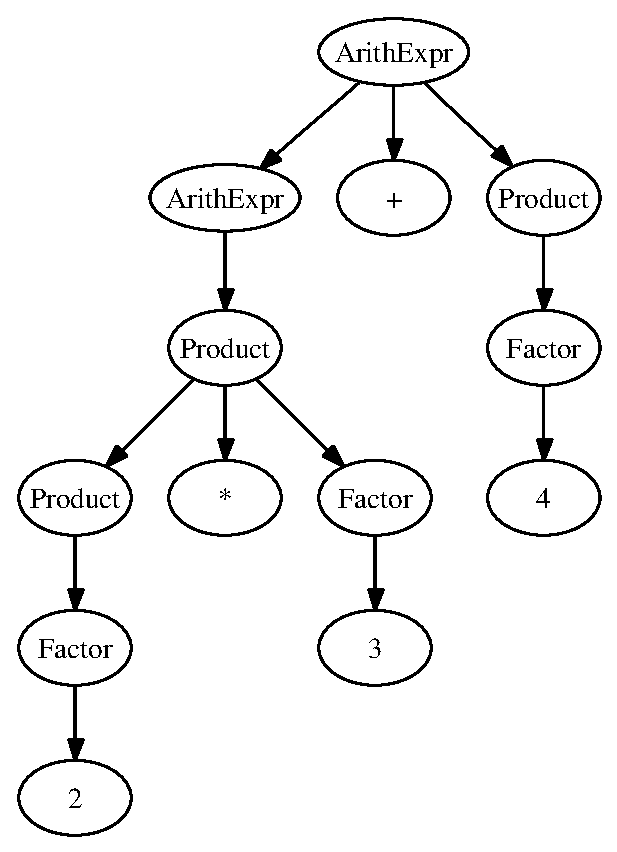
\epsfig{file=Abbildungen/parse-tree.eps, scale=0.6}
  \caption{Ein Parse-Baum f�r den String ``\texttt{2*3+4}''.}
  \label{fig:parse-tree.dot2}
\end{figure}

Fassen wir diesen Parse-Baum als Liste seiner
Zweige auf, wobei jeder Zweig eine Liste von Grammatik-Symbolen ist, so erhalten wir die folgende Liste:
\\[0.2cm]
\hspace*{1.3cm}
$
\begin{array}[b]{rl}
  \bigl[ 
 & [ \textsl{ArithExpr}, \textsl{ArithExpr}, \textsl{Product}, \textsl{Product}, \textsl{Factor}, \quoted{2} ],
   \\[0.1cm] 
 & [ \textsl{ArithExpr}, \textsl{ArithExpr}, \textsl{Product}, \quoted{*} ],
   \\[0.1cm] 
 & [ \textsl{ArithExpr}, \textsl{ArithExpr}, \textsl{Product}, \textsl{Factor}, \quoted{3} ],
   \\[0.1cm] 
 & [ \textsl{ArithExpr}, \quoted{+} ],
   \\[0.1cm] 
 & [ \textsl{ArithExpr}, \textsl{Product}, \textsl{Factor}, \quoted{4} ]
   \\[0.1cm] 
  \bigr]. 
\end{array}
$ \eox
\pagebreak

\noindent
Die nun folgende Definition der Funktion $\textsl{parseTree}()$ formalisiert die
Berechnung des Parse-Baums.

\begin{Definition}[\textsl{parseTree}] \lb
Ist $G = \langle V, T, R, S \rangle$ eine kontextfreie Grammatik, ist $w \in T^*$, $A \in V$ und  gibt es eine Ableitung
\[ A \Rightarrow^* w,  \]
so definieren wir $\textsl{parseTree}(A \Rightarrow^* w)$ induktiv als Liste von Listen:
\begin{enumerate}
\item Falls $(A \rightarrow t_1t_2 \cdots t_m)\in R$ mit $A \in V$ und $t_1 \cdots t_n = w$ ist,
      so setzen wir
      \[ \textsl{parseTree}(A \Rightarrow^*t) = \bigl[\, [A, t_1],\,  [A, t_2],\,\cdots,\,  [A, t_m]\, \bigr].  \]
\item Falls  $A \Rightarrow^* w$ gilt, weil
      \[ (A \rightarrow B_1B_2 \cdots B_m) \in R, \quad 
         B_i \Rightarrow^* w_i\; \mbox{f�r alle $i=1,\cdots,m$} \quad
         \mbox{und} \; w = w_1w_2 \cdots w_m
      \]
      gilt, so definieren wir (unter Benutzung der \textsc{SetlX}-Notation f�r die Definition von Listen)
      \[ 
        \textsl{parseTree}(A \Rightarrow^*w)  =
        \bigl[\; [A] + l \,:\,
                 i \in [1, \cdots, m ],\, l \in \textsl{parseTree}(B_i \Rightarrow^* w_i) \;
        \bigr]. 
      \]

      Damit diese Definition auch tats�chlich alle F�lle abdeckt, m�sen wir noch den Fall
      diskutieren, dass  eines der Symbole $B_i$ ein Terminal ist: In diesem Fall setzen wir
      \\[0.2cm]
      \hspace*{1.3cm}
      $\textsl{parseTree}(B_i \Rightarrow^* B_i) := \bigl[ [B_i] \bigr]$.
\end{enumerate}
\end{Definition}

Wir definieren die \emph{Breite} $b$ einer Grammatik als die gr��te Anzahl von Symbolen, die 
auf der rechten Seite einer Grammatik-Regel der Form
\\[0.2cm]
\hspace*{1.3cm}
$A \rightarrow \alpha$
\\[0.2cm]
auftreten.  

\begin{Lemma}[Beschr�nktheits-Lemma] \label{lemma:length}
  Die Grammatik $G = \langle V, T, R, S \rangle$ habe die Breite $b$.  Ferner gelte
  \\[0.2cm]
  \hspace*{1.3cm}
  $A \Rightarrow^* w$
  \\[0.2cm]
  f�r eine syntaktische Variable $A \in V$ und ein Wort $w \in T^*$.  Falls $n$ die L�nge der l�ngsten Liste in
  \[ \textsl{parseTree}(A \Rightarrow^* w) \]
  ist, so gilt f�r die L�nge des Wortes $w$ die Absch�tzung
  \\[0.2cm]
  \hspace*{1.3cm}
  $|w| \leq b^{n-1}$.  
\end{Lemma}

\noindent
\textbf{Beweis}: Wir f�hren den Beweis durch Induktion nach der L�nge $n$ der l�ngsten
Liste in $\textsl{parseTree}(A \Rightarrow^* w)$.
\begin{enumerate}
\item[I.A.] $n=2$:  Wenn alle Listen in $\textsl{parseTree}(A \Rightarrow^* w)$ 
            nur zwei Elemente haben, dann besteht die Ableitung aus genau einem Schritt
            und daher muss es eine Regel der Form 
            \\[0.2cm]
            \hspace*{1.3cm}
            $A \rightarrow t_1t_2 \cdots t_m$ \quad mit $w = t_1t_2 \cdots t_m$ und $t_i \in T$
            f�r alle $i=1,\cdots,m$
            \\[0.2cm]
            in der Grammatik $G$ geben.  Es gilt dann
            \[ \textsl{parseTree}(A \Rightarrow^* w) = 
               \bigl[\, [A,t_1],\, [A,t_2],\, \cdots,\; [A,t_m]\, \bigr].\, 
            \]
            Daraus folgt
            \\[0.2cm]
            \hspace*{1.3cm}
            $|w| = |t_1t_2 \cdots t_m| = m \leq b = b^{1} = b^{2-1}$,
            \\[0.2cm]
            wobei die Ungleichung $m \leq b$ aus der Tatsache folgt, dass die L�nge der Regeln der Grammatik
            $G$ durch die Breite $b$ beschr�nkt ist.
\item[I.S.] $n \mapsto n+1$: Da die Ableitung nun aus mehr als einem Schritt besteht, hat die Ableitung die Form
            \\[0.2cm]
            \hspace*{1.3cm}
            $A \Rightarrow B_1 B_2 \cdots B_m \Rightarrow^* w_1 w_2 \cdots w_m = w$.
            \\[0.2cm]
            Au�erdem haben dann die Listen in
            \[ 
               \textsl{parseTree}(B_i \Rightarrow^* w_i) 
            \]
            f�r alle $i=1,\cdots,m$ h�chstens die L�nge $n$.
            Nach Induktions-Voraussetzung wissen wir also, dass
            \\[0.2cm]
            \hspace*{1.3cm}
            $|w_i| \leq b^{n-1}$ \quad f�r alle $i=1,\cdots,m$
            \\[0.2cm]
            gilt.  Daher haben wir
            \\[0.2cm]
            \hspace*{1.3cm}
            $|w| = |w_1| + \cdots + |w_m| \leq b^{n-1} + \cdots + b^{n-1} = 
             m \cdot b^{n-1} \leq b \cdot b^{n-1} = b^{n} = b^{(n+1)-1}
            $. \qed
\end{enumerate}

\section{Das Pumping-Lemma f�r kontextfreie Sprachen}
\begin{Satz}[Pumping-Lemma]
Es sei $L$ eine kontextfreie Sprache.  Dann gibt es ein $n \in \mathbb{N}$, so dass jeder String
$s \in L$, dessen L�nge gr��er oder gleich $n$ ist, in der Form 
\[ s = uvwxy \]
geschrieben werden kann, so dass au�erdem folgendes gilt:
\begin{enumerate}
\item $|vwx| \leq n$,

      der mittlere Teil des Strings hat folglich eine L�nge von h�chstens $n$ Buchstaben.
\item $vx \not= \varepsilon$,

      die Teilstrings $v$ und $x$ k�nnen also nicht beide gleichzeitig leer sein.
\item $\forall h \in \mathbb{N}: uv^hwx^hy \in L$.

      die Strings $v$ und $x$ k�nnen beliebig oft repliziert (\emph{gepumpt}) werden. 
\end{enumerate}
\end{Satz}

\noindent
\textbf{Beweis}:  Da $L$ eine kontextfreie Sprache ist, gibt es eine kontextfreie
Grammatik $G = \langle V, T, R, S \rangle$, so dass 
\[ L = L(G) \]
gilt. Wir nehmen an, dass die Grammatik $G$ insgesamt $k$ syntaktische Variablen enth�lt
und au�erdem die 
Breite $b$ hat.  Wir definieren
\\[0.2cm]
\hspace*{1.3cm}
$n := b^{k+1} + 1$. 
\\[0.2cm] 
Sei nun $s \in L$ mit $|s| \geq n$.  Wir w�hlen einen Parse-Baum $\tau$ aus, der einerseits
den String $s$ ableitet und der andererseits unter allen Parse-B�umen, die den String $s$
aus $S$ ableiten, die minimale Anzahl von Knoten hat.  F�r diesen Parse-Baum $\tau$
betrachten wir die Listen aus
\\[0.2cm]
\hspace*{1.3cm}
$\tau = \textsl{parseTree}(S \Rightarrow^* s)$. 
\\[0.2cm] 
Falls alle Listen hier eine L�nge kleiner-gleich $k+1$ h�tten, so w�rde aus den Beschr�nktheits-Lemma
\ref{lemma:length} folgen, dass  
\\[0.2cm]
\hspace*{1.3cm}
$ |s| \leq b^{(k+1)-1} = b^k < b^{k+1} + 1 = n, \quad \mbox{also} \quad |s| < n$
\\[0.2cm] 
gilt, im Widerspruch zu der Voraussetzung $|s| \geq n$.  Also muss es in 
$\tau$ eine Liste geben, die mindestens die L�nge $k + 2$
hat.  Wir w�hlen die l�ngste Liste unter den  Listen in $\tau$ aus.
Diese Liste hat dann die Form
\[ [A_1, \cdots, A_l, t] \quad \mbox{mit $A_i \in V$ f�r alle $i \in \{1,\cdots,l\}$},\quad t \in T,
   \quad \mbox{sowie $l \geq k+1$}.
 \]
Wegen $l \geq k + 1$  k�nnen nicht alle Variablen $A_1$, $\cdots$, $A_l$
voneinander verschieden sein, denn es gibt ja nur insgesamt $k$ verschiedene syntaktische
Variablen.   Wir finden daher in der Menge $\{ l, l-1, \cdots, l-k \}$
zwei verschiedene Indizes $i$ und $j$,  so dass die Variablen $A_i$ und $A_j$ gleich sind und definieren
$A := A_i = A_j$.  Von den beiden Indizes $i$ und $j$ bezeichne $i$ den kleineren Index,
es gelte also $i < j$.   Die Ableitung von $s$ aus $S$ hat dann die folgende Form
\[ S \Rightarrow^* u A_i y \Rightarrow^* u v A_j x y \Rightarrow^* u v w x y = s. \] 
Insbesondere gilt also
\[ S \Rightarrow^* u A y, \quad A \Rightarrow^* vAx, \quad \mbox{und} \quad A \Rightarrow^* w. \]
Damit haben wir aber folgendes:
\begin{enumerate}
\item $S \Rightarrow^* uAy \Rightarrow^* uwy$, also
      \[ S \Rightarrow^* uv^0wx^0y. \]
\item $S \Rightarrow^* uAy \Rightarrow^* uvAxy \Rightarrow^* uvvAxxy \Rightarrow^* uvvwxxy$, also
      \[ S \Rightarrow^* uv^2wx^2y. \]
\item $S \Rightarrow^* uAy \Rightarrow^* uvAxy \Rightarrow^* uv^2Ax^2y \Rightarrow^* uv^3Ax^3y
       \Rightarrow^* \cdots \Rightarrow^* uv^hAx^hy \Rightarrow^* uv^hwx^hy$, also
      \\[0.2cm]
      \hspace*{1.3cm}
      $uv^hwx^hy \in L$ \quad f�r beliebige $h \in \mathbb{N}$.
      \vspace*{0.2cm}

\end{enumerate}
Wir m�ssen jetzt noch zeigen, dass $vx \not= \varepsilon$ gilt.  Die Ableitung
\[ A \Rightarrow^* vAx \]
ist eigentlich die Ableitung
\[ A_i \Rightarrow^* vA_jx \]
und enth�lt daher mindestens einen Ableitungsschritt.
Wir f�hren den Nachweis der Behauptung $vx \not= \varepsilon$ indirekt und nehmen $v = x =
\varepsilon$ an.
Dann w�rde wegen $A_i = A_j$ also
\\[0.2cm]
\hspace*{1.3cm}
$A_i \Rightarrow^+ A_i$
\\[0.2cm]
gelten, wobei das Zeichen $^+$ an dem Pfeil $\Rightarrow$ anzeigt, dass diese Ableitung
mindestens einen Schritt 
enth�lt.  In diesem Fall w�re aber der Parse-Baum $\tau$ nicht minimal, denn wir k�nnten
die Ableitungs-Schritte, die $A_i$ in $A_i$ �berf�hren, einfach weglassen.
Damit ist die Annahme $vx = \varepsilon$ widerlegt und es muss $vx \not= \varepsilon$ gelten.
\vspace*{0.2cm}

Als letztes zeigen wir, dass die Ungleichung $|vwx| \leq n$ gilt.  Wir haben
\[ A = A_i \Rightarrow^* vA_jx \Rightarrow^* vwx. \]
Weil einerseits $i \in \{l-k, l-(k-1), \cdots,l \}$ gilt und andererseits die der
Ableitung
$A \Rightarrow^* vwx$ zugeordnete Liste aus $\textsl{parseTree}(S \Rightarrow^* w)$ von
maximaler L�nge war, wissen wir, 
dass die L�nge der l�ngsten Liste in 
\[ \textsl{parseTree}(A \Rightarrow^* vwx) \]
kleiner-gleich  $k+2$ ist.
  Nach dem Beschr�nktheits-Lemma
\ref{lemma:length} folgt damit f�r die L�nge von $vwx$ die Absch�tzung
\\[0.2cm]
\hspace*{1.3cm}
$|vwx| \leq b^{(k+2)-1} = b^{k+1} < b^{k+1} + 1 = n$.   \qed


\remark
Das Pumping-Lemma wird in der deutschsprachigen Literatur gelegentlich  als 
``\emph{Schleifensatz}'' bezeichnet. 

\section{Anwendungen des Pumping-Lemmas}
Wir zeigen, wie mit Hilfe des Pumping-Lemmas der Nachweis erbracht werden kann, dass
bestimmte Sprachen nicht kontextfrei sind.

\subsection{Die Sprache $L = \{ \mathtt{a}^k \mathtt{b}^k \mathtt{c}^k \mid k \in \mathbb{N} \}$ ist
nicht kontextfrei}
Wir weisen nun nach, dass die Sprache
\[ L = \{ \mathtt{a}^k \mathtt{b}^k \mathtt{c}^k \mid k \in \mathbb{N} \} \]
nicht kontextfrei ist.  Wir f�hren diesen Nachweis indirekt und nehmen zun�chst an, dass $L$
kontextfrei ist.  Nach dem Pumping-Lemma gibt es dann eine nat�rliche Zahl $n$, so dass jeder String
$s \in L$, dessen L�nge gr��er oder gleich $n$ ist, sich in Teilstrings der Form
\[ s = uvwxy \]
zerlegen l�sst, so dass au�erdem folgendes gilt:
\begin{enumerate}
\item $|vwx| \leq n$,
\item $vx \not= \varepsilon$,
\item $\forall i \in \mathbb{N}: uv^iwx^iy \in L$.

      Insbesondere k�nnen wir hier $i=0$ w�hlen und erhalten dann
      $uwy \in L$. 
\end{enumerate}
Wir definieren nun den String $s$ wie folgt:
\[ s := \mathtt{a}^n\mathtt{b}^n\mathtt{c}^n. \]
Dieser String hat die L�nge $3 \cdot n \geq n$ und erf�llt damit die Voraussetzung �ber die L�nge.
Damit finden wir also eine Zerlegung $s=uvwxy$ mit den obigen Eigenschaften.  Da der Teilstring
$vwx$ eine L�nge kleiner oder gleich $n$ hat, k�nnen in diesem String nicht gleichzeitig die
Buchstaben \qote{a} und \qote{c} vorkommen. Wir betrachten die nach dieser Erkenntnis noch
m�glichen  F�lle getrennt.
\begin{enumerate}
\item Fall: In dem String $vwx$ kommen nur die Buchstaben \qote{a} und \qote{b} vor,  der Buchstabe
      \qote{c} kommt nicht vor: 
      \\[0.2cm]
      \hspace*{1.3cm}
      $\textsl{count}(vwx,\mathtt{c}) = 0$.
      \\[0.2cm]
      Da $vx \not= \varepsilon$ ist, folgt
      \\[0.2cm]
      \hspace*{1.3cm}
      $\textsl{count}(vx,\mathtt{a}) + \textsl{count}(vx,\mathtt{b}) > 0$.
      \\[0.2cm]
      Wir nehmen zun�chst an, dass $\textsl{count}(vx,\mathtt{a}) > 0$ gilt,
      der Fall $\textsl{count}(vx,\mathtt{b}) > 0$ ist analog zu behandeln.
      Dann erhalten wir einerseits
      \[ 
      \begin{array}[t]{lcl}
        \textsl{count}(uwy,\mathtt{c}) & = & \textsl{count}(s,\mathtt{c}) - \textsl{count}(vx,\mathtt{c}) \\
                              & = & \textsl{count}(s,\mathtt{c}) - 0 \\
                              & = & \textsl{count}(\mathtt{a}^n\mathtt{b}^n\mathtt{c}^n,\mathtt{c}) \\
                              & = & n.
      \end{array}
      \]
      Z�hlen wir nun die H�ufigkeit, mit welcher der Buchstabe \qote{a}
      in dem String $uwy$ auftritt, so erhalten wir
      \[ 
      \begin{array}[t]{lcl}
        \textsl{count}(uwy,\mathtt{a}) & = & 
        \textsl{count}(s,\mathtt{a})  - \textsl{count}(vx,\mathtt{a}) \\
                              & < & \textsl{count}(s,\mathtt{a}) \\
                              & = & \textsl{count}(\mathtt{a}^n\mathtt{b}^n\mathtt{c}^n,\mathtt{a}) \\
                              & = & n.
      \end{array}
      \]
      Damit haben wir dann aber
      \\[0.2cm]
      \hspace*{1.3cm}
      $\textsl{count}(uwy,\mathtt{a}) < \textsl{count}(uwy,\mathtt{c})$
      \\[0.2cm]
      und daraus folgt $uwy \not\in L$, was im Widerspruch zum Pumping-Lemma steht.
\item Fall: In dem String $vwx$ kommt der Buchstabe \qote{a} nicht vor.
   
      Dieser Fall l�sst sich analog zum ersten Fall behandeln. \qed
\end{enumerate}

\exercise
Zeigen Sie, dass die Sprache 
\[ L = \bigl\{ \,\mathtt{a}^{k^2} \;\big|\; k \in \mathbb{N}\, \bigr\} \]
nicht kontextfrei ist.
\vspace*{0.2cm}

\noindent
\textbf{Hinweis}: Argumentieren Sie �ber die L�nge der betrachteten Strings.
\vspace*{0.2cm}

\solution
Wir f�hren den Beweis indirekt und nehmen an, dass die Sprache $L_{\mathrm{square}}$ kontextfrei
w�re.  Nach dem Pumping-Lemma f�r kontextfreie Sprachen gibt es dann eine positive
nat�rliche Zahl $n$, so dass sich jeder String $s \in L_{\mathrm{square}}$ mit $|s| \geq n$ in f�nf 
Teilstrings $u$, $v$, $w$, $x$, und $y$ aufspalten l�sst, so dass gilt:
\begin{enumerate}
\item $s = uvwxy$,
\item $|vwx| \leq n$,
\item $vx \not= \varepsilon$,
\item $\forall h \in \mathbb{N}: uv^hwx^hy \in L_{\mathrm{square}}$. 
\end{enumerate} 
Wir betrachten nun den String $s = a^{n^2}$.  F�r die L�nge dieses Strings gilt offenbar
\[ |s| = \big| a^{n^2} \big| = n^2 \geq n. \]
Also gibt es eine Aufspaltung von $s$ der Form $s = uvwxy$ mit den oben angegebenen Eigenschaften.
Da $a$ der einzige Buchstabe ist, der in $s$ vorkommt, k�nnen in den Teilstrings $u$, $v$, $w$, $x$ und $y$
auch keine anderen Buchstaben vorkommen und es muss nat�rliche Zahlen $c$, $d$, $e$, $f$, und $g$ geben, so
dass  
\[ u = a^c,\; v = a^d,\; w = a^e,\; x = a^f\; \mbox{und}\; y = a^g \]
gilt.  Wir untersuchen, welche Konzequenzen sich daraus f�r die Zahlen $c$, $d$, $e$, $f$, $g$ ergeben.
\begin{enumerate}
\item Die Zerlegung $s = uvwxy$ schreibt sich als $a^{n^2} = a^ca^da^ea^fa^g$ und daraus folgt
      \begin{equation}
        \label{eq:e1}
         n^2 = c + d + e + f + g.     
      \end{equation}
\item Aus der Ungleichung $|vwx| \leq n$ folgt  
      \begin{equation}
        \label{eq:e2}
        d + e + f \leq n.
      \end{equation}
\item Die Bedingung $vx \not= \varepsilon$ liefert
      \begin{equation}
        \label{eq:e3}
        d + f > 0.
      \end{equation}
\item Aus der Formel $\forall h \in \mathbb{N}: uv^hwx^hy \in L_{\mathrm{square}}$ folgt
      \begin{equation}
        \label{eq:e4}
        \forall h \in \mathbb{N}: a^ca^{d\cdot h}a^ea^{f\cdot h}a^g \in L_{\mathrm{square}}. 
      \end{equation}
\end{enumerate}
Die letzte Gleichung muss insbesondere auch f�r den Wert $h=2$ gelten:
\[ a^ca^{2\cdot d}a^ea^{2\cdot f}a^g \in L_{\mathrm{square}}.  \]
Nach Definition der Sprache $L_{\mathrm{square}}$ gibt es dann eine nat�rliche Zahl
$k$, so dass gilt
\begin{equation}
  \label{eq:e5}
  c + 2\cdot d + e + 2\cdot f + g = k^2.
\end{equation}
Addieren wir in Gleichung (\ref{eq:e1}) auf beiden Seiten $d+f$, so erhalten wir insgesamt
\[ n^2 + d + f = c + 2\cdot d + e + 2\cdot f + g = k^2. \]
Wegen $d + f > 0$ folgt daraus 
\begin{equation}
  \label{eq:e6}
  n < k.    
\end{equation}
Andererseits haben wir
\[ 
\begin{array}[t]{lcll}
 k^2  & =    & c + 2\cdot d + e + 2\cdot f + g   & \mbox{nach Gleichung (\ref{eq:e5}})   \\
      & =    & (c + d + e + f + g) + (d + f)     & \mbox{elementare Umformung}           \\
      & \leq & (c + d + e + f + g) + (d + e + f) & \mbox{denn $e \geq 0$}                \\
      & \leq & (c + d + e + f + g) + n           & \mbox{nach Ungleichung (\ref{eq:e2}}) \\
      & =    & n^2 + n                           & \mbox{nach Gleichung (\ref{eq:e1}})   \\
      & <    & n^2 + 2 \cdot n + 1               & \mbox{da $n+1 > 0$}                   \\ 
      & =    & (n+1)^2                           & \mbox{elementare Umformung}           \\ 
\end{array}
\]
Damit haben wir insgesamt  $k^2 < (n+1)^2$ gezeigt und das impliziert
\begin{equation}
  \label{eq:e7}
  k < n+1.
\end{equation}
Zusammen mit Ungleichung (\ref{eq:e6}) liefert Ungleichung (\ref{eq:e7}) nun die Ungleichungs-Kette
\[ n < k < n + 1. \]
Da andererseits $k$ eine nat�rliche Zahl sein muss und $n$ ebenfalls eine nat�rliche Zahl ist,
haben wir jetzt einen Widerspruch, denn zwischen $n$ und $n+1$ gibt es keine nat�rliche Zahl.
\qed


\exercise
Das Alphabet $\Sigma$ sei durch die Festlegung $\Sigma := \{ \mathtt{a}, \mathtt{b} \}$
definiert.  Zeigen Sie, dass die Sprache 
\[ L = \bigl\{ \, tt \;\big|\; t \in \Sigma^*\, \bigr\} \]
nicht kontextfrei ist.

\solution
Wir f�hren den Beweis indirekt und nehmen an, dass die Sprache $L$ kontextfrei
w�re.  Nach dem Pumping-Lemma f�r kontextfreie Sprachen gibt es dann eine positive
nat�rliche Zahl $n$, so dass sich jeder String $s \in L$ mit $|s| \geq n$ in f�nf 
Teilstrings $u$, $v$, $w$, $x$, und $y$ aufspalten l�sst, so dass gilt:
\begin{enumerate}
\item $s = uvwxy$,
\item $|vwx| \leq n$,
\item $vx \not= \varepsilon$,
\item $\forall h \in \mathbb{N}: uv^hwx^hy \in L$. 
\end{enumerate} 
Wir betrachten nun den String $s := a^{n}b^{n}a^{n}b^{n}$.  Definieren wir $t:= a^nb^n$,
so ist klar, dass $s = tt$ ist und damit gilt $s \in L$.
F�r die L�nge von $s$ gilt 
\[ |s| = \big| a^{n}b^{n}a^{n}b^{n} \big| = 4 \cdot n \geq n. \]
Also gibt es nach dem Pumping-Lemma eine Aufspaltung von $s$ der Form $s = uvwxy$ mit den
oben angegebenen Eigenschaften. 
Im weiteren f�hren wir eine Fallunterscheidung nach der Lage des Strings $vwx$ innerhalb
des gesamten Strings $s = a^{n}b^{n}a^{n}b^{n}$ durch.  Dabei ber�cksichtigen wir, dass
$|vwx| \leq n$ gilt.  Zur Vereinfachung der Darstellung des Beweises vereinbaren wir f�r zwei Strings
$r$ und $s$ die Schreibweise 
\\[0.2cm]
\hspace*{1.3cm}
$r \sqsubseteq s$ \quad g.d.w. \quad $r$ ist Teilstring von $s$.
\\[0.2cm]
Wollen wir zus�tzlich die Position einschr�nken, an der $r$ innerhalb von $s$ auftritt, so
schreiben wir
\\[0.2cm]
\hspace*{1.3cm}
$r \sqsubseteq_{i,j} s$ \quad g.d.w. \quad
$r \sqsubseteq s[i \mathtt{..} j]$. 
\\[0.2cm]
Die Schreibweise $r \sqsubseteq_{i,j} s$ dr�ckt also aus, dass der Teilstring $r$ ab der
Position $i$ in dem String $s$ auftritt und dass das Ende $r$ nicht �ber die Position $j$ hinausreicht.


F�r die Lage des Teilstrings $vwx$ innerhalb von $a^{n}b^{n}a^{n}b^{n}$ gibt es aufgrund
der L�ngenbeschr�nkung $|vwx| \leq n$ nur drei M�glichkeiten:
\begin{enumerate}
\item Fall: \quad $vwx \sqsubseteq_{1,2\cdot n} a^{n}b^{n}a^{n}b^{n}$,  

      der Teilstring
      $vwx$ liegt also in der ersten H�lfte von $s$ und ist folglich Teil von
      $a^{n}b^{n}$.
\item Fall: \quad $vwx \sqsubseteq_{n+1,3\cdot n} a^{n}b^{n}a^{n}b^{n}$,  

      der Teilstring
      $vwx$ liegt in der Mitte von $s$ und ist Teil von $b^{n}a^{n}$.
\item Fall: \quad $vwx \sqsubseteq_{2\cdot n+1, 4 \cdot n} a^{n}b^{n}a^{n}b^{n}$,  
  
      der Teilstring
      $vwx$ liegt in der zweiten H�lfte von $s$ und ist folglich Teil von
      $a^{n}b^{n}$.
\end{enumerate}
Wir setzen nun im Pumping-Lemma in der vierten Aussage f�r $h$ den Wert $0$ ein und folgern, dass der
String 
\\[0.2cm]
\hspace*{1.3cm}
$uv^0wx^0y = uwy$ 
\\[0.2cm]
in der Sprache $L$ liegt.  Wir zeigen, dass dies zu einem Widerspruch
f�hrt und untersuchen dazu die obigen drei F�lle der Reihe nach.
\begin{enumerate}
\item Fall: \quad $vwx \sqsubseteq_{1,2\cdot n} a^{n}b^{n}a^{n}b^{n}$.

      Da $vx$ in der ersten H�lfte von
      $s = a^{n}b^{n}a^{n}b^{n}$ liegt und der String $uwy$ aus $s$ dadurch entsteht, dass
      wir $v$ und $x$ weglassen, hat der String $uwy$ die Form
      \\[0.2cm]
      \hspace*{1.3cm}
      $uwy = a^{n-k_1}b^{n-k_2}a^{n}b^{n}$
      \\[0.2cm]
      und wegen $vx \not= \varepsilon$ wissen wir, dass $k_1 + k_2 > 0$ ist.
      Die Mitte des Strings $uwy$ liegt daher innerhalb des Teilstrings $a^nb^n$.
      Wenn wir also 
      \\[0.2cm]
      \hspace*{1.3cm}
      $t't' = a^{n-k_1}b^{n-k_2}a^{n}b^{n}$ \quad f�r ein $t' \in \Sigma^*$
      \\[0.2cm]
      h�tten, so w�rde das erste Auftreten von $t'$ in den Teilstring $a^{n}$ hineinragen und m�sste folglich
      mit einem $a$ enden.  Das funktioniert aber nicht, denn
      das zweite Auftreten von $t'$ endet mit einem $b$.  Also kann dieser Fall nicht eintreten.
\item Fall: \quad $vwx \sqsubseteq_{n+1,3\cdot n} a^{n}b^{n}a^{n}b^{n}$,  

      Da $vx$ nun innerhalb von $s = b^{n}a^{n}$ liegt und der String $uwy$ aus $s$ dadurch
      entsteht, dass wir $v$ und $x$ weglassen, hat der String $uwy$ die Form
      \\[0.2cm]
      \hspace*{1.3cm} $uwy = a^{n}b^{n-k_1}a^{n-k_2}b^{n}$
      \\[0.2cm]
      Wenn $uwy \in L$ ist, m�sste es also ein $t'$ geben mit
      \\[0.2cm]
      \hspace*{1.3cm} $t't' = a^{n}b^{n-k_1}a^{n-k_2}b^{n}$ \quad und $t' \in \Sigma^*$.
      \\[0.2cm]
      Wenn wir uns das erste Auftreten von $t'$ in dieser Gleichung ansehen, stellen wir fest, dass $t'$ mit
      dem String $a^{n}$ beginnt.  Betrachten wir das zweite Auftreten von $t'$      , so sehen wir, dass 
      $t'$ mit dem String $b^{n}$ endet.  Damit hat dann aber $t'$ mindestens die L�nge $2
  \cdot n$ und $t't' = uwy$ 
      h�tte mindestens die L�nge $4 \cdot n$.  Wegen $vx \not= \varepsilon$  ist dies
      nicht m�glich und auch dieser Fall kann nicht eintreten.  

\item Fall: \quad $vwx \sqsubseteq_{2\cdot n+1, 4 \cdot n} a^{n}b^{n}a^{n}b^{n}$.
  
      Dieser Fall ist analog zum ersten Fall.
\end{enumerate}
Da wir in jedem Fall einen Widerspruch erhalten haben, k�nnen wir schlie�en, dass die Sprache $L$
nicht kontextfrei sein kann.
\qed
\pagebreak

\exercise
Zeigen Sie, dass die Sprache 
\[ L = \bigl\{ \,\mathtt{a}^{p} \;\big|\; \mbox{$p$ ist Primzahl}\, \bigr\} \]
nicht kontextfrei ist.

\solution
Wir f�hren den Beweis indirekt und nehmen an, $L$ w�re kontextfrei.  Nach
dem Pumping-Lemma gibt es dann eine Zahl $n$, so dass es f�r alle Strings $s \in L$, 
deren L�nge gr��er als $n$ ist, eine Zerlegung
\\[0.2cm]
\hspace*{1.3cm}
$s = uvwxy$
\\[0.2cm]
mit den folgenden drei Eigenschaften gibt:
\begin{enumerate}
\item $|vwx| \leq n$ \quad und
\item $vx \not= \varepsilon$, 
\item $\forall h \in \mathbb{N}: u v^h w x^h y \in L$.
\end{enumerate}
Wir w�hlen nun eine Primzahl $p$, die gr��er als $n+1$ ist und setzen $s = \mathtt{a}^p$.
Dann gilt $|s| = p > n$ und die Voraussetzung des Pumping-Lemmas ist erf�llt.
Wir finden also eine Zerlegung von $\mathtt{a}^p$ der Form
\\[0.2cm]
\hspace*{1.3cm}
$\mathtt{a}^p = uvwxy$ 
\\[0.2cm]
mit den oben angegebenen Eigenschaften.
Aufgrund der Gleichung $s = uvwxy$ k�nnen die Teilstrings $u$, $v$, $w$, $x$ und $y$ nur aus dem
Buchstaben ``\texttt{a}'' bestehen.  Also gibt es nat�rliche Zahlen $c$, $d$, $e$, $f$ und
$g$ so dass gilt:
\\[0.2cm]
\hspace*{1.3cm}
$u = \mathtt{a}^c$, \quad $v = \mathtt{a}^d$, \quad $w = \mathtt{a}^e$, \quad 
$x = \mathtt{a}^f$ \quad und \quad $y = \mathtt{a}^g$.
\\[0.2cm]
F�r die Zahlen $c$, $d$, $e$, $f$ und $g$ gilt dann Folgendes:
\begin{enumerate}
\item $c + d + e + f + g = p$,
\item $d + f \not= 0$,
\item $d + e + f \leq n$,
\item $\forall h \in \mathbb{N}: c + h \cdot d + e + h \cdot f + g \in \mathbb{P}$.
\end{enumerate}
Setzen wir in der letzten Gleichung f�r $h$ den Wert $(c + e + g)$ ein, so erhalten wir
\\[0.2cm]
\hspace*{1.3cm}
$c + (c + e + g) \cdot d + e + (c + e + g) \cdot f + g \in P$.
\\[0.2cm]
Wegen
\\[0.2cm]
\hspace*{1.3cm}
$c + (c + e + g) \cdot d + e + (c + e + g) \cdot f + g = (c + e + g) \cdot (1 + d + f)$ 
\\[0.2cm]
h�tten wir dann
\\[0.2cm]
\hspace*{1.3cm}
$(c + e + g) \cdot (1 + d + f) \in \mathbb{P}$.
\\[0.2cm]
Dass kann aber nicht sein, denn wegen $d + f > 0$ ist der Faktor $1 + d + f$ von 1
verschieden und wegen $d + e + f \leq n$ und $c + d + e + f + g = p$ und $p > n + 1$ wissen
wir, dass 
$c + g > 1$ ist, so dass auch der Faktor $(c + e + g)$ von 1 verschieden ist.  Damit kann das
Produkt $(c + e + g) \cdot (1 + d + f)$ aber keine Primzahl mehr sein und wir haben einen
Widerspruch zu der Annahme, dass $L$ kontextfrei ist.
\qed

%%% Local Variables: 
%%% mode: latex
%%% TeX-master: "formal-languages"
%%% End: 

%\chapter{Keller-Automaten}
In diesem Kapitel stellen wir die \emph{Keller-Automaten} (engl.~\emph{push-down automata})
vor.  Wir werden sehen, dass dieses Automaten-Modell zu dem Konzept der kontextfreien Sprachen
�quivalent ist:  Eine Sprache $L$ ist genau dann kontextfrei, wenn es einen
nicht-deterministischen Keller-Automaten gibt, der die Sprache $L$ erkennt.  Insofern verhalten
sich Keller-Automaten zu den kontextfreien Sprachen genauso, wie sich die endlichen Automaten
zu den regul�ren Sprachen verhalten.  Im Vergleich zur Theorie der endlichen Automaten hat die
Theorie der Keller-Automaten allerdings einen Sch�nheitsfehler:  W�hrend die deterministischen
endlichen Automaten zu den nicht-deterministischen endlichen Automaten �quivalent sind, sind
die nicht-deterministischen Keller-Automaten m�chtiger als die deterministischen
Keller-Automaten, denn es gibt kontextfreie Sprachen, die sich zwar mit einem
nicht-deterministischen Keller-Automaten erkennen lassen, f�r die es aber keinen
deterministischen Keller-Automaten gibt, der diese Sprache erkennt.  Allerdings werden wir
sehen, dass die meisten f�r die Praxis interessanten kontextfreien Sprachen bereits von
deterministischen Keller-Automaten erkannt werden.
    
\section{Definition eines Keller-Automaten}
Im Allgemeinen werden Keller-Automaten als endliche Automaten definiert, die zus�tzlich mit
einem Kellerspeicher (engl.~\emph{stack}) ausgestattet sind, auf dem Werte abgelegt werden k�nnen.  Der
Zustand eines Automaten setzt sich dann aus zwei Komponenten zusammen:
\begin{enumerate}
\item Dem Inhalt des Kellerspeichers und
\item dem Zustand des zugrunde liegenden endlichen Automaten.
\end{enumerate}
Es zeigt sich aber, dass der Kellerspeicher als Ged�chtnis bereits ausreichend ist, eine weitere
Komponente wird nicht ben�tigt.  Wir werden uns in unseren Betrachtungen zun�chst auf diese Art von
Keller-Automaten beschr�nken.

\begin{Definition}[Keller-Automat]
  Ein \emph{Keller-Automat} $A$ ist ein 4-Tupel
  \\[0.2cm]
  \hspace*{1.3cm}
  $A = \langle \Sigma, \Gamma, \delta, S_0 \rangle$,
  \\[0.2cm]
  wobei die Komponenten die folgende Bedeutung haben:
  \begin{enumerate}
  \item $\Sigma$ ist das \emph{Eingabe-Alphabet}, der Keller-Automat verarbeitet also W�rter aus
        $\Sigma^*$.
  \item $\Gamma$ ist das \emph{Keller-Alphabet}.

        In der Praxis ist $\Gamma$ h�ufig eine Obermenge von $\Sigma$.
  \item $\delta$ ist die \emph{�bergangs-Funktion}.  
        Als Argument bekommt diese Funktion entweder einen Buchstaben
        aus dem Eingabe-Alphabet $\Sigma$ und einen Buchstaben aus dem Keller-Alphabet
        $\Gamma$, oder das Zeichen $\varepsilon$ und einen Buchstaben aus $\Gamma$.
        Als Ausgabe liefert diese Funktion eine Menge von Strings aus dem Keller-Alphabet,
        es gilt also
        \\[0.2cm]
        \hspace*{1.3cm}
        $\delta: (\Sigma \cup \{ \varepsilon \}) \times \Gamma \rightarrow \textsl{Pow}\bigl(\Gamma^*\bigr)$.
        \\[0.2cm]
        Hier bezeichnet $\textsl{Pow}(\Gamma^*)$ die Potenz-Menge von $\Gamma^*$, also die
        Menge aller Teilmengen von $\Gamma^*$ und $\Gamma^*$ bezeichnet die Menge der
        W�rter �ber $\Gamma$.
  \item $S_0$ ist das Start-Symbol, das ein Element des Keller-Alphabets $\Gamma$ ist:
        \\[0.2cm]
        \hspace*{1.3cm}
        $S_0 \in \Gamma$.
        \\[0.2cm]
        Zu Beginn der Rechnung eines Keller-Automaten liegt im Kellerspeicher des
        Keller-Automaten genau dieses Start-Symbol und sonst nichts.  \qed
  \end{enumerate}
\end{Definition}

Wie funktioniert nun ein Keller-Automat?  Ein Wort $w \in \Sigma^*$ wird von dem
Keller-Automaten wie folgt verarbeitet. 
\begin{enumerate}
\item Zun�chst wird in dem leeren Kellerspeicher das Start-Symbol $S_0$ abgelegt.
\item Anschlie�end wird das Wort Buchstabe f�r Buchstabe gelesen, wobei sich der 
      Kellerspeicher des Automaten wie folgt ver�ndern kann:
      \begin{enumerate}
      \item Ist $C$ der Buchstabe, der im Kellerspeicher (also auf dem Stack) ganz oben liegt, 
            und gilt $\alpha \in \delta(\varepsilon, C)$, dann wird der Buchstabe $C$ 
            aus dem Kellerspeicher entfernt und die Buchstaben aus $\alpha$ werden so eingekellert
            dass der erste Buchstabe aus $\alpha$  oben auf dem Stack liegt.
            Da $\alpha$ auch das leere Wort sein kann, kann der Stack dabei auch schrumpfen.

            In diesem Fall wird kein Buchstabe des Wortes $w$ gelesen.
      \item Ist $C$ der Buchstabe, der im Kellerspeicher (also auf dem Stack) ganz oben liegt, ist
            $b$ der n�chste zu lesende Buchstabe aus dem Wort $w$ und gilt
            $\alpha \in \delta(b, C)$, dann wird der Buchstabe $b$ gelesen, der Buchstabe
            $C$ wird aus dem Kellerspeicher entfernt und anschlie�end werden die Buchstaben aus
            $\alpha$ eingekellert. 
      \end{enumerate}
      Keller-Automaten sind nicht-deterministisch, denn beispielsweise kann f�r       
      $\alpha_1 \not= \alpha_2$ sowohl 
      \\[0.2cm]
      \hspace*{1.3cm}
      $\alpha_1 \in \delta(b,C)$, \quad als auch \quad $\alpha_2 \in \delta(b,C)$ gelten,
      \\[0.2cm]
      und dann hat der Automat die Wahl, ob er $\alpha_1$ oder $\alpha_2$ einkellert.
      Genauso kann es sein, dass gleichzeitig
      \\[0.2cm]
      \hspace*{1.3cm}
      $\alpha_1 \in \delta(\varepsilon,C)$ \quad und \quad $\alpha_2 \in \delta(b,C)$
      \\[0.2cm]
      gilt.  In diesem Fall hat der Automat die M�glichkeit, entweder das Zeichen
      $C$ im Kellerspeicher durch das Wort $\alpha_1$ zu ersetzen, ohne dabei einen Buchstaben zu lesen, oder
      der Automat kann den Buchstaben $b$ lesen und das Zeichen $C$ durch das Wort $\alpha_2$
      ersetzen.
\item Sind alle Buchstaben des Wortes $w$ gelesen, und ist gleichzeitig der Kellerspeicher geleert worden,
      dann akzeptiert der Keller-Automat das Wort $w$.
\end{enumerate}
Formal definieren wir die \emph{Konfiguration} eines Keller-Automaten $A = \langle \Sigma, \Gamma, \delta, S_0 \rangle$,
als ein Paar
\\[0.2cm]
\hspace*{1.3cm}
$\langle v, \alpha \rangle \in \Sigma^* \times \Gamma^*$,
\\[0.2cm]
dass aus einem Wort $v$ des Eingabe-Alphabets und einem weiteren Wort
$\alpha$  des Keller-Alphabets besteht.  Die Idee ist, dass $v$ den Teil des Eingabewortes
darstellt, der noch nicht gelesen wurde, w�hrend $\alpha$ den Zustand des Kellerspeicher  beschreibt. 
Wir definieren nun f�r zwei Konfigurationen $\pair(u,\alpha)$ und $\pair(v,\beta)$ des
Keller-Automaten $A$ eine
Relation 
\\[0.2cm]
\hspace*{1.3cm}
$\pair(u,\alpha) \vdash_A \pair(v,\beta)$
\\[0.2cm]
durch die folgenden beiden Klauseln:
\begin{enumerate}
\item $\alpha \in \delta(\varepsilon, C) \;\rightarrow\; \pair(w, C\beta) \vdash_A \pair(w,\alpha \beta)$.

      Hier hat der Keller-Automat $A$ einen $\varepsilon$-�bergang,
      bei dem das Stack-Symbol $C$ durch den String $\alpha$ ersetzt wird.
      Das Wort $w$ bleibt in diesem Fall unver�ndert.
      
\item $\alpha \in \delta(b, C) \;\rightarrow\; \pair(bu, C\beta) \vdash_A \pair(u,\alpha \beta)$.

      In diesem Fall hat der Keller-Automat $A$ f�r den Buchstaben $b$ und das
      Stack-Symbol einen �bergang, bei dem $b$ gelesen und das Stack-Symbol $C$ durch
      den String $\alpha$ ersetzt wird. 
\end{enumerate}
Wir bezeichnen den transitiven und reflexiven Abschluss der Relation $\vdash_A$ mit
$\vdash_A^*$.  Bei Diskussionen, in denen klar ist, um welchen Keller-Automaten $A$ es
sich handelt, lassen wir den Index $A$ auch weg und schreiben einfach $\vdash^*$ an Stelle
von $\vdash_A^*$.  Damit sind wir nun in der Lage, die von einem Keller-Automaten 
\\[0.2cm]
\hspace*{1.3cm}
$A = \langle \Sigma, \Gamma, \delta, S_0 \rangle$
\\[0.2cm]
akzeptierte Sprache $L(A)$ zu definieren:
\\[0.2cm]
\hspace*{1.3cm}
$L(A) := \bigl\{ w \in \Sigma^* \mid \pair(w,S_0) \vdash_A^* \pair(\varepsilon, []) \bigr\}$,
\\[0.2cm]
wobei wir hier mit $[]$ den leeren Kellerspeicher bezeichnen.  Ein Wort $w$ wird also genau dann
von dem Keller-Automaten $A$ akzeptiert,  wenn der Keller-Automat beim Lesen dieses Wortes
seinen Kellerspeicher leeren kann.

\example
Wir definieren den Keller-Automat $A = \langle \Sigma, \Gamma, \delta, S \rangle$ wie
folgt:
\begin{enumerate}
\item $\Sigma := \{ \texttt{a}, \texttt{b} \}$.
\item $\Gamma := \{ \texttt{a}, \texttt{b}, S \}$.
\item $\delta(\varepsilon, \texttt{a}) := \{ \}$, \quad 
      $\delta(\varepsilon, \texttt{b}) := \{ \}$, \quad
      $\delta(\varepsilon, S) := \{ \texttt{a}S\texttt{a}, \texttt{b}S\texttt{b}, \texttt{a}, \texttt{b}, \varepsilon \}$,

      $\delta(\texttt{a}, \texttt{a}) := \{ \varepsilon \}$, \quad
      $\delta(\texttt{a}, \texttt{b}) := \{ \}$, \quad
      $\delta(\texttt{a}, S) := \{ \}$, 

      $\delta(\texttt{b}, \texttt{a}) := \{ \}$, \quad
      $\delta(\texttt{b}, \texttt{b}) := \{ \varepsilon \}$, \quad
      $\delta(\texttt{b}, S) := \{ \}$.

      Beachten Sie, dass es einen subtilen Unterschied zwischen den F�llen
      \\[0.2cm]
      \hspace*{1.3cm}
      $\delta(\texttt{a}, \texttt{a}) := \{ \varepsilon \}$ \quad und \quad
      $\delta(\texttt{a}, \texttt{b}) := \{ \}$
      \\[0.2cm]
      gibt:  Falls der n�chste Buchstaben des zu verarbeitenden Wortes ein ``\texttt{a}''
      ist und falls au�erdem ein ``\texttt{a}'' oben auf 
      dem Stack liegt, dann wird das ``\texttt{a}'' aus dem Wort gelesen und 
      das ``\texttt{a}'' auf dem Stack wird durch das leere Wort $\varepsilon$ ersetzt 
      und damit entfernt. 
      
      Ist hingegen  der n�chste Buchstaben des zu verarbeitenden Wortes ein ``\texttt{a}''
      und liegt  ein ``\texttt{b}'' oben auf dem Stack, so gibt es f�r den Automaten
      keinen �bergang und damit kann der Buchstabe ``\texttt{a}'' nicht gelesen werden.
      In diesem Fall sagen wir auch, dass der Automat \emph{stirbt}.
\item Das Start-Symbol ist $S$.
\end{enumerate}
Ist $w$ ein Wort, so bezeichnen wir mit $w^r$ das
Wort, das aus $w$ entsteht, wenn wir $w$ von hinten lesen.  Der erste Buchstabe von $w$
ist also der letzte Buchstabe von $w^r$, der zweite Buchstabe von $w$ ist der vorletzte
Buchstabe von $w^r$ und allgemein gilt f�r ein Wort der L�nge $n$
\\[0.2cm]
\hspace*{1.3cm}
$|w| = n \;\rightarrow\; \forall i \in \{1,\cdots,n\}:w^r[i] = w[n + 1 - i]$. 
\\[0.2cm]
Hier bezeichnet $|w|$ die L�nge des Wortes und $w[i]$ bezeichnet den $i$-ten Buchstaben.
W�rter, f�r die $w^r = w$ gilt, werden als \emph{Palindrome} bezeichnet.
Ein einfaches Beispiel ist das Wort 
\\[0.2cm]
\hspace*{1.3cm}
\texttt{aabaa}.
\\[0.2cm]
Wir behaupten, dass der oben definierte Automat $A$ genau die Palindrome erkennt, es gilt also
\\[0.2cm]
\hspace*{1.3cm}
$L(A) = \{ w \in \Sigma^* \mid w = w^r \}$
\\[0.2cm]
Wir zeigen, wie der Automat das Wort 
\\[0.2cm]
\hspace*{1.3cm}
\texttt{aabaa}
\\[0.2cm]
verarbeitet.
\begin{enumerate}
\item Der Automat startet mit der Konfiguration
      \\[0.2cm]
      \hspace*{1.3cm}
      $\pair(\texttt{aabaa},S)$ 
\item Da das oberste Symbol auf dem Stack ein $S$ ist, kann der Automat die Tatsache, dass
      \\[0.2cm]
      \hspace*{1.3cm}
      $\texttt{a}S\texttt{a} \in \delta(\varepsilon,S)$
      \\[0.2cm]
      ausnutzen und einen $\varepsilon$-�bergang durchf�hren.  Dabei wird dann die
      folgende Konfiguration erreicht:
      \\[0.2cm]
      \hspace*{1.3cm}
      $\pair(\texttt{aabaa},\texttt{a}S\texttt{a})$
\item Jetzt ist der erste Buchstabe des zu lesenden Wortes ein \texttt{a} und gleichzeitig
      liegt ein \texttt{a} auf dem Stack.  Also verwenden wir
      \\[0.2cm]
      \hspace*{1.3cm}
      $\varepsilon \in \delta(\texttt{a}, \texttt{a})$
      \\[0.2cm]
      und entfernen damit sowohl das erste ``\texttt{a}'' aus dem zu lesenden Wort als
      auch das ``\texttt{a}'' auf dem Stack und erhalten die Konfiguration
      \\[0.2cm]
      \hspace*{1.3cm}
      $\pair(\texttt{abaa}, S\texttt{a})$.
\item Wir benutzen wieder $\texttt{a}S\texttt{a} \in \delta(\varepsilon,S)$ und erhalten
      die Konfiguration
      \\[0.2cm]
      \hspace*{1.3cm}
      $\pair(\texttt{abaa}, \texttt{a}S\texttt{aa})$.
\item Nun verwenden wir $\varepsilon \in \delta(\texttt{a}, \texttt{a})$ und erhalten
      \\[0.2cm]
      \hspace*{1.3cm}
      $\pair(\texttt{baa}, S\texttt{aa})$.
\item Diesmal benutzen wir $\texttt{b} \in \delta(\varepsilon,S)$ und erhalten
      \\[0.2cm]
      \hspace*{1.3cm}
      $\pair(\texttt{baa}, \texttt{baa})$.
\item Jetzt verwenden wir einmal $\varepsilon \in \delta(\texttt{b}, \texttt{b})$ und zweimal
      $\varepsilon \in \delta(\texttt{a}, \texttt{a})$ und haben dann die Konfiguration
      \\[0.2cm]
      \hspace*{1.3cm}
      $\pair(\varepsilon, [])$.
      \\[0.2cm]
      Damit ist  gezeigt, dass $\texttt{aabaa} \in L(A)$ gilt. \qed
\end{enumerate}

\section{Von  kontextfreien Sprachen zu Keller-Automaten}
Die Menge $L_P(\Sigma)$ der Palindrome �ber einem Alphabet $\Sigma$
\\[0.2cm]
\hspace*{1.3cm}
$L_P(\Sigma) := \bigl\{ w \in \Sigma^* \mid w^r = w \bigr\}$
\\[0.2cm]
kann auch durch eine kontextfreie Grammatik beschrieben werden.  Definieren wir die
kontextfreie Grammatik $G$ durch
\\[0.2cm]
\hspace*{1.3cm}
$G = \langle \bigl\{S\}, \{ \texttt{a},\texttt{b}\}, R, S\bigr\rangle$,
\\[0.2cm]
wobei die Regeln durch
\\[0.2cm]
\hspace*{1.3cm}
$S \rightarrow \texttt{a}S\texttt{a} \mid \texttt{b}S\texttt{b} \mid \texttt{a} \mid \texttt{b} \mid \varepsilon$,
\\[0.2cm]
so kann gezeigt werden, dass gilt:
\\[0.2cm]
\hspace*{1.3cm}
$L(G) = L_P(\{\texttt{a},\texttt{b}\})$.
\\[0.2cm]
Vergleichen wir die Definition der Grammatik mit der Definition des Keller-Automaten aus
dem letzten Abschnitt, so erkennen wir ein Muster, dass wir jetzt allgemein formulieren.

\begin{Definition}[$A(G)$]
  Es sei $G = \langle V, T, R, S \rangle$ eine kontextfreie Grammatik.  Dann definieren
  wir den \emph{von $G$ erzeugten Keller-Automaten $A(G)$} wie folgt:
  \\[0.2cm]
  \hspace*{1.3cm}
  $A(G) = \langle T, V \cup T, \delta, S \rangle$,
  \\[0.2cm]
  wobei die �bergangs-Funktion $\delta$ durch die folgenden Klauseln definiert wird.
  \begin{enumerate}
  \item F�r jede Regel $A \rightarrow \beta$ aus der Grammatik $G$ gilt $\beta \in \delta(\varepsilon, A)$,
        denn wir definieren
        \\[0.2cm]
        \hspace*{1.3cm}
        $\delta(\varepsilon, A) := \bigl\{ \beta \mid (A \rightarrow \beta) \in R \bigr\}$
        \quad f�r alle $A \in V$.
  \item F�r jeden Buchstaben $b \in T$ gilt $\varepsilon \in \delta(b,b)$, denn wir definieren
        \\[0.2cm]
        \hspace*{1.3cm}
        $\delta(b,c) := \left\{
        \begin{array}{ll}
          \{ \varepsilon \} & \mbox{falls $b = c$;} \\
          \{\}              & \mbox{sonst.}
        \end{array}\right.
        $
        \qed
  \item In allen anderen F�llen liefert die Funktion $\delta$ als Ergebnis die leere Menge.
        \begin{enumerate}
        \item $\forall b \in T: \delta(\varepsilon, b) = \{\}$,
        \item $\forall b \in T, A \in V: \delta(b, A) = \{\}$.
        \end{enumerate}
  \end{enumerate}
\end{Definition}

\remark
Der im letzten Abschnitt angegebene Automat $A$ ist genau der von der oben angegebenen
Grammatik $G$ erzeugte Automat $A(G)$.
\vspace*{0.3cm}

Um zeigen zu k�nnen, dass der Automat $A(G)$ genau die Sprache akzeptiert, die von der
Grammatik $G$ beschrieben wird, ben�tigen wir den Begriff der
\emph{Links-Ableitung} :  Informal ist das ein Ableitungsschritt, bei dem die
linkeste Variable durch eine Regel ersetzt wird.  Formal definieren wir diesen Begriff wie
folgt:  
\begin{enumerate}
\item Es sei $G = \langle T, V, R, S \rangle$ eine kontextfreie Grammatik. Weiter sei 
\item $A \in V$ eine syntaktische Variable,
\item $u A \beta \in (V \cup T)^*$ sei ein String aus Variablen und Terminalen mit $u \in
  T^*$ \ und 
\item $(A \rightarrow \gamma) \in R$ sei eine Regel der Grammatik $G$.
\end{enumerate}
Dann schreiben wir \\[0.2cm]
\hspace*{1.3cm}
$u A \beta \lmderiv u \gamma\beta$. 
\\[0.2cm]
und  sagen, dass das Wort $u\gamma\beta$ durch einen Schritt
einer \emph{Links-Ableitung} aus dem Wort $uA\beta$ hervorgegangen ist.
Der entscheidende Unterschied gegen�ber einem normalen Ableitungs-Schritt ist der, dass
alle Zeichen, die links von der ersetzten Variablen $A$ stehen, Terminale sein m�ssen: 
$u \in T^*$.  Ist allgemein $w$ ein Wort einer Sprache $L(G)$ und ist $S$ das
Start-Symbol, dann erhalten wir eine \emph{Links-Ableitung} von $w$, wenn wir eine
Ableitung w�hlen, bei der in jedem Schritt die linkeste Variable durch die rechte Seite
einer Grammatik-Regel ersetzt wird.

\example
Eine Grammatik 
$G = \langle \{ E, P, F\}, \{ \squoted{+}, \squoted{*}, \squoted{1}, \squoted{2}, \squoted{3} \}, R, E \rangle$ 
f�r arithmetische Ausdr�cke habe die folgenden Regeln $R$:
\\[0.2cm]
\hspace*{1.3cm}
$E \rightarrow E \quoted{+} P \;|\; P$, \quad
$P \rightarrow P \quoted{*} F \;|\; F$, \quad
$F \rightarrow \quoted{1} \;|\; \quoted{2} \;|\; \quoted{3}$.
\\[0.2cm]
Der String ``\texttt{1+2*3}'' hat dann die folgende Links-Ableitung:
\\[0.2cm]
\hspace*{1.3cm}
$
\begin{array}[t]{lcl}
  E & \lmderiv & E \quoted{+} P \\[0.3cm]
    & \lmderiv & P \quoted{+} P \\[0.3cm]
    & \lmderiv & F \quoted{+} P \\[0.3cm]
    & \lmderiv & \quoted{1} \quoted{+} P \\[0.3cm]
    & \lmderiv & \quoted{1} \quoted{+} P \quoted{*} F \\[0.3cm]
    & \lmderiv & \quoted{1} \quoted{+} F \quoted{*} F \\[0.3cm]
    & \lmderiv & \quoted{1} \quoted{+} \quoted{2} \quoted{*} F \\[0.3cm]
    & \lmderiv & \quoted{1} \quoted{+} \quoted{2} \quoted{*} \quoted{3} 
\end{array}
$
\\[0.2cm]
Die folgende Ableitung ist hingegen keine Links-Ableitung, denn im zweiten Schritt wird
zum Beispiel nicht die linkeste Variable $E$ sondern statt dessen die Variable $P$ ersetzt:
\\[0.2cm]
\hspace*{1.3cm}
$
\begin{array}[t]{lcl}
  E & \Rightarrow & E \quoted{+} P \\[0.3cm]
    & \Rightarrow & E \quoted{+} P \quoted{*} F \\[0.3cm]
    & \Rightarrow & P \quoted{+} P \quoted{*} F \\[0.3cm]
    & \Rightarrow & P \quoted{+} P \quoted{*} \quoted{3} \\[0.3cm]
    & \Rightarrow & F \quoted{+} P \quoted{*} \quoted{3} \\[0.3cm]
    & \Rightarrow & \quoted{1} \quoted{+} P \quoted{*} \quoted{3} \\[0.3cm]
    & \Rightarrow & \quoted{1} \quoted{+} F \quoted{*} \quoted{3} \\[0.3cm]
    & \Rightarrow & \quoted{1} \quoted{+} \quoted{2} \quoted{*} \quoted{3}  \\[0.3cm]
\end{array}
$

\remark
Falls wir ein Wort $w$ aus dem Start-Symbol $S$ einer Grammatik $G = \langle V, T, R, S \rangle$ ableiten
k�nnen, so k�nnen wir die Ableitungs-Schritte immer so umsortieren, dass wir hinterher eine Links-Ableitung 
haben. Daher gilt
\\[0.2cm]
\hspace*{1.3cm}
$L(G) = \{ w \in T^* \mid S \;
           \raisebox{-2.3mm}{$\stackrel{\mbox{\large$\Rightarrow$}}{\mbox{\scriptsize l}}^*$}\; w \}$.

\begin{Satz}
  Ist $G = \langle V, T, R, S \rangle$ eine kontextfreie Grammatik, so gilt
  \\[0.2cm]
  \hspace*{1.3cm}
  $L\bigl(A(G)\bigr) = L(G)$,
  \\[0.2cm]
  der von $G$ erzeugte Automat erkennt also genau die Sprache, die durch $G$ beschrieben wird.
\end{Satz}

\noindent
\textbf{Beweis}:  \ Wir zeigen zun�chst, dass
\\[0.2cm]
\hspace*{1.3cm}
$L(G) \subseteq L\bigl(A(G)\bigr)$
\\[0.2cm]
gilt.  Wir nehmen also an, dass $w \in L(G)$ ist und m�ssen zeigen, dass der Automat $A(G)$
das Wort $w$ akzeptiert.  Wir nehmen nun eine Ableitung des Wortes $w$, bei der immer die 
linkeste Variable ersetzt wird.  Eine solche Ableitung hat die Form
\\[0.2cm]
\hspace*{1.3cm}
$S = u_1A_1\beta_1 \lmderiv u_2A_2\beta_2 \lmderiv \cdots \lmderiv u_nA_n\beta_n \lmderiv w$,
\\[0.2cm]
wobei gilt
\begin{enumerate}
\item $u_1 = \varepsilon$, $A_1 = S$, $\beta_1 = \varepsilon$.
\item $u_i \in T^*$ \quad f�r alle $i=1,\cdots,n$

      links von den syntaktischen Variablen $A_i$ stehen also nur Terminale.
\item $A_i \in V$ \quad f�r alle $i=1,\cdots,n$,

      $A_i$ ist also die syntaktische Variable in dem String $u_iA_i\beta_i$, die am
      weitesten links steht. 
\end{enumerate}
Wir zeigen nun durch Induktion �ber $i$, dass es f�r alle $i=1,\cdots,n$  Strings $v_i \in T^*$ 
gibt, so dass 
\\[0.2cm]
\hspace*{1.3cm}
$\pair(w,S) \vdash^* \pair(v_i, A_i\beta_i)$ und $u_iv_i = w$
\\[0.2cm]
gilt, der String $v_i$ ist also der Rest, der von dem String $w$ �brig bleibt, wenn das Pr�fix
$u_i$ entfernt wird.
\begin{enumerate}
\item[I.A.] $i=1$: Die Start-Konfiguration ist 
            \\[0.2cm]
            \hspace*{1.3cm}
            $\pair(w,S) = \pair(w,u_1A_1\beta_1)$
            \\[0.2cm]
            und damit muss gelten
            \\[0.2cm]
            \hspace*{1.3cm}
            $u_1 = \varepsilon$, \quad $A_1 = S$, \quad und \quad $\beta_1 = \varepsilon$.  
            \\[0.2cm]
            Also setzen wir $v_1 := w$ und haben trivialerweise
            \\[0.2cm]
            \hspace*{1.3cm}
            $\pair(w,S) \vdash^* \pair(w,S) = \pair(v_1,u_1A_1\beta_1)$ \quad und $u_1v_1 = w$.
\item[I.S.] $i \mapsto i + 1$: 
            Nach Induktions-Voraussetzung wissen wir, dass
            \begin{equation}
              \label{eq:e1}
            \pair(w, S) \vdash^* \pair(v_i,A_i\beta_i) \quad \mbox{und} \quad u_iv_i = w
            \end{equation}
            gilt.  Wegen
            \begin{equation}
              \label{eq:e2}
            u_iA_i\beta_i \lmderiv u_{i+1}A_{i+1}\beta_{i+1} \quad \mbox{und}\quad u_i \in T^*
            \end{equation}
            muss es eine Regel 
            \\[0.2cm]
            \hspace*{1.3cm}
            $(A_i \rightarrow \gamma_i) \in R$
            \\[0.2cm]
            geben, so dass bei dem Ableitungs-Schritt $A_i$ durch $\gamma_i$ ersetzt
            worden ist.  Damit gilt also
            \begin{equation}
              \label{eq:e3}
            u_{i+1}A_{i+1}\beta_{i+1} = u_i\gamma_i\beta_i.              
            \end{equation}
            Wegen (\ref{eq:e2}) muss $u_i$ ein Pr�fix von $u_{i+1}$ sein.  Also gibt es einen
            String $t_{i+1}\in T^*$, so dass
            \\[0.2cm]
            \hspace*{1.3cm}
            $u_i\, t_{i+1} = u_{i+1}$
            \\[0.2cm]
            gilt.  Schneiden wir in Gleichung (\ref{eq:e3}) auf beiden Seiten den Pr�fix
            $u_i$ ab, so erhalten wir
            \begin{equation}
              \label{eq:e4}
              \gamma_i \beta_i = t_{i+1} A_{i+1}\beta_{i+1}.
            \end{equation}
            Aufgrund der Linksableitung
            \\[0.2cm]
            \hspace*{1.3cm}
            $S \lmderiv\!\!^* u_{i+1}A_{i+1}\beta_{i+1} \lmderiv\!\!^* w$,
            \\[0.2cm] 
            muss $u_{i+1}$ ein Pr�fix von $w$ sein und daher gibt es genau ein $v_{i+1} \in T^*$, so dass
            \\[0.2cm]
            \hspace*{1.3cm}
            $u_{i+1} v_{i+1} = w$ 
            \\[0.2cm]
            gilt.  Setzen wir hier einerseits $u_{i+1} = u_i t_{i+1}$ und andererseits $w = u_iv_i$ ein, so
            finden wir 
            \\[0.2cm]
            \hspace*{1.3cm}
            $u_i t_{i+1} v_{i+1} = u_i v_i$.
            \\[0.2cm]
            Schneiden wir auf beiden Seiten dieser Gleichung $u_i$ ab, so folgt
            \\[0.2cm]
            \hspace*{1.3cm}
            $t_{i+1} v_{i+1} = v_i$.
            \\[0.2cm]
            Nach Konstruktion des Keller-Automaten $A(G)$ folgt aus $(A_i \rightarrow \gamma_i) \in R$
            \\[0.2cm]
            \hspace*{1.3cm}
            $\gamma_i \in \delta(\varepsilon, A_i)$
            \\[0.2cm]
            und nach Definition eines Keller-Automaten gilt
            \begin{equation}
              \label{eq:e5}
              \pair(v_i,A_i \beta_i) \vdash \pair(v_i,\gamma_i \beta_i).
            \end{equation}
            Wir haben oben gesehen, dass
            $v_i = t_{i+1}v_{i+1}$ gilt und Gleichung (\ref{eq:e4}) zeigt $\gamma_i \beta_i = t_{i+1}A_{i+1}\beta_{i+1}$.
            Also k�nnen wir  (\ref{eq:e5}) auch als
            \begin{equation}
              \label{eq:e6}
              \pair(v_i,A_i \beta_i) \vdash \pair(t_{i+1}v_{i+1},t_{i+1}A_{i+1} \beta_{i+1})
            \end{equation}
            schreiben.  Nun gilt nach Kunstruktion von $A(G)$ f�r alle Buchstaben
            $b \in T$
            \\[0.2cm]
            \hspace*{1.3cm}
            $\varepsilon \in \delta(b,b)$.
            \\[0.2cm]
            Damit haben wir
            \\[0.2cm]
            \hspace*{1.3cm}
            $\pair(t_{i+1}v_{i+1},t_{i+1}A_{i+1} \beta_{i+1}) \vdash^* \pair(v_{i+1},A_{i+1} \beta_{i+1})$
            \\[0.2cm]
            und zusammen mit (\ref{eq:e1}) und \ref{eq:e6}) folgt daraus
            \\[0.2cm]
            \hspace*{1.3cm}
            $\pair(w,S) \vdash^* \pair(v_{i+1},A_{i+1} \beta_{i+1})$,
            \\[0.2cm]
            was f�r den Induktions-Schritt zu zeigen war und die Induktion ist abgeschlossen.
\end{enumerate}
Setzen wir oben $i=n$, so haben wir gezeigt, dass
\begin{equation}
  \label{eq:e7}
  \pair(w,S) \vdash^* \pair(v_n, A_n\beta_n) \quad \mbox{und} \quad u_nv_n = w
\end{equation}
gilt und wissen au�erdem, dass 
\\[0.2cm]
\hspace*{1.3cm}
$u_n A_n \beta_n \lmderiv w$
\\[0.2cm]
gilt. Also gibt es eine Regel $A_n \rightarrow \gamma_n$ in $R$ und es muss
\\[0.2cm]
\hspace*{1.3cm}
$u_n \gamma_n \beta_n = w$
\\[0.2cm]
gelten.  Daraus folgt aber wegen $u_n v_n = w$
\\[0.2cm]
\hspace*{1.3cm}
$\gamma_n \beta_n = v_n$.
\\[0.2cm]
Nach Konstruktion von $A(G)$ gilt $\gamma_n \in \delta(\varepsilon, A_n)$ und wir
haben
\\[0.2cm]
\hspace*{1.3cm}
$\pair(v_n, A_n\beta_n) \vdash \pair(v_n, \gamma_n \beta_n) = \pair(v_n, v_n)$.
\\[0.2cm]
Da nach Kunstruktion von $A(G)$ f�r alle Buchstaben
$b \in T$ gilt $\varepsilon \in \delta(b,b)$,  haben wir
\\[0.2cm]
\hspace*{1.3cm}
$\pair(v_n, v_n) \vdash^* \pair(\varepsilon, [])$
\\[0.2cm]
und damit ist insgesamt
\\[0.2cm]
\hspace*{1.3cm}
$\pair(w,S) \vdash^* \pair(\varepsilon, [])$
\\[0.2cm]
gezeigt und wir sehen, dass $w \in L\bigl(A(G)\bigr)$ gilt.
\vspace*{0.3cm}

Um den Beweis abzuschlie�en, zeigen wir nun die umgekehrte Richtung und weisen 
\\[0.2cm]
\hspace*{1.3cm}
$L\bigl(A(G)\bigr) \subseteq L(G)$
\\[0.2cm]
nach.  Wir nehmen also an, dass $w \in L\bigl(A(G)\bigr)$ gilt und weisen nach, dass
daraus $w \in L(G)$ folgt.
Erinnern wir uns an die Definition der von einem Keller-Automaten akzeptierten
Sprache, sowie an die Definition von $L(G)$, so sagt die Voraussetzung $w \in
L\bigl(A(G)\bigr)$ dass aus
\\[0.2cm]
\hspace*{1.3cm}
$\pair(w,S) \vdash^* \pair(\varepsilon,[])$ \quad die Konklusion \quad $S \Rightarrow^* w$
\\[0.2cm]
folgt.  Wir m�ssen also die Beziehung
\\[0.2cm]
\hspace*{1.3cm}
$\pair(w,S) \vdash^* \pair(\varepsilon,[]) \;\rightarrow\; S \Rightarrow^* w$
\\[0.2cm]
nachweisen.  Um diese Behauptung zeigen zu k�nnen, verallgemeinern wir sie:  Wir werden
f�r jede syntaktische Variable $X$ und jedes Wort $w \in T^*$ zeigen, dass
\\[0.2cm]
\hspace*{1.3cm}
$\pair(w,X) \vdash^* \pair(\varepsilon,[]) \;\rightarrow\; X \Rightarrow^* w$
\\[0.2cm]
gilt.  Der Beweis dieser Behauptung erfolgt durch Induktion �ber die Anzahl $n$ der
Berechnungs-Schritte des Keller-Automaten $A(G)$.
\begin{enumerate}
\item[I.A.] $n=1$: $X$ kann sowohl eine syntaktische Variable als auch ein Terminal sein.
            Wir behandeln diese beiden F�lle getrennt:
            \begin{enumerate}
            \item $X \in V$, also ist $X$ eine syntaktische Variable.

                  Die Zustands-�berg�nge des Keller-Automaten $A(G)$, bei denen ein Buchstabe
                  des Wortes gelesen wird, setzen alle voraus, dass auf dem Stack 
                  derselbe Buchstabe liegt.
                  Falls der Keller-Automaten nur einen Schritt braucht, um von der
                  Konfiguration $\pair(w,X)$ zur Konfiguration $\pair(\varepsilon,[])$,
                  so kann also kein Buchstabe gelesen worden sein.
                  Daher muss $w = \varepsilon$ gelten und andererseits muss
                  die Grammatik $G$ eine Regel der Form
                  \\[0.2cm]
                  \hspace*{1.3cm}
                  $X \rightarrow \varepsilon$
                  \\[0.2cm]
                  enthalten.  Daraus folgt dann aber sofort
                  \\[0.2cm]
                  \hspace*{1.3cm}
                  $X \Rightarrow \varepsilon$
                  \\[0.2cm]
                  und wegen $w= \varepsilon$ ist das die Behauptung.
            \item $X \in T$, also ist $X$ ein Terminal.

                  Nach Konstruktion des Keller-Automaten $A(G)$ folgt aus
                  der Voraussetzung
                  \\[0.2cm]
                  \hspace*{1.3cm}
                  $\pair(w,X) \rightarrow \pair(\varepsilon,[])$,
                  \\[0.2cm]
                  dass das Wort $w$ nur aus dem Buchstaben $X$ besteht: $w = X$.  Dann
                  gilt trivialerweise
                  \\[0.2cm]
                  \hspace*{1.3cm}
                  $X \Rightarrow^* w$.
            \end{enumerate}
\item[I.S.] $1,\cdots, n \mapsto n+1$:  Da nun bei der Rechnung 
            \\[0.2cm]
            \hspace*{1.3cm}
            $\pair(w,X) \vdash^* \pair(\varepsilon,[])$
            \\[0.2cm]
            mehr als ein Schritt durchgef�hrt wird, kann $X$ nur eine syntaktische Variable sein.            
            Wir nehmen also an, dass der Automat die Rechnung
            \\[0.2cm]
            \hspace*{1.3cm}
            $\pair(w,X) \vdash^* \pair(\varepsilon,[])$
            \\[0.2cm]
            in $n+1$ Schritten durchf�hrt.  Da $X$ eine Variable ist,
            muss der erste Schritt der Rechnung des Keller-Automaten $A(G)$ die Form
            \\[0.2cm]
            \hspace*{1.3cm}
            $\pair(w,X) \vdash \pair(w,\gamma)$
            \\[0.2cm]
            haben, wobei $X \rightarrow \gamma$ eine Regel der Grammatik sein muss.  Wir
            zerlegen die rechte Seite $\gamma$ dieser Regel in ihre Buchstaben und schreiben
            \\[0.2cm]
            \hspace*{1.3cm}
            $\gamma = y_1 y_2 \cdots y_k$, \quad mit $y_i \in T \cup V$.
            \\[0.2cm]
            Da insgesamt 
            \\[0.2cm]
            \hspace*{1.3cm}
            $\pair(w,X) \vdash^* \pair(\varepsilon, [])$ 
            \\[0.2cm]
            gilt, wissen wir 
            \\[0.2cm]
            \hspace*{1.3cm}
            $\pair(w,y_1 y_2 \cdots y_k) \vdash^* \pair(\varepsilon, [])$,
            \\[0.2cm]
            wobei der Keller-Automat insgesamt $n$ Schritte durchf�hrt.  Offenbar entfernt
            der Keller-Automat $A(G)$ nacheinander die Zeichen $y_1 y_2 \cdots y_k$ vom
            Stack und liest dabei das Wort $w$.  Damit k�nnen wir die Rechnung des
            Keller-Automaten wie folgt aufspalten:
            \\[0.2cm]
            \hspace*{1.3cm}
            $\pair(w,y_1 y_2 \cdots y_k) \vdash^* \pair(w_2,y_2 \cdots y_k) \vdash^*
            \cdots \vdash^* \pair(w_i, y_i \cdots y_k) \vdash^* \cdots \vdash^* \pair(\varepsilon, [])$,
            \\[0.2cm]
            Dabei bezeichnet $w_i$ den Teil des Wortes $w$, der noch nicht gelesen ist,
            wenn die Zeichen $y_1 \cdots y_{i-1}$ vom Stack entfernt worden sind.
            Offenbar k�nnen wir 
            das Wort $w$ so in Teilstrings $x_1 \cdots x_k$ zerlegen, dass $x_i$ der
            Teilstring von $w$ ist, der von dem Automaten gelesen wird, um das Zeichen
            $y_i$ vom Stack zu entfernen, es gilt also
            \\[0.2cm]
            \hspace*{1.3cm}
            $w = x_1 x_2 \cdots x_k$ \quad und \quad $w_i = x_i x_{i+1} \cdots x_k$.
            \\[0.2cm]
            Daraus folgt aber, dass das Lesen von $x_i$ das Symbol $y_i$ vom Stack
            entfernt:
            \begin{equation}
              \label{eq:e8}
              \pair(\underbrace{x_i x_{i+1} \cdots x_k}_{w_i}, y_i y_{i+1} \cdots y_{k})
              \vdash^* \pair(\underbrace{x_{i+1} \cdots x_k}_{w_{i+1}}, y_{i+1} \cdots y_{k})
            \end{equation}
            Da der Keller-Automat immer nur das oberste Zeichen auf dem Stack anschauen
            kann, k�nnen die Zeichen $y_{i+1} \cdots y_{k}$ bei dieser Rechnung keine
            Rolle spielen, und genauso spielt auch der Teil des Strings, der bei dieser
            Rechnung nicht gelesen wird, keine Rolle.  Damit folgt aus (\ref{eq:e8}), dass 
            \begin{equation}
              \label{eq:e9}
              \pair(x_i, y_i) \vdash^* \pair(\varepsilon, [])                          
            \end{equation}
            gilt und f�r diese Rechnung ben�tigt der Keller-Automat genausoviele
            Berechnungs-Schritte wie in (\ref{eq:e8}) und das sind h�chstens $n$ Schritte.
            Damit k�nnen wir auf (\ref{eq:e9}) die Induktions-Voraussetzung anwenden und es gilt
            \begin{equation}
              \label{eq:e10}
              y_i \Rightarrow^* x_i
            \end{equation}
            Damit haben wir insgesamt folgende Ableitung von $w$:
            \begin{eqnarray*}            
            X & \Rightarrow\;\; & \gamma = y_1 y_2 \cdots y_k               \\
              & \Rightarrow^* & x_1 y_2 \cdots y_k                        \\
              &               & \vdots                                    \\
              & \Rightarrow^* & x_1 \cdots x_i y_{i+1} y_{i+1} \cdots y_k \\
              & \Rightarrow^* & x_1 \cdots x_i x_{i+1} y_{i+2} \cdots y_k \\
              &               & \vdots                                    \\
              & \Rightarrow^* & x_1 \cdots x_k = w  
            \end{eqnarray*}
            und haben damit die Induktion und den Beweis abgeschlossen. \qed
\end{enumerate}

\exercise
Die Grammatik $G$ sei wie folgt gegeben:
\\[0.2cm]
\hspace*{1.3cm}
$G = \langle \{S,A\}, \{ \texttt{x}, \texttt{y}\}, R, S \rangle$,
\\[0.2cm]
wobei die Regeln $R$ wie folgt gegeben sind:
\begin{eqnarray*}
  S & \rightarrow & \texttt{x}S\texttt{y} \mid A \\
  A & \rightarrow & \texttt{y}A\texttt{x} \mid S \mid \varepsilon
\end{eqnarray*}
Konstruieren Sie einen Keller-Automaten, der die Sprache $L(G)$ akzeptiert.
\pagebreak

\section{Von Keller-Automaten zu kontextfreien Sprachen}
Nach dem letzten Abschnitt wissen wir, dass das Konzept der Keller-Automaten mindestens so
m�chtig ist, wie das Konzept der kontextfreien Sprachen.
Wir zeigen in diesem Abschnitt die umgekehrte Richtung und weisen nach, dass alle
Sprachen, die von Keller-Automaten erkannt werden k�nnen, auch durch eine Grammatik
beschrieben werden k�nnen.

\begin{Satz} \label{satz:keller2grammar}
  Es sei $A = \langle \Sigma, \Gamma, \delta, S \rangle$ ein Keller-Automat.  Wir nehmen
  ohne Beschr�nkung der Allgemeinheit an, dass die Mengen $\Sigma$ und $\Gamma$ disjunkt
  sind.  Dies k�nnen wir immer erreichen, indem wir die Symbole aus $\Gamma$ umbenennen.
  Dann konstruieren wir eine Grammatik 
  \\[0.2cm]
  \hspace*{1.3cm}
  $G(A) := \langle \Gamma, \Sigma, R, S \rangle$,
  \\[0.2cm]
  indem wir die Menge $R$ der Regeln wie folgt definieren:
  \begin{enumerate}
  \item Ist $b \in \Sigma$, $X \in \Gamma$ und gilt $\gamma \in \delta(b,X)$,
        dann enth�lt $R$ die Regel
        \\[0.2cm]
        \hspace*{1.3cm}
        $X \rightarrow b\gamma$.
  \item Ist $X \in \Gamma$ und gilt $\gamma \in \delta(\varepsilon, X)$,
        dann enth�lt $R$ die Regel 
        \\[0.2cm]
        \hspace*{1.3cm}
        $X \rightarrow \gamma$.
  \end{enumerate}
  Insgesamt setzen wir also
  \\[0.2cm]
  \hspace*{1.3cm}
  $R := \bigl\{ X \rightarrow b\gamma \mid b\in\Sigma \wedge X\in\Gamma \wedge \gamma \in \delta(b,X) \bigr\} \cup 
        \bigl\{ X \rightarrow \gamma \mid X\in\Gamma \wedge \gamma \in \delta(\varepsilon,X) \bigr\}$.
  \\[0.2cm]
  Dann gilt 
  \\[0.2cm]
  \hspace*{1.3cm}
  $L\bigl(G(A)\bigr) = L(A)$.
\end{Satz}

\noindent
\textbf{Beweis}:
Wir zerlegen den Beweis in zwei Teile und zeigen zun�chst, dass
\\[0.2cm]
\hspace*{1.3cm}
$L\bigl(G(A)\bigr) \subseteq L(A)$
\\[0.2cm]
gilt.  Diese Behauptung ist �quivalent zu
\\[0.2cm]
\hspace*{1.3cm}
$S \Rightarrow^* w \;\rightarrow\; \pair(w,S) \vdash^* \pair(\varepsilon, [])$
\\[0.2cm]
Wir zeigen eine etwas allgemeinere Behauptung.  Wir zeigen durch Induktion nach $n$, dass
f�r alle $X \in \Gamma$ und $w \in \Sigma^*$ folgendes gilt:
\\[0.2cm]
\hspace*{1.3cm}
$X \Rightarrow^n w \;\rightarrow\; \pair(w,X) \vdash^* \pair(\varepsilon, [])$
\\[0.2cm]
Hier dr�ckt die Notation $X \Rightarrow^n w$ aus, dass das Wort $w$ aus der Variablen $X$ 
in $n$ Schritten abgeleitet werden kann.  
\begin{enumerate}
\item[I.A.] $n = 1$.  Dann gibt es in der Grammatik $G(A)$ eine Regel der Form 
            \\[0.2cm]
            \hspace*{1.3cm}
            $X \rightarrow w$
            \\[0.2cm]
            Es gibt zwei M�glichkeiten, wie diese Regel entstanden sein kann.
            \begin{enumerate}
            \item $w = b \gamma$ mit $b \in \Sigma$ und $\gamma \in \delta(b,X)$.

                  Einerseits gilt $w \in \Sigma^*$, andererseits folgt aus $\gamma \in \delta(b,X)$,
                  dass $\gamma \in \Gamma^*$ gelten muss.  Da $\gamma$ ein Suffix von $w$ ist, gilt
                  auch $\gamma \in \Sigma^*$, also insgesamt
                  \\[0.2cm]
                  \hspace*{1.3cm}
                  $\gamma \in \Sigma^* \cap \Gamma^*$.
                  \\[0.2cm]
                  Nun haben wir aber vorausgesetzt, dass das Eingabe-Alphabet $\Sigma$ und das
                  Stack-Alphabet $\Gamma$ disjunkt sind.  Damit ist die obige Gleichung nur m�glich,
                  falls
                  \\[0.2cm]
                  \hspace*{1.3cm}
                  $\gamma = \varepsilon$
                  \\[0.2cm]
                  gilt.  Also haben wir insgesamt
                  \\[0.2cm]
                  \hspace*{1.3cm}
                  $w = b \in \Sigma$ \quad und \quad $\varepsilon \in \delta(b,X)$.
                  \\[0.2cm]
                  Daraus folgt aber sofort
                  \\[0.2cm]
                  \hspace*{1.3cm}
                  $\pair(b, X) \vdash \pair(\varepsilon, [])$.
            \item $w = \gamma$ und $\gamma \in \delta(\varepsilon, X)$.

                  Einerseits gilt dann $w \in \Sigma^*$, andererseits folgt aus 
                  $\gamma \in \delta(\varepsilon,X)$, dass $\gamma \in \Gamma^*$ gelten muss und genau wie im 
                  ersten Fall k�nnen wir daraus auf \\[0.2cm]
                  \hspace*{1.3cm}
                  $\gamma = \varepsilon$
                  \\[0.2cm]
                  schlie�en. Daraus folgt dann
                  \\[0.2cm]
                  \hspace*{1.3cm}
                  $\pair(\varepsilon, X) \vdash \pair(\varepsilon, [])$.
            \end{enumerate}
\item[I.S.] $n \mapsto n+1$.  Wieder gibt es zwei M�glichkeiten f�r die erste verwendete Regel.

            \begin{enumerate}
            \item Die erste bei der Ableitung $X \Rightarrow^{n+1} w$ verwendete Regel hat die Form
                  \\[0.2cm]
                  \hspace*{1.3cm} $X \rightarrow b\gamma$ \quad mit $b \in \Sigma$ und $\gamma \in \delta(b,X)$.
                  \\[0.2cm]
                  Insgesamt haben wir dann
                  \\[0.2cm]
                  \hspace*{1.3cm} $X \Rightarrow b \gamma \Rightarrow^n w$, \quad also $w = bv$ mit $\gamma
                  \Rightarrow^n v$.
                  \\[0.2cm]
                  Dann haben $\gamma$ und $v$ die Form
                  \\[0.2cm]
                  \hspace*{1.3cm} $\gamma = Y_1 \cdots Y_k$, \quad $v = u_1 \cdots u_k$ \quad und \quad $Y_i
                  \Rightarrow^* u_i$ \quad f�r alle $i=1,\cdots,k$.
                  \\[0.2cm]
                  Auf $Y_i \Rightarrow^* u_i$ k�nnen wir die Induktions-Voraussetzung anwenden und sehen, dass
                  \\[0.2cm]
                  \hspace*{1.3cm} 
                  $\pair(u_i, Y_i) \vdash^* \pair(\varepsilon, [])$ \quad f�r alle $i=1,\cdots,k$
                  \\[0.2cm]
                  gilt. Setzen wir diese Rechnungen zusammen, so haben wir
                  \\[0.2cm]
                  \hspace*{1.3cm} 
                  $\pair(u_1 \cdots u_k, Y_1 \cdots Y_k) \vdash^* \pair(\varepsilon, [])$, \quad also 
                  \quad $\pair(v,\gamma) \vdash^* \pair(\varepsilon, [])$.
                  \\[0.2cm]
                  Damit finden wir insgesamt
                  \\[0.2cm]
                  \hspace*{1.3cm}
                  $\pair(w,X) = \pair(bv,X) \vdash \pair(v,\gamma) \vdash^* \pair(\varepsilon, [])$
                  \\[0.2cm]
                  und das war die Behauptung.
            \item Die erste bei der Ableitung $X \Rightarrow^{n+1} w$ verwendete Regel hat die Form
                  \\[0.2cm]
                  \hspace*{1.3cm} $X \rightarrow \gamma$ \quad mit $\gamma \in \delta(\varepsilon,X)$.
                  \\[0.2cm]
                  Insgesamt haben wir dann
                  \\[0.2cm]
                  \hspace*{1.3cm} $X \Rightarrow \gamma \Rightarrow^n w$.
                  \\[0.2cm]
                  Dann haben $\gamma$ und $w$ die Form
                  \\[0.2cm]
                  \hspace*{1.3cm} $\gamma = Y_1 \cdots Y_k$, \quad $w = u_1 \cdots u_k$ \quad und
                  \quad $Y_i \Rightarrow^* u_i$ \quad f�r alle $i=1,\cdots,k$.
                  \\[0.2cm]
                  Die Ableitung $Y_i \Rightarrow^* u_i$ kann h�chstens aus $n$ Schritten bestehen
                  und daher k�nnen wir die Induktions-Voraussetzung anwenden und sehen, dass
                  \\[0.2cm]
                  \hspace*{1.3cm} 
                  $\pair(u_i, Y_i) \vdash^* \pair(\varepsilon, [])$ \quad f�r alle $i=1,\cdots,k$
                  \\[0.2cm]
                  gilt. Setzen wir diese Rechnungen zusammen, so haben wir
                  \\[0.2cm]
                  \hspace*{1.3cm} 
                  $\pair(u_1 \cdots u_k, Y_1 \cdots Y_k) \vdash^* \pair(\varepsilon, [])$, \quad also 
                  \quad $\pair(w,\gamma) \vdash^* \pair(\varepsilon, [])$.
                  \\[0.2cm]
                  Damit finden wir insgesamt
                  \\[0.2cm]
                  \hspace*{1.3cm}
                  $\pair(w,X) \vdash \pair(w,\gamma) \vdash^* \pair(\varepsilon, [])$
                  \\[0.2cm]
                  und wieder ist die Behauptung gezeigt.
            \end{enumerate}
            Damit ist der Induktions-Beweis abgeschlossen.
\end{enumerate}
Um den Beweis abzuschlie�en, zeigen wir nun, dass
\\[0.2cm]
\hspace*{1.3cm}
$L(A) \subseteq L\bigl(G(A)\bigr)$
\\[0.2cm]
gilt.  Dazu zeigen wir, dass f�r alle $X \in \Gamma$ folgendes gilt:
\\[0.2cm]
\hspace*{1.3cm}
$\pair(w,X) \vdash^n \pair(\varepsilon, []) \;\rightarrow\; X \Rightarrow^n w$.
\\[0.2cm]
Diesen Beweis f�hren wir durch Induktion nach $n$.
\begin{enumerate}
\item[I.A.] $n = 1$.  Dann ist $w$ entweder das leere Wort oder $w$ besteht aus einem einzigen Buchstaben 
            $b \in \Sigma$.  Wir untersuchen die beiden F�lle getrennt.
            \begin{enumerate}
            \item $w = b \in \Sigma$.  Dann gilt $\varepsilon \in \delta(b,X)$.
                  Nach Konstruktion der Grammatik $G(A)$ gibt es eine Regel
                  \\[0.2cm]
                  \hspace*{1.3cm}
                  $X \rightarrow b \varepsilon$ \quad also \quad $X \rightarrow b$.
                  \\[0.2cm]
                  Daraus folgt sofort $X \Rightarrow b = w$.
            \item $w = \varepsilon$.  Dann gilt $\varepsilon \in \delta(\varepsilon,X)$.
                  Nach Konstruktion der Grammatik $G(A)$ gibt es dann eine Regel
                  \\[0.2cm]
                  \hspace*{1.3cm}
                  $X \rightarrow \varepsilon$.
                  \\[0.2cm]
                  Daraus folgt sofort $X \Rightarrow \varepsilon = w$.
            \end{enumerate}
\item[I.S.] $n \mapsto n+1$.  Wieder gibt es zwei F�lle, die wir getrennt betrachten.
            \begin{enumerate}
            \item Die Rechnung $\pair(w,X) \vdash^n \pair(\varepsilon, [])$
                  f�ngt mit dem �bergang $\gamma \in \delta(b,X)$ an. Dann
                  muss $w = bv$ gelten und wir haben
                  \\[0.2cm]
                  \hspace*{1.3cm}
                  $\pair(w, X) = \pair(bv, X) \vdash \pair(v, \gamma) \vdash^n \pair(\varepsilon, [])$.
                  \\[0.2cm]
                  Dann hat $\gamma$ die Form $\gamma = Y_1 \cdots Y_k$, $v$ l�sst sich zerlegen
                  als $v = u_1 \cdots u_k$ und es ist $u_i$ gerade der Teil des Wortes $v$, der
                  gelesen wird, um die Variable $Y_i$ vom Stack zu entfernen, es gilt also
                  \\[0.2cm]
                  \hspace*{1.3cm}
                  $\pair(u_i, Y_i) \vdash^* \pair(\varepsilon, [])$.
                  \\[0.2cm]
                  Diese Rechnung kann h�chstens $n$ Schritte ben�tigen.  Also haben wir
                  nach Induktions-Voraussetzung
                  \\[0.2cm]
                  \hspace*{1.3cm}
                  $Y_i \Rightarrow^* u_i$ \quad f�r alle $i = 1, \cdots, k$.
                  \\[0.2cm]
                  Wegen $\gamma \in \delta(b,X)$ enth�lt die Grammatik $G(A)$ die Regel $X \rightarrow b \gamma$ und
                  damit haben wir insgesamt
                  \\[0.2cm]
                  \hspace*{1.3cm}
                  $X \Rightarrow b \gamma = bY_1 \cdots Y_k \Rightarrow^* b u_1 \cdots u_k = bv = w$.
            \item Die Rechnung $\pair(w,X) \vdash^n \pair(\varepsilon, [])$
                  f�ngt mit dem �bergang $\gamma \in \delta(\varepsilon,X)$ an. Dann
                  haben wir
                  \\[0.2cm]
                  \hspace*{1.3cm}
                  $\pair(w, X) \vdash \pair(w, \gamma) \vdash^n \pair(\varepsilon, [])$.
                  \\[0.2cm]
                  Dann hat $\gamma$ die Form $\gamma = Y_1 \cdots Y_k$, $w$ l�sst sich zerlegen
                  als $w = u_1 \cdots u_k$ und es ist $u_i$ gerade der Teil des Wortes $w$, der
                  gelesen wird, um die Variable $Y_i$ vom Stack zu entfernen, es gilt also
                  \\[0.2cm]
                  \hspace*{1.3cm}
                  $\pair(u_i, Y_i) \vdash^* \pair(\varepsilon, [])$.
                  \\[0.2cm]
                  Diese Rechnung kann h�chstens $n$ Schritte ben�tigen.  Also haben wir
                  nach Induktions-Voraussetzung wieder
                  $Y_i \Rightarrow^* u_i$  f�r alle $i = 1, \cdots, k$.
                  Wegen $\gamma \in \delta(\varepsilon,X)$ enth�lt die Grammatik $G(A)$ die Regel 
                  $X \rightarrow \gamma$ und 
                  damit haben wir insgesamt
                  \\[0.2cm]
                  \hspace*{1.3cm}
                  $X \Rightarrow \gamma = Y_1 \cdots Y_k \Rightarrow^* u_1 \cdots u_k = w$. \qed
            \end{enumerate}
\end{enumerate}

\exercise
Der Keller-Automat $A$ sei wie folgt definiert:
\\[0.2cm]
\hspace*{1.3cm}
$A = \langle \Sigma, \Gamma, \delta, S \rangle$ 
\\[0.2cm] 
Dabei gelte:
\begin{enumerate}
\item $\Sigma := \{ \texttt{a}, \texttt{b} \}$.
\item $\Gamma := \{ A, B, S \}$.
\item $\delta(\varepsilon, A) := \{ \}$, \quad 
      $\delta(\varepsilon, B) := \{ \}$, \quad
      $\delta(\varepsilon, S) := \{ ASA, BSB, A, B, \varepsilon \}$,

      $\delta(\texttt{a}, A) := \{ \varepsilon \}$, \quad
      $\delta(\texttt{a}, B) := \{ \}$, \quad
      $\delta(\texttt{a}, S) := \{ \}$, 

      $\delta(\texttt{b}, A) := \{ \}$, \quad
      $\delta(\texttt{b}, B) := \{ \varepsilon \}$, \quad
      $\delta(\texttt{b}, S) := \{ \}$.
\end{enumerate}
Verwenden Sie das im Beweis von Satz \ref{satz:keller2grammar} verwendete Verfahren um eine
Grammatik zu konstruieren, die dieselbe Sprache beschreibt, die von dem Automaten $A(G)$ akzeptiert
wird.  

%%% Local Variables: 
%%% mode: latex
%%% TeX-master: "formale-sprachen"
%%% End: 

%\chapter{\textsl{Bison}}
Wir wollen in diesem Kapitels einen ersten Einblick in die Verwendung
des Parser-Generators \textsl{Bison} geben.  Die von \textsl{Bison} erzeugten Parser sind
sogenannte \emph{LALR(1)-Parser}.  Die Theorie dieser Parser wurde von Franklin DeRemer
\cite{deRemer:71,deRemer:82} entwickelt und baut auf der Theorie der \emph{LR(k)-Parser}
auf, die von Donald Knuth \cite{knuth:65} begr\"undet wurde.  Da diese Theorie wesentlich
komplexer ist als die Theorie der \emph{LL(1)-Parser}, k\"onnen wir diese Theorie erst in
einem sp\"ater Kapitel darstellen und m\"ussen uns in diesem Kapitel mit einer
oberfl\"achlichen Betrachtung von \textsl{Bison} begn\"ugen.  Dieses Vorgehen funktioniert,
weil die Theorie der LALR(1)-Parser solange unwichtig ist, wie die zu parsende Grammatik die
LALR(1)-Eigenschaft hat.  Bei den einfachen Beispielen, die wir in diesem Kapitel
betrachten werden, ist dies der Fall.  F\"ur die Praxis ist ein LALR(1)-Parser jedoch oft
dann zu schwach, wenn die Sprache vorgegeben ist und nicht mehr ver\"andert werden kann.
Falls Sie selber eine Sprache entwerfen wollen, so k\"onnen Sie durch das Einf\"ugen geeigneter
Schl\"usselw\"orter immer erreichen, dass die Sprache die LALR(1)-Eigenschaft besitzt.

Unser Ziel in diesem Abschnitt ist es, f\"ur die in Abbildung \ref{fig:expr.gr}
gezeigte Grammatik einen Parser mit Hilfe des Parser-Generators \textsl{Bison} zu
erstellen.  Die von \textsl{Bison} erstellten Parser sind wahlweise \texttt{C}- oder
\texttt{C++}-Programme.  
Diese Grammatik erm\"oglicht es, einen arithmetischen Ausdruck auszuwerten und das
Ergebnis dieser Auswertung einer Variablen zuzuweisen.  Dabei k\"onnen die
arithmetischen Ausdr\"ucke neben den Operatoren, die f\"ur die Grundrechenarten stehen,
auch den Aufruf un\"arer Funktionen, wie der Funktion $\textsl{sqrt}()$ zur Berechnung
der Quadratwurzel, enthalten.  Mit Hilfe dieser Grammatik werden wir einen
Kommando-Zeilen-basierten Taschenrechner entwickeln.


\begin{figure}[!ht]
    \begin{center}    
  \framebox{
  \framebox{
  \begin{minipage}[t]{9cm}
  
\begin{eqnarray*}
  \textsl{program}   & \rightarrow & \textsl{statement} \quoted{\symbol{92}n}   \\
                     & \mid        & \textsl{program} \;\; \textsl{statement} 
                                    \quoted{\symbol{92}n}   \\[0.2cm] 
  \textsl{statement} & \rightarrow & \texttt{NAME} \quoted{=} \textsl{arithExpr} \\
                     & \mid        & \textsl{arithExpr} \\[0.2cm]
  \textsl{arithExpr} & \rightarrow & \textsl{arithExpr} \quoted{+} \textsl{Product}  \\
                     & \mid        & \textsl{arithExpr} \quoted{-} \textsl{Product}  \\
                     & \mid        & \textsl{product} \\[0.2cm]
  \textsl{product}   & \rightarrow & \textsl{product} \quoted{*} \textsl{factor}    \\
                     & \mid        & \textsl{product} \quoted{/} \textsl{factor}     \\
                     & \mid        & \textsl{factor} \\[0.2cm]
  \textsl{factor}    & \rightarrow & \quoted{(} \textsl{ArithExpr} \quoted{)} \\
                     & \mid        & \texttt{NAME} \\
                     & \mid        & \texttt{FUNC} 
                                    \quoted{(} \textsl{arithExpr} \quoted{)} \\ 
                     & \mid        & \texttt{NUMBER}
\end{eqnarray*}
  \vspace*{-0.5cm}

  \end{minipage}}}
  \end{center}
\caption{Eine Grammatik f\"ur den Taschenrechner.}
\label{fig:expr.gr}
\end{figure}


\section{Der Scanner}
Bevor mit der Entwicklung des Parsers beginnen k\"onnen, ben\"otigen wir einen Scanner, der
die Eingabe in unterschiedliche Token zerlegt.  Der Parser-Generator \textsl{Bison}
arbeitet mit dem Scanner-Generator \textsl{Flex} zusammen.  Abbildung \ref{fig:calc.l}
zeigt die \textsl{Flex}-Spezifikation eines Scanners, der f\"ur unsere Zwecke geeignet ist.
Der Scanner gibt vier verschiedene Typen von Token zur\"uck.
\begin{enumerate}
\item Der Typ \texttt{NUMBER} steht f\"ur Flie{\ss}komma-Zahlen.
\item Der Typ \texttt{NAME} steht f\"ur den Namen einer Variablen.
\item Der Typ \texttt{FUNC} steht f\"ur den Namen einer un\"aren Funktion.

      Syntaktisch besteht kein Unterschied zwischen \texttt{NAME} und \texttt{FUNC},
      denn beide bestehen aus einer Folge von Buchstaben und Ziffern, die mit einem
      Buchstaben beginnt.  Der Scanner trifft die Unterscheidung anhand einer
      Tabelle, in der alle vordefinierten Funktions-Namen eingetragen sind.
\item Schlie{\ss}lich gibt es noch die Operator- und Klammer-Symbole, die vom Scanner als
      einzelne Zeichen zur\"uck gegeben werden.
\end{enumerate}

\begin{figure}[!ht]
\centering
\begin{Verbatim}[ frame         = lines, 
                  framesep      = 0.3cm, 
                  labelposition = bottomline,
                  numbers       = left,
                  numbersep     = -0.2cm,
                  xleftmargin   = 0.8cm,
                  xrightmargin  = 0.8cm,
                ]
    %{
    #include "calc.h"      // Deklarationen Benutzer-Funktionen
    #include "calc.tab.h"  // von Bison erzeugt
    %}
    Fraction [0-9]+|([0-9]*\.[0-9]+)
    Exponent [eE][-+]?[0-9]+    
    %%
    {Fraction}{Exponent}? { /* floating point numbers */
                            yylval.value = atof(yytext);
                            return NUMBER;
                          }    
    [ \t\r]               { /* ignore white space */ }
    [A-Za-z][A-Za-z0-9]*  { /* variable names and fuction names */
                            SymbolTable* sp = lookUpSymbol(yytext);
                            yylval.symPtr = sp;
                            if (sp->funcPtr != 0) {
                                return FUNC;
                            } else {
                                return NAME;
                            }
                          }    
    [\n=\-+*/()]          { /* operator symbols */ 
                            return yytext[0]; 
                          }    
    %%
    void yyerror(char* msg) {
        printf("%s at '%s'\n", msg, yytext);
    }
\end{Verbatim}
\vspace*{-0.3cm}
\caption{Der Scanner f\"ur den Taschenrechner.}
\label{fig:calc.l}
\end{figure}
Wir diskutieren nun die Details der Abbildung \ref{fig:calc.l}.
\begin{enumerate}
\item In den Zeilen 2 wird die Dateien ``\texttt{calc.h}'' eingebunden.  Diese Datei
      enth\"alt die Definition der Daten-Struktur \texttt{SymbolTable}, sowie die
      Deklaration verschiedener Variablen und Konstanten.  Abbildung \ref{fig:calc.h}
      auf Seite \pageref{fig:calc.l} zeigt diese Datei, die wir sp\"ater im Detail
      diskutieren werden.
\item Die in Zeile 3 eingebundene Datei ``\texttt{calc.tab.h}'' enth\"alt Makro-Definitionen 
      f\"ur die verschiedenen Token, die vom Scanner zur\"uck gegeben werden.
      Zus\"atzlich wird hier die Datenstruktur \texttt{YYSTYPE} definiert.
      Diese Datei wird von dem Werkzeug \textsl{Bison} erzeugt.
      Die Datei ist in Abbildung \ref{fig:calc.tab.h} auf Seite \pageref{fig:calc.tab.h} gezeigt.
      Wir werden diese Datei sp\"ater genauer analysieren.
\item Die Zeilen 5 und 6 enthalten zwei regul\"are Definitionen.
      \textsl{Fraction} steht f\"ur eine Zahl, die auch einen Flie{\ss}punkt enthalten kann
      und \textsl{Exponent} steht f\"ur einen String wie ``\texttt{e+12}'', der sp\"ater 
      als Exponent  einer Flie{\ss}komma-Zahl interpretiert wird.
\item Die Regel in Zeile 8 erkennt eine Flie{\ss}komma-Zahl.  Die Variable
      \texttt{yylval} bekommt den Wert dieser Zahl zugewiesen.  Diese Variable 
      ist von dem in der Datei ``\texttt{calc.tab.h}'' definierten Typ
      \texttt{YYSTYPE}.  Dieser Typ ist dort in Zeile 1 -- 4 als \texttt{union}
      von einem \texttt{double} und einem Zeiger auf den Typ \texttt{SymbolTable}
      definiert, er enth\"alt also wahlweise eine Zahl oder einen Zeiger.
      Da wir jetzt eine Zahl gelesen haben, die wir \texttt{yylval} zuweisen wollen,
      greifen wir auf \texttt{yylval} \"uber die Notation
      \\[0.2cm]
      \hspace*{1.3cm}
      \texttt{yylval.value}
      \\[0.2cm]
      zu um dem Compiler zu signalisieren, dass \texttt{yylval} in diesem Fall als
      Flie{\ss}komma-Zahl zu interpretieren ist.
      
      Au{\ss}erdem geben wir das Token \texttt{NUMBER} zur\"uck, da wir ja gerade eine Zahl
      gelesen haben.  Dieses Token ist in der Datei ``\texttt{calc.tab.h}'' als Makro
      definiert.  Die R\"uckgabe eines Tokens haben wir bei unseren bisherigen
      \textsl{Flex}-Beispielen noch nicht gesehen, denn bislang hatten wir keinen
      Parser, mit dem \textsl{Flex} kommunizieren musste.  Wenn \textsl{Flex} und
      \textsl{Bison} zusammenarbeiten, dann muss jede \textsl{Flex}-Regel, die ein
      Token erkannt hat, das sp\"ater noch vom Parser gebraucht wird, dieses auch
      zur\"uckgeben.  Ein Token wird dabei durch eine nat\"urliche Zahl dargestellt,
      wobei es folgende Konventionen gibt:
      \begin{enumerate}
      \item Das Token \texttt{EOF} (\emph{end of file}) wird durch die Zahl
            0 repr\"asentiert.
      \item Token, die nur aus einem einzigen Buchstaben bestehen, werden durch den
            entsprechenden \textsc{Ascii}-Code repr\"asentiert.  Beispielsweise hat
            das Zeichen `\texttt{*}' den \textsc{Ascii}-Code 42 und damit hat das
            entsprechende Token den Wert 42.
      \item Alle \"ubrigen Token werden durch nat\"urliche Zahlen gr\"o{\ss}er als 256
            repr\"asentiert.   Dabei wird von \textsl{Bison} f\"ur jedes dieser Token mittels
            ``\texttt{\#define}'' in der Datei \texttt{calc.tab.h} ein Makro definiert, 
            das zu der entsprechenden Zahl expandiert wird.
            
            In der in Abbildung \ref{fig:calc.tab.h} gezeigten Datei
            ``\texttt{calc.tab.h}'' sind beispielsweise  
            die Token \texttt{NAME}, \texttt{FUNC} und \texttt{NUMBER} als die
            Zahlen 257, 258 und 259 definiert.
      \end{enumerate}
      Generell verl\"auft die Kommunikation zwischen dem von \textsl{Flex} erzeugten Scanner
      und dem von \textsl{Bison} erzeugten Parser \"uber drei Kan\"ale:
      \begin{enumerate}
      \item \"Uber den R\"uckgabewert der Funktion $\textsl{yylex}()$ wird das Token
            spezifiziert.  Die Funktion $\textsl{yylex}()$ ist die Funktion, die in der
            \textsl{Flex}-Eingabe-Datei spezifiziert wird.  Jeder Aufruf dieser Funktion
            liefert ein Token zur\"uck.
      \item Die Variable \texttt{yylval} speichert den Wert, der diesem Token zugeordnet
            ist.  Diese Variable hat den Typ \textsl{YYSTYPE}.  Dieser Typ wird von 
            \textsl{Bison} in der Datei \texttt{calc.tab.h} definiert.
      \item Die Variable \texttt{yytext} enth\"alt den Text, der dem letzten gelesenen Token
            entspricht.
      \end{enumerate}
\item Die Regel in Zeile 12 entfernt Leerzeichen, Tabulatoren und Wagen-R\"uckl\"aufe.
      Da der Parser sich nicht f\"ur diese Zeichen nicht interessiert, steht hier
      kein \texttt{return}-Befehl und damit wird auch kein Token zur\"uckgegeben.
      Daher sucht der  Scanner stattdessen das n\"achste Token.
\item Die Regel in Zeile 13 erkennt Variablen und Funktions-Namen.  Das Problem
      ist hier, dass  Variablen und Funktions-Namen rein syntaktisch gar nicht
      unterschieden werden k\"onnen, denn beide bestehen aus Buchstaben und
      Ziffern. Daher muss der Scanner mit Hilfe der sp\"ater im Parser
      definierten Funktion
      \\[0.2cm]
      \hspace*{1.3cm} \texttt{SymbolTable* lookUpSymbol(char* symbol)}
      \\[0.2cm]
      \"uberpr\"ufen, ob ein gerade gelesener Name ein Funktions-Name oder aber ein
      Variablen-Name ist.  Die vordefinierten Funktions-Namen wie ``\texttt{sqrt}'',
      ``\texttt{exp}'', etc.~sind in einer internen Symbol-Tabelle abgespeichert.  In
      dieser Tabelle werden auch die Variablen-Namen abgelegt.  Die Funktion
      $\textsl{lookUpSymbol}(\textsl{name})$ \"uberpr\"uft f\"ur einen gegeben Namen
      $\textsl{name}$, ob zu diesem 
      Namen in der Tabelle bereits ein Eintrag existiert.  Wenn dies der Fall ist,
      wird ein Zeiger auf den vorhandenen Eintrag zur\"uckgegeben, ansonsten wird der 
      String \textsl{name} in der Tabelle als Variablen-Name eingetragen.  Anschlie{\ss}end
      wird ein Zeiger auf diesen Eintrag zur\"uck gegeben.
      
      Der Zeiger \texttt{sp} zeigt also in Zeile 14 in jedem Fall auf ein Objekt vom Typ
      \texttt{SymbolTable}.  Dieser Datentyp ist in der Datei ``\texttt{calc.h}'' als
      Alias f\"ur ein \texttt{struct} definiert.  Dieser \texttt{struct} hat drei
      Eintr\"age. 
      \begin{enumerate}
      \item Der erste Eintrag \texttt{name} gibt den Namen der Variablen oder
            der Funktion an.  
      \item Der zweite Eintrag mit Namen \texttt{funcPtr} ist ein Zeiger
            auf eine Funktion vom Typ
            \\[0.2cm]
            \hspace*{1.3cm} \texttt{double f(double x)}.
            \\[0.2cm]
            Ist dieser Zeiger von 0 verschieden, so hat der Scanner einen Funktions-Namen 
            erkannt, sonst handelt es sich um einen Variablen-Namen.  Entsprechend wird in
            Zeile 17 entweder das Token \texttt{FUNC} zur\"uckgegeben oder es wird in Zeile 19
            das Token \texttt{NAME} zur\"uckgegeben.
      \item Der dritte Eintrag der \texttt{struct} hat den Namen \texttt{value} und gibt f\"ur
            Variablen den momentanen Wert an.
      \end{enumerate}
\item Zeile 22 erkennt Token, die nur aus einem Zeichen bestehen.  Dies sind die
      arithmetischen Operatoren ``\texttt{+}'', ``\texttt{-}'', ``\texttt{*}'' und
      ``\texttt{/}'', die beiden Klammer-Symbole ``\texttt{(}'' und ``\texttt{)}'', das
      Gleichheitszeichen ``\texttt{=}'', das wir als Zuweisungs-Operator verwenden, sowie
      der Zeilen-Umbruch ``\texttt{\symbol{92}n}'', der dem Parser das Ende eines
      arithmetischen Ausdrucks signalisiert.  Der Scanner gibt in allen diesen F\"allen das
      gelesene \textsc{Ascii}-Zeichen als Token zur\"uck.
\item Am Ende der Scanner-Datei definieren wir die Funktion $\textsl{yyerror}()$, mit
      der sp\"ater vom Parser Fehlermeldungen ausgegeben werden k\"onnen.  Da diese Funktion
      von der Variablen \texttt{yytext} Gebrauch macht, wird die Funktion
      $\textsl{yyerror}()$ im Scanner definiert.  Die Variable \texttt{yytext} enth\"alt den
      Text des zuletzt vom Scanner erkannten Tokens.
\end{enumerate}


\begin{figure}[!ht]
\centering
\begin{Verbatim}[ frame         = lines, 
                  framesep      = 0.3cm, 
                  labelposition = bottomline,
                  numbers       = left,
                  numbersep     = -0.2cm,
                  xleftmargin   = 0.8cm,
                  xrightmargin  = 0.8cm,
                ]
    #define NSYMS 1000    // maximum number of symbols 
    
    typedef struct symtab {
        char*  name;
        double (*funcPtr)();
        double value;
    } SymbolTable;
    
    SymbolTable symtab[NSYMS];
    
    SymbolTable* lookUpSymbol();
    void yyerror(char* msg);
\end{Verbatim}
\vspace*{-0.3cm}
\caption{Die Header-Datei ``\texttt{calc.h}''.}
\label{fig:calc.h}
\end{figure}
Die Datei ``\texttt{calc.h}'' definiert Variablen und Funktionen, die sp\"ater sowohl
vom Scanner als auch vom Parser verwendet werden.  
\begin{enumerate}
\item Zun\"achst wird in Zeile 3 -- 7 die \texttt{struct} \textsl{symtab} definiert
      und der Name \texttt{SymbolTable} wird zum Alias f\"ur diese \texttt{struct}
      erkl\"art.  Diese \texttt{struct} speichert sp\"ater die Eintr\"age der
      Symbol-Tabelle. Diese Eintr\"age sind entweder Variablen-Namen mit dem
      der Variablen zugeordneten Werten \texttt{value} oder aber Namen von
      Funktionen mit einem Zeiger \texttt{funcPtr} auf diese Funktion.
\item Die eigentliche Symbol-Tabelle wird dann in Zeile 9 als Feld mit
      \texttt{NSYMS} Eintr\"agen definiert.  Die Zahl \texttt{NSYMS} ist vorher in
      Zeile 1 als 1000 definiert worden.
\item Schlie{\ss}lich werden noch die beiden Funktionen $\textsl{lookUpSymbol}()$
      und $\textsl{yyerror}()$ deklariert.  Die Definition der Funktion
      $\textsl{lookUpSymbol}()$ finden wir sp\"ater in der Datei \texttt{calc.y},
      die in den Abbildungen \ref{fig:calc.y} und \ref{fig:calc-2.y}
      gezeigt wird, w\"ahrend wir die Definition der Funktion
      $\textsl{yyerror}()$ bereits in dem Scanner \texttt{calc.l} in  Abbildung
      \ref{fig:calc.l} gesehen haben.
\end{enumerate}


\begin{figure}[!ht]
\centering
\begin{Verbatim}[ frame         = lines, 
                  framesep      = 0.3cm, 
                  labelposition = bottomline,
                  numbers       = left,
                  numbersep     = -0.2cm,
                  xleftmargin   = 0.8cm,
                  xrightmargin  = 0.8cm,
                ]
    typedef union {
        double       value;
        SymbolTable* symPtr;
    } YYSTYPE;
    #define    NAME    257
    #define    FUNC    258
    #define    NUMBER  259
    
    extern YYSTYPE yylval;
\end{Verbatim}
\vspace*{-0.3cm}
\caption{Die Datei ``\texttt{calc.tab.h}''.}
\label{fig:calc.tab.h}
\end{figure}
Die Datei ``\texttt{calc.tab.h}'' wird automatisch von \textsl{Bison} erzeugt,
wenn wir \textsl{Bison} mit der Option ``\texttt{-d}'' wie folgt aufrufen:
\\[0.2cm]
\hspace*{1.3cm}
\texttt{bison -d calc.y}
\\[0.2cm]
(Die Datei \texttt{calc.y} enth\"alt die Definition der Grammatik und wird sp\"ater besprochen.)
Die Datei \texttt{calc.tab.h} definiert die verschiedenen Token und den Typ
\texttt{YYSTYPE}.  Damit hat es Folgendes auf sich: Jedes Token ist zun\"achst als eine
nat\"urliche Zahl definiert.  Zus\"atzlich wird aber jedem Token noch ein Wert zugeordnet.
Dieser Wert wird in der Variablen \texttt{yylval} gespeichert.  Nun ist es so, dass
unterschiedlichen Token auch unterschiedliche Arten von Werten zugeordnet werden.  So wird
einem Token vom Typ \texttt{NUMBER} sinnvollerweise ein Wert vom Typ \texttt{double}
zugeordnet, aber einer Variablen wird statt dessen ein Zeiger auf die Symbol-Tabelle
zugeordnet.  Dort liegt dann f\"ur jede Variablen ein \texttt{struct} und wenn dieser
Variablen schon ein Wert zugewiesen wurde, dann ist dieser Wert dort abgelegt.  Da es also
je nach Art des Tokens verschiedene Werte gibt, wird \texttt{YYSTYPE} als \texttt{union}
definiert.

\section{Der Parser}
Jetzt k\"onnen wir die Spezifikation des Parsers angeben.
Generell hat eine \textsl{Bison}-Spezifikation die folgende, an \textsl{Flex}
angelehnte Struktur: 
\begin{figure}[!ht]
\centering
\begin{Verbatim}[ frame         = lines, 
                  framesep      = 0.3cm, 
                  labelposition = bottomline,
                  numbers       = left,
                  numbersep     = -0.2cm,
                  xleftmargin   = 0.8cm,
                  xrightmargin  = 0.8cm,
                  commandchars  = \\\{\}
                ]
    %\{
        \textsl{Deklarations-Teil}
    %\}
        \textsl{Definitions-Teil} 
    %%
        \textsl{Grammatik-Regeln}
    %%
        \textsl{C-Funktionen}
\end{Verbatim}
\vspace*{-0.3cm}
\caption{Struktur einer Grammatik-Spezifikation f\"ur \textsl{Bison}}
\label{fig:bison}
\end{figure}
Die einzelnen Teile sind dabei durch die Interpunktions-Strings
``\texttt{\symbol{37}\{}'',
``\texttt{\symbol{37}\}}'' und zweimal 
``\texttt{\symbol{37}\symbol{37}}''
getrennt und haben die folgende Bedeutung:
\begin{enumerate}
\item Der \emph{Deklarations-Teil} enth\"alt Include-Direktiven, sowie
      Deklarationen von Funktionen und Variablen.  Dieser Teil wird sp\"ater w\"ortlich
      an den Anfang des f\"ur den Parser generierten \texttt{C}-Codes kopiert.
\item Der \emph{Definitions-Teil} enth\"alt die Definition der Token sowie der Typen 
      von Nicht-Terminalen.  (Genau wie den verschiedenen Token Werte
      unterschiedlicher Typen zugeordnet werden k\"onnen, k\"onnen auch den
      Nicht-Terminalen Werte verschiedener Typen zugeordnet werden.)
\item Die \emph{Grammatik-Regeln} spezifizieren die Grammatik, f\"ur die ein Parser
      erzeugt werden soll.
\item Die \texttt{C}-Funktionen enthalten die Definition der Funktion $\textsl{main}()$ 
      sowie die Definitionen weiterer Funktionen, die in Scanner oder Parser ben\"otigt
      werden.
\end{enumerate}


\begin{figure}[!ht]
\centering
\begin{Verbatim}[ frame         = lines, 
                  framesep      = 0.3cm, 
                  labelposition = bottomline,
                  numbers       = left,
                  numbersep     = -0.2cm,
                  xleftmargin   = 0.8cm,
                  xrightmargin  = 0.8cm,
                ]
    %{
    #include "calc.h"
    #include <string.h>
    #include <math.h>
    #include <stdio.h>
    #include <stdlib.h>
    %}
    
    %union {
        double       value;
        SymbolTable* symPtr;
    }
    
    %token <symPtr> NAME FUNC
    %token <value>  NUMBER
    %type  <value>  arithExpr product factor
    
    %%
    lines     : statement '\n'
              | lines statement '\n'
              ;
    
    statement : NAME '=' arithExpr     { $1->value = $3;     }
              | arithExpr              { printf("%g\n", $1); }
              ;
    
    arithExpr : arithExpr '+' product  { $$ = $1 + $3; }
              | arithExpr '-' product  { $$ = $1 - $3; }
              | product
              ;
    
    product   : product '*' factor     { $$ = $1 * $3; }
              | product '/' factor     { $$ = $1 / $3; }
              | factor 
              ;
    
    factor    : '(' arithExpr ')'      { $$ = $2;                }
              | NAME                   { $$ = $1->value;         }
              | FUNC '(' arithExpr ')' { $$ = ($1->funcPtr)($3); }
              | NUMBER 
              ;
    
    %%
\end{Verbatim} 
\vspace*{-0.3cm}
\caption{Grammatik-Spezifikation f\"ur den Taschenrechner, Teil 1.}
\label{fig:calc.y}
\end{figure} %$
Die Abbildungen \ref{fig:calc.y} und \ref{fig:calc-2.y} zeigen den Inhalt der Datei
\texttt{calc.y}, die die Grammatik aus Abbildung \ref{fig:expr.gr} in
\textsl{Bison}-gerechter Form darstellt.  Wir diskutieren zun\"achst den Deklarations-Teil,
den Definitions-Teil und die Grammatik-Spezifikation.
\begin{enumerate}
\item Die Zeilen 2 -- 6 binden verschiedene Header-Dateien ein.
\item In den Zeilen 9 -- 12 legen wir fest, dass der Daten-Typ \texttt{YYSTYPE} eine
      \texttt{union} mit den beiden Feldern \texttt{value} und \texttt{symPtr} ist.
      Wir erinnern daran, dass jedes Token und auch jedes Nicht-Terminal einen Wert vom
      Typ \texttt{YYSTYPE} hat.  
      \begin{enumerate}
      \item Das Terminal \texttt{NUMBER} und die syntaktischen Variablen
            \texttt{arithExpr}, \texttt{product} und \texttt{factor} haben den Wert
            \texttt{double}.  Dies wird in Zeile 15 und 16 festgelegt, denn \texttt{value}
            ist in Zeile 10 als \texttt{double} deklariert.
      \item Die Terminale \texttt{NAME} und \texttt{FUNC} haben den Typ
            \texttt{SymbolTable*}, denn \texttt{symPtr} ist in Zeile 11 als
            \texttt{SymbolTable*} deklariert.
      \end{enumerate}
\item Die Deklaration des Typs eines Terminals hat generell die Form
      \\[0.2cm]
      \hspace*{1.3cm}
      \texttt{token <}\textsl{field}\texttt{> }\textsl{Token}
      \\[0.2cm]
      Hierbei bezeichnet \textsl{field} den Namen eines Feldes der \texttt{union}, durch
      die \texttt{YYSTYPE} definiert wird.
\item Die Deklaration des Typs eines Nicht-Terminals hat die Form
      \\[0.2cm]
      \hspace*{1.3cm}
      \texttt{type <}\textsl{field}\texttt{> }\textsl{NonTerminal}.

      Es ist eine Konvention, dass in \textsl{Bison}-Spezifikationen Terminale nur aus
      Gro{\ss}-Buchstaben bestehen, w\"ahrend Nicht-Terminale nur aus Klein-Buchstaben aufgebaut
      sind.
\item Die Syntax von Grammatik-Regeln f\"ur \textsl{Bison} ist erfreulich kompakt.
      Die Grammatik-Regeln 
      \\[0.2cm]
      \hspace*{1.3cm}
      $A \rightarrow \alpha \mid \beta \mid \gamma$
      \\[0.2cm]
      schreiben wir in \textsl{Bison} wie folgt:
      \begin{Verbatim}[ frame         = lines, 
                  framesep      = 0.3cm, 
                  labelposition = bottomline,
                  numbers       = left,
                  numbersep     = -0.2cm,
                  xleftmargin   = 0.8cm,
                  xrightmargin  = 0.8cm,
                  commandchars  = \\\(\)
                ]
      \(A\) : \(\alpha\)
      \(\;\)  | \(\beta\)
      \(\;\)  | \(\gamma\)
      \(\;\)  ;
      \end{Verbatim}
      %$
      Aus dem Pfeil ``$\rightarrow$'' wird also ein Doppelpunkt ``\texttt{:}'' und au{\ss}erdem
      werden die Regeln einer Gruppe durch ein Semikolon abgeschlossen\footnote{
        In den neueren Versionen von \textsl{Bison} ist das Semikolon optional.
        Es ist aber guter Stil, es trotzdem zu verwenden.}.
      Genau wie bei \textsc{Antlr} kann eine Grammatik-Regel noch \emph{semantische Aktionen}
      enthalten.  Dies ist \texttt{C}-Code, der in gescheiften Klammern eingeschlossen
      ist.  Typischerweise stehen solche semantische Optionen am Ende einer Regel.
\item Zeile 23 behandelt eine Zuweisung.  Falls eine Zuweisung erkannt wurde, muss diese
      anschlie{\ss}end ausgef\"uhrt werden.  Dazu dient die semantische Aktion
      \\[0.2cm]
      \hspace*{1.3cm}
      \texttt{\{ \symbol{36}1->value = \symbol{36}3; \}}
      \\[0.2cm]
      Um zu verstehen, wie diese semantische Aktion funktioniert, m\"ussen wir wissen, dass die
      Terminale und Nicht-Terminal im Rumpf einer Regel mit 1 beginnend durchnummeriert
      werden.  In der Regel
      \\[0.2cm]
      \hspace*{1.3cm}
      \texttt{statement : NAME '=' arithExpr}
      \\[0.2cm]
      bekommt \texttt{NAME} also die Nummer 1, das Token `\texttt{=}' bekommt die Nummer
      2 und das Nicht-Terminal \texttt{arithExpr} bekommt die Nummer 3.  Dem Terminal
      \texttt{NUMBER} und dem Nicht-Terminal \texttt{arithExpr} werden vom Parser Werte
      zugeordnet.  Auf diese Werte k\"onnen wir zur\"uck greifen, wenn wir der entsprechenden
      Nummer, die das Token oder Nicht-Terminal identifiziert, ein Dollar-Zeichen
      ``\texttt{\symbol{36}}'' voranstellen.  Die Variable ``\texttt{\symbol{36}1}''
      enth\"alt als den Wert, der dem Token \texttt{NAME} zugeordnet ist, w\"ahrend die
      Variable ``\texttt{\symbol{36}3}'' den Wert des Nicht-Terminals \texttt{arithExpr}
      enth\"alt.   Dem Token \texttt{NAME} wird ein Zeiger auf die Symbol-Table zugeordnet,
      w\"ahrend dem Nicht-Terminal \texttt{arithExpr} eine Zahl vom Typ \texttt{double}
      zugeordnet ist.  Der Zeiger, der \texttt{NAME} zugeordnet ist, zeigt auf eine
      Struktur, die ein Feld \texttt{value} enth\"alt und in dieses Feld schreiben wir den
      Wert des geparsten arithmetischen Ausdrucks.
\item Zeile 27 zeigt exemplarisch die Behandlung einer Addition.  Hier sehen wir, wie der
      Parser die Werte, die den Nicht-Terminalen zugeordnet sind, berechnet.  Der Wert
      eines Nicht-Terminals, das auf der linken Seite einer Regel steht, kann mit 
      der Notation ``\texttt{\symbol{36}\symbol{36}}'' referenziert werden.
      In Zeile 27 setzen wir diesen Wert auf die Summe der gelesenen Werte.

      Gleichzeitig sehen sie in Zeile 27 auch, dass die verwendete Grammatik-Regel
      links-rekursiv ist.  Bei LALR(1)-Parsern ist Links-Rekursion unproblematisch,
      sie ist sogar effizienter als die Rechts-Rekursion, die bei Top-Down-Parsern wie
      \textsc{Antlr} benutzt werden muss.
\end{enumerate}



\begin{figure}[!ht]
\centering
\begin{Verbatim}[ frame         = lines, 
                  framesep      = 0.3cm, 
                  firstnumber   = 44,
                  labelposition = bottomline,
                  numbers       = left,
                  numbersep     = -0.2cm,
                  xleftmargin   = 0.8cm,
                  xrightmargin  = 0.8cm,
                ]
    // look up a symbol table entry, add if not present 
    SymbolTable* lookUpSymbol(char* symbol) {
        SymbolTable* symbolPtr;    
        for (symbolPtr = symtab; symbolPtr < &symtab[NSYMS]; ++symbolPtr) {
            // Have we found the symbol? 
            if (symbolPtr->name && !strcmp(symbolPtr->name, symbol)) {
                return symbolPtr;
            }
            // Have we reached the end of the table?
            if (!symbolPtr->name) {
                symbolPtr->name = strdup(symbol);
                return symbolPtr;
            }
            // otherwise continue to next table entry
        }
        yyerror("Too many symbols");
        exit(1); // abort
    } 
    
    void addfunc(char* name, double (*func)(double x)) {
        SymbolTable* symbolPtr = lookUpSymbol(name);
        symbolPtr->funcPtr     = func;
    }
    
    int main() {
        addfunc("sqrt", sqrt);
        addfunc("exp",  exp);
        addfunc("log",  log);
        yyparse();
        return 0;
    }
\end{Verbatim}
\vspace*{-0.3cm}
\caption{\texttt{C}-Funktionen f\"ur den Taschenrechner}
\label{fig:calc-2.y}
\end{figure}

Abbildung \ref{fig:calc-2.y} zeigt die Implementierung der \texttt{C}-Funktionen, die von
unserem Parser benutzt werden.
\begin{enumerate}
\item Die Funktion $\textsl{lookUpSymbol}()$ bekommt als Argument einen String
      \texttt{symbol} \"ubergeben.  Dieser String ist entweder der Name einer Variablen oder der
      Name eine Funktion.  Die in \texttt{calc.h} definierte globale Variable \texttt{symtab}
      bezeichnet ein Feld von Eintr\"agen, die den Typ \texttt{SymbolTable} haben.  Aufgabe von
      $\textsl{lookUpSymbol}()$ ist es, den Namen \texttt{symbol} in diesem Feld
      zu suchen, oder aber aber einen neuen Eintrag f\"ur diesen Namen anzulegen.
      Dazu l\"auft die
      \texttt{for}-Schleife in Zeile 8 -- 19 \"uber alle Eintr\"age in dem Feld \texttt{symtab}.
      F\"ur jeden Eintrag wird gepr\"uft, ob der Name dieses Eintrags mit dem Argument
      \texttt{symbol} \"ubereinstimmt.  Wenn dies der Fall ist, wird ein Zeiger auf diesen
      Eintrag zur\"uck gegeben.  Andernfalls \"uberpr\"ufen wir in Zeile 14, ob der
      entsprechende Eintrag noch unbenutzt ist.  In diesem Fall tragen wir den Namen
      an der entsprechenden Stelle ein und geben einen Zeiger auf den neuen  Eintrag
      zur\"uck. 
\item Die Funktion $\mathtt{addfunc}$ dient dazu, Funktionen in das Feld \texttt{symtab}
      einzutragen.  Die Funktion $\mathtt{addfunc}$ bekommt dazu den Namen der
      einzutragenden Funktion, sowie einen Zeiger auf die einzutragende Funktion als Argument.

      Zun\"achst sucht die Funktion durch den Aufruf von \texttt{lookUpSymbol} einen freien
      Platz in der Symbol-Tabelle.  Dort wird dann 
      der Name der Funktion und der Zeiger auf die Funktion eingetragen.
\item Die Funktion $\mathtt{main}()$ initialsiert die Symbol-Tabelle \texttt{symtab},
      indem sie die vordefinierten Funktionen $\textsl{sqrt}()$, $\textsl{exp}()$ und
      $\textsl{log}()$ eintr\"agt.  Anschlie{\ss}end wird der Parser durch den Aufruf von 
      $\textsl{yyparse}()$ gestartet.  Hier k\"onnten wir problemlos auch alle
      trigonometrischen Funktionen sowie deren Umkehrfunktionen in die Tabelle eintragen.
\end{enumerate}

%%% Local Variables: 
%%% mode: latex
%%% TeX-master: "formale-sprachen"
%%% End: 

\chapter{Earley-Parser}
In diesem Kapitel stellen wir ein effizientes Verfahren vor, mit dem es m�glich ist, f�r eine
\underline{beliebi}g\underline{e} vorgegebene kontextfreie Grammatik
\\[0.2cm]
\hspace*{1.3cm}
$G = \langle V, \Sigma, R, S \rangle$ \quad und einen vorgegebenen String $s \in \Sigma^*$
\\[0.2cm]
zu entscheiden, ob $s$ ein Element der Sprache $L(G)$ ist, ob also $s \in L(G)$ gilt.
Der Algorithmus, denn wir gleich diskutieren werden, wurde 1970 von Jay Earley publiziert
\cite{earley:70}.  Neben dem Algorithmus von Earley gibt es noch den
Cocke-Younger-Kasami-Algorithmus, in der Literatur auch als \textsc{Cyk}-Algorithmus bekannt,
der unabh�ngig von John Cocke \cite{cocke:1970}, Daniel
H.~Younger \cite{younger:1967} und Tadao Kasami \cite{kasami:1965} entdeckt wurde.
Der \textsc{Cyk}-Algorithmus hat allerdings eine Laufzeit von $\mathcal{O}(n^3)$ und ist au�erdem nur anwendbar, wenn
die Grammatik in Chomsky-Normalform vorliegt.  Da es sehr aufwendig ist, eine Grammatik in
Chomsky-Normalform zu transformieren, wird der \textsc{Cyk}-Algorithmus in der
Praxis nicht eingesetzt.  
Demgegen�ber kann der von Earley angegebene Algorithmus auf beliebige kontextfreie Grammatiken
angewendet werden.  Im allgemeinen Fall hat dieser Algorithmus ebenfalls die Komplexit�t
$\mathcal{O}(n^3)$, aber falls die vorgegebene Grammatik eindeutig ist, dann ist die Komplexit�t
lediglich $\mathcal{O}(n^2)$,
Geschickte Implementierungen von Earley's Algorithmus
erreichen f�r viele praktisch relevante Grammatiken sogar eine lineare Laufzeit.  Dies ist
beispielsweise sowohl f�r $LL(k)$-Grammatiken als auch f�r $LR(1)$-Grammatiken, die wir in einem sp�teren Kapitel analysieren werden, der Fall.
Dieses Kapitel gliedert sich in die folgenden Abschnitte.
\begin{enumerate}
\item Zun�chst skizzieren wir die Theorie, die Earley's Algorithmus zu Grunde liegt.
\item Danach geben wir eine einfache Implementierung des Algorithmus in \textsc{SetlX} an.
\item Anschlie�end beweisen wir die Korrektheit und Vollst�ndigkeit des Algorithmus.
\item Zum Abschlu� des Kapitels untersuchen wir die Komplexit�t.
\end{enumerate}

\section{Der Algorithmus von Earley}
Der zentrale Begriff des von Earley angegebenen Algorithmus ist der Begriff des Earley-Objekts,
das wie folgt definiert ist.

\begin{Definition}[Earley-Objekt]
  Gegeben sei eine kontextfreie Grammatik $G = \langle V, \Sigma, R, S \rangle$ und ein String
  $s = x_1x_2 \cdots x_n \in \Sigma^*$ der L�nge $n$.  Wir bezeichnen ein Paar der Form
  \\[0.2cm]
  \hspace*{1.3cm}
  $\langle A \rightarrow \alpha \bullet \beta, k \rangle$
  \\[0.2cm]
  dann als ein \emph{Earley-Objekt}, falls folgendes gilt:
  \begin{enumerate}
  \item $(A \rightarrow \alpha \beta) \in R$ \quad und
  \item $k \in \{0,1,\cdots,n\}$. \qed
  \end{enumerate}
\end{Definition}

\noindent
\textbf{Erkl�rung}: 
Ein Earley-Objekt beschreibt einen Zustand, in dem ein Parser sich befinden kann.  
Ein Earley-Parser, der einen String $x_1 \cdots x_n$ parsen soll,
verwaltet $n+1$ Mengen von Earley-Objekten.  Diese Mengen bezeichnen wir mit
\\[0.2cm]
\hspace*{1.3cm}
$Q_0, Q_1, \cdots, Q_n$.
\\[0.2cm]
Die Interpretation von 
\\[0.2cm]
\hspace*{1.3cm}
$\langle A \rightarrow \alpha \bullet \beta, k \rangle \in Q_j$ \quad mit  $j \geq k$
\\[0.2cm]
ist dann wie folgt:
\begin{enumerate}
\item Der Parser versucht die Regel $A \rightarrow \alpha \beta$ auf den Teilstring 
      $x_{k+1} \cdots x_n$ anzuwenden und am Anfang dieses Teilstrings ein $A$ mit Hilfe
      der Regel $A \rightarrow \alpha \beta$ zu erkennen.
\item Am Anfang des Teilstrings $x_{k+1} \cdots x_j$ hat der Parser bereits $\alpha$ erkannt, es gilt also
      \\[0.2cm]
      \hspace*{1.3cm}
      $\alpha \Rightarrow^* x_{k+1} \cdots x_j$.
\item Folglich versucht der Parser am Anfang des Teilstrings $x_{j+1} \cdots x_n$ ein
      $\beta$ erkennen.
\end{enumerate}
Der Algorithmus von Earley verwaltet f�r $j=0,1,\cdots,n$  Mengen $Q_j$ von
Earley-Objekten, die den Zustand beschreiben, in dem der Parser ist, wenn der Teilstring
$x_1 \cdots x_j$ verarbeitet ist.  Zu Beginn des Algorithmus wird der Grammatik ein neues Start-Symbol $\widehat{S}$ 
sowie die Regel $\widehat{S} \rightarrow S$ hinzugef�gt.  Die Menge $Q_0$ wird definiert als
\\[0.2cm]
\hspace*{1.3cm}
$Q_0 := \bigl\{ \pair(\widehat{S} \rightarrow \bullet S, 0) \bigr\}$,
\\[0.2cm]
denn der Parser soll ja das Start-Symbol $S$ am Anfang des Strings $x_1 \cdots x_n$ erkennen.
Die restlichen Mengen $Q_j$ sind f�r $j=1,\cdots,n$ zun�chst leer.  Die Mengen $Q_j$ werden nun durch die
folgende drei Operationen so lange wie m�glich erweitert: 
\begin{enumerate}
\item \emph{Lese-Operation}

      Falls der Zustand $Q_j$ ein Earley-Objekt der Form 
      $\pair(A \rightarrow \beta \bullet a \gamma, k)$ enth�lt, wobei $a$ ein
      Terminal ist, so versucht der Parser, die rechte Seite der Regel
      $A \rightarrow \beta a \gamma$ zu erkennen und hat bis zur Position $j$ bereits den Teil $\beta$ erkannt.
      Folgt auf dieses $\beta$ nun, wie in der Regel $A \rightarrow \beta a \gamma$
      vorgesehen, an der Position $j+1$ das Terminal $a$,
      so muss der Parser nach der Position $j+1$ nur noch $\gamma$ erkennen.  Daher wird in diesem Fall das
      Earley-Objekt 
      \\[0.2cm]
      \hspace*{1.3cm}
      $\pair(A \rightarrow \beta a \bullet \gamma, k)$
      \\[0.2cm]
      dem Zustand $Q_{j+1}$ hinzugef�gt:
      \\[0.2cm]
      \hspace*{1.3cm}
      $\pair(A \rightarrow \beta \bullet a \gamma, k) \in Q_j \wedge x_{j+1} = a
       \;\Rightarrow\;
       Q_{j+1} := Q_{j+1} \cup \bigl\{ \pair(A \rightarrow \beta a \bullet \gamma, k) \bigr\}$.
\item \emph{Vorhersage-Operation}

      Falls der Zustand $Q_j$ ein Earley-Objekt der Form $\pair(A \rightarrow \beta \bullet C \delta, k)$
      enth�lt, wobei $C$ eine syntaktische Variable ist, so versucht der Parser im Zustand
      $Q_j$ den Teilstring $C\delta$ zu erkennen.  Dazu muss der Parser an diesem Punkt ein $C$ erkennen.  
      Wir f�gen daher f�r jede Regel $C \rightarrow \gamma$ der Grammatik das Earley-Objekt 
      $\pair(C \rightarrow \bullet \gamma, j)$ zu der Menge $Q_j$ hinzu:
      \\[0.2cm]
      \hspace*{1.3cm}
      $\pair(A \rightarrow \beta \bullet C \delta, k) \in Q_j 
       \wedge (C \rightarrow \gamma) \in R 
       \;\Rightarrow\;
       Q_j := Q_j \cup\bigl\{ \pair(C \rightarrow \bullet\gamma, j)\bigr\}$.
\item \emph{Vervollst�ndigungs-Operation}

      Falls der Zustand $Q_i$ ein Earley-Objekt der Form $\pair(C \rightarrow \gamma \bullet, j)$
      enth�lt und weiter der Zustand $Q_j$ ein Earley-Objekt der Form 
      $\pair(A \rightarrow \beta \bullet C \delta,k)$ enth�lt, dann hat der Parser im Zustand $Q_j$
      versucht, ein $C$ zu parsen und das $C$ ist im Zustand $Q_i$ erkannt worden.  
      Daher f�gen wir dem Zustand
      $Q_i$ nun das Earley-Objekt $\pair(A \rightarrow \beta C \bullet \delta,k)$ hinzu:
      \\[0.2cm]
      \hspace*{1.3cm}
      $\pair(C \rightarrow \gamma \bullet, j) \in Q_i \wedge
       \pair(A \rightarrow \beta \bullet C \delta,k) \in Q_j \;\Rightarrow\;
       Q_i := Q_i \cup \bigl\{ \pair(A \rightarrow \beta C \bullet \delta,k) \bigr\}
      $.
\end{enumerate}
Der Algorithmus von Earley um einen String der Form $s = x_1 \cdots x_n$ zu parsen funktioniert so:
\begin{enumerate}
\item Wir initialisieren die Zust�nde $Q_i$ wie folgt:
      \\[0.2cm]
      \hspace*{1.3cm}
      $Q_0 := \bigl\{ \pair(\widehat{S} \rightarrow \bullet S, 0) \bigr\}$,
      \\[0.2cm]
      \hspace*{1.3cm}
      $Q_i := \bigl\{ \bigr\}$ \quad f�r $i=1,\cdots,n$.
\item Anschlie�end lassen wir in einer Schleife $i$ von $0$ bis $n$ laufen und f�hren die folgenden 
      Schritte durch:
      \begin{enumerate}
      \item Wir vergr��ern $Q_i$ mit der Vervollst�ndigungs-Operation so lange, bis mit dieser Operation
            keine neuen Earley-Objekte mehr gefunden werden k�nnen.
      \item Anschlie�end vergr��ern wir $Q_i$ mit Hilfe der Vorhersage-Operation.  Diese Operation
            wird ebenfalls so lange durchgef�hrt, wie neue Earley-Objekte gefunden werden.
      \item Falls $i < n$ ist, wenden wir die Lese-Operation auf $Q_i$ an und initialisierend damit
            $Q_{i+1}$. 
      \end{enumerate}
      Falls die betrachtete Grammatik $G$ auch $\varepsilon$-Regeln enth�lt, also Regeln der Form
      \\[0.2cm]
      \hspace*{1.3cm}
      $C \rightarrow \varepsilon$,
      \\[0.2cm]
      dann kann es passieren, dass durch die Anwendung einer Vorhersage-Operation eine neue Anwendung
      der Vervollst�ndigungs-Operation m�glich wird.  In diesem Fall m�ssen Vorhersage-Operation und
      Vervollst�ndigungs-Operation so lange iteriert werden, bis durch Anwendung dieser beiden
      Operationen keine neuen Earley-Objekte mehr erzeugt werden k�nnen.
\item Falls nach Beendigung des Algorithmus die Menge $Q_n$ das Earley-Objekt 
      $\pair(\widehat{S} \rightarrow S \bullet,0)$ enth�lt, dann war das Parsen erfolgreich und 
      der String $x_1 \cdots x_n$ liegt in der von der Grammatik erzeugten Sprache.
\end{enumerate}
  
\example
Abbildung \ref{fig:expr-small} zeigt eine vereinfachte Grammatik f�r arithmetische
Ausdr�cke, die nur aus den Zahlen ``1'', ``2'' und ``3'' und den beiden Operator-Symbolen
``\texttt{+}'' und ``\texttt{*}'' aufgebaut sind.  Die Menge $T$ der Terminale dieser
Grammatik ist also durch
\\[0.2cm]
\hspace*{1.3cm}
 $T = \{ \quoted{1}, \quoted{2}, \quoted{3}, \quoted{+}, \quoted{*} \}$
\\[0.2cm]
gegeben.
Wie zeigen, wie sich der String
``\texttt{1+2*3}'' mit dieser Grammatik und dem Algorithmus von Earley parsen l��t.
In der folgenden Darstellung werden wir die syntaktische Variable \texttt{expr} mit
dem Buchstaben $E$ abk�rzen, f�r \texttt{prod} schreiben wir $P$ und f�r \texttt{fact} verwenden wir die
Abk�rzung $F$.


\begin{figure}[!ht]
\centering
\begin{Verbatim}[ frame         = lines, 
                  framesep      = 0.3cm, 
                  labelposition = bottomline,
                  numbers       = left,
                  numbersep     = -0.2cm,
                  xleftmargin   = 0.8cm,
                  xrightmargin  = 0.8cm,
                ]
    expr : expr '+' prod
         | prod
         ;
    
    prod : prod '*' fact
         | fact
         ;
    
    fact : '1'
         | '2'
         | '3'
         ;
\end{Verbatim}
\vspace*{-0.3cm}
  \caption{Eine vereinfachte Grammatik f�r arithmetische Ausdr�cke.}
  \label{fig:expr-small} 
\end{figure}


\begin{enumerate}
\item Wir initialisieren $Q_0$ als
      \\[0.2cm]
      \hspace*{1.3cm}
      $Q_0 = \{ \pair(\widehat{S} \rightarrow \bullet\, E, 0) \}$. 
      \\[0.2cm]
      Die Mengen $Q_1$, $Q_2$, $Q_3$, $Q_4$ und $Q_5$ sind zun�chst alle leer.
      Wenden wir die Vervollst�ndigungs-Operation auf $Q_0$ an, so finden wir keine neuen
      Earley-Objekte.

      Anschlie�end wenden wir die Vorhersage-Operation auf das Earley-Objekt 
      $\pair(\widehat{S} \rightarrow \bullet\, E, 0)$ an.  Dadurch werden der Menge $Q_0$ 
      zun�chst die beiden Earley-Objekte 
      \\[0.2cm]
      \hspace*{1.3cm}
      $\pair(E \rightarrow \bullet\; E \squoted{+} P, 0)$ 
      \quad und \quad
      $\pair(E \rightarrow \bullet\; P, 0)$ 
      \\[0.2cm]
      hinzugef�gt.  Auf das Earley-Objekt $\pair(E \rightarrow \bullet\, P, 0)$ 
      k�nnen wir die Vorhersage-Operation ein weiteres Mal anwenden und erhalten dann die beiden
      neuen Earley-Objekte
      \\[0.2cm]
      \hspace*{1.3cm}
      $\pair(P \rightarrow \bullet\; P \squoted{*} F, 0)$ 
      \quad und\quad 
      $\pair(P \rightarrow \bullet\; F, 0)$. 
      \\[0.2cm]
      Wenden wir auf das Earley-Objekt $\pair(P \rightarrow \bullet\; F, 0)$
      die Vorhersage-Operation an, so erhalten wir schie�lich noch die folgenden Earley-Objekte in $Q_0$:
      \\[0.2cm]
      \hspace*{1.3cm}
      $\pair(F \rightarrow \bullet \squoted{1}, 0)$, \quad 
      $\pair(F \rightarrow \bullet \squoted{2}, 0)$, \quad und \quad
      $\pair(F \rightarrow \bullet \squoted{3}, 0)$. 
      \\[0.2cm]
      Insgesamt enth�lt $Q_0$ nun die folgenden Earley-Objekte:
      \begin{enumerate}
      \item $\pair(\widehat{S} \rightarrow \bullet\; E, 0)$,
      \item $\pair(E \rightarrow \bullet\; E \squoted{+} P, 0)$
      \item $\pair(E \rightarrow \bullet\; P, 0)$,
      \item $\pair(P \rightarrow \bullet\; P \squoted{*} F, 0)$,
      \item $\pair(P \rightarrow \bullet\; F, 0)$,
      \item $\pair(F \rightarrow \bullet \squoted{1}, 0)$,
      \item $\pair(F \rightarrow \bullet \squoted{2}, 0)$,
      \item $\pair(F \rightarrow \bullet \squoted{3}, 0)$.
      \end{enumerate}

      Jetzt wenden wir die Lese-Operation auf $Q_0$ an.  Da das erste Zeichen des zu parsenden Strings eine
      ``1'' ist, hat die Menge  $Q_1$ danach die folgende Form:
      \\[0.2cm]
      \hspace*{1.3cm}
      $Q_1 = \bigl\{ \pair(F \rightarrow \squoted{1} \bullet, 0) \bigr\}$.
\item Nun setzen wir $i= 1$ und wenden zun�chst auf $Q_1$ die Vervollst�ndigungs-Operation an.
      Aufgrund des Earley-Objekts $\pair(F \rightarrow \squoted{1} \bullet, 0) $ in $Q_1$
      suchen wie in $Q_0$ ein Earley-Objekt, bei dem die Markierung ``$\bullet$'' vor der Variablen
      $F$ steht.  Wir finden das Earley-Objekt
      $\pair(P \rightarrow \bullet\; F, 0)$.  Daher f�gen wir nun
      $Q_1$ das Earley-Objekt
      \\[0.2cm]
      \hspace*{1.3cm}
      $\pair(P \rightarrow F \;\bullet, 0)$ 
      \\[0.2cm]
      hinzu.  Hierauf k�nnen wir wieder die
      Vervollst�ndigungs-Operation anwenden und finden (nach mehrmaliger Anwendung der
      Vervollst�ndigungs-Operation) f�r $Q_1$ insgesamt die folgenden Earley-Objekte durch
      Vervollst�ndigung:
      \begin{enumerate}
      \item $\pair(P \rightarrow F \;\bullet, 0)$, 
      \item $\pair(P \rightarrow  P\;\bullet \squoted{*} F, 0)$, 
      \item $\pair(E \rightarrow P \; \bullet, 0)$,
      \item $\pair(E \rightarrow E\;\bullet \squoted{+} P, 0)$,
      \item $\pair(\widehat{S} \rightarrow  E\;\bullet, 0)$.
      \end{enumerate}
      
      Als n�chstes wenden wir auf diese Earley-Objekte die Vorhersage-Operation an.  Da das
      Markierungs-Zeichen ``$\bullet$'' aber in keinem der in $Q_i$ auftretenden Earley-Objekte vor einer 
      Variablen steht, ergeben sich hierbei keine neuen Earley-Objekte.

      Als letztes wenden wir die Lese-Operation auf $Q_1$ an.  Da in dem String
      ``\texttt{1+2*3}'' das Zeichen ``\texttt{+}'' an der Position 2 liegt ist und $Q_1$ das Earley-Objekt 
      \\[0.2cm]
      \hspace*{1.3cm}
      $\pair(E \rightarrow E\;\bullet \squoted{+} P, 0)$
      \\[0.2cm]
      enth�lt, f�gen wir in $Q_2$  das Earley-Objekt
      \\[0.2cm]
      \hspace*{1.3cm}
      $\pair(E \rightarrow E \squoted{+}\bullet\; P, 0)$
      \\[0.2cm]
      ein.
\item Nun setzen wir $i= 2$ und wenden zun�chst auf $Q_2$ die Vervollst�ndigungs-Operation
      an.  Zu diesem Zeitpunkt gilt
      \\[0.2cm]
      \hspace*{1.3cm}
      $Q_2 = \{ \pair(E \rightarrow E \squoted{+}\bullet\; P, 0) \}$.
      \\[0.2cm]
      Da in dem einzigen Earley-Objekt, das hier auftritt, das Markierungs-Zeichen ``$\bullet$''
      nicht am Ende der Grammatik-Regel steht, finden wir durch die Vervollst�ndigungs-Operation in
      diesem Schritt keine       neuen Earley-Objekte. 

      Als n�chstes wenden wir auf $Q_2$ die Vorhersage-Operation an.  Da das Markierungs-Zeichen
      vor der Variablen $P$ steht, finden wir zun�chst die beiden Earley-Objekte
      \\[0.2cm]
      \hspace*{1.3cm}
      $\pair(P \rightarrow \bullet\; F, 2)$ \quad und \quad
      $\pair(P \rightarrow \bullet\; P \squoted{*} F, 2)$.
      \\[0.2cm]
      Da in dem ersten Earley-Objekte das Markierungs-Zeichen vor der Variablen $F$ steht, kann 
      die Vorhersage-Operation ein weiteres 
      Mal angewendet werden und wir finden noch die folgenden Earley-Objekte:
      \begin{enumerate}
      \item $\pair(F \rightarrow \bullet \squoted{1}, 2)$, 
      \item $\pair(F \rightarrow \bullet \squoted{2}, 2)$,
      \item $\pair(F \rightarrow \bullet \squoted{3}, 2)$.
      \end{enumerate}

      Als letztes wenden wir die Lese-Operation auf $Q_2$ an.  Da das dritte Zeichen in dem zu lesenden
      String ``\texttt{1+2*3}'' die Ziffer ``2'' ist, hat $Q_3$ nun die Form
      \\[0.2cm]
      \hspace*{1.3cm}
      $Q_3 = \{ \pair(F \rightarrow \squoted{2}\bullet, 2) \}$.
\item Wir setzen $i = 3$ und wenden auf $Q_3$ die Vervollst�ndigungs-Operation an.
      Dadurch f�gen wir 
      \\[0.2cm]
      \hspace*{1.3cm}
      $\pair(P \rightarrow F \;\bullet, 2)$ 
      \\[0.2cm]
      in $Q_3$ ein.  Hier k�nnen wir eine weiteres Mal die Vervollst�ndigungs-Operation anwenden. 
      Durch iterierte Anwendung der Vervollst�ndigungs-Operation erhalten wir zus�tzlich die folgenden 
      Earley-Objekte:
      \begin{enumerate}
      \item $\pair(P \rightarrow P \bullet \squoted{*} F, 2)$,
      \item $\pair(E \rightarrow E \squoted{+} P\;\bullet, 0)$,
      \item $\pair(E \rightarrow E\;\bullet \squoted{+} P, 0)$
      \item $\pair(\widehat{S} \rightarrow E\bullet, 0)$.
      \end{enumerate}
      Als letztes wenden wir die Lese-Operation an.  Da der n�chste zu lesende Buchstabe das Zeichen
      ``\texttt{*}'' ist, erhalten wir
      \\[0.2cm]
      \hspace*{1.3cm}
      $Q_4 = \{ \pair(P \rightarrow P \squoted{*} \bullet\, F, 2) \}$.
\item Wir setzen $i= 4$.  Die Vervollst�ndigungs-Operation liefert keine neuen Earley-Objekte.
      Die Vorhersage-Operation liefert folgende Earley-Objekte:
      \begin{enumerate}
      \item $\pair(F \rightarrow \bullet \squoted{1}, 4)$, 
      \item $\pair(F \rightarrow \bullet \squoted{2}, 4)$,
      \item $\pair(F \rightarrow \bullet \squoted{3}, 4)$.
      \end{enumerate}
      Da das n�chste Zeichen die Ziffer ``3'' ist, liefert die Lese-Operation f�r $Q_5$:
      \\[0.2cm]
      \hspace*{1.3cm}
      $Q_5 = \pair(F \rightarrow \squoted{3}\bullet, 4) \}$.
\item Wir setzen $i=5$.  Die Vervollst�ndigungs-Operation liefert nacheinander die folgenden
      Earley-Objekte:
      \begin{enumerate}
      \item $\pair(P \rightarrow P \squoted{*} F\;\bullet, 2)$,
      \item $\pair(E \rightarrow E \squoted{+} P\;\bullet, 0)$,
      \item $\pair(P \rightarrow  P \;\bullet\squoted{*} F, 2)$,
      \item $\pair(E \rightarrow E \;\bullet\squoted{+} P, 0)$ 
      \item $\pair(\widehat{S} \rightarrow  E\;\bullet, 0)$.
      \end{enumerate}
\end{enumerate}
Da die Menge $Q_5$ das Earley-Objekt $\pair(\widehat{S} \rightarrow  E\;\bullet, 0)$ enth�lt,
k�nnen wir schlie�en, dass der String ``\texttt{1+2*3}'' tats�chlich in der von der Grammatik erzeugten
Sprache liegt.
\vspace*{0.3cm}

\noindent
\textbf{Aufgabe}:  Zeigen Sie, dass der String ``\texttt{1*2+3}'' in der Sprache der von der in
Abbildung \ref{fig:expr-small} angegebenen Grammatik liegt.  Benutzen Sie dazu den von Earley
angegebenen Algorithmus.

\section{Implementing Earley's Algorithm in SetlX}
In this section we present a simple implementation of Earley's algorithm in \textsc{SetlX}.  
Our implementation consists of three classes.
\begin{enumerate}
\item The class \texttt{earleyItem}   is our implementation of an Earley item.
\item The class \texttt{grammar}      is used to represent a grammar. 
\item The class \texttt{earleyParser} implements Earley's algorithm.
\end{enumerate}
We will discuss these classes in the order given above.

\subsection{The class \texttt{earleyItem}}
\begin{figure}[!ht]
\centering
\begin{Verbatim}[ frame         = lines, 
                  framesep      = 0.3cm, 
                  labelposition = bottomline,
                  numbers       = left,
                  numbersep     = -0.2cm,
                  xleftmargin   = 0.8cm,
                  xrightmargin  = 0.8cm,
                ]
    class earleyItem(variable, alpha, beta, index) {
        this.mVariable := variable;
        this.mAlpha    := alpha;
        this.mBeta     := beta;
        this.mIndex    := index;
    
        isComplete := procedure() {
            return mBeta == [];
        };
        sameVar := procedure(c) {
            return #mBeta > 0 && mBeta[1] == Var(c);
        };
        myScan := procedure(t) {
            return #mBeta > 0 && mBeta[1] == Token("\'$t$\'");
        };
        nextVar := procedure() {
            if (#mBeta > 0) {
                match (mBeta[1]) {
                    case Var(c): return c;
                }
            }
        };
        moveDot := procedure() {
            return earleyItem(mVariable, mAlpha + [ mBeta[1]], mBeta[2..], mIndex);
        };  
    }
\end{Verbatim}
\vspace*{-0.3cm}
\caption{The class \texttt{earleyItem}.}
\label{fig:earleyItem.stlx}
\end{figure}

\noindent
Figure \ref{fig:earleyItem.stlx} on page \pageref{fig:earleyItem.stlx} gives the implementation 
of the class \texttt{earleyItem} that is used to represent an Earley item of the form
\\[0.2cm]
\hspace*{1.3cm}
$\pair(A \Rightarrow \alpha \bullet \beta, k)$.
\\[0.2cm]
The member variables of the class \texttt{earleyItem} represent this Earley item as follows:
\begin{enumerate}
\item \texttt{mVariable} codes the syntactical variable $A$,
\item \texttt{mAlpha}    corresponds to $\alpha$,
\item \texttt{mBeta}     represents $\beta$, and
\item \texttt{mIndex}    gives the index $k$.
\end{enumerate}
The methods provided in this class work as follows:
\begin{enumerate}
\item $\texttt{isComplete}()$ checks whether the Earley item has the form
      \\[0.2cm]
      \hspace*{1.3cm}
      $\pair(A  \Rightarrow \alpha \bullet \varepsilon, k)$.
      \\[0.2cm]
      This is the case if the list \texttt{mBeta} is empty.
\item $\texttt{sameVar}(C)$ checks whether the Earley item has the form
      \\[0.2cm]
      \hspace*{1.3cm}
      $\pair(A \rightarrow \alpha \bullet C\, \beta,k)$,
      \\[0.2cm]
      i.e.~it checks, whether the variable $C$ that is given as argument to this method 
      is following the ``$\bullet$''.
      In order to do this, we first have to check, whether there is anything following the 
      ``$\bullet$'', i.e.~whether $\beta$ is not empty.  Only then can we check whether the first
      item of $\beta$ is indeed the variable $C$.
\item The method $\texttt{myScan}(t)$ checks whether the Earley item has the form
      \\[0.2cm]
      \hspace*{1.3cm}
      $\pair(A \rightarrow \alpha \bullet t\, \beta,k)$,
      \\[0.2cm]
      that is it checks whether the token $t$ that is given as argument to this method follows the ``$\bullet$''.
\item The method $\textsl{nextVar}()$ first checks whether the Earley item has the form 
      \\[0.2cm]
      \hspace*{1.3cm}
      $\pair(A \rightarrow \alpha \bullet C \delta,k)$,
      \\[0.2cm] 
      that is it checks whether a variable follows the ``$\bullet$''.  If this is the case, the name
      of this variable is returned.  
\item The method $\texttt{moveDot}()$ moves the ``$\bullet$'' over the next variable or token.
      Therefore,  an Earley item of the form
      \\[0.2cm]
      \hspace*{1.3cm}
      $\pair(A \rightarrow \alpha \bullet X \delta,k)$
      \\[0.2cm]
      is transformed into
      \\[0.2cm]
      \hspace*{1.3cm}
      $\pair(A \rightarrow \alpha X \bullet \delta,k)$.
      \\[0.2cm]
      Here, $X\,$ can be either a variable or a token.
      The method \texttt{moveDot} should only be called for an Earley item
      $\pair(A \rightarrow \alpha \bullet \beta,k)$ if we know that $\beta \not= \varepsilon$.
\end{enumerate}

\subsection{The class \texttt{grammar}}
Next, we show how we represent a grammar.  Figure \ref{fig:earley-parser.stlx:grammar} on
page \pageref{fig:earley-parser.stlx:grammar} shows the implementation of the class \texttt{grammar}
that represents a context free grammar.

\begin{figure}[!ht]
\centering
\begin{Verbatim}[ frame         = lines, 
                  framesep      = 0.3cm, 
                  firstnumber   = 1,
                  labelposition = bottomline,
                  numbers       = left,
                  numbersep     = -0.2cm,
                  xleftmargin   = 0.8cm,
                  xrightmargin  = 0.8cm,
                ]
    class grammar(rules) {
        this.mRules := rules;
    
        startItem := procedure() {
            return earleyItem("sHat", [], [ Var(startVar()) ], 0);
        };
        finishItem := procedure() {
            return earleyItem("sHat", [ Var(startVar()) ], [], 0);
        };
        startVar := procedure() {
            return mRules[1][1];
        };
    }
\end{Verbatim} 
\vspace*{-0.3cm}
\caption{The class \texttt{grammar}}
\label{fig:earley-parser.stlx:grammar}
\end{figure} %\$

\begin{enumerate}
\item The constructor gets a list of rules.  It stores these rules in the member variable
      \texttt{mRules}.  In this list, a rule of the form
      \\[0.2cm]
      \hspace*{1.3cm}
      $A \rightarrow \beta$
      \\[0.2cm]
      is represented as the pair $[ A, \beta ]$, where $\beta$ is a list of syntactical variables
      and tokens.  In this list, a variable is represented as a term of the form \texttt{Var($x$)},
      where $x$ is the name of the variable.  A token is represented as a term of the form
      \texttt{Token($t$)}, where $t$ is the quoted string of the token.
\item The method \texttt{startItem} creates the Earley item 
      \\[0.2cm]
      \hspace*{1.3cm}
      $\langle \hat{S} \rightarrow \bullet S, 0 \rangle$.
      \\[0.2cm]
      Here, $S$ is the start symbol of the grammar.  The symbol $\hat{S}$ is represented by the
      string \texttt{sHat}.
\item The method \texttt{finishItem} creates the Earley item
      \\[0.2cm]
      \hspace*{1.3cm}
      $\langle \hat{S} \rightarrow S \bullet, 0 \rangle$.
      \\[0.2cm]
      Again, $S$ is the start symbol of the grammar and  $\hat{S}$ is represented as the
      string \texttt{sHat}.
\item The method \texttt{startVar} computes the start variable of the grammar.
      It is assumed that the first grammar rule in
      \texttt{mRules} defines the start variable of the grammar.
\end{enumerate}

\subsection{The class \texttt{earleyParser}}
We are finally ready to implement Earley's algorithm.  It is implemented in the class
\texttt{earleyParser} shown in Figure
\ref{fig:earleyParser.stlx} on page \pageref{fig:earleyParser.stlx}.  The class
\texttt{earleyParser} maintains three member variables:
\begin{enumerate}
\item \texttt{mGrammar} is the given  grammar. 
\item \texttt{mString} is the given string that is to be parsed.

      The parser that is implemented in the class \texttt{earleyParser} does not use a scanner but
      rather works directly with the characters that make up the string \texttt{mString}.
\item \texttt{mStateList} is the list $[Q_0, Q_1, \cdots, Q_n]$.  Since in \textsc{SetlX} lists are
      $1$-based, we have to store the set $Q_0$ at the index $1$ in \texttt{mStateList}.  Therefore,
      in general we have
      \\[0.2cm]
      \hspace*{1.3cm}
      $Q_i = \mathtt{mStateList}[i+1]$.
\end{enumerate}

\begin{figure}[!ht]
\centering
\begin{Verbatim}[ frame         = lines, 
                  framesep      = 0.3cm, 
                  labelposition = bottomline,
                  numbers       = left,
                  numbersep     = -0.2cm,
                  xleftmargin   = 0.8cm,
                  xrightmargin  = 0.8cm,
                  commandchars  = \\\{\},
                  codes={\catcode`$=3\catcode`_=8}
                ] 
    class earleyParser(gr, w) \{
        this.mGrammar   := gr; 
        this.mString    := w;  
        this.mStateList := [ \{\}: i in \{1 .. #mString+1\} ]; // $Q_i$ == mStateList[i+1]
        this.mStateList[1] := { mGrammar.startItem() };

        earleyParse := procedure()  \{ $\cdots$ \};
        complete    := procedure(i) \{ $\cdots$ \};
        predict     := procedure(i) \{ $\cdots$ \};    
        myScan      := procedure(i) \{ $\cdots$ \};
    \}
\end{Verbatim}
\vspace*{-0.3cm}
\caption{Outline of the class \texttt{earleyParser}.}
\label{fig:earleyParser.stlx}
\end{figure} %$

\noindent
Figure \ref{fig:earleyParser.stlx} shows the outline of the class \texttt{earleyParser}.  The
constructor of this class has two formal arguments:
\begin{enumerate}
\item \texttt{gr} is the grammar and
\item \texttt{w}  is the string to be parsed.
\end{enumerate}
The main task of the constructor is to store the given arguments in the member variables and,
furthermore, to initialize the sets $Q_i$ that are stored in the member variable \texttt{mStateList}.
Initially, all $Q_i$ are assigned the empty set. Additionally, the Earley item
\\[0.2cm]
\hspace*{1.3cm}
$\pair(\widehat{S} \rightarrow \bullet S, 0)$
\\[0.2cm]
is inserted into $Q_0$.  This Earley item is computed by the method $\mathtt{startItem}()$ of the
class \texttt{grammar} that is discussed later.  The main work of the class
\texttt{earleyParser} is delegated to the method \texttt{earleyParse}.  Furthermore, the class
\texttt{earleyParser} implements the following methods:
\begin{enumerate}
\item \texttt{complete} performs the completion operation on a given set $Q_i$,
\item \texttt{predict}  implements the prediction operation on $Q_i$, and
\item \texttt{myScan}   executes the scanning operation on $Q_i$.
\end{enumerate}

The method  $\texttt{earleyParse}()$ is shown in Figure
\ref{fig:earleyparser.stlx:earleyParse} on page \pageref{fig:earleyparser.stlx:earleyParse}.
The outer \texttt{for}-loop iterates over the sets $Q_0$, $Q_1$, $\cdots$, $Q_n$.  For a fixed
index $i \in \{0, \cdots, n\}$ the method \texttt{earleyParse} will execute the completion operation
for the set $Q_i$ followed by the prediction operation.  Since performing the prediction operation
can have the effect of making additional completion operations possible, these two steps are
iterated in an inner \texttt{do}-\texttt{while}-loop.  Once the set $Q_i$ can no longer be extended
using either completion or prediction, the scanning operation is executed in order to initialize the
set $Q_{i+1}$.

\begin{figure}[!ht]
\centering
\begin{Verbatim}[ frame         = lines, 
                  framesep      = 0.3cm, 
                  labelposition = bottomline,
                  numbers       = left,
                  numbersep     = -0.2cm,
                  xleftmargin   = 0.8cm,
                  xrightmargin  = 0.8cm,
                ]
    earleyParse := procedure() {
        for (i in [0 .. #mString]) {
            change := false;
            do {
                change := complete(i);
                change := change || predict(i);
            } while (change);
            myScan(i);
        }
    };
\end{Verbatim}
\vspace*{-0.3cm}
\caption{The method $\textsl{earleyParse}()$.}
\label{fig:earleyparser.stlx:earleyParse}
\end{figure}


\begin{figure}[!ht]
\centering
\begin{Verbatim}[ frame         = lines, 
                  framesep      = 0.3cm, 
                  labelposition = bottomline,
                  numbers       = left,
                  numbersep     = -0.2cm,
                  xleftmargin   = 0.8cm,
                  xrightmargin  = 0.8cm,
                ]
    complete := procedure(i) {
        change := false;
        qi     := mStateList[i+1];
        do {
            added := false;
            newQi := {};
            for (item in qi | item.isComplete()) {
                c  := item.mVariable;
                j  := item.mIndex;
                qj := mStateList[j+1];
                for (cItem in qj) {
                    if (cItem.sameVar(c)) {
                        moved := cItem.moveDot();
                        newQi += { moved };
                    }
                }
            }
            if (!(newQi <= qi)) {
                change := added := true;
                this.mStateList[i+1] += newQi;
                qi := mStateList[i+1];
            }
        } while (added);
        return change;
    };
\end{Verbatim}
\vspace*{-0.3cm}
\caption{Implementing the completion operation via the method $\texttt{complete}()$.}
\label{fig:earleyParser.stlx:complete}
\end{figure}

Figure \ref{fig:earleyParser.stlx:complete} on page \pageref{fig:earleyParser.stlx:complete} shows
the implementation of the completion operation.  The argument $i$ specifies the set $Q_i$ that has
to be completed.  The method \texttt{complete} returns a \texttt{Boolean} value.  The return value
is \texttt{true} if the completion operation has added any new Earley items into the set $Q_i$.
Otherwise \texttt{false} is returned.  In the previous section, the completion operation has been
specified as follows:
\\[0.2cm]
\hspace*{1.3cm}
$\pair(C \rightarrow \gamma \bullet, j) \in Q_i \wedge
 \pair(A \rightarrow \beta \bullet C \delta,k) \in Q_j \;\Rightarrow\;
 Q_i := Q_i \cup \bigl\{ \pair(A \rightarrow \beta C \bullet \delta,k) \bigr\}
$
\\[0.2cm] 
This formula is implemented as follows:
\begin{enumerate}
\item The variable $i$ is the parameter \texttt{i} of the method \texttt{complete}.
\item The variable \texttt{change} stores the return value of the method \texttt{complete}.
      This return value is \texttt{true} if the completion operation adds any items into the set,
      $Q_i$.  Therefore, the variable \texttt{change} is initialized as \texttt{false}, since
      initially nothing has been added to $Q_i$.
\item If the completion operation is executed once and has added a new Earley item into the set
      $Q_i$ it is possible that the completion operation can be applied to these new Earley items
      also.  This is the reason that the completion operation is executed in a 
      \texttt{do}-\texttt{while}-loop.  This loop runs as long as new Earley items are added to
      $Q_i$.  The \texttt{do}-\texttt{while}-loop is controlled by the variable \texttt{added}:  
      At the start of the loop, this variable is set to \texttt{false}.  Every times a new Earley item
      is added into the set $Q_i$, the variable \texttt{added} is set to \texttt{true}.
\item Inside the \texttt{do}-\texttt{while}-loop, the set \texttt{newQi} is intended to collect
      all those Earley items that are found using the completion operation.
\item The \texttt{for}-loop in line 7 iterates over all Earley items in the set \texttt{Qi} that are of
      the form $\langle C \rightarrow \gamma \bullet, j \rangle$, i.e.~it iterates over those items
      that have the dot at their rightmost position.
      \begin{enumerate}
      \item For those items, \texttt{c} is set to the variable $C$ on the left hand side of the grammar
            rule, \texttt{j} is set to the index of this Earley item, and \texttt{qj} is assigned
            the set $Q_j$.
      \item Next, we have to check whether the set $Q_j$ contains an Earley item \texttt{cItem} such
            that the dot is positioned in front of the variable $C$.  In this case \texttt{cItem}
            is an Earley item of the form
            \\[0.2cm]
            \hspace*{1.3cm}
            $\pair(A \rightarrow \beta \bullet C \delta, k)$.  
            \\[0.2cm]
            This checking of all Earley items in the set $Q_j$ is performed in the innermost \texttt{for}-loop.
            Then, the method invocation \texttt{cItem.moveDot()} computes the  Earley item
            \\[0.2cm]
            \hspace*{1.3cm}
            $\pair(A \rightarrow \beta C\bullet \delta, k)$,
            \\[0.2cm]
            which is then added to the set \texttt{newQi}.  
      \end{enumerate}
\item If we do indeed find new Earley items, we add these new items to the set $Q_i$.  Furthermore,
      we need to maintain the variables \texttt{change} and \texttt{added}.
\end{enumerate}

\begin{figure}[!ht]
\centering
\begin{Verbatim}[ frame         = lines, 
                  framesep      = 0.3cm, 
                  labelposition = bottomline,
                  numbers       = left,
                  numbersep     = -0.2cm,
                  xleftmargin   = 0.8cm,
                  xrightmargin  = 0.8cm,
                ]
    predict := procedure(i) {
        change := false;
        qi     := mStateList[i+1];
        do {
            added := false;
            newQi := {};
            for (item in qi) {
                c := item.nextVar();
                if (c != om) {
                    for (rule in mGrammar.mRules | c == rule[1]) {
                        newQi += { earleyItem(c, [], rule[2], i) };
                    }
                }
            }
            if (!(newQi <= qi)) {
                change := added := true;
                this.mStateList[i+1] += newQi;
                qi := mStateList[i+1];
            }
        } while (added);
        return change;
    };    
\end{Verbatim}
\vspace*{-0.3cm}
\caption{Implementing the prediction operation via the method \texttt{predict}.}
\label{fig:earleyParser.stlx:predict}
\end{figure}

Figure \ref{fig:earleyParser.stlx:predict} on page \pageref{fig:earleyParser.stlx} shows the method
\texttt{predict}.  This method implements the prediction operation.  
In the previous section, this  operation had been specified via the following formula:
\\[0.2cm]
\hspace*{1.3cm}
$\pair(A \rightarrow \beta \bullet C \delta, k) \in Q_i 
 \wedge (C \rightarrow \gamma) \in R 
 \;\Rightarrow\;
 Q_i := Q_i \cup\bigl\{ \pair(C \rightarrow \bullet\gamma, i)\bigr\}
$
\\[0.2cm]
We discuss the details of the implementation of $\mathtt{predict}$ next.
\begin{enumerate}
\item The parameter \texttt{i} specifies the set $Q_i$.  The prediction operation is then applied to
      this set.
\item The method \texttt{predict} will return \texttt{true} if it has added any new Earley item to
      the set $Q_i$.  Otherwise, \texttt{false} is returned.  The return value is stored in the
      variable \texttt{change}. 
\item If a new Earley item is added to $Q_i$ because of prediction, it is well possible that 
      the prediction operation can again be applied to this new Earley item.  Therefore, in order to
      find all possible applications of the prediction operation, we have to loop 
      as long as new Earley items are found.
      This loop is controlled by the variable \texttt{added} in much the same way as the
      corresponding \texttt{do}-\texttt{while}-loop in the method \texttt{complete}.
\item In order to perform the prediction operation, we need to loop over all Earley items in the set
      $Q_i$ and we have to check, whether there are Earley items of the form
      \\[0.2cm]
      \hspace*{1.3cm}
      $\pair(A \rightarrow \beta \bullet C \delta, k)$
      \\[0.2cm]
      in $Q_i$.   Once we have found an item of this form, we need to loop over all grammar rules
      and check, whether the variable on left hand side of the rule is the variable $C$.
      If this is the case, and the grammar rule has the form
      \\[0.2cm]
      \hspace*{1.3cm}
      $C \rightarrow \gamma$,
      \\[0.2cm]
      then we have to add the Earley item
      \\[0.2cm]
      \hspace*{1.3cm}
      $\pair(C \rightarrow \bullet\; \gamma, i)$
      \\[0.2cm]
      to the set $Q_i$.
\end{enumerate}


\begin{figure}[!ht]
\centering
\begin{Verbatim}[ frame         = lines, 
                  framesep      = 0.3cm, 
                  labelposition = bottomline,
                  numbers       = left,
                  numbersep     = -0.2cm,
                  xleftmargin   = 0.8cm,
                  xrightmargin  = 0.8cm,
                ]
    myScan := procedure(i) {
        qi := mStateList[i+1];
        if (i < #mString) {
            a := mString[i+1];
            for (item in qi | item.myScan(a)) {
                this.mStateList[i+2] += { item.moveDot() };
            }
        }
    };
\end{Verbatim}
\vspace*{-0.3cm}
\caption{Implementing the scan operation via the method \texttt{myScan}.}
\label{fig:earleyParser.stlx:scan}
\end{figure}

Figure \ref{fig:earleyParser.stlx:scan} gives the implementation of the scanning operation.  The formula
describing this operation is given as:
\\[0.2cm]
\hspace*{1.3cm}
$ 
 \pair(A \rightarrow \beta \bullet a \gamma, k) \in Q_i \wedge x_{i+1} = a
 \;\Rightarrow\;
 Q_{i+1} := Q_{i+1} \cup \bigl\{ \pair(A \rightarrow \beta a \bullet \gamma, k) \bigr\}.
$
\\[0.2cm]
We discuss how this formula is implemented in the method \texttt{myScan}. (By the way, we had to
name this method \texttt{scan} instead of \texttt{myScan} since \texttt{scan} is a keyword in \textsc{SetlX}.)
\begin{enumerate}
\item The argument \texttt{i} specifies the set $Q_i$ that is to be used as the basis of the
      scanning operation.
\item If the string that is to be parsed consists of $n$ characters, then the scanning operation can
      only be performed as long as $i < n$.  The reason is that the scanning operation reads the
      $(i+1)$-st character of the input string and this is not defined if $i=n$. 
      This explains the test of the first \texttt{if}-statement.
\item Once we have found the character \texttt{a} at position $i+1$ we have to check all Earley
      items in the set $Q_i$ whether they have the form
      \\[0.2cm]
      \hspace*{1.3cm}
      $\pair(A \rightarrow \beta \bullet a\, \gamma, k)$.
      \\[0.2cm]
      This is done by calling the method \texttt{myScan} of all Earley items in the set $Q_i$.
      If indeed the Earley item has the form $\pair(A \rightarrow \beta \bullet a\, \gamma, k)$ the
      Earley item
      \\[0.2cm]
      \hspace*{1.3cm}
      $\pair(A \rightarrow \beta\, a\bullet \gamma, k)$
      \\[0.2cm]
      is added to the set $Q_{i+1}$.  This Earley item can be conveniently computed using the method \texttt{moveDot}.
\end{enumerate}
Finally, Figure \ref{fig:earley-output} on page \pageref{fig:earley-output} shows the sets $Q_i$
that are computed by our implementation if we parse the input string ``\texttt{1+2*3}'' using the
grammar from Figure \ref{fig:expr-small}.


\begin{figure}[!ht]
\centering
\begin{Verbatim}[ frame         = lines, 
                  framesep      = 0.3cm, 
                  numbers       = none,
                  labelposition = bottomline,
                  numbersep     = -0.2cm,
                  xleftmargin   = 0.8cm,
                  xrightmargin  = 0.8cm,
                ]
    Q0:
    <expr -> (*) expr '+' prod, 0>
    <expr -> (*) prod, 0>
    <fact -> (*) '1', 0>
    <fact -> (*) '2', 0>
    <fact -> (*) '3', 0>
    <prod -> (*) fact, 0>
    <prod -> (*) prod '*' fact, 0>
    <sHat -> (*) expr, 0>
    
    Q1:
    <fact -> '1' (*), 0>
    <expr -> expr (*) '+' prod, 0>
    <sHat -> expr (*), 0>
    <prod -> fact (*), 0>
    <expr -> prod (*), 0>
    <prod -> prod (*) '*' fact, 0>
    
    Q2:
    <fact -> (*) '1', 2>
    <fact -> (*) '2', 2>
    <fact -> (*) '3', 2>
    <prod -> (*) fact, 2>
    <prod -> (*) prod '*' fact, 2>
    <expr -> expr '+' (*) prod, 0>
    
    Q3:
    <fact -> '2' (*), 2>
    <expr -> expr (*) '+' prod, 0>
    <sHat -> expr (*), 0>
    <expr -> expr '+' prod (*), 0>
    <prod -> fact (*), 2>
    <prod -> prod (*) '*' fact, 2>
    
    Q4:
    <fact -> (*) '1', 4>
    <fact -> (*) '2', 4>
    <fact -> (*) '3', 4>
    <prod -> prod '*' (*) fact, 2>
    
    Q5:
    <fact -> '3' (*), 4>
    <expr -> expr (*) '+' prod, 0>
    <sHat -> expr (*), 0>
    <expr -> expr '+' prod (*), 0>
    <prod -> prod (*) '*' fact, 2>
    <prod -> prod '*' fact (*), 2>
\end{Verbatim}
\vspace*{-0.3cm}
\caption{Output of our Earleyd parser for the input ``\texttt{1+2*3}'' and the grammar from
   Figure \ref{fig:expr-small}.}
\label{fig:earley-output}
\end{figure}


\section{Korrektheit und Vollst�ndigkeit}
In diesem Kapitel beweisen wir zwei Eigenschaften des von Earley angegebenen Algorithmus.
Zun�chst zeigen wir, dass immer dann, wenn wir den Algorithmus auf einen String $s = x_1 x_2 \cdots x_n$
anwenden und nach Beendigung des Algorithmus das Earley-Objekt 
$\pair(\widehat{S} \rightarrow S \,\bullet, 0)$ in der Menge $Q_n$ enthalten ist, wir
schlie�en k�nnen, dass der String $s$ sich von dem Start-Symbol $S$ ableiten l��t.
Diese Eigenschaft
bezeichnen wir als die Korrektheit des Algorithmus.  Au�erdem beweisen wir, dass auch die
Umkehrung gilt:  Falls der String $s$ in der von der Variablen $S$ erzeugten Sprache
liegt, dann ist das Earley-Objekt 
$\pair(\widehat{S} \rightarrow S \,\bullet, 0)$ nach Beendigung des Algorithmus ein Element der Menge
$Q_n$.  Diese Eigenschaft bezeichnen wir als die Vollst�ndigkeit des Algorithmus.
Bei allen folgenden Betrachtungen gehen wir davon aus, dass $G = \pair(V, T, S, R)$ die 
verwendete kontextfreie Grammatik bezeichnet.

Das nachfolgende Lemma wird sp�ter ben�tigt, um die Korrektheit zu zeigen.  Es formalisiert die Idee, die
der Definition eines Earley-Objekts zu Grunde liegt.
\begin{Lemma}
  Es sei $s = x_1 x_2 \cdots x_n \in T^*$ der String, auf den wir den Algorithmus von Earley anwenden.
  Weiter gelte
  \\[0.2cm]
  \hspace*{1.3cm}
  $\pair(A \rightarrow \alpha \bullet \beta, k) \in Q_i$ \quad mit $i \in \{0,\cdots,n\}$.
  \\[0.2cm]
  Dann gilt
  \\[0.2cm]
  \hspace*{1.3cm}
   $\alpha \Rightarrow^* x_{k+1} \cdots x_i$. 
\end{Lemma}

\noindent
\textbf{Beweis}: Wir f�hren den Beweis durch Induktion �ber die Anzahl $l$ der Berechnungs-Schritte, die
der Algorithmus durchgef�hrt hat, um $\pair(A \rightarrow \alpha \bullet \beta, k) \in Q_i$ nachzuweisen.
\begin{enumerate}
\item[I.A.:] $l=0$.  Zu Beginn enth�lt die Menge $Q_0$ nur das Earley-Objekt
            \\[0.2cm]
            \hspace*{1.3cm}
            $\pair( \widehat{S} \rightarrow \bullet\,S, 0)$
            \\[0.2cm]
            und alle anderen Mengen $Q_i$ sind leer.  Damit m�ssen wir die Behauptung nur f�r dieses
            eine Earley-Objekt nachweisen.  F�r dieses Earley-Objekt haben die Variablen $A$, $\alpha$,
            $\beta$ und $k$ folgende Werte: 
            \begin{enumerate}
            \item $A = \widehat{S}$,
            \item $\alpha = \varepsilon$,
            \item $\beta = S$,
            \item $i = 0$,
            \item $k = 0$.
            \end{enumerate}
            Wir m�ssen dann zeigen, dass 
            \\[0.2cm]
            \hspace*{1.3cm}
            $\varepsilon \Rightarrow^* x_1 \cdots x_0$ 
            \\[0.2cm]
            gilt. Diese Behauptung folgt aus $x_1 \cdots x_0 = \varepsilon$.
\item[I.S.:] $0,\cdots,l \mapsto l+1$.  Wir m�ssen eine Fallunterscheidung nach der Art der Operation
            durchf�hren, mit der das Earley-Objekt $E = \pair(A \rightarrow \alpha \bullet \beta, k)$
            erzeugt worden ist.
            \begin{enumerate}
            \item $E$ ist durch eine Vorhersage-Operation in $Q_i$ eingef�gt worden. 
                  Daher enth�lt $Q_i$ ein Earley-Objekt der Form
                  \\[0.2cm]
                  \hspace*{1.3cm}
                  $F = \pair(A' \rightarrow \alpha' \bullet A\, \delta, k')$.
                  \\[0.2cm]
                  Dann muss die Grammatik eine Regel der Form $A \rightarrow \beta$
                  enthalten, mit der die Vorhersage-Operation das Earley-Objekt  
                  \\[0.2cm]
                  \hspace*{1.3cm}
                  $\pair(A \rightarrow \bullet \beta', i)$
                  \\[0.2cm]
                  erzeugt hat.  Damit gilt also $\alpha = \varepsilon$, $\beta = \beta'$ und $k = i$.  
                  Es ist zu zeigen, dass
                  \\[0.2cm]
                  \hspace*{1.3cm}
                  $\varepsilon \Rightarrow^* x_{i+1} \cdots x_i$ 
                  \\[0.2cm]
                  gilt. Wegen $x_{i+1} \cdots x_i = \varepsilon$ ist das trivial.
            \item $E$ ist durch eine Lese-Operation in $Q_i$ eingef�gt worden.
                  Dann gibt es ein Earley-Objekt der Form 
                  $\pair(A \rightarrow \alpha' \bullet x_i \beta, k) \in Q_{i-1}$, es gilt 
                  $\alpha = \alpha' x_i$ und nach
                  Induktions-Voraussetzung  gilt
                  \\[0.2cm]
                  \hspace*{1.3cm}
                  $\alpha' \Rightarrow^* x_{k+1} \cdots x_{i-1}$
                  \\[0.2cm]
                  Wir m�ssen zeigen, dass
                  \\[0.2cm]
                  \hspace*{1.3cm}
                  $\alpha \Rightarrow^* x_{k+1} \cdots x_{i}$ 
                  \\[0.2cm]
                  gilt.  Dies folgt aus
                  \\[0.2cm]
                  \hspace*{1.3cm}
                  $\alpha = \alpha' x_i \Rightarrow^* x_{k+1} \cdots x_{i-1} x_i = x_{k+1} \cdots x_i$.
            \item $E$ ist durch eine Vervollst�ndigungs-Operation in $Q_i$ eingef�gt worden.
                  Dann hat $E$ die Form
                  \\[0.2cm]
                  \hspace*{1.3cm}
                  $E = \pair(A \rightarrow \alpha' C \bullet \beta, k)$
                  \\[0.2cm]
                  und es gibt ein Earley-Objekt
                  \\[0.2cm]
                  \hspace*{1.3cm}
                  $\pair( C \rightarrow \delta \bullet, j) \in Q_i$
                  \\[0.2cm]
                  und ein weiteres Earley-Objekt
                  \\[0.2cm]
                  \hspace*{1.3cm}
                  $\pair(A \rightarrow \alpha' \bullet C \beta, k) \in Q_j$.
                  \\[0.2cm]
                  Also haben wir $\alpha = \alpha'C$.  Aus 
                  $\pair(A \rightarrow \alpha' \bullet C \beta, k) \in Q_j$ folgt nach
                  Induktions-Voraussetzung 
                  \\[0.2cm]
                  \hspace*{1.3cm}
                  $\alpha' \Rightarrow^* x_{k+1} \cdots x_j$
                  \\[0.2cm]
                  und aus $\pair( C \rightarrow \delta \bullet, j) \in Q_i$ folgt nach Induktions-Voraussetzung
                  \\[0.2cm]
                  \hspace*{1.3cm}
                  $\delta \Rightarrow^* x_{j+1} \cdots x_i$,
                  \\[0.2cm]
                  so dass wir insgesamt die folgende Ableitung haben:
                  \\[0.2cm]
                  \hspace*{1.3cm}
                  $
                  \begin{array}[t]{llll}
                    \alpha & =             & \alpha' C \\
                           & \Rightarrow^* & x_{k+1} \cdots x_j C      \\
                           & \Rightarrow   & x_{k+1} \cdots x_j \delta \\
                           & \Rightarrow^* & x_{k+1} \cdots x_j x_{j+1} \cdots x_i \\
                           & =             & x_{k+1} \cdots x_i
                  \end{array}
                  $
                  \\[0.2cm]
                  Damit ist $\alpha \Rightarrow^* x_{k+1} \cdots x_i$ nachgewiesen.  
                  \qed
            \end{enumerate}
\end{enumerate}

\begin{Korollar}[Korrektheit] \hspace*{\fill} \\
  Wenden wir den Algorithmus von Earley auf den String $s = x_1 \cdots x_n$ an und gilt
  $\pair(\widehat{S} \rightarrow S \bullet, 0) \in Q_n$,
  so folgt $s \in L(G)$.
\end{Korollar}

\noindent
\textbf{Beweis}: Setzen wir $A := \widehat{S}$, $\alpha := S$, $\beta := \varepsilon$, $k
:= 0$ und $i := n$, so folgt das Ergebnis
unmittelbar, wenn wir das letzte Lemma auf die Voraussetzung anwenden.  
\qed
\vspace*{0.2cm}

Das Korollar zeigt:  Produziert der Algorithmus von Earley das Earley-Objekt
\\[0.2cm]
\hspace*{1.3cm}
$\pair(\widehat{S} \rightarrow S \bullet, 0) \in Q_n$,
\\[0.2cm] 
 so liegt der String, auf den wir den
Algorithmus angewendet haben, tats�chlich in der von der Grammatik erzeugten Sprache.  Wir wollen
aber auch die Umkehrung dieser Aussage nachweisen:  Falls ein String $s$ von der Grammatik erzeugt
wird, so wird der Algorithmus von Earley dies auch erkennen.  Dazu zeigen wir zun�chst das folgende
Lemma.


\begin{Lemma}  
  Angenommen, wir haben die folgenden Voraussetzungen:
  \begin{enumerate}
  \item $\pair(A \rightarrow \alpha \bullet \beta \gamma, k) \in Q_i$,
  \item $\beta \Rightarrow^* x_{i+1} \cdots x_l$.
  \end{enumerate}
  Dann gilt auch
  \\[0.2cm]
  \hspace*{1.3cm}
  $\pair(A \rightarrow \alpha \beta \bullet \gamma, k) \in Q_l$.
\end{Lemma}

\noindent
\textbf{Beweis}: Wir f�hren den Beweis durch Induktion �ber die Anzahl der Ableitungs-Schritte in
der Ableitung $\beta \Rightarrow^* x_{i+1} \cdots x_l$.  
\begin{enumerate}
\item Falls die Ableitung die L�nge $0$ hat, gilt offenbar $\beta = x_{i+1} \cdots x_l$.  
      Damit hat die Voraussetzung
      \\[0.2cm]
      \hspace*{1.3cm}
      $\pair(A \rightarrow \alpha \bullet \beta \gamma, k) \in Q_i$
      \\[0.2cm]
      die Form
      \\[0.2cm]
      \hspace*{1.3cm}
      $\pair(A \rightarrow \alpha \bullet x_{i+1} \cdots x_l \gamma, k) \in Q_i$.
      \\[0.2cm]
      Wenden wir hier $(l-i)$ mal die Lese-Operation an, so erhalten wir
      \\[0.2cm]
      \hspace*{1.3cm}
      $\pair(A \rightarrow \alpha x_{i+1} \cdots x_l \bullet \gamma, k) \in Q_l$
      \\[0.2cm]
      und wegen  $\beta = x_{i+1} \cdots x_l$ ist das �quivalent zu
      \\[0.2cm]
      \hspace*{1.3cm}
      $\pair(A \rightarrow \alpha \beta \bullet \gamma, k) \in Q_l$.
      \\[0.2cm]
      Das ist aber gerade die Behauptung.
\item Wir f�hren nun den Induktions-Schritt
      durch, wobei die Ableitung $\beta \Rightarrow^* x_{i+1} \cdots x_l$ eine L�nge gr��er als 0
      hat und nehmen an, dass  die erste Regel, die bei
      dieser Ableitung angewendet worden ist, die Form
      $D \rightarrow \delta$
      hat.   Zur Vereinfachung nehmen wir au�erdem an, dass die Ableitungs-Schritte so durchgef�hrt
      werden, dass immer die linkeste Variable ersetzt wird.  
      Die Ableitung hat dann insgesamt die Form
      \\[0.2cm]
      \hspace*{1.3cm}
      $\beta = x_{i+1} \cdots x_j D \mu \Rightarrow x_{i+1} \cdots x_j \delta \mu\Rightarrow^* x_{i+1} \cdots x_l$.
      \\[0.2cm]
      und wir haben
      \begin{equation}
        \label{earley:1a}
        \delta \Rightarrow^* x_{j+1} \cdots x_h
      \end{equation}
      und
      \begin{equation}
        \label{earley:1b}
        \mu    \Rightarrow^* x_{h+1} \cdots x_l    
      \end{equation}
      f�r ein geeignetes $h \in \{j, \cdots, l+1\}$.
      Also  k�nnen wir zun�chst auf das Earley-Objekt
      \\[0.2cm]
      \hspace*{1.3cm}
      $\pair(A \rightarrow \alpha \bullet \beta \gamma, k) \in Q_i$
      \\[0.2cm]
      $(j-i)$ mal die Lese-Operation anwenden.  Damit erhalten wir
      \begin{equation}
        \label{earley:2}
        \pair(A \rightarrow \alpha x_{i+1} \cdots x_j \bullet D \mu \gamma, k) \in Q_{j}.  
      \end{equation}
      Auf dieses Earley-Objekt wenden wir die Vorhersage-Operation an und erhalten
      \begin{equation}
        \label{earley:3}
        \pair(D \rightarrow \bullet\,\delta, j) \in Q_j.
      \end{equation}
      Aus (\ref{earley:3}) und (\ref{earley:1a}) folgt mit der Induktions-Voraussetzung
      \begin{equation}
        \label{earley:4}
        \pair(D \rightarrow \delta\, \bullet, j) \in Q_h.
      \end{equation}
      Aus (\ref{earley:2}) und (\ref{earley:4}) folgt mit der Vervollst�ndigungs-Operation
      \begin{equation}
        \label{earley:5}
        \pair(A \rightarrow \alpha x_{i+1} \cdots x_j D \bullet \mu \gamma, k) \in Q_{h}.  
      \end{equation}
      Aus (\ref{earley:5}) und (\ref{earley:1b})  folgt mit der Induktions-Voraussetzung
      \begin{equation}
        \label{earley:7}
        \pair(A \rightarrow \alpha x_{i+1} \cdots x_j D \mu \bullet \gamma, k) \in Q_{l}.  
      \end{equation}
      Wegen $\beta = x_{i+1} \cdots x_j D \mu$ haben wir damit
      \\[0.2cm]
      \hspace*{1.3cm}
      $\pair(A \rightarrow \alpha \beta \bullet \gamma, k) \in Q_{l}$  
      \\[0.2cm]
      gezeigt und das ist gerade die Behauptung. \qed
\end{enumerate}

\begin{Korollar}[Vollst�ndigkeit] \hspace*{\fill} \\
Falls $s = x_1 \cdots x_n \in L(G)$ ist, dann gilt $\pair(\widehat{S} \rightarrow S \bullet, 0) \in Q_n$.
\end{Korollar}

\noindent
\textbf{Beweis}:
Der Algorithmus von Earley initialisiert die Menge $Q_0$ mit dem Earley-Objekt 
\\[0.2cm]
\hspace*{1.3cm}
$\pair(\widehat{S} \rightarrow \bullet S, 0)$.  
\\[0.2cm]
Die Voraussetzung $x_1 \cdots x_n \in L(G)$ hei�t gerade
$S \Rightarrow^* x_1 \cdots x_n$.  Also folgt die Behauptung aus dem eben bewiesenen Lemma,
wenn wir dort $\alpha := \varepsilon$, $\beta := S$, $\gamma := \varepsilon$, $i := 0$,
$k:= 0$ und $l:= n$ setzen.
\qed

\section{Analyse der Komplexit�t}
Wir zeigen, dass sich die Anzahl der Schritte, die der Algorithmus von Earley bei einem String der
L�nge $n$ durch $\mathcal{O}(n^3)$ nach oben absch�tzen l��t.  Falls die Grammatik eindeutig ist,
wenn es also zu jedem String nur einen Parse-Baum gibt, kann dies zu $\mathcal{O}(n^2)$ verbessert
werden.  
Zus�tzlich hat Jay Earley in seiner Doktorarbeit \cite{earley:68} gezeigt, dass der
Algorithmus in vielen praktisch relevanten F�llen eine lineare Komplexit�t hat.

Der Schl�ssel bei der Berechnung der Komplexit�t des Algorithmus von Earley ist die
Betrachtung der Anzahl der Elemente der Menge $Q_i$.  Es gilt offenbar:
\\[0.2cm]
\hspace*{1.3cm}
Wenn $\pair(A \rightarrow \alpha \bullet \beta, k) \in Q_{i}$, dann $k \in \{0,\cdots,i\}$.  
\\[0.2cm]
Die Komponente $A \rightarrow \alpha \bullet \beta$ h�ngt nur von der Grammatik und nicht
von dem zu parsenden String ab, w�hrend der Index $i$ von der L�nge des zu parsenden
Strings abh�ngig ist, es gilt 
\\[0.2cm]
\hspace*{1.3cm}
$i \in \{0,\cdots,n\}$.
\\[0.2cm]
Interessiert nur das Wachstum der Mengen $Q_i$ in Abh�ngigkeit von der L�nge des zu
parsenden Strings, so kann daher die Anzahl der Elemente der Menge $Q_i$ durch
$\mathcal{O}(n)$ abgesch�tzt werden.  Wir analysieren nun die Anzahl der Rechenschritte,
die bei den einzelnen Operationen durchgef�hrt werden.
\begin{enumerate}
\item Bei der Implementierung der Vorhersage-Operation in der Methode $\textsl{predict}()$
      (Abbildung \ref{fig:earleyParser.stlx:predict}) haben wir drei Schleifen.
      \begin{enumerate}
      \item F�r die �u�ere \texttt{do}-\texttt{while}-Schleife finden wir, dass diese
            maximal so oft durchlaufen wird, wie neue Earley-Objekte in die Menge
            $Q_i$ eingef�gt werden.  
            Alle mit der Vorhersage-Operation neu eingef�gten Objekte haben aber die Form
            \\[0.2cm]
            \hspace*{1.3cm}
            $\langle A \rightarrow \bullet \gamma, i \rangle$,
            \\[0.2cm]
            der Index hat hier also immer den Wert $i$.
            Die Anzahl solcher Objekte ist nur von der Grammatik und nicht von dem
            Eingabe-String abh�ngig.  Damit kann die Anzahl dieser Schleifen-Durchl�ufe 
            durch $\mathcal{O}(1)$ abgesch�tzt werden.
      \item Die �u�ere \texttt{for}-Schleife l�uft �ber alle Earley-Objekte der Menge
            $Q_i$ und wird daher maximal $\mathcal{O}(n)$-mal durchlaufen.
      \item Die innere \texttt{for}-Schleife l�uft �ber alle Grammatik-Regeln und ist von
            der L�nge des zu parsenden Strings unabh�ngig.  Diese Schleife liefert also 
            nur einen Beitrag, der durch $\mathcal{O}(1)$ abgesch�tzt werden kann.
      \end{enumerate}
      Insgesamt hat ein Aufruf der Methode $\texttt{predict}()$ daher die Komplexit�t 
      $\mathcal{O}(1) \cdot {O}(n) \cdot \mathcal{O}(1) = \mathcal{O}(n)$.
\item Bei der Implementierung der Lese-Operation, die in Abbildung \ref{fig:earleyParser.stlx:scan}
      gezeigt ist, haben wir eine \texttt{for}-Schleife,
      die �ber alle Elemente der Menge $Q_i$ iteriert.  Da diese Menge $\mathcal{O}(n)$
      Elemente enth�lt, hat die Lese-Operation ebenfalls die Komplexit�t $\mathcal{O}(n)$.
\item Die von uns in Abbildung \ref{fig:earleyParser.stlx:complete} auf Seite
      \pageref{fig:earleyParser.stlx:complete} gezeigte Implementierung der
      Vervollst�ndigungs-Operation in der Methode $\mathtt{complete}()$ 
      ist ineffizient, weil wir in der �u�eren
      \texttt{for}-Schleife immer �ber alle Elemente der Menge $Q_i$ iterieren.
      Effizienter w�re es, wenn wir nur �ber die beim letzten Schleifen-Durchlauf neu
      hinzu gekommenen Elemente iterieren w�rden.  Dann w�rde
      im schlimmsten Falle f�r jedes Elemente der Menge $Q_i$ einmal die innere
      \texttt{for}-Schleife, die �ber alle Elemente der Menge $Q_j$ iteriert, ausgef�hrt.
      Da die Anzahl der Elemente von $Q_i$ und $Q_j$ jeweils durch $\mathcal{O}(n)$
      abgesch�tzt werden k�nnen, kann die Komplexit�t der Vervollst�ndigungs-Operation
      insgesamt mit $\mathcal{O}(n^2)$ abgesch�tzt werden.
\end{enumerate}
Da die einzelnen Operationen f�r alle Mengen $Q_i$ f�r $i = 0, \cdots, n$ durchgef�hrt
werden m�ssen, hat der Algorithmus insgesamt die Komplexit�t $\mathcal{O}(n^3)$.  Damit
diese Komplexit�t auch tats�chlich erreicht wird, m��ten wir die Implementierung der Methoden so um�ndern,
dass kein Element der Menge $Q_i$ mehrfach betrachtet wird.  Da eine solche
Implementierung schwerer zu verstehen w�re, haben wir uns aus didaktischen Gr�nden
mit einer ineffizienteren Implementierung begn�gt.

Der Nachweis, dass der Algorithmus bei einer eindeutigen Grammatik die Komplexit�t 
$\mathcal{O}\bigl(n^2\bigr)$ hat, geht
�ber den Rahmen der Vorlesung hinaus und kann in dem Artikel von Earley \cite{earley:70}
nachgelesen werden.   In seiner Doktorarbeit hat Jay Earley \cite{earley:68} zus�tzlich
gezeigt, dass der Algorithmus in vielen praktisch relevanten F�llen nur eine lineare
Komplexit�t hat.  Es gibt daher eine Reihe von Parser-Generatoren, die den Algorithmus von
Earley umsetzen, z.~B.~das System \textsl{Accent}
\\[0.2cm]
\hspace*{1.3cm}
\href{http://accent.compilertools.net}{\texttt{http://accent.compilertools.net}},
\\[0.2cm]
mit dessen Hilfe sich \texttt{C}-Parser f�r beliebige Grammatiken erzeugen lassen.
Ein Problem bei der Verwendung solcher Systeme besteht in der Praxis darin, dass die
Frage, ob eine Grammatik eindeutig ist, unentscheidbar ist.  Bei der Definition einer
neuen Grammatik kann es leicht passieren, dass die Grammatik aufgrund eines Design-Fehlers nicht 
eindeutig ist.  Bei der Verwendung eines Earley-Parser-Generators k�nnen solche Fehler
erst zur Laufzeit des erzeugten Parsers bemerkt werden.  Bei Systemen wie \textsl{Antlr}
oder \textsl{Bison}, die mit einer eingeschr�nkteren Klasse von Grammatiken arbeiten,
tritt dieses Problem nicht auf, denn die Grammatiken, f�r die sich mit einem solchen
System ein Parser erzeugen l��t, sind nach Konstruktion eindeutig.  Ist also eine
Grammatik aufgrund eines Design-Fehlers nicht eindeutig, so liegt Sie erst recht nicht in
der eingeschr�nkten Klasse von LR(1)-Grammatiken, die sich beispielsweise mit
\textsl{Bison} bearbeiten lassen und der Fehler wird bereits bei der Erstellung des
Parsers bemerkt.


%%% Local Variables: 
%%% mode: latex
%%% TeX-master: "formal-languages"
%%% End: 

\chapter{Bottom-Up-Parser}
Bei der Konstruktion eines Parsers gibt es generell zwei M�glichkeiten:  Wir k�nnen
\emph{Top-Down} oder \emph{Bottom-Up} vorgehen.  Den Top-Down-Ansatz haben wir bereits
ausf�hrlich diskutiert.  In diesem Kapitel erl�utern wir nun den Bottom-Up-Ansatz.
Dazu stellen wir im n�chsten Abschnitt das allgemeine Konzept vor, das einem
\textsl{Bottom-Up-Parser} zu Grunde liegt.  
Im darauf folgenden Abschnitt zeigen wir, wie Bottom-Up-Parser implementiert werden k�nnen
und stellen als eine Implementierungsm�glichkeit die \emph{Shift-Reduce-Parser} vor.
Ein Shift-Reduce-Parser arbeitet mit Hilfe einer Tabelle, in der
hinterlegt ist, wie der Parser in einem bestimmten Zustand die Eingaben verarbeiten muss.
Die Theorie, wie eine solche Tabelle sinnvoll mit Informationen gef�llt werden kann,
entwickeln wir dann in dem folgenden Abschnitt: Zun�chst diskutieren wir die
\emph{SLR-Parser} (\emph{simple LR-Parser}).  Dies ist die einfachste Klasse von Shift-Reduce-Parsern.
Das Konzept der SLR-Parser ist leider f�r die Praxis nicht m�chtig genug.  Daher verfeinern wir
dieses Konzept und erhalten so die Klasse der
\emph{kanonischen LR-Parser}.  Da die Tabellen f�r LR-Parser in der Praxis
h�ufig gro� werden, vereinfacht man diese Tabellen etwas und erh�lt dann das Konzept der
\emph{LALR-Parser}, das von der M�chtigkeit zwischen dem Konzept der \emph{SLR-Parser} und dem
Konzept der \emph{LR-Parser} liegt.  In dem folgenden Kapitel werden wir dann den Parser-Generator
\textsl{JavaCup} diskutieren, der ein LALR-Parser ist.

\section{Bottom-Up-Parser}
Die mit \textsc{Antlr} erstellten Parser sind sogenannte \emph{Top-Down-Parser}: Ausgehend von dem
Start-Symbol der Grammatik wurde versucht, eine gegebene Eingabe durch Anwendung der verschiedenen
Grammatik-Regeln zu parsen.  Die Parser, die wir nun entwickeln werden, sind
\emph{Bottom-Up-Parser}.  Bei einem solchen Parser ist die Idee, dass wir von dem zu parsenden
String ausgehen und dort Terminale an Hand der rechten Seiten der Grammatik-Regeln zusammen 
fassen.  


Wir versuchen den String ``\texttt{1 + 2 * 3}'' mit der Grammatik, die durch die
Regeln 
\[ 
\begin{array}[t]{rcl}
  E & \rightarrow & E \quoted{+} P \;|\; P  \\[0.1cm]
  P & \rightarrow & P \quoted{*} F \;|\; F  \\[0.1cm]
  F & \rightarrow & \squoted{1} \;|\; \squoted{2} \;|\; \squoted{3} 
\end{array}
\]
gegeben ist,  zu parsen.  Dazu suchen wir in diesem String
Teilstrings, die den rechten Seiten von Grammatikregeln entsprechen, wobei wir den String
von links nach rechts durchsuchen.  Auf diese Art versuchen wir,
einen Parse-Baum r�ckw�rts von unten aufzubauen:
\\[0.2cm]
\hspace*{0.3cm} 
$
\begin{array}[t]{lcll}
\texttt{1 + 2 * 3} & \Leftarrow & F \texttt{ + 2 * 3} 
                                & (\mbox{Regel:\ }  F \rightarrow  \squoted{1}) \\
                   & \Leftarrow & P \texttt{ + 2 * 3} 
                                & (\mbox{Regel:\ } P \rightarrow F) \\
                   & \Leftarrow & E \texttt{ + 2 * 3} 
                                & (\mbox{Regel:\ }  E \rightarrow  P) \\
                   & \Leftarrow & E \texttt{ + } F \texttt{ * 3} 
                                & (\mbox{Regel:\ } F \rightarrow  \squoted{2}) \\
                   & \Leftarrow & E \texttt{ + } P \texttt{ * 3} 
                                & (\mbox{Regel:\ } P \rightarrow F) \\
                   & \Leftarrow & E \texttt{ + } P \texttt{ * } F 
                                & (\mbox{Regel:\ } F \rightarrow \squoted{3}) \\
                   & \Leftarrow & E \texttt{ + } P & (\mbox{Regel:\ } P \rightarrow P \quoted{*} F) \\
                   & \Leftarrow & E                & (\mbox{Regel:\ } E \rightarrow E \quoted{+} P) 
\end{array}
$
\\[0.2cm]
Im ersten Schritt haben wir beispielsweise die Grammatik-Regel $F \rightarrow \squoted{1}$
benutzt, um den String ``\texttt{1}'' durch $F$ zu ersetzen und dabei dann den String 
``F\texttt{ + 2 * 3}'' erhalten.  Im zweiten Schritt haben wir die Regel
$P \rightarrow F$ benutzt, um $F$ durch $P$ zu
ersetzen.  Auf diese Art und Weise haben wir am Ende den urspr�nglichen String 
``\texttt{1 + 2 * 3}'' auf E zur�ck gef�hrt.  Wir k�nnen an dieser Stelle zwei
Beobachtungen machen:
\begin{enumerate}
\item Wir ersetzen bei unserem Vorgehen immer den am weitesten links stehenden Teilstring,
      der ersetzt werden kann, wenn wir den anfangs gegebenen String auf das Start-Symbol
      der Grammatik zur�ck f�hren wollen.
\item Schreiben wir die Ableitung, die wir r�ckw�rts konstruiert haben, noch einmal
      in der richtigen Reihenfolge hin, so erhalten wir:
\\[0.2cm]
\hspace*{1.3cm}
$
\begin{array}[t]{lcl}
E  & \Rightarrow & E \texttt{ + } P \\
   & \Rightarrow & E \texttt{ + } P \texttt{ * } F \\
   & \Rightarrow & E \texttt{ + } P \texttt{ * 3} \\
   & \Rightarrow & E \texttt{ + } F \texttt{ * 3} \\
   & \Rightarrow & E \texttt{ + 2 * 3} \\
   & \Rightarrow & P \texttt{ + 2 * 3} \\
   & \Rightarrow & F \texttt{ + 2 * 3} \\
   & \Rightarrow & \texttt{1 + 2 * 3}
\end{array}
$
\\[0.2cm]
       Wir sehen hier, dass bei dieser Ableitung immer die am weitesten rechts stehende
       syntaktische Variable ersetzt worden ist.  Eine derartige Ableitung wird als
       \emph{Rechts-Ableitung} bezeichnet.   

       Im Gegensatz dazu ist es bei den Ableitungen, die ein \emph{Top-Down-Parser}
       erzeugt, genau umgekehrt:  Dort wird immer die am weitesten links stehende
       syntaktische Variable ersetzt.  Die mit einem solchen Parser erzeugten Ableitungen
       hei�en daher \emph{Links-Ableitungen}.
\end{enumerate}
Die obigen beiden Beobachtungen sind der Grund, weshalb die Parser, die wir in diesem
Kapitel diskutieren, als \emph{LR-Parser} bezeichnet werden.  Das \emph{L} steht f�r
\emph{\underline{l}eft to right} und beschreibt die Vorgehensweise, dass der String immer
von links nach rechts durchsucht wird, w�hrend das \emph{R} f�r 
\emph{\underline{r}everse rightmost derivation} steht
und ausdr�ckt, dass solche Parser eine Rechts-Ableitung r�ckw�rts konstruieren.
\vspace*{0.2cm}

\noindent
Bei der Implementierung eines LR-Parsers stellen sich zwei Fragen:
\begin{enumerate}
\item Welche Teilstrings ersetzen wir?
\item Welche Regeln verwenden wir dabei?
\end{enumerate}
Die Beantwortung dieser Fragen ist im Allgemeinen nicht trivial.  Zwar gehen wir die Strings immer
von links nach rechts durch, aber damit ist noch nicht unbeding klar, welchen Teilstring wir
ersetzen, denn die potentiell zu ersetzenden Teilstrings k�nnen sich durchaus �berlappen.
Betrachten wir beispielsweise das Zwischenergebnis
\\[0.2cm]
\hspace*{1.3cm}
$E \texttt{ + } P \texttt{ * 3}$,
\\[0.2cm]
das wir oben im f�nften Schritt erhalten haben.
Hier k�nnten wir den Teilstring ``P'' mit Hilfe der Regel
\\[0.2cm]
\hspace*{1.3cm}
$E \rightarrow P$
\\[0.2cm]
durch ``E'' ersetzen.  Dann w�rden wir den String
\\[0.2cm]
\hspace*{1.3cm}
$E \texttt{ + } E \texttt{ * 3}$
\\[0.2cm]
erhalten.  Die einzigen Reduktionen, die wir jetzt noch durchf�hren k�nnen, f�hren �ber die
Zwischenergebnisse $E \texttt{ + } E \texttt{ * }  F$ und $E \texttt{ + } E \texttt{ * } P$
zu dem String
\\[0.2cm]
\hspace*{1.3cm}
$E \texttt{ + } E \texttt{ * }  E$,
\\[0.2cm]
der sich dann  aber mit der oben angegebenen Grammatik nicht mehr reduzieren l�sst.  
Die Antwort auf die oben Fragen, welchen Teilstring wir ersetzen und welche Regel wir
verwenden, setzt einiges an Theorie voraus, die wir
in den folgenden Abschnitten entwickeln werden.


\section{Shift-Reduce-Parser}
Wollen wir einen Bottom-Up-Parser implementieren, so m�ssen wir uns zun�chst die Frage stellen,
welche Datenstrukturen wir bei der Implementierung verwenden wollen.
Wenn wir uns dabei f�r einen Stack entscheiden, dann sprechen wir von einem
\emph{Shift-Reduce-Parser}.  Ist $G = \langle V, T, R, S \rangle$ eine kontextfreie Grammatik, so
wird ein Shift-Reduce-Parser $P$ durch ein 4-Tupel
\\[0.2cm]
\hspace*{1.3cm}
$P = \langle Q, q_0, \textsl{action}, \textsl{goto} \rangle$
\\[0.2cm]
beschrieben.  Dabei gilt:
\begin{enumerate}
\item $Q$ ist die Menge der \emph{Zust�nde} des Shift-Reduce-Parsers.  

      Zun�chst werden wir die einzelnen Zust�nde rein abstrakt sehen und ihre Natur nicht n�her
      analysieren.  Sp�ter, wenn wir 
      die Theorie der SLR-Parser diskutieren, werden wir erkennen, dass ein Zustand
      die Information speichert, mit welcher Grammatik-Regel der Parser gerade zu parsen versucht
      und welcher Teil der rechten Seite der Regel bereits erkannt worden ist.
\item $q_0 \in Q$ ist der Start-Zustand.
\item $\textsl{action}$ ist eine Funktion, die als Argumente einen Zustand $q \in Q$
      und ein Terminal $t \in T$ erh�lt.  Das Ergebnis ist ein Element der Menge
      \\[0.2cm]
      \hspace*{1.3cm}
      $\textsl{Action} :=
       \bigl\{ \pair(\texttt{shift}, q)  \mid q \in Q \bigr\}               \cup 
       \bigl\{ \pair(\texttt{reduce}, r) \mid r \in R \bigr\} \cup 
       \bigl\{ \texttt{accept} \bigr\}                        \cup
       \bigl\{ \texttt{error}  \bigr\}                         $,
      \\[0.2cm]
      wobei \texttt{shift}, \texttt{reduce}, \texttt{accept} und \texttt{error} hier einfach als
      Strings interpretiert werden, mit denen die verschiedenen Arten von Ergebnissen der Funktion
      $\textsl{action}()$ unterschieden werden k�nnen.  
      Zusammenfassend haben wir also:
      \\[0.2cm]
      \hspace*{1.3cm}
      $\textsl{action}: Q \times T \rightarrow \textsl{Action}$.
\item \textsl{goto} ist eine Funktion, die jedem Zustand $q \in Q$ und jeder syntaktischen Variablen
      $v \in V$ einen neuen Zustand aus $Q$ zuordnet:
      \\[0.2cm]
      \hspace*{1.3cm}
      $\textsl{goto}: Q \times V \rightarrow Q$.
\end{enumerate}
Ein Shift-Reduce-Parser arbeitet nun mit den folgenden Daten-Strukturen.
\begin{enumerate}
\item Einem Stack \textsl{states}, auf dem Zust�nde aus der Menge $Q$ abgelegt werden:
      \\[0.2cm]
      \hspace*{1.3cm}
      $\textsl{states} \in \textsl{Stack}\langle Q \rangle$.
\item Einem Stack \textsl{symbols}, auf dem Grammatik-Symbole, also Terminale und Variablen-Symbole
      abgelegt werden: 
      \\[0.2cm]
      \hspace*{1.3cm}
      $\textsl{symbols} \in \textsl{Stack}\langle T \cup V \rangle$.
\end{enumerate}
Zur Vereinfachung der folgenden �berlegungen nehmen wir an, dass die Menge $T$ der Terminale das
spezielle Symbol ``\textsc{Eof}'' enth�lt und dass dieses Symbol das Ende des zu parsenden
Strings spezifiziert aber sonst in dem String nicht auftritt.  

\begin{figure}[!ht]
\centering
\begin{Verbatim}[ frame         = lines, 
                  framesep      = 0.3cm, 
                  firstnumber   = 1,
                  labelposition = bottomline,
                  numbers       = left,
                  numbersep     = -0.2cm,
                  xleftmargin   = 0.8cm,
                  xrightmargin  = 0.8cm,
                ]
    class srParser(actionTable, gotoTable, stateTable) {
        mActionTable := actionTable;
        mGotoTable   := gotoTable;
    
        parseSR := procedure(tl) {
            index   := 1;      // point to next token
            symbols := [];     // stack of symbols
            states  := ["s0"]; // stack of states, "s0" is the start state
            while (true) {            
                q := states[-1];
                t := tl[index];
                p := mActionTable[q,t];
                match (p) {
                case om: 
                     return false;
                case Shift(s):
                     symbols := symbols + [t];
                     states  := states  + [s];
                     index   += 1;
                case Rule(head, body):
                     n       := #body;
                     symbols := symbols[.. -(n+1)];
                     states  := states[.. -(n+1)]; 
                     symbols := symbols + [head];
                     state   := states[-1];
                     states  := states + [ mGotoTable[state, head] ];
                case Accept():
                     return true;
                } 
            }
        };
    }
\end{Verbatim}
\vspace*{-0.3cm}
\caption{Implementation of a shift-reduce parser in \textsc{SetlX}}
\label{fig:shift-reduce-parser.stlx}
\end{figure}

Figure \ref{fig:shift-reduce-parser.stlx} on page \pageref{fig:shift-reduce-parser.stlx}
shows the implementation of the 
\href{http://randoom.org/Software/SetlX}{\textsc{SetlX}}
class \texttt{srParser} that implements
shift-reduce-parsing via its method \textsl{parseSR}.  
This method assumes that the function \textsl{action} is coded
as a binary relation that is stored in the member variable \texttt{mActionTable}.
The function \textsl{goto} is also represented as a binary relation.  It is stored in the
member variable \texttt{mGotoTable}.  The method \textsl{parseSR} is called with one
argument \textsl{tl}.  This is the list of tokens that have to be parsed.  The last
element of this list is the special token ``\textsc{Eof}'' denoting the end of file.  The invocation 
$\textsl{parseSR}(\textsl{tl})$ returns \texttt{true} if the token list \textsl{tl} can be
parsed successfully and \texttt{false} otherwise.  The implementation of \textsl{parseSR} works as follows:
\begin{enumerate}
\item The variable \textsl{index} points to the next token in the token list that is to be
      read.  Therefore, this variable is initialized to 1.
\item The variable \textsl{symbols} stores the stack of symbols.  The top of this stack is
      at the end of this list.  Initially, the stack of symbols is empty.
\item The variable \textsl{states} is the stack of states.  The start state is assumed to
      be the state ``\texttt{s0}''.  Therefore this stack is initialized to contain
      only this state.
\item The main loop of the parser 
      \begin{itemize}
      \item sets the variable $q$ to the current state,
      \item initializes $t$ to the next token, and then
      \item sets $p$ by looking up the appropriate action in the action table.
            Therefore $p$ is equal to $\textsl{action}(q, t)$.
      \end{itemize}
      What happens next depends on this value of $\textsl{action}(q, t)$.
      \begin{enumerate}
      \item $\textsl{action}(q,t)$ is undefined.

            If $\textsl{action}(q,t)$ is undefined, then we really have $\textsl{action}(q, t) = \mathtt{error}$.
            However, for reasons of space efficiency, the action table does not store
            error entries.  Therefore, in this case the parser has found a syntax error
            and returns \texttt{false}.
      \item $\textsl{action}(q,t) = \pair(\texttt{shift}, s)$.
        
            This action is represented in \textsc{SetlX} as the term \texttt{Shift($s$)}.
            In this case, the token $t$ is pushed onto the symbol stack in line 17,
            while the state $s$ is pushed onto the stack of states.  Furthermore,
            the variable \textsl{index} is incremented to point to the next unread token.            
      \item $\textsl{action}(q,t) = \pair(\texttt{reduce}, A \rightarrow X_1 \cdots X_n)$.

            This action is represented as the \textsc{SetlX} term $\texttt{Rule}(A, [X_1, \cdots,X_n])$.
            In this case, we use the grammar rule
            \\[0.2cm]
            \hspace*{1.3cm}
            $r = (A \rightarrow X_1 \cdots X_n)$
            \\[0.2cm]
            to reduce the symbol stack.  The \textsc{SetlX} variable \textsl{head} represents the left
            hand side $A$ of this rule, while the list $[X_1, \cdots,X_n]$ is represented
            by the \textsc{SetlX} variable \textsl{body}.

            In this case, it can be shown that the symbols $X_1$, $\cdots$, $X_n$ are on top of the
            symbol stack.  As we are going to reduce the symbol stack with the rule $r$,
            we remove these $n$ symbols from the symbol stack and replace them with the
            variable $A$.
            
            Furthermore, we have to remove $n$ states from the stack of states.
            After that, we set \textsl{state} to the state that is then on top of the
            stack of states.  Next, the new state  $\textsl{goto}(\textsl{state}, A)$ is put on top of
            the stack of states in line 26.
      \item $\textsl{action}(q,t) = \texttt{accept}$.

            In this case parsing is successful and therefore the function returns \texttt{true}.
      \end{enumerate}
\end{enumerate}
In order to make the function \textsl{parseSR} work we have to provide an implementation
of the functions $\textsl{action}$ and $\textsl{goto}$.
The tables  \ref{tab:action} and \ref{tab:goto} show these functions for the grammar given
in Figure \ref{fig:Expr.grammar}.  For this grammar, there are 16 different states, which have
have baptized as $s_0$, $s_1$, $\cdots$, $s_{15}$.  The tables use two different abbreviations:
\begin{enumerate}
\item \shft{i} is short for $\pair(\texttt{shift}, s_i)$.
\item \rdc{i} is short for  $\pair(\texttt{reduce}, r_i)$, where $r_i$ denothes the
      grammar rule number $i$.  Here, we have numbered the rules as follows:
      \begin{enumerate}
      \item $r_1 = (\textsl{expr} \rightarrow \textsl{expr} \quoted{+} \textsl{product})$
      \item $r_2 = (\textsl{expr} \rightarrow \textsl{expr} \quoted{-} \textsl{product})$
      \item $r_3 = (\textsl{expr} \rightarrow \textsl{product})$
      \item $r_4 = (\textsl{product} \rightarrow \textsl{product} \quoted{*} \textsl{factor})$
      \item $r_5 = (\textsl{product} \rightarrow \textsl{product} \quoted{/} \textsl{factor})$
      \item $r_6 = (\textsl{product} \rightarrow \textsl{factor})$
      \item $r_7 = (\textsl{factor} \rightarrow  \quoted{(} \textsl{expr} \quoted{)})$
      \item $r_8 = (\textsl{factor} \rightarrow  \textsc{Number})$
      \end{enumerate}
\end{enumerate}
The corresponding grammar is shown in Figure \ref{fig:Expr.grammar}.  The coding of the
functions \textsl{action} and \textsl{goto} is shown in the Figures
\ref{fig:parse-table.stlx:action1},
\ref{fig:parse-table.stlx:action2}, and \ref{fig:parse-table.stlx:goto} on the following pages.


\begin{figure}[htbp]
  \begin{center}    
  \framebox{
  \framebox{
  \begin{minipage}[t]{8cm}
  \begin{eqnarray*}
  \textsl{expr}    & \rightarrow & \;\textsl{expr} \quoted{+} \textsl{product}  \\
                   & \mid        & \;\textsl{expr} \quoted{-} \textsl{product}  \\
                   & \mid        & \;\textsl{product}                           \\[0.2cm]
  \textsl{product} & \rightarrow & \;\textsl{product} \quoted{*} \textsl{factor}\\
                   & \mid        & \;\textsl{product} \quoted{/} \textsl{factor}\\
                   & \mid        & \;\textsl{factor}                            \\[0.2cm]
  \textsl{factor}  & \rightarrow &   \quoted{(} \textsl{expr} \quoted{)}        \\
                   & \mid        & \;\textsc{Number} 
  \end{eqnarray*}
  \vspace*{-0.5cm}

  \end{minipage}}}
  \end{center}
  \caption{A grammar for arithmetical expressions.}
  \label{fig:Expr.grammar}
\end{figure}

\begin{table}[!ht]
  \centering
\framebox{
\begin{tabular}{|r|l|l|l|l|l|l|l|l|}
\hline
 State & \texttt{EOF} & \texttt{+} & \texttt{-} & \texttt{*} & \texttt{/} & \texttt{(} & \texttt{)} & \textsc{Number} \\
\hline
\hline
$s_{0}$ &              &            &            &            &            & \shft{5}   &            & \shft{2} \\
\hline
$s_{1}$ & \rdc{6}      & \rdc{6}    & \rdc{6}    & \rdc{6}    & \rdc{6}    &            & \rdc{6}    &          \\
\hline
$s_{2}$ & \rdc{8}      & \rdc{8}    & \rdc{8}    & \rdc{8}    & \rdc{8}    & \rdc{8}    & \rdc{8}    &          \\
\hline
$s_{3}$ & \rdc{3}      & \rdc{3}    & \rdc{3}    & \shft{12}  & \shft{11}  &            & \rdc{3}    &          \\
\hline
$s_{4}$ & \accept      & \shft{8}   & \shft{9}   &            &            &            &            &          \\
\hline
$s_{5}$ &              &            &            &            &            & \shft{5}   &            & \shft{2} \\
\hline
$s_{6}$ &              & \shft{8}   & \shft{9}   &            &            &            & \shft{7}   &          \\
\hline
$s_{7}$ & \rdc{7}      & \rdc{7}    & \rdc{7}    & \rdc{7}    & \rdc{7}    &            & \rdc{7}    &          \\
\hline
$s_{8}$ &              &            &            &            &            & \shft{5}   &            & \shft{2} \\
\hline
$s_{9}$ &              &            &            &            &            & \shft{5}   &            & \shft{2} \\
\hline
$s_{10}$ & \rdc{2}     & \rdc{2}    & \rdc{2}    & \shft{12}  & \shft{11}  &            & \rdc{2}    &          \\
\hline
$s_{11}$ &             &            &            &            &            & \shft{5}   &            & \shft{2} \\
\hline
$s_{12}$ &             &            &            &            &            & \shft{5}   &            & \shft{2} \\
\hline
$s_{13}$ & \rdc{4}     & \rdc{4}    & \rdc{4}    & \rdc{4}    & \rdc{4}    &            & \rdc{4}    &          \\
\hline
$s_{14}$ & \rdc{5}     & \rdc{5}    & \rdc{5}    & \rdc{5}    & \rdc{5}    &            & \rdc{5}    &          \\
\hline
$s_{15}$ & \rdc{1}     & \rdc{1}    & \rdc{1}    & \shft{12}  & \shft{11}  &            & \rdc{1}    &          \\
\hline
  \end{tabular}}
  \caption{The function $\textsl{action}()$.}
  \label{tab:action}
\end{table}

\begin{table}[!ht]
  \centering
\framebox{
\begin{tabular}{|r|r|r|r|}
\hline
State   & \textsl{expr} & \textsl{product} & \textsl{factor} \\
\hline
\hline
$s_{0}$ & $s_{4}$       & $s_{3}$          & $s_{1}$         \\
\hline
$s_{1}$ &               &                  &                 \\
\hline
$s_{2}$ &               &                  &                 \\
\hline
$s_{3}$ &               &                  &                 \\
\hline
$s_{4}$ &               &                  &                 \\
\hline
$s_{5}$ & $s_{6}$       & $s_{3}$          & $s_{1}$         \\
\hline
$s_{6}$ &               &                  &                 \\
\hline
$s_{7}$ &               &                  &                 \\
\hline
$s_{8}$ &               & $s_{15}$         & $s_{1}$         \\
\hline
$s_{9}$ &               & $s_{10}$         & $s_{1}$         \\
\hline
$s_{10}$ &              &                  &                 \\
\hline
$s_{11}$ &              &                  & $s_{14}$        \\
\hline
$s_{12}$ &              &                  & $s_{13}$        \\
\hline
$s_{13}$ &              &                  &                 \\
\hline
$s_{14}$ &              &                  &                 \\
\hline
$s_{15}$ &              &                  &                 \\
\hline
  \end{tabular}}
  \caption{The function $\textsl{goto}()$.}
  \label{tab:goto}
\end{table}

\begin{figure}[!ht]
\centering
\begin{Verbatim}[ frame         = lines, 
                  framesep      = 0.3cm, 
                  firstnumber   = 1,
                  labelposition = bottomline,
                  numbers       = left,
                  numbersep     = -0.2cm,
                  xleftmargin   = 0.8cm,
                  xrightmargin  = 0.8cm,
                ]
    actionTable := {};
    
    r1 := Rule("E", ["E", "+", "P"]);      r4 := Rule("P", ["P", "*", "F"]);
    r2 := Rule("E", ["E", "-", "P"]);      r5 := Rule("P", ["P", "/", "F"]);
    r3 := Rule("E", ["P"]);                r6 := Rule("P", ["F"]);          
      
    r7 := Rule("F", ["(", "E", ")"]);
    r8 := Rule("F", ["int"]);
    
    actionTable["s0", "("  ] := Shift("s5");
    actionTable["s0", "int"] := Shift("s2");
    
    actionTable["s1", "EOF"] := r6;    actionTable["s2", "EOF"] := r8;
    actionTable["s1", "+"  ] := r6;    actionTable["s2", "+"  ] := r8;
    actionTable["s1", "-"  ] := r6;    actionTable["s2", "-"  ] := r8;
    actionTable["s1", "*"  ] := r6;    actionTable["s2", "*"  ] := r8;
    actionTable["s1", "/"  ] := r6;    actionTable["s2", "/"  ] := r8;
    actionTable["s1", ")"  ] := r6;    actionTable["s2", "("  ] := r8;
                                       actionTable["s2", ")"  ] := r8;

    actionTable["s3", "EOF"] := r3;
    actionTable["s3", "+"  ] := r3;
    actionTable["s3", "-"  ] := r3;
    actionTable["s3", "*"  ] := Shift("s12");
    actionTable["s3", "/"  ] := Shift("s11");
    actionTable["s3", ")"  ] := r3;
    
    actionTable["s4", "EOF"] := Accept();
    actionTable["s4", "+"  ] := Shift("s8");
    actionTable["s4", "-"  ] := Shift("s9");
    
    actionTable["s5", "("  ] := Shift("s5");
    actionTable["s5", "int"] := Shift("s2");
    
    actionTable["s6", "+"  ] := Shift("s8");
    actionTable["s6", "-"  ] := Shift("s9");
    actionTable["s6", ")"  ] := Shift("s7");
    
    actionTable["s7", "EOF"] := r7;
    actionTable["s7", "+"  ] := r7;
    actionTable["s7", "-"  ] := r7;
    actionTable["s7", "*"  ] := r7;
    actionTable["s7", "/"  ] := r7;
    actionTable["s7", ")"  ] := r7;   
\end{Verbatim}
\vspace*{-0.3cm}
\caption{Action table coded in \textsc{SetlX}, first part.}
\label{fig:parse-table.stlx:action1}
\end{figure}


\begin{figure}[!ht]
\centering
\begin{Verbatim}[ frame         = lines, 
                  framesep      = 0.3cm, 
                  firstnumber   = 1,
                  labelposition = bottomline,
                  numbers       = left,
                  numbersep     = -0.2cm,
                  xleftmargin   = 0.8cm,
                  xrightmargin  = 0.8cm,
                ]
    actionTable["s8", "("  ] := Shift("s5");
    actionTable["s8", "int"] := Shift("s2");
    
    actionTable["s9", "("  ] := Shift("s5");
    actionTable["s9", "int"] := Shift("s2");
    
    actionTable["s10", "EOF"] := r2;
    actionTable["s10", "+" ] := r2;
    actionTable["s10", "-" ] := r2;
    actionTable["s10", "*" ] := Shift("s12");
    actionTable["s10", "/" ] := Shift("s11");
    actionTable["s10", ")" ] := r2;
    
    actionTable["s11", "("  ] := Shift("s5");
    actionTable["s11", "int"] := Shift("s2");
    
    actionTable["s12", "("  ] := Shift("s5");
    actionTable["s12", "int"] := Shift("s2");
    
    actionTable["s13", "EOF"] := r4;
    actionTable["s13", "+"  ] := r4;
    actionTable["s13", "-"  ] := r4;
    actionTable["s13", "*"  ] := r4;
    actionTable["s13", "/"  ] := r4;
    actionTable["s13", ")"  ] := r4;
    
    actionTable["s14", "EOF"] := r5;
    actionTable["s14", "+"  ] := r5;
    actionTable["s14", "-"  ] := r5;
    actionTable["s14", "*"  ] := r5;
    actionTable["s14", "/"  ] := r5;
    actionTable["s14", ")"  ] := r5;
    
    actionTable["s15", "EOF"] := r1;
    actionTable["s15", "+"  ] := r1;
    actionTable["s15", "-"  ] := r1;
    actionTable["s15", "*"  ] := Shift("s12");
    actionTable["s15", "/"  ] := Shift("s11");
    actionTable["s15", ")"  ] := r1;
\end{Verbatim}
\vspace*{-0.3cm}
\caption{Action table coded in \textsc{SetlX}, second part.}
\label{fig:parse-table.stlx:action2}
\end{figure}

\begin{figure}[!ht]
\centering
\begin{Verbatim}[ frame         = lines, 
                  framesep      = 0.3cm, 
                  firstnumber   = 1,
                  labelposition = bottomline,
                  numbers       = left,
                  numbersep     = -0.2cm,
                  xleftmargin   = 0.8cm,
                  xrightmargin  = 0.8cm,
                ]
    gotoTable   := {};

    gotoTable["s0", "E"] := "s4";
    gotoTable["s0", "P"] := "s3";
    gotoTable["s0", "F"] := "s1";
    
    gotoTable["s5", "E"] := "s6";
    gotoTable["s5", "P"] := "s3";
    gotoTable["s5", "F"] := "s1";
    
    gotoTable["s8", "P"] := "s15";
    gotoTable["s8", "F"] := "s1";
    
    gotoTable["s9", "P"] := "s10";
    gotoTable["s9", "F"] := "s1";
    
    gotoTable["s11", "F"] := "s14";
    gotoTable["s12", "F"] := "s13";
\end{Verbatim}
\vspace*{-0.3cm}
\caption{Goto table coded in \textsc{SetlX}.}
\label{fig:parse-table.stlx:goto}
\end{figure}


 
%%% Local Variables: 
%%% mode: latex
%%% TeX-master: "formal-languages"
%%% End: 

\section{SLR-Parser}
In diesem Abschnitt zeigen wir, wie wir f�r eine gegebene kontextfreie Grammatik $G$ 
die im letzten Abschnitt verwendeten Funktionen 
\\[0.2cm]
\hspace*{1.3cm}
$\textsl{action}: Q \times T \rightarrow \textsl{Action}$ \quad and \quad $\textsl{goto}: Q \times V \rightarrow Q$
\\[0.2cm]
berechnen k�nnen.  Dazu kl�ren wir als erstes, welche Informationen die in der Menge $Q$ enthaltenen Zust�nde 
enthalten sollen.  Wir werden diese Zust�nde so definieren, dass sie die Information enthalten,
welche Regel der Shift-Reduce-Parser anzuwenden versucht, welcher Teil der rechten Seite einer Grammatik-Regel 
bereits erkannt worden ist und was noch erwartet wird.  Zu diesem Zweck definieren wir den Begriff
einer \emph{markierten Regel}.   In der englischen Originalliteratur \cite{knuth:65} wird hier
ungl�cklicherweise der inhaltsleere Begriff ``\emph{item}'' verwendet.

\begin{Definition}[markierte Regel]
  Eine \emph{markierte Regel} einer Grammatik $G = \langle V, T, R, s \rangle$ ist ein Tripel
  \\[0.2cm]
  \hspace*{1.3cm}
  $\langle a, \beta, \gamma \rangle$,
  \\[0.2cm]
  f�r das gilt
  \\[0.2cm]
  \hspace*{1.3cm}
  $(a \rightarrow \beta \gamma) \in R$.
  \\[0.2cm]
  Wir schreiben eine markierte Regel $\langle a, \beta, \gamma \rangle$ als
  \\[0.2cm]
  \hspace*{1.3cm}
  $a \rightarrow \beta \bullet \gamma$. \qed 
\end{Definition}

\noindent
Die markierte Regel $a \rightarrow \beta \bullet \gamma$ dr�ckt aus, dass der Parser versucht,
mit der Regel $a \rightarrow \beta \gamma$ ein $a$ zu parsen, dabei schon $\beta$ gesehen
hat und als n�chstes versucht, $\gamma$ zu erkennen.  Das Zeichen $\bullet$ markiert also die
Position innerhalb der rechten Seite der Regel, bis zu der wir die rechte Seite der Regel
schon gelesen haben.
Die Idee ist jetzt, dass wir die Zust�nde eines SLR-Parsers als Mengen von markierten Regeln
darstellen k�nnen.  Um diese Idee zu verschaulichen, betrachten wir ein konkretes Beispiel:
Wir gehen von der in Abbildung \ref{fig:Expr.grammar} auf Seite \pageref{fig:Expr.grammar}
gezeigten Grammatik aus, wobei wir diese Grammatik noch um ein neues Start-Symbol $\widehat{s}$
und die Regel
\\[0.2cm]
\hspace*{1.3cm} $\widehat{s} \rightarrow  \textsl{expr}$
\\[0.2cm]
erweitern.  Der Start-Zustand enth�lt offenbar die markierte Regel
\\[0.2cm]
\hspace*{1.3cm} $\widehat{s} \rightarrow \varepsilon \bullet \textsl{expr}$,
\\[0.2cm]
denn am Anfang versuchen wir ja, das Start-Symbol $\widehat{s}$ herzuleiten.  Die Komponente
$\varepsilon$ dr�ckt aus, dass wir bisher noch nichts verarbeitet haben.  Neben dieser
markierten Regel muss der Start-Zustand dann au�erdem die markierten Regeln
\begin{enumerate}
\item $\textsl{expr} \rightarrow \varepsilon \bullet \textsl{expr} \quoted{+} \textsl{product}$,
\item $\textsl{expr} \rightarrow \varepsilon \bullet \textsl{expr} \quoted{-} \textsl{product}$
      \qquad und
\item $\textsl{expr} \rightarrow \varepsilon \bullet \textsl{product}$
\end{enumerate}
enthalten, denn es k�nnte ja beispielsweise sein, dass wir die Regel
\\[0.2cm]
\hspace*{1.3cm}
$\textsl{expr} \rightarrow \textsl{expr} \quoted{+} \textsl{product}$
\\[0.2cm]  
verwenden m�ssen, um die gesuchte \textsl{expr} herzuleiten.  Genauso gut k�nnte es nat�rlich sein,
dass wir statt dessen die Regel
\\[0.2cm]
\hspace*{1.3cm}
$\textsl{expr} \rightarrow \textsl{product}$
\\[0.2cm]
benutzen m�ssen.  Das erkl�rt, warum wir die markierte Regel
\\[0.2cm]
\hspace*{1.3cm}
 $\textsl{expr} \rightarrow \varepsilon \bullet \textsl{product}$
\\[0.2cm]
in den Start-Zustand aufnehmen m�ssen, denn 
da wir am Anfang noch gar nicht wissen k�nnen, welche Regel wir ben�tigen, muss
der Start-Zustand daher alle diese Regeln enthalten.  Haben wir erst die markierte Regel
 $\textsl{expr} \rightarrow \varepsilon \bullet \textsl{product}$ zum Start-Zustand hinzugef�gt, so
 sehen wir, dass wir eventuell als n�chstes ein $\textsl{product}$ lesen m�ssen.  Daher sehen wir,
 dass der Start-Zustand au�erdem noch die folgenden markierten 
Regeln enth�lt: 
\begin{enumerate}
\item[4.] $\textsl{product} \rightarrow \bullet\; \textsl{product} \quoted{*} \textsl{factor}$,
\item[5.] $\textsl{product} \rightarrow \bullet\; \textsl{product} \quoted{/} \textsl{factor}$,
\item[6.] $\textsl{product} \rightarrow \bullet\; \textsl{factor}$,

          Nun zeigt die sechste Regel, dass wir eventuell als erstes einen \textsl{factor}
          lesen werden.  Daher f�gen wir zu dem Start-Zustand auch die folgenden beiden markierten
          Regeln hinzu: 
\item[7.] $\textsl{factor} \rightarrow \bullet \quoted{(} \textsl{expr} \quoted{)}$,
\item[8.] $\textsl{factor} \rightarrow \bullet\; \textsc{Number}$.
\end{enumerate}
Insgesamt sehen wir, dass der Start-Zustand aus einer Menge mit 8 markierten Regeln besteht.
Das oben gezeigte System, aus einer gegebenen Regel weitere Regeln abzuleiten,
formalisieren wir in dem Begriff des \emph{Abschlusses} einer Menge von markierten
Regeln.

\begin{Definition}[$\textsl{closure}(\mathcal{M})$]
  Es sei $\mathcal{M}$ eine Menge markierter Regeln.  Dann definieren wir den \emph{Abschluss} dieser Menge
  als die kleinste Menge $\mathcal{K}$ markierter Regeln, f�r die folgendes gilt:
  \begin{enumerate}
  \item $\mathcal{M} \subseteq \mathcal{K}$,

        der Abschluss umfasst also die urspr�ngliche Regel-Menge.
  \item Ist einerseits
        \\[0.2cm]
        \hspace*{1.3cm}
        $a \rightarrow \beta \bullet c\, \delta$
        \\[0.2cm]
        eine markierte Regel aus der Menge $\mathcal{K}$, wobei $c$ eine syntaktische
        Variable ist, und ist andererseits
        \\[0.2cm]
        \hspace*{1.3cm}
        $c \rightarrow \gamma$
        \\[0.2cm]
        eine Grammatik-Regel der zu Grunde liegenden Grammatik $G$, so ist auch die markierte
        Regel 
        \\[0.2cm]
        \hspace*{1.3cm}
        $c \rightarrow \bullet \gamma$
        \\[0.2cm]
        ein Element der Menge $\mathcal{K}$.  Als Formel schreibt sich dies wie folgt:
        \\[0.2cm]
        \hspace*{1.3cm}
        $(a \rightarrow \beta \bullet c\, \delta) \in \mathcal{K} 
         \;\wedge\; 
         (c \rightarrow \gamma) \in R
         \;\Rightarrow\; (c \rightarrow \bullet \gamma) \in \mathcal{K}
        $
  \end{enumerate}
  Die so definierte Menge $\mathcal{K}$ ist eindeutig bestimmt und wird im Folgenden mit
  $\textsl{closure}(\mathcal{M})$ bezeichnet. \qed
\end{Definition}

\noindent
\textbf{Bemerkung}: Wenn Sie sich an den Earley-Algorithmus erinnern, dann sehen Sie, dass bei der
Berechnung des Abschlusses dieselbe Berechnung wie bei der Vorhersage-Operation
des  Earley-Algorithmus durchgef�hrt wird.  \eox
\vspace*{0.3cm}

\noindent
F�r eine gegebene Menge $\mathcal{M}$ von markierten Regeln, kann die Berechnung von
$\mathcal{K} := \textsl{closure}(\mathcal{M})$ iterativ erfolgen:
\begin{enumerate}
\item Zun�chst setzen wir $\mathcal{K} := \mathcal{M}$.
\item Anschlie�end suchen wir alle Regeln der Form
      \\[0.2cm]
      \hspace*{1.3cm}
      $a \rightarrow \beta \bullet c\, \delta$
      \\[0.2cm]
      aus der Menge $\mathcal{K}$, f�r die $c$ eine syntaktische Variable ist und f�gen dann
      f�r alle Regeln der Form $c \rightarrow \gamma$ die neue markierte Regel
      \\[0.2cm]
      \hspace*{1.3cm}
      $c \rightarrow \bullet\gamma$
      \\[0.2cm]
      in die Menge $\mathcal{K}$ ein.

      Dieser Schritt wird solange iteriert, bis keine neuen Regeln mehr gefunden werden.
\end{enumerate}
\pagebreak

\example
Wir gehen von der in Abbildung
\ref{fig:Expr.grammar} auf Seite \pageref{fig:Expr.grammar} gezeigten Grammatik aus und betrachten
die Menge
\[ \mathcal{M} := 
   \bigl\{ \textsl{product} \rightarrow \textsl{product} \quoted{*}\! \bullet \textsl{factor} \bigr\}
\]
F�r die Menge $\textsl{closure}(\mathcal{M})$ finden wir dann
\\[0.2cm]
\hspace*{1.3cm}
$ 
\begin{array}[b]{lcll}
\textsl{closure}(\mathcal{M}) 
 & = & \bigl\{ &
         \textsl{product} \rightarrow \textsl{product} \quoted{*}\! \bullet \textsl{factor}, \\
   & & & \textsl{factor}  \rightarrow \bullet \quoted{(} \textsl{expr} \quoted{)}\!\!,          \\
   & & & \textsl{factor}  \rightarrow \bullet \;\textsc{Number}                                  \\
   & & \bigr\}. & \hspace*{8cm} 
\end{array}$  \eox
\vspace*{0.3cm}


\noindent
Unser Ziel ist es, f�r eine gegebene kontextfreie Grammatik $G = \langle V, T, R, s \rangle$ einen
Shift-Reduce-Parser 
\\[0.2cm]
\hspace*{1.3cm}
$P = \langle Q, q_0, \textsl{action}, \textsl{goto} \rangle$
\\[0.2cm]
zu definieren.  Um dieses Ziel zu erreichen, m�ssen wir uns als erstes �berlegen,
wie wir die Menge $Q$ der Zust�nde definieren wollen, denn dann funktioniert die Definition der
restlichen Komponenten fast von alleine.  Die Idee ist, dass wir die Zust�nde
als Mengen von markierten Regeln definieren.
Wir definieren zun�chst
\\[0.2cm]
\hspace*{1.3cm}
$\Gamma := \bigl\{ a \rightarrow \beta \bullet \gamma \mid (a \rightarrow \alpha \gamma) \in R \bigr\}$
\\[0.2cm]
als die Menge aller markierten Regeln der Grammatik.  Nun ist es allerdings nicht sinnvoll,
beliebige Teilmengen von $\Gamma$ als Zust�nde zuzulassen:  Eine Teilmenge $\mathcal{M}
\subseteq \Gamma$ kommt nur dann als Zustand in Betracht, wenn die Menge $\mathcal{M}$ unter
der Funktion $\textsl{closure}()$ \emph{abgeschlossen} ist, wenn also
$\textsl{closure}(\mathcal{M}) = \mathcal{M}$ gilt.  Wir definieren daher
\\[0.2cm]
\hspace*{1.3cm}
$Q := \bigl\{ \mathcal{M} \in 2^\Gamma \mid \textsl{closure}(\mathcal{M}) = \mathcal{M} \bigr\}$.
\\[0.2cm]
Die Interpretation der Mengen $\mathcal{M} \in Q$ ist die, dass ein Zustand $\mathcal{M}$ genau die
markierten Grammatik-Regeln enth�lt, die in der durch den Zustand beschriebenen Situation
angewendet werden k�nnen.


Zur Vereinfachung der folgenden Konstruktionen erweitern wir die
Grammatik $G = \langle V, T, R, s \rangle$ durch Einf�hrung eines neuen Start-Symbols $\widehat{s}$ zu
einer Grammatik 
\\[0.2cm]
\hspace*{1.3cm}
$\widehat{G} = 
 \Bigl\langle V \cup \{ \widehat{s} \}, T, R \cup \{ \widehat{s} \rightarrow s \}, \widehat{s} 
 \Bigr\rangle
$.
\\[0.2cm]
Diese Grammatik bezeichnen wir als die \emph{augmentierte Grammatik}.  Die Verwendung der
augmentierten Grammatik erm�glicht die nun folgende Definition des Start-Zustands.
Wir setzen n�mlich:
\\[0.2cm]
\hspace*{1.3cm}
$ q_0 := \textsl{closure}\Bigl( \bigl\{ \widehat{s} \rightarrow \bullet s \bigr\} \Bigr)$.
\\[0.2cm]
Als n�chstes konstruieren wir die Funktion $\textsl{goto}()$.  Die Definition lautet:
\\[0.2cm]
\hspace*{1.3cm}
$\textsl{goto}(\mathcal{M}, c) := \textsl{closure}\Bigl( \bigl\{ 
   a \rightarrow \beta\, c \bullet \delta \mid (a \rightarrow \beta \bullet c\, \delta) \in \mathcal{M} 
   \bigr\} \Bigr)
$.
\\[0.2cm]
Um diese Definition zu verstehen, nehmen wir an, dass der Parser in einem Zustand ist, in dem er
versucht, ein $a$ mit Hilfe der Regel $a \rightarrow \beta\, c\, \delta$ zu erkennen und dass dabei bereits
der Teilstring $\beta$ erkannt wurde.  Dieser Zustand wird durch die markierte Regel
\\[0.2cm]
\hspace*{1.3cm}
$a \rightarrow \beta \bullet c\, \delta$ 
\\[0.2cm] 
beschrieben.  Wird nun ein $c$ erkannt, so kann der Parser von dem Zustand, der die 
Regel $a \rightarrow \beta \bullet c\, \delta$ enth�lt in einen Zustand, der die Regel 
$a \rightarrow \beta\, c \bullet \delta$ 
enth�lt, �bergehen.  Daher erhalten wir die oben angegebene Definition der Funktion $\textsl{goto}(\mathcal{M},c)$.
F�r die gleich folgende Definition der Funktion $\textsl{action}(\mathcal{M}, t)$ ist es
n�tzlich, die Definition der Funktion $\textsl{goto}()$ auf Terminale zu erweitern.  
F�r Terminale $t \in T$ setzen wir:
\\[0.2cm]
\hspace*{1.3cm}
$\textsl{goto}(\mathcal{M}, t) := \textsl{closure}\Bigl( \bigl\{ 
   a \rightarrow \beta\, t \bullet \delta \mid (a \rightarrow \beta \bullet t\, \delta) \in \mathcal{M} 
   \bigr\} \Bigr)
$.
\\[0.2cm]
Als Letztes spezifizieren wir, wie die Funktion $\textsl{action}(\mathcal{M},t)$ f�r eine Menge von
markierten Regeln $\mathcal{M}$ und ein Token $t$ berechnet wird.  
Bei der Definition von $\textsl{action}(\mathcal{M},t)$ unterscheiden wir vier F�lle.
\pagebreak

\begin{enumerate}
\item Falls $\mathcal{M}$ eine markierte Regel der Form $a \rightarrow \beta \bullet t\, \delta$
      enth�lt, setzen wir
      \\[0.2cm]
      \hspace*{1.3cm}
      $\textsl{action}(\mathcal{M},t) := \langle \texttt{shift}, \textsl{goto}(\mathcal{M},t) \rangle$,
      \\[0.2cm]
      denn in diesem Fall versucht der Parser ein $a$ mit Hilfe der Regel $a \rightarrow \beta\, t \delta$
      zu erkennen und hat von der rechten Seite dieser Regel bereits $\beta$ erkannt.
      Ist nun das n�chste Token im Eingabe-String tats�chlich das Token $t$, so kann der Parser
      dieses $t$ lesen und geht dabei von dem Zustand $a \rightarrow \beta \bullet t\, \delta$ in den Zustand 
      $a \rightarrow \beta\, t \bullet \delta$ �ber, der von der Funktion $\textsl{goto}(\mathcal{M},t)$
      berechnet wird.  Insgesamt haben wir also
      \\[0.2cm]
      \hspace*{1.3cm}
      $\textsl{action}(\mathcal{M},t) := \langle \texttt{shift}, \textsl{goto}(\mathcal{M},t) \rangle
         \quad \mbox{falls} \quad (a \rightarrow \beta \bullet t\, \delta) \in \mathcal{M}
      $.
\item Falls $\mathcal{M}$ eine markierte Regel der Form $a \rightarrow \beta \bullet$ enth�lt
      und wenn zus�tzlich $t \in \textsl{Follow}(a)$ gilt, dann setzen wir
      \\[0.2cm]
      \hspace*{1.3cm}
      $\textsl{action}(\mathcal{M},t) := \langle \texttt{reduce}, a \rightarrow \beta \rangle$,
      \\[0.2cm]
      denn in diesem Fall versucht der Parser ein $a$ mit Hilfe der Regel $a \rightarrow \beta$
      zu erkennen und hat bereits $\beta$ erkannt. Ist nun das n�chste Token im Eingabe-String das Token
      $t$ und ist dar�ber hinaus $t$ ein Token, dass auf $a$ folgen kann, gilt also 
      $t \in \textsl{Follow}(a)$, so kann der Parser die Regel $a \rightarrow \beta$ anwenden und den
      Symbol-Stack mit dieser Regel reduzieren.  Wir haben dann
      \\[0.2cm]
      \hspace*{1.3cm}
      $\textsl{action}(\mathcal{M},t) := \langle \texttt{reduce}, a \rightarrow \beta \rangle$
      \quad falls 
      $(a \rightarrow \beta\bullet) \in \mathcal{M}$, $a \not= \widehat{s}$ 
      und $t \in \textsl{Follow}(a)$ gilt.
\item Falls $\mathcal{M}$ die markierte Regel $\widehat{s} \rightarrow s \bullet$ enth�lt und
      wir den zu parsenden String vollst�ndig gelesen haben, setzen wir
      \\[0.2cm]
      \hspace*{1.3cm}
      $\textsl{action}(\mathcal{M},\textsc{Eof}) := \texttt{accept}$,
      \\[0.2cm]
      denn in diesem Fall versucht der Parser, $\widehat{s}$ mit Hilfe der Regel $\widehat{s} \rightarrow s$
      zu erkennen und hat also bereits $s$ erkannt. Ist nun das n�chste Token im Eingabe-String 
      das Datei-Ende-Zeichen \textsc{Eof}, 
      so liegt der zu parsende String in der durch die Grammatik $G$ spezifizierten Sprache
      $L(G)$.  Wir haben daher
      \\[0.2cm]
      \hspace*{1.3cm}
      $\textsl{action}(\mathcal{M},\textsc{Eof}) := \texttt{accept}$,
      \quad falls $(\widehat{s} \rightarrow s\bullet) \in \mathcal{M}$.
\item In den restlichen F�llen setzen wir
      \\[0.2cm]
      \hspace*{1.3cm}
      $\textsl{action}(\mathcal{M},t) := \texttt{error}$.
\end{enumerate}
Zwischen den ersten beiden Regeln kann es Konflikte geben.  
Wir unterscheiden zwischen zwei Arten von Konflikten.
\begin{enumerate}
\item Ein \textsl{Shift-Reduce-Konflikt} tritt auf, wenn sowohl der erste Fall als auch der zweite Fall
      vorliegt.   In diesem Fall enth�lt die Menge $\mathcal{M}$ also zum einen eine markierte Regel
      der Form
      \\[0.2cm]
      \hspace*{1.3cm}
      $a \rightarrow \beta \bullet t\, \gamma$,
      \\[0.2cm]
      zum anderen enth�lt $\mathcal{M}$ eine Regel der Form
      \\[0.2cm]
      \hspace*{1.3cm}
      $c \rightarrow \delta \bullet$ \quad mit $t \in \textsl{follow}(c)$.
      \\[0.2cm]
      Wenn dann das n�chste Token den Wert $t$ hat, ist nicht klar, ob dieses Token auf den Symbol-Stack 
      geschoben und der Parser in einen Zustand mit der markierten Regel 
      $a \rightarrow \beta\, t \bullet \gamma$ �bergehen soll, oder ob statt dessen der Symbol-Stack mit 
      der Regel $c \rightarrow \delta$ reduziert werden muss.
\item Eine \textsl{Reduce-Reduce-Konflikt} liegt vor, wenn die Menge $\mathcal{M}$ zwei verschiedene
      markierte Regeln der Form
      \\[0.2cm]
      \hspace*{1.3cm}
      $c_1 \rightarrow \gamma_1 \bullet$ \quad  und \quad $c_2 \rightarrow \gamma_2 \bullet$
      \\[0.2cm]
      enth�lt und wenn gleichzeitig $t \in \textsl{Follow}(c_1) \cap \textsl{Follow}(c_2)$ ist,
      denn dann ist nicht klar, welche
      der beiden Regeln der Parser anwenden soll, wenn das n�chste zu lesende Token den Wert $t$ hat.

      Auch zwischen der zweiten und der dritten Regel kann es einen Konflikt geben.  Ein solcher
      Konflikt wird ebenfalls als Reduce-Reduce-Konflikt bezeichnet, 
\end{enumerate}
Falls einer dieser beiden Konflikte auftritt, dann sagen wir, dass die Grammatik keine
SLR-Grammatik ist.  Eine solche Grammatik kann mit Hilfe eines SLR-Parsers nicht geparst
werden.  Wir werden sp�ter noch Beispiele f�r die beiden Arten von Konflikten geben, aber
zun�chst wollen wir eine Grammatik untersuchen, bei der keine Konflikte auftreten und wollen f�r
diese Grammatik die Funktionen $\textsl{goto}()$ und $\textsl{action}()$ auch tats�chlich
berechnen.  Wir nehmen als Grundlage die  in Abbildung
\ref{fig:Expr.grammar} gezeigte Grammatik.
Da die syntaktische Variable \textsl{expr} auf der rechten Seite von
Grammatik-Regeln auftritt, definieren wir \textsl{start} als neues Start-Symbol und f�gen
in der Grammatik die Regel
\\[0.2cm]
\hspace*{1.3cm}
$\textsl{start} \rightarrow \textsl{expr}$
\\[0.2cm]
ein.  Dieser Schritt entspricht dem fr�her diskutierten \emph{Augmentieren} der Grammatik.
Als erstes berechnen wir die Menge der Zust�nde $Q$.  Wir hatten daf�r oben die
folgende Formel angegeben:
\\[0.2cm]
\hspace*{1.3cm}
$Q := \bigl\{ \mathcal{M} \in 2^\Gamma \mid \textsl{closure}(\mathcal{M}) = \mathcal{M} \bigr\}$.
\\[0.2cm]
Diese Menge enth�lt allerdings auch Zust�nde, die von dem Start-Zustand �ber die Funktion
$\textsl{goto}()$ gar nicht erreicht werden k�nnen.  Wir berechnen daher nur die Zust�nde,
die sich auch tats�chlich vom Start-Zustand mit Hilfe der Funktion $\textsl{goto}()$
erreichen lassen.  Damit die Rechnung nicht zu un�bersichtlich
wir f�hren wir die folgenden Abk�rzungen ein:
\\[0.2cm]
\hspace*{1.3cm}
$s := \textsl{start},\; e := \textsl{expr},\; p := \textsl{product},\; 
   f := \textsl{factor},\; N := \textsc{Number}$. 
\\[0.2cm]
Wir beginnen mit dem Start-Zustand: 
\begin{enumerate}
\item $ 
\begin{array}[t]{lcrl}
s_0 & := & \textsl{closure}\bigl(\{ & s \rightarrow \bullet\, e \quad \}\bigr) \\
    &  = & \{ & s \rightarrow \bullet\, e,                \\[0.1cm]
    &    &    & e \rightarrow \bullet\, e \quoted{+} p,\; 
                e \rightarrow \bullet\, e \quoted{-} p,\;
                e \rightarrow \bullet\, p, \\[0.1cm]
    &    &    & p \rightarrow \bullet\, p \quoted{*} f,\;
                p \rightarrow \bullet\, p \quoted{/} f,\;
                p \rightarrow \bullet\, f,                \\[0.1cm]
    &    &    & f \rightarrow \bullet\, \squoted{(} e \quoted{)},\;
                f \rightarrow \bullet\, N   \hspace*{2.4cm} \}. 
\end{array}
$
\item$ 
\begin{array}[t]{lcl}
s_1 & := & \textsl{goto}(s_0, f ) \\
    &  = & \textsl{closure}(\{ p \rightarrow f \bullet \}) \\
    &  = & \{ p \rightarrow f \bullet \}. 
\end{array}
$
\item$ 
\begin{array}[t]{lcl}
s_2 & := & \textsl{goto}(s_0, N ) \\
    &  = & \textsl{closure}(\{ f \rightarrow N \bullet \}) \\
    &  = & \{ f \rightarrow N \bullet \}. 
\end{array}
$
\item$ 
\begin{array}[t]{lcl}
s_3 & := & \textsl{goto}(s_0, p ) \\
    &  = & \textsl{closure}(\{ p \rightarrow p \bullet \quoted{*} f,\; 
                               p \rightarrow p \bullet \quoted{/} f,\;
                               e \rightarrow p \bullet
                            \}) \\
    &  = & \{ p \rightarrow p \bullet \quoted{*} f,\; p \rightarrow p \bullet \quoted{/} f, e \rightarrow p \bullet \}. 
\end{array}
$
\item$ 
\begin{array}[t]{lcl}
s_4 & := & \textsl{goto}(s_0, e ) \\
    &  = & \textsl{closure}(\{ 
           s \rightarrow e \bullet,\;  
           e \rightarrow e \bullet \quoted{+} p,\; 
           e \rightarrow e \bullet \quoted{-} p\;
       \}) \\
    &  = & \{\;  s \rightarrow e \bullet,\;
                 e \rightarrow e \bullet \quoted{+} p,\; 
                 e \rightarrow e \bullet \quoted{-} p \; \}.
\end{array}
$
\item$ 
\begin{array}[t]{lcl}
s_5 & := & \textsl{goto}(s_0, \quoted{(}) \\
    &  = & \textsl{closure}(\{ f \rightarrow \quoted{(} \bullet e \quoted{)} \}) \\
    &  = & \{\;\; f \rightarrow \quoted{(} \bullet e \quoted{)} \\[0.1cm]
    &    & \quad e \rightarrow \bullet\, e \quoted{+} p,\; 
                 e \rightarrow \bullet\, e \quoted{-} p,\;
                 e \rightarrow \bullet\, p,                  \\[0.1cm]
    &    & \quad p \rightarrow \bullet\, p \quoted{*} f,\;
                 p \rightarrow \bullet\, p \quoted{/} f,\;
                 p \rightarrow \bullet\, f,                \\[0.1cm]
    &    & \quad f \rightarrow \bullet\, \squoted{(} e \quoted{)},\;
                 f \rightarrow \bullet\, N   \hspace*{2.4cm} \}. 
\end{array}
$
\item $ 
\begin{array}[t]{lcl}
s_6 & := & \textsl{goto}(s_5, e) \\
    &  = & \textsl{closure}(\{\; 
                               f \rightarrow \quoted{(} e \bullet \quoted{)},\;
                               e \rightarrow e \bullet \quoted{+} p,\; 
                               e \rightarrow e \bullet \quoted{-} p\;
                            \}) \\
    &  = & \{\; 
                               f \rightarrow \quoted{(} e \bullet \quoted{)},\;
                               e \rightarrow e \bullet \quoted{+} p,\; 
                               e \rightarrow e \bullet \quoted{-} p.\;
           \}
\end{array}
$
\item $ 
\begin{array}[t]{lcl}
s_7 & := & \textsl{goto}(s_6, \quoted{)}) \\
    &  = & \textsl{closure}(\{\; 
                               f \rightarrow \quoted{(} e \quoted{)} \bullet \;
                            \}) \\
    &  = & \{\; f \rightarrow \quoted{(} e \quoted{)} \bullet\; \}.
\end{array}
$
\item $ 
\begin{array}[t]{lcl}
s_8 & := & \textsl{goto}(s_4, \quoted{+}) \\
    &  = & \textsl{closure}(\{ e \rightarrow e \quoted{+} \bullet p \}) \\
    &  = & \{\;\; e \rightarrow e \quoted{+} \bullet p  \\[0.1cm]
    &    & \quad p \rightarrow \bullet\, p \quoted{*} f,\;
                 p \rightarrow \bullet\, p \quoted{/} f,\;
                 p \rightarrow \bullet\, f,                \\[0.1cm]
    &    & \quad f \rightarrow \bullet\, \squoted{(} e \quoted{)},\;
                 f \rightarrow \bullet\, N   \hspace*{2.4cm} \}. 
\end{array}
$
\item $ 
\begin{array}[t]{lcl}
s_9 & := & \textsl{goto}(s_4, \quoted{-}) \\
    &  = & \textsl{closure}(\{ e \rightarrow e \quoted{-} \bullet p \}) \\
    &  = & \{\;\; e \rightarrow e \quoted{-} \bullet p  \\[0.1cm]
    &    & \quad p \rightarrow \bullet\, p \quoted{*} f,\;
                 p \rightarrow \bullet\, p \quoted{/} f,\;
                 p \rightarrow \bullet\, f,                \\[0.1cm]
    &    & \quad f \rightarrow \bullet\, \squoted{(} e \quoted{)},\;
                 f \rightarrow \bullet\, N   \hspace*{2.4cm} \}. 
\end{array}
$
\item $ 
\begin{array}[t]{lcl}
s_{10} & := & \textsl{goto}(s_9, p) \\
    &  = & \textsl{closure}(\{ 
                  e \rightarrow e \quoted{-} p \bullet,\;
                  p \rightarrow p \bullet \quoted{*} f,\;
                  p \rightarrow p \bullet \quoted{/} f \; \})
                  \\[0.1cm]
    &  = & \{\;\; e \rightarrow e \quoted{-} p \bullet,\;
                  p \rightarrow p \bullet \quoted{*} f,\;
                  p \rightarrow p \bullet \quoted{/} f \; \}.
\end{array}
$
\item $ 
\begin{array}[t]{lcl}
s_{11} & := & \textsl{goto}(s_3, \quoted{/}) \\
    &  = & \textsl{closure}(\{ 
                  p \rightarrow p \quoted{/} \bullet f \; \})
                  \\[0.1cm]
    &  = & \{\;\;
                  p \rightarrow p \quoted{/} \bullet f,\;
                  f \rightarrow \bullet\, \squoted{(} e \quoted{)}\!\!,\;
                  f \rightarrow \bullet\, N \; \}.
\end{array}
$
\item $ 
\begin{array}[t]{lcl}
s_{12} & := & \textsl{goto}(s_3, \quoted{*}) \\
    &  = & \textsl{closure}(\{ 
                  p \rightarrow p \quoted{*} \bullet f \; \})
                  \\[0.1cm]
    &  = & \{\;\;
                  p \rightarrow p \quoted{*} \bullet f,\;
                  f \rightarrow \bullet\, \squoted{(} e \quoted{)}\!\!,\;
                  f \rightarrow \bullet\, N \; \}.
\end{array}
$
\item $ 
\begin{array}[t]{lcl}
s_{13} & := & \textsl{goto}(s_{12}, f) \\
    &  = & \textsl{closure}(\{ p \rightarrow p \quoted{*} f \bullet \; \})
           \\[0.1cm]
    &  = & \{\;\;
                  p \rightarrow p \quoted{*} f \bullet \; \}.
\end{array}
$
\item $ 
\begin{array}[t]{lcl}
s_{14} & := & \textsl{goto}(s_{11}, f) \\
    &  = & \textsl{closure}(\{ p \rightarrow p \quoted{/} f \bullet \; \})
           \\[0.1cm]
    &  = & \{\;\;
                  p \rightarrow p \quoted{/} f \bullet \; \}.
\end{array}
$
\item $ 
\begin{array}[t]{lcl}
s_{15} & := & \textsl{goto}(s_{8}, p) \\
    &  = & \textsl{closure}(\{ 
                 e \rightarrow e \quoted{+} p \bullet,\;
                 p \rightarrow p \bullet \quoted{*} f,\;
                 p \rightarrow p \bullet \quoted{/} f \; \})
                  \\[0.1cm]
    &  = & \{\;\;
                  e \rightarrow e \quoted{+} p \bullet,\;
                  p \rightarrow p \bullet \quoted{*} f,\;
                  p \rightarrow p \bullet \quoted{/} f \; \}.
\end{array}
$
\end{enumerate}
Weitere Rechnungen f�hren nicht mehr auf neue Zust�nde.  Berechnen wir beispielsweise
$\textsl{goto}(s_8, \quoted{(})$, so finden wir
\\[0.2cm]
\hspace*{1.3cm}
$ 
\begin{array}{cl}
    & \textsl{goto}(s_8, \quoted{(}) \\
  = & \textsl{closure}(\{ f \rightarrow \quoted{(} \bullet e \quoted{)} \}) \\
  = & \{\;\; f \rightarrow \quoted{(} \bullet e \quoted{)} \\[0.1cm]
    & \quad e \rightarrow \bullet\, e \quoted{+} p,\; 
            e \rightarrow \bullet\, e \quoted{-} p,\;
            e \rightarrow \bullet\, p,                  \\[0.1cm]
    & \quad p \rightarrow \bullet\, p \quoted{*} f,\;
            p \rightarrow \bullet\, p \quoted{/} f,\;
            p \rightarrow \bullet\, f,                \\[0.1cm]
    & \quad f \rightarrow \bullet\, \squoted{(} e \quoted{)},\;
            f \rightarrow \bullet\, N   \hspace*{2.4cm} \} \\[0.1cm]
  = & s_5.
\end{array}
$
\\[0.2cm]
Damit ist die Menge der Zust�nde des Shift-Reduce-Parsers durch
\\[0.2cm]
\hspace*{1.3cm}
$ Q := \{ s_0, s_1, s_2, s_3, s_4, s_5, s_6, s_7, s_8, s_9, s_{10}, s_{11}, s_{12}, s_{13}, s_{14}, s_{15} \} $
\\[0.2cm]
gegeben.  Wir untersuchen als n�chstes, ob es Konflikte gibt und betrachten exemplarisch die 
Menge $s_{15}$.  Aufgrund der markierten Regel 
\\[0.2cm]
\hspace*{1.3cm}
$ p \rightarrow p \bullet \quoted{*} f $
\\[0.2cm]
muss im Zustand $s_{15}$ geshiftet werden, wenn das n�chste Token den Wert $\quoted{*}$ hat.
Auf der anderen Seite beinhaltet der Zustand $s_{15}$ die Regel
\\[0.2cm]
\hspace*{1.3cm}
$ e \rightarrow e \quoted{+} p \bullet. $
\\[0.2cm]
Diese Regel sagt, dass der Symbol-Stack mit der Grammatik-Regel $e \rightarrow e \quoted{+} p$ reduziert
werden muss, falls in der Eingabe ein Zeichen aus der Menge $\textsl{Follow}(e)$ auftritt.
Falls nun $\squoted{*} \in \textsl{Follow}(e)$ liegen w�rde, so h�tten wir einen Shift-Reduce-Konflikt.
Es gilt aber 
\\[0.2cm]
\hspace*{1.3cm}
$ \textsl{Follow}(e) = \{ \quoted{+}, \quoted{-}, \quoted{)} ,\quoted{\symbol{36}} \} $,
\\[0.2cm]
wobei hier ``\texttt{\symbol{36}}'' f�r das Ende der Eingabe steht
und daraus folgt $\squoted{*} \not\in \textsl{Follow}(e)$, so dass hier kein Shift-Reduce-Konflikt
vorliegt.  Eine Untersuchung der anderen Mengen zeigt, dass dort ebenfalls keine Shift-Reduce- oder
Reduce-Reduce-Konflikte auftreten.

Als n�chstes berechnen wir die Funktion $\textsl{action}()$.  Wir betrachten exemplarisch
zwei F�lle.
\begin{enumerate}
\item Als erstes berechnen wir $\textsl{action}(s_1, \quoted{+})$.  Es gilt
      \\[0.2cm]
      \hspace*{1.3cm}
      $ 
      \begin{array}[t]{lcl}
      \textsl{action}(s_1, \quoted{+}) & = & 
            \textsl{action}(\{p \rightarrow f \bullet\}, \quoted{+}) \\
      & = & \langle \textsl{reduce}, p \rightarrow f \rangle,
      \end{array}
      $
\\[0.2cm]
      denn wir haben $\squoted{+} \in \textsl{Follow}(P)$.
\item Als n�chstes berechnen wir  $\textsl{action}(s_4, \quoted{+})$.  Es gilt
      \\[0.2cm]
\hspace*{1.3cm}
$ 
      \begin{array}[t]{lcl}
      \textsl{action}(s_4, \quoted{+}) & = & 
            \textsl{action}(\{ s \rightarrow e \bullet,\;
                 e \rightarrow e \bullet \quoted{+} p,\; 
                 e \rightarrow e \bullet \quoted{-} p \; \}, \quoted{+}) \\
      & = & \langle \textsl{shift}, \textsl{closure}(\{ e \rightarrow e \quoted{+} \bullet p\}) \rangle \\
      & = & \langle \textsl{shift}, s_8 \rangle.
      \end{array}
      $
\\[0.2cm]
\end{enumerate}
W�rden wir diese Rechnungen fortf�hren, so w�rden wir die Tabelle \ref{tab:action} erhalten, denn 
wir haben die Namen der Zust�nde so gew�hlt, dass diese mit den Namen der entsprechenden Zust�nde
in den Tabellen \ref{tab:action} und \ref{tab:goto} �bereinstimmen.

\exercise
Berechnen Sie die Menge der SLR-Zust�nde f�r die in Abbildung \ref{fig:BoolExpr.grammar} gezeigte
Grammatik und geben Sie die Funktionen $\textsl{action}()$ und $\textsl{goto}()$ an.
K�rzen Sie die Namen der syntaktischen Variablen und Terminale mit $s$, $c$, $d$, $l$ und $I$
ab, wobei $s$ f�r das neu eingef�hrte Start-Symbol steht.  \eox
\vspace*{0.2cm}

\begin{figure}[htbp]
  \begin{center}    
  \framebox{
  \framebox{
  \begin{minipage}[t]{9.5cm}
  \begin{eqnarray*}
  \textsl{conjunction} & \rightarrow & \;\textsl{conjunction} \quoted{\&} \textsl{disjunction}  \\
                       & \mid        & \;\textsl{disjunction}                                    \\[0.2cm]
  \textsl{disjunction} & \rightarrow & \;\textsl{disjunction} \quoted{|} \textsl{literal}       \\
                       & \mid        & \;\textsl{literal}                                        \\[0.2cm]
  \textsl{literal}     & \rightarrow & \quoted{!} \textsc{Identifier}                          \\
                       & \mid        & \;\textsc{Identifier}  
  \end{eqnarray*}
  \vspace*{-0.5cm}

  \end{minipage}}}
  \end{center}
  \caption{Eine Grammatik f�r Boole'sche Ausdr�cke in konjunktiver Normalform.}
  \label{fig:BoolExpr.grammar}
\end{figure}


\subsection{Shift-Reduce- und Reduce-Reduce-Konflikte}
In diesem Abschnitt untersuchen wir Shift-Reduce- und Reduce-Reduce-Konflikte genauer und betrachten
dazu zwei Beispiele.  Das erste Beispiel zeigt einen Shift-Reduce-Konflikt.
Die in Abbildung \ref{fig:shift-reduce-conflict.grammar} gezeigte Grammatik ist mehrdeutig, denn sie
legt nicht fest, ob der Operator $\squoted{+}$ st�rker oder schw�cher bindet als der Operator
$\squoted{*}$:  Interpretieren wir das Nicht-Terminal $N$ als eine Abk�zung f�r \textsc{Number},
so k�nnen wir mit dieser Grammatik den Ausdruck $1 + 2 * 3$ sowohl als
\\[0.2cm]
\hspace*{1.3cm}
$(1 + 2) * 3$ \quad als auch als \quad $1 + (2 *3)$ \quad 
\\
lesen.  

\begin{figure}[htbp]
  \begin{center}    
  \framebox{
  \framebox{
  \begin{minipage}[t]{5.5cm}
    \vspace*{-0.3cm}

  \begin{eqnarray*}
  e & \rightarrow & e \quoted{+} e  \\
    & \mid        & e \quoted{*} e  \\
    & \mid        & N
  \end{eqnarray*}
  \vspace*{-0.5cm}

  \end{minipage}}}
  \vspace*{-0.3cm}

  \end{center}
  \caption{Eine Grammatik mit Shift-Reduce-Konflikten.}
  \label{fig:shift-reduce-conflict.grammar}
\end{figure}

Wir berechnen zun�chst den Start-Zustand $s_0$.
\\[0.2cm]
\hspace*{1.3cm}
$\begin{array}[t]{lcl}
 s_0 & = & \textsl{closure}\bigl( \{ s \rightarrow \bullet\, e \}\bigr) \\[0.1cm]
     & = & \bigl\{ s \rightarrow \bullet\, e,\;
                   e \rightarrow \bullet\, e \quoted{+} e,\;
                   e \rightarrow \bullet\, e \quoted{*} e,\;
                   e \rightarrow \bullet\, N\;
            \bigr\}.
 \end{array}
$
\\[0.2cm] 
Als n�chstes berechnen wir $s_1 := \textsl{goto}(s_0, e)$:
\\[0.2cm]
\hspace*{1.3cm}
$\begin{array}[t]{lcl}
  s_1 & = & \textsl{goto}(s_0, e)  \\
      & = & \textsl{closure}\bigl(\{  
                   s \rightarrow e \bullet,\;
                   e \rightarrow e \bullet \squoted{+}\; e,\;
                   e \rightarrow e \bullet \squoted{*}\; e \;
            \}\bigr) \\
      & = & \{ s \rightarrow e \bullet,\;
               e \rightarrow e \bullet \squoted{+}\; e,\;
               e \rightarrow e \bullet \squoted{*}\; e \;
            \}\bigr) 
\end{array}
$
\\[0.2cm]
Nun berechnen wir $s_2 := \textsl{goto}(s_1, \squoted{+})$:\\[0.2cm]
\hspace*{1.3cm}
$
\begin{array}[t]{lcl}
  s_2 & = & \textsl{goto}(s_1, \squoted{+})  \\
      & = & \textsl{closure}\bigl(\{ e \rightarrow e \quoted{+} \bullet e,\; \}\bigr) \\
      & = & \{ e \rightarrow e \;\squoted{+} \bullet e,\;
               e \rightarrow \bullet\, e \quoted{+} e,\;
               e \rightarrow \bullet\, e \quoted{*} e,\;
               e \rightarrow \bullet\, N\;
            \}\bigr) 
\end{array}
$
\\[0.2cm] 
Als n�chstes berechnen wir $s_3 := \textsl{goto}(s_2, e)$:
\\[0.2cm]
\hspace*{1.3cm}
$ 
\begin{array}[t]{lcl}
  s_3 & = & \textsl{goto}(s_2, e)  \\
      & = & \textsl{closure}\bigl(\{  
               e \rightarrow e \quoted{+} e \bullet,\;
               e \rightarrow e \bullet \squoted{+}\; e,\;
               e \rightarrow e \bullet \squoted{*}\; e \}\bigr) \\
      & = & \{ e \rightarrow e \quoted{+} e \bullet,\;
               e \rightarrow e \bullet \squoted{+}\; e,\;
               e \rightarrow e \bullet \squoted{*}\; e \;
            \}\bigr) 
\end{array}
$
\\[0.2cm]
Hier tritt bei der Berechnung von $\textsl{action}(s_3, \squoted{*})$ ein Shift-Reduce-Konflikt auf,
denn einerseits verlangt die markierte Regel 
\\[0.2cm]
\hspace*{1.3cm}
$e \rightarrow e \bullet \squoted{*}\; e$, 
\\[0.2cm]
dass das Token $\squoted{*}$ auf den Stack geschoben wird, andererseits haben wir
\\[0.2cm]
\hspace*{1.3cm}
$\textsl{Follow}(e) = \{ \;\squoted{+}, \;\squoted{*}, \;\squoted{\symbol{36}}\; \}$, 
\\[0.2cm]
so dass, falls das n�chste zu lesende Token den Wert $\squoted{*}$ hat, der Symbol-Stack mit der
Regel 
\\[0.2cm]
\hspace*{1.3cm}
$e \rightarrow e \quoted{+} e\, \bullet$,
\\[0.2cm]
reduziert werden sollte.  

\exercise
Bei der in Abbildung \ref{fig:shift-reduce-conflict.grammar} gezeigten Grammatik treten noch weitere
Shift-Reduce-Konflikte auf.  Berechnen Sie alle Zust�nde und geben Sie dann die restlichen
Shift-Reduce-Konflikte an. \eox
\vspace*{0.3cm}

\noindent
\textbf{Bemerkung}: Es ist nicht weiter verwunderlich, dass wir bei der oben angegebenen
Grammatik einen Konflikt gefunden haben, denn diese Grammatik ist nicht eindeutig.
Demgegen�ber kann gezeigt werden, dass jede SLR-Grammatik eindeutig sein muss.  Folglich
ist eine mehrdeutige Grammatik niemals eine SLR-Grammatik.  Die Umkehrung dieser Aussage gilt
jedoch nicht.  Dies werden wir im n�chsten Beispiel sehen.
\eox
\pagebreak

\begin{figure}[htbp]
  \begin{center}    
  \framebox{
  \framebox{
  \begin{minipage}[t]{5.5cm}
    \vspace*{-0.3cm}

  \begin{eqnarray*}
  s & \rightarrow & a \quoted{x} a \quoted{y}  \\ 
    & \mid        & b \quoted{y} b \quoted{x}  \\[0.1cm]
  a & \rightarrow & \varepsilon                \\[0.1cm]
  b & \rightarrow & \varepsilon                
  \end{eqnarray*}
  \vspace*{-0.5cm}

  \end{minipage}}}
  \vspace*{-0.3cm}

  \end{center}
  \caption{Eine Grammatik mit einem Reduce-Reduce-Konflikt.}
  \label{fig:reduce-reduce-conflict.grammar}
\end{figure}

Wir untersuchen als n�chstes eine Grammatik, die keine SLR-Grammatik ist, weil
Reduce-Reduce-Konflikte auftreten.  
Wir betrachten dazu die in Abbildung \ref{fig:reduce-reduce-conflict.grammar}
gezeigte Grammatik.   Diese Grammatik ist eindeutig, denn es gilt
\\[0.2cm]
\hspace*{1.3cm}
$L(s) = \{\; \squoted{xy}, \;\squoted{yx} \;\}$
\\[0.2cm]
und der String \qote{xy} l�sst sich nur mit der Regel $s \rightarrow  a \quoted{x} a \quoted{y}$
herleiten, w�hrend sich der String \qote{yx} nur mit der Regel 
$s \rightarrow b \quoted{y} b \quoted{x}$ erzeugen l�sst.
Um zu zeigen, dass diese Grammatik Shift-Reduce-Konflikte enth�lt,
berechnen wir den Start-Zustand eines SLR-Parsers f�r diese Grammatik.
\\[0.2cm]
$\hspace*{1.3cm}
\begin{array}[t]{lcl}
 s_0 & = & \textsl{closure}\bigl( \{ \widehat{s} \rightarrow \bullet\, s \}\bigr) \\
     & = & \bigl\{ \widehat{s} \rightarrow \bullet\, s,\;
                   s \rightarrow \bullet\, a \quoted{x} a \quoted{y},\;
                   s \rightarrow \bullet\, b \quoted{y} b \quoted{x},\;
                   a \rightarrow \bullet\, \varepsilon, \;
                   b \rightarrow \bullet\, \varepsilon \;
            \bigr\} \\
     & = & \bigl\{ \widehat{s} \rightarrow \bullet\, s,\;
                   s \rightarrow \bullet\, a \quoted{x} a \quoted{y},\;
                   s \rightarrow \bullet\, b \quoted{y} b \quoted{x},\;
                   a \rightarrow \varepsilon \bullet, \;
                   b \rightarrow \varepsilon \bullet \;
            \bigr\},
 \end{array}
$
\\[0.2cm] 
denn $a \rightarrow \bullet\, \varepsilon$ ist dasselbe wie $a \rightarrow \varepsilon \bullet$.
In diesem Zustand gibt es einen Reduce-Reduce-Konflikt zwischen den beiden markierten Regeln
\\[0.2cm]
\hspace*{1.3cm}
$a \rightarrow \bullet\, \varepsilon \quad \mbox{und} \quad b \rightarrow \varepsilon \bullet$.
\\[0.2cm]
Dieser Konflikt tritt bei der Berechnung von 
\\[0.2cm]
\hspace*{1.3cm}
$\textsl{action}(s_0, \quoted{x})$
\\[0.2cm]
auf, denn wir haben 
\\[0.2cm]
\hspace*{1.3cm}
$\textsl{Follow}(a) = \bigl\{ \squoted{x}, \squoted{y} \bigr\} = \textsl{Follow}(b)$.
\\[0.2cm]
und damit ist dann nicht klar, mit welcher dieser Regeln der Parser die Eingabe im Zustand $s_0$
reduzieren soll, wenn das n�chste gelesene Token den Wert $\squoted{x}$ hat, denn dieses Token ist
sowohl ein Element der Menge $\textsl{Follow}(a)$ als auch der Menge $\textsl{Follow}(b)$.

Es ist interessant zu bemerken, dass die obige Grammatik die $LL(1)$-Eigenschaft hat, denn es gilt
\\[0.2cm]
\hspace*{1.3cm}
$\textsl{First}(a \quoted{x} a \quoted{y}) = \{ \quoted{x} \}$, \quad
$\textsl{First}(b \quoted{y} b \quoted{x}) = \{ \quoted{y} \}$.
\\[0.2cm]
und daraus folgt sofort
\\[0.2cm]
\hspace*{1.3cm}
$\textsl{First}(a \quoted{x} a \quoted{y}) \cap \textsl{First}(b \quoted{y} b \quoted{x}) =  
 \{ \squoted{x} \} \cap \{ \squoted{y} \} = \{\}. 
$
\\[0.2cm]
Dieses Beispiel zeigt, dass SLR-Grammatiken im Allgemeinen nicht ausdruckst�rker sind als
LL(1)-Grammatiken.  In der Praxis zeigt sich jedoch, dass viele Grammatiken, die nicht die
LL(1)-Eigenschaft haben, SLR-Grammatiken sind.

\remarkEng
As part of the resources provided with this lecture,  the file
\href{https://github.com/karlstroetmann/Formal-Languages/tree/master/SetlX/slr-table-generator.stlx}{slr-table-generator.stlx}
contains a \href{http://wwwlehre.dhbw-stuttgart.de/~stroetma/SetlX/setlX.php}{\textsc{SetlX}}-program that
checks whether a given grammar is an SLR grammar.  This program computes the states as well as the
action table of a given grammar. \eox
\pagebreak

\section{Kanonische LR-Parser}
Der Reduce-Reduce-Konflikt, der in der in Abbildung \ref{fig:reduce-reduce-conflict.grammar}
gezeigten Grammatik auftritt, kann wie folgt gel�st werden:  In dem Zustand
\\[0.2cm]
\hspace*{1.3cm}
$
\begin{array}[t]{lcl}
 s_0 & = & \textsl{closure}\bigl( \{ \widehat{s} \rightarrow \bullet\, s \}\bigr) \\
     & = & \bigl\{ \widehat{s} \rightarrow \bullet\,\, s,\;
                   s \rightarrow \bullet\,\, a \quoted{x} a \quoted{y},\;
                   s \rightarrow \bullet\,\, b \quoted{y} b \quoted{x},\;
                   a \rightarrow \varepsilon \bullet, \;
                   b \rightarrow \varepsilon \bullet \;
            \bigr\}
 \end{array}$
\\[0.2cm]
kommen die markierten Regeln $a \rightarrow \varepsilon \bullet$ und $b \rightarrow
\varepsilon\bullet$ von der Berechnung des Abschlusses der Regeln 
\\[0.2cm]
\hspace*{1.3cm}
$s \rightarrow \bullet\, a \quoted{x} a \quoted{y} \quad \mbox{und} \quad 
 s \rightarrow \bullet\, b \quoted{y} b \quoted{x}$.
\\[0.2cm]
Bei der ersten Regel ist klar, dass auf das erste $a$ ein $\squoted{x}$ folgen muss, bei der zweiten Regel
sehen wir, dass auf das erste $b$ ein $\squoted{y}$ folgt.  Diese Information geht �ber die Information
hinaus, die in den Mengen $\textsl{Follow}(a)$ bzw.~$\textsl{Follow}(b)$ enthalten ist, denn jetzt
ber�cksichtigen wir den Kontext, in dem die syntaktische Variable auftaucht.  Damit k�nnen wir die
Funktion $\textsl{action}(s_0, \squoted{x})$ und $\textsl{action}(s_0, \squoted{y})$ wie folgt definieren:
\\[0.2cm]
\hspace*{1.3cm}
$\textsl{action}(s_0, \squoted{x}) = \langle \texttt{reduce}, a \rightarrow \varepsilon \rangle$
\quad \mbox{und} \quad 
$\textsl{action}(s_0, \squoted{y}) = \langle \texttt{reduce}, b \rightarrow \varepsilon \rangle$. 
\\[0.2cm]
Durch diese Definition wird der Reduce-Reduce-Konflikt gel�st.  Die zentrale Idee ist,
bei der Berechnung des Abschlusses den Kontext, in dem eine Regel auftritt, mit einzubeziehen.
Dazu erweitern wir zun�chst die Definition einer markierten Regel.

\begin{Definition}[erweiterte markierte Regel]
  Eine \emph{erweiterte markierte Regel} (abgek�rzt: \emph{e.m.R.}) einer Grammatik 
  $G = \langle V, T, R, s \rangle$ ist ein Quadrupel 
  \\[0.2cm]
  \hspace*{1.3cm}
  $\langle a, \beta, \gamma, L \rangle$,
  \\[0.2cm]
  wobei gilt:
  \begin{enumerate}
  \item $(a \rightarrow \beta \gamma) \in R$.
  \item $L \subseteq T$.
  \end{enumerate}
  Wir schreiben die erweiterte markierte Regel $\langle A, \beta, \gamma, L \rangle$ als
  \\[0.2cm]
  \hspace*{1.3cm}
  $a \rightarrow \beta \bullet \gamma: L$.
  \\[0.2cm]
  Falls $L$ nur aus einem Element $t$ besteht, falls also $L = \{ t \}$ gilt,
  so lassen wir die Mengen-Klammern weg und schreiben die Regel als
  \\[0.2cm]
  \hspace*{1.3cm}
  $a \rightarrow \beta \bullet \gamma:t$. \qed 
\end{Definition}

\noindent
Anschaulich interpretieren wir die e.m.R. $a \rightarrow \beta \bullet \gamma: L$ als einen Zustand,
in dem folgendes gilt:
\begin{enumerate}
\item Der Parser versucht, ein $a$ mit Hilfe der Grammatik-Regel $a \rightarrow \beta \gamma$ zu
      erkennen.
\item Dabei wurde bereits $\beta$ erkannt.  Damit die Regel $a \rightarrow \beta \gamma$
      angewendet werden kann, muss nun  $\gamma$ erkannt werden.
\item Wir wissen zus�tzlich. dass auf die syntaktische Variable $a$ ein Token aus der Menge $L$
      folgen muss.

      Die Menge $L$ bezeichnen wir daher als die Menge der \emph{Folge-Token}.
\end{enumerate}

Mit erweiterten markierten Regeln arbeitet sich ganz �hnlich wie mit markierten Regeln, allerdings
m�ssen wir die Definitionen der Funktionen $\textsl{closure}()$, $\textsl{goto}$ und $\textsl{action}()$
etwas modifizieren.  Wir beginnen mit der Funktion $\textsl{closure}()$.

\begin{Definition}[$\textsl{closure}(\mathcal{M})$]
  Es sei $\mathcal{M}$ eine Menge erweiterter markierter Regeln.  Dann definieren wir den
  \emph{Abschluss} von $\mathcal{M}$
  als die kleinste Menge $\mathcal{K}$ markierter Regeln, f�r die folgendes gilt:
  \begin{enumerate}
  \item $\mathcal{M} \subseteq \mathcal{K}$,

        der Abschluss umfasst also die urspr�ngliche Regel-Menge.
  \item Ist einerseits
        \\[0.2cm]
        \hspace*{1.3cm}
        $a \rightarrow \beta \bullet c\, \delta: L$
        \\[0.2cm]
        eine e.m.R.~aus der Menge $\mathcal{K}$, wobei $c$ eine syntaktische
        Variable ist, und ist andererseits
        \\[0.2cm]
        \hspace*{1.3cm}
        $c \rightarrow \gamma$
        \\[0.2cm]
        eine Grammatik-Regel der zu Grunde liegenden Grammatik $G$, so ist auch die e.m.R.
        \\[0.2cm]
        \hspace*{1.3cm}
        $c \rightarrow \bullet\, \gamma: \bigcup \{ \textsl{First}(\delta\, t) \mid t \in L \}$
        \\[0.2cm]
        ein Element der Menge $\mathcal{K}$.  Die Funktion $\textsl{First}(\alpha)$ berechnet dabei f�r
        einen String $\alpha \in (T \cup V)^*$ die Menge aller Token $t$, mit denen ein String
        beginnen kann, der von $\alpha$ abgeleitet worden ist.
  \end{enumerate}
  Die so definierte eindeutig bestimmte Menge $\mathcal{K}$ wird wieder mit
  $\textsl{closure}(\mathcal{M})$ bezeichnet. \qed
\end{Definition}

\noindent
\textbf{Bemerkung}:  Gegen�ber der alten Definition ist nur die Berechnung der Menge
der Folge-Token hinzu gekommen.  Der Kontext, in dem das $c$ auftritt, das mit der Regel
$c \rightarrow \gamma$ erkannt werden soll, ist zun�chst durch den String $\delta$ gegeben,
der in der Regel $a \rightarrow \beta \bullet c\, \delta:L$ auf das $c$ folgt.
M�glicherweise leitet $\delta$  den leeren String $\varepsilon$ ab.  In diesen Fall  
spielen auch die Folge-Token aus der Menge $L$ eine Rolle, denn falls
$\delta \Rightarrow^* \varepsilon$ gilt, kann auf das $c$ auch ein Folge-Token $t$ aus der
Menge $L$ folgen. \hspace*{\fill} $\Box$
\vspace*{0.1cm}

F�r eine gegebene e.m.R.-Menge $\mathcal{M}$ kann die Berechnung von 
$\mathcal{K} := \textsl{closure}(\mathcal{M})$ iterativ erfolgen.  Abbildung \ref{fig:closure} zeigt die
Berechnung von $\textsl{closure}(\mathcal{M})$.  Der wesentliche Unterschied gegen�ber der
fr�heren Berechnung von $\textsl{closure}()$ ist, dass wir bei den e.m.R.s, die wir f�r
eine Variable $c$ mit in $\textsl{closure}(\mathcal{M})$ aufnehmen, bei der Menge der
Folge-Token den Kontext ber�cksichtigen, in dem $c$ auftritt.
Dadurch gelingt es,  die Zust�nde des Parsers pr�ziser zu beschreiben, als dies bei
markierten Regeln der Fall ist.

\begin{figure}[!ht]
\centering
\begin{Verbatim}[ frame         = lines, 
                  framesep      = 0.3cm, 
                  labelposition = bottomline,
                  numbers       = left,
                  numbersep     = -0.2cm,
                  xleftmargin   = 0.0cm,
                  xrightmargin  = 0.0cm,
                  commandchars  = \\\{\},
                  codes={\catcode`$=3\catcode`^=7\catcode`_=8}
                ]
    procedure closure($\mathcal{M}$) \{
        $\mathcal{K}\,$  := $\mathcal{M}$;
        $\mathcal{K}^{-}$ := $\{\}$;
        while ($\mathcal{K}^{-}\!$ $\not=$ $\mathcal{K}$) \{
            $\mathcal{K}^{-}\!$ := $\mathcal{K}$;
            $\mathcal{K}$  := $\mathcal{K} \cup \bigl\{\left(c\rightarrow\bullet\gamma:\bigcup\{\textsl{First}(\delta\,t)\mid{}t\in{}L\}\right) \mid (a\rightarrow\beta\bullet{}c\,\delta:L)\in\mathcal{K}\wedge(c\rightarrow\gamma)\in{}R\bigr\}$;
        \}
        return $\mathcal{K}$;
    \}
\end{Verbatim}
% $
\vspace*{-0.3cm}
\caption{Berechnung von $\textsl{closure}(\mathcal{M})$}
\label{fig:closure}
\end{figure}
\vspace*{0.2cm}

\noindent
\textbf{Bemerkung}: Der Ausdruck $\bigcup\{\textsl{First}(\delta\,t)\mid{}t\in{}L\}$
sieht komplizierter aus, als er tats�chlich ist.  Wollen wir diesen Ausdruck berechnen, so
ist es zweckm��ig eine Fallunterscheidung danach durchzuf�hren, ob $\delta$ den leeren
String $\varepsilon$ ableiten kann oder nicht, denn es gilt
\\[0.2cm]
\hspace*{1.3cm}
$\bigcup\{\textsl{First}(\delta\,t)\mid{}t\in{}L\} = 
\left\{
\begin{array}{ll}
  \textsl{First}(\delta) \cup L  & \mbox{falls $\delta \Rightarrow^* \varepsilon$;}  \\
  \textsl{First}(\delta)         & \mbox{sonst.}  
\end{array}
\right.
$
\\[0.2cm]
Die Berechnung von $\textsl{goto}(\mathcal{M},t)$ f�r eine Menge $\mathcal{M}$ von erweiterten Regeln und
ein Zeichen $x$ �ndert sich gegen�ber der Berechnung im Falle einfacher markierter Regeln
nur durch das Anf�gen der Menge von \emph{Folge-Tokens}, die aber selbst unver�ndert bleibt:
\\[0.2cm]
\hspace*{1.3cm}
$\textsl{goto}(\mathcal{M}, x) := \textsl{closure}\Bigl( \bigl\{ 
   a \rightarrow \beta\, x \bullet \delta:L \mid (a \rightarrow \beta \bullet x\, \delta:L) \in \mathcal{M} 
   \bigr\} \Bigr)$. 
\\[0.2cm]
Genau wie bei der Theorie der SLR-Parser augmentieren wir unsere Grammatik $G$, indem wir
der Menge der Variable eine neue Start-Variable $\widehat{s}$ und der Menge der Regeln die
neue Regel $\widehat{s} \rightarrow s$ hinzuf�gen.  Dann hat der Start-Zustand die  Form
\\[0.2cm]
\hspace*{1.3cm}
$q_0 := \textsl{closure}\bigr(\bigl\{ \widehat{s} \rightarrow \bullet\, s:\textsc{Eof}\bigr\}\bigr)$,
\\[0.2cm]
denn auf das Start-Symbol muss das Datei-Ende ``\textsc{Eof}'' folgen.
Als letztes zeigen wir, wie die Definition der Funktion $\textsl{action}()$ ge�ndert werden muss.
Wir spezifizieren die Berechnung dieser Funktion durch die folgenden bedingten Gleichungen.
\begin{enumerate}
\item $(a \rightarrow \beta \bullet t\, \delta:L) \in \mathcal{M} \;\Longrightarrow\;
       \textsl{action}(\mathcal{M},t) := \langle \texttt{shift}, \textsl{goto}(\mathcal{M},t) \rangle$. 
\item $(a \rightarrow \beta \bullet:L) \in \mathcal{M} \;\wedge\; a \not= \widehat{s}
       \;\wedge\; t \in L \;\Longrightarrow\;
       \textsl{action}(\mathcal{M},t) := \langle \texttt{reduce}, a \rightarrow \beta \rangle$. 
\item $(\widehat{s} \rightarrow S \bullet:\textsc{Eof}) \in \mathcal{M} \;\Longrightarrow\;
       \textsl{action}(\mathcal{M},\textsc{Eof}) := \texttt{accept}$. 
\item Sonst: \quad $\textsl{action}(\mathcal{M},t) := \texttt{error}$. 
\end{enumerate}
Falls es bei diesen Gleichungen zu einem Konflikt kommt, weil gleichzeitig die Bedingung
der ersten Gleichung als auch die Bedingung der zweiten Gleichung erf�llt ist, so sprechen
wir wieder von einem \emph{Shift-Reduce-Konflikt}.  
Ein Shift-Reduce-Konflikt liegt also bei der Berechnung von
$\textsl{action}(\mathcal{M},t)$ dann vor, wenn es zwei e.m.R.s 
\\[0.2cm]
\hspace*{1.3cm}
$(a \rightarrow \beta \bullet t\, \delta:L_1) \in \mathcal{M}$ \quad \mbox{und} \quad 
$(c \rightarrow \gamma\bullet :L_2) \in \mathcal{M} \quad \mbox{mit}\; t \in L_2$
\\[0.2cm]
gibt, denn dann ist nicht klar, ob im Zustand $\mathcal{M}$ das Token $t$ auf den Stack geschoben werden
soll, oder ob statt dessen der Symbol-Stack mit der Regel $c \rightarrow \gamma$ reduziert werden muss.
\vspace*{0.2cm}

\noindent
\textbf{Bemerkung}:  Gegen�ber einem SLR-Parser ist die M�glichkeit von
Shift-Reduce-Konflikten verringert, denn  bei einem SLR-Parser liegt bereits dann ein
Shift-Reduce-Konflikt vor, wenn $t \in \textsl{Follow}(c)$ gilt und die Menge $L_2$ ist in der Regel kleiner als die
Menge $\textsl{Follow}(c)$.  \eox 
\vspace*{0.3cm}

Ein \emph{Reduce-Reduce-Konflikt} liegt vor, wenn es zwei e.m.R.s 
\\[0.2cm]
\hspace*{1.3cm}
$(a \rightarrow \beta\, \bullet:L_1) \in \mathcal{M}$ \quad \mbox{und} \quad 
$(c \rightarrow \delta\, \bullet:L_2) \in \mathcal{M}$ \quad \mbox{mit} \quad $L_1 \cap L_2 \not= \{\}$
\\[0.2cm]
gibt, denn dann ist nicht klar, mit welcher dieser beiden Regeln der Symbol-Stack reduziert werden soll,
wenn das n�chste Token ein Element der Schnittmenge $L_1 \cap L_2$ ist.
\vspace*{0.2cm}

\noindent
\textbf{Bemerkung}:  Gegen�ber einem SLR-Parser ist die M�glichkeit von
Reduce-Reduce-Konflikten verringert, denn  bei einem SLR-Parser liegt bereits dann ein
Reduce-Reduce-Konflikt vor, wenn es ein $t$ in der Menge
 $\textsl{Follow}(a) \cap \textsl{Follow}(c)$ gibt und die $\textsl{Follow}$-Mengen sind oft gr��er als die Mengen
$L_1$ und $L_2$.  \eox
\vspace*{0.3cm}


\noindent
\textbf{Bemerkung}:  Neben den oben angegebenen Konflikten ist auch ein Konflikt zwischen
der 2.~und der 3.~Regel m�glich.  Da die 3.~Regel als ein Speziallfall der 2.~Regel angesehen werden
kann, sprechen wir dann ebenfalls von einem Reduce-Reduce-Konflikt.  \eox



\example
Wir greifen das Beispiel der in Abbildung \ref{fig:reduce-reduce-conflict.grammar} gezeigten Grammatik
wieder auf und berechnen zun�chst die Menge aller Zust�nde.  Um die Schreibweise zu
vereinfachen, schreiben wir an Stelle von ``\textsc{Eof}'' k�rzer ``\symbol{36}''.

\begin{enumerate}
\item $\begin{array}[t]{lcl}
        s_0 & := & \textsl{closure}\Bigl(\bigl\{\widehat{s} \rightarrow \bullet\, s:\symbol{36} \bigr\}\Bigr) \\
            & =  & \bigl\{ \widehat{s} \rightarrow \bullet\, s:\symbol{36},
                           s \rightarrow \bullet\, a \squoted{x} a \squoted{y}:\symbol{36},
                           s \rightarrow \bullet\, b \squoted{y} b \squoted{x}:\symbol{36},
                           a \rightarrow \bullet\,: \squoted{x},
                           b \rightarrow \bullet\,: \squoted{y}
                    \bigr\}.
       \end{array}
       $
\item $\begin{array}[t]{lcl}
        s_1 & := & \textsl{goto}(s_0,a) \\
            & =  & \textsl{closure}\bigl(\bigl\{ s \rightarrow a \bullet \squoted{x} a \squoted{y}:\symbol{36} 
                   \bigr\}\bigr) \\
            & =  & \bigl\{ s \rightarrow a \bullet \squoted{x} a \squoted{y}:\symbol{36} \bigr\}.
       \end{array}
       $
\item $\begin{array}[t]{lcl}
        s_2 & := & \textsl{goto}(s_0,s) \\
            & =  & \textsl{closure}\bigl(\bigl\{\widehat{s} \rightarrow s \bullet:\symbol{36} \bigr\}\bigr) \\
            & =  & \bigl\{ \widehat{s} \rightarrow s \bullet:\symbol{36} \bigr\}.
       \end{array}
      $
\item $\begin{array}[t]{lcl}
        s_3 & := & \textsl{goto}(s_0,b) \\
            & =  & \textsl{closure}\bigl(\bigl\{ s \rightarrow b \bullet \squoted{y} b \squoted{x}: \symbol{36}
                   \bigr\}\bigr) \\
            & =  & \bigl\{ s \rightarrow b \bullet \squoted{y} b \squoted{x}: \symbol{36}
                   \bigr\}.
       \end{array}
       $
\item $\begin{array}[t]{lcl}
        s_4 & := & \textsl{goto}(s_3,\squoted{y}) \\
            & =  & \textsl{closure}\bigl(\bigl\{ s \rightarrow b \squoted{y} \bullet b \squoted{x}: \symbol{36}
                   \bigr\}\bigr) \\
            & =  & \bigl\{ s \rightarrow b \squoted{y} \bullet b \squoted{x}: \symbol{36},
                           b \rightarrow \bullet\,: \squoted{x}
                   \bigr\}.
       \end{array}
       $
\item $\begin{array}[t]{lcl}
        s_5 & := & \textsl{goto}(s_4, b) \\
            & =  & \textsl{closure}\bigl(\bigl\{ s \rightarrow b \squoted{y} b \bullet \squoted{x}: \symbol{36}
                   \bigr\}\bigr) \\
            & =  & \bigl\{ s \rightarrow b \squoted{y} b \bullet \squoted{x}: \symbol{36}
                   \bigr\}.
       \end{array}
       $
\item $\begin{array}[t]{lcl}
        s_6 & := & \textsl{goto}(s_5, \squoted{x}) \\
            & =  & \textsl{closure}\bigl(\bigl\{ s \rightarrow b \squoted{y} b \squoted{x} \bullet: \symbol{36}
                   \bigr\}\bigr) \\
            & =  & \bigl\{ s \rightarrow b \squoted{y} b \squoted{x} \bullet: \symbol{36}
                   \bigr\}.
       \end{array}
       $
\item $\begin{array}[t]{lcl}
        s_7 & := & \textsl{goto}(s_1, \squoted{x}) \\
            & =  & \textsl{closure}\bigl(\bigl\{ 
                          s \rightarrow a \squoted{x} \bullet a \squoted{y}:\symbol{36}
                   \bigr\}\bigr) \\
            & =  & \bigl\{
                          s \rightarrow a \squoted{x} \bullet a \squoted{y}:\symbol{36},
                          a \rightarrow \bullet\,: \squoted{y}
                   \bigr\}.
       \end{array}
       $
\item $\begin{array}[t]{lcl}
        s_8 & := & \textsl{goto}(s_7, a) \\
            & =  & \textsl{closure}\bigl(\bigl\{ 
                          s \rightarrow a \squoted{x} a \bullet \squoted{y}:\symbol{36}
                   \bigr\}\bigr) \\
            & =  & \bigl\{
                          s \rightarrow a \squoted{x} a \bullet \squoted{y}:\symbol{36}
                   \bigr\}.
       \end{array}
       $
\item $\begin{array}[t]{lcl}
        s_9 & := & \textsl{goto}(s_8, \squoted{y}) \\
            & =  & \textsl{closure}\bigl(\bigl\{ 
                          s \rightarrow a \squoted{x} a \squoted{y} \bullet :\symbol{36}
                   \bigr\}\bigr) \\
            & =  & \bigl\{
                          s \rightarrow a \squoted{x} a \squoted{y} \bullet :\symbol{36}
                   \bigr\}.
       \end{array}
       $
\end{enumerate}
Als n�chstes untersuchen wir, ob es bei den Zust�nden Konflikte gibt.
Beim Start-Zustand $s_0$ hatten wir im letzten Abschnitt einen Reduce-Reduce-Konflikt zwischen den
beiden Regeln $a \rightarrow \varepsilon$ und $b \rightarrow \varepsilon$ gefunden, weil 
\\[0.2cm]
\hspace*{1.3cm}
$\textsl{Follow}(a) \cap \textsl{Follow}(b) = \{ \squoted{x}, \squoted{y} \} \not= \{\}$
\\[0.2cm]
gilt.  Dieser Konflikt ist nun verschwunden, denn zwischen den e.m.R.s
\\[0.2cm]
\hspace*{1.3cm}
$a \rightarrow \bullet\,: \squoted{x}$ \quad \mbox{und} \quad 
$b \rightarrow \bullet\,: \squoted{y}$
\\[0.2cm]
gibt es wegen $\squoted{x} \not= \squoted{y}$ keinen Konflikt.  Es ist leicht zu sehen, dass auch bei den
anderen Zust�nde keine Konflikte auftreten.


\exercise
Berechnen Sie die Menge der Zust�nde eines LR-Parsers f�r die folgende Grammatik:
  \begin{eqnarray*}
  e & \rightarrow & e \quoted{+} p           \\
    & \mid        & p                        \\[0.2cm]
  p & \rightarrow & p \quoted{*} f           \\
    & \mid        & f                        \\[0.2cm]
  f & \rightarrow & \squoted{(} e \quoted{)} \\
    & \mid        & \textsl{Number}             
  \end{eqnarray*}
Untersuchen Sie au�erdem, ob es bei dieser Grammatik Shift-Reduce-Konflikte oder
Reduce-Reduce-Konflikte gibt.
\vspace*{0.2cm}

\remarkEng
As part of the resources provided with this lecture,  the file
\href{https://github.com/karlstroetmann/Formal-Languages/tree/master/SetlX/lr-parser-generator.stlx}{lr-parser-generator.stlx}
contains a \href{http://wwwlehre.dhbw-stuttgart.de/~stroetma/SetlX/setlX.php}{\textsc{SetlX}}-program that
checks whether a given grammar qualifies as a canonical LR grammar.  This program computes the LR-states as well as the
action table for a given grammar.  \eox
\vspace*{0.3cm}

\remarkEng
The theory of LR-parsing has been developed by Donald E.~Knuth \cite{knuth:65}.  
His theory is described in the paper 
``\href{http://www.cs.dartmouth.edu/~mckeeman/cs48/mxcom/doc/knuth65.pdf}{On the translation of languages from left to right}''.
\eox
\pagebreak

\section{LALR-Parser}
Die Zahl der Zust�nde eines LR-Parsers ist oft erheblich gr��er als die Zahl der Zust�nde, die ein
SLR-Parser derselben Grammatik h�tte.  Beispielsweise kommt ein SLR-Parser f�r die
\href{https://github.com/karlstroetmann/Formal-Languages/blob/master/SetlX/Examples/c-grammar.g}{\texttt{C}-Grammatik} 
mit 349 Zust�nden aus.  Da die Sprache \texttt{C} keine SLR-Sprache ist, gibt es beim Erzeugen
einer SLR-Parse-Tabelle f�r \texttt{C} allerdings eine Reihe von 
\href{https://github.com/karlstroetmann/Formal-Languages/blob/master/SetlX/Examples/c-grammar:slr-table.txt}{Konflikten},
so dass ein SLR-Parser f�r die Sprache \texttt{C} nicht funktioniert.  Demgegen�ber kommt ein
LR-Parser f�r die Sprache \texttt{C} auf 1572 Zust�nde, wie Sie 
\href{https://github.com/karlstroetmann/Formal-Languages/blob/master/SetlX/Examples/c-grammar:lr-table.txt}{hier}
sehen k�nnen.  Anfangs, als der zur Verf�gung stehenden
Haupt-Speicher der meisten Rechner noch bescheidener dimensioniert waren, als dies heute
der Fall ist, hatten LR-Parser daher eine f�r die Praxis inakzeptable 
Gr��e.  Eine genaue Analyse der Menge der Zust�nde von LR-Parsern zeigte, dass es oft m�glich ist, 
bestimmte Zust�nde zusammen zu fassen.  Dadurch kann die Menge der Zust�nde in den meisten F�llen
deutlich verkleinert werden.  Wir illustrieren das Konzept an einem Beispiel und betrachten die in
Abbildung \ref{fig:dragon-book.grammar} gezeigt Grammatik, die ich dem \emph{Drachenbuch}
\cite{aho:2006} entnommen habe.  (Das ``Drachenbuch'' ist das Standardwerk im Bereich Compilerbau.)


\begin{figure}[htbp]
  \begin{center}    
  \framebox{
  \framebox{
  \begin{minipage}[t]{5.5cm}
    \vspace*{-0.3cm}

  \begin{eqnarray*}
  \widehat{s} & \rightarrow & s      \\[0.1cm]
  s  & \rightarrow & c \; c          \\[0.1cm]
  c  & \rightarrow & \squoted{x}\; c \\
     & \mid        & \squoted{y}\;
  \end{eqnarray*}
  \vspace*{-0.5cm}

  \end{minipage}}}
  \vspace*{-0.3cm}

  \end{center}
  \caption{Eine Grammatik aus dem Drachenbuch.}
  \label{fig:dragon-book.grammar}
\end{figure}

\begin{figure}[!ht]
\centering
      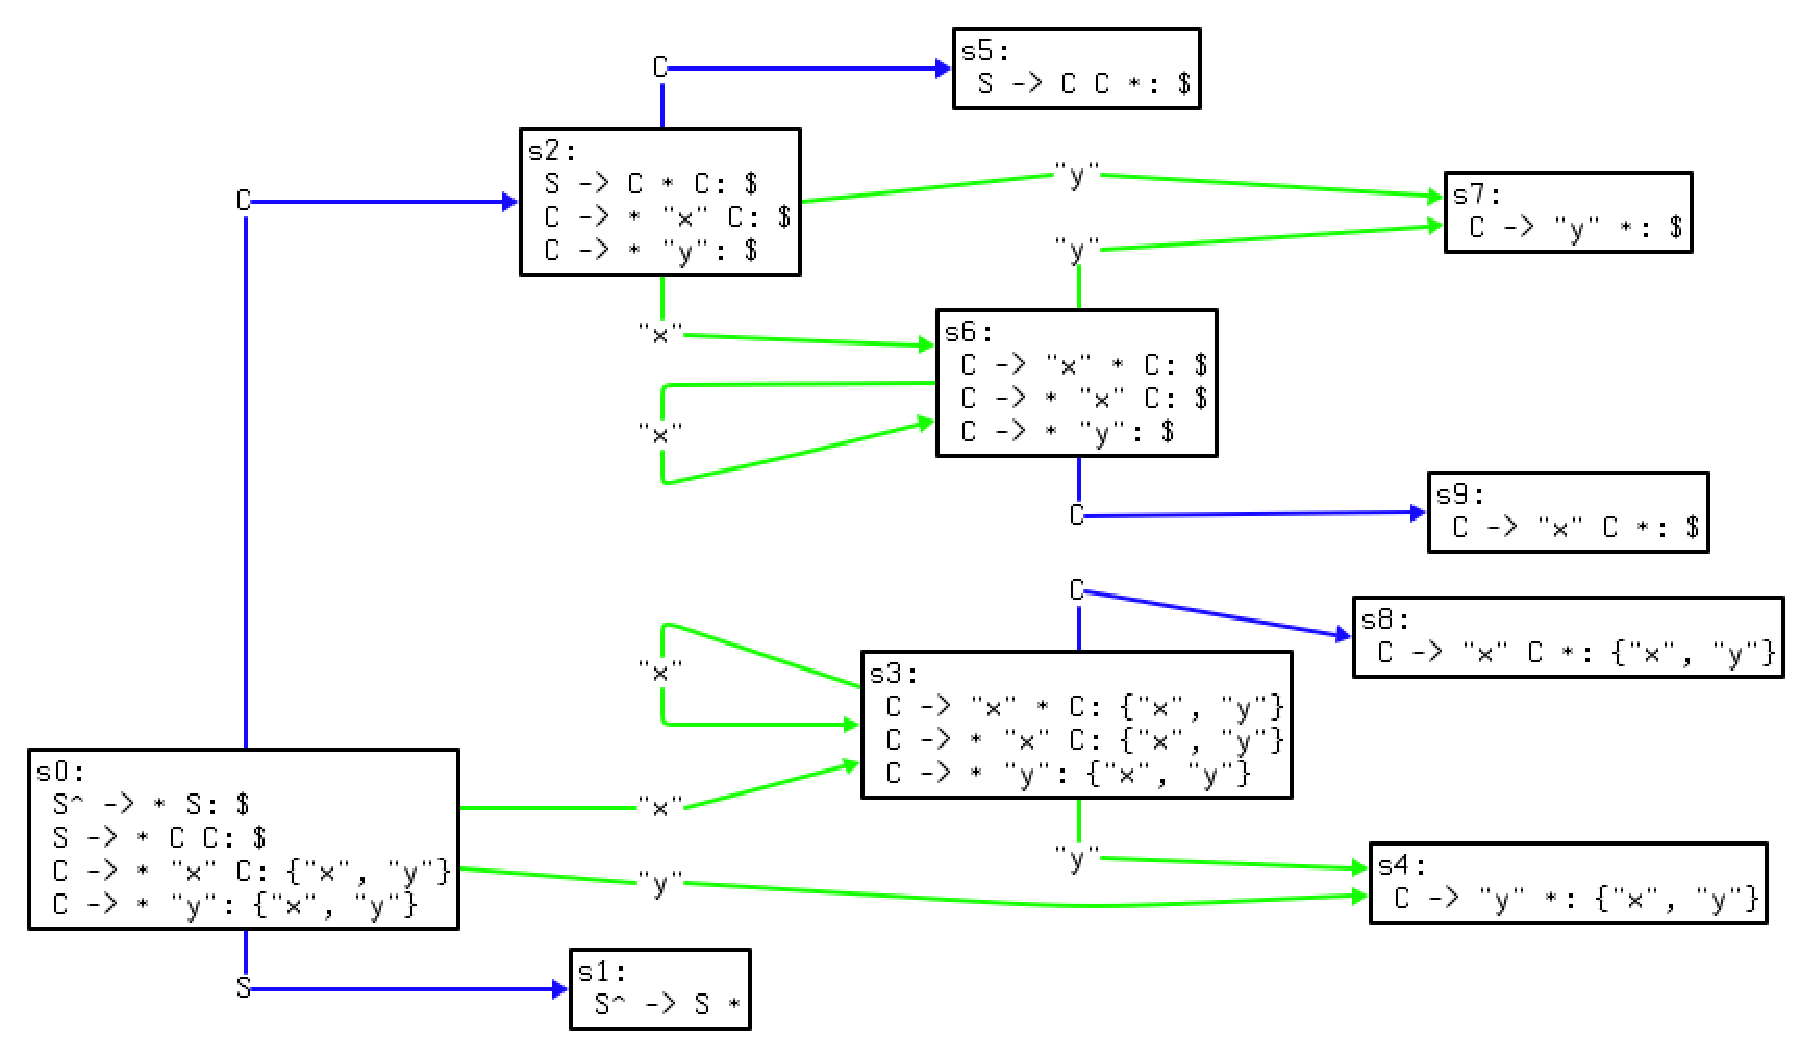
\epsfig{file=Abbildungen/cc-LR.eps, scale=0.5}
      \caption{LR-Goto-Graph f�r die Grammatik aus Abbildung \ref{fig:dragon-book.grammar}.}
  \label{fig:cc-LR.eps}
\end{figure}


Abbildung \ref{fig:cc-LR.eps} zeigt den sogenannten \emph{LR-Goto-Graphen} f�r diese Grammatik.
Die Knoten dieses Graphen sind die Zust�nde.  
Betrachten wir den LR-Goto-Graphen, so stellen wir fest, dass die Zust�nde $s_6$ und
$s_3$ sich nur in den Mengen der Folge-Token unterscheiden, denn es gilt einerseits
\\[0.2cm]
\hspace*{1.3cm}
$s_6 = \Bigl\{ s \rightarrow \squoted{x} \bullet c: \squoted{\symbol{36}}, 
                 c \rightarrow \bullet\, \quoted{x} c:  \squoted{\symbol{36}},
                 c \rightarrow \bullet\, \quoted{y}:    \squoted{\symbol{36}}
       \Bigr\}$, 
\\[0.2cm]
und andererseits haben wir
\\[0.2cm]
\hspace*{1.3cm}
$s_3 = \Bigl\{ s \rightarrow \squoted{x} \bullet c: \{ \squoted{x}, \squoted{y} \}, 
                 c \rightarrow \bullet\, \quoted{x} c:  \{ \squoted{x}, \squoted{y} \},
                 c \rightarrow \bullet\, \quoted{y}:    \{ \squoted{x}, \squoted{y} \}  
       \Bigr\}$.
\\[0.2cm]
Offenbar entsteht die Menge $s_3$ aus der Menge $s_6$ indem �berall $\squoted{\symbol{36}}$
durch die Menge $\{ \squoted{x}, \squoted{y}\}$ ersetzt wird.  Genauso kann die Menge $s_7$ in $s_4$
und $s_9$ in $s_8$ �berf�hrt werden.  Die entscheidende Erkenntnis ist nun, dass die
Funktion $\textsl{goto}()$ unter dieser Art von Transformation invariant ist, denn bei der
Definition dieser Funktion spielt die Menge der Folge-Token keine Rolle.  So sehen wir zum
Beispiel, dass einerseits
\\[0.2cm]
\hspace*{1.3cm}
$\textsl{goto}(s_3, c) = s_8$ \quad und \quad und 
$\textsl{goto}(s_6, c) = s_9$ 
\\[0.2cm]
gilt und dass andererseits der Zustand $s_9$ in den Zustand $s_8$ �bergeht, wenn wir
�berall in $s_9$ das Terminal $\squoted{\symbol{36}}$ durch die Menge 
 $\{ \squoted{x}, \squoted{y}\}$ ersetzen.  Definieren wir den \emph{Kern}
einer Menge von erweiterten markierten Regeln dadurch, dass wir in jeder Regel die Menge
der Folgetoken wegstreichen, und fassen dann Zust�nde mit dem selben Kern zusammen, so
erhalten wir den in 
Abbildung \ref{fig:cc-LALR.eps} gezeigten Goto-Graphen.

\begin{figure}[!ht]
\centering
  \hspace*{-0.6cm} 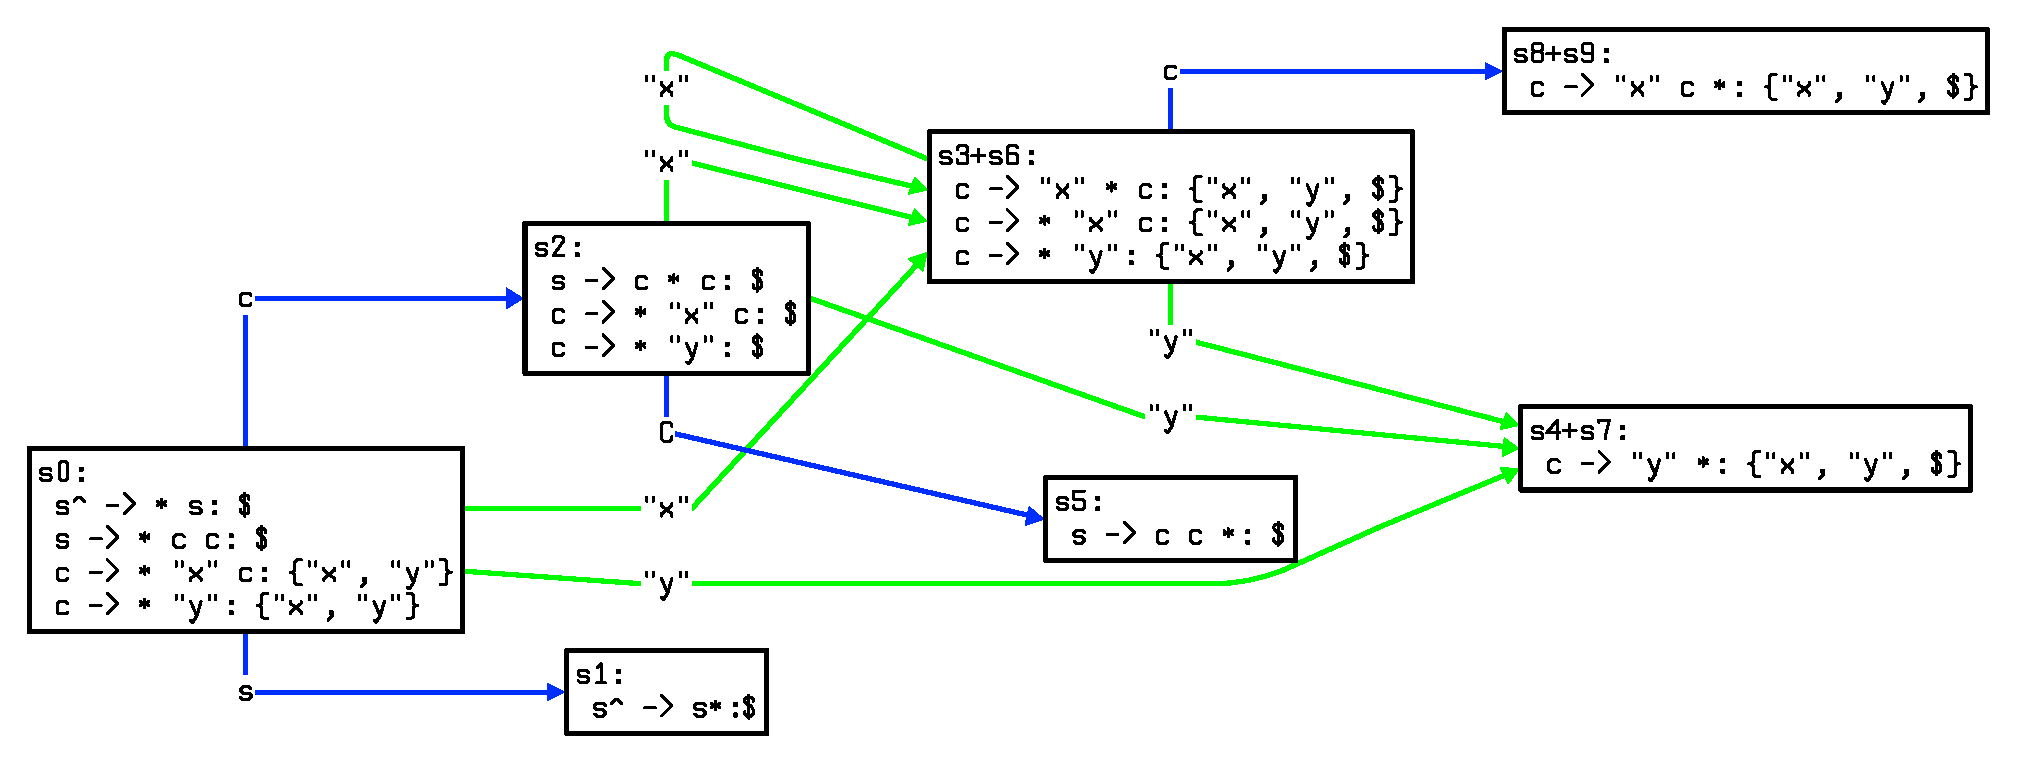
\epsfig{file=Abbildungen/cc-LALR, scale=0.5}
  \caption{Der LALR-Goto-Graph f�r die Grammatik aus Abbildung \ref{fig:dragon-book.grammar}.}
  \label{fig:cc-LALR.eps}
\end{figure}

Um die Beobachtungen, die wir bei der Betrachtung der in Abbildung
\ref{fig:dragon-book.grammar} gezeigten Grammatik gemacht gaben, verallgemeinern und formalisieren zu
k�nnen, definieren wir ein Funktion 
$\textsl{core}()$, die den Kern einer Menge von e.m.R.s berechnet und damit diese Menge in
eine Menge markierter Regeln �berf�hrt: 
\\[0.2cm]
\hspace*{1.3cm}
$\textsl{core}(\mathcal{M}) := 
   \{ a \rightarrow \beta \bullet \gamma \mid (a \rightarrow \beta \bullet \gamma:L) \in \mathcal{M} \}$. 
\\[0.2cm]
Die Funktion $\textsl{core}()$ entfernt also einfach die Menge der Folge-Tokens von den e.m.R.s.
Wir hatten die Funktion $\textsl{goto}()$ f�r eine Menge $\mathcal{M}$ von erweiterten
markierten Regeln und ein Symbol $x$ durch
\\[0.2cm]
\hspace*{1.3cm}
$\textsl{goto}(\mathcal{M}, x) := \textsl{closure}\Bigl( \bigl\{ 
 a \rightarrow \beta\, x \bullet \gamma:L \mid (a \rightarrow \beta \bullet x\, \gamma:L) \in \mathcal{M} 
 \bigr\} \Bigr)
$.
\\[0.2cm]
definiert.  Offenbar spielt die Menge der Folge-Token bei der Berechnung von
$\textsl{goto}(\mathcal{M}, x)$ keine Rolle, formal gilt f�r zwei e.m.R.-Mengen
$\mathcal{M}_1$ und $\mathcal{M}_2$ und ein Symbol $x$ die Formel:
\\[0.2cm]
\hspace*{1.3cm}
$\textsl{core}(\mathcal{M}_1) = \textsl{core}(\mathcal{M}_2) \;\Rightarrow\;
 \textsl{core}(\textsl{goto}(\mathcal{M}_1, x)) = 
 \textsl{core}(\textsl{goto}(\mathcal{M}_2, x))
$.
\vspace*{0.2cm}

F�r zwei e.m.R.-Mengen $\mathcal{M}$ und $\mathcal{N}$, die
den gleichen Kern haben, definieren wir die \emph{erweiterte Vereinigung}  
$\mathcal{M} \uplus \mathcal{N}$ von $\mathcal{M}$ und $\mathcal{N}$ als
\\[0.2cm]
\hspace*{1.3cm}
$\mathcal{M} \uplus \mathcal{N} := 
   \{ a \rightarrow \beta\bullet \gamma:K \cup L \mid 
      (a \rightarrow \beta\bullet \gamma:K) \in \mathcal{M} \;\wedge\;
      (a \rightarrow \beta\bullet \gamma:L) \in \mathcal{N}
   \}
$.
\\[0.2cm] 
Diese Definition verallgemeinern wir zu einer Operation $\biguplus$, 
die auf einer Menge von Mengen von e.m.R.s definiert ist: Ist $\frak{I}$
eine Menge von Mengen von e.m.R.s, die alle den gleichen Kern haben, gilt also
\[ \frak{I} = \{ \mathcal{M}_1, \cdots, \mathcal{M}_k \} \quad \mbox{mit} \quad
   \textsl{core}(\mathcal{M}_i) = \textsl{core}(\mathcal{M}_j) \quad 
   \mbox{f�r alle $i,j\in\{1,\cdots,k\}$,} 
\]
so definieren wir
\[ \biguplus \frak{I} := \mathcal{M}_1 \uplus \cdots \uplus \mathcal{M}_k. 
\]
Es sei nun $\Delta$ die Menge aller Zust�nde eines LR-Parsers.  Dann ist die Menge der Zust�nde des
entsprechenden LALR-Parsers durch die erweiterte Vereinigung der Menge aller der Teilmengen 
von $\Delta$ gegeben, deren Elemente den gleichen Kern haben:
\[ \frak{Q} := \left\{ \biguplus \frak{I} \mid \frak{I} \in 2^\Delta \wedge 
      \forall \mathcal{M},\mathcal{N} \in \frak{I}: \textsl{core}(\mathcal{M}) = \textsl{core}(\mathcal{N}) 
      \wedge \mbox{und $\frak{I}$ maximal} 
   \right\}. 
\]
Die Forderung ``$\frak{I}$ maximal'' dr�ckt in der obigen Definition aus, dass in $\frak{I}$ tats�chlich
\underline{alle} Mengen aus $\Delta$ zusamengefasst sind, die den selben Kern haben.
Die so definierte Menge $\frak{Q}$ ist die Menge der LALR-Zust�nde.  

Als n�chstes �berlegen wir, wie sich die Berechnung von $\textsl{goto}(\mathcal{M},X)$
�ndern muss, wenn $\mathcal{M}$ ein Element der Menge $\frak{Q}$ der LALR-Zust�nde ist.  
Zur Berechnung von $\textsl{goto}(\mathcal{M},X)$ berechnen wir zun�chst die Menge
\\[0.2cm]
\hspace*{1.3cm}
$\textsl{closure}\Bigl( \bigl\{  
  A \rightarrow \alpha X \bullet \beta:L \mid (A \rightarrow \alpha \bullet X \beta:L) \in \mathcal{M} 
  \bigr\} \Bigr)
$.
\\[0.2cm]
Das Problem ist, dass diese Menge im Allgemeinen kein Element der Menge $\frak{Q}$ ist,
denn die Zust�nde in $\frak{Q}$ entstehen ja durch die Zusammenfassung mehrerer LR-Zust�nde.
Die Zust�nde, die bei der Berechnung von $\frak{Q}$ zusammengefasst werden, haben aber alle den selben
Kern.  Daher enth�lt die  Menge
\\[0.2cm]
\hspace*{1.3cm}
$\Bigl\{ q \in \frak{Q} \mid \textsl{core}(q) =
  \textsl{core}\bigl(\textsl{closure}\bigl( \bigl\{  
  a \rightarrow \beta\, x \bullet \gamma:L \mid (a \rightarrow \beta \bullet x\, \gamma:L) \in \mathcal{M} 
  \bigr\} \bigr)\bigr)
  \Bigr\}
$
\\[0.2cm]
genau ein Element und dieses Element ist der Wert von $\textsl{goto}(\mathcal{M}, X)$.  Folglich
k�nnen wir  
\\[0.2cm]
\hspace*{1.3cm}
$\textsl{goto}(\mathcal{M}, X) := \textsl{arb}\Bigl(\Bigl\{ q \in \frak{Q} \mid \textsl{core}(q) =
  \textsl{core}\bigl(\textsl{closure}\bigl( \bigl\{  
  a \rightarrow \beta\, x \bullet \gamma:L \mid (a \rightarrow \beta \bullet x\, \gamma:L) \in \mathcal{M} 
  \bigr\} \bigr)\bigr)
  \Bigr\} \Bigr)
$
\\[0.2cm]
setzen.  Die hier verwendete Funktion $\textsl{arb}()$ dient dazu, ein beliebiges Element aus einer Menge
zu extrahieren.  Da die Menge, aus der hier das Element extrahiert wird, genau ein Element enth�lt, ist
$\textsl{goto}(\mathcal{M}, x)$ wohldefiniert.
Die Berechnung des Ausdrucks $\textsl{action}(\mathcal{M}, t)$ �ndert sich gegen�ber der Berechnung f�r
einen LR-Parser nicht. 

\section{Vergleich von SLR-, LR- und LALR-Parsern}
Wir wollen nun die verschiedenen Methoden, mit denen wir in diesem Kapitel
Shift-Reduce-Parser konstruiert haben, vergleichen.  Wir nennen eine Sprache $\mathcal{L}$
eine \emph{SLR-Sprache}, wenn $\mathcal{L}$ von einem SLR-Parser erkannt werden kann.
Die Begriffe \emph{kanonische LR-Sprache} und \emph{LALR-Sprache} werden analog definiert.
 Zwischen diesen Sprachen bestehen die folgende Beziehungen:
\\[0.2cm]
\hspace*{1.3cm}
\emph{SLR-Sprache} $\subsetneq$ \emph{LALR-Sprache} $\subsetneq$ \emph{kanonische LR-Sprache} 
\hspace*{\fill} $(\star)$
\\[0.2cm]
Diese Inklusionen sind leicht zu verstehen:  Bei der Definition der LR-Parser hatten wir
zu den markierten Regeln  Mengen von Folge-Token hinzugef�gt.  Dadurch war
es m�glich, in bestimmten F�llen Shift-Reduce- und Reduce-Reduce-Konflikte zu vermeiden.
Da die Zustands-Mengen der kanonischen LR-Parser unter Umst�nden sehr gro� werden k�nnen,
hatten wir dann wieder solche Mengen von erweiterten markierten Regeln zusammengefasst,
f�r die die Menge der Folge-Token identisch war.  So hatten wir die LALR-Parser
erhalten.  Durch die Zusammenfassung von Regel-Menge k�nnen wir
uns allerdings in bestimmten F�llen Reduce-Reduce-Konflikte einhandeln, so dass die 
Menge der LALR-Sprachen eine Untermenge der kanonischen LR-Sprachen ist.

Wir werden in den folgenden Unterabschnitten zeigen, dass die Inklusionen in $(\star)$ echt sind.  

\subsection{\emph{SLR-Sprache} $\subsetneq$ \emph{LALR-Sprache}}
Die Zust�nde eines LALR-Parsers enthalten gegen�ber den Zust�nden eines SLR-Parsers noch
Mengen von Folge-Token.  Damit sind LALR-Parser mindestens genauso m�chtig wie SLR-Parser.
Wir zeigen nun, dass LALR-Parser tats�chlich m�chtiger als SLR-Parser sind.  Um diese
Behauptung zu belegen, pr�sentieren wir eine Grammatik, f�r die es zwar einen LALR-Parser,
aber keinen SLR-Parser gibt.  Wir hatten auf Seite \pageref{fig:reduce-reduce-conflict.grammar}
gesehen, dass die Grammatik
\\[0.2cm]
\hspace*{1.3cm}
$s \;\rightarrow\; a \quoted{x} a \quoted{y} \mid b \quoted{y} b \quoted{x}$, \quad
$a \;\rightarrow\;\varepsilon$, \quad
$b \;\rightarrow\; \varepsilon$
\\[0.2cm]
keine SLR-Grammatik ist.  Sp�ter hatten wir gesehen, dass diese Grammatik von einem
kanonischen LR-Parser geparst werden kann.  Wir zeigen nun, dass diese Grammatik auch von
einem LALR-Parser geparst werden kann.  Dazu berechnen wir die Menge der LALR-Zust�nde.
Dazu ist zun�chst die Menge der kanonischen LR-Zust�nde zu berechnen.  Diese Berechnung
hatten wir bereits fr�her durchgef�hrt und dabei die folgenden Zust�nde erhalten:
\begin{enumerate}
\item $s_0  = \bigl\{ \widehat{s} \rightarrow \bullet\, s:\symbol{36},
                     s \rightarrow \bullet\, a \squoted{x} a \squoted{y}:\symbol{36},
                     s \rightarrow \bullet\, b \squoted{y} b \squoted{x}:\symbol{36},
                     a \rightarrow \bullet\,: \squoted{x},
                     b \rightarrow \bullet\,: \squoted{y}
              \bigr\}
      $,
\item $s_1 = \bigl\{ s \rightarrow a \bullet \squoted{x} a \squoted{y}:\symbol{36} \bigr\}$,
\item $s_2 = \bigl\{ \widehat{s} \rightarrow s \bullet:\symbol{36} \bigr\}$,
\item $s_3 = \bigl\{ s \rightarrow b \bullet \squoted{y} b \squoted{x}: \symbol{36} \bigr\}$,
\item $s_4 = \bigl\{ s \rightarrow b \squoted{y} \bullet b \squoted{x}: \symbol{36},
                     b \rightarrow \bullet\,: \squoted{x}
             \bigr\}
      $,
\item $s_5 = \bigl\{ s \rightarrow b \squoted{y} b \bullet \squoted{x}: \symbol{36} \bigr\}$,
\item $s_6 = \bigl\{ s \rightarrow b \squoted{y} b \squoted{x} \bullet: \symbol{36} \bigr\}$,
\item $s_7 = \bigl\{ s \rightarrow a \squoted{x} \bullet a \squoted{y}:\symbol{36},
                     a \rightarrow \bullet\,: \squoted{y}
              \bigr\}
      $,
\item $s_8 = \bigl\{ s \rightarrow a \squoted{x} a \bullet \squoted{y}:\symbol{36} \bigr\}$,
\item $s_9 = \bigl\{ s \rightarrow a \squoted{x} a \squoted{y} \bullet :\symbol{36} \bigr\}$.
\end{enumerate}
Wir stellen fest, dass die Kerne aller hier aufgelisteten Zust�nde verschieden sind.
Damit stimmt bei dieser Grammatik die Menge der Zust�nde des LALR-Parser mit der Menge der
Zust�nde des kanonischen LR-Parsers �berein.  Daraus folgt, dass es auch bei
den LALR-Zust�nden keine Konflikte gibt, denn beim �bergang von kanonischen LR-Parsern zu
LALR-Parsern haben wir lediglich Zust�nde mit gleichem Kern zusammengefasst, die
Definition der Funktionen $\textsl{goto}()$ und $\textsl{action}()$ blieb unver�ndert.

\subsection{\emph{LALR-Sprache} $\subsetneq$ \emph{kanonische LR-Sprache}}
Wir hatten LALR-Parser dadurch definiert, dass wir verschiedene Zust�nde eines kanonischen LR-Parsers
zusammengefasst haben.  Damit ist klar, dass kanonische LR-Parser mindestens so m�chtig
sind wie LALR-Parser.  Um zu zeigen, dass kanonische LR-Parser tats�chlich m�chtiger sind
als LALR-Parser, ben�tigen wir eine Grammatik, f�r die sich zwar ein kanonischer LR-Parser,
aber kein LALR-Parser erzeugen l�sst.  Abbildung \ref{fig:lr-but-notlalr.g} zeigt eine
solche Grammatik, die ich dem Drachenbuch entnommen habe.

\begin{figure}[htbp]
  \begin{center}    
  \framebox{
  \framebox{
  \begin{minipage}[t]{5.5cm}
    \vspace*{-0.3cm}

  \begin{eqnarray*}
  s  & \rightarrow & \quoted{v} a \quoted{y} \\
     & \mid        & \quoted{w} b \quoted{y} \\
     & \mid        & \quoted{v} b \quoted{z} \\
     & \mid        & \quoted{w} a \quoted{z} \\[0.1cm]
  a  & \rightarrow & \quoted{x}              \\[0.1cm]
  b  & \rightarrow & \quoted{x}              
  \end{eqnarray*}
  \vspace*{-0.5cm}

  \end{minipage}}}
  \vspace*{-0.3cm}

  \end{center}
  \caption{Eine kanonische LR-Grammatik, die keine LALR-Grammatik ist.}
  \label{fig:lr-but-notlalr.g}
\end{figure}

Wir berechnen zun�chst die Menge der Zust�nde eines kanonischen LR-Parsers f�r diese
Grammatik.  Wir erhalten dabei die folgende Mengen von erweiterten markierten Regeln:
\begin{enumerate}
\item $s_0 = \textsl{closure}(\widehat{s} \rightarrow \bullet\, \;s: \symbol{36}) =
       \{
       \begin{array}[t]{lcl}
         \widehat{s} & \rightarrow & \bullet \;s: \symbol{36},                \\
         s           & \rightarrow & \bullet \squoted{v} a \squoted{y}: \symbol{36}, \\
         s           & \rightarrow & \bullet \squoted{v} b \squoted{z}: \symbol{36}, \\
         s           & \rightarrow & \bullet \squoted{w} a \squoted{z}: \symbol{36}, \\
         s           & \rightarrow & \bullet \squoted{w} b \squoted{y}: \symbol{36}\;\},
        \end{array}
       $
\item $s_1 = \textsl{goto}(s_0, s) =\{ \widehat{s} \rightarrow s \bullet: \symbol{36} \}$
\item $s_2 = \textsl{goto}(s_0, \quoted{v}) = \{ 
       \begin{array}[t]{lcl}
        s & \rightarrow & \squoted{v} \bullet b \squoted{z}: \symbol{36}, \\
        s & \rightarrow & \squoted{v} \bullet a \squoted{y}: \symbol{36}, \\
        a & \rightarrow & \bullet \squoted{x}: \squoted{y}, \\
        b & \rightarrow & \bullet \squoted{x}: \squoted{z}\; \},
       \end{array}
      $
\item $s_3 = \textsl{goto}(s_0, \quoted{w}) = \{ 
       \begin{array}[t]{lcl}
       s & \rightarrow & \squoted{w} \bullet a \squoted{z}: \symbol{36},  \\
       s & \rightarrow & \squoted{w} \bullet b \squoted{y}: \symbol{36},  \\
       a & \rightarrow & \bullet \squoted{x}: \squoted{z},                \\
       b & \rightarrow & \bullet \squoted{x}: \squoted{y}\; \},
       \end{array}
      $
\item $s_4 = \textsl{goto}(s_2, \quoted{x}) =
             \{ a \rightarrow \squoted{x} \bullet: \squoted{y},\;
                b \rightarrow \squoted{x} \bullet: \squoted{z} \}$,
\item $s_5 = \textsl{goto}(s_3, \quoted{x}) =
             \{ a \rightarrow \squoted{x} \bullet: \squoted{z},\,
                b \rightarrow \squoted{x} \bullet: \squoted{y} \}$,
\item $s_6 = \textsl{goto}(s_2, a) =
             \{ s \rightarrow \squoted{v} a \bullet \squoted{y}: \symbol{36} \}$,
\item $s_7 = \textsl{goto}(s_6, \quoted{y}) =
             \{ s \rightarrow \squoted{v} a \squoted{y} \bullet: \symbol{36} \}$,
\item $s_8 = \textsl{goto}(s_2, b) =
             \{ s \rightarrow \squoted{v} b \bullet \squoted{z}: \symbol{36} \}$,
\item $s_9 = \textsl{goto}(s_8, \quoted{z}) =
             \{ s \rightarrow \squoted{v} b \squoted{z} \bullet: \symbol{36} \}$,
\item $s_{10} = \textsl{goto}(s_3, a) =
                \{ s \rightarrow \squoted{w} a \bullet \squoted{z}: \symbol{36} \}$,
\item $s_{11} = \textsl{goto}(s_{10}, \quoted{z}) =
                \{ s \rightarrow \squoted{w} a \squoted{z} \bullet: \symbol{36} \}$,
\item $s_{12} = \textsl{goto}(s_3, b) =
                \{ s \rightarrow \squoted{w} b \bullet \squoted{y}: \symbol{36} \}$,
\item $s_{13} = \textsl{goto}(s_{12}, \quoted{y}) =
                \{ s \rightarrow \squoted{w} b \squoted{y} \bullet: \symbol{36} \}$.
\end{enumerate}
Die einzigen Zust�nde, bei denen es Konflikte geben k�nnte, sind die Mengen $s_4$ und
$s_5$, denn hier sind prinzipiell sowohl Reduktionen mit der Regel
\\[0.2cm]
\hspace*{1.3cm}
$a \rightarrow \squoted{x}$ \quad als auch mit \quad
$b \rightarrow \squoted{x}$
\\[0.2cm]
m�glich.  Da allerdings die Mengen der Folge-Token einen leeren Durchschnitt haben, gibt
es tats�chlich keinen Konflikt und die Grammatik ist eine kanonische LR-Grammatik.

Wir berechnen als n�chstes die LALR-Zust�nde der oben angegebenen Grammatik.  Die einzigen
Zust�nde, die einen gemeinsamen Kern haben, sind die beiden Zust�nde $s_4$ und $s_5$, denn
es gilt
\\[0.2cm]
\hspace*{1.3cm}
$\textsl{core}(s_4) = \{ a \rightarrow \squoted{x} \bullet,\;
                b \rightarrow \squoted{x} \bullet \} = \textsl{core}(s_5)$.
\\[0.2cm]
Bei der Berechnung der LALR-Zust�nde werden diese beiden Zust�nde zu einem Zustand
$s_{\{4,5\}}$ zusammengefasst.  Dieser neue Zustand hat die Form
\\[0.2cm]
\hspace*{1.3cm}
$s_{\{4,5\}} = \bigl\{ A \rightarrow \squoted{x} \bullet: \{\squoted{y}, \squoted{z} \},\;
                       B \rightarrow \squoted{x} \bullet: \{\squoted{y}, \squoted{z} \} \bigr\}$.
\\[0.2cm]
Hier gibt es offensichtlich  einen Reduce-Reduce-Konflikt, denn einerseits haben wir
\\[0.2cm]
\hspace*{1.3cm}
$\textsl{action}(s_{\{4,5\}}, \squoted{y}) = \pair(\textsl{reduce}, A \rightarrow \squoted{x})$,
\\[0.2cm]
andererseits gilt aber auch
\\[0.2cm]
\hspace*{1.3cm}
$\textsl{action}(s_{\{4,5\}}, \squoted{y}) = \pair(\textsl{reduce}, B \rightarrow \squoted{x})$.

\exercise
Es sei $G = \langle V, T, R, s \rangle$ eine LR-Grammatik,
Es sei $\mathcal{M}$ die Menge der LR-Zust�nde dieser Grammatik und $\mathcal{N}$ sei die Menge der
LALR-Zust�nde der Grammatik.  �berlegen Sie, warum es in der Menge $\mathcal{N}$ keine
Shift-Reduce-Konflikte geben kann.  \eox


\paragraph{Historical Notes}
The theory of LALR parsing is due to Franklin L.~DeRemer \cite{deRemer:71}.  At the time of its
invention,  the space savings of LALR parsing in comparison to LR parsing were crucial.  


\subsection{Bewertung der verschiedenen Methoden}
F�r die Praxis sind SLR-Parser nicht ausreichend, denn es gibt eine Reihe praktisch
relevanter Sprach-Konstrukte, f�r die sich kein SLR-Parser erzeugen l�sst.  Kanonische
LR-Parser sind wesentlich m�chtiger, ben�tigen allerdings oft deutlich mehr Zust�nde. 
Hier stellen LALR-Parser einen Kompromiss dar:  Einerseits sind LALR-Sprachen fast so
ausdrucksstark  wie kanonische LR-Sprachen, andererseits liegt der Speicherbedarf von
LALR-Parsern in der gleichen Gr��enordnung wie der Speicherbedarf von SLR-Parsern.  Beispielsweise
hat die SLR-Parse-Tabelle f�r die Sprache \texttt{C} insgesamt 349 Zust�nde, die entsprechende
LR-Parse-Tabelle kommt auf 1572 Zust�nde, w�hrend der LALR-Parser mit 350 Zust�nden auskommt und damit nur
einen Zustand mehr als der SLR-Parser hat.  
In den heute in der Regel zur Verf�gung stehenden Hauptspeichern lassen sich allerdings
auch kanonische LR-Parser meist m�helos unterbringen, so dass es eigentlich keinen zwingenden
Grund mehr gibt, statt eines LR-Parsers einen LALR-Parser einzusetzen.  

Andererseits wird niemand einen LALR-Parser oder einen kanonischen LR-Parser von Hand
programmieren wollen.  Statt dessen werden Sie sp�ter einen Parser-Generator wie \textsl{Bison}
oder \textsl{JavaCup} einsetzen, der Ihnen einen  Parser generiert.  Das Werkzeug Bison
ist ein Parser-Generator f�r \texttt{C}, \texttt{C++} und bietet auch eine, allerdings leider noch
experimentelle, Unterst�tzung f�r \textsl{Java},
w�hrend \textsl{JavaCup} auf die Sprache \textsl{Java} beschr�nkt ist.  Falls Sie
\textsl{JavaCup} benutzen, haben Sie keine Wahl, denn dieses Werkzeug erzeugt immer einen
LALR-Parser.  Bei \href{http://www.gnu.org/software/bison/manual/bison.html}{\textsl{Bison}} ist es
ab der Version 3.0  auch m�glich, einen LR-Parser zu erzeugen.



%%% Local Variables: 
%%% mode: latex
%%% TeX-master: "formal-languages"
%%% End: 

%\section{Erzeugung von LALR-Parsern mit \textsl{Bison}}
Die von dem Parser-Generator \textsl{Bison} erzeugten Parser sind LALR-Parser.
\textsl{Bison} bietet die M\"oglichkeit, die erzeugten Mengen von e.m.R.s textuell oder
grafisch darzustellen.  Abbildung \ref{fig:cc.y} zeigt, wie die Grammatik aus Abbildung
\ref{fig:dragon-book.grammar} als Eingabe-Datei f\"ur \textsl{Bison} formatiert werden kann.
Da es uns hier nur um die Erzeugung der Zustands-Mengen geht, enth\"alt die Datei weder
Deklarationen, die zur Anbindung eines Scanners erfoderlich w\"aren, noch semantische Aktionen.

\begin{figure}[!ht]
\centering
\begin{Verbatim}[ frame         = lines, 
                  framesep      = 0.3cm, 
                  labelposition = bottomline,
                  numbers       = left,
                  numbersep     = -0.2cm,
                  xleftmargin   = 0.8cm,
                  xrightmargin  = 0.8cm,
                ]
    %%
    S : C C;
    
    C : 'x' C
      | 'y'
      ;     
    %%
\end{Verbatim}
\vspace*{-0.3cm}
\caption{Die Grammatik aus Abbildung \ref{fig:dragon-book.grammar} im \textsl{Bison}-Format.}
\label{fig:cc.y}
\end{figure}

\noindent
\"Ubersetzen wir die in Abbildung \ref{fig:cc.y} gezeigte Datei mit dem Befehl
\[ \texttt{bison -v -g cc.y} \]
so werden von \textsl{Bison} zwei Dateien erzeugt:
\begin{enumerate}
\item Die Option ``\texttt{-v}'' (\emph{verbose}) bewirkt, dass die Datei
      \texttt{cc.output} erzeugt wird.  Diese Datei enth\"alt die Zust\"ande des
      LALR-Parsers und wird in Abbildung \ref{fig:cc.output} gezeigt.
\item Die Option ``\texttt{-g}'' (\emph{graphic}) erzeugt die Datei
      \texttt{cc.vcg}.  Die Datei-Endung \texttt{.vcg} steht als Abk\"urzung f\"ur 
      \emph{visualization of compiler graphs}.
      Diese Datei stellt den Goto-Graphen der Grammatik im
      \emph{VCG-Format} dar und l\"asst sich mit Hilfe geeigneter Werkzeuge grafisch
      darstellen.  
      Ein solches Werkzeug ist \texttt{aiSee}, dass Sie im Internet unter der Adresse
      \\[0.2cm]
      \hspace*{1.3cm}
      \texttt{http://www.aisee.com/}
      \\[0.2cm]
      finden.  Dort k\"onnen Sie eine Demoversion kostenlos herunterladen.
\end{enumerate}

\begin{figure}[!ht]
\centering
\begin{Verbatim}[ frame         = lines, 
                  framesep      = 0.3cm, 
                  labelposition = bottomline,
                  numbers       = left,
                  numbersep     = -0.2cm,
                  xleftmargin   = 0.8cm,
                  xrightmargin  = 0.8cm,
                ]
    Grammar
        0 $accept: S $end
        1 S: C C
        2 C: 'x' C
        3  | 'y'
    Terminals, with rules where they appear
    $end (0) 0
    'x' (120) 2
    'y' (121) 3
    error (256)
    Nonterminals, with rules where they appear
    $accept (5)
        on left: 0
    S (6)
        on left: 1, on right: 0
    C (7)
        on left: 2 3, on right: 1 2
    state 0
        0 $accept: . S $end
        'x'  shift, and go to state 1
        'y'  shift, and go to state 2
        S  go to state 3
        C  go to state 4
    state 1
        2 C: 'x' . C
        'x'  shift, and go to state 1
        'y'  shift, and go to state 2
        C  go to state 5
    state 2
        3 C: 'y' .
        $default  reduce using rule 3 (C)
    state 3
        0 $accept: S . $end
        $end  shift, and go to state 6
    state 4
        1 S: C . C
        'x'  shift, and go to state 1
        'y'  shift, and go to state 2
        C  go to state 7
    state 5
        2 C: 'x' C .
        $default  reduce using rule 2 (C)
    state 6
        0 $accept: S $end .
        $default  accept
    state 7
        1 S: C C .
        $default  reduce using rule 1 (S)
\end{Verbatim}
%$
\vspace*{-0.3cm}
\caption{Die Datei \texttt{cc.output}.}
\label{fig:cc.output}
\end{figure} 

Wir diskutieren nun die in Abbildung \ref{fig:cc.output} gezeigte Datei \texttt{cc.output}
Zeile f\"ur Zeile.
\begin{enumerate}
\item Die Zeilen 1 -- 5 zeigen die zu Grunde liegende Grammatik.  Die 0-te Regel hat hier
      die Form
      \\[0.2cm]
      \hspace*{1.3cm}
      $\texttt{\$accept: S \$end}$
      \\[0.2cm]
      und entspricht im Wesentlichen unserer Regel
      \\[0.2cm]
      \hspace*{1.3cm}
      $\widehat{S} \rightarrow S$,
      \\[0.2cm]
      wobei der String ``\texttt{\$end}''
      %\$
      f\"ur das Ende der Eingabe steht.  Bei Bison wird also das Datei-Ende-Zeichen
      \textsc{Eof} mit zu der Regel hinzugenommen.

      Wie Sie sehen, sind die einzelnen Grammatik-Regeln mit 0 beginnend numeriert.
      Auf diese Nummerierung wird  Bezug genommen.
\item Die Zeilen 7 -- 10 listen alle Terminale auf, die in der Grammatik verwendet
      werden.  Die Zeile
      \\[-0.2cm]
      \hspace*{1.3cm}
      $\texttt{'x' (120) 2}$
      \\[0.2cm]
      ist beispielsweise wie folgt zu lesen:
      \begin{enumerate}
      \item \texttt{'x'} ist ein Terminal
      \item mit dem \textsc{Ascii}-Code 120 und
      \item dieses Terminal tritt in der Regel 2 auf.
      \end{enumerate}
      Neben den vom Benutzer in der Grammatik definierten Terminalen ``\texttt{x}'' und
      ``\texttt{y}'' f\"uhrt \textsl{Bison} noch die beiden Terminale
      ``\texttt{\symbol{36}end}'' und ``\texttt{error}'' ein.  Ersteres bezeichnet das
      Ende der Eingabe, letzteres steht f\"ur ein Token, dass nicht in der Eingabe-Sprache vorkommt.
\item Die Zeilen 11 -- 17 listen die syntaktischen Variable, die hier als Nicht-Terminale
      bezeichnet werden, auf und geben die Regeln an, wo diese Variablen auftreten.
      Auch den Variablen werden Zahlen zugeordnet.  Diese Zahlen spielen jedoch nur
      in dem Code des von Bison erzeugten Parsers eine Rolle.
\item Der Rest der Datei zeigt die Zust\"ande und spezifiziert gleichzeitig die Funktionen
      $\textsl{goto}()$ und $\textsl{action}()$.  Bei den Zust\"anden wird allerdings nicht
      die gesamte Menge der e.m.R. angegeben, sondern es wird nur eine Menge
      $\textsc{M}^-$ angegeben, aus der sich mit Hilfe der Funktion $\textsl{closure}()$
      die gesamte Menge nach der Formel
      \\[0.2cm]
      \hspace*{1.3cm}
      $\textsc{M} = \textsl{closure}(\textsc{M}^-)$
      \\[0.2cm]
      berechnen l\"asst.  Au{\ss}erdem werden die Mengen der Folge-Token nicht angegeben.
      Wir betrachten nun zwei der Zust\"ande im Detail:
      \begin{enumerate}
      \item Der Zustand ``\texttt{state 1}'', der in der Zeile 25 spezifiziert
            wird, entspricht der Menge
            \\[0.2cm]
            \hspace*{-0.8cm}
            $s_1 = \textsl{closure}(\{ C \rightarrow \quoted{x} \bullet C \})$
            \\[0.1cm]
            Hier ist zu beachten, dass an Stelle des Markierungs-Symbols ``$\bullet$''
            ein Punkt ``\texttt{.}'' verwendet wird.  
            
            In Zeile 26 wird  spezifiziert, dass
            \\[0.2cm]
            \hspace*{1.3cm} 
            $\textsl{goto}(s_1, \squoted{x}) = s_1$ \quad und \quad
            $\textsl{action}(s_1, \squoted{x}) =\langle \texttt{shift}, s_1 \rangle$
            \\[0.2cm]
            gilt.  Analog ist Zeile 27 als
            \\[0.2cm]
            \hspace*{1.3cm} 
            $\textsl{goto}(s_1, \squoted{y}) = s_2$ \quad und \quad
            $\textsl{action}(s_1, \squoted{x}) = \langle \texttt{shift}, s_2 \rangle$
            \\[0.2cm]
            zu lesen und in Zeile 28 haben wir
            \\[0.2cm]
            \hspace*{1.3cm}
            $\textsl{goto}(s_1,C) = s_5$.
      \item Der Zustand ``\texttt{state 2}'', der in der Zeile 30 spezifiziert
            wird, entspricht der Menge
            \\[0.2cm]
            \hspace*{1.3cm}
            $s_2 = \textsl{closure}\bigl(\bigl\{ C \rightarrow \squoted{y} \bullet:  \{
            \squoted{x}, \squoted{y},\symbol{36} \bigr\}\bigr)$.
            \\[0.2cm]
            Zeile 31 ist als
            \\[0.2cm]
            \hspace*{1.3cm}
            $\textsl{action}(s_2,t) = \langle \texttt{reduce}, C \rightarrow \quoted{x} C \rangle$ 
            \quad f\"ur alle Token $t$
            \\[0.2cm]
            zu lesen.
      \end{enumerate}
\end{enumerate}
Neben der eben diskutierten textuellen Darstellung bietet \textsl{Bison} noch die Option, die Zust\"ande des
LALR-Parsers grafisch darzustellen.  Dazu erzeugt \textsl{Bison} zun\"achst die Datei \texttt{cc.vcg}, die dann
beispielsweise mit dem Werkzeug \texttt{aisee} visualsiert werden kann.  Abbildung
\ref{fig:bison-goto-graph.eps} zeigt diese Visualisierung. 

\begin{figure}[!ht]
\centering
      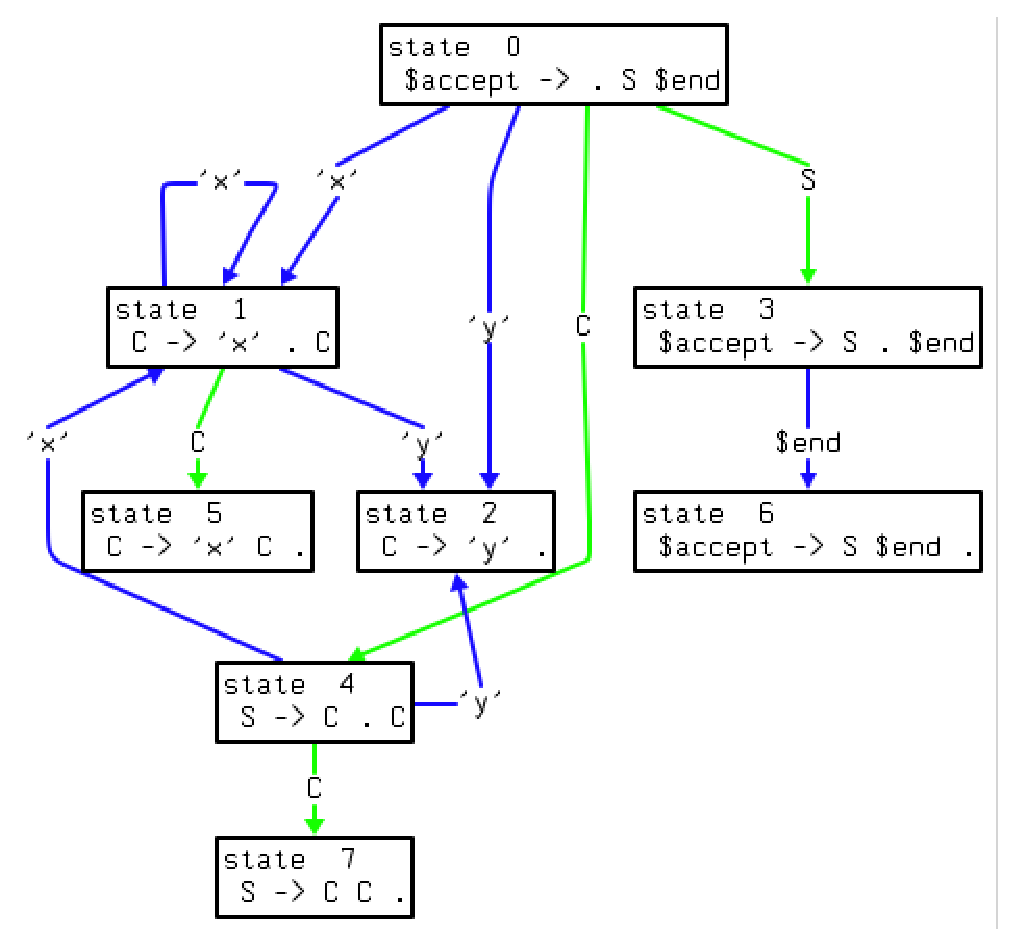
\epsfig{file=Abbildungen/cc-bison, scale=0.5}
  \caption{Von \textsl{Bison} erzeugte grafische Darstellung des Goto-Graphen der Grammatik aus Abbildung \ref{fig:dragon-book.grammar}.}
  \label{fig:bison-goto-graph.eps}
\end{figure}
\pagebreak

\vspace*{\fill}
\pagebreak

\section{Die Behandlung von Konflikten mit \textsl{Bison}}
\textsl{Bison} kann auch dann noch Grammatiken erzeugen, wenn bei der Konstruktion der Zust\"ande Shift-Reduce-
oder Reduce-Reduce-Konflikte auftreten.  Wir besprechen anhand zweier typischer Situationen, wie
\textsl{Bison} in solchen F\"allen vorgeht.

\subsection{Operator-Pr\"azedenzen}
\begin{figure}[!ht]
\centering
\begin{Verbatim}[ frame         = lines, 
                  framesep      = 0.3cm, 
                  labelposition = bottomline,
                  numbers       = left,
                  numbersep     = -0.2cm,
                  xleftmargin   = 0.8cm,
                  xrightmargin  = 0.8cm,
                ]
    %token N
    
    %%
    
    E : E '+' E
      | E '*' E
      | N
      ;
\end{Verbatim}
\vspace*{-0.3cm}
\caption{\textsl{Bison}-Darstellung der Grammatik aus Abbildung \ref{fig:shift-reduce-conflict.grammar}.}
\label{fig:conflict.y}
\end{figure}

\noindent
Wir beginnen mit der in Abbildung \ref{fig:shift-reduce-conflict.grammar} gezeigten Grammatik f\"ur
arithmetische Ausdr\"ucke.  Abbildung \ref{fig:conflict.y} zeigt, wie diese Grammatik sich f\"ur \textsl{Bison}
darstellen l\"asst.   Hier haben wir in Zeile 1 festgelegt, dass ``\texttt{N}'' als Nicht-Terminal zu
interpretieren ist.  \"Ubersetzen wir diese Grammatik mit dem Befehl
\\[0.2cm]
\hspace*{1.3cm}
\texttt{bison -v conflict.y},
\\[0.2cm]
so erhalten wir die Warnung
\\[0.2cm]
\hspace*{1.3cm}
\texttt{conflict.y: conflicts: 4 shift/reduce}.
\\[0.2cm]
Bei der \"Ubersetzung dieser Grammatik sind also insgesamt 4 Shift-Reduce-Konflikte aufgetreten.
Wir wollen diese Konflikte jetzt genauer analysieren und inspizieren zu diesem Zweck die von \textsl{Bison}
erzeugte Datei \texttt{conflict.output}.  Die relevanten Teile dieser Datei sind in Abbildung
\ref{fig:conflict.output} wiedergegeben.  Wir diskutieren diese Datei jetzt im Detail.

\begin{figure}[!ht]
\centering
\begin{Verbatim}[ frame         = lines, 
                  framesep      = 0.3cm, 
                  labelposition = bottomline,
                  numbers       = left,
                  numbersep     = -0.2cm,
                  xleftmargin   = 0.8cm,
                  xrightmargin  = 0.8cm,
                  commandchars  = \\\(\),
                ]
    State 6 conflicts: 2 shift/reduce
    State 7 conflicts: 2 shift/reduce
    
    Grammar
        0 $accept: E $end
        1 E: E '+' E
        2  | E '*' E
        3  | N

        \(\vdots\)

    state 6    
        1 E: E . '+' E
        1  | E '+' E .
        2  | E . '*' E
        '+'  shift, and go to state 4
        '*'  shift, and go to state 5
        '+'       [reduce using rule 1 (E)]
        '*'       [reduce using rule 1 (E)]
        $default  reduce using rule 1 (E)
    state 7
        1 E: E . '+' E
        2  | E . '*' E
        2  | E '*' E .
        '+'  shift, and go to state 4
        '*'  shift, and go to state 5
        '+'       [reduce using rule 2 (E)]
        '*'       [reduce using rule 2 (E)]
        $default  reduce using rule 2 (E)
\end{Verbatim}
\vspace*{-0.3cm}
\caption{Darstellung der Shift-Reduce-Konflikte durch \textsl{Bison}.}
\label{fig:conflict.output}
\end{figure}
\begin{enumerate}
\item Am Anfang der Datei werden alle Konflikte aufgelistet.
      Bei der von \textsl{Bison} \"ubersetzten Grammatik gibt es in den Zust\"anden ``\texttt{state 6}'' 
      und ``\texttt{state 7}'' jeweils zwei 
      Shift-Reduce-Konflikte.
\item Zustand ``\texttt{state 6}'' besteht aus den Regeln 
      \\[0.2cm]
      \hspace*{1.3cm}
      $E \rightarrow E \bullet \quoted{+} E,\quad E \rightarrow E \quoted{+} E \bullet \quad \mbox{und} \quad
       E \rightarrow E \bullet \quoted{*} E$.
      \\[0.2cm]
      Hier gibt es zwei Shift-Reduce-Konflikte.
      \begin{enumerate}
      \item Bei der Berechnung von $\textsl{action}(\texttt{state 6}, \squoted{+})$ gibt es einen
            Shift-Reduce-Konflikt, denn die markierte Regel $E \rightarrow E \bullet \quoted{+} E$
            verlangt, dass das Token $\squoted{+}$ auf den Stack geschoben wird, w\"ahrend die markierte
            Regel $E \rightarrow E \quoted{+} E \bullet$ fordert, dass der Symbolstack mit der Grammatik-Regel 
            $E \rightarrow E \quoted{+} E$ reduziert wird.

            Leider werden die Mengen der Folge-Token bei \textsl{Bison} nicht mit ausgegeben, so dass
            die Tatsache, dass das Token $\squoted{+}$ tats\"achlich ein Folge-Token der markierten Regel
            $E \rightarrow E \quoted{+} E$ ist, aus der von \textsl{Bison} produzierten Ausgabe nicht
            ersichtlich ist.
      \item Bei der Berechnung von $\textsl{action}(\texttt{state 6}, \squoted{*})$ gibt es einen
            Shift-Reduce-Konflikt, denn die markierte Regel $E \rightarrow E \bullet \quoted{*} E$
            verlangt, dass das Token $\squoted{*}$ auf den Stack geschoben wird, w\"ahrend die markierte
            Regel $E \rightarrow E \quoted{+} E \bullet$ fordert, dass der Symbolstack mit der Grammatik-Regel 
            $E \rightarrow E \quoted{+} E$ reduziert wird.
      \end{enumerate}
      In den Zeilen 16 -- 19 sehen wir, wie diese Konflikte aufgel\"ost werden:  \textsl{Bison}
      bevorzugt bei Shift-Reduce-Konflikten einen Shift.  Die auch m\"oglichen Reduktionen sind daher
      in den Zeilen 18 und 19 mit den eckigen Klammern ``\texttt{[}'' und ``\texttt{]}'' eingefasst worden um
      kenntlich zu machen, dass diese Reduktionen nicht angewendet werden.
\item Die Shift-Reduce-Konflikte, die in dem Zustand ``\texttt{state 7}'' auftreten, sind analog
      zu den Konflikten im Zustand ``\texttt{state 6}'' und werden daher nicht im Detail diskutiert.
\end{enumerate}
Es ist in \textsl{Bison} m\"oglich, Shift-Reduce-Konflikte durch die Angabe von \emph{Operator-Pr\"azedenzen}
aufzul\"osen.  Abbildung \ref{fig:calc-precedence.y} zeigt die \textsl{Bison}-Spezifikation einer Grammatik zur
Erkennung arithmetischer Ausdr\"ucke, die aus Zahlen und den bin\"aren Operatoren ``\texttt{+}'',
``\texttt{-}'', ``\texttt{*}'', ``\texttt{/}'' und ``\texttt{\^}'' aufgebaut sind.   Mit Hilfe der
Schl\"usselw\"orter ``\texttt{\%left}'' und ``\texttt{\%right}'' 
haben wir festgelegt, dass die Operatoren ``\texttt{+}'',
``\texttt{-}'', ``\texttt{*}'' und ``\texttt{/}'' \emph{links-assoziativ} sind, ein Ausdruck der Form
\[ 3 - 2 - 1 \quad \mbox{wird also als} \quad (3 - 2) - 1 \quad \mbox{und nicht als} \quad 3 - (2-1) \]
gelesen.  Demgegen\"uber ist der Operator ``\texttt{\^}'', der die Potenzbildung bezeichnet,
\emph{rechts-assoziativ}, der Ausdruck 
\[ 4 \texttt{\symbol{94}} 3 \texttt{\symbol{94}} 2 \quad \mbox{wird also als} \quad 4^{(3^2)} \quad 
   \mbox{und nicht als} \quad (4^3)^2
\]
interpretiert.   Die Reihenfolge, in der die Assoziativit\"at der Operatoren spezifiziert werden, legt die
\emph{Pr\"azedenzen}, die auch als \emph{Bindungsst\"arken} bezeichnet werden, fest.  Dabei ist die
Bindungsst\"arke umso gr\"o{\ss}er, je sp\"ater der Operator spezifiziert wird.  In unserem konkreten Beispiel bindet
der Exponentiations-Operator ``\texttt{\^}'' also am st\"arksten, w\"ahrend die Operatoren ``\texttt{+}'' und
``\texttt{-}'' am schw\"achsten binden.  Bei der in Abbildung \ref{fig:calc-precedence.y} gezeigten Grammatik
ordnet \textsl{Bison} den Operatoren die Bindungsst\"arke nach der folgenden Tabelle zu:


\begin{center}
\begin{tabular}[t]{|c|c|}
\hline
Operator       & Bindungsst\"arke \\
\hline
\hline
``\texttt{+}''  & 1              \\
\hline
``\texttt{-}''  & 1              \\
\hline
``\texttt{*}''  & 2              \\
\hline
``\texttt{/}''  & 2              \\
\hline
``\texttt{\symbol{94}}'' & 3              \\
\hline
\end{tabular}
\end{center}


\begin{figure}[!ht]
\centering
\begin{Verbatim}[ frame         = lines, 
                  framesep      = 0.3cm, 
                  labelposition = bottomline,
                  numbers       = left,
                  numbersep     = -0.2cm,
                  xleftmargin   = 0.8cm,
                  xrightmargin  = 0.8cm,
                ]
    %token N
    
    %left   "+" "-"
    %left   "*" "/"
    %right  "^"
    
    %%
    
    E : E "+" E
      | E "-" E
      | E "*" E
      | E "/" E
      | E "^" E
      | "(" E ")"
      | N
      ;
\end{Verbatim}
%$
\vspace*{-0.3cm}
\caption{Aufl\"osung der Shift-Reduce-Konflikte durch Operator-Pr\"azedenzen.}
\label{fig:calc-precedence.y}
\end{figure}

Wie erl\"autern nun, wie diese Bindungsst\"arken benutzt werden, um Shift-Reduce-Konflikte aufzul\"osen.
\textsl{Bison} geht folgenderma{\ss}en vor:
\begin{enumerate}
\item Zun\"achst wird jeder Grammatik-Regel eine \emph{Pr\"azedenz} zugeordnet.
      Die Pr\"azedenz ist dabei die Bindungsst\"arke des letzten in der Regel auftretenden Operators.
      F\"ur den Fall, dass eine Regel mehrere Operatoren enth\"alt, f\"ur die eine Bindungsst\"arke spezifiziert
      wurde, wird zur Festlegung der Bindungsst\"arke also der Operator herangezogen, der in
      der Regel am weitesten 
      rechts steht.  In unserem Beispiel haben die einzelnen Regeln damit die folgenden Pr\"azedenzen:
      \begin{center}
        \begin{tabular}[t]{|l|c|}
          \hline
          Regel                          & Pr\"azedenz  \\
          \hline
          \hline
          $E \rightarrow E \quoted{+} E$ & 1          \\
          \hline
          $E \rightarrow E \quoted{-} E$ & 1          \\
          \hline
          $E \rightarrow E \quoted{*} E$ & 2          \\
          \hline
          $E \rightarrow E \quoted{/} E$ & 2          \\
          \hline
          $E \rightarrow E \quoted{\symbol{94}} E$ & 3 \\
          \hline
          $E \rightarrow \quoted{(} E \quoted{)}$ & --- \\
          \hline
          $E \rightarrow N$ & --- \\
          \hline
        \end{tabular}
      \end{center}
      F\"ur die Regeln, die keinen Operator enthalten, f\"ur den eine Bindungsst\"arke spezifiziert ist,
      bleibt die Pr\"azedenz unspezifiziert.
\item Ist nun $s$ ein Zustand, in dem zwei Regeln $r_1$ und $r_2$ der Form
      \\[0.2cm]
      \hspace*{1.3cm}
      $r_1 = (A \rightarrow \alpha \bullet o \;\beta:L_1)$ \quad und \quad
      $r_2 = (B \rightarrow \gamma \bullet : L_2)$ \quad mit \quad $o \in L_2$
      \\[0.2cm]
      vorkommen, so gibt es bei der Berechnung von 
      \\[0.2cm]
      \hspace*{1.3cm}
      $\textsl{action}(s, o)$
      \\[0.2cm]
      zun\"achst einen Shift-Reduce-Konflikt.  Ist nun $o$ ein Operator, f\"ur den eine Pr\"azedenz $p(o)$
      festgelegt worden ist und hat au{\ss}erdem die Regel $r_2$, mit der reduziert werden w\"urde, die Pr\"azedenz
      $p(r_2)$ so wird der Shift-Reduce-Konflikt in Abh\"angigkeit von der relativen Gr\"o{\ss}e 
      dieser beiden Zahlen aufgel\"ost.  Hier werden drei F\"alle unterschieden:
      \begin{enumerate}
      \item $p(o) > p(r_2)$: In diesem Fall bindet der Operator $o$ st\"arker.  Daher wird das Token $o$ 
            in diesem Fall auf den Stack geschoben:
            \hspace*{1.3cm}
            \\[0.2cm]
            $\textsl{action}(s,o) = \langle \texttt{shift}, \textsl{goto}(s,o) \rangle$.
            \\[0.2cm]
            Dass diese Regel sinnvoll ist, sehen wir, wenn wir beispielsweise den Eingabe-String
            \\[0.2cm]
            \hspace*{1.3cm}
            $s = \texttt{1+2*3}$
            \\[0.2cm]
            mit den Grammatik-Regeln 
            \\[0.2cm]
            \hspace*{1.3cm}
            $E \rightarrow E \quoted{+} E \mid E \quoted{*} E \mid \textsc{Number}$
            \\[0.2cm]
            parsen.  Betrachten wir die Situation, bei der der Teilstring ``\texttt{1+2}''
            bereits gelesen wurde und nun als n\"achstes das Token ``\texttt{*}''
            verarbeitet werden soll.  Der LALR-Parser ist dann in dem folgenden Zustand:
            \\[0.2cm]
            \hspace*{1.3cm}
            $ 
            \begin{array}[t]{llcll}
         \bigl\{ 
            & E & \rightarrow & E \bullet \squoted{*} E: \{\symbol{36}, \squoted{*}, \squoted{+} \}, 
            & \\
            & E & \rightarrow & E \bullet \squoted{+} E: \{\symbol{36}, \squoted{*}, \squoted{+} \}, 
            & \\
            & E & \rightarrow & E \squoted{+} E \;\bullet: \{\symbol{36}, \squoted{*}, \squoted{+} \}
            & \bigr\}.
            \end{array}
            $
            \\[0.2cm]
            Wenn in diesem Zustand als n\"achstes Zeichen ein ``\texttt{*}'' gelesen wird, so darf der
            bisher gelesene String ``\texttt{1+2}'' nicht mit der Regel 
            $E \rightarrow E \squoted{+} E$ reduziert werden, denn wir wollen die 2 ja zun\"achst mit 3 
            multiplizieren.  Statt dessen muss das Zeichen 
            ``\texttt{*}'' auf den Stack geschoben werden.
      \item $p(o) < p(r_2)$: Jetzt bindet der Operator, der in der Regel $r_2$ auftritt, st\"arker als der
            Operator $o$.  Daher wird in diesem Fall zun\"achst mit der Regel $r_2$ reduziert, wir haben 
            also 
            \\[-0.2cm]
            \hspace*{1.3cm}
            $\textsl{action}(s,o) = \langle \texttt{reduce}, r_2 \rangle$.
            \\[0.2cm]
            Dass diese Regel sinnvoll ist, sehen wir, wenn wir beispielsweise den Eingabe-String
            \\[0.2cm]
            \hspace*{1.3cm}
            $s = \texttt{1*2+3}$
            \\[0.2cm]
            mit den Grammatik-Regeln 
            \\[0.2cm]
            \hspace*{1.3cm}
            $E \rightarrow E \quoted{+} E \mid E \quoted{*} E \mid \textsc{Number}$
            \\[0.2cm]
            parsen.  Betrachten wir die Situation, bei der der Teilstring ``\texttt{1*2}''
            bereits gelesen wurde und nun als n\"achstes das Token ``\texttt{+}''
            verarbeitet werden soll.  Der LALR-Parser ist dann in dem folgenden Zustand:
            \\[0.2cm]
            \hspace*{1.3cm}
            $ 
            \begin{array}[t]{llcll}
         \bigl\{ 
            & E & \rightarrow & E \bullet \squoted{*} E: \{\symbol{36}, \squoted{*}, \squoted{+} \}, 
            & \\
            & E & \rightarrow & E \bullet \squoted{+} E: \{\symbol{36}, \squoted{*}, \squoted{+} \}, 
            & \\
            & E & \rightarrow & E \squoted{*} E \;\bullet: \{\symbol{36}, \squoted{*}, \squoted{+} \}
            & \bigr\}.
            \end{array}
            $
            \\[0.2cm]
            Wenn in diesem Zustand als n\"achstes Zeichen ein ``\texttt{+}'' gelesen wird, so soll
            der bisher gelesene String ``\texttt{1*2}''  mit der Regel 
            $E \rightarrow E \squoted{*} E$ reduziert werden, denn wir wollen die 1 ja zun\"achst mit 2 
            multiplizieren.  
      \item $p(o) = p(r_2)$ und der Operator $o$ ist links-assoziativ:
            Dann wird zun\"achst mit der Regel $r_2$ reduziert, wir haben
            also 
            \\[0.2cm]
            \hspace*{1.3cm}
            $\textsl{action}(s,o) = \langle \texttt{reduce}, r_2 \rangle$.
            \\[0.2cm]
            Dass diese Regel sinnvoll ist, sehen wir, wenn wir beispielsweise den Eingabe-String
            \\[0.2cm]
            \hspace*{1.3cm}
            $s = \texttt{1*2*3}$
            \\[0.2cm]
            mit den Grammatik-Regeln 
            \\[0.2cm]
            \hspace*{1.3cm}
            $E \rightarrow E \quoted{+} E \mid E \quoted{*} E \mid \textsc{Number}$
            \\[0.2cm]
            parsen.  Betrachten wir die Situation, bei der der Teilstring ``\texttt{1*2}''
            bereits gelesen wurde und nun als n\"achstes das Token ``\texttt{*}''
            verarbeitet werden soll.  Der LALR-Parser ist dann in dem folgenden Zustand:
            \\[0.2cm]
            \hspace*{1.3cm}
            $ 
            \begin{array}[t]{llcll}
         \bigl\{ 
            & E & \rightarrow & E \bullet \squoted{*} E: \{\symbol{36}, \squoted{*}, \squoted{+} \}, 
            & \\
            & E & \rightarrow & E \bullet \squoted{+} E: \{\symbol{36}, \squoted{*}, \squoted{+} \}, 
            & \\
            & E & \rightarrow & E \squoted{*} E \;\bullet: \{\symbol{36}, \squoted{*}, \squoted{+} \}
            & \bigr\}.
            \end{array}
            $
            \\[0.2cm]
            Wenn in diesem Zustand als n\"achstes Zeichen ein ``\texttt{*}'' gelesen wird, so soll
            der bisher gelesene String ``\texttt{1*2}'' mit der Regel 
            $E \rightarrow E \squoted{*} E$ reduziert werden, denn wir wollen die 1 ja zun\"achst mit 2 
            multiplizieren.  
      \item $p(o) = p(r_2)$ und der Operator $o$ ist rechts--assoziativ:
            In diesem Fall wird $o$ auf den
            Stack geschoben:
            \\[0.2cm]
            \hspace*{1.3cm}
            $\textsl{action}(s,o) = \langle \texttt{shift}, \textsl{goto}(s,o) \rangle$.
            \\[0.2cm]
            Wenn wir diesen Fall versethen wollen, reicht es aus, den String
            \\[0.2cm]
            \hspace*{1.3cm}
            $s = \texttt{2\symbol{94}3\symbol{94}4}$
            \\[0.2cm]
            mit den Grammatik-Regeln
            \\[0.2cm]
            \hspace*{1.3cm}
            $E \rightarrow E \texttt{\symbol{94}} E  \mid \textsc{Number}$
            \\[0.2cm]
            zu parsen und die Situation zu betrachten, bei der der Teilstring
            ``\texttt{1\symbol{94}2}'' bereits verarbeitet wurde und als n\"achstes Zeichen nun
            der Operator ``\texttt{\symbol{94}}'' gelesen wird.
      \item $p(o) = p(r_2)$ und der Operator $o$ hat keine Assoziativit\"at-assoziativ:
            In diesem Fall liegt ein Syntax-Fehler vor:
            $\textsl{action}(s,o) = \textsl{error}$.
            \\[0.2cm]
            Diesen Fall verstehen Sie, wenn Sie versuchen, einen String der Form
            \\[0.2cm]
            \hspace*{1.3cm}
            \texttt{1<1<1}
            \\[0.2cm]
            mit den Grammatik-Regeln
            \\[0.2cm]
            \hspace*{1.3cm}
            $E \rightarrow E \quoted{<} E \mid E \quoted{+} E \mid \textsc{Number}$
            \\[0.2cm]
            %$
            zu parsen.  In dem Moment, in dem Sie den Teilstring ``\texttt{1<1}'' gelesen haben
            und nun das n\"achste Token das Zeichen ``\texttt{<}'' ist, erkennen Sie, 
            dass es ein Problem gibt.

            Um in \textsl{Bison} einen Operator $o$ als nicht-assoziativ zu deklarieren, 
            schreiben Sie:
            \\[0.2cm]
            \hspace*{1.3cm}
            \texttt{\symbol{37}nonassoc $o$}
      \end{enumerate}
      In den F\"allen, in denen ein Shift-Reduce-Konflikt nicht mit den oben angegebenen Regeln aufgel\"ost
      werden kann, wird eine Warung ausgegeben.  In diesem Fall wird der Konflikt dann dadurch aufgel\"ost, 
      dass das betreffende Token auf den Stack geschoben wird.
\end{enumerate}
Die von \textsl{Bison} erzeugt Datei ``\texttt{calc-precedence.output}'' zeigt im Detail, wie die
Shift-Reduce-Konflikt Konflikte aufgel\"ost worden sind.  Wir betrachten exemplarisch zwei Zust\"ande in dieser
Datei.
\begin{enumerate}
\item Der Zustand ``\texttt{state 12}'' hat die in Abbildung \ref{fig:state12} gezeigte Form.
      Hier gibt es zun\"achst einen Shift-Reduce-Konflikt zwischen den beiden markierten Regeln
      \\[0.2cm]
      \hspace*{1.3cm}
      $E \rightarrow E \bullet \quoted{+} E$ \quad und \quad
      $E \rightarrow E \quoted{+} E \bullet$, 
      \\[0.2cm]
      denn die erste Regel verlangt nach einem Shift, w\"ahrend die zweite Regel eine Reduktion fordert.
      Da die Regel $E \rightarrow E \quoted{+} E$ dieselbe Pr\"azedenz wie der Operator ``\texttt{+}''
      hat, spielt nun die Assoziativit\"at eine Rolle.  Da dieser Operator links-assoziativ ist, 
      wird mit dieser Regel reduziert.  Dies ist Teil des in Zeile 14 spezifizierten Falls.

    \begin{figure}[!ht]
    \centering
    \begin{Verbatim}[ frame         = lines, 
                      framesep      = 0.3cm, 
                      labelposition = bottomline,
                      numbers       = left,
                      numbersep     = -0.2cm,
                      xleftmargin   = 0.8cm,
                      xrightmargin  = 0.8cm,
                    ]
    state 12
    
        1 E: E . "+" E
        1  | E "+" E .
        2  | E . "-" E
        3  | E . "*" E
        4  | E . "/" E
        5  | E . "^" E
    
        "*"  shift, and go to state 8
        "/"  shift, and go to state 9
        "^"  shift, and go to state 10
    
        $default  reduce using rule 1 (E)
    \end{Verbatim} 
    %$
    \vspace*{-0.3cm}
    \caption{Der Zustand ``\texttt{state 12}''}
    \label{fig:state12}
  \end{figure}
        Der Zustand ``\texttt{state 12}'' enth\"alt noch weitere Shift-Reduce-Konflikte.
        Beispielsweise besteht zwischen den beiden Regeln
        \\[0.2cm]
        \hspace*{1.3cm}
        $E \rightarrow E \bullet \quoted{*} E$ \quad und \quad
        $E \rightarrow E \quoted{+} E \bullet$, 
        \\[0.2cm]
        ein Shift-Reduce-Konflikt bei der Berechnung von $\textsl{action}(\texttt{state 12}, \squoted{*})$.
        Da der Operator ``\texttt{*}'' die Priorit\"at 2 hat, w\"ahrend die Regel $E \rightarrow E \quoted{+} E$
        nur die Priorit\"at 1 hat, wird dieser Konflikt wie in Zeile 10 gezeigt durch einen Shift aufgel\"ost.
\item Der Zustand ``\texttt{state 16}'' hat die in Abbildung \ref{fig:state16} gezeigte Form.
      Zun\"achst gibt es hier einen Shift-Reduce-Konflikt zwischen den Regeln
      \\[0.2cm]
      \hspace*{1.3cm}
      $E \rightarrow E \bullet \quoted{\symbol{94}} E$ \quad und \quad
      $E \rightarrow E \quoted{\symbol{94}} E  \bullet$,
      \\[0.2cm]
      wenn das n\"achste Token der Operator ``\texttt{\symbol{94}}'' ist.  Da der Operator dieselbe Pr\"azedenz
      hat wie die Regel, entscheidet wieder die Assoziativit\"at.  Nun ist der Operator
      ``\texttt{\symbol{94}}'' rechts-assoziativ, daher wird in diesem Fall geshiftet.

    \begin{figure}[!ht]
    \centering
    \begin{Verbatim}[ frame         = lines, 
                      framesep      = 0.3cm, 
                      labelposition = bottomline,
                      numbers       = left,
                      numbersep     = -0.2cm,
                      xleftmargin   = 0.8cm,
                      xrightmargin  = 0.8cm,
                    ]
    state 16
    
        1 E: E . "+" E
        2  | E . "-" E
        3  | E . "*" E
        4  | E . "/" E
        5  | E . "^" E
        5  | E "^" E .
    
        "^"  shift, and go to state 10
    
        $default  reduce using rule 5 (E)
    \end{Verbatim} 
    %$
    \vspace*{-0.3cm}
    \caption{Der Zustand ``\texttt{state 16}''}
    \label{fig:state16}
  \end{figure}

      Hier gibt es noch viele andere Shift-Reduce-Konflikte, die aber alle dieselbe Struktur haben.
      Exemplarisch betrachten wir den Shift-Reduce-Konflikt zwischen den Regeln
      \\[0.2cm]
      \hspace*{1.3cm}
      $E \rightarrow E \bullet \quoted{+} E$ \quad und \quad
      $E \rightarrow E \quoted{\symbol{94}} E  \bullet$,
      \\[0.2cm]
      der auftritt, wenn das n\"achste Token ein ``\texttt{+}'' ist.  Da die Regel 
      $E \rightarrow E \quoted{\symbol{94}} E$ die Pr\"azedenz 3 hat, die gr\"o{\ss}er ist als die Pr\"azedenz 1 des
      Operators ``\texttt{+}'' wird dieser Konflikt dadurch aufgel\"ost, dass mit der Regel 
      $E \rightarrow E \quoted{\symbol{94}} E$ reduziert wird. 
\end{enumerate}    
\pagebreak

\subsection{Das \emph{Dangling-Else}-Problem}
\begin{figure}[!ht]
\centering
\begin{Verbatim}[ frame         = lines, 
                  framesep      = 0.3cm, 
                  labelposition = bottomline,
                  numbers       = left,
                  numbersep     = -0.2cm,
                  xleftmargin   = 0.8cm,
                  xrightmargin  = 0.8cm,
                ]
    %token ID EXPR 
    %%
    
    Statement     : "if" "(" EXPR ")" Statement 
                  | "if" "(" EXPR ")" Statement "else" Statement
                  | "while" "(" EXPR ")" Statement 
                  | "{" StatementList "}"
                  | ID "=" EXPR ";"
                  ;
    
    StatementList : /* epsilon */
                  | StatementList Statement
                  ;
\end{Verbatim}
\vspace*{-0.3cm}
\caption{Fragment einer Grammatik f\"ur die Sprache \texttt{C}}
\label{fig:dangling-else.y}
\end{figure}

\noindent
Bei der syntaktischen Beschreibung von Befehlen der Sprache \texttt{C} 
tritt bei der Behandlung
von \emph{if-then-else} Konstrukten ein Shift-Reduce-Konflikt auf, den wir jetzt analysieren wollen.
Abbildung \ref{fig:dangling-else.y} zeigt eine Grammatik, die einen Teil der Syntax von Befehlen der
Sprache \texttt{C} beschreibt.  Um uns auf das wesentliche konzentrieren zu k\"onnen, habe ich dort
``\texttt{EXPR}'' als Terminal definiert, denn wie arithmetische Ausdr\"ucke mit Hilfe von \textsl{Bison}
behandelt werden k\"onnen, haben wir ja schon im letzten Abschnitt gesehen.  Das Token ``\texttt{ID}'' steht
f\"ur eine Variable, die Grammatik beschreibt also Befehle, die aus Zuweisungen, \emph{If-Abfragen},
\emph{If-Else-Abfragen} und \emph{While-Schleifen} aufgebaut sind.  \"Ubersetzen wir diese Grammatik mit
\textsl{Bison}, so erhalten wir den in Abbildung \ref{fig:dangling-else.output} ausschnittsweise gezeigten
Shift-Reduce-Konflikt. 

\begin{figure}[!ht]
\centering
\begin{Verbatim}[ frame         = lines, 
                  framesep      = 0.3cm, 
                  labelposition = bottomline,
                  numbers       = left,
                  numbersep     = -0.2cm,
                  xleftmargin   = 0.8cm,
                  xrightmargin  = 0.8cm,
                ]
    state 19
    
        1 Statement: "if" "(" EXPR ")" Statement .
        2          | "if" "(" EXPR ")" Statement . "else" Statement
    
        "else"  shift, and go to state 21
    
        "else"    [reduce using rule 1 (Statement)]
        $default  reduce using rule 1 (Statement)
\end{Verbatim}
\vspace*{-0.3cm}
\caption{Zustand der Grammatik aus Abbildung \ref{fig:dangling-else.y}, bei dem der Shift-Reduce-Konflikt auftritt.}
\label{fig:dangling-else.output}
\end{figure}
%$

Der Konflikt entsteht bei der Berechnung von $\textsl{action}(\texttt{state 19}, \texttt{else})$ zwischen den
beiden markierten Regeln
\\[0.2cm]
\hspace*{1.3cm}
$\textsl{Statement} \rightarrow \quoted{if} \quoted{(} \texttt{EXPR} \quoted{)} \textsl{Statement}\;\; \bullet$ 
\quad und
\\[0.2cm]
\hspace*{1.3cm}
$\textsl{Statement} \rightarrow 
\quoted{if} \quoted{(} \texttt{EXPR} \quoted{)} \textsl{Statement} \;\bullet \quoted{else} \textsl{Statement}$.
\\[0.2cm]
Die erste Regel verlangt nach einer Reduktion, die zweite Regel sagt, dass das Token 
\texttt{else} geshiftet werden soll.  Das dem Konflikt zu Grunde liegende Problem ist, dass die in Abbildung
\ref{fig:dangling-else.y} gezeigte Grammatik mehrdeutig ist, denn ein \textsl{Statement} der Form
\\[0.2cm]
\hspace*{1.3cm}
\texttt{if (a = b) if (c = d) s = t; else u = v;}
\\[0.2cm]
kann auf die folgenden beiden Arten gelesen werden:
\begin{enumerate}
\item Die erste (und nach der Spezifikation der Sprache \texttt{C} auch korrekte) Interpretation 
      besteht darin, dass wir den Befehl wie folgt klammern:
      \begin{verbatim}
      if (a = b) {
          if (c = d) {
              s = t; 
          } else {
              u = v;
          }
      }
      \end{verbatim}
      \vspace*{-0.7cm}
\item Die zweite Interpretation, die nach der in Abbildung
      \ref{fig:dangling-else.y} gezeigten Grammatik ebenfalls zul\"assig w\"are,
      w\"urde den Befehl in der folgenden Form interpretieren:
      \begin{verbatim}
      if (a = b) {
          if (c = d) {
              s = t; 
          }
      } else {
          u = v;
      }
      \end{verbatim}
      \vspace*{-0.5cm}

      Diese Interpretation entspricht nicht der Spezifikation der Sprache \texttt{C}.
\end{enumerate}
Es gibt drei M\"oglichkeiten, das Problem zu l\"osen.
\begin{enumerate}
\item Tritt ein Shift-Reduce-Konflikt auf, der nicht durch Operator-Pr\"azedenzen gel\"ost wird,
      so ist der Default, dass das n\"achste Token auf den Stack geschoben wird.  In dem konkreten
      Fall ist dies genau das, was wir wollen, weil dadurch das \texttt{else} immer mit dem letzten
      \texttt{if} assoziert wird.  Das einzige, was dann noch st\"ort, ist von dem
      Shift-Reduce-Konflikt erzeugte Warnung.  Diese kann mit Hilfe der Option
      \\[0.2cm]
      \hspace*{1.3cm}
      \texttt{\symbol{37}expect $n$}
      \\[0.2cm]
      mit der angegeben wird, dass wir genau $n$ Konflikte erwarten, unterdr\"uckt werden.
      Das f\"uhrt zu der in Abbildung \ref{fig:dangling-else-expect.y} gezeigten Grammatik.

      \begin{figure}[!ht]
\centering
\begin{Verbatim}[ frame         = lines, 
                  framesep      = 0.3cm, 
                  labelposition = bottomline,
                  numbers       = left,
                  numbersep     = -0.2cm,
                  xleftmargin   = 0.8cm,
                  xrightmargin  = 0.8cm,
                ]
    %expect 1
    %token ID EXPR 
    %%
    
    Statement     : "if" "(" EXPR ")" Statement 
                  | "if" "(" EXPR ")" Statement "else" Statement
                  | "while" "(" EXPR ")" Statement 
                  | "{" StatementList "}"
                  | ID "=" EXPR ";"
                  ;
    
    StatementList : /* epsilon */
                  | StatementList Statement
                  ;
\end{Verbatim}
\vspace*{-0.3cm}
\caption{Unterdr\"uckung von Warnungen durch \texttt{expect}.}
\label{fig:dangling-else-expect.y}
\end{figure}
\item Die zweite M\"oglichkeit besteht darin, die Grammatik so umzuschreiben, dass die Mehrdeutigkeit
      verschwindet.   Die grunds\"atzliche Idee ist hier, zwischen zwei Arten von Befehlen zu
      unterscheiden.
      \begin{enumerate}
      \item Einerseits gibt es Befehle, bei denen jedem ``\texttt{if}'' auch ein ``\texttt{else}''
            zugeordnet ist.  Zwischen einem ``\texttt{if}'' und einem ``\texttt{else}'' d\"urfen nur
            solche Befehle auftreten.
      \item Andererseits gibt es Befehle, bei denen dem letzten ``\texttt{if}'' kein
            ``\texttt{else}'' zugeordnet ist.  solche Befehle d\"urfen nicht zwischen einem
            ``\texttt{if}'' und einem ``\texttt{else}'' auftreten.
      \end{enumerate}
      Abbildung \ref{fig:dangling-else-correct.y} zeigt die Umsetzung dieser Idee.
      Die syntaktische Kategorie \textsl{MatchedStmnt} beschreibt dabei die Befehle, 
      bei denen jedem ``\texttt{if}'' ein ``\texttt{else}'' zugeordnet ist, w\"ahrend die Kategorie 
      \textsl{UnMatchedStmnt} die restlichen Befehle erfasst.

\begin{figure}[!ht]
\centering
\begin{Verbatim}[ frame         = lines, 
                  framesep      = 0.3cm, 
                  labelposition = bottomline,
                  numbers       = left,
                  numbersep     = -0.2cm,
                  xleftmargin   = 0.8cm,
                  xrightmargin  = 0.8cm,
                ]
    %token ID EXPR 
    %%
    
    Statement      : MatchedStmnt
                   | UnMatchedStmnt
                   ;
    
    MatchedStmnt   : "if" "(" EXPR ")" MatchedStmnt "else" MatchedStmnt
                   | "while" "(" EXPR ")" MatchedStmnt 
                   | "{" StatementList "}"
                   | ID "=" EXPR ";"
                   ;
    
    UnMatchedStmnt : "if" "(" EXPR ")" Statement 
                   | "if" "(" EXPR ")" MatchedStmnt "else" UnMatchedStmnt
                   | "while" "(" EXPR ")" UnMatchedStmnt
                   ;
    
    StatementList  : /* epsilon */
                   | StatementList Statement
                   ;
    \end{Verbatim}
    \vspace*{-0.3cm}
    \caption{Eine eindeutige Grammatik f\"ur \texttt{C}-Befehle.}
    \label{fig:dangling-else-correct.y}
\end{figure}

      Aus theoretischer Sicht ist das Umschreiben der Grammatik der sauberste Weg.  
      Aus diesem Grund haben die Entwickler der Sprache \textsl{Java} in der ersten Version der
      Spezifikation dieser Sprache \cite{gosling:96} diesen Weg auch beschritten.  Sie finden die
      \textsl{Java}-Grammatik im Netz unter
      \\[0.2cm]
      \hspace*{1.3cm}
      \texttt{http://java.sun.com/docs/books/jls/first\_edition/html/19.doc.html}
      \\[0.2cm]
      Der Nachteil ist allerdings, dass bei diesem Vorgehen die Grammatik stark aufgebl\"aht wird. 
      Vermutlich aus diesem Grunde findet sich in der zweiten Auflage der Sprach-Spezifikation eine
      Grammatik, bei der das \emph{Dangling-Else}-Problem wieder auftritt. 

\item Die letzte M\"oglichkeit um das \emph{Dangling-Else}-Problem zu l\"osen, besteht darin, dass
      wir ``\texttt{if}'' und ``\texttt{else}'' als Operatoren auffassen, denen wir eine Pr\"azedenz
      zuordenen.  Abbildung \ref{fig:dangling-else-precedence.y} zeigt die Umsetzung dieser Idee.
      \begin{enumerate}
      \item Zun\"achst haben wir in den Zeilen 3 und 4 ``\texttt{if}'' und ``\texttt{else}'' als
            nicht-assoziative Operatoren deklariert, wobei ``\texttt{else}'' die h\"ohere Pr\"azedenz
            hat.  Dadurch erreichen wir, dass ein ``\texttt{else}'' auf den Stack geschoben wird,
            wenn der Parser in dem in Abbildung \ref{fig:dangling-else.output} gezeigten Zustand ist.
      \item In Zeile 8 haben wir der Regel
            \\[0.2cm]
            \hspace*{1.3cm}
            $\textsl{Statement} \rightarrow \quoted{if} \quoted{(} \textsl{EXPR} \quoted{)} \textsl{Statement}$
            \\[0.2cm]      
            explizit mit Hilfe der nachgestellten Option
            \\[0.2cm]
            \hspace*{1.3cm}
            \texttt{\symbol{37}prec \symbol{34}if\symbol{34}}
            \\[0.2cm]
            die Pr\"azedenz des Operators ``\texttt{if}'' zugewiesen.  Dies ist notwendig, weil 
            der letzte Operator, der in dieser Regel auftritt, die schlie{\ss}ende runde Klammer
            ``\texttt{)}'' ist, der wir keine Priorit\"at zugewiesen haben.  Der Klammer eine Priorit\"at
            zuzuweisen w\"are einerseits kontraintuitiv, andererseits problematisch, da die Klammer ja
            auch noch an anderen Stellen verwendet werden kann.  Mit Hilfe der
            \texttt{\symbol{37}prec}-Deklaration k\"onnen wir einer Regel unmittelbar die Pr\"azedenz
            eines Operators zuweisen und so das Problem umgehen.

            In dem vorliegenden Fall ist die Pr\"azedenz des Operators ``\texttt{else}''
            h\"oher als die Pr\"azedenz von ``\texttt{if}'', so dass der Shift-Reduce-Konflikt
            dadurch aufgel\"ost wird, dass das Token ``\texttt{else}'' auf den Stack
            geschoben wird.
      \end{enumerate}

            \begin{figure}[!ht]
\centering
\begin{Verbatim}[ frame         = lines, 
                  framesep      = 0.3cm, 
                  labelposition = bottomline,
                  numbers       = left,
                  numbersep     = -0.2cm,
                  xleftmargin   = 0.3cm,
                  xrightmargin  = 0.3cm,
                ]
    %token ID EXPR 
    
    %nonassoc "if"
    %nonassoc "else"
    
    %%
    
    Statement     : "if" "(" EXPR ")" Statement                  %prec "if"
                  | "if" "(" EXPR ")" Statement "else" Statement
                  | "while" "(" EXPR ")" Statement 
                  | "{" StatementList "}"
                  | ID "=" EXPR ";"
                  ;
    
    StatementList : /* epsilon */
                  | StatementList Statement
                  ;
\end{Verbatim}
\vspace*{-0.3cm}
\caption{Aufl\"osung des Shift-Reduce-Konflikts mit Hilfe von Operator-Pr\"azedenzen.}
\label{fig:dangling-else-precedence.y}
\end{figure}
      
\end{enumerate}

%%% Local Variables: 
%%% mode: latex
%%% TeX-master: "formale-sprachen"
%%% End: 

\chapter{Der Parser-Generator \textsl{JavaCup} \label{chapter:cup}}
LALR-Parser erlauben es, auch links-rekursive Grammatiken in nat�rlicher Weise
zu parsen.  Da die meisten von Ihnen in der Praxis vermutlich mit \textsl{Java} arbeiten, 
m�chte ich Ihnen in diesem Kapitel einen LALR-Parser-Generator vorstellen, den Sie
benutzen k�nnen, wenn Sie in \textsl{Java} programmieren.  Daher gebe ich Ihnen nun eine
kurze Einf�hrung in die Verwendung des Parser-Generators \textsc{Cup} zusammen mit \textsl{JFlex}. 


Der Parser-Generator \textsc{Cup} \cite{hudson:1999}, der gelegentlich auch als \textsl{JavaCup}
bezeichnet wird, ist ein LALR-Parser-Generator f�r
\textsl{Java}.  Wir werden die Version 0.11a verwenden.  Sie finden diese Version im Netz unter 
\\[0.2cm]
\hspace*{1.3cm}
\href{http://www2.cs.tum.edu/projects/cup/java-cup-11a.jar}{\texttt{http://www2.cs.tum.edu/projects/cup/java-cup-11a.jar}}
\\[0.2cm]
Um einen mit \textsl{Cup} erzeugten Parser �bersetzen zu k�nnen, ben�tigen Sie zus�tzlich noch
die folgende Datei:
\\[0.2cm]
\hspace*{1.3cm}
\href{http://www2.cs.tum.edu/projects/cup/java-cup-11a-runtime.jar}{\texttt{http://www2.cs.tum.edu/projects/cup/java-cup-11a-runtime.jar}}
\\[0.2cm]
Eine \textsl{Cup}-Spezifikation besteht aus f�nf Teilen.
\begin{enumerate}
\item Der erste Teil ist optional und enth�lt gegebenenfalls eine Paket-Deklaration.  
\item Der zweite Teil enth�lt die ben�tigten Import-Deklarationen.
\item Der dritte Teil deklariert die verwendeten Symbole.  Hier werden also die Terminale
      und die syntaktischen Variablen spezifiziert.
\item Der vierte Teil ist wieder optional und spezifiziert  die Pr�zedenzen von Operator-Symbolen.
\item Der f�nfte Teil enth�lt die Grammatik-Regeln.
\end{enumerate}
Abbildung \ref{fig:calc.cup} auf Seite \pageref{fig:calc.cup} zeigt eine \textsl{Cup}-Spezifikation,
mit deren Hilfe arithmetische Ausdr�cke ausgewertet werden k�nnen.  In dieser
\textsl{Cup}-Spezifikation sind die Schl�sselw�rter unterstrichen.

\begin{figure}[!ht]
\centering
\begin{Verbatim}[ frame         = lines, 
                  framesep      = 0.3cm, 
                  labelposition = bottomline,
                  numbers       = left,
                  numbersep     = -0.2cm,
                  xleftmargin   = 0.8cm,
                  xrightmargin  = 0.8cm,
                  commandchars  = \\\{\}
                ]
    import java_cup.runtime.*;
    
    \underline{terminal}            SEMI, PLUS, MINUS, TIMES, DIVIDE, MOD;
    \underline{terminal}            LPAREN, RPAREN;
    \underline{terminal} Integer    NUMBER;
    
    \underline{nonterminal}         expr_list, expr_part;
    \underline{nonterminal} Integer expr, prod, fact;
    
    expr_list ::= expr_list expr_part 
               |  expr_part
               ;
    
    expr_part ::= expr:e \{: System.out.println("result = " + e); :\} SEMI 
               ;
    
    expr ::= expr:e PLUS  prod:p \{: RESULT = e + p; :\} 
          |  expr:e MINUS prod:p \{: RESULT = e - p; :\} 
          |  prod:p              \{: RESULT = p;     :\}
          ;
    
    prod ::= prod:p TIMES  fact:f \{: RESULT = p * f; :\}
          |  prod:p DIVIDE fact:f \{: RESULT = p / f; :\} 
          |  prod:p MOD    fact:f \{: RESULT = p % f; :\} 
          |  fact:f               \{: RESULT = f;     :\}
          ;
    
    fact ::= LPAREN expr:e RPAREN \{: RESULT = e;   :\} 
          |  MINUS  fact:e        \{: RESULT = - e; :\} 
          |  NUMBER:n             \{: RESULT = n;   :\} 
          ;
\end{Verbatim}
\vspace*{-0.3cm}
\caption{\textsc{Cup}-Spezifikation eines Parsers f�r arithmetische Ausdr�cke}
\label{fig:calc.cup}
\end{figure}

\begin{enumerate}
\item Die gezeigte \textsc{Cup}-Spezifikation enth�lt keine Paket-Deklarationen.
\item Die Spezifikation beginnt in Zeile 1 mit dem Import der Klassen von
      \texttt{java\_cup.runtime}.  Dieses Paket muss immer importiert werden, denn dort wird
      beispielsweise die Klasse \texttt{Symbol} 
      definiert, die wir auch sp�ter noch in dem in Abbildung \ref{fig:calc.jflex} gezeigten Scanner
      verwenden werden.

      W�rden noch weitere Pakete ben�tigt, so k�nnten diese hier ebenfalls importiert werden.
\item In den Zeilen 3 bis 5 werden die Terminale deklariert.  Es gibt zwei Arten von Terminalen:
      \begin{enumerate}
      \item Terminale, die keinen zus�tzlichen Wert haben.  Hierbei handelt es sich 
            um die Operator-Symbole, die beiden Klammer-Symbole und das Semikolon.  Die Syntax zur
            Deklaration solcher Terminale ist 
            \\[0.2cm]
            \hspace*{1.3cm}
            \texttt{terminal} $t_1$, $\cdots$, $t_n$;
            \\[0.2cm]
            Durch diese Deklaration werden die Symbole $t_1$, $\cdots$, $t_n$ als Terminale
            deklariert.
      \item Terminale mit einem zus�tzlichen Wert.  In diesem Fall muss der Typ
            dieses Wertes deklariert werden.  Die Syntax daf�r ist 
            \\[0.2cm]
            \hspace*{1.3cm}
            \texttt{terminal} \textsl{type} $t_1$, $\cdots$, $t_n$;
            \\[0.2cm]
            Hierbei spezifiziert \textsl{type} den Typ, der den Terminalen $t_1$, $\cdots$, $t_n$
            zugeordnet wird.
            
            Bei der Spezifikation eines Typs ist es wichtig zu beachten, dass zwischen dem Typ und
            dem ersten Terminal kein Komma steht, denn sonst w�rde der Typ ebenfalls als Terminal
            interpretiert.  
            
            In Zeile 5 spezifizieren wir beispielsweise, dass das Terminal \texttt{NUMBER} einen
            Wert vom Typ \texttt{Integer} hat.  Damit das funktioniert, muss der Scanner jedesmal,
            wenn er ein Terminal \texttt{NUMBER} an den Parser zur�ck geben soll, ein Objekt der
            Klasse  \texttt{Symbol} erzeugen, dass die entsprechende Zahl als Wert beinhaltet.
            In dem auf Seite \pageref{fig:calc.jflex}
            in Abbildung \ref{fig:calc.jflex} gezeigten Scanner geschieht dies beispielsweise
            in Zeile 31 dadurch, dass mit Hilfe der Methode $\texttt{symbol}()$ der Konstruktor der
            Klasse \texttt{Symbol} aufgerufen wird, dem als zus�tzliches Argument der Wert der Zahl
            �bergeben wird.
      \end{enumerate}
\item In den Zeilen 7 und 8 werden die syntaktischen Variablen, die wir auch als Nicht-Terminale
      bezeichnen, deklariert.  Die Syntax ist die selbe wie bei der Deklaration der Terminale, nur
      dass wir jetzt das Schl�sselwort ``\texttt{nonterminal}'' an Stelle von ``\texttt{terminal}''
      verwenden.  Auch hier gibt es wieder zwei F�lle:  Den in Zeile 7 deklarierten Nicht-Terminalen
      \texttt{expr\_list} und \texttt{expr\_part} wird kein Wert zugeordnet, w�hrend wir dem
      Nicht-Terminal \textsl{expr} einen Wert vom Typ \texttt{Integer} zuordnen, der sich aus der
      Auswertung des entsprechenden arithmetischen Ausdrucks ergibt.
\item Der letzte Teil einer \textsc{Cup}-Grammatik-Spezifikation enth�lt die Grammatik-Regeln. 
      Die allgemeine Form einer \textsc{Cup}-Grammatik-Regel ist
      \\[0.2cm]
      \hspace*{1.3cm}
      \textsl{var} \qote{::=} \textsl{body}$_1$ \qote{\{:} \textsl{action}$_1$ \qote{:\}} \\[0.1cm]
      \hspace*{2.05cm} \qote{|} \ \ \textsl{body}$_2$ \qote{\{:} \textsl{action}$_2$ \qote{:\}} \\[0.1cm]
      \hspace*{2.25cm} $\vdots$ \ \ \\[0.1cm]
      \hspace*{2.05cm} \qote{|} \ \ \textsl{body}$_n$ \qote{\{:} \textsl{action}$_n$ \qote{:\}}  \\[0.1cm]
      \hspace*{2.05cm} \qote{;} \\[0.1cm]
      Dabei gilt
      \begin{enumerate}
      \item \textsl{var} ist die syntaktische Variable, die von dieser Regel erzeugt wird.
      \item \textsl{body}$_i$ ist der Rumpf der $i$-ten Grammatik-Regel, der aus einer
            Liste von Terminalen und syntaktischen Variablen besteht.
      \item \textsl{action}$_i$ ist eine durch Semikolons getrennte Folge von \textsl{Java}-Anweisungen,
            die ausgef�hrt werden, falls der Stack des Shift/Reduce-Parsers, der die
            Symbole enth�lt, mit der zugeh�rigen Regel reduziert wird.
      \end{enumerate}
      Bei der Spezifikation einer Grammatik-Regel mit \textsc{Cup} weicht die Syntax von der
      Syntax, die in \textsc{Antlr} verwendet wird, an mehreren Stellen ab: 
      \begin{enumerate}
      \item Statt eines einfachen Doppelpunkts ``\texttt{:}'' wird die Zeichenreihe ``\texttt{::=}''
            verwendet, um die zu definierende Variable vom Rumpf der Grammatik-Regel zu trennen.
      \item Die Kommandos werden bei \textsc{Cup} in den Zeichenreihen ``\texttt{\{:}'' und
            ``\texttt{:\}}'' eingeschlossen, w�hrend bei \textsc{Antlr} die geschweiften Klammern
            ``\texttt{\{}'' und ``\texttt{\}}'' ausgereicht haben.
      \item Um auf die Werte, die einem Terminal oder einer syntaktischen Variablen zugeordnet sind,
            zuzugreifen, hatten wir bei \textsc{Antlr} Zuweisungen  verwendet.
            Stattdessen m�ssen wir nun jedem Symbol, 
            dessen Wert wir verwenden wollen, eine eigene Variable zuordnen, deren Namen wir
            getrennt von einem Doppelpunkt hinter das Symbol schreiben.  Um der durch die
            Grammatik-Regel definierten syntaktischen Variablen einen Wert zuzuweisen, verwenden wir
            das Schl�sselwort ``\texttt{RESULT}''.  Betrachten wir als Beispiel die Regel
            \\[0.2cm]
            \hspace*{1.3cm}
            \texttt{expr ::= expr:e PLUS prod:p \{: RESULT = e + p; :\};}
            \\[0.2cm]
            Mit \texttt{expr:e} sucht der Parser nach einem arithmetischen Ausdruck, dessen Wert in
            der Variablen \texttt{e} gespeichert wird.  Anschlie�end wird ein Plus-Zeichen gelesen
            und darauf folgt wieder ein Produkt, dessen Wert jetzt in \texttt{p}
            gespeichert wird.  Der Wert des insgesamt gelesenen Ausdrucks wird dann durch die Zuweisung
            \\[0.2cm]
            \hspace*{1.3cm}
            \texttt{RESULT = e + p;}
            \\[0.2cm]
            berechnet und der linken Seite der Grammatik-Regel zugewiesen.
      \item Ein weiterer Unterschied zwischen \textsc{Cup} und \textsc{Antlr} besteht darin,
            dass Nicht-Terminale nicht mehr durch den ihnen zugeordneten String repr�sentiert werden
            k�nnen.  Daher k�nnen wir den String ``\texttt{PLUS}'' nicht durch den String
            ``\texttt{'+'}'' ersetzen.  
            An dieser Stelle sind \textsc{Cup}-Grammatiken leider
            nicht ganz so gut lesbar wie \textsc{Antlr}-Grammatiken.
            Der Grund daf�r ist, dass bei  \textsc{Cup} zum Scannen ein separates
            Werkzeug, n�mlich \textsl{JFlex}, zum Scannen verwendet wird.  Demgegen�ber
            wird bei \textsc{Antlr} der Scanner zusammen mit dem Parser in der selben
            Datei spezifiziert und das Werkzeug \textsc{Antlr} erzeugt aus dieser Datei
            sowohl einen Parser als auch einen Scanner.
      \end{enumerate}
\end{enumerate}
Um aus der in Abbildung \ref{fig:calc.cup} gezeigten \textsc{Cup}-Spezifikation einen Parser zu
erzeugen, m�ssen wir diese zun�chst mit dem Befehl
\\[0.2cm]
\hspace*{1.3cm}
\texttt{java java\_cup.Main calc.cup}
\\[0.2cm]
�bersetzen.  Damit dies funktioniert m�ssen Sie die Variable \texttt{CLASSPATH} so setzen, dass die
Klasse \texttt{java\_cup.Main} gefunden
werden kann.  Eine M�glichkeit, den Aufruf zu vereinfachen, besteht unter Unix darin, dass Sie sich
eine Datei \texttt{cup} mit folgendem Inhalt irgendwo in Ihrem Pfad ablegen:
\begin{verbatim}
    #!/bin/bash 
    CLASSPATH=/usr/local/lib/java-cup-11a.jar
    java -cp $CLASSPATH java_cup.Main $@
\end{verbatim}
In dieser Datei m�ssen Sie die Variable \texttt{CLASSPATH} nat�rlich so anpassen, dass die
Datei 
\\[0.2cm]
\hspace*{1.3cm}
\texttt{java-cup-11a.jar}
\\[0.2cm]
gefunden werden kann.  Danach k�nnen Sie \textsl{JavaCup} einfacher mit dem Befehl
\\[0.2cm]
\hspace*{1.3cm}
\textsl{cup calc.cup}
\\[0.2cm]
aufrufen.  Dieser Befehl erzeugt verschiedene \textsl{Java}-Dateien.
\begin{enumerate}
\item Die Datei \texttt{parser.java} enth�lt die Klasse \texttt{parser}, die den eigentlichen
      Parser enth�lt.  Wenn Sie diese Klassse sp�ter �bersetzen wollen, m�ssen Sie daf�r
      sorgen, dass die Datei \texttt{java-cup-11a-runtime.jar} im \texttt{CLASSPATH} liegt.
\item Die Datei \texttt{sym.java} enth�lt die Klasse \texttt{sym}, welche die verschiedenen
      Symbole als statische Konstanten einer Klasse \texttt{sym} definiert.  
      Diese Konstanten werden sp�ter im von \textsl{JFlex} erzeugten Scanner verwendet. Abbildung
      \ref{fig:sym.java} auf Seite \pageref{fig:sym.java} zeigt diese Klasse.
\end{enumerate}

\begin{figure}[!ht]
\centering
\begin{Verbatim}[ frame         = lines, 
                  framesep      = 0.3cm, 
                  labelposition = bottomline,
                  numbers       = left,
                  numbersep     = -0.2cm,
                  xleftmargin   = 0.8cm,
                  xrightmargin  = 0.8cm,
                ]
    public class sym {
      public static final int MINUS  = 4;
      public static final int DIVIDE = 6;
      public static final int UMINUS = 8;
      public static final int NUMBER = 11;
      public static final int MOD    = 7;
      public static final int SEMI   = 2;
      public static final int EOF    = 0;
      public static final int PLUS   = 3;
      public static final int error  = 1;
      public static final int RPAREN = 10;
      public static final int TIMES  = 5;
      public static final int LPAREN = 9;
    }
\end{Verbatim}
\vspace*{-0.3cm}
\caption{Die Klasse \texttt{sym}.}
\label{fig:sym.java}
\end{figure}

\noindent
Neben dem Parser wird noch ein Scanner ben�tigt.  Diesen werden wir im n�chsten Abschnitt pr�sentieren.
Um mit dem Parser arbeiten zu k�nnen, brauchen wir eine Klasse, welche die Methode
$\texttt{main}()$ enth�lt.  Abbildung \ref{fig:Calculator.java} auf Seite
\pageref{fig:Calculator.java} zeigt eine solche Klasse.  Wir
erzeugen dort in Zeile 6 einen Parser, indem wir den Konstruktor der in dem Paket
\texttt{java\_cup.runtime} definierten Klasse \texttt{parser} mit
einem Scanner als Argument initialsieren.  Die per Default von \textsl{JFlex} erzeugte Scanner-Klasse hat den
Namen \texttt{Yylex} und bekommt als Argument entweder ein Objekt vom Typ \texttt{java.io.Reader}
oder ein Objekt vom Typ \texttt{java.io.InputStream}.  Der Parser wird dann durch Aufruf der Methode
$\texttt{parse}()$ gestartet, wobei eventuelle Ausnahmen noch abgefangen werden m�ssen.
Falls mit dem Start-Symbol der Grammatik ein Wert assoziert ist, so wird dieser Wert von
der Methode $\texttt{parse}()$ als Ergebnis zur�ck gegeben, andernfalls wird der Wert
\texttt{null} zur�ck gegeben.

\begin{figure}[!ht]
\centering
\begin{Verbatim}[ frame         = lines, 
                  framesep      = 0.3cm, 
                  labelposition = bottomline,
                  numbers       = left,
                  numbersep     = -0.2cm,
                  xleftmargin   = 0.8cm,
                  xrightmargin  = 0.8cm,
                ]
    import java_cup.runtime.*;

    public class Calculator {
        public static void main(String[] args) {
            try { 
                parser p = new parser(new Yylex(System.in)); 
                p.parse(); 
            } catch (Exception e) {}
        }
    }
\end{Verbatim}
\vspace*{-0.3cm}
\caption{Die Klasse \texttt{Calculator}.}
\label{fig:Calculator.java}
\end{figure}

\subsection{Generierung eines \textsc{Cup}-Scanner mit Hilfe von \textsl{Flex}}
Wir zeigen in diesem Abschnitt, wie wir mit Hilfe von \textsl{JFlex} einen Scanner
f�r den im letzten Abschnitt erzeugten Parser erstellen k�nnen.
Der Scanner, den wir ben�tigen, muss in der Lage sein, Zahlen und arithmetische
Operatoren zu erkennen.  Abbildung \ref{fig:calc.jflex} auf Seite 
\pageref{fig:calc.jflex} zeigt einen solchen Scanner, den wir jetzt im Detail diskutieren.

\begin{figure}[!ht]
\centering
\begin{Verbatim}[ frame         = lines, 
                  framesep      = 0.3cm, 
                  labelposition = bottomline,
                  numbers       = left,
                  numbersep     = -0.2cm,
                  xleftmargin   = 0.8cm,
                  xrightmargin  = 0.8cm,
                ]
    import java_cup.runtime.*;
          
    %%
       
    %char
    %line
    %column
    %cup
       
    %{   
        private Symbol symbol(int type) {
            return new Symbol(type, yychar, yychar + yylength());
        }
        
        private Symbol symbol(int type, Object value) {
            return new Symbol(type, yychar, yychar + yylength(), value);
        }
    %}
       
    %%
       
    ";"           { return symbol( sym.SEMI   ); } 
    "+"           { return symbol( sym.PLUS   ); }
    "-"           { return symbol( sym.MINUS  ); }
    "*"           { return symbol( sym.TIMES  ); }
    "/"           { return symbol( sym.DIVIDE ); }
    "%"           { return symbol( sym.MOD    ); }
    "("           { return symbol( sym.LPAREN ); }
    ")"           { return symbol( sym.RPAREN ); }
    
    0|[1-9][0-9]* { return symbol(sym.NUMBER, new Integer(yytext())); }
    
    [ \t\v\n\r]   { /* skip white space */ }   
    
    [^]           { throw new Error("Illegal character '" + yytext() + 
                                    "' at line " + yyline + 
                                    ", column "  + yycolumn); }
\end{Verbatim}
\vspace*{-0.3cm}
\caption{Ein Scanner f�r arithmetische Ausdr�cke}
\label{fig:calc.jflex}
\end{figure}

\begin{enumerate}
\item In Zeile 1 importieren wir alle Klassen des Paketes \texttt{java\_cup.runtime}.
      Dieses Paket enth�lt insbesondere die Definition der Klasse \texttt{Symbol}, mit der 
      in einem \textsc{Cup}-Parser Terminale und Nicht-Terminale beschrieben werden.
      Daher muss dieses Paket bei jedem Scanner importiert werden, der an einen von
      \textsc{Cup} erzeugten Parser angeschlossen werden soll.
\item In den Zeilen 5 bis 7 spezifizieren wir, dass der Scanner die Anzahl der insgesamt
      gelesenen Zeichen, die Anzahl der gelesenen Zeilen und die Anzahl der in der aktuellen Zeile
      gelesenen Zeichen automatisch berechnen soll.  Dadurch k�nnen wir sp�ter im Parser
      Syntax-Fehler pr�zise lokalisieren.
\item Zeile 8 spezifiziert mit dem Schl�sselwort ``\texttt{\%cup}'', 
      dass der Scanner an einen \textsc{Cup}-Parser angeschlossen  werden soll.
\item In den Zeilen 11 bis 17 definieren wir zwei Hilfs-Methoden, die Objekte vom Typ 
      \texttt{Symbol} erzeugen.  Der Scanner muss Objekte von diesem Typ an den Parser zur�ck
      liefern.  Die in dem Paket \texttt{java\_cup.runtime} definierte Klasse \texttt{Symbol} stellt
      verschiedene Konstruktoren f�r diese Klasse zur Verf�gung.  Wir stellen die wichtigsten 
      Konstruktoren vor.
      \begin{enumerate}
      \item \texttt{public Symbol(int \textsl{symbolID});}

            Dieser Konstruktor bekommt als Argument eine nat�rliche Zahl, die festlegt,
            welche Art von Symbol 
            definiert werden soll.  Diese Zahl bezeichnen wir als \emph{Symbol-Nummer}.
            Jedem Terminal und jeder syntaktische Variablen entspricht genau Symbol-Nummer. 
            Die Kodierung der Symbol-Nummern wird von dem Parser-Generator \textsc{Cup} 
            in der Klasse \texttt{sym} festgelegt.  Abbildung \ref{fig:sym.java}
            auf Seite \pageref{fig:sym.java} zeigt diese von \textsc{Cup} erzeugte Klasse.
      \item \texttt{public Symbol(int \textsl{symbolID}, Object \textsl{value});}

            Dieser Konstruktor bekommt zus�tzlich zur Symbol-Nummer einen \emph{Wert}, der im Symbol
            abgespeichert wird. Dieser Wert hat den Typ \texttt{Object}, wodurch der Typ so
            allgemein wie m�glich ist.  Dieser
            Konstruktor wird benutzt, wenn Terminale, die einen Wert haben, wie beispielsweise
            Zahlen, vom Scanner an den Parser zur�ck gegeben werden sollen.
      \item \texttt{public Symbol(int \textsl{symbolID}, int \textsl{start}, int \textsl{end})}

            Dieser Konstruktor hat zus�tzlich zur Symbol-Nummer die Argumente \texttt{start}  und
            \texttt{stop}, die den Anfang und das Ende des erkannten Terminals festlegen.  Die Variable
            \texttt{start} gibt die Position des ersten Zeichens im Text an, w�hrend \texttt{end}
            die Position des letzten Zeichens des Tokens angibt.  Diese Information ist n�tzlich,
            um sp�ter im Parser Syntax-Fehler besser lokalisieren zu k�nnen.
      \item \texttt{public Symbol(int \textsl{symbolID}, int  \textsl{start}, int \textsl{end},
                    Objekt \textsl{value})}

            Dieser Konstruktor erh�lt zus�tzlich zur Symbol-Nummer und Position des gelesenen Tokens noch
            den Wert, der diesem Token zugeordnet ist.
      \end{enumerate}
      Bei der Implementierung der beiden Hilfs-Methoden mit dem Namen $\texttt{symbol}()$ verwenden
      wir die Funktion $\texttt{yylength}()$.  Diese Funktion wird von \textsl{JFLEX} zur Verf�gung
      gestellt und gibt die L�nge des Strings zur�ck, der dem zuletzt erkannten Tokens entspricht.
\item In den Zeilen 22 bis 29 erkennen wir die arithmetischen Operatoren und die Klammer-Symbole.
      Zur Spezifikation des zur�ckgegebenen Token verwenden wir dabei die in der Klasse \texttt{sym}
      definierten Konstanten \texttt{SEMI}, \texttt{PLUS}, etc. 
\item In Zeile 31 erkennen wir mit dem regul�ren Ausdruck ``\texttt{0|[1-9][0-9]*}'' eine nat�rliche
      Zahl.  Diese wandeln wir durch den Konstruktor-Aufruf 
      \\[0.2cm]
      \hspace*{1.3cm}
      \texttt{new Integer(yytext())}
      \\[0.2cm]
      in ein Objekt vom Typ \texttt{Integer} um, wobei der String, der in eine Zahl umgewandelt wird, von der
      Funktion $\texttt{yytext}()$ geliefert wird.  Anschlie�end geben wir ein Objekt der Klasse \texttt{Symbol} zur�ck,
      in dem diese Zahl als mit dem Symbol assoziierter Wert abgespeichert wird.
\item In Zeile 33 �berlesen wir Leerzeichen, Tabulatoren und Zeilen-Umbr�che.
      Das �berlesen geschieht dadurch, dass wir in diesem Fall kein Symbol an den Parser zur�ck
      geben, denn die semantische Aktion enth�lt keinen \texttt{return}-Befehl.
\item Falls ein beliebiges anderes Zeichen gelesen wird, geben wir mit der Regel, die in Zeile 35 
      beginnt, eine Fehlermeldung aus.  Dabei greifen wir auf die Variablen 
      \texttt{yyline} und \texttt{yycolumn} zur�ck, damit der Fehler lokalisiert werden kann.
\end{enumerate}
Durch den Aufruf
\\[0.2cm]
\hspace*{1.3cm}
\texttt{jflex calc.jflex}
\\[0.2cm]
erzeugt \textsl{JFlex} aus der Datei \texttt{clac.jflex} den Scanner in der Klasse \texttt{Yylex}.
Wir hatten in Abbildung 
\ref{fig:Calculator.java} gesehen, wie diese Klasse an den Parser angebunden wird.



\section{Shift/Reduce und Reduce/Reduce-Konflikte}
\begin{figure}[!ht]
\centering
\begin{Verbatim}[ frame         = lines, 
                  framesep      = 0.3cm, 
                  labelposition = bottomline,
                  numbers       = left,
                  numbersep     = -0.2cm,
                  xleftmargin   = 0.8cm,
                  xrightmargin  = 0.8cm,
                  commandchars  = \\\{\}
                ]
    import java_cup.runtime.*;
    
    terminal           PLUS, MINUS, TIMES, DIVIDE, MOD;
    terminal           UMINUS, LPAREN, RPAREN;
    terminal Integer   NUMBER;
    
    nonterminal Integer expr;
    
    expr ::= expr PLUS   expr
          |  expr MINUS  expr
          |  expr TIMES  expr
          |  expr DIVIDE expr
          |  expr MOD    expr
          |  NUMBER               
          |  MINUS expr
          |  LPAREN expr RPAREN   
          ;
\end{Verbatim}
\vspace*{-0.3cm}
\caption{\textsc{Cup}-Spezifikation eines Parsers f�r arithmetische Ausdr�cke}
\label{fig:calc-ambiguous.cup}
\end{figure}

Wir betrachten nun ein weiteres Beispiel.  Abbildung \ref{fig:calc-ambiguous.cup} zeigt eine 
\textsl{JavaCup}-Spezifikation einer Grammatik, die offenbar mehrdeutig ist, da die Pr�zedenzen der
arithmetischen Operatoren durch diese Grammatik nicht festgelegt werden.
  Mit dieser Grammatik ist beispielsweise nicht klar, ob der String
\\[0.2cm]
\hspace*{1.3cm} 
``\texttt{1 + 2 * 3}'' \quad als \quad  ``\texttt{(1 + 2) * 3}'' \quad oder als \quad ``\texttt{1 + (2 * 3)}''
\\[0.2cm]
interpretiert werden soll.   Wir hatten im letzten Kapitel schon gesehen, dass es in einer
mehrdeutigen Grammatik immer Shift/Reduce- oder Reduce/Reduce-Konflikte geben muss, denn jede
LALR-Grammatik ist eindeutig.  Wenn wir versuchen, die Grammatik aus Abbildung
\ref{fig:calc-ambiguous.cup} mit \textsc{Cup} zu �bersetzen und wenn wir dabei zus�tzlich die Option 
``\texttt{-dump}'' angeben, der Aufruf von \textsc{Cup} hat dann die Form
\\[0.2cm]
\hspace*{1.3cm}
\texttt{cup -dump calc.cup}
\\[0.2cm]
so erhalten wir eine gro�e Zahl von Shift/Reduce-Konflikten angezeigt.
Beispielsweise erhalten wir die folgende Fehlermeldung:
\begin{verbatim}
    Warning : *** Shift/Reduce conflict found in state #12
      between expr ::= expr TIMES expr (*) 
      and     expr ::= expr (*) PLUS expr 
      under symbol PLUS
      Resolved in favor of shifting.
\end{verbatim}
Statt des Zeichens ``$\bullet$'' benutzt \textsc{Cup} den String
``\texttt{(*)}'' zur Darstellung der Position in einer markierten Regel.
Die obige Fehlermeldung zeigt uns an, dass es zwischen der markierten Regel
\\[0.2cm]
\hspace*{1.3cm}
$R_1 \;:=\; 
\Bigl(\textsl{expr} \rightarrow \textsl{expr} \quoted{*} \textsl{expr}\;\bullet\Bigr)$
\\[0.2cm]
und der markierten Regel
\\[0.2cm]
\hspace*{1.3cm}
$R_2 \; := \; 
\Bigl(\textsl{expr} \rightarrow \textsl{expr} \bullet \quoted{+} \textsl{expr}\Bigr)$
\\[0.2cm]
einen Shift/Reduce-Konflikt gibt:  Die beiden markierten  Regeln $R_1$ und $R_2$
sind Elemente eines Zustands, der von \textsc{Cup} intern mit der Nummer 12 versehen
worden ist.  Der Zustand mit der Nummer 12 hat folgende Form:
\begin{verbatim}
  lalr_state [12]: {
    [expr ::= expr (*) MOD expr ,    {EOF PLUS MINUS TIMES DIVIDE MOD RPAREN}]
    [expr ::= expr (*) MINUS expr ,  {EOF PLUS MINUS TIMES DIVIDE MOD RPAREN}]
    [expr ::= expr (*) DIVIDE expr , {EOF PLUS MINUS TIMES DIVIDE MOD RPAREN}]
    [expr ::= expr TIMES expr (*) ,  {EOF PLUS MINUS TIMES DIVIDE MOD RPAREN}]
    [expr ::= expr (*) TIMES expr ,  {EOF PLUS MINUS TIMES DIVIDE MOD RPAREN}]
    [expr ::= expr (*) PLUS expr ,   {EOF PLUS MINUS TIMES DIVIDE MOD RPAREN}]
  }
\end{verbatim}
Damit k�nnen wir jetzt den
Shift/Reduce-Konflikt interpretieren: Im Zustand 12 ist der Parser entweder dabei, die
Eingabe mit der Regel 
\\[0.2cm]
\hspace*{1.3cm}
$\textsl{expr} \rightarrow \textsl{expr} \quoted{*} \textsl{expr}$
\\[0.2cm]
zu reduzieren, oder der Parser ist gerade dabei, die rechte Seite der Regel 
\\[0.2cm]
\hspace*{1.3cm}
$\textsl{expr} \rightarrow \textsl{expr} \quoted{+} \textsl{expr}$
\\[0.2cm]
zu erkennen, wobei er bereits eine \textsl{expr} erkannt hat und nun als n�chstes das
Token ``\texttt{+}'' erwartet wird.  Da das Token ``\texttt{+}'' auch in der Follow-Menge der
erweiterten markierten Regel $R_1$ liegen kann, ist an dieser Stelle unklar, ob das Token
``\texttt{+}'' auf den 
Stack geschoben werden soll, oder ob stattdessen mit der Regel $R_1$ reduziert werden
muss.  Bei einem Shift/Reduce-Konflikt entscheidet sich der von \textsc{Cup} erzeugte
Parser immer daf�r, das Token auf den Stack zu schieben.


\section{Operator-Pr�zendenzen \label{section:operator-precedence}}
Es ist mit   \textsc{Cup} m�glich, Shift/Reduce-Konflikte durch die Angabe von
\emph{Operator-Pr�zedenzen} 
aufzul�sen.  Abbildung \ref{fig:calc-precedence.cup} zeigt die Spezifikation einer Grammatik zur
Erkennung arithmetischer Ausdr�cke, die aus Zahlen und den bin�ren Operatoren ``\texttt{+}'',
``\texttt{-}'', ``\texttt{*}'', ``\texttt{/}'' und ``\texttt{\symbol{94}}'' aufgebaut sind.   Mit
Hilfe der Schl�sselw�rter ``\texttt{precedence left}'' und ``\texttt{precedence right}'' 
haben wir festgelegt, dass die Operatoren ``\texttt{+}'', ``\texttt{-}'', ``\texttt{*}'' und
``\texttt{/}'' \emph{links-assoziativ} sind, ein Ausdruck der Form 
\\[0.2cm]
\hspace*{1.3cm}
$3 - 2 - 1$ \quad wird also als \quad $(3 - 2) - 1$ \quad und nicht als \quad $3 - (2-1)$
\\[0.2cm]
gelesen.  Demgegen�ber ist der Operator ``\texttt{\symbol{94}}'', der in der \textsc{Cup}-Grammatik
mit ``\texttt{POW}'' bezeichnet wir und die Potenzbildung bezeichnet,
\emph{rechts-assoziativ}, der Ausdruck 
\\[0.2cm]
\hspace*{1.3cm}
$4 \texttt{\symbol{94}} 3 \texttt{\symbol{94}} 2$ \quad wird daher als \quad
$4^{\mbox{(}3^2\mbox{)}}$ \quad  und nicht als \quad $\bigl(4^3\bigr)^2$
\\[0.2cm]
interpretiert.   Die Reihenfolge, in der die Assoziativit�t der Operatoren spezifiziert werden, legt die
\emph{Pr�zedenzen}, die auch als \emph{Bindungsst�rken} bezeichnet werden, fest.  Dabei ist die
Bindungsst�rke umso gr��er, je sp�ter der Operator spezifiziert wird.  In unserem konkreten Beispiel bindet
der Exponentiations-Operator ``\texttt{\symbol{94}}'' also am st�rksten, w�hrend die Operatoren ``\texttt{+}'' und
``\texttt{-}'' am schw�chsten binden.  Bei der in Abbildung \ref{fig:calc-precedence.cup} gezeigten Grammatik
ordnet \textsc{Cup} den Operatoren die Bindungsst�rke nach der folgenden Tabelle zu:

\begin{center}
\begin{tabular}[t]{|c|c|c|}
\hline
Operator       & Bindungsst�rke & Assoziativit�t \\
\hline
\hline
``\texttt{+}''  & 1             &  links         \\
\hline
``\texttt{-}''  & 1             &  links         \\
\hline
``\texttt{*}''  & 2             &  links         \\
\hline
``\texttt{/}''  & 2             &  links         \\
\hline
``\texttt{\symbol{94}}'' & 3             &  rechts        \\
\hline
\end{tabular}
\end{center}


\begin{figure}[!ht]
\centering
\begin{Verbatim}[ frame         = lines, 
                  framesep      = 0.3cm, 
                  labelposition = bottomline,
                  numbers       = left,
                  numbersep     = -0.2cm,
                  xleftmargin   = 0.8cm,
                  xrightmargin  = 0.8cm,
                ]
    import java_cup.runtime.*;
    
    terminal         SEMI, PLUS, MINUS, TIMES, DIVIDE, MOD, POW;
    terminal         UMINUS, LPAREN, RPAREN;
    terminal Double  NUMBER;
    
    nonterminal        expr_list, expr_part;
    nonterminal Double expr;
    
    precedence left   PLUS, MINUS;
    precedence left   TIMES, DIVIDE, MOD;
    precedence right  UMINUS, POW;
    
    expr_list ::= expr_list expr_part 
               |  expr_part
               ;
    
    expr_part ::= expr:e {: System.out.println("result = " + e); :} SEMI 
               ;
    
    expr ::= expr:e1 PLUS   expr:e2 {: RESULT = e1 + e2; :} 
          |  expr:e1 MINUS  expr:e2 {: RESULT = e1 - e2; :} 
          |  expr:e1 TIMES  expr:e2 {: RESULT = e1 * e2; :}
          |  expr:e1 DIVIDE expr:e2 {: RESULT = e1 / e2; :} 
          |  expr:e1 MOD    expr:e2 {: RESULT = e1 % e2; :} 
          |  expr:e1 POW    expr:e2 {: RESULT = Math.pow(e1, e2); :} 
          |  NUMBER:n               {: RESULT = n;       :} 
          |  MINUS expr:e           {: RESULT = - e;     :} %prec UMINUS
          |  LPAREN expr:e RPAREN   {: RESULT = e;       :} 
          ;
\end{Verbatim}
%$
\vspace*{-0.3cm}
\caption{Aufl�sung der Shift/Reduce-Konflikte durch Operator-Pr�zedenzen.}
\label{fig:calc-precedence.cup}
\end{figure}

Wie erl�utern nun, wie diese Bindungsst�rken benutzt werden, um Shift/Reduce-Konflikte aufzul�sen.
\textsc{Cup} geht folgenderma�en vor:
\begin{enumerate}
\item Zun�chst wird jeder Grammatik-Regel eine \emph{Pr�zedenz} zugeordnet.
      Die Pr�zedenz ist dabei die Bindungsst�rke des letzten in der Regel auftretenden Operators.
      F�r den Fall, dass eine Regel mehrere Operatoren enth�lt, f�r die eine Bindungsst�rke spezifiziert
      wurde, wird zur Festlegung der Bindungsst�rke also der Operator herangezogen, der in
      der Regel am weitesten 
      rechts steht.  In unserem Beispiel haben die einzelnen Regeln damit die folgenden Pr�zedenzen:
      \begin{center}
        \begin{tabular}[t]{|l|c|}
          \hline
          Regel                          & Pr�zedenz  \\
          \hline
          \hline
          $E \rightarrow E \quoted{+} E$ & 1          \\
          \hline
          $E \rightarrow E \quoted{-} E$ & 1          \\
          \hline
          $E \rightarrow E \quoted{*} E$ & 2          \\
          \hline
          $E \rightarrow E \quoted{/} E$ & 2          \\
          \hline
          $E \rightarrow E \quoted{\symbol{94}} E$ & 3 \\
          \hline
          $E \rightarrow \quoted{(} E \quoted{)}$ & --- \\
          \hline
          $E \rightarrow N$ & --- \\
          \hline
        \end{tabular}
      \end{center}
      F�r die Regeln, die keinen Operator enthalten, f�r den eine Bindungsst�rke spezifiziert ist,
      bleibt die Pr�zedenz unspezifiziert.
\item Ist $s$ ein Zustand, in dem zwei Regeln $r_1$ und $r_2$ der Form
      \\[0.2cm]
      \hspace*{1.3cm}
      $r_1 = (A \rightarrow \alpha \bullet o \;\beta:L_1)$ \quad und \quad
      $r_2 = (B \rightarrow \gamma \bullet : L_2)$ \quad mit \quad $o \in L_2$
      \\[0.2cm]
      vorkommen, so gibt es bei der Berechnung von 
      \\[0.2cm]
      \hspace*{1.3cm}
      $\textsl{action}(s, o)$
      \\[0.2cm]
      zun�chst einen Shift/Reduce-Konflikt.  Falls dem Operator $o$ die Pr�zedenz $p(o)$
      zugeordnet worden ist und wenn au�erdem die Regel $r_2$, mit der reduziert werden w�rde, die
      Pr�zedenz  $p(r_2)$ hat, so wird der Shift/Reduce-Konflikt in Abh�ngigkeit von der relativen
      Gr��e   der beiden Zahlen $p(o)$ und $p(r_2)$ aufgel�st.  Hier werden f�nf F�lle unterschieden:
      \begin{enumerate}
      \item $p(o) > p(B \rightarrow \gamma)$: 
            In diesem Fall bindet der Operator $o$ st�rker.  Daher wird das Token $o$  
            in diesem Fall auf den Stack geschoben:
            \hspace*{1.3cm}
            \\[0.2cm]
            $\textsl{action}(s,o) = \langle \texttt{shift}, \textsl{goto}(s,o) \rangle$.
            \\[0.2cm]
            Dass diese Regel sinnvoll ist, sehen wir, wenn wir beispielsweise den Eingabe-String
            \\[0.2cm]
            \hspace*{1.3cm}
            $\texttt{1+2*3}$
            \\[0.2cm]
            mit den Grammatik-Regeln 
            \\[0.2cm]
            \hspace*{1.3cm}
            $E \rightarrow E \quoted{+} E \mid E \quoted{*} E \mid \textsc{Number}$
            \\[0.2cm]
            parsen.  Betrachten wir die Situation, bei der der Teilstring ``\texttt{1+2}''
            bereits gelesen wurde und nun als n�chstes das Token ``\texttt{*}''
            verarbeitet werden soll.  Der LALR-Parser ist dann in dem folgenden Zustand:
            \\[0.2cm]
            \hspace*{1.3cm}
            $ 
            \begin{array}[t]{llcll}
            \bigl\{ 
            & E & \rightarrow & E \bullet \squoted{*} E: \{\symbol{36}, \squoted{*}, \squoted{+} \}, 
            & \\
            & E & \rightarrow & E \bullet \squoted{+} E: \{\symbol{36}, \squoted{*}, \squoted{+} \}, 
            & \\
            & E & \rightarrow & E \squoted{+} E \;\bullet: \{\symbol{36}, \squoted{*}, \squoted{+} \}
            & \bigr\}.
            \end{array}
            $
            \\[0.2cm]
            Wenn in diesem Zustand als n�chstes Zeichen ein ``\texttt{*}'' gelesen wird, so darf der
            bisher gelesene String ``\texttt{1+2}'' nicht mit der Regel 
            $E \rightarrow E \squoted{+} E$ reduziert werden, denn wir wollen die 2 ja zun�chst mit 3 
            multiplizieren.  Statt dessen muss also das Zeichen 
            ``\texttt{*}'' auf den Stack geschoben werden.
      \item $p(o) < p(B \rightarrow \gamma)$: 
            Jetzt bindet der Operator, der in der Regel $r_2$ auftritt, st�rker als der
            Operator $o$.  Daher wird in diesem Fall zun�chst mit der Regel $r_2$ reduziert, wir haben 
            also 
            \\[0.2cm]
            \hspace*{1.3cm}
            $\textsl{action}(s,o) = \langle \texttt{reduce}, r_2 \rangle$.
            \\[0.2cm]
            Dass diese Regel sinnvoll ist, sehen wir, wenn wir beispielsweise den Eingabe-String
            \\[0.2cm]
            \hspace*{1.3cm}
            $\texttt{1*2+3}$
            \\[0.2cm]
            mit den Grammatik-Regeln 
            \\[0.2cm]
            \hspace*{1.3cm}
            $E \rightarrow E \quoted{+} E \mid E \quoted{*} E \mid \textsc{Number}$
            \\[0.2cm]
            parsen.  Betrachten wir die Situation, bei der der Teilstring ``\texttt{1*2}''
            bereits gelesen wurde und nun als n�chstes das Token ``\texttt{+}''
            verarbeitet werden soll.  Der LALR-Parser ist dann in dem folgenden Zustand:
            \\[0.2cm]
            \hspace*{1.3cm}
            $ 
            \begin{array}[t]{llcll}
         \bigl\{ 
            & E & \rightarrow & E \bullet \squoted{*} E: \{\symbol{36}, \squoted{*}, \squoted{+} \}, 
            & \\
            & E & \rightarrow & E \bullet \squoted{+} E: \{\symbol{36}, \squoted{*}, \squoted{+} \}, 
            & \\
            & E & \rightarrow & E \squoted{*} E \;\bullet: \{\symbol{36}, \squoted{*}, \squoted{+} \}
            & \bigr\}.
            \end{array}
            $
            \\[0.2cm]
            Wenn in diesem Zustand als n�chstes Zeichen ein ``\texttt{+}'' gelesen wird, so soll
            der bisher gelesene String ``\texttt{1*2}''  mit der Regel 
            $E \rightarrow E \squoted{*} E$ reduziert werden, denn wir wollen die 1 ja zun�chst mit 2 
            multiplizieren.  
      \item $p(o) = p(B \rightarrow \gamma)$ und der Operator $o$ ist links-assoziativ:
            Dann wird zun�chst mit der Regel $r_2$ reduziert, wir haben
            also 
            \\[0.2cm]
            \hspace*{1.3cm}
            $\textsl{action}(s,o) = \langle \texttt{reduce}, r_2 \rangle$.
            \\[0.2cm]
            Dass diese Regel sinnvoll ist, sehen wir, wenn wir beispielsweise den Eingabe-String
            \\[0.2cm]
            \hspace*{1.3cm}
            $\texttt{1-2-3}$
            \\[0.2cm]
            mit den Grammatik-Regeln 
            \\[0.2cm]
            \hspace*{1.3cm}
            $E \rightarrow E \quoted{+} E \mid E \quoted{-} E \mid \textsc{Number}$
            \\[0.2cm]
            parsen.  Betrachten wir die Situation, bei der der Teilstring ``\texttt{1-2}''
            bereits gelesen wurde und nun als n�chstes das Token ``\texttt{-}''
            verarbeitet werden soll.  Der LALR-Parser ist dann in dem folgenden Zustand:
            \\[0.2cm]
            \hspace*{1.3cm}
            $ 
            \begin{array}[t]{llcll}
         \bigl\{ 
            & E & \rightarrow & E \bullet \squoted{-} E: \{\symbol{36}, \squoted{-}, \squoted{+} \}, 
            & \\
            & E & \rightarrow & E \bullet \squoted{+} E: \{\symbol{36}, \squoted{-}, \squoted{+} \}, 
            & \\
            & E & \rightarrow & E \squoted{-} E \;\bullet: \{\symbol{36}, \squoted{-}, \squoted{+} \}
            & \bigr\}.
            \end{array}
            $
            \\[0.2cm]
            Wenn in diesem Zustand als n�chstes Zeichen ein ``\texttt{-}'' gelesen wird, so soll
            der bisher gelesene String ``\texttt{1-2}'' mit der Regel 
            $E \rightarrow E \squoted{-} E$ reduziert werden, denn wir wollen von der Zahl 1 ja
            zun�chst die Zahl 2 subtrahieren.  
      \item $p(o) = p(B \rightarrow \gamma)$ und der Operator $o$ ist rechts--assoziativ:
            In diesem Fall wird $o$ auf den
            Stack geschoben:
            \\[0.2cm]
            \hspace*{1.3cm}
            $\textsl{action}(s,o) = \langle \texttt{shift}, \textsl{goto}(s,o) \rangle$.
            \\[0.2cm]
            Wenn wir diesen Fall verstehen wollen, reicht es aus, den String
            \\[0.2cm]
            \hspace*{1.3cm}
            $\texttt{2\symbol{94}3\symbol{94}4}$
            \\[0.2cm]
            mit den Grammatik-Regeln
            \\[0.2cm]
            \hspace*{1.3cm}
            $E \rightarrow E \,\texttt{\symbol{94}}\, E \mid \textsc{Number}$
            \\[0.2cm]
            zu parsen und die Situation zu betrachten, bei der der Teilstring
            ``\texttt{1\symbol{94}2}'' bereits verarbeitet wurde und als n�chstes Zeichen nun
            der Operator ``\texttt{\symbol{94}}'' gelesen wird.
            Der LALR-Parser ist dann in dem folgenden Zustand:
            \\[0.2cm]
            \hspace*{1.3cm}
            $\bigl\{ 
             E  \rightarrow E \bullet \quoted{\texttt{\symbol{94}}} E:
             \{\symbol{36},\quoted{\texttt{\symbol{94}}} \},\;  E \rightarrow  E
             \squoted{\texttt{\symbol{94}}} E \;\bullet: \{\symbol{36},\quoted{\texttt{\symbol{94}}}\}
            \bigr\}.
            $
            \\[0.2cm]
            Hier muss als n�chstes das Token \quoted{\texttt{\symbol{94}}} auf den Stack geschoben
            werden, denn wir wollen ja zun�chst den Ausdruck ``$3 \texttt{\symbol{94}} 4$'' berechnen.
      \item $p(o) = p(B \rightarrow \gamma)$ und der Operator $o$ hat keine Assoziativit�t:
            In diesem Fall liegt ein Syntax-Fehler vor:
            \\[0.2cm]
            \hspace*{1.3cm}
            $\textsl{action}(s,o) = \textsl{error}$.
            \\[0.2cm]
            Diesen Fall verstehen Sie, wenn Sie versuchen, einen String der Form
            \\[0.2cm]
            \hspace*{1.3cm}
            \texttt{1 < 1 < 1}
            \\[0.2cm]
            mit den Grammatik-Regeln
            \\[0.2cm]
            \hspace*{1.3cm}
            $E \rightarrow E \quoted{<} E \mid E \quoted{+} E \mid \textsc{Number}$
            \\[0.2cm]
            %$
            zu parsen.  In dem Moment, in dem Sie den Teilstring ``\texttt{1 < 1}'' gelesen haben
            und nun das n�chste Token das Zeichen ``\texttt{<}'' ist, erkennen Sie, 
            dass es ein Problem gibt.  

            \remark
            Beachten Sie, dass auch in diesem Fall der Shift/Reduce-Konflikt aufgel�st
            wird, denn den Syntax-Fehler erhalten Sie erst beim Parsen,  w�hrend die
            Erstellung des Parsers selber fehlerfrei (sprich: ohne verbleibende Konflikte)
            verl�uft.

            Um in \textsc{Cup} einen Operator $o$ als nicht-assoziativ zu deklarieren, 
            schreiben Sie:
            \\[0.2cm]
            \hspace*{1.3cm}
            \texttt{precedence nonassoc $o$}
      \end{enumerate}
      In den F�llen, in denen ein Shift/Reduce-Konflikt nicht mit den oben angegebenen Regeln aufgel�st
      werden kann, wird eine Warnung ausgegeben.  In diesem Fall wird der Konflikt dann per Default
      dadurch aufgel�st,  dass das betreffende Token auf den Stack geschoben wird.
      Wir werden sp�ter sehen, dass dies manchmal sehr n�tzlich sein kann.
\end{enumerate}
Die von \textsc{Cup} mit der Option ``\texttt{-dump}'' erzeugte Ausgabe zeigt im Detail, wie die
Shift/Reduce-Konflikt Konflikte aufgel�st worden sind.  Wir betrachten exemplarisch zwei Zust�nde in
der Datei, die f�r die in Abbildung \ref{fig:calc-precedence.cup} gezeigte Grammatik erzeugt wird.
\begin{enumerate}
\item Der Zustand Nummer 14 hat die in Abbildung \ref{fig:state14} gezeigte Form.
      Hier gibt es unter anderem einen Shift/Reduce-Konflikt zwischen den beiden markierten Regeln
      \\[0.2cm]
      \hspace*{1.3cm}
      $E \rightarrow E \bullet \quoted{+} E$ \quad und \quad
      $E \rightarrow E \quoted{*} E \bullet$, 
      \\[0.2cm]
      denn die erste Regel verlangt nach einem Shift, w�hrend die zweite Regel eine Reduktion fordert.
      Da die Regel $E \rightarrow E \quoted{*} E$ die selbe Pr�zedenz wie der Operator ``\texttt{*}''
      und dieser eine h�here Pr�zedenz als $\quoted{+}$ hat, wird beispielsweise beim Lesen des Zeichens
      ``\texttt{+}'' mit der Regel $E \rightarrow E \quoted{*} E$ reduziert.
      Wird hingegen das Zeichen ``\texttt{\^}'' gelesen, so wird dieses geshiftet, denn
      dieses Zeichen hat eine h�here Priorit�t als die Regel
       $E \rightarrow E \quoted{*} E$.
    \begin{figure}[!ht]
    \centering
    \begin{Verbatim}[ frame         = lines, 
                      framesep      = 0.3cm, 
                      labelposition = bottomline,
                      numbers       = left,
                      numbersep     = -0.2cm,
                      xleftmargin   = 0.8cm,
                      xrightmargin  = 0.8cm,
                    ]
    lalr_state [14]: {
      [expr ::= expr (*) PLUS expr , {SEMI PLUS MINUS TIMES DIVIDE MOD POW RPAREN }]
      [expr ::= expr TIMES expr (*) , {SEMI PLUS MINUS TIMES DIVIDE MOD POW RPAREN }]
      [expr ::= expr (*) POW expr , {SEMI PLUS MINUS TIMES DIVIDE MOD POW RPAREN }]
      [expr ::= expr (*) TIMES expr , {SEMI PLUS MINUS TIMES DIVIDE MOD POW RPAREN }]
      [expr ::= expr (*) MOD expr , {SEMI PLUS MINUS TIMES DIVIDE MOD POW RPAREN }]
      [expr ::= expr (*) MINUS expr , {SEMI PLUS MINUS TIMES DIVIDE MOD POW RPAREN }]
      [expr ::= expr (*) DIVIDE expr , {SEMI PLUS MINUS TIMES DIVIDE MOD POW RPAREN }]
    }

    From state #14
     [term 2:REDUCE(with prod 7)] [term 3:REDUCE(with prod 7)]
     [term 4:REDUCE(with prod 7)] [term 5:REDUCE(with prod 7)]
     [term 6:REDUCE(with prod 7)] [term 7:REDUCE(with prod 7)]
     [term 8:SHIFT(to state 9)] [term 11:REDUCE(with prod 7)]    
    \end{Verbatim} 
    %$
    \vspace*{-0.3cm}
    \caption{Der Zustand Nummer 14.}
    \label{fig:state14}
  \end{figure}
      Weiterhin gibt es einen Shift/Reduce-Konflikt zwischen den beiden markierten Regeln
      \\[0.2cm]
      \hspace*{1.3cm}
      $E \rightarrow E \bullet \quoted{*} E$ \quad und \quad
      $E \rightarrow E \quoted{*} E \bullet$.
      \\[0.2cm]
      Hier haben beide Regeln die gleiche Pr�zedenz.  Daher entscheidet die  Assoziativit�t.
      Da der Operator ``\texttt{*}'' links-assoziativ ist, wird mit der Regel
      $E \rightarrow E \quoted{*} E$ reduziert, falls das n�chste Zeichen ein Multiplikations-Operator
      ``\texttt{*}'' ist.
\item Der Zustand Nummer 18 hat die in Abbildung \ref{fig:state18} gezeigte Form.
      Zun�chst gibt es hier einen Shift/Reduce-Konflikt zwischen den Regeln
      \\[0.2cm]
      \hspace*{1.3cm}
      $E \rightarrow E \bullet \quoted{\symbol{94}} E$ \quad und \quad
      $E \rightarrow E \quoted{\symbol{94}} E  \bullet$,
      \\[0.2cm]
      wenn das n�chste Token der Operator ``\texttt{\symbol{94}}'' ist.  Da der Operator 
      die selbe Pr�zedenz 
      hat wie die Regel, entscheidet die Assoziativit�t.  Nun ist der Operator
      ``\texttt{\symbol{94}}'' rechts-assoziativ, daher wird in diesem Fall geshiftet.

    \begin{figure}[!ht]
    \centering
    \begin{Verbatim}[ frame         = lines, 
                      framesep      = 0.3cm, 
                      labelposition = bottomline,
                      numbers       = left,
                      numbersep     = -0.2cm,
                      xleftmargin   = 0.8cm,
                      xrightmargin  = 0.8cm,
                    ]
    lalr_state [18]: {
      [expr ::= expr POW expr (*) , {SEMI PLUS MINUS TIMES DIVIDE MOD POW RPAREN }]
      [expr ::= expr (*) PLUS expr , {SEMI PLUS MINUS TIMES DIVIDE MOD POW RPAREN }]
      [expr ::= expr (*) POW expr , {SEMI PLUS MINUS TIMES DIVIDE MOD POW RPAREN }]
      [expr ::= expr (*) TIMES expr , {SEMI PLUS MINUS TIMES DIVIDE MOD POW RPAREN }]
      [expr ::= expr (*) MOD expr , {SEMI PLUS MINUS TIMES DIVIDE MOD POW RPAREN }]
      [expr ::= expr (*) MINUS expr , {SEMI PLUS MINUS TIMES DIVIDE MOD POW RPAREN }]
      [expr ::= expr (*) DIVIDE expr , {SEMI PLUS MINUS TIMES DIVIDE MOD POW RPAREN }]
    }

    From state #18
     [term 2:REDUCE(with prod 10)] [term 3:REDUCE(with prod 10)]
     [term 4:REDUCE(with prod 10)] [term 5:REDUCE(with prod 10)]
     [term 6:REDUCE(with prod 10)] [term 7:REDUCE(with prod 10)]
     [term 8:SHIFT(to state 9)] [term 11:REDUCE(with prod 10)]
    \end{Verbatim} 
    %$
    \vspace*{-0.3cm}
    \caption{Der Zustand Nummer 18.}
    \label{fig:state18}
  \end{figure}

      Hier gibt es noch viele andere Shift/Reduce-Konflikte, die aber alle die selbe Struktur haben.
      Exemplarisch betrachten wir den Shift/Reduce-Konflikt zwischen den Regeln
      \\[0.2cm]
      \hspace*{1.3cm}
      $E \rightarrow E \bullet \quoted{+} E$ \quad und \quad
      $E \rightarrow E \quoted{\symbol{94}} E  \bullet$,
      \\[0.2cm]
      der auftritt, wenn das n�chste Token ein ``\texttt{+}'' ist.  Da die Regel 
      $E \rightarrow E \quoted{\symbol{94}} E$ die Pr�zedenz 3 hat, die gr��er ist als die Pr�zedenz 1 des
      Operators ``\texttt{+}'' wird dieser Konflikt dadurch aufgel�st, dass mit der Regel 
      $E \rightarrow E \quoted{\symbol{94}} E$ reduziert wird. 
\end{enumerate}    

\exercise
Implementieren Sie einen \textsc{Cup}-Parser, der in der Lage ist, eine
\textsc{Cup}-Grammatik zu lesen und zus�tzlich die folgenden Anforderungen erf�llt:
\begin{enumerate}
\item Die Grammatik soll intern in Form eines abstrakten Syntax-Baums abgespeichert werden.  
      In dem Verzeichnis 
      \\[0.2cm]
      \hspace*{1.3cm}
      \href{http://wwwlehre.dhbw-stuttgart.de/~stroetma/Formal-Languages/Exercises/GrammarParser/}{http://wwwlehre.dhbw-stuttgart.de/~stroetma/Formal-Languages/Exercises/GrammarParser/}
      \\[0.2cm]
      finden Sie verschiedene \textsl{Java}-Klassen, mit denen Sie einen solchen Syntax-Baum
      darstellen k�nnen.  Diese Klassen implementieren eine Methode \texttt{toString()}, mit deren
      Hilfe sich der Syntax-Baum im \textsc{Html}-Format ausgeben l�sst.
\item Die semantischen Aktionen der Grammatik sollen unterdr�ckt werden.
\item Testen Sie Ihr Programm, indem Sie es sowohl auf sich selbst als auch auf die im Unterricht
      vorgestellte Grammatik f�r arithmetische Ausdr�cke anwenden.
      Zus�tzlich k�nnen Sie es auch auf die \texttt{C}-Grammatik, die Sie unter
      \\[0.2cm]
      \href{https://github.com/karlstroetmann/Formal-Languages/blob/master/Cup/Grammars/c-grammar.cup}{https://github.com/karlstroetmann/Formal-Languages/blob/master/Cup/Grammars/c-grammar.cup}
      \\[0.2cm]
      im Netz finden, anwenden.
\end{enumerate}


\subsection{Das \emph{Dangling-Else}-Problem}
\begin{figure}[!ht]
\centering
\begin{Verbatim}[ frame         = lines, 
                  framesep      = 0.3cm, 
                  labelposition = bottomline,
                  numbers       = left,
                  numbersep     = -0.2cm,
                  xleftmargin   = 0.8cm,
                  xrightmargin  = 0.8cm,
                ]
    terminal LPAREN, RPAREN, IF, ELSE, WHILE, LBRACE, RBRACE, ASSIGN, SEMI;
    terminal NUMBER, ID;
    
    nonterminal stmnt, stmntList, expr;
    
    stmnt ::= IF LPAREN expr RPAREN stmnt
           |  IF LPAREN expr RPAREN stmnt ELSE stmnt
           |  WHILE LPAREN expr RPAREN stmnt
           |  LBRACE stmntList RBRACE
           |  ID ASSIGN expr SEMI
           ;
      
    stmntList ::= stmntList stmnt
               |  /* epsilon */
               ;
    
    expr ::= NUMBER
           ;
\end{Verbatim}
\vspace*{-0.3cm}
\caption{Fragment einer Grammatik f�r die Sprache \texttt{C}}
\label{fig:dangling-else.y}
\end{figure}

\noindent
Bei der syntaktischen Beschreibung von Befehlen der Sprache \texttt{C} 
tritt bei der Behandlung
von \emph{if-then-else} Konstrukten ein Shift/Reduce-Konflikt auf, den wir jetzt analysieren wollen.
Abbildung \ref{fig:dangling-else.y} zeigt eine Grammatik, die einen Teil der Syntax von Befehlen der
Sprache \texttt{C} beschreibt.  Um uns auf das wesentliche konzentrieren zu k�nnen, sind dort die Ausdr�cke
einfach nur Zahlen.  Das Token ``\texttt{ID}'' steht
f�r eine Variable, die Grammatik beschreibt also Befehle, die aus Zuweisungen, \emph{If-Abfragen},
\emph{If-Else-Abfragen} und \emph{While-Schleifen} aufgebaut sind.  �bersetzen wir diese Grammatik mit
\textsc{Cup}, so erhalten wir den in Abbildung \ref{fig:dangling-else.output} ausschnittsweise gezeigten
Shift/Reduce-Konflikt. 

\begin{figure}[!ht]
\centering
\begin{Verbatim}[ frame         = lines, 
                  framesep      = 0.3cm, 
                  labelposition = bottomline,
                  numbers       = left,
                  numbersep     = -0.2cm,
                  xleftmargin   = 0.8cm,
                  xrightmargin  = 0.8cm,
                ]
    Warning : *** Shift/Reduce conflict found in state #10
      between stmnt ::= IF LPAREN expr RPAREN stmnt (*) 
      and     stmnt ::= IF LPAREN expr RPAREN stmnt (*) ELSE stmnt 
      under symbol ELSE
      Resolved in favor of shifting.
\end{Verbatim}
\vspace*{-0.3cm}
\caption{Ein Shift/Reduce-Konflikt.}
\label{fig:dangling-else.output}
\end{figure}
%$

Der Konflikt entsteht bei der Berechnung von $\textsl{action}(\texttt{state \#10}, \texttt{else})$ zwischen den
beiden markierten Regeln
\\[0.2cm]
\hspace*{1.3cm}
$\textsl{Statement} \rightarrow \quoted{if} \quoted{(} \texttt{EXPR} \quoted{)} \textsl{Statement}\;\; \bullet$ 
\quad und
\\[0.2cm]
\hspace*{1.3cm}
$\textsl{Statement} \rightarrow 
\quoted{if} \quoted{(} \texttt{EXPR} \quoted{)} \textsl{Statement} \;\bullet \quoted{else} \textsl{Statement}$.
\\[0.2cm]
Die erste Regel verlangt nach einer Reduktion, die zweite Regel sagt, dass das Token 
\texttt{else} geshiftet werden soll.  Das dem Konflikt zu Grunde liegende Problem ist, dass die in Abbildung
\ref{fig:dangling-else.y} gezeigte Grammatik mehrdeutig ist, denn ein \textsl{Statement} der Form
\\[0.2cm]
\hspace*{1.3cm}
\texttt{if (a = b) if (c = d) s = t; else u = v;}
\\[0.2cm]
kann auf die folgenden beiden Arten gelesen werden:
\begin{enumerate}
\item Die erste (und nach der Spezifikation der Sprache \texttt{C} auch korrekte) Interpretation 
      besteht darin, dass wir den Befehl wie folgt klammern:
      \begin{verbatim}
      if (a = b) {
          if (c = d) {
              s = t; 
          } else {
              u = v;
          }
      }
      \end{verbatim}
      \vspace*{-0.7cm}
\item Die zweite Interpretation, die nach der in Abbildung
      \ref{fig:dangling-else.y} gezeigten Grammatik ebenfalls zul�ssig w�re,
      w�rde den Befehl in der folgenden Form interpretieren:
      \begin{verbatim}
      if (a = b) {
          if (c = d) {
              s = t; 
          }
      } else {
          u = v;
      }
      \end{verbatim}
      \vspace*{-0.5cm}

      Diese Interpretation entspricht nicht der Spezifikation der Sprache \texttt{C}.
\end{enumerate}
Es gibt drei M�glichkeiten, das Problem zu l�sen.
\begin{enumerate}
\item Tritt ein Shift/Reduce-Konflikt auf, der nicht durch Operator-Pr�zedenzen gel�st wird,
      so ist der Default, dass das n�chste Token auf den Stack geschoben wird.  In dem konkreten
      Fall ist dies genau das, was wir wollen, weil dadurch das \texttt{else} immer mit dem letzten
      \texttt{if} assoziert wird.  Um die normalerweise bei Konfliken von \textsc{Cup}
      ausgel�ste Fehlermeldung zu unterdr�cken, m�ssen wir \textsc{Cup} mit der Option
      ``\texttt{-expect}'' wie folgt aufrufen:
      \\[0.2cm]
      \hspace*{1.3cm}
      \texttt{java java\_cup.Main -expect 1 -dump dangling.cup}
      \\[0.2cm]
      Die Zahl \texttt{1} gibt hier die Anzahl der Konflikte an, die wir erwarten.
      So lange die spezifizierte Zahl mit der tats�chlich gefundenen Zahl an Konflikten �bereinstimmt,
      erzeugt \textsc{Cup} einen Parser.
\item Die zweite M�glichkeit besteht darin, die Grammatik so umzuschreiben, dass die Mehrdeutigkeit
      verschwindet.   Die grunds�tzliche Idee ist hier, zwischen zwei Arten von Befehlen zu
      unterscheiden.
      \begin{enumerate}
      \item Einerseits gibt es Befehle, bei denen jedem ``\texttt{if}'' auch ein ``\texttt{else}''
            zugeordnet ist.  Zwischen einem ``\texttt{if}'' und einem ``\texttt{else}'' d�rfen nur
            solche Befehle auftreten.

            Wir bezeichnen Befehle dieser Form als \emph{geschlossene Befehle}.  Die Idee bei dieser
            Sprechweise besteht darin, dass ``\texttt{if}'' als �ffnende Klammer zu interpretieren,
            w�hrend das ``\texttt{else}'' einer schlie�enden Klammer entspricht.  Bei einem
            geschlossenen Befehl entspricht jeder �ffnenden Klammer eine schlie�ende Klammer.
     \item Andererseits gibt es Befehle, bei denen dem letzten ``\texttt{if}'' kein
            ``\texttt{else}'' zugeordnet ist.  Solche Befehle bezeichnen wir als \emph{offene Befehle}.
            Offene Befehle d�rfen nicht zwischen einem ``\texttt{if}'' und einem ``\texttt{else}''
            auftreten, denn dann m�sste das ``\texttt{else}'' dem ``\texttt{if}'' des offenen
            Befehls zugeordnet werden und der offene Befehl w�re in Wahrheit geschlossen.
     \end{enumerate}
      Abbildung \ref{fig:dangling-else-correct.cup} zeigt die Umsetzung dieser Idee.
      Die syntaktische Kategorie \textsl{MatchedStmnt} beschreibt dabei die Befehle, 
      bei denen jedem ``\texttt{if}'' ein ``\texttt{else}'' zugeordnet ist, w�hrend die Kategorie 
      \textsl{UnMatchedStmnt} die restlichen Befehle erfasst.

\begin{figure}[!ht]
\centering
\begin{Verbatim}[ frame         = lines, 
                  framesep      = 0.3cm, 
                  labelposition = bottomline,
                  numbers       = left,
                  numbersep     = -0.2cm,
                  xleftmargin   = 0.8cm,
                  xrightmargin  = 0.8cm,
                ]
    terminal LPAREN, RPAREN, IF, ELSE, WHILE, LBRACE, RBRACE, ASSIGN, SEMI;
    terminal NUMBER, ID;
    
    nonterminal stmnt, matchedStmnt, unmatchedStmnt, stmntList, expr;
    
    stmnt ::= matchedStmnt
           |  unmatchedStmnt
           ;
    
    matchedStmnt ::= IF LPAREN expr RPAREN matchedStmnt ELSE matchedStmnt
                  |  WHILE LPAREN expr RPAREN matchedStmnt
                  |  LBRACE stmntList RBRACE
                  |  ID ASSIGN expr SEMI
                  ;
    
    unmatchedStmnt ::= IF LPAREN expr RPAREN stmnt
                    |  IF LPAREN expr RPAREN matchedStmnt ELSE unmatchedStmnt
                    |  WHILE LPAREN expr RPAREN unmatchedStmnt
                    ;
          
    stmntList ::= stmntList stmnt 
               |  /* epsilon */
               ;
    
    expr ::= NUMBER
          ;
    \end{Verbatim}
    \vspace*{-0.3cm}
    \caption{Eine eindeutige Grammatik f�r \texttt{C}-Befehle.}
    \label{fig:dangling-else-correct.cup}
\end{figure}

      Aus theoretischer Sicht ist das Umschreiben der Grammatik der sauberste Weg.  
      Aus diesem Grund haben die Entwickler der Sprache \textsl{Java} in der ersten Version der
      Spezifikation dieser Sprache \cite{gosling:96} diesen Weg auch beschritten.  
      Der Nachteil ist allerdings, dass bei diesem Vorgehen die Grammatik stark aufgebl�ht wird. 
      Vermutlich aus diesem Grunde findet sich in den sp�teren Auflagen der Sprach-Spezifikation eine
      Grammatik, bei der das \emph{Dangling-Else}-Problem wieder auftritt. 
\item Die letzte M�glichkeit um das \emph{Dangling-Else}-Problem zu l�sen, besteht darin, dass
      wir ``\texttt{if}'' und ``\texttt{else}'' als Operatoren auffassen, denen wir eine Pr�zedenz
      zuordenen.  Abbildung \ref{fig:dangling-else-precedence.cup} zeigt die Umsetzung dieser Idee.
      \begin{enumerate}
      \item Zun�chst haben wir in den Zeilen 6 und 7 die Terminale \texttt{IF} und \texttt{ELSE} als
            nicht-assoziative Operatoren deklariert, wobei \texttt{ELSE} die h�here Pr�zedenz
            hat.  Dadurch erreichen wir, dass ein \texttt{ELSE} auf den Stack geschoben wird,
            wenn der Parser in dem in Abbildung \ref{fig:dangling-else.output} gezeigten Zustand ist.
      \item In Zeile 9 haben wir der Regel
            \\[0.2cm]
            \hspace*{1.3cm}
            \textsl{stmnt} \texttt{::=} \texttt{IF} \texttt{LPAREN} \textsl{expr} \texttt{RPAREN} \textsl{stmnt}
            \\[0.2cm]      
            explizit mit Hilfe der nachgestellten Option
            \\[0.2cm]
            \hspace*{1.3cm}
            \texttt{\symbol{37}prec IF}
            \\[0.2cm]
            die Pr�zedenz des Operators \texttt{IF} zugewiesen.  Dies ist notwendig, weil 
            der letzte Operator, der in dieser Regel auftritt, die schlie�ende runde Klammer
            \texttt{RPAREN} ist, der wir keine Priorit�t zugewiesen haben.  Der Klammer eine Priorit�t
            zuzuweisen w�re einerseits kontraintuitiv, andererseits problematisch, da die Klammer ja
            auch noch an anderen Stellen verwendet werden kann.  Mit Hilfe der
            \texttt{\symbol{37}prec}-Deklaration k�nnen wir einer Regel unmittelbar die Pr�zedenz
            eines Operators zuweisen und so das Problem umgehen.

            In dem vorliegenden Fall ist die Pr�zedenz des Operators \texttt{ELSE}
            h�her als die Pr�zedenz von \texttt{IF}, so dass der Shift/Reduce-Konflikt
            dadurch aufgel�st wird, dass das Token \texttt{ELSE} auf den Stack
            geschoben wird, wodurch eine \texttt{else}-Klausel tats�chlich mit der unmittelbar davor stehenden
            \texttt{if}-Klausel verbunden wird, wie es die Definition der Sprache \texttt{C} fordert.
      \end{enumerate}

            \begin{figure}[!ht]
\centering
\begin{Verbatim}[ frame         = lines, 
                  framesep      = 0.3cm, 
                  labelposition = bottomline,
                  numbers       = left,
                  numbersep     = -0.2cm,
                  xleftmargin   = 0.3cm,
                  xrightmargin  = 0.3cm,
                ]
    terminal LPAREN, RPAREN, IF, ELSE, WHILE, LBRACE, RBRACE, ASSIGN, SEMI;
    terminal NUMBER, ID;
    
    nonterminal stmnt, stmntList, expr;
    
    precedence nonassoc IF;
    precedence nonassoc ELSE;
    
    stmnt ::= IF LPAREN expr RPAREN stmnt            %prec IF
           |  IF LPAREN expr RPAREN stmnt ELSE stmnt
           |  WHILE LPAREN expr RPAREN stmnt
           |  LBRACE stmntList RBRACE
           |  ID ASSIGN expr SEMI
           ;
      
    stmntList ::= stmntList stmnt
               |  /* epsilon */
               ;
    
    expr ::= NUMBER
          ;
\end{Verbatim}
\vspace*{-0.3cm}
\caption{Aufl�sung des Shift/Reduce-Konflikts mit Hilfe von Operator-Pr�zedenzen.}
\label{fig:dangling-else-precedence.cup}
\end{figure}
      
\end{enumerate}
 
Operator-Pr�zedenzen sind ein m�chtiges Mittel um eine Grammatik zu strukturieren.  Sie
sollten allerdings mit Vorsicht eingesetzt werden, denn Sprachen wie die
Programmier-Sprache \texttt{C}, bei der es 15 verschiedene Operator-Pr�zendenzen gibt, �berfordern
die meisten Benutzer.

\section{Aufl�sung von Reduce/Reduce-Konflikte}
Im Gegensatz zu Shift/Reduce-Konflikten k�nnen Reduce/Reduce-Konflikte nicht durch Operator-Pr�zedenzen
aufgel�st werden.  Wir diskutieren in diesem Abschnitt die M�glichkeiten, die wir haben um
Reduce/Reduce-Konflikte aufzul�sen.  Wir beginnen unsere Diskussion damit, dass wir die
Reduce/Reduce-Konflikte in verschiedene Kategorien einteilen. 
\begin{enumerate}
\item \emph{Mehrdeutigkeits-Konflikte} sind Reduce/Reduce-Konflikte, die ihre Ursache in einer Mehrdeutigkeit
      der zu Grunde liegenden Grammatik haben.  Solche Konflikte weisen damit auf ein tats�chliches
      Problem der Grammatik hin und k�nnen nur dadurch gel�st werden, dass die Grammatik umgeschrieben
      wird. 
\item \emph{Look-Ahead-Konflikte} sind Reduce/Reduce-Konflikte, bei denen die Grammatik zwar
      einerseits eindeutig ist, f�r die aber andererseits
      ein Look-Ahead von einem Token aber nicht ausreichend ist um den Konflikt zu l�sen.
\item \emph{Mysteri�se Konflikte} entstehen erst beim �bergang von den LR-Zust�nden zu den LALR-Zust�nden 
      durch das Zusammenfassen von Zust�nden mit dem gleichen Kern.  Diese Konflikte haben ihre Ursache 
      also in der Unzul�nglichkeit des LALR-Parser-Generators.
\end{enumerate}
Wir betrachten die letzten beiden F�lle nun im Detail und zeigen Wege auf, wie die Konflikte gel�st
werden k�nnen.

\subsection{Look-Ahead-Konflikte}
Ein Look-Ahead-Konflikt liegt dann vor, wenn die Grammatik zwar eindeutig ist, aber ein Look-Ahead von einem
Token nicht ausreicht um zu entscheiden,  mit welcher Regel reduziert werden soll.  Abbildung 
\ref{fig:lr-conflict.g} zeigt eine Grammatik\footnote{ 
Diese Grammatik habe ich im Netz auf der Seite von Pete Jinks unter der Adresse
\\[0.1cm]
\hspace*{1.3cm}
\href{http://www.cs.man.ac.uk/~pjj/cs212/ho/node19.html}{\texttt{http://www.cs.man.ac.uk/\symbol{126}pjj/cs212/ho/node19.html}}
\\[0.1cm]
gefunden.},
die zwar eindeutig ist, aber nicht die LR(1)-Eigenschaft hat.  

\begin{figure}[!ht]
\centering
\begin{Verbatim}[ frame         = lines, 
                  framesep      = 0.3cm, 
                  firstnumber   = 1,
                  labelposition = bottomline,
                  numbers       = left,
                  numbersep     = -0.2cm,
                  xleftmargin   = 0.8cm,
                  xrightmargin  = 0.8cm,
                ]
terminal    U, V, W, X;
nonterminal a, b, c;

    a ::= b U V
       |  c U W
       ;
    
    b ::= X
       ;
    
    c ::= X 
       ;
\end{Verbatim}
\vspace*{-0.3cm}
\caption{Eine eindeutige Grammatik ohne die LR(1)-Eigenschaft.}
\label{fig:lr-conflict.g}
\end{figure}


Berechnen wir die LR-Zust�nde dieser Grammatik,
so finden wir unter anderem den folgenden Zustand:
\\[0.2cm]
\hspace*{1.3cm}
$\{ B \rightarrow \;\squoted{x} \bullet: \squoted{u},\; C \rightarrow \;\squoted{x} \bullet: \squoted{u} \}$
\\[0.2cm]
Da die Menge der Folge-Token f�r beide Regeln gleich sind, haben wir hier einen Reduce/Reduce-Konflikt.
Dieser Konflikt hat seine Ursache darin, dass der Parser mit einem Look-Ahead von nur einem Token nicht
entscheiden kann, ob ein $\quoted{x}$ als ein $B$ oder als ein $C$ zu interpretieren ist, denn dies
entscheidet sich erst, wenn das auf $\quoted{u}$ folgende Zeichen gelesen wird:  Handelt es sich hierbei
um ein $\quoted{v}$, so wird insgesamt die Regel
\\[0.2cm]
\hspace*{1.3cm}
$A \rightarrow B\; \squoted{u} \squoted{v}$
\\[0.2cm]
verwendet werden und folglich ist das $\quoted{x}$ als ein $B$ zu interpretieren. Ist das zweite Token
hinter dem $\quoted{x}$ hingegen ein  $\quoted{w}$, so ist die zu verwendende Regel
\\[0.2cm]
\hspace*{1.3cm}
$A \rightarrow C \;\squoted{u} \squoted{w}$
\\[0.2cm]
und folglich ist das $\quoted{x}$ als  $C$ zu lesen.


\begin{figure}[!ht]
\centering
\begin{Verbatim}[ frame         = lines, 
                  framesep      = 0.3cm, 
                  firstnumber   = 1,
                  labelposition = bottomline,
                  numbers       = left,
                  numbersep     = -0.2cm,
                  xleftmargin   = 0.8cm,
                  xrightmargin  = 0.8cm,
                ]
    A : B 'v'
      | C 'w'
      ;
    B : 'x' 'u'
      ;
    C : 'x' 'u'
      ;
\end{Verbatim}
\vspace*{-0.3cm}
\caption{Eine zu der in Abbildung \ref{fig:lr-conflict.g}   �quivalente LR(1)-Grammatik.}
\label{fig:lr-conflict-resolved.g}
\end{figure}

Das Problem bei dieser Grammatik ist, dass sie versucht, abh�ngig vom Kontext ein $\squoted{x}$ wahlweise
als ein $B$ oder als ein $C$ zu interpretieren.  Es ist offensichtlich, wie das Problem gel�st werden
kann:  Wenn der Kontext ``\texttt{u}'', der sowohl auf $B$ als auch auf $C$ folgt, mit in
die Regeln f�r $B$ und $C$ aufgenommen wird, dann verschwindet der Konflikt.  Abbildung
\ref{fig:lr-conflict-resolved.g} zeigt die modifizierte Grammatik.

\subsection{Mysteri�se Reduce/Reduce-Konflikte}
Wir sprechen dann von einem \emph{mysteri�sen Reduce/Reduce-Konflikt}, wenn die gegebene Grammatik eine
LR(1)-Grammatik ist, sich aber beim �bergang von LR-Zust�nden zu LALR-Zust�nden Reduce/Reduce-Konflikte
ergeben.  Die in Abbildung \ref{fig:mysterious.cup} gezeigte Grammatik habe ich dem \textsl{Bison}-Handbuch
entnommen. (\textsl{Bison} ist ein LALR-Parser-Generator f�r die Sprachen \texttt{C} und \texttt{C++}.)

\begin{figure}[!ht]
\centering
\begin{Verbatim}[ frame         = lines, 
                  framesep      = 0.3cm, 
                  firstnumber   = 1,
                  labelposition = bottomline,
                  numbers       = left,
                  numbersep     = -0.2cm,
                  xleftmargin   = 0.8cm,
                  xrightmargin  = 0.8cm,
                ]
    terminal    ID, COMMA, COLON;
    nonterminal def, param_spec, return_spec, type, name_list, name;
    
    def   
        ::= param_spec return_spec COMMA
         ;
    param_spec
        ::= type
         |  name_list COLON type
         ;    
    return_spec
        ::= type
         |  name COLON type
         ;
    type  
        ::= ID
         ;    
    name
        ::= ID
         ;
    name_list
        ::= name
         |  name COMMA name_list
         ;
\end{Verbatim}
\vspace*{-0.3cm}
\caption{Eine \textsc{Cup}-Grammatik mit einem mysteri�sen Reduce/Reduce-Konflikt.}
\label{fig:mysterious.cup}
\end{figure}
\vspace*{0.3cm}

�bersetzen wir diese Grammatik mit \textsc{Cup}, so erhalten wir unter anderem den folgenden Zustand:
\begin{verbatim}
    lalr_state [1]: {
      [name ::= ID (*) , {COMMA COLON }]
      [type ::= ID (*) , {ID COMMA }]
    }
\end{verbatim}
Da in beiden Mengen von Folgetoken das Token \texttt{COMMA} auftritt, gibt es hier offensichtlich einen
Reduce/Reduce-Konflikt.   Um diesen Konflikt besser zu verstehen, berechnen wir zun�chst die Zust�nde
eines kanonischen LR-Parsers f�r diese Grammatik.
Wir erhalten dann eine Menge von Zust�nden, von denen die f�r den sp�teren Konflikt urs�chlichen 
Zust�nden in Abbildung \ref{fig:mysterious.txt} gezeigt sind.

\begin{figure}[!ht]
\centering
\begin{Verbatim}[ frame         = lines, 
                  framesep      = 0.3cm, 
                  firstnumber   = 1,
                  labelposition = bottomline,
                  numbers       = left,
                  numbersep     = -0.2cm,
                  xleftmargin   = 0.8cm,
                  xrightmargin  = 0.8cm,
                ]
    s0 = { S -> <*> def: [$],
           def -> <*> param_spec return_spec ',': [$],
           name -> <*> ID: [',', ':'],
           name_list -> <*> name: [':'],
           name_list -> <*> name ',' name_list: [':'],
           param_spec -> <*> name_list ':' type: [ID],
           param_spec -> <*> type: [ID],
           type -> <*> ID: [ID]
         }
    s2 = { def -> param_spec <*> return_spec ',': [$],
           name -> <*> ID: [':'],
           return_spec -> <*> name ':' type: [','],
           return_spec -> <*> type: [','],
           type -> <*> ID: [',']
         }
    s7 = { name -> ID <*>: [',', ':'],
           type -> ID <*>: [ID]
         }
    s8 = { name -> ID <*>: [':'],
           type -> ID <*>: [',']
         }

\end{Verbatim}
\vspace*{-0.3cm}
\caption{LR-Zust�nde der in Abbildung \ref{fig:mysterious.cup} gezeigten Grammatik.}
\label{fig:mysterious.txt}
\end{figure} %\$

Analysieren wir die Zust�nde, so stellen wir fest, dass beim �bergang von LR-Zust�nden zu den
LALR-Zust�nden die beiden Zust�nde $s_7$ und $s_8$ zu einem Zustand zusammengefasst werden, denn diese
beiden Zust�nde haben den selben Kern.  Bei der Zusammenfassung entsteht der Zustand, der von
\textsc{Cup} als ``\texttt{lalr\_state [1]}'' bezeichnet hat.  Die Zust�nde $s_7$ und $s_8$ selber haben
noch keinen Konflikt, weil dort die Mengen der Folgetoken disjunkt sind.  Der Konflikt tritt erst durch
die Vereinigung dieser beiden Mengen auf, denn dadurch ist das Token ``$\texttt{,}$'' als Folgetoken f�r
beide in dem Zustand enthaltenen Regeln zul�ssig.   Um den Konflikt aufzul�sen m�ssen wir verhindern, dass
die beiden Zust�nde $s_7$ und $s_8$ zusammengefasst werden.  Dazu analysieren wir zun�chst, wo diese
Zust�nde herkommen.
\begin{enumerate}
\item Den Zustand $s_7$ erhalten wir, wenn wir im Zustand $s_2$ das Token \texttt{ID} lesen, denn
      es gilt 
      \\[0.2cm]
      \hspace*{1.3cm}
      $s_7 = \textsl{goto}(s_2, \mathtt{ID})$.
\item Der Zustand $s_8$ entsteht, wenn das Token \texttt{ID} im Zustand $s_0$ gelesen wird, wir haben
      \\[0.2cm]
      \hspace*{1.3cm}
      $s_8 = \textsl{goto}(s_0, \mathtt{ID})$.
\end{enumerate}
Die Idee zur Aufl�sung des Konflikts ist, dass wir den Zustand $s_2$ so �ndern, dass die Kerne von
$\textsl{goto}(s_2, \mathtt{ID})$ und $\textsl{goto}(s_0, \mathtt{ID})$ unterschiedlich werden.  
Die erweiterten markierten Regeln in dem Zustand $s_2$, die letztlich f�r den Konflikt verantwortlich
sind, sind die Grammatik-Regeln f�r die syntaktische Variable \textsl{return\_spec}.
Wir �ndern diese Regeln nun wie in Abbildung \ref{fig:myst-solved.g} ab, indem wir eine zus�tzliche
Grammatik-Regel 
\\[0.2cm]
\hspace*{1.3cm}
$\textsl{return\_spec} \rightarrow \mathtt{ID}\;\, \mathtt{BOGUS}$
\\[0.2cm]
einf�hren.  Wenn das Terminal \texttt{BOGUS} nie vom Scanner erzeugt werden kann, dann �ndert sich durch
die Hinzunahme dieser Regel die von der Grammatik erzeugte Sprache nicht.  Allerdings �ndern sich nun die
LR-Zust�nde.  Abbildung \ref{fig:myst-solved.txt} zeigt, wie sich die entsprechenden Zust�nde �ndern.
Insbesondere sehen wir, dass der Zustand $s_8$ nun eine weitere markierte Regel enth�lt, zu der es in dem
Zustand $s_7$ kein �quivalent gibt.  Die Konsequenz ist, dass diese Zust�nde in einem
LALR-Parser-Generator nicht mehr zusammengefasst werden.  Dadurch gibt es dann auch keinen Konflikt mehr.

\begin{figure}[!ht]
\centering
\begin{Verbatim}[ frame         = lines, 
                  framesep      = 0.3cm, 
                  firstnumber   = 1,
                  labelposition = bottomline,
                  numbers       = left,
                  numbersep     = -0.2cm,
                  xleftmargin   = 0.8cm,
                  xrightmargin  = 0.8cm,
                ]
    def : param_spec return_spec ','
        ;    
    param_spec
        : type
        |  name_list ':' type
        ;
    return_spec
        : type
        | name ':' type
        | ID BOGUS      // this never happens
        ;
    type: ID
        ;
    name: ID
        ;
    name_list
        : name
        | name ',' name_list
        ;
\end{Verbatim}
\vspace*{-0.3cm}
\caption{Aufl�sung des mysteri�sen Reduce/Reduce-Konflikts.}
\label{fig:myst-solved.g}
\end{figure}

\begin{figure}[!ht]
\centering
\begin{Verbatim}[ frame         = lines, 
                  framesep      = 0.3cm, 
                  firstnumber   = 1,
                  labelposition = bottomline,
                  numbers       = left,
                  numbersep     = -0.2cm,
                  xleftmargin   = 0.8cm,
                  xrightmargin  = 0.8cm,
                ]
    s0 = { S -> <*> def: [$],
           def -> <*> param_spec return_spec ',': [$],
           name -> <*> ID: [',', ':'],
           name_list -> <*> name: [':'],
           name_list -> <*> name ',' name_list: [':'],
           param_spec -> <*> name_list ':' type: [ID],
           param_spec -> <*> type: [ID],
           type -> <*> ID: [ID]
         }    
    s2 = { def -> param_spec <*> return_spec ',': [$],
           name -> <*> ID: [':'],
           return_spec -> <*> ID BOGUS: [','],
           return_spec -> <*> name ':' type: [','],
           return_spec -> <*> type: [','],
           type -> <*> ID: [',']
         }
    s7 = { name -> ID <*>: [',', ':'],
           type -> ID <*>: [ID]
         }    
    s8 = { name -> ID <*>: [':'],
           return_spec -> ID <*> BOGUS: [','],
           type -> ID <*>: [',']
         }
\end{Verbatim}
\vspace*{-0.3cm} %\$
\caption{Einige Zust�nde der in Abbildung \ref{fig:myst-solved.g} gezeigten Grammatik.}
\label{fig:myst-solved.txt}
\end{figure}



\exercise
Nachstehend sehen Sie Regeln f�r eine Grammatik, die Listen von Zahlen beschreibt:
\begin{eqnarray*}
  \textsl{List} & \rightarrow & \textsc{Number} \quoted{,} \textsl{List} \\
                & \mid        & \textsc{Number}                         
\end{eqnarray*}
Diese Grammatik ist rechts-rekursiv.  Alternativ ist auch eine links-rekursive Grammatik m�glich:
\begin{eqnarray*}
  \textsl{List} & \rightarrow & \textsl{List} \quoted{,} \textsc{Number} \\
                & \mid        & \textsc{Number}                         
\end{eqnarray*}
�berlegen Sie, welche dieser beiden Grammatiken effizienter ist, wenn Sie aus diesen Regeln mit einem
LALR-Parser-Generator einen Parser erzeugen wollen.  Berechnen Sie dazu f�r beide F�lle die Zust�nde
und Aktionen und untersuchen Sie, wie eine Liste von nat�rlichen Zahlen der Form
\\[0.2cm]
\hspace*{1.3cm}
$x_1$, $x_2$, $\cdots$, $x_{n-1}$, $x_n$
\\[0.2cm]
in den beiden F�llen geparst wird.  Geben Sie insbesondere an, wie der Stack des Shift/Reduce-Parsers
aussieht, wenn die Teilliste 
\\[0.2cm]
\hspace*{1.3cm}
$x_1$, $x_2$, $\cdots$, $x_{k-1}$, $x_k$ \quad mit $k \leq n$ 
\\[0.2cm]
gelesen worden ist.
\vspace*{\fill}
\pagebreak


\section{Aufl�sung von Shift/Reduce-Konflikten}
Es gibt im wesentlichen zwei Arten von Shift/Reduce-Konflikten:
\begin{enumerate}
\item Konflikte, die auf eine Mehrdeutigkeit der Grammatik zur�ckzuf�hren sind.

      Solche Mehrdeutigkeits-Konflikte hatten wir beispielsweise in der Grammatik f�r arithmetische
      Ausdr�cke, die in Abbildung \ref{fig:shift-reduce-conflict.grammar} auf Seite
      \pageref{fig:shift-reduce-conflict.grammar} gezeigt ist, diskutiert.  In dem Beispiel waren
      diese Konflikte darauf zur�ckzuf�hren, dass durch die Grammatik keine Pr�zedenzen f�r die
      arithmetischen Operatoren festgelegt wurde, so dass am Ende nicht klar war, ob ein Ausdruck
      der Form ``\texttt{1+2*3}'' als ``\texttt{1+(2*3)}'' oder als ``\texttt{(1+2)*3}'' zu
      interpretieren ist.

      Wir haben bereits fr�her in Abschnitt \ref{section:operator-precedence} besprochen, wie solche
      Konflikte durch die Spezifikation von Operator-Pr�zedenzen aufgel�st werden k�nnen.
\item Konflikte, die entstehen, weil ein Look-Ahead von einem Token nicht ausreichend ist um zu
      entscheiden, ob mit einer Regel reduziert werden soll.  Solche \emph{Look-Ahead}-Konflikte
      werden wir in diesem Abschnitt diskutieren.
\end{enumerate}
Als Beispiel f�r einen Look-Ahead-Konflikt betrachten wir die in Abbildung \ref{fig:lambda.g}
gezeigte Grammatik.  Diese Grammatik beschreibt drei Arten von Ausdr�cken:
\begin{enumerate}
\item $\lambda$-Ausdr�cke haben syntaktisch die Form
      \\[0.2cm]
      \hspace*{1.3cm}
      \texttt{[$x_1$, $\cdots$, $x_n$] |-> $e$}.
      \\[0.2cm]
      Ein solcher Ausdruck steht f�r eine Funktion, die $n$ Argumente $x_1$, $\cdots$, $x_n$
      verarbeitet und als Ergebnis den Ausdruck $e$ zur�ck liefert, wobei der Ausdruck $e$ im
      Allgemeinen von den Parametern $x_1$, $\cdots$, $x_n$ abh�ngen wird.   Ein konkretes Beispiel
      w�re etwa der $\lambda$-Ausdruck
      \\[0.2cm]
      \hspace*{1.3cm}
      \texttt{[x, y] |-> [x, y, x]}.
\item Zus�tzlich sind als Ausdr�cke Variablen-Namen zugelassen.
\item Au�erdem sind auch Listen von Ausdr�cken m�glich, wobei diese Listen in eckigen Klammern
      eingefasst werden.  Diese Listen k�nnen dabei beliebig geschachtelt sein.
\end{enumerate}

\begin{figure}[!ht]
\centering
\begin{Verbatim}[ frame         = lines, 
                  framesep      = 0.3cm, 
                  firstnumber   = 1,
                  labelposition = bottomline,
                  numbers       = left,
                  numbersep     = -0.2cm,
                  xleftmargin   = 0.8cm,
                  xrightmargin  = 0.8cm,
                ]
    terminal MAPSTO, LBRACKET, RBRACKET, COMMA, IDENTIFIER;
    
    nonterminal expr, exprList, lambdaDefinition, identifierList;
    
    expr ::= lambdaDefinition
          |  IDENTIFIER  
          |  LBRACKET exprList RBRACKET
          ;
    
    lambdaDefinition
         ::= LBRACKET identifierList RBRACKET MAPSTO expr
          ;
    
    identifierList
         ::= IDENTIFIER COMMA identifierList 
          |  IDENTIFIER
          ;
    
    exprList
         ::= expr COMMA exprList
          |  expr
          ;
\end{Verbatim}
\vspace*{-0.3cm}
\caption{Eine \textsl{JavaCup}-Grammatik f�r $\lambda$-Ausdr�cke.}
\label{fig:lambda.g}
\end{figure}

Versuchen wir mit \textsl{JavaCup} einen Parser f�r diese Grammatik zu erzeugen, so erhalten wir
verschiedene Shift/Reduce-Konflikte.  Diese Konflikte entstehen in dem Zustand Nummer 6, der in
Abbildung \ref{fig:lambda.g:state6} gezeigt ist.  Da auf eine \textsl{expr} ein ``\texttt{,}''
folgen kann, dieses aber in dem Zustand gleichzeitig auch auf den Stack geschoben werden kann, ist
nicht klar, ob mit der Regel 
\\[0.2cm]
\hspace*{1.3cm}
$\textsl{expr} \rightarrow \mathtt{IDENTIFIER}$
\\[0.2cm]
reduziert werden darf, wenn das Look-Ahead-Token ein Komma ist.  Um zu entscheiden, ob der Parser
versucht eine Liste von \texttt{IDENTIFIER}n zu parsen, m�sste der Parser bis zu dem Token
\texttt{MAPSTO} schauen k�nnen.  Wenn sp�ter ein solches Token noch kommt, dann w�rde der Parser im
Zustand 6 versuchen eine \textsl{identifierList} zu parsen und das Komma sollte auf den Stack
geschoben werden.  Andernfalls k�nnte mit der Regel 
\\[0.2cm]
\hspace*{1.3cm}
$\textsl{expr} \rightarrow \mathtt{IDENTIFIER}$
\\[0.2cm]
reduziert werden. Leider l�sst ein LR-Parser-Generator nicht zu, dass wir den noch ungelesenen Teil
der Eingabe inspizieren.  Wir m�ssen daher eine andere L�sung suchen.

\begin{figure}[!ht]
\centering
\begin{Verbatim}[ frame         = lines, 
                  framesep      = 0.3cm, 
                  firstnumber   = 1,
                  labelposition = bottomline,
                  numbers       = left,
                  numbersep     = -0.2cm,
                  xleftmargin   = 0.8cm,
                  xrightmargin  = 0.8cm,
                ]
    lalr_state [6]: {
      [identifierList ::= IDENTIFIER (*) COMMA identifierList , {RBRACKET }]
      [expr ::= IDENTIFIER (*) , {RBRACKET COMMA }]
      [identifierList ::= IDENTIFIER (*) , {RBRACKET }]
    }
\end{Verbatim}
 \vspace*{-0.3cm}
\caption{Der Zustand mit der Nummer 6 zu der Grammatik aus Abbildung \ref{fig:lambda.g}}
\label{fig:lambda.g:state6}
\end{figure}

Wir k�nnen den Shift/Reduce-Konflikt l�sen, indem wir die Grammatik wie in Abbildung
\ref{fig:lambda-generalized.cup} gezeigt \textbf{verallgemeinern}.  Diese Grammatik l�sst auch
Ausdr�cke zu, bei denen in der Argument-Liste nicht nur Variablen-Namen enth�lt, sondern Ausdr�cke
beliebiger Komplexit�t.  Damit beschreibt diese Grammatik eine Sprache, die eigentlich zu allgemein
ist.  Es ist aber ein leichtes, sp�ter den resultierenden Syntax-Baum drauf hin zu untersuchen, ob
in der Parameter-Liste tats�chlich nur Variablen stehen oder nicht.  Daher bietet eine solche
Verallgemeinerung der Grammatik eine praktische M�glichkeit um Shift/Reduce-Konflikte zu l�sen.

\begin{figure}[!ht]
\centering
\begin{Verbatim}[ frame         = lines, 
                  framesep      = 0.3cm, 
                  firstnumber   = 1,
                  labelposition = bottomline,
                  numbers       = left,
                  numbersep     = -0.2cm,
                  xleftmargin   = 0.8cm, 
                  xrightmargin  = 0.8cm,
                ]
    terminal    MAPSTO, LBRACKET, RBRACKET, COMMA, IDENTIFIER;
    
    nonterminal expr, exprList, lambdaDefinition;
    
    expr ::= lambdaDefinition
          |  IDENTIFIER  
          |  LBRACKET exprList RBRACKET
          ;
    
    lambdaDefinition
         ::= LBRACKET exprList RBRACKET MAPSTO expr
          ;
    
    exprList
         ::= expr COMMA exprList
          |  expr
          ;
\end{Verbatim}
\vspace*{-0.3cm}
\caption{Die verallgemeinerte Grammatik f�r $\lambda$-Ausdr�cke.}
\label{fig:lambda-generalized.cup}
\end{figure}


%%% Local Variables: 
%%% mode: latex
%%% TeX-master: "formal-languages"
%%% End: 

\chapter{Types and Type Checking}
There are two fundamentally different approaches to typing.  Either the user is
required to declare the types of variables or instead the program has to check the types
of objects at runtime.  In the first case, the programming language is called 
\emph{statically typed}, in the second case it is called \emph{dynamically typed}.
\begin{enumerate}
\item Statically typed languages like \textsl{Java} or \texttt{C} require that the user
      declares the types of functions and variables.  The compiler is then able to check
      that these variables will indeed have the declared type at runtime.  This approach
      has the following advantages:
      \begin{enumerate}
      \item A number of runtime errors can be excluded.  For example, if a variable is 
            declared as a \texttt{float} in \texttt{C}, we are guaranteed that the program
            will not try to store a string in this variable.
      \item The program does not need to check the type of variables at runtime and can
            this be more efficient.
      \item Adding type information serves as a form of documentation that can be checked
            automatically.  This enhances the readability of typed programs.
      \item Typed programs are easier to maintain as many violations of interfaces between
            different parts of a typed program will actually manifest itself as type
            errors.  Therefore, the compiler is able to detect these violations.
      \end{enumerate}
\item Dynamically typed languages like \textsl{Perl}, \textsl{Python}, or
      \textsl{JavaScript} do not require the programmer to declare any types.  Rather, the types
      are checked at runtime.  For example, if a program in a dynamically typed language
      contains an expression of the form
      \\[0.2cm]
      \hspace*{1.3cm}
      $x + y$,
      \\[0.2cm]
      the compiler generates code that checks the type of $x$ and $y$ at runtime.  Then,
      if $x$ and $y$ are discovered to be integers, the program performs an integer
      addition.  However, if $x$ and $y$ happen to be strings,  these strings are 
      concatenated.  Dynamic typing  has the following advantages:
      \begin{enumerate}
      \item Programs written in dynamically typed languages are typically shorter
            than the corresponding programs in statically typed languages.  
      \item If the types used in an algorithm are very complex, then using an untyped
            language is sometimes the only way to code an algorithm in the intended way. 
            The reason is that in some cases the expressiveness of current type system is 
            not sufficient to be able to code certain algorithms conveniently.
      \end{enumerate}
\end{enumerate}
The disadvantages of statically typed languages are the advantages of dynamically typed
languages and vice versa.  Therefore, dynamically typed languages are often used for
prototyping, while statically typed languages are used for production systems.

In practice, most statically typed languages offer some escape mechanism to cover the
cases where the type system gets to unwieldy.  For example, in \texttt{C} the programmer
can declare a variable $x$ to have type \texttt{void*} and then cast this pointer to any other
pointer type.  In \textsl{Java}, programmer can declare a variable $x$ as having type \texttt{Object}.
This variable can then hold any object and when this variable is used the user 
needs to cast it to the appropriate type.  

In this chapter we are going to show how the compiler is able to type check a statically
typed program.  To this end,  we first introduce a very simple statically typed programming
language and then we develop a type checker for this language.


\section{Eine Beispielsprache}
Wir stellen jetzt die Sprache \textsc{Ttl} (\emph{typed term language} vor.  Dabei handelt es sich
um eine sehr einfache Beispielsprache, die es dem Benutzer erm�glicht
\begin{itemize}
\item Typen zu definieren,
\item Funktionen zu deklarieren und
\item Terme anzugeben,
\end{itemize}
f�r die dann die Typ-Korrektheit nachgewiesen wird.
Die Sprache \textsc{Ttl} ist sehr einfach gehalten,
damit wir uns auf die wesentlichen Ideen der Typ-�berpr�fung konzentrieren k�nnen.
Daher k�nnen wir in \textsc{Ttl} auch keine wirklichen Programme schreiben,
sondern einzig und allein �berpr�fen, ob Ausdr�cke wohlgetypt sind.

\begin{figure}[!ht]
\centering
\begin{Verbatim}[ frame         = lines, 
                  framesep      = 0.3cm, 
                  labelposition = bottomline,
                  numbers       = left,
                  numbersep     = -0.2cm,
                  xleftmargin   = 0.8cm,
                  xrightmargin  = 0.8cm,
                  commandchars  = \\\{\}
                ]
    \underline{t}yp\underline{e} list(X) := nil + cons(X, list(X));
    
    \underline{si}g\underline{nature} concat: list(T) * list(T) -> list(T);
    \underline{si}g\underline{nature} x: int;
    \underline{si}g\underline{nature} y: int;
    \underline{si}g\underline{nature} z: int;
    
    concat(nil, nil): list(int);
    concat(cons(x, nil), cons(y, cons(z, nil))): list(int);
\end{Verbatim}
\vspace*{-0.3cm}
\caption{Ein \textsc{Ttl}-Beispiel-Programm}
\label{fig:types.ttl}
\end{figure}

Abbildung \ref{fig:types.ttl} zeigt ein einfaches Beispiel-Programm.  Die Schl�sselw�rter habe ich
unterstrichen.  Wir diskutieren dieses Programm jetzt im Detail.
\begin{enumerate}
\item In Zeile 1 definieren wir den \emph{generischen} Typ $\texttt{list}(X)$.  Das $X$ ist hier der
      Typ-Parameter, der sp�ter durch einen konkreten Typ wie z.B. \texttt{int},
      \texttt{string} oder $\mathtt{list}(\mathtt{string})$ ersetzt werden kann.

      Semantisch ist die Zeile als induktive Definition zu lesen, durch die eine Menge von Termen
      definiert wird, wobei $X$ eine gegebene Menge bezeichnet. 
      $\textsl{nil}$ und $\textsl{cons}$ werden in diesem Zusammenhang als Funktions-Zeichen verwendet.
      Formal hat die induktive Definition die folgende Gestalt:
      \begin{enumerate}
      \item Induktions-Anfang:  Der Term $\textsl{nil}$ ist ein Element der Menge $\textsl{List}(X)$:
            \[ \textsl{nil} \in \textsl{list}(X) \]
      \item Induktions-Schritt:  Falls $a$ ein Element der Menge $X$ und $l$ ein Element der
            Menge $\textsl{list}(X)$ ist, dann ist der Term $\textsl{cons}(a,l)$ ebenfalls
            ein Element der Menge $\textsl{list}(X)$:
            \[ a \in X \wedge l \in \textsl{list}(X) \rightarrow \textsl{cons}(a,l) \in \textsl{list}(X). \]
      \end{enumerate}
\item In Zeile 3 deklarieren wir die Funktion \textsl{concat} als zweistellige Funktion.  Die
      beiden Argumente haben jeweils den Typ $\texttt{list}(T)$ und das Ergebnis hat ebenfalls
      diesen Typ.
\item In den Zeilen 4 -- 6 legen wir fest, dass die Variablen $x$, $y$ und $z$ jeweils den Typ
      \texttt{int} haben.
\item In Zeile 8 und 9 werden schlie�lich die beiden Terme
      \[ \mathtt{concat(nil, nil)} \quad \mbox{und} \quad
         \mathtt{concat(cons(x, nil), cons(y, cons(z, nil)))}
      \] 
      angegeben und es wird behauptet, dass diese den Typ $\texttt{list}(\texttt{int})$ haben.
      Die Aufgabe der Typ-�berpr�fung besteht darin, diese Aussage zu verifizieren.
\end{enumerate}


\begin{figure}[!ht]
\centering
\begin{Verbatim}[ frame         = lines, 
                  framesep      = 0.3cm, 
                  labelposition = bottomline,
                  numbers       = left,
                  numbersep     = -0.2cm,
                  xleftmargin   = 0.0cm,
                  xrightmargin  = 0.0cm,
                ]
    grammar ttl;
    
    program   : typeDef* signature* typedTerm*
              ;
    
    typeDef   : 'type' FCT ':=' type ('+' type)* ';'
              | 'type' FCT '(' PARAM (',' PARAM)* ')' ':=' type ('+' type)* ';' 
              ;
    
    type      : FCT '(' type (',' type)* ')'
              | FCT                               
              | PARAM                              
              ;
    
    signature : 'signature' FCT ':' type ('*' type)* '->' type ';'                
              | 'signature' FCT ':' type ';'
              ;
    
    term      : FCT '(' term (',' term)* ')'
              | FCT    
              ;
    
    typedTerm : term ':' type ';' 
              ;
    
    PARAM   : ('A'..'Z')('a'..'z'|'A'..'Z'|'_'|'0'..'9')*;
    FCT     : ('a'..'z')('a'..'z'|'A'..'Z'|'_'|'0'..'9')*;
\end{Verbatim}
\vspace*{-0.3cm}
  \caption{Eine EBNF-Grammatik f�r die getypte Beispielsprache}
\label{fig:typeChecker-grammar}
\end{figure}



\noindent
Die genaue Syntax der Sprache \textsc{Ttl} wird durch die in Abbildung \ref{fig:typeChecker-grammar}
gezeigte Grammatik definiert.  Diese Grammatik verwendet neben den Zeichen-Reihen, die in doppelten
Anf�hrungs-Zeichen gesetzt sind, die folgenden Terminale:
\begin{enumerate}
\item \textsc{Function} bezeichnet entweder einen Typ-Konstruktor wie \texttt{list}, eine Variable
      wie \texttt{x} oder \texttt{y} oder einen Funktionsnamen wie \texttt{concat}.  Syntaktisch
      werden Typ-Konstruktoren, Variablen und Funktionsnamen dadurch erkannt, dass sie mit
      einem Kleinbuchstaben beginnen. 
\item \textsc{Parameter} bezeichnet einen Typ-Parameter wie z.B.~das $X$ in $\texttt{list}(X)$.
      Diese beginnen immer mit einem Gro�buchstaben.
\end{enumerate}
Bevor wir einen Algorithmus zur Typ-�berpr�fung vorstellen k�nnen ist es erforderlich,
einige grundlegende Begriffe wie 
den Begriff der Substitution und die Anwendung von Substitutionen auf Typen zu diskutieren.

\section{Grundlegende Begriffe}
Als erstes definieren wir den Begriff der Signatur eines Funktions-Zeichens.
Die \emph{Signatur} eines Funktionszeichens legt fest, 
\begin{itemize}
\item welchen Typ die Argumente der Funktion haben und
\item von welchem Typ das Ergebnis der Funktion ist.
\end{itemize}
Wir geben die Signatur einer Funktion $f$ in der Form
\\[0.2cm]
\hspace*{1.3cm}
$f: \sigma_1 \times \cdots \times \sigma_n \rightarrow \varrho$
\\[0.2cm]
an.  Damit spezifizieren wir:
\begin{enumerate}
\item Die Funktion $f$ erwartet $n$ Argumente.
\item Das $i$-te Argument hat den Typ $\sigma_i$.  
\item Das von der Funktion berechnete Ergebnis hat den Typ $\varrho$.
\end{enumerate}
Als n�chstes definieren wir, was wir unter einem Typ verstehen wollen.
Anschaulich sind das Ausdr�cke wie 
\\[0.2cm]
\hspace*{1.3cm}
$\textsl{map}(K,V)$, \quad $\textsl{double}$, \quad oder \quad $\textsl{list}(\textsl{int})$.
\\[0.2cm]
Formal werden Typen aus Typ-Parametern und Typ-Konstruktoren aufgebaut.
In dem obigen Beispiel sind \textsl{map}, \textsl{double}, \textsl{list} und \textsl{int}
Typ-Konstruktoren, w�hrend $K$ und $V$ Typ-Parameter sind.
Wir nehmen an, dass einerseits eine Menge $\mathbb{P}$ von Typ-Parametern und
andererseits eine Menge von Typ-Konstruktoren $\mathbb{K}$ gegeben sind.  In dem letzten Beispiel
k�nnten wir
\\[0.2cm]
\hspace*{1.3cm}
$\mathbb{K} = \bigl\{ \textsl{map}, \textsl{list}, \textsl{int}, \textsl{double}\bigr\}$
\quad und \quad
$\mathbb{P} = \bigl\{ K, V \bigr\}$
\\[0.2cm]
setzen.  Zus�tzlich muss noch eine Funktion
\\[0.2cm]
\hspace*{1.3cm}
$\textsl{arity}: \mathbb{K} \rightarrow \mathbb{N}$
\\[0.2cm]
gegeben sein, die f�r jeden Typ-Konstruktor festlegt, wieviel Argumente er erwartet.
In dem obigen Beispiel h�tten wir
\\[0.2cm]
\hspace*{1.3cm}
$\textsl{arity}(\textsl{map}) = 2$, \quad
$\textsl{arity}(\textsl{list}) = 1$, \quad
$\textsl{arity}(\textsl{int}) = 0$ \quad und \quad
$\textsl{arity}(\textsl{double}) = 0$.
\\[0.2cm]
Dann wird die Menge $\mathcal{T}$ der Typen induktiv definiert:
\begin{enumerate}
\item Jeder Typ-Parameter $X$ ist ein Typ:
      \\[0.2cm]
      \hspace*{1.3cm} $X \in \mathbb{P} \Rightarrow X \in \mathcal{T}$.
\item Ist $c$ ein Typ-Konstruktor mit $\textsl{arity}(c) = 0$, so ist auch $c$ ein Typ:
      \\[0.2cm]
      \hspace*{1.3cm}
      $c \in \mathbb{K} \wedge \textsl{arity}(c) = 0 \Rightarrow c \in \mathcal{T}$.
\item Ist $f$ ein $n$-stelliger Typ-Konstruktor und sind $\tau_1$, $\cdots$, $\tau_n$
      Typen, so ist auch $f(\tau_1,\cdots,\tau_n)$ ein Typ:
      \\[0.2cm]
      \hspace*{1.3cm}
      $f \in \mathbb{K} \wedge \textsl{arity}(f) = n \wedge n > 0 \wedge
       \tau_1 \in \mathcal{T} \wedge \cdots \wedge \tau_n \in \mathcal{T} \Rightarrow
       f(\tau_1, \cdots, \tau_n) \in \mathcal{T}$.
\end{enumerate}

\examplesEng
If the type constructors \textsl{map}, \textsl{int}, \textsl{list}, and \textsl{double}
have the arities given above and if, furthermore, $K$ and $V$ are type parameters, then
the following are types:
\begin{enumerate}
\item \textsl{int},
\item \textsl{double},
\item $\textsl{list}(\textsl{double})$, 
\item $\textsl{list}(V)$, 
\item $\textsl{map}(K,\textsl{list}(\textsl{double}))$.  \eox
\end{enumerate}  


\begin{Definition}[Parameter Substitution]
{\em
    A \emph{parameter substitution} is a finite set of pairs of the form \\[0.2cm]
    \hspace*{1.3cm} $\sigma = \bigl\{ \langle X_1, \tau_1 \rangle, \cdots, \langle X_n, \tau_n \rangle \bigr\}$ \\[0.2cm]
    such that
    \begin{enumerate}
    \item $X_i$ is a type parameter for all $i \in \{1, \cdots, n\}$,
    \item $\tau_i$ is a type for all $i \in \{1, \cdots, n\}$,
    \item the type parameters occurring in $\sigma$ are pairwise distinct, that is we have
          \\[0.2cm]
          \hspace*{1.3cm}
          $i\not=j \rightarrow X_i \not= X_j$ \quad for all $i,j  \in \{1, \cdots, n\}$.
    \end{enumerate}
    If $\sigma = \bigl\{ \langle X_1, \tau_1 \rangle, \cdots, \langle X_n, \tau_n \rangle
    \bigr\}$ is a  parameter substitution, then $\sigma$ is written as  \\[0.2cm]
    \hspace*{1.3cm} 
    $\sigma = \bigl[ X_1 \mapsto \tau_1, \cdots, X_n \mapsto \tau_n \bigr]$.  
    \\[0.2cm]
    In this case, the  \emph{domain} of $\sigma$ is defined as 
    \\[0.2cm]
    \hspace*{1.3cm}
    $\textsl{dom}(\sigma) = \{ X_1, \cdots, X_n\}$.
    \\[0.2cm]
    The set of all parameter substitutions is denoted as \textsc{Subst}.
    In the following, \emph{parameter substitutions} are just called
    \emph{substitutions}.  \qed
}  
\end{Definition}

\noindent
Substitutions can be \emph{applied} to types.
If $\tau$ is a type and 
$\vartheta = \bigl[ X_1 \mapsto \tau_1, \cdots, X_n \mapsto \tau_n \bigr]$ 
is a substitution, then $\tau\vartheta$ is the type
that we get if we replace all occurrences of $X_i$ in $\tau$ by $\tau_i$,
The formal definition follows. 

\begin{Definition}[Application of a  Substitution]
{\em \hspace*{\fill} \\
If  $\tau$ is a type and  
$\vartheta = \bigl[ X_1 \mapsto \tau_1, \cdots, X_n \mapsto \tau_n \bigr]$ is a
substitution, then the \emph{application} of $\vartheta$ to $\tau$   
(written $\tau\vartheta$) is defined by  induction on  $\tau$: 
\begin{enumerate}
\item If $\tau$ is a  type parameter, there are two cases:
  \begin{enumerate}
  \item $\tau = X_i$ for some $i\in\{1,\cdots,n\}$.  Then
        \\[0.2cm]
        \hspace*{1.3cm}
        $X_i\vartheta := \tau_i$.
  \item $\tau = Y$ where $Y$ is a type parameter such that $Y \not\in \{X_1,\cdots,X_n\}$. 
        Then
        \\[0.2cm]
        \hspace*{1.3cm}
        $Y\vartheta := Y$.
  \end{enumerate}
\item Otherwise $\tau$ must have the form $\tau = f(\sigma_1,\cdots,\sigma_m)$.
      Then $\tau\vartheta$ is defined as \\[0.2cm] 
      \hspace*{1.3cm} 
      $f(\sigma_1, \cdots, \sigma_m)\vartheta := f(\sigma_1\vartheta, \cdots,
      \sigma_m\vartheta)$.   \qed
\end{enumerate}
}
\end{Definition}

\examplesEng
Define the substitution $\vartheta$ as \\[0.2cm]
\hspace*{1.3cm} 
$\vartheta := \big[ X_1 \mapsto \mathtt{double},\; X_2 \mapsto \mathtt{list(int)} \big]$. \\[0.2cm]
Then we have the following:
\begin{enumerate}
\item $X_3\vartheta = X_3$,
\item $\mathtt{list}(X_2)\vartheta = \mathtt{list}\bigl(\mathtt{list(int)}\bigr)$,
\item $\mathtt{map}(X_1,\mathtt{set}(X_2))\vartheta = 
       \mathtt{map}\bigl(\mathtt{double},\mathtt{set}(\mathtt{list}(\mathtt{int}))\bigr)$.
\end{enumerate}


\noindent
Next, we show how substitutions can be composed.
\begin{Definition}[Composition of Substitutions] 
{\em
    If \\[0.2cm]
    \hspace*{1.3cm}  
    $\vartheta = \big[ X_1 \mapsto \sigma_1, \cdots, X_m \mapsto \sigma_m \big]$ \quad and \quad
    $\eta = \big[ Y_1 \mapsto \tau_1, \cdots, Y_n \mapsto \tau_n \big]$ 
    \\[0.2cm]
    are substitutions such that $\textsl{dom}(\vartheta) \cap \textsl{dom}(\eta) = \{\}$,
    then we define the \emph{composition} $\vartheta\eta$ of $\vartheta$ and $\eta$ as \\[0.2cm]
    \hspace*{1.3cm} $\vartheta\eta := 
    \big[ X_1 \mapsto \sigma_1\eta, \cdots, X_m \mapsto \sigma_m\eta,\; 
          Y_1 \mapsto \tau_1, \cdots, Y_n \mapsto \tau_n \big]$.
    \qed
}
\end{Definition}

\exampleEng
Define \\[0.2cm]
\hspace*{1.3cm} 
$\vartheta := \big[ X_1 \mapsto \mathtt{double},\; X_2 \mapsto \mathtt{list(X_3)} \big]$
\quad and 
\\[0.2cm]
\hspace*{1.3cm}
$\eta := \big[ X_3 \mapsto \texttt{map}(\mathtt{int},\mathtt{double}),\; X_4 \mapsto \mathtt{char} \big]$. 
\\[0.2cm]
Then we have \\[0.2cm]
\hspace*{1.3cm} 
$\vartheta\eta = \big[ X_1 \mapsto \mathtt{double},\; 
                       X_2 \mapsto \mathtt{list}(\mathtt{map(int, double)}),\;
 X_3 \mapsto \mathtt{map(int, double)},\; X_4 \mapsto \mathtt{char} \big]
$.
\eox
\vspace{0.3cm}

\exerciseEng
How would we have to change the definition of the composition of $\vartheta$ and
$\eta$ if we drop the condition $\textsl{dom}(\vartheta) \cap \textsl{dom}(\eta) = \{\}$?
\vspace{0.3cm}

The following theorem is a consequence of the previous definition.
\begin{Theorem}[Associativity of Composition]\label{satz:komposition}  \hspace*{\fill} \\
{\em
    If $\tau$ is a type and $\vartheta$ and $\eta$ are substitutions such that 
    $\textsl{dom}(\vartheta) \cap \textsl{dom}(\eta) = \{\}$ holds, then we have \\[0.2cm]
    \hspace*{1.3cm} $(\tau \vartheta)\eta = \tau (\vartheta\eta)$.
    \hspace*{\fill} $\Box$
}
\end{Theorem}
This theorem is proved by an easy induction on $\tau$.
\vspace{0.3cm}

\noindent
Next, we formalize the notion of a term $t$ being of type $\tau$.
\begin{Definition}[$t:\tau$]  \lb
{\em
  For a term  $t$ and a type $\tau$ the relation $t: \tau$ 
  (read: $t$ has type $\tau$) is defined by induction on  $t$.
  \begin{enumerate}
  \item If $c$ is a nullary function symbol with signature $c: \tau$ and if
        $\vartheta$ is any  parameter substitution, then
        \\[0.2cm]
        \hspace*{1.3cm} $c: \tau\vartheta$.
  \item Assume that
        \begin{enumerate}
        \item  $f$ is an  $n$-ary function symbol such that $n > 0$.
        \item  $f$ has the signature
               \\[0.2cm]
               \hspace*{1.3cm}
               $f: \sigma_1 \times \cdots \times \sigma_n \rightarrow \varrho$.
        \item $\vartheta$ is a substitution such that we have $t_i:\sigma_i\vartheta$.
        \end{enumerate}
        Then  $f(t_1, \cdots, t_n): \varrho\vartheta$.
  \end{enumerate}
}  
\end{Definition}

\examplesEng
The following examples assume that the types and signatures are given as in Figure
 \ref{fig:types.ttl} on page \pageref{fig:types.ttl}.
\begin{enumerate}
\item We have $\textsl{nil}: \mathtt{list(int)}$, 
      because $\textsl{nil}$ has the signature
      \\[0.2cm]
      \hspace*{1.3cm}
      $\textsl{nil}: \mathtt{list(X)}$. 
      \\[0.2cm]
      Therefore, defining
      \\[0.2cm]
      \hspace*{1.3cm}
      $\vartheta = [ X \mapsto \mathtt{int} ]$
      \\[0.2cm]
      gives $\mathtt{list}(X)\vartheta = \mathtt{list(int)}$ showing the claim.
\item Next, we show 
      \\[0.2cm]
      \hspace*{1.3cm}
      $\textsl{concat}(\textsl{nil}, \textsl{nil}): \mathtt{list(int)}$.
      \\[0.2cm]
      The signature of $\textsl{concat}$ is
      \\[0.2cm]
      \hspace*{1.3cm}
      $\textsl{concat}: \textsl{list}(T) \times \textsl{list}(T) \rightarrow \textsl{list}(T)$. 
      \\[0.2cm]
      Define
      \\[0.2cm]
      \hspace*{1.3cm}
      $\vartheta = [ T \mapsto \mathtt{int} ]$.
      \\[0.2cm]
      We have already seen that
      \\[0.2cm]
      \hspace*{1.3cm}
      $\textsl{nil}: \mathtt{list(int)}$
      \\[0.2cm]
      holds.  Because of $\mathtt{list(T)}\vartheta = \mathtt{list(int)}$ this shows the claim.  \eox
\end{enumerate}


\section{A Type Checking Algorithm}
Assume a  term $t = f(t_1,\cdots,t_n)$ and a type $\tau$ is given and we want to check
whether $t:\tau$ holds.  Furthermore, assume that the signature of  $f$ is given as
\[ f: \sigma_1 \times \cdots \times \sigma_n \rightarrow \varrho. \]
According to the definition of  $t:\tau$ the term $t$ has type $\tau$ iff there is a
parameter substitution $\vartheta$ such that $\varrho \vartheta = \tau$
and  $t_i:\sigma_i \vartheta$. Therefore
\[ 
           f(t_1,\cdots,t_n): \tau \;\Leftrightarrow\; 
           \exists \vartheta \in \textsc{Subst}: \bigl(\varrho \vartheta = \tau \wedge 
           \forall i \in \{1,\cdots,n\}: t_i : \sigma_i \vartheta \bigr)
\]
The problem of type checking is to compute the substitution $\vartheta$ or to show that
$\vartheta$ can not exist.
 

\examplesEng
We discuss the previous examples (that is $\textsl{nil}: \mathtt{list(int)}$ and
$\textsl{concat}(\textsl{nil}, \textsl{nil}): \mathtt{list(int)}$) 
again using the formula
\\[0.2cm]
\hspace*{1.3cm}
$f(t_1,\cdots,t_n): \tau \;\Leftrightarrow\; 
 \exists \vartheta \in \textsc{Subst}: \bigl(\varrho \vartheta = \tau \wedge 
 \forall i \in \{1,\cdots,n\}: t_i : \sigma_i \vartheta \bigr)
$.
\begin{enumerate}
\item Lets prove $\textsl{nil}: \mathtt{list(int)}$ again.  We have the signature
      \[ \textsl{nil}: \mathtt{list(X)}. \]
      Therefore, we have
      \[ \textsl{nil}: \mathtt{list(int)} \;\Leftrightarrow\; 
         \exists \vartheta \in \textsc{Subst}: \bigl(\mathtt{list}(X) \vartheta = \mathtt{list(int)}  \bigr).
      \]
      Obviously, we can define 
      \[ \vartheta = [ X \mapsto \mathtt{int} ]. \]
      Then, the equation $\mathtt{list}(X) \vartheta = \mathtt{list(int)}$ is true and we
      conclude that $\textsl{nil}: \mathtt{list(int)}$ holds. 
\item Next, we prove $\textsl{concat}(\textsl{nil}, \textsl{nil}): \mathtt{list(int)}$.
      The signature of \textsl{concat} is given as
      \[ \textsl{concat}: \textsl{list}(T) \times \textsl{list}(T) \rightarrow \textsl{list}(T). \]
      Therefore, our claim is equivalent to
      \\[0.2cm]
      \hspace*{1.3cm}
      $
      \begin{array}{cl}
                        & \textsl{concat}(\textsl{nil},\textsl{nil}): \mathtt{list(int)} \\[0.2cm]
       \Leftrightarrow  & \exists \vartheta \in \textsc{Subst}: \bigl(\mathtt{list}(T) \vartheta = \mathtt{list(int)}
                          \wedge \textsl{nil} : \textsl{list}(T) \vartheta \wedge \textsl{nil} : \textsl{list}(T)
                          \vartheta \bigr).
      \end{array}
      $
      \\[0.2cm]
      The equation $\mathtt{list}(T) \vartheta = \mathtt{list(int)}$ is solved by the substitution
      \[ \vartheta = [ T \mapsto \mathtt{int} ] \]
      and therefore the correctness of 
      \[ \textsl{concat}(\textsl{nil},\textsl{nil}): \mathtt{list(int)} \]
      is reduced to the correctness of
      \[ \textsl{nil} : \textsl{list}(T) \vartheta,  \]      
      As $\textsl{list}(T) \vartheta = \textsl{list}(\textsl{int})$ and 
      $\textsl{nil} : \textsl{list(int})$ holds, the proof is complete. \qed
\end{enumerate}


The previous examples show that the correctness of an expression
$t: \tau$ can be reduced to the solution of a set of  \emph{type equations} of the form
$\varrho \vartheta = \tau$.
We formalize this observation by defining a function 
\[ \textsl{typeEqs}: \mathtt{Term} \times \mathtt{Type} \rightarrow \mathtt{set}(\mathtt{Equation}). \]
For a term $t$ and a  type $\tau$ 
\[ \textsl{typeEqs}(t, \tau) \]
yields a set of type equations.  These type equations will be solvable if and only if
 $t: \tau$ is correct.
The function $\textsl{typeEqs}$ is defined as follows:
\\[0.2cm]
\hspace*{1.3cm}
$\bigl(f: \sigma_1 \times \cdots \times \sigma_n \rightarrow \varrho\bigr) \;\Longrightarrow\;
 \textsl{typeEqs}\bigl( f(t_1,\cdots,t_n), \tau \bigr) := 
   \{ \varrho = \tau \} \cup \bigcup\limits_{i=1}^n \textsl{typeEqs}(t_i, \sigma_i)$.
\\[0.2cm]
This definition has to be read as follows:  If the function  $f$ has the signature
$f: \sigma_1 \times \cdots \times \sigma_n \rightarrow \varrho$, 
then  $f(t_1, \cdots, t_n): \tau$ is true if and only if the set of \emph{type equations}
\[ \{ \varrho = \tau \} \cup \bigcup\limits_{i=1}^n \textsl{typeEqs}(t_i, \sigma_i) \]
has a solution $\vartheta$.  We formalize the notion of a \emph{type equation} next.


\begin{Definition}[Type Equation]
{\em
If $\sigma$ and $\tau$ are types, then the expression
\\[0.2cm]
\hspace*{1.3cm}
$\sigma \doteq \tau$
\\[0.2cm]
is called a \emph{type equation}.  A \emph{system of type equations} is a set of type
equations. A substitution $\vartheta$ \emph{solves} a type equation
 $\sigma \doteq \tau$ if and only if $\sigma\vartheta = \tau\vartheta$.  A substitution
 $\vartheta$ solves a system of type equations $E$ iff it solves every type equation in $E$.
}
\qed
\end{Definition}

In order to implement type checking we still need an algorithm to solve systems of type equations.
The crucial observation is that type equations can be solved by unification.  We do not
need the general form of unification because if we have a type equation of the form
 $\varrho = \tau$ then only the left hand side $\varrho$ will contain type parameters.
We use the algorithm given by  Martelli and Montanari \cite{martelliMontanari:82}.
This algorithm works with pairs of the form
\\[0.2cm]
\hspace*{1.3cm}
$\langle E, \vartheta \rangle$
\\[0.2cm]
where $E$ is a set of type equations and $\vartheta$ is a substitution. 
We start with the pair
\\[0.2cm]
\hspace*{1.3cm}
$\langle E, [] \rangle$. 
\\[0.2cm]
Here, the substitution is empty, while  $E$ is the set of type equations we want to solve.
These pairs will be gradually transformed until we arrive a a pair of the form
\\[0.2cm]
\hspace*{1.3cm}
$\langle \{\}, \vartheta \rangle$
\\[0.2cm]
such that $\vartheta$ is the solution of the system of type equations $E$.
We use the following rules to rewrite the pairs.
\begin{enumerate}
\item If $X$ is a type parameter, then 
      \\[0.2cm]
      \hspace*{1.3cm}
      $\Big\langle E \cup \big\{ X \doteq \tau \big\}, \vartheta \Big\rangle \quad\leadsto\quad 
       \Big\langle E[X \mapsto \tau], \vartheta\big[ X \mapsto \tau \big] \Big\rangle$.
      \\[0.2cm]
      This works as follows:  If $E$ contains a type equation of the form $X \doteq \tau$      , 
      then we can remove this type equation from $E$ if we incorporate this equation
      in the substitution $\vartheta$ by transforming $\vartheta$ into the new substitution
      $\vartheta\big[ X \mapsto \tau \big]$.  Of course, we also have to apply the
      substitution $[X \mapsto \tau]$ to the remaining type equations in $E$.
\item If $f$ is an $n$-ary type constructor we have the rule
      \\[0.2cm]
      \hspace*{1.3cm}
      $\Big\langle E \cup \big\{ f(\sigma_1,\cdots,\sigma_n) \doteq f(\tau_1,\cdots,\tau_n) \big\}, 
        \vartheta \Big\rangle 
        \;\leadsto\; 
        \Big\langle E \cup \big\{ \sigma_1 \doteq \tau_1, \cdots, \sigma_n \doteq \tau_n\}, 
        \vartheta \Big\rangle$.
      \\[0.2cm]
      Therefore, a type equation of the form $f(\sigma_1,\cdots,\sigma_n) \doteq f(\tau_1,\cdots,\tau_n)$
      is replaced by the  $n$ type equations  
      $\sigma_1 \doteq \tau_1$, $\cdots$, $\sigma_n \doteq \tau_n$.

      A special case of this occurs if $n=0$.  It reads
      \\[0.2cm]
      \hspace*{1.3cm}
      $\Big\langle E \cup \big\{ c \doteq c \big\}, \vartheta \Big\rangle \;\leadsto\; 
       \Big\langle E, \vartheta \Big\rangle$.
      \\[0.2cm]
      Here $c$ is a nullary type constructor.   This rule just says that trivial 
      type equations can be dropped.
\item A system of type equations of the form  $E \cup \big\{ f(\sigma_1,\cdots,\sigma_m) \doteq g(\tau_1,\cdots,\tau_n) \big\}$
      has no solution if $f$ and $g$ are different.   Therefore, we have
      \\[0.2cm]
      \hspace*{1.3cm}
      $\Big\langle E \cup \big\{ f(\sigma_1,\cdots,\sigma_m) \doteq g(\tau_1,\cdots,\tau_n) \big\}, 
       \vartheta \Big\rangle 
         \;\leadsto\; \Omega$  \quad if $f \not= g$.
      \\[0.2cm]
      Here $\Omega$ denotes unsolvability.  If the solution of $\textsl{typeEqs}(t,\tau)$ yields $\Omega$,
      then the set of type equations $E$ can not be solved and  $t:\tau$ 
      is wrong.  \eox
\end{enumerate}

\exampleEng
We demonstrate the algorithm by solving the type equation \\[0.1cm]
\hspace*{1.3cm}  $\texttt{map}( X_2, X_3) \doteq \texttt{map}(\texttt{char}, \mathtt{list}(\texttt{int}))$.  
\\[0.1cm]
We proceed as follows:
$$
\begin{array}{ll}
          &  \big\langle \big\{ \texttt{map}( X_2, X_3) \doteq \texttt{map}(\texttt{char}, \texttt{list}(\texttt{int}))  \big\}, \big[ \big] \big\rangle \\[0.2cm]
 \leadsto &  \big\langle \big\{ X_2 \doteq \mathtt{char},\;  X_3 \doteq\texttt{list}(\texttt{int}) \big\}, \big[ \big] \big\rangle \\[0.2cm]
 \leadsto &  \big\langle \big\{ X_3 \doteq \texttt{list}(\texttt{int}) \big\}, \big[ X_2 \mapsto \mathtt{char} \big] \big\rangle \\[0.2cm]
 \leadsto &  \big\langle \big\{\big\}, \big[ X_2 \mapsto \texttt{char},\; X_3 \mapsto \texttt{list}(\texttt{int}) \big] \big\rangle \\[0.2cm]
\end{array}
$$
In this case, the algorithm is successful and the resulting  substitution  \\[0.1cm]
\hspace*{1.3cm} $\big[ X_2 \mapsto \texttt{char},\; X_3 \mapsto \texttt{list}(\texttt{int}) \big]$ \\[0.1cm]
is a solution of the type equation given above.  
\pagebreak

%
\section{Exkurs: Der Klassen-Generator \texttt{EP}}
Die meisten Parser haben die Aufgabe, einen Parse-Baum zu erstellen.  In diesem Parsebaum wird jeder
Knoten durch ein Objekt einer Klasse dargestellt.  Die Klassen dieser Objekte orientieren sich
typischerweise an den Symbolen der Grammatik, so dass in der Regel f\"ur jedes Symbol auch eine Klasse
existiert.  Das f\"uhrt dazu, dass wir bei der Entwicklung eines solchen Parses eine gro{\ss}e Zahl von
\textsl{Java}-Klassen definieren m\"ussen.  Das ist zwar nicht weiter schwer, aber doch mit einem
hohen Schreibaufwand verbunden.  Um hier die Arbeit abzuk\"urzen, k\"onnen wir einen
\emph{Klassen-Generator} einsetzen, die die ben\"otigten Klassen aus einer Spezifikation erzeugt.  Da
diese Spezifikation meist wesentlich k\"urzer ist als die \textsl{Java}-Klassen, k\"onnen wir dadurch 
einiges an Schreibarbeit einsparen.  In diesem Abschnitt m\"ochte ich Ihnen ein solches System
vorstellen.  Es handelt sich um das System EP, dass Sie unter der Adresse
\\[0.2cm]
\hspace*{1.3cm}
\texttt{http://www.ba-stuttgart.de/stroetmann/EP/ep.tar.gz}
\\[0.2cm]
im Netz finden.

\subsection{Installation}
Wir beschreiben zun\"achst die Installation dieses Systems.  Die nachfolgende Anleitung geht
von einem Linux oder Unix-System aus.  Wir nehmen an, dass der Klassen-Generator in
dem Ordner \texttt{Software}, der sich im Home-Verzeichnis des Benutzers befindet, installiert
werden soll.  Die Installation besteht dann aus folgenden Schritten:
\begin{enumerate}
\item Zun\"achst schieben wir die Datei ``\texttt{ep.tar.gz}'' 
      in das Verzeichnis \texttt{\symbol{126}/Software}: \\[0.2cm]
      \hspace*{1.3cm} \texttt{mv ep.tar.gz \symbol{126}/Software}
\item Nun wechseln wir in dieses Verzeichnis: \\[0.2cm]
      \hspace*{1.3cm} \texttt{cd \symbol{126}/Software}
\item Dort dekomprimieren wir die Datei \texttt{ep.tar.gz} mit dem Befehl \\[0.2cm]
      \hspace*{1.3cm} \texttt{gunzip ep.tar.gz} \\[0.2cm]
      Dabei entsteht die Datei \texttt{ep.tar}.
\item Die Datei \texttt{ep.tar} wird nun entpackt: \\[0.2cm]
      \hspace*{1.3cm} \texttt{untar xf ep.tar} \\[0.2cm]
      Durch diesen Befehl wird im Verzeichnis \texttt{Software} ein Unterverzeichnis mit dem Namen 
       \texttt{EP} angelegt.  Dieses Unterverzeichnis enth\"alt drei Verzeichnisse:
      \begin{enumerate}
      \item \texttt{src} enth\"alt die \textsl{Java}-Quellen zusammen mit den Klassen-Dateien.
            Falls die Version Ihrer \textsl{Java}-Umgebung nicht mit der Version \"ubereinstimmt,
            f\"ur die die Klassen-Dateien erzeugt wurden, m\"ussen Sie in diesem Verzeichnis mit dem Befehl
            \\[0.2cm]
            \hspace*{1.3cm}
            \texttt{javac *.java}
            \\[0.2cm]
            alle \textsl{Java}-Quelldateien neu \"ubersetzen.
      \item \texttt{doc} enth\"alt die Dokumentation.
      \item \texttt{examples} enth\"alt die Beispiel-Datei ``\texttt{expr.ep}''.
            In dieser Datei werden Klassen spezifiziert, die arithmetische Ausdr\"ucke beschreiben.
      \end{enumerate}
      Zus\"atzlich enth\"alt das Verzeichnis \texttt{EP} noch die Datei \texttt{antlr-2.7.5.jar}.
      Hierbei handelt es sich um die Version des Parser-Generator \textsc{Antlr}
      \cite{parr95antlr},
      die ich bei der Erstellung des Parsers verwendet habe.
\item Um EP verwenden zu k\"onnen, m\"ussen Sie die Datei \texttt{antlr-2.7.5.jar} und das
      Verzeichnis \texttt{src} in den \texttt{CLASSPATH} aufnehmen.  Das geht in einem
      \textsl{Unix}-basiertem Betriebssystem beispielsweise,
      indem Sie in der Datei \texttt{\symbol{126}/.bashrc} folgende Zeile hinzuf\"ugen:
      \\[0.2cm]
      \texttt{export
        CLASSPATH=\symbol{36}CLASSPATH:\symbol{126}/Software/EP/antlr-2.7.5.jar:\symbol{126}/Software/EP/src} 
\item Um die Installation zu testen, wechseln Sie in das Verzeichnis ``\texttt{examples}'' and
      starten dort EP, indem Sie das Kommando 
      \\[0.2cm]
      \hspace*{1.3cm} \texttt{java EP expr} 
      \\[0.2cm]
      ausf\"uhren.  
      Dieses Kommando sollte eine Reihe von \textsl{Java}-Dateien erzeugen, die dann durch den Befehl
      \\[0.2cm]
      \hspace*{1.3cm} \texttt{javac *.java} \\[0.2cm]
      \"ubersetzt werden k\"onnen.
      Anschlie{\ss}end k\"onnen wir das Kommando \\[0.2cm]
      \hspace*{1.3cm} \texttt{java Main} \\[0.2cm]
      ausf\"uhren.  Dieses Kommando sollte das folgende Ergebnis produzieren: \\[0.2cm]
      \hspace*{1.3cm} \texttt{Product(Variable(x), Variable(x))/dx = } \\
      \hspace*{2.3cm} \texttt{Sum(Product(Number(1.0), Variable(x)),} \\
      \hspace*{3.04cm}     \texttt{Product(Variable(x), Number(1.0)))}. 
\end{enumerate}

\section{Eine Beispiel-Datei}
Abbildung \ref{fig:expr.ep} zeigt eine EP-Spezifikation f\"ur Klassen, die arithmetische Ausdr\"ucke
spezifizieren.   Die eigentliche Spezifikation der Klassen findet sich in den Zeilen 1 -- 6.
Hier wird eine abstrakte Klasse \texttt{Expr} definiert, von der insgesamt 6 Klassen abgeleitet
werden.  Als ein Beispiel betrachten wir die Klasse \texttt{Sum}.  Der Ausdruck
\\[0.2cm]
\hspace*{1.3cm}
\texttt{Sum(Expr lhs, Expr rhs)}
\\[0.2cm]
spezifiziert, dass die Klasse \texttt{Sum} zwei Member-Variablen enth\"alt, die beide den Typ
\texttt{Expr} haben.  Weiterhin werden die Namen dieser Member-Variablen definiert.  Der Name der
ersten Member-Variable ist sp\"ater \texttt{mLhs}, die zweite Member-Variable hei{\ss}t \texttt{mRhs}.
Dem in der Spezifikation angegebenen Namen wird also ein ``\texttt{m}'' vorangestellt und der darauf
folgende Buchstabe wird gro{\ss} geschrieben.

\begin{figure}[thb]
  \centering
\begin{Verbatim}[ frame         = lines, 
                  framesep      = 0.3cm, 
                  labelposition = bottomline,
                  numbers       = left,
                  numbersep     = -0.2cm,
                  xleftmargin   = 0.0cm,
                  xrightmargin  = 0.0cm,
                ]
    Expr = Number(Double value)
         + Variable(String name)
         + Sum(Expr lhs, Expr rhs) 
         + Difference(Expr lhs, Expr rhs)
         + Product(Expr lhs, Expr rhs)     
         + Quotient(Expr lhs, Expr rhs);
    
    diff: Expr * String -> Expr;

    Number(value).diff(x) = Number(0.0);

    v.equals(x) -> Variable(v).diff(x) = Number(1.0);
    Variable(v).diff(x) = Number(0.0);

    Sum(l, r).diff(x) = Sum(l.diff(x), r.diff(x));
    Difference(l, r).diff(x) = Difference(l.diff(x), r.diff(x));
    Product(l, r).diff(x) = 
        Sum(Product(l.diff(x), r), Product(l, r.diff(x)));
    Quotient(l, r).diff(x) = 
        Quotient( Difference(Product(l.diff(x), r), Product(l, r.diff(x))), 
                  Product(r, r) );
\end{Verbatim} 
\vspace*{-0.3cm}
  \caption{Die Spezifikation arithmetischer Ausdr\"ucke.}
  \label{fig:expr.ep}
\end{figure} %\$

\begin{figure}[thb]
  \centering
\begin{Verbatim}[ frame         = lines, 
                  framesep      = 0.3cm, 
                  labelposition = bottomline,
                  numbers       = left,
                  numbersep     = -0.2cm,
                  xleftmargin   = 0.0cm,
                  xrightmargin  = 0.0cm,
                ]
    public class Sum extends Expr {
        private Expr mLhs;
        private Expr mRhs;
    
        public Sum(Expr lhs, Expr rhs) {
            mLhs = lhs;
            mRhs = rhs;
        }
        public Expr diff(String x) {
            return new Sum(mLhs.diff(x), mRhs.diff(x));
        }
        public Boolean equals(Expr rhs) {
            if (!(rhs instanceof Sum)) {
                return false;
            }
            Sum r = (Sum) rhs;
            if(!mLhs.equals(r.mLhs)) {
                return false;
            }
            if(!mRhs.equals(r.mRhs)) {
                return false;
            }
            return true;
        }
        public Expr getLhs() {
            return mLhs;
        }
        public Expr getRhs() {
            return mRhs;
        }
        public String toString() {
            return "Sum(" + mLhs.toString() + ", " + mRhs.toString() + ")";
        }
    }
\end{Verbatim} 
\vspace*{-0.3cm}
  \caption{Die Klasse \texttt{Sum}.}
  \label{fig:Sum.java.ep}
\end{figure} %\$

Neben der Spezifikation der Klassen enth\"alt die in Abbildung \ref{fig:expr.ep} gezeigte Datei noch
die Spezifikation der Signatur einer Methode: In Zeile 8 wird die Methode \texttt{diff}
spezifiziert.  Das implizite Argument dieser Methode ist vom Typ \texttt{Expr}, denn es handelt sich
ja um eine Methode der Klasse \texttt{Expr}, das erste Argument ist vom Type \texttt{String} und das Ergebnis
ist vom Type \texttt{Expr}.  Die nachfolgenden bedingten Gleichungen zeigen, wie die Methode
$\textsl{diff}()$, die das symbolische Differenzieren beschreibt, spezifiziert werden kann.   Aus
dieser Spezifikation erzeugt \textsc{EP} nun die in Zeile 1 -- 6 spezifizierten Klassen.  Wir
betrachten exemplarisch die Klasse \texttt{Sum}, die in Abbildung \ref{fig:Sum.java.ep} gezeigt ist.
Wir diskutieren den erzeugten \textsl{Java}-Code jetzt im Detail.
\begin{enumerate}
\item In Zeile 1 sehen wir, dass die Klasse \texttt{Sum} von der Klasse \texttt{Expr}
      abgeleitet wird.
\item In Zeile 2 und 3 werden die Member-Variablen \texttt{mLhs} und \texttt{mRhs} definiert.
\item In Zeile 5 -- 8 finden wir einen Konstruktor, der die Member-Variablen initialisiert.
\item In Zeile 9 -- 11 finden wir die Implementierung der Methode $\textsl{diff}$.  Diese Zeile
      setzt die Zeile 15 aus der Abbildung \ref{fig:expr.ep} um.
\item Des weiteren enth\"alt die Klasse \texttt{Sum} noch eine Methode $\texttt{equals}()$, die
      automatisch erzeugt wird.
\item Au{\ss}erdem werden noch Getter-Methoden f\"ur die Member-Variablen in den Zeilen 25 -- 30
      erzeugt.
\item Schlie{\ss}lich zeigt Zeile 31 -- 33 eine automatisch erzeugte \texttt{toString}-Methode.
\end{enumerate}
Um die von \textsc{EP} erzeugten Klassen zu testen, ben\"otigen wir noch eine Methode
$\texttt{main}()$.  Abbildung \ref{fig:Main.java} zeigt die Klasse \texttt{Main}, die eine
solche Methode enth\"alt.  \"Ubersetzen wir diese Klasse und f\"uhren wir das erzeugte Programm
aus, so erhalten wir die folgende Ausgabe:
\\[0.2cm]
\hspace*{1.3cm}
\texttt{Sum(Product(Number(1.0), Variable(x)), Product(Variable(x), Number(1.0)))}
\\[0.2cm]


\begin{figure}[!ht]
\centering
\begin{Verbatim}[ frame         = lines, 
                  framesep      = 0.3cm, 
                  labelposition = bottomline,
                  numbers       = left,
                  numbersep     = -0.2cm,
                  xleftmargin   = 0.8cm,
                  xrightmargin  = 0.8cm,
                ]
    public class Main {
        public static void main(String[] args) {
            Expr x      = new Variable("x");
            Expr square = new Product(x, x);
            System.out.println(square.diff("x"));
        }
    }
\end{Verbatim}
\vspace*{-0.3cm}
\caption{Eine Klasse zum Testen der von EP erzeugten Klassen.}
\label{fig:Main.java}
\end{figure}


\begin{figure}[!ht]
\centering
\begin{Verbatim}[ frame         = lines, 
                  framesep      = 0.3cm, 
                  labelposition = bottomline,
                  numbers       = left,
                  numbersep     = -0.2cm,
                  xleftmargin   = 0.0cm,
                  xrightmargin  = 0.0cm,
                ]
    import java_cup.runtime.*;
          
    %%
       
    %char
    %line
    %column
    %cup
       
    %{   
        private Symbol symbol(int type) {
            return new Symbol(type, yychar, yychar + yylength());
        }
        
        private Symbol symbol(int type, Object value) {
            return new Symbol(type, yychar, yychar + yylength(), value);
        }
    %}
       
    %%
       
    "+"          { return symbol( sym.PLUS   ); }
    "-"          { return symbol( sym.MINUS  ); }
    "*"          { return symbol( sym.TIMES  ); }
    "/"          { return symbol( sym.DIVIDE ); }
    "("          { return symbol( sym.LPAREN ); }
    ")"          { return symbol( sym.RPAREN ); }
    
    [1-9][0-9]*  { return symbol(sym.NUMBER,     new Integer( yytext())); }
    [a-zA-Z]+    { return symbol(sym.IDENTIFIER, new Variable(yytext())); }
    [ \t\n]      { /* skip white space */ }   
\end{Verbatim}
\vspace*{-0.3cm}
\caption{\textsl{JFlex}-Spezifikation des Scanners}
\label{fig:differentiator.jflex}
\end{figure}
\noindent
Wir zeigen nun, wie wir alle  drei Werkzeuge
\textsl{JFlex}, \textsl{JavaCup} und \textsc{Ep} gemeinsam verwenden k\"onnen um ein
Programm zum symbolischen Differenzieren erstellen zu k\"onnen.  
\begin{enumerate}
\item Abbildung \ref{fig:differentiator.jflex} zeigt die Spezifikation des Scanners.
      Gegen\"uber dem in Abbildung \ref{fig:calc.jflex} gezeigten Scanner kommt hier die Zeile 30
      hinzu, in der Variablen erkannt werden.
\item Abbildung \ref{fig:differentiator.cup} zeigt die Spezifikation der Grammatik.
      Der wesentliche Unterschied zu der in Abbildung \ref{fig:calc.cup} gezeigten Grammatik besteht
      darin, dass mit der syntaktische Variable \textsl{expr} nun nicht mehr ein Objekt vom Typ
      \texttt{Integer} assoziiert ist, sondern stattdessen ein Objekt der Klasse \texttt{Expr}.
      Dieses Objekt repr\"asentiert einen Syntax-Baum.
\item Abbildung \ref{fig:expr.ep} aus dem letzten Abschnitt zeigt die Definition der abstrakten Klasse
      \texttt{Expr} und der davon abgeleiteten Klassen mit Hilfe einer \textsc{Ep}-Spezifikation.
\item Abbildung \ref{fig:Differentiator.java} zeigt die Definition der Klasse
      Differentiator, in der die Methode $\textsl{main}()$ enthalten ist.
  
      Hier muss die Zeile 7 n\"aher erl\"autert werden:
      Die Methode $\textsl{parse}()$ gibt ein Objekt vom Typ \texttt{Symbol} zur\"uck.  Die
      Klasse \texttt{Symbol} ist in dem Paket 
      \texttt{java\_cup.runtime} definiert und enth\"alt eine als \texttt{public} deklarierte
      Member-Variable \texttt{value}.  Diese Variable enth\"alt den Wert, welcher dem von der Methode
      $\textsl{parse}()$ erkannten Nichtterminal \textsl{expr} zugeordnet ist.  Dieser Wert ist ein
      Element der Klasse \texttt{Expr}, der in der Klasse \texttt{Symbol} aber als \texttt{Object} 
      deklariert ist.  Daher m\"ussen wir diesen Wert erst durch den Cast in Zeile 8 in den Typ 
      \texttt{Expr} \"uberf\"uhren, damit wird dann in Zeile 9 die Methode $\textsl{diff}()$  Klasse
      \texttt{Expr} aufrufen d\"urfen.
\end{enumerate}


\begin{figure}[!ht]
\centering
\begin{Verbatim}[ frame         = lines, 
                  framesep      = 0.3cm, 
                  labelposition = bottomline,
                  numbers       = left,
                  numbersep     = -0.2cm,
                  xleftmargin   = 0.0cm,
                  xrightmargin  = 0.0cm,
                ]
    import java_cup.runtime.*;
    
    terminal           PLUS, MINUS, TIMES, DIVIDE, LPAREN, RPAREN;
    terminal Integer   NUMBER;
    terminal Variable  IDENTIFIER;
    
    nonterminal Expr   expr;
    
    precedence left    PLUS, MINUS;
    precedence left    TIMES, DIVIDE;
    
    /* The grammar */
    expr    ::= expr:e1 PLUS   expr:e2 {: RESULT = new Sum(        e1, e2 ); :} 
             |  expr:e1 MINUS  expr:e2 {: RESULT = new Difference( e1, e2 ); :}
             |  expr:e1 TIMES expr:e2  {: RESULT = new Product(    e1, e2 ); :}
             |  expr:e1 DIVIDE expr:e2 {: RESULT = new Quotient(   e1, e2 ); :}
             |  NUMBER:n               {: RESULT = new Number(     n      ); :} 
             |  IDENTIFIER:v           {: RESULT = v;                        :} 
             |  LPAREN expr:e RPAREN   {: RESULT = e;                        :}
             ;
\end{Verbatim}
\vspace*{-0.3cm}
\caption{Grammatik f\"ur symbolische Ausdr\"ucke}
\label{fig:differentiator.cup}
\end{figure}


\begin{figure}[!ht]
\centering
\begin{Verbatim}[ frame         = lines, 
                  framesep      = 0.3cm, 
                  labelposition = bottomline,
                  numbers       = left,
                  numbersep     = -0.2cm,
                  xleftmargin   = 0.8cm,
                  xrightmargin  = 0.8cm,
                ]
    import java_cup.runtime.*;
    
    public class Differentiator {
        public static void main(String[] args) {
            try { 
                parser p = new parser(new Yylex(System.in)); 
                Symbol s = p.parse(); 
                Expr   e = (Expr) s.value;
                Expr   d = e.diff("x");
                System.out.println("d/dx " + e + " = " + d);
            } catch (Exception e) {}
        }
    }
\end{Verbatim}
\vspace*{-0.3cm}
\caption{Die Klasse \texttt{Differentiator}}
\label{fig:Differentiator.java}
\end{figure}

%%% Local Variables: 
%%% mode: latex
%%% TeX-master: "formale-sprachen"
%%% End: 


\section{Implementierung eines Typ-Checkers f�r \textsc{TTL}}
Zur Illustration der dargestellten Theorie implementieren wir einen Typ-Checker f�r \textsc{TTL}.
Die Grammatik hatten wir ja bereits in Abbildung \ref{fig:typeChecker-grammar} auf Seite
\pageref{fig:typeChecker-grammar} pr�sentiert.  Die Abbildungen 
\ref{fig:typeChecker.cup-1}, \ref{fig:typeChecker.cup-2} und \ref{fig:typeChecker.cup-3} 
auf den folgenden Seiten zeigen die \textsl{JavaCup}-Spezifikation eines Parsers f�r diese Grammatik.
Der zugeh�rige Scanner ist in Abbildungen  \ref{fig:typeChecker.jflex} auf Seite
\pageref{fig:typeChecker.jflex} gezeigt.  Der Scanner unterscheidet in den Zeilen 34 und 35 zwischen
Namen, die mit einem gro�en Buchstaben beginnen und solchen Namen, die mit einem kleinen Buchstaben
beginnen.  Erstere bezeichnen Typ-Parameter, letztere bezeichnen sowohl Funktionen als auch Typ-Konstruktoren.
Der von \textsl{JavaCup} generierte Parser baut einen abstrakten
Syntax-Baum auf.  Die zugeh�rigen Klassen wurden mit Hilfe des im vorhergehenden Abschnitts diskutierten
Klassen-Generators 
\textsc{EP} aus der in Abbildung \ref{fig:typeExpr.ep} gezeigten Spezifikation erzeugt.


\begin{figure}[!ht]
\centering
\begin{Verbatim}[ frame         = lines, 
                  framesep      = 0.3cm, 
                  labelposition = bottomline,
                  numbers       = left,
                  numbersep     = -0.2cm,
                  xleftmargin   = 0.0cm,
                  xrightmargin  = 0.0cm,
                ]
    import java_cup.runtime.*;
    import java.util.*;
    
    terminal           TYPE, SIGNATURE, LEFT_PAR, RIGHT_PAR;
    terminal           COMMA, COLON, SEMICOLON, ASSIGN, ARROW, PLUS, TIMES;
    terminal String    FUNCTION, PARAMETER;
    
    nonterminal Program         program;
    nonterminal Term            term;
    nonterminal List<Term>      termList;
    nonterminal List<Parameter>  varList;
    nonterminal Type            type;
    nonterminal List<Type>      typeList;
    nonterminal List<Type>      typeSum;
    nonterminal TypeDef         typeDef;
    nonterminal List<TypeDef>   typeDefList;
    nonterminal Signature       signature;
    nonterminal List<Signature> signatures;
    nonterminal List<Type>      argTypes;
    nonterminal TypedTerm       typedTerm;
    nonterminal List<TypedTerm> typedTerms;
    
    program     ::= typeDefList:typDefs signatures:signList typedTerms:termList 
                    {: RESULT = new Program(typDefs, signList, termList); :}
                 ;
    typeDefList ::= typeDefList:l typeDef:t {: l.add(t); RESULT = l; :}
                 |  typeDef:t               
                    {: List<TypeDef> l = new LinkedList<TypeDef>(); 
                       l.add(t); RESULT = l; 
                    :}
                 ;
    typeDef     ::= TYPE FUNCTION:f ASSIGN typeSum:s SEMICOLON
                    {: RESULT = new SimpleTypeDef(f, s); :}
                 |  TYPE FUNCTION:f LEFT_PAR varList:a RIGHT_PAR ASSIGN 
                         typeSum:s SEMICOLON 
                    {: RESULT = new ParamTypeDef(f, a, s); :}
                 ;
    type        ::= FUNCTION:f LEFT_PAR typeList:t RIGHT_PAR 
                                {: RESULT = new CompositeType(f, t); :}
                 |  FUNCTION:f  {: RESULT = new CompositeType(f);    :}
                 |  PARAMETER:v {: RESULT = new Parameter(v);        :}
                 ;    
    typeList    ::= typeList:l COMMA type:t {: l.add(t); RESULT = l; :}
                 |  type:t {: List<Type> l = new LinkedList<Type>(); 
                              l.add(t); 
                              RESULT = l; 
                           :}   
                 ;   
\end{Verbatim}
\vspace*{-0.3cm}
\caption{\textsl{JavaCup}-Spezifikation der \textsc{Ttl}-Grammatik, 1. Teil}
\label{fig:typeChecker.cup-1}
\end{figure}

\begin{figure}[!ht]
\centering
\begin{Verbatim}[ frame         = lines, 
                  framesep      = 0.3cm, 
                  labelposition = bottomline,
                  numbers       = left,
                  numbersep     = -0.2cm,
                  xleftmargin   = 0.8cm,
                  xrightmargin  = 0.8cm,
                ]
    typeSum     ::= typeSum:l PLUS type:t {: l.add(t); RESULT = l; :}   
                 |  type:t 
                    {: 
                       List<Type> l = new LinkedList<Type>(); 
                       l.add(t);  
                       RESULT = l; 
                    :}   
                 ;
    signature   ::= SIGNATURE FUNCTION:f COLON argTypes:a 
                              ARROW type:t SEMICOLON
                    {: RESULT = new Signature(f, a, t); :}
                 |  SIGNATURE FUNCTION:f COLON type:t SEMICOLON
                    {: List a = new LinkedList<Type>(); 
                       RESULT = new Signature(f, a, t); 
                    :}
                 ;
    signatures  ::= signatures:l signature:s {: l.add(s); RESULT = l; :}
                 |  signature:s 
                    {: List<Signature> l = new LinkedList(); 
                       l.add(s); 
                       RESULT = l; 
                    :}
                 ;    
    argTypes    ::= argTypes:l TIMES type:t {: l.add(t); RESULT = l; :}
                 |  type:t 
                    {: List<Type> l = new LinkedList(); 
                       l.add(t); RESULT = l; 
                    :}
                 ;
    varList     ::= varList:l COMMA PARAMETER:v 
                                {: l.add(new Parameter(v)); RESULT = l; :}
                 |  PARAMETER:v {: List<Parameter> l = new LinkedList(); 
                                   l.add(new Parameter(v)); 
                                   RESULT = l; 
                                :}
                 ;    
    term        ::= FUNCTION:f LEFT_PAR termList:l RIGHT_PAR 
                               {: RESULT = new Term(f, l); :}
                 |  FUNCTION:f {: List<Term> l = new LinkedList<Term>(); 
                                  RESULT = new Term(f, l); 
                               :}
                 ;
    termList    ::= termList:l COMMA term:t 
                           {: l.add(t); RESULT = l;            :}
                 |  term:t {: List<Term> l = new LinkedList(); 
                              l.add(t); RESULT = l; 
                           :}
                 ;
\end{Verbatim}
\vspace*{-0.3cm}
\caption{\textsl{JavaCup}-Spezifikation der \textsc{Ttl}-Grammatik, 2. Teil}
\label{fig:typeChecker.cup-2}
\end{figure}

\begin{figure}[!ht]
\centering
\begin{Verbatim}[ frame         = lines, 
                  framesep      = 0.3cm, 
                  labelposition = bottomline,
                  numbers       = left,
                  numbersep     = -0.2cm,
                  xleftmargin   = 0.0cm,
                  xrightmargin  = 0.0cm,
                ]
    typedTerm   ::= term:t COLON type:s SEMICOLON 
                    {: RESULT = new TypedTerm(t, s); :}
                 ;
    
    typedTerms  ::= typedTerms:l typedTerm:t 
                    {: l.add(t); RESULT = l; :}
                 |  typedTerm:t 
                    {: List<TypedTerm> l = new LinkedList<TypedTerm>(); 
                       l.add(t); 
                       RESULT = l; 
                    :}
                 ;
\end{Verbatim}
\vspace*{-0.3cm}
\caption{\textsl{JavaCup}-Spezifikation der \textsc{Ttl}-Grammatik, 3. Teil}
\label{fig:typeChecker.cup-3}
\end{figure}

\begin{figure}[!ht]
\centering
\begin{Verbatim}[ frame         = lines, 
                  framesep      = 0.3cm, 
                  labelposition = bottomline,
                  numbers       = left,
                  numbersep     = -0.2cm,
                  xleftmargin   = 0.0cm,
                  xrightmargin  = 0.0cm,
                ]
    Program = Program(List<TypeDef>   typeDefs, 
                      List<Signature> signatures, 
                      List<TypedTerm> typedTerms);
    
    TypeDef = SimpleTypeDef(String name, List<Type> typeSum)
            + ParamTypeDef(String       name, 
                           List<String> parameters, 
                           List<Type>   typeSum);
    
    Type = Parameter(String name) 
         + CompositeType(String name, List<Type> argTypes);
    
    substitute: Type * Parameter * Type -> Type;
    
    Signature = Signature(String name, List<Type> argList, Type result);
    
    Term = Term(String function, List<Term> termList);
    
    typeEqs: Term * Type * Map<String, Signature> -> List<Equation>;
    
    TypedTerm = TypedTerm(Term term, Type type);
    
    Substitution = Substitution(List<Parameter> variables, List<Type> types);
    
    Equation = Equation(Type lhs, Type rhs);
    
    substitute: Equation * Parameter * Term -> Equation;
    
    MartelliMontanari = 
        MartelliMontanari(List<Equation> equations, Substitution theta);
\end{Verbatim}
\vspace*{-0.3cm}
\caption{Definition der ben�tigten \textsl{Java}-Klassen mit Hilfe von \textsc{EP}.}
\label{fig:typeExpr.ep}
\end{figure}


\begin{figure}[!ht]
\centering
\begin{Verbatim}[ frame         = lines, 
                  framesep      = 0.3cm, 
                  labelposition = bottomline,
                  numbers       = left,
                  numbersep     = -0.2cm,
                  xleftmargin   = 0.0cm,
                  xrightmargin  = 0.0cm,
                ]
    import java_cup.runtime.*;
          
    %%
       
    %char
    %line
    %column
    %cup
       
    %{   
        private Symbol symbol(int type) {
            return new Symbol(type, yychar, yychar + yylength());
        }
        
        private Symbol symbol(int type, Object value) {
            return new Symbol(type, yychar, yychar + yylength(), value);
        }
    %}
       
    %%
       
    "+"                { return symbol( sym.PLUS      ); } 
    "*"                { return symbol( sym.TIMES     ); } 
    "("                { return symbol( sym.LEFT_PAR  ); } 
    ")"                { return symbol( sym.RIGHT_PAR ); }
    ","                { return symbol( sym.COMMA     ); }
    ":"                { return symbol( sym.COLON     ); }
    ";"                { return symbol( sym.SEMICOLON ); }
    ":="               { return symbol( sym.ASSIGN    ); }
    "->"               { return symbol( sym.ARROW     ); }
    "type"             { return symbol( sym.TYPE      ); }
    "signature"        { return symbol( sym.SIGNATURE ); }
    
    [a-z][a-zA-Z_0-9]* { return symbol(sym.FUNCTION,  yytext()); }
    [A-Z][a-zA-Z_0-0]* { return symbol(sym.PARAMETER, yytext()); }
    
    [ \t\n]            { /* skip white space */ }   
    "//" [^\n]*        { /* skip comments    */ }   
    
    [^] { throw new Error("Illegal character '" + yytext() + 
                          "' at line " + yyline + ", column " + yycolumn); }
\end{Verbatim}
\vspace*{-0.3cm}
\caption{\textsl{JFlex}-Spezifikation des Scanners}
\label{fig:typeChecker.jflex}
\end{figure}


\begin{figure}[!ht]
\centering
\begin{Verbatim}[ frame         = lines, 
                  framesep      = 0.3cm, 
                  labelposition = bottomline,
                  numbers       = left,
                  numbersep     = -0.2cm,
                  xleftmargin   = 0.0cm,
                  xrightmargin  = 0.0cm,
                ]
    public Substitution solve() {
        while (mEquations.size() != 0) {
            Equation eq = mEquations.remove(0);
            Type lhs = eq.getLhs();
            Type rhs = eq.getRhs();
            if (lhs instanceof Parameter) {
                Parameter var = (Parameter) lhs;
                List<Equation> newEquations = new LinkedList<Equation>();
                for (Equation equation: mEquations) {
                    Equation neq = equation.substitute(var, rhs);
                    newEquations.add(neq);
                }
                mEquations = newEquations;
                mTheta     = mTheta.substitute(var, rhs);
            } else if (lhs instanceof CompositeType) {
                CompositeType compLhs = (CompositeType) lhs;
                CompositeType compRhs = (CompositeType) rhs;
                if (!compLhs.getName().equals(compRhs.getName())) {
                    // different type constructors, no solution
                    System.err.println("Error: different type constructors\n");
                    return null;
                }
                List<Type> lhsArgs = compLhs.getArgTypes();
                List<Type> rhsArgs = compRhs.getArgTypes();
                for (int i = 0; i < lhsArgs.size(); ++i) {
                    Type sigmaLhs = lhsArgs.get(i);
                    Type sigmaRhs = rhsArgs.get(i);
                    mEquations.add(0, new Equation(sigmaLhs, sigmaRhs));
                }
            } 
        }
        return mTheta;
    }
\end{Verbatim}
\vspace*{-0.3cm}
\caption{Die Methode $\textsl{solve}()$ aus der Klasse \texttt{MartelliMontanari}.}
\label{fig:MartelliMontanari:solve.java}
\end{figure}

Die Klasse \texttt{MartelliMontanari} enth�lt die in Abbildung \ref{fig:MartelliMontanari:solve.java}
gezeigte Methode $\textsl{solve}()$, mit der sich ein syntaktisches Gleichungs-System l�sen l�sst.
Wir diskutieren diese Methode jetzt im Detail.
\begin{enumerate}
\item Am Anfang w�hlen wir in  Zeilen 3 willk�rlich die erste syntaktische Gleichung aus der Menge
      \texttt{mEquations} der zu l�senden syntaktischen Gleichungen aus.  
      
      Das weitere Vorgehen richtet sich dann nach der Art der Gleichung.
\item In den Zeilen 6 -- 14 behandeln wir den Fall, dass auf der linken Seite der syntaktischen Gleichung
      ein Typ-Parameter steht.  In diesem Fall formen wir das syntaktische Gleichungs-System nach
      der folgenden Regel um:
      \\[0.2cm]
      \hspace*{1.3cm}
      $\Big\langle E \cup \big\{ X \doteq \tau \big\}, \vartheta \Big\rangle \quad\leadsto\quad 
       \Big\langle E[X \mapsto \tau], \vartheta\big[ X \mapsto \tau \big] \Big\rangle$. 
      \\[0.2cm]
      Der Typ-Parameter, der in der obigen Formel mit \texttt{X} bezeichnet wird, tr�gt im Programm 
      den Namen \texttt{var} und der Typ $\tau$ wird im Programm mit \texttt{rhs} bezeichnet.
\item In Zeile 15 betrachten wir den Fall, dass auf der linken Seite der syntaktischen Gleichung
      ein zusammengesetzter Typ steht.  Wenn die Typ-Gleichung l�sbar sein soll, muss dann auch auf der
      rechten Seite ein zusammengesetzter Typ stehen.  Dies wird in  Zeile 16 �berpr�ft.

      Der restliche Code besch�ftigt sich nun mit dem Fall, dass auf beiden Seiten der syntaktischen
      Gleichung ein zusammengesetzter Typ steht.
\item Die Zeilen 22 -- 25 behandeln den Fall, dass die Typ-Konstruktoren auf beiden Seiten verschieden sind,
      es wird also der Fall
      \\[0.2cm]
      \hspace*{1.3cm}
      $\Big\langle E \cup \big\{ f(\sigma_1,\cdots,\sigma_m) \doteq g(\tau_1,\cdots,\tau_n) \big\}, 
       \vartheta \Big\rangle 
       \;\leadsto\; \Omega$. 
      \\[0.2cm]
      behandelt.  Die Methode liefert in diesem Fall statt einer Substitution den Wert \texttt{null}
      zur�ck.
\item Die Zeilen 27 -- 32 behandeln schlie�lich den Fall, in dem wir das Gleichungs-System nach der Regel
      \\[0.2cm]
      \hspace*{1.3cm}
      $\Big\langle E \cup \big\{ f(\sigma_1,\cdots,\sigma_n) \doteq f(\tau_1,\cdots,\tau_n) \big\}, 
       \vartheta \Big\rangle 
       \;\leadsto\; 
       \Big\langle E \cup \big\{ \sigma_1 \doteq \tau_1, \cdots, \sigma_n \doteq \tau_n\}, 
       \vartheta \Big\rangle$.
      \\[0.2cm]
      umformen.
\end{enumerate}

\begin{figure}[!ht]
\centering
\begin{Verbatim}[ frame         = lines, 
                  framesep      = 0.3cm, 
                  labelposition = bottomline,
                  numbers       = left,
                  numbersep     = -0.2cm,
                  xleftmargin   = 0.0cm,
                  xrightmargin  = 0.0cm,
                ]
    public List<Equation> typeEqs(Type tau, Map<String, Signature> map) {
        Signature sign = map.get(mFunction);
        if (sign == null) {
            System.err.println("The function " + mFunction + 
                               " has not been declared!");
            throw new Error("Undeclared function in " + myString());
        }
        List<Type> argTypes = sign.getArgList();
        if (argTypes.size() != mTermList.size()) {
            System.err.println("Wrong number of parameters for function " + 
                               mFunction);
            System.err.println("expected: " + argTypes.size());
            System.err.println("found:    " + mTermList.size());
            throw new Error("Wrong number of parameters in " + myString());
        }
        List<Equation> result = new LinkedList<Equation>();
        Equation eq = new Equation(sign.getResult(), tau);
        result.add(eq);
        for (int i = 0; i < mTermList.size(); ++i) {
            Term argI   = mTermList.get(i);
            Type sigmaI = argTypes.get(i);
            result.addAll( argI.typeEqs(sigmaI, map) );
        }
        return result;
    }
\end{Verbatim}
\vspace*{-0.3cm}
\caption{Berechnung der Typ-Gleichungen}
\label{fig:Term:typeEqs.java}
\end{figure}

Als letztes diskutieren wir die Berechnung der Typ-Gleichungen, die in der Methode $\textsl{typeEqs}()$ der
Klasse \texttt{Term} implementiert ist.  
Ein Term $f(s_1, \cdots, s_n)$ hat genau dann den Typ $\tau$, falls die Funktion $f$
eine Signatur
\\[0.2cm]
\hspace*{1.3cm}
$f: \sigma_1 \times \cdots \times \sigma_n \rightarrow \varrho$
\\[0.2cm]
hat und es dar�ber hinaus eine Parameter-Substitution $\vartheta$ gibt, so dass
$\tau = \varrho\vartheta$ gilt und weiterhin die Terme $s_i$ vom Typ $\sigma_i\vartheta$ sind:
\\[0.2cm]
\hspace*{1.3cm}
$f(s_1,\cdots,s_n):\tau \;\Leftrightarrow\; 
 \exists \vartheta\in\textsc{Subst}: \varrho\vartheta = \tau \wedge 
 s_1:\sigma_1\vartheta \wedge \cdots \wedge s_n:\sigma_n\vartheta$.
\begin{enumerate}
\item Um die obige Definition von $t:\tau$ umzusetzen, suchen wir f�r einen Term der Form
      $f(s_1,\cdots,s_n)$ zun�chst in Zeile 2 nach der Signatur des Funktions-Zeichens $f$.
      Diese Signaturen sind in der Symboltabelle \texttt{map} hinterlegt.
      Findet sich f�r das Funktions-Zeichen keine Signatur, so liegt offenbar ein Fehler vor, 
      der in Zeile 4 ausgegeben wird.
\item Ansonsten speichern wir in Zeile 8 die Argument-Typen $\sigma_1, \cdots, \sigma_n$ in der Variablen
      \texttt{argTypes}.  Die Signatur von $f$ muss nat�rlich genau so viele Argument-Typen
      haben, wie das Funktions-Zeichen $f$ Argumente hat.  Dies wird in Zeile  9 �berpr�ft.
\item Falls bis hierhin keine Probleme aufgetreten sind, erzeugen wir nun die Typ-Gleichungen nach der Formel
      \\[0.2cm]
      \hspace*{1.3cm}
      $\bigl(f: \sigma_1 \times \cdots \times \sigma_n \rightarrow \varrho\bigr) \;\Longrightarrow\;
      \textsl{typeEqs}\bigl( f(t_1,\cdots,t_n), \tau \bigr) := 
      \{ \varrho = \tau \} \cup \bigcup\limits_{i=1}^n \textsl{typeEqs}(t_i, \sigma_i)$.
      \\[0.2cm]
      Dazu erstellen wir in Zeile 17 zu�chst die Typ-Gleichungen
      \\[0.2cm]      
      \hspace*{1.3cm}
      $\varrho \doteq \tau$
      \\[0.2cm]
      und berechnen dann in der Schleife in den Zeilen 19 -- 22 rekursiv die Typ-Gleichungen, die sich aus
      den Forderungen 
      \\[0.2cm]
      \hspace*{1.3cm}
      $s_i:\sigma_i \quad \mbox{f�r} \; i=1,\cdots,n$
      \\[0.2cm]
      ergeben.  Als Ergebnis erhalten wir eine Menge von Typ-Gleichungen, die genau
      dann l�sbar sind, wenn der Term $f(s_1,\cdots,s_n)$ den Typ $\tau$ hat.
\end{enumerate}

\begin{figure}[!ht]
\centering
\begin{Verbatim}[ frame         = lines, 
                  framesep      = 0.3cm, 
                  firstnumber   = 1,
                  labelposition = bottomline,
                  numbers       = left,
                  numbersep     = -0.2cm,
                  xleftmargin   = -0.3cm,
                  xrightmargin  = 0.0cm,
                ]
    public Program(List<TypeDef>   typeDefs, 
                   List<Signature> signatures, 
                   List<TypedTerm> typedTerms) 
    {
        mTypeDefs   = typeDefs;
        mSignatures = signatures;
        mTypedTerms = typedTerms;
        mSignatureMap = new TreeMap<String, Signature>();
        for (Signature s: mSignatures) {
            mSignatureMap.put(s.getName(), s);
        }
        for (TypeDef td: mTypeDefs) {
            if (td instanceof SimpleTypeDef) {
                SimpleTypeDef std = (SimpleTypeDef) td;
                Type rho = new CompositeType(std.getName(), new LinkedList<Type>());
                for (Type tau: std.getTypeSum()) {
                    CompositeType c = (CompositeType) tau;
                    String name = c.getName();
                    Signature s = new Signature(name, c.getArgTypes(), rho);
                    mSignatureMap.put(name, s);
                }
            } else {
                ParamTypeDef ctd = (ParamTypeDef) td;
                List<Type> paramList = new LinkedList<Type>();
                for (Parameter v : ctd.getParameters()) {
                    paramList.add(v);
                }
                Type rho = new CompositeType(ctd.getName(), paramList);
                for (Type tau: ctd.getTypeSum()) {
                    CompositeType c = (CompositeType) tau;
                    String name = c.getName();
                    Signature s = new Signature(name, c.getArgTypes(), rho);
                    mSignatureMap.put(name, s);
                }
            }
        }
    }
\end{Verbatim}
\vspace*{-0.3cm}
\caption{Der Konstruktor der Klasse \texttt{Program}.}
\label{fig:Program.Program.java}
\end{figure}
\vspace*{0.3cm}


\noindent
Als letztes diskutieren wir die Klasse \texttt{Program}.  Abbildung \ref{fig:Program.Program.java}
zeigt den Konstruktor dieser Klasse.  Dieser Konstruktor bekommt als Argumente 
\begin{itemize}
\item eine Liste von Typ-Definitionen \texttt{typeDefs},
\item eine Liste von Signaturen \texttt{signatures} und
\item eine Liste von getypten Termen \texttt{typedTerms}, deren Typ-Korrektheit
      �berpr�ft werden soll.
\end{itemize}
Die wesentliche Aufgabe des Konstruktors besteht darin,  die Member-Variable
\texttt{mSignatureMap} zu initialisieren.  Hierbei handelt es sich um eine Symboltabelle,
in der zu jedem Funktions-Namen die zugeh�rige Signatur abgelegt ist.
Dazu werden zun�chst in der Schleife in Zeile 9 -- 11 alle
Signaturen aus der als Argument �bergebenen Liste \texttt{signatures} in dieser Liste eingetragen.
Dies alleine ist allerdings nicht ausreichend, denn durch die Typ-Definitionen werden implizit noch
weitere Funktions-Zeichen deklariert.  Beispielsweise werden durch die Typ-Definition
\\[0.2cm]
\hspace*{1.3cm}
\texttt{type \ list(X) := nil + cons(X, list(X));}
\\[0.2cm]
implizit die Funktionszeichen \textsl{nil} und \textsl{cons} definiert.  Diese Funktionszeichen
haben die folgenden Signaturen:
\begin{enumerate}
\item \texttt{nil: List(T)},
\item \texttt{cons: T * List(T) -> List(T)}.
\end{enumerate}
Die Aufgabe des Konstruktors der Klasse \texttt{Program} besteht also darin, aus den in dem Argument
\texttt{typeDefs} enthaltenen Typ-Definitionen die Signaturen der implizit deklarierten
Funktionszeichen zu generieren.  Dazu iteriert die Schleife in Zeile 12 zun�chst �ber alle
Typ-Definitionen.   Es gibt zwei Arten von Typ-Definitionen:  Typ-Definitionen, bei denen der
erzeugte Typ noch von einem oder mehreren Parametern abh�ngt, wie dies z.B.~bei der Typ-Definition
von \texttt{List(T)} der Fall ist, oder solche Typ-Definitionen, bei denen der erzeugte Typ keine
Parameter hat.  Letztere Typ-Definitionen werden durch die Klasse \texttt{SimpleTypeDef}
dargestellt, erstere durch die Klasse \texttt{CompositeType}.  Diese beiden F�lle werden durch die
\texttt{if}-Abfrage in Zeile 13 unterschieden.
\begin{enumerate}
\item Falls die untersuchte Typ-Definition \texttt{td} eine einfache Typ-Definition der Form
      \[ \tau := f_1(\sigma_1^{(1)}, \cdots, \sigma_{n_1}^{(1)}) + \cdots
                 f_k(\sigma_1^{(k)}, \cdots, \sigma_{n_k}^{(k)})
      \]
      ist, so wird der Typ $\tau$ von den Funktionen $f_1$, $\cdots$, $f_k$ erzeugt.  Die $i$-te
      Funktion $f_i$ hat die Signatur
      \[ f_i: \sigma_1^{(i)} \times \cdots \times \sigma_{n_i}^{(i)} \rightarrow \tau.  \]
      Diese Signatur wird in Zeile 19 aus dem Ergebnis-Typ $\tau$ und den Argument-Typen 
      \texttt{c.getArgTypes()} der Funktion $f_i$ zusammengebaut.  Die so konstruierte Signatur
      wird dann in der Symboltabelle \texttt{mSignatureMap} abgelegt.
\item Falls es sich bei der untersuchten Typ-Definition um die Definition eines parametrisierten
      Typs handelt, muss darauf geachtet werden, dass der Ergebnis-Typ der Signatur der Funktionen
      $f_i$ auch von diesen Parametern abh�ngt.  Zu diesem Zweck wird in Zeile 24 zun�chst eine neue
      Parameter-Liste \texttt{paramList} angelegt, in die dann in der Schleife in Zeile 25 --- 27
      die Parameter des Typs hineinkopiert werden.  Der Rest dieses Falls ist analog zum ersten Fall.
\end{enumerate}
Neben dem Konstruktor enth�lt die Klasse \texttt{Program} noch die Methode \texttt{typeCheck()},
welche die Typ�berpr�fung ausf�hrt.  Die Implementierung dieser Methode ist in der Abbildung
\ref{fig:Program.typeCheck} gezeigt.  Diese Methode iteriert in der Schleife, die in Zeile 2
beginnt, �ber alle getypten Terme $t: \tau$, die dem Konstruktor der Klasse \texttt{Program}
�bergeben wurden.   Dazu wird in Zeile 6 zu jedem Term $t$ und Typ $\tau$ die Menge der
Typ-Gleichungen $\textsl{typeEqs}(t,\tau)$ berechnet.  Dazu wird der Methode \texttt{typeEqs()}, die
die Funktion $\textsl{typeEqs}()$ implementiert, noch die vom Konstruktor berechnete Symboltabelle
�bergeben.  In dieser Symboltabelle sind die Signaturen der verschiedenen Funktions-Zeichen
abgespeichert.   Die berechneten Typ-Gleichungen werden anschlie�end mit Hilfe der Methode
\texttt{solve()}  der Klasse \texttt{MartelliMontanari} gel�st.  Falls die Typ-Gleichungen
gel�st werden konnten, hat der Term $t$ tats�chlich den Typ $\tau$.  Andernfalls wird eine
Fehlermeldung ausgegeben.


\begin{figure}[!ht]
\centering
\begin{Verbatim}[ frame         = lines, 
                  framesep      = 0.3cm, 
                  firstnumber   = 1,
                  labelposition = bottomline,
                  numbers       = left,
                  numbersep     = -0.2cm,
                  xleftmargin   = 0.8cm,
                  xrightmargin  = 0.8cm,
                ]
    public void typeCheck() {
        for (TypedTerm tt: mTypedTerms) {
            System.out.println("\nChecking " + tt.myString());
            Term t   = tt.getTerm();
            Type tau = tt.getType();
            List<Equation> typeEquations = t.typeEqs(tau, mSignatureMap);
            MartelliMontanari mm = new MartelliMontanari(typeEquations);
            Substitution theta = mm.solve();
            if (theta != null) {
                System.out.println(tt.myString() + " has been verified!");
                System.out.println(theta);
            } else {
                System.out.println(tt.myString() + " type ERROR!!!");
            }
        }
    }
\end{Verbatim}
\vspace*{-0.3cm}
\caption{Die Methode \textsl{typeCheck()} in der Klasse \texttt{Program}.}
\label{fig:Program.typeCheck}
\end{figure}


\section{Inklusions-Polymorphismus}
Interpretieren wir Typen als Mengen von Werten, so stellen wir fest, dass es bei Typen eine
Inklusions-Hierarchy gibt.  In der Sprache \textsl{Java} hat jeder Wert vom Typ \texttt{String} auch
gleichzeitig den Typ \texttt{Object}, es gilt also
\\[0.2cm]
\hspace*{1.3cm}
$\texttt{String} \subseteq \texttt{Object}$.
\\[0.2cm]
Allgemein gilt: Ist $e$ ein Ausdruck, der den Typ $A$ hat und ist $A$ weiter eine Klasse, die von der
Klasse $B$ abgeleitet ist, so kann der Ausdruck $e$ �berall dort verwendet werden, wo ein Ausdruck vom Typ
$B$ ben�tigt wird.  Damit kann der Ausdruck $e$ sowohl als ein $A$, als auch als ein $B$ verwendet werden:
$e$ kann also \emph{polymorph} verwendet werden.  Im Gegensatz zu dem \emph{parametrischen Polymorphismus},
den wir bisher betrachtet haben, sprechen wir hier von \emph{Inklusions-Polymorphismus}.  Die Behandlung von
Inklusions-Polymorphismus ist besonders dann interessant, wenn dieser zusammen mit parametrischen
Polymorphismus auftritt.  Wir zeigen exemplarisch ein Beispiel in Abbildung \ref{fig:TypeSurprise.java}.
\begin{enumerate}
\item In Zeile 4 wird hier zun�chst ein Feld \texttt{x} von Strings angelegt.
\item In Zeile 5 definieren wir ein Feld \texttt{y} von Objekten und initialisieren dieses Feld mit
      dem bereits erzeugten Feld \texttt{x}.  Da jeder String zugleich auch ein Objekt ist,
      ist dies m�glich.
\item In Zeile 6 weisen wir dem zweiten Element des Feldes \texttt{y} die Zahl 2 zu.
      Da \texttt{y} ein Feld von Objekten ist und eine Zahl ebenfalls als Objekt angesehen werden kann,
      sollte auch dies kein Problem sein.
\end{enumerate}
In der Tat l�sst sich das Programm fehlerfrei �bersetzen.  Bei der Ausf�hrung wird aber eine Ausnahme
ausgel�st.  Der Grund ist, dass mit der Zuweisung in Zeile 5 die Variable \texttt{y} eine Referenz auf das
Feld von Strings ist, das in Zeile 4 angelegt worden ist.  Wenn wir nun versuchen, in dieses Feld eine Zahl
einzuf�gen, dann gibt es eine \texttt{ArrayStoreException}.  Dieses Beispiel zeigt, dass die Sprache
\textsl{Java} nicht statisch auf Typ-Sicherheit gepr�ft werden kann.  Es zeigt auch, dass die Behandlung der
Kombiation von Inklusions-Polymorphismus und parametrischen Polymorphismus deutlich komplexer ist, als die
Behandlung von parametrischem Polymorphismus alleine.

\begin{figure}[!ht]
\centering
\begin{Verbatim}[ frame         = lines, 
                  framesep      = 0.3cm, 
                  firstnumber   = 1,
                  labelposition = bottomline,
                  numbers       = left,
                  numbersep     = -0.2cm,
                  xleftmargin   = 0.8cm,
                  xrightmargin  = 0.8cm,
                ]
    public class TypeSurprise {
    
        public static void main(String[] args) {
            String[] x = { "a", "b", "c" };
            Object[] y = x;
            y[1] = new Integer(2);
            System.out.println(x[1]);
        }
    }
\end{Verbatim}
\vspace*{-0.3cm}
\caption{Ein Typ-Problem in \textsl{Java}.}
\label{fig:TypeSurprise.java}
\end{figure}
In dem Papier ``\emph{Type Inference for Java 5}''  von Mazurak und Zdancewic wird das Typ-System
der Sprache \textsl{Java} n�her untersucht.  Die Autoren kommen zu dem Schluss, dass die Frage, ob
ein gegebenes \textsl{Java}-Programm korrekt getypt ist, unentscheidbar ist.  Es ist daher auch
nicht verwunderlich,  dass sich der \textsl{Java}-Compiler bei manchen Programmen mit einem
Stack-Overflow verabschiedet, der seine Ursache im Typ-Checker des Compilers hat.
Desweiteren ist der folgende Satz aus der ``\textsl{Java Language Specifiaction}'', also
der verbindlichen Definition der Sprache \textsl{Java}, aufschlussreich:
\vspace*{0.3cm}

\begin{minipage}[c]{0.9\linewidth}
{\em
The type inference algorithm should be viewed as a heuristic, designed to perform well in
practice. If it fails to infer the desired result, explicit type parameters may be used
instead.   
}  
\end{minipage}

\vspace*{0.3cm}
\noindent
Dies zeigt, dass die Kombination von parametrischem Polymorphismus und Inklusions-Polymor\-phismus zu
sehr komplexen Problemen f�hren kann, die wir aber aus Zeitgr�nden nicht tiefer betrachten k�nnen.



%%% Local Variables: 
%%% mode: latex
%%% TeX-master: "formale-sprachen"
%%% End: 

\chapter{Assembler}
A compiler translates programs written in a high level language like \texttt{C} or
\textsl{Java} into some low level representation.  This low level representation can be
either machine code or some form of assembler code.  For the programming language \textsl{Java},
the command \texttt{javac} compiles a program written in \textsl{Java} into
\textsl{Java} byte code.  This byte code is then executed using the 
\href{http://en.wikipedia.org/wiki/Java_virtual_machine}{\textsl{Java} virtual machine}
(\textsc{Jvm}).

The compiler that we are going to
develop in the next chapter generates a particular form of assembler code know as
\href{http://jasmin.sourceforge.net}{\textsc{Jvm} assembler code}.
This assembler code can be translated directly into
\href{http://en.wikipedia.org/wiki/Java_bytecode}{\textsl{Java} byte code}, which 
is also the byte code generated by \texttt{javac}.  The program for translating \textsc{Jvm}
assembler into bytecode is called \href{http://jasmin.sourceforge.net}{\textsl{Jasmin}}.
The  byte code produced by \textsl{Jasmin} can be executed using the
\texttt{java} command just like any other ``\texttt{.class}''-file.  
This chapter will discuss the syntax and
semantics of \textsl{Jasmin} assembler code.



\section{Introduction into \textsc{Jasmin} Assembler}
To get used to the syntax of \textsl{Jasmin} assembler, we start with a small program that prints the
string 
\\[0.2cm]
\hspace*{1.3cm}
``\texttt{Hello World!}'' 
\\[0.2cm]
on the standard output stream.  Figure \ref{fig:Hello.jas} on page
\pageref{fig:Hello.jas} shows this program. We discuss this program line by line.

\begin{figure}[!ht]
\centering
\begin{Verbatim}[ frame         = lines, 
                  framesep      = 0.3cm, 
                  firstnumber   = 1,
                  labelposition = bottomline,
                  numbers       = left,
                  numbersep     = -0.2cm,
                  xleftmargin   = 0.8cm,
                  xrightmargin  = 0.8cm,
                ]
    .class public Hello
    .super java/lang/Object
    
    .method public <init>()V
        aload 0
        invokenonvirtual java/lang/Object/<init>()V
        return
    .end method
    
    .method public static main([Ljava/lang/String;)V
        .limit locals 1
        .limit stack  2
        getstatic     java/lang/System/out Ljava/io/PrintStream;
        ldc           "Hello World!"
        invokevirtual java/io/PrintStream/println(Ljava/lang/String;)V 
        return
    .end method
\end{Verbatim}
\vspace*{-0.3cm}
\caption{An assembler program to print ``\texttt{Hello World!}''.}
\label{fig:Hello.jas}
\end{figure}

\begin{enumerate}
\item Line 1 defines the name of the class file that is to be produced by the assembler.
      In this case, the class name is \texttt{Hello}.  Therefore, \textsl{Jasmin} will translate
      this file into the class file ``\texttt{Hello.class}''.
\item Line 2 names the super class.  In our examples, this will always be the class
      \texttt{Object}.  Since this class resides in the package ``\texttt{java.lang}'', the super class
      has to be specified as
      \\[0.2cm]
      \hspace*{1.3cm}
      \texttt{java/lang/Object}.
      \\[0.2cm]
      Observe that the character ``\texttt{.}'' in the class name ``\texttt{java.lang.Object}''
      has to be replaced by the character ``\texttt{/}''.  This is true even if a \textsl{Windows}
      operating system is used.
\item Line 4 to 8 initialize the program.  This code is always the same and corresponds to a
      constructor for the class \texttt{Hello}.  As this code is copied verbatim to the beginning 
      of every class file, we will not discuss it further. 
\item Line 10 -- 17 defines the method \texttt{main} that does the actual work.
  \begin{enumerate}
  \item Line 10 declares the name of the method and its signature.  The string
        \\[0.2cm]
        \hspace*{1.3cm}
        \texttt{main([Ljava/lang/String;)V}
        \\[0.2cm]
        specifies the signature:
        \begin{enumerate}
        \item The string ``\texttt{main}''  is the name of the method that is defined.
        \item The character ``\texttt{[}'' specifies that the first argument is an array.
        \item The character ``\texttt{L}'' specifies that this array consists of objects.
        \item The string ``\texttt{java/lang/String;}'' specifies that these objects are objects of
              the class \\
              ``\texttt{java.lang.String}''.
        \item Finally, the character ``\texttt{V}'' specifies that the return type of the method \texttt{main}
              is ``\texttt{void}''.
       \end{enumerate}
  \item Line 11 declares that the method \texttt{main} uses one local variable.  This variable
        corresponds to the argument of the method main.  The assembler file shown in Figure
        \ref{fig:Hello.jas} on page \pageref{fig:Hello.jas} corresponds to the \textsl{Java} code
        shown in Figure \ref{fig:Hello.java} below.  The method \texttt{main} has one local
        variable, which is the argument \texttt{args}.
        The information on the number of local variables is needed by the \textsl{Java} virtual
        machine in order to allocate room for these variables on the stack.

\begin{figure}[!ht]
\centering
\begin{Verbatim}[ frame         = lines, 
                  framesep      = 0.3cm, 
                  firstnumber   = 1,
                  labelposition = bottomline,
                  numbers       = left,
                  numbersep     = -0.2cm,
                  xleftmargin   = 0.8cm,
                  xrightmargin  = 0.8cm,
                ]
    public class Hello {
        public static void main(String[] args) {
    	System.out.println("Hello World!");
        }
    }
\end{Verbatim}
\vspace*{-0.3cm}
\caption{Printing \texttt{Hello world} in \textsl{Java}.} 
\label{fig:Hello.java}
\end{figure}

  \item Line 12 specifies that the stack contains a maximum of two objects.  It is easy to see that
        this is true, since line 13 pushes the object
        \\[0.2cm]
        \hspace*{1.3cm}
        \texttt{java.lang.System.out}
        \\[0.2cm]
        onto the stack.  This is an object of class ``\texttt{java.io.PrintStream}''.
        Then, line 14 pushes a reference to the string ``\texttt{Hello World}'' onto the stack.
  \item Line 15 calls the method \texttt{println}, which is a method of the class
        ``\texttt{java.io.PrintStream}''.  
  \item Line 16 returns from the method \texttt{main}.
  \item Line 17 is a declaration signifying the end of the code corresponding to the method 
        \texttt{main}.
  \end{enumerate}
\end{enumerate}
Before we proceed, let us assume that there is an executable file called \texttt{jasmin}
somewhere in our path that contains the following code:
\begin{verbatim}
    #!/bin/bash 
    java -jar /usr/local/lib/jasmin.jar $@
\end{verbatim}
Of course, for this to work the directory \texttt{/usr/local/lib/} has to contain the file
``\texttt{jasmin.jar}''.
In order to execute the assembler program discussed above, we first have to translate this program into a  
\texttt{class}-file.  This is done using the command
\\[0.2cm]
\hspace*{1.3cm}
\texttt{jasmin Hello.jas}
\\[0.2cm]
Executing this command creates the file ``\texttt{Hello.class}''.  This class file
can then be executed by typing
\\[0.2cm]
\hspace*{1.3cm}
\texttt{java Hello}
\\[0.2cm]
in the command line, provided the environment variable \texttt{CLASSPATH} contains the current
directory, i.e.~the \texttt{CLASSPATH} has to contain the directory ``\texttt{.}''.

We will proceed to discuss the different assembler commands in more detail later.  To this end, we
first have to discuss some background: One of the design goal of the programming language
\textsl{Java} was compatibility.  The idea was 
that it should be possible to execute \textsl{Java} class files on any computer.  Therefore, the
\textsl{Java} designers decided to create a so called 
\href{http://en.wikipedia.org/wiki/Virtual_machine}{\emph{virtual machine}}.  A virtual machine is
a computer architecture that, instead of being implemented in silicon, is simulated. 
Programs written in \textsl{Java} are first compiled into so called \emph{class files}.  These class
files correspond to the machine code of the \textsl{Java} virtual machine (\textsc{Jvm}).  
The architecture of the virtual machine is a 
\href{http://en.wikipedia.org/wiki/Stack_machine}{\emph{stack machine}}. 
A stack machine does not have any registers to store variables.  Instead, there is a stack and all
variables reside on the stack.  Any command takes its arguments from the top of the stack and
replaces these arguments with the result of the operation performed by the command.
For example, if we want to add two variables, then we first have to
load these variables onto the stack.  Next, performing the add operation will replace these two
arguments with their sum.


\section{Assembler Instructions}
We proceed to discuss some of the \textsc{Jvm} instructions.  Since there are more than 160
\textsc{Jvm} instructions, we can only discuss a subset of all instructions.  We restrict ourselves to those
instructions that deal with integers:  For example, there is an instruction \texttt{iadd} that adds
two 32 bit integers.  There are also instructions like \texttt{fadd} that adds two floating point
numbers and \texttt{dadd} that adds two double precision floating point numbers but, since our time
is limited, we won't discuss
these Instructions.  Before we are able to discuss the different instructions we have to discuss how
the main 
memory is organized in the \textsc{Jvm}: In the \textsc{Jvm}, the memory is split into three parts:
\begin{enumerate}
\item The \emph{program memory} contains the program code as a sequence of bytes.
\item The operands of the different machine instructions are put onto the \emph{stack}.
      Furthermore, the stack contains the arguments and the local variables of a procedure.
      However, in the context of the \textsc{Jvm} the procedures are called \emph{methods}.

      The register \texttt{SP} points to the top of the stack.
      If a method is called, the arguments of the method are placed on the stack.  
      The register \texttt{LV} (\emph{local variables}) points to the first argument of the current  
      method.    On top of the arguments, the local variables of the method are put on the stack.
      Both the arguments and the local variables can be accessed via the register \texttt{LV}
      by specifying their offset from the first argument.
      We will discuss the register \texttt{LV} in more detail when we discuss the invocation of methods. 
\item The \emph{heap} is used for dynamically allocated memory.  Newly created objects are
      located in the heap.
\item The \emph{constant pool} contains the definitions of constants and also the addresses of
      methods in program memory.
\end{enumerate}
In the following, we will be mostly concerned with the stack and the heap.
We proceed to discuss some of the assembler instructions.

\subsubsection{Arithmetical and Logical Instructions}

\paragraph{The instruction \squoted{\texttt{iadd}}}
adds those values that are on top of the stack and replaces these values by their sum.
Figure \ref{fig:ijvm-add} on page \pageref{fig:ijvm-add} show how this command works.
The left part of the figure shows the stack as it is before the command \texttt{iadd} is executed,
while the right part of the figure depicts the situation after the execution of this command.  Note
that after the command is executed, the stack pointer points to the position where formerly the
first argument had been stored.


\setlength{\unitlength}{0.5cm}
\begin{figure}[!ht]
  \centering
\framebox{
\begin{picture}(20,14)
\put(4.5,1){before \texttt{iadd}}
\put(4.91,3){$\vdots$}
\put(7.91,3){$\vdots$}
\put(5,4){\vector(0,1){8}}
\put(8,4){\vector(0,1){8}}
\put(5,8){\line(1,0){3}}
\put(5,9){\line(1,0){3}}
\put(5,10){\line(1,0){3}}
\put(2,9.3){\texttt{SP}}
\put(3.2,9.5){\vector(1,0){1.5}}
\put(6.3,9.3){$b$}
\put(6.3,8.3){$a$}

\put(13.8,1){after \texttt{iadd}}
\put(13.91,3){$\vdots$}
\put(16.91,3){$\vdots$}
\put(14,4){\vector(0,1){8}}
\put(17,4){\vector(0,1){8}}
\put(14,8){\line(1,0){3}}
\put(14,9){\line(1,0){3}}
\put(14,10){\line(1,0){3}}
\put(11,8.3){\texttt{SP}}
\put(12.2,8.5){\vector(1,0){1.5}}
%\put(15.3,9.3){$b$}
\put(14.7,8.3){$a + b$}

\end{picture}}
  \caption{The effect of \texttt{iadd}.}
  \label{fig:ijvm-add}
\end{figure}

\paragraph{The instruction \squoted{\texttt{isub}}}
subtracts the integer value on top of the stack from the value that is found on the position next to
the top of the stack.
Figure \ref{fig:ijvm-sub} on page \pageref{fig:ijvm-sub} pictures this command.
The left part of the figure shows the stack as it is before the command \texttt{isub} is executed,
while the right part of the figure depicts the situation after the execution of this command.  Note
that after the command is executed, the stack pointer points to the position where formerly the
first argument had been stored.



\setlength{\unitlength}{0.5cm}
\begin{figure}[!ht]
  \centering
\framebox{
\begin{picture}(20,14)
\put(4.5,1){before \texttt{isub}}
\put(4.91,3){$\vdots$}
\put(7.91,3){$\vdots$}
\put(5,4){\vector(0,1){8}}
\put(8,4){\vector(0,1){8}}
\put(5,8){\line(1,0){3}}
\put(5,9){\line(1,0){3}}
\put(5,10){\line(1,0){3}}
\put(2,9.3){\texttt{SP}}
\put(3.2,9.5){\vector(1,0){1.5}}
\put(6.3,9.3){$b$}
\put(6.3,8.3){$a$}

\put(13.8,1){after \texttt{isub}}
\put(13.91,3){$\vdots$}
\put(16.91,3){$\vdots$}
\put(14,4){\vector(0,1){8}}
\put(17,4){\vector(0,1){8}}
\put(14,8){\line(1,0){3}}
\put(14,9){\line(1,0){3}}
\put(14,10){\line(1,0){3}}
\put(11,8.3){\texttt{SP}}
\put(12.2,8.5){\vector(1,0){1.5}}
%\put(15.3,9.3){$b$}
\put(14.7,8.3){$a - b$}

\end{picture}}
  \caption{The effect of \texttt{isub}.}
  \label{fig:ijvm-sub}
\end{figure}


\paragraph{The instruction \squoted{\texttt{imul}}}
multiplies the two integer values which are on top of the stack.  This instruction works similar to
the instruction \texttt{iadd}.  If the product does not fit in 32 bits, only the lowest 32 bits of
the result are written onto the stack. 




\paragraph{The instruction \squoted{\texttt{idiv}}}
divides the integer value that is found on the position next to the  top of the stack by the value
on top of the stack. 


\paragraph{The instruction \squoted{\texttt{irem}}}
computes the remainder $a \,\texttt{\%}\, b$ of the division of $a$ by $b$ where $a$ and $b$ are
integer values found on top of the stack.


\paragraph{The instruction \squoted{\texttt{iand}}}
computes the bitwise conjunction of the values on top of the stack.


\paragraph{The instruction \squoted{\texttt{ior}}}
computes the bitwise disjunction of the integer values that are on top of the stack.


\paragraph{The instruction \squoted{\texttt{ixor}}}
computes the bitwise \href{http://en.wikipedia.org/wiki/Exclusive_or}{\emph{exclusive or}} of the integer values that are on top of the stack.

\subsubsection{Shift Instructions}

\paragraph{The instruction \squoted{\texttt{ishl}}}
shifts the value $a$ to the left by $b[4:0]$ bits.  Here, $a$ and $b$ are assumed to be the two
values on top of the stack:  $b$ is the value on top of the stack and $a$ is the value below $b$.
$b[4:0]$ denotes the natural number that results from the 5 lowest bits of $b$.  Figure
\ref{fig:ijvm-shl} on page \pageref{fig:ijvm-shl} pictures this command.

\setlength{\unitlength}{0.5cm}
\begin{figure}[!ht]
  \centering
\framebox{
\begin{picture}(20,14)
\put(4.5,1){before \texttt{ishl}}
\put(4.91,3){$\vdots$}
\put(7.91,3){$\vdots$}
\put(5,4){\vector(0,1){8}}
\put(8,4){\vector(0,1){8}}
\put(5,8){\line(1,0){3}}
\put(5,9){\line(1,0){3}}
\put(5,10){\line(1,0){3}}
\put(2,9.3){\texttt{SP}}
\put(3.2,9.5){\vector(1,0){1.5}}
\put(6.3,9.3){$b$}
\put(6.3,8.3){$a$}

\put(13.8,1){after \texttt{ishl}}
\put(13.91,3){$\vdots$}
\put(18.91,3){$\vdots$}
\put(14,4){\vector(0,1){8}}
\put(19,4){\vector(0,1){8}}
\put(14,8){\line(1,0){5}}
\put(14,9){\line(1,0){5}}
\put(14,10){\line(1,0){5}}
\put(11,8.3){\texttt{SP}}
\put(12.2,8.5){\vector(1,0){1.5}}
%\put(15.3,9.3){$b$}
\put(14.7,8.3){$a \,\texttt{<<}\, b[4:0]$}

\end{picture}}
  \caption{The effect of \texttt{ishl}.}
  \label{fig:ijvm-shl}
\end{figure}

\paragraph{The instruction \squoted{\texttt{ishr}}}
shifts the value $a$ to the right by $b[4:0]$ bits.  Here, $a$ and $b$ are assumed to be the two
values on top of the stack:  $b$ is the value on top of the stack and $a$ is the value below $b$.
$b[4:0]$ denotes the natural number that results from the 5 lowest bits of $b$.  
Note that this instruction performs an 
\href{http://en.wikipedia.org/wiki/Arithmetic_shift}{\emph{arithmetic shift}}, 
i.e.~the sign bit is preserved.

\subsection{Instructions to Manipulate the Stack}

\paragraph{The instruction \squoted{\texttt{dup}}}
duplicates the value that is on top of the stack.  Figure \ref{fig:ijvm-dup} on page
\pageref{fig:ijvm-dup} pictures this command.

\setlength{\unitlength}{0.5cm}
\begin{figure}[!ht]
  \centering
\framebox{
\begin{picture}(20,14)
\put(4.5,1){before \texttt{dup}}
\put(4.91,3){$\vdots$}
\put(7.91,3){$\vdots$}
\put(5,4){\vector(0,1){8}}
\put(8,4){\vector(0,1){8}}
\put(5,8){\line(1,0){3}}
\put(5,9){\line(1,0){3}}
\put(2,8.3){\texttt{SP}}
\put(3.2,8.5){\vector(1,0){1.5}}
\put(6.3,8.3){$a$}

\put(14.3,1){after \texttt{dup}}
\put(13.91,3){$\vdots$}
\put(16.91,3){$\vdots$}
\put(14,4){\vector(0,1){8}}
\put(17,4){\vector(0,1){8}}
\put(14,8){\line(1,0){3}}
\put(14,9){\line(1,0){3}}
\put(14,10){\line(1,0){3}}
\put(11,9.3){\texttt{SP}}
\put(12.2,9.5){\vector(1,0){1.5}}
\put(15.3,9.3){$a$}
\put(15.3,8.3){$a$}

\end{picture}}
  \caption{The effect of \texttt{dup}.}
  \label{fig:ijvm-dup}
\end{figure}


\paragraph{The instruction \squoted{\texttt{pop}}}
removes the value that is on top of the stack.  Figure \ref{fig:ijvm-pop} on page
\pageref{fig:ijvm-pop} pictures this command.  The value is not actually erased from memory, only
the stack pointer is decremented.  The next instruction that puts a new value onto the stack will
therefore overwrite this old value.


\setlength{\unitlength}{0.5cm}
\begin{figure}[!ht]
  \centering
\framebox{
\begin{picture}(20,14)
\put(4.5,1){before \texttt{pop}}
\put(4.91,3){$\vdots$}
\put(7.91,3){$\vdots$}
\put(5,4){\vector(0,1){8}}
\put(8,4){\vector(0,1){8}}
\put(5,8){\line(1,0){3}}
\put(5,9){\line(1,0){3}}
\put(5,10){\line(1,0){3}}
\put(2,9.3){\texttt{SP}}
\put(3.2,9.5){\vector(1,0){1.5}}
\put(6.3,9.3){$b$}
\put(6.3,8.3){$a$}

\put(14.3,1){after \texttt{pop}}
\put(13.91,3){$\vdots$}
\put(16.91,3){$\vdots$}
\put(14,4){\vector(0,1){8}}
\put(17,4){\vector(0,1){8}}
\put(14,8){\line(1,0){3}}
\put(14,9){\line(1,0){3}}
\put(14,10){\line(1,0){3}}
\put(11,8.3){\texttt{SP}}
\put(12.2,8.5){\vector(1,0){1.5}}
\put(15.3,9.3){$b$}
\put(15.3,8.3){$a$}

\end{picture}}
  \caption{The effect of \texttt{pop}.}
  \label{fig:ijvm-pop}
\end{figure}


\paragraph{The instruction \squoted{\texttt{nop}}}
does nothing.  The name is short for \squoted{no operation}.


\paragraph{The instruction \squoted{\texttt{bipush} $b$}}
pushes the byte $b$ that is given as argument onto the stack.
Figure \ref{fig:ijvm-bipush} on page \pageref{fig:ijvm-bipush} pictures this command.


\setlength{\unitlength}{0.5cm}
\begin{figure}[!ht]
  \centering
\framebox{
\begin{picture}(20,14)
\put(4.5,1){before \texttt{bipush} $b$}
\put(4.91,3){$\vdots$}
\put(7.91,3){$\vdots$}
\put(5,4){\vector(0,1){8}}
\put(8,4){\vector(0,1){8}}
\put(5,8){\line(1,0){3}}
\put(5,9){\line(1,0){3}}
\put(2,8.3){\texttt{SP}}
\put(3.2,8.5){\vector(1,0){1.5}}
\put(6.3,8.3){$a$}

\put(13.8,1){after \texttt{bipush} $b$}
\put(13.91,3){$\vdots$}
\put(16.91,3){$\vdots$}
\put(14,4){\vector(0,1){8}}
\put(17,4){\vector(0,1){8}}
\put(14,8){\line(1,0){3}}
\put(14,9){\line(1,0){3}}
\put(14,10){\line(1,0){3}}
\put(11,9.3){\texttt{SP}}
\put(12.2,9.5){\vector(1,0){1.5}}
\put(15.3,9.3){$b$}
\put(15.3,8.3){$a$}

\end{picture}}
  \caption{The effect of \texttt{bipush} $b$.}
  \label{fig:ijvm-bipush}
\end{figure}
 



\paragraph{The instruction \squoted{\texttt{getstatic} $v$ $c$}}
takes two parameters:  $v$ is the name of a static variable and $c$ is the type of this variable.
For example,  
\\[0.2cm]
\hspace*{1.3cm}
\texttt{getstatic java/lang/System/out Ljava/io/PrintStream;}
\\[0.2cm] 
pushes a reference to the \texttt{PrintStream} that is known as 
\\[0.2cm]
\hspace*{1.3cm}
\texttt{java.lang.System.out}
\\[0.2cm]
onto the stack.


\paragraph{The instruction \squoted{\texttt{iload} $v$}}
reads the local variable with index  $v$ and pushes it on top of the stack.
Figure \ref{fig:ijvm-load} on page \pageref{fig:ijvm-load} pictures this command.
Note that \texttt{LV} denotes the register pointing to the beginning of the local variables of a
method. 
  

\setlength{\unitlength}{0.5cm}
\begin{figure}[!ht]
  \centering
\framebox{
\begin{picture}(20,18)
\put(4.5,1){before \texttt{iload} $v$}
\put(4.91,3){$\vdots$}
\put(7.91,3){$\vdots$}
\put(5,4){\vector(0,1){12}}
\put(8,4){\vector(0,1){12}}
\put(5,12){\line(1,0){3}}
\put(5,13){\line(1,0){3}}
\put(2,12.3){\texttt{SP}}
\put(3.2,12.5){\vector(1,0){1.5}}
\put(6.3,12.3){$a$}

\put(0.7,8.3){$\texttt{LV}+v$}
\put(3.2,8.5){\vector(1,0){1.5}}
\put(5,8){\line(1,0){3}}
\put(5,9){\line(1,0){3}}
\put(6.3,8.3){$y$}

\put(2,5.3){\texttt{LV}}
\put(3.2,5.5){\vector(1,0){1.5}}
\put(5,5){\line(1,0){3}}
\put(5,6){\line(1,0){3}}
\put(6.3,5.3){$x$}

\put(13.8,1){after \texttt{iload} $v$}
\put(13.91,3){$\vdots$}
\put(16.91,3){$\vdots$}
\put(14,4){\vector(0,1){12}}
\put(17,4){\vector(0,1){12}}
\put(14,12){\line(1,0){3}}
\put(14,13){\line(1,0){3}}
\put(14,14){\line(1,0){3}}
\put(11,13.3){\texttt{SP}}
\put(12.2,13.5){\vector(1,0){1.5}}
\put(15.3,12.3){$a$}
\put(15.3,13.3){$y$}

\put(9.7,8.3){$\texttt{LV}+v$}
\put(12.2,8.5){\vector(1,0){1.5}}
\put(14,8){\line(1,0){3}}
\put(14,9){\line(1,0){3}}
\put(15.3,8.3){$y$}

\put(11,5.3){\texttt{LV}}
\put(12.2,5.5){\vector(1,0){1.5}}
\put(14,5){\line(1,0){3}}
\put(14,6){\line(1,0){3}}
\put(15.3,5.3){$x$}

\end{picture}}
  \caption{The effect of \texttt{iload} $v$.}
  \label{fig:ijvm-load}
\end{figure}

\paragraph{The instruction \squoted{\texttt{istore} $v$}}
removes the value which is on top of the stack and stores this value at the location for the local
variable with number $v$.  Hence, $v$ is interpreted as an index into the local variable table of
the method.
Figure \ref{fig:ijvm-store} on page \pageref{fig:ijvm-store} pictures this command.


\setlength{\unitlength}{0.5cm}
\begin{figure}[!ht]
  \centering
\framebox{
\begin{picture}(20,18)
\put(4.5,1){before \texttt{istore} $v$}
\put(4.91,3){$\vdots$}
\put(7.91,3){$\vdots$}
\put(5,4){\vector(0,1){12}}
\put(8,4){\vector(0,1){12}}
\put(5,12){\line(1,0){3}}
\put(5,13){\line(1,0){3}}
\put(5,14){\line(1,0){3}}
\put(2,13.3){\texttt{SP}}
\put(3.2,13.5){\vector(1,0){1.5}}
\put(6.3,12.3){$a$}
\put(6.3,13.3){$b$}

\put(0.7,8.3){$\texttt{LV}+v$}
\put(3.2,8.5){\vector(1,0){1.5}}
\put(5,8){\line(1,0){3}}
\put(5,9){\line(1,0){3}}
\put(6.3,8.3){$y$}

\put(2,5.3){\texttt{LV}}
\put(3.2,5.5){\vector(1,0){1.5}}
\put(5,5){\line(1,0){3}}
\put(5,6){\line(1,0){3}}
\put(6.3,5.3){$x$}

\put(14.3,1){after \texttt{istore} $v$}
\put(13.91,3){$\vdots$}
\put(16.91,3){$\vdots$}
\put(14,4){\vector(0,1){12}}
\put(17,4){\vector(0,1){12}}
\put(14,12){\line(1,0){3}}
\put(14,13){\line(1,0){3}}
\put(14,14){\line(1,0){3}}
\put(11,12.3){\texttt{SP}}
\put(12.2,12.5){\vector(1,0){1.5}}
\put(15.3,12.3){$a$}
\put(15.3,13.3){$b$}

\put(9.7,8.3){$\texttt{LV}+v$}
\put(12.2,8.5){\vector(1,0){1.5}}
\put(14,8){\line(1,0){3}}
\put(14,9){\line(1,0){3}}
\put(15.3,8.3){$b$}

\put(11,5.3){\texttt{LV}}
\put(12.2,5.5){\vector(1,0){1.5}}
\put(14,5){\line(1,0){3}}
\put(14,6){\line(1,0){3}}
\put(15.3,5.3){$x$}

\end{picture}}
  \caption{The effect of \texttt{istore} $v$.}
  \label{fig:ijvm-store}
\end{figure}


\paragraph{The instruction \squoted{\texttt{ldc} $c$}}
pushes the constant $c$ onto the stack.  This constant can be an integer, a single precision floating
point number, or a (pointer to) a string.  If $c$ is a string, this string is actually stored in the
so called \emph{constant pool} and in this case the command ``\texttt{ldc} $c$'' will only push a
pointer to the string onto the stack.
 
\subsubsection{Branching Commands}
In this subsection we discuss those commands that change the control flow.

\paragraph{The instruction \squoted{\texttt{goto} $l$}}
jumps to the label $l$.  Here the label $l$ is a label name that has to be declared inside the
method containing this \texttt{goto} command.  A label with name \textsl{target} is declared using the syntax
\\[0.2cm]
\hspace*{1.3cm}
\textsl{target}\texttt{:}
\\[0.2cm]
The next section presents an example assembler program that demonstrates this command.
 
\paragraph{The instruction \squoted{\texttt{if\_icmpeq} $l$}}
checks whether the value on top of the stack is the same as the value preceding it.  If this is the case, the program will branch
to the label $l$.  Otherwise, the control flow is not changed.  Observe that both values that are
compared are removed from the stack.

\paragraph{The instruction \squoted{\texttt{if\_icmpne} $l$}}
checks whether the value on top of the stack is different from the value preceding it.  If this is the case, the program will branch
to the label $l$.  Otherwise, the control flow is not changed.  Observe that both values that are
compared are removed from the stack.

\paragraph{The instruction \squoted{\texttt{if\_icmplt} $l$}}
checks whether the value that is below the top of the stack is less than the value on top of the stack.  If this is the case, the program will branch
to the label $l$.  Otherwise, the control flow is not changed.  Observe that both values that are
compared are removed from the stack.

\paragraph{The instruction \squoted{\texttt{if\_icmple} $l$}}
checks whether the value that is below the top of the stack is less or equal than the value on top
of the stack.  If this is the case, the program will branch 
to the label $l$.  Otherwise, the control flow is not changed.  Observe that both values that are
compared are removed from the stack.

There are similar commands called \texttt{if\_icmpgt} and \texttt{if\_icmpge}.

\paragraph{The instruction \squoted{\texttt{ifeq} $l$}}
checks whether the value on top of the stack is zero.  If this is the case, the program will branch
to the label $l$.  Otherwise, the control flow is not changed.  Observe that the value that is
tested is removed from the stack.


\paragraph{The instruction \squoted{\texttt{iflt} $l$}}
checks whether the value on top of the stack is less than zero.  If this is the case, the program
will branch to the label $l$.  Otherwise, the control flow is not changed.  Observe that the value
that is tested is removed from the stack.


\paragraph{The instruction \squoted{\texttt{invokevirtual} $m$}}
is used to call the method $m$.  Here $m$ has to  specify the full name of the method.
For example, in order to invoke the method \texttt{println} of the class
\texttt{java.io.PrintStream} we have to write 
\\[0.2cm]
\hspace*{1.3cm}
\texttt{invokevirtual java/io/PrintStream/println(I)V}
\\[0.2cm]
Before the command \texttt{invokevirtual} is executed, we have to put the arguments of the method
onto the stack.  For example, if we want to invoke the method \texttt{println} that takes an integer
argument, we first have to push an object of type \texttt{PrintStream} onto the stack.  Furthermore,
we need to push an integer onto the stack.

\paragraph{The instruction \squoted{\texttt{invokestatic} $m$}}
is used to call the method $m$.  Here $m$ has to  specify the full name of the method.
Furthermore, $m$ needs to be s static method.
For example, in order to invoke a  method called \texttt{sum} that resides in the class \texttt{Sum}
and that takes one integer argument we have to write 
\\[0.2cm]
\hspace*{1.3cm}
\texttt{invokestatic  Sum/sum(I)I}
\\[0.2cm]
In the type specification ``\texttt{sum(I)I}'' the first ``\texttt{I}'' specifies that \texttt{sum}
takes one integer argument, while the second ``\texttt{I}'' specifies that the method \texttt{sum}
returns an integer.

Before the command \texttt{invokestatic} is executed, we have to put the arguments of the method
onto the stack.  For example, if we want to invoke the method \texttt{sum} described  above, then we
have to push an integer onto the stack.


\paragraph{The instruction \squoted{\texttt{ireturn}}}
returns from the method that is currently invoked.  This method also returns a value to the calling
procedure.  In order for \texttt{ireturn} to be able to return a value $v$, this value $v$ has to be
pushed onto the stack before the command \texttt{ireturn} is executed.

In general, if a method taking $n$ arguments $a_1$, $\cdots$, $a_n$ is to be called, then first the
arguments $a_1$, $\cdots$, $a_n$ have to be pushed onto the stack.  When the method $m$ is done and
has computed its result $r$, the arguments $a_1$, $\cdots$, $a_n$ will have been replaced with the
single value $r$.

\paragraph{The instruction \squoted{\texttt{return}}}
returns from the method that is currently invoked.  However, in contrast to the command
\texttt{ireturn}, this command is used if the method that has been invoked  does not return a result. 

\section{An Example Program}
Figure \ref{fig:sum-jasmin.c} shows a small \texttt{C} program that computes the sum
\\[0.2cm]
\hspace*{1.3cm}
$\sum\limits_{i=1}^{6^2} i$.
\\[0.2cm]
The function $\mathtt{sum}(n)$ computes the sum $\sum_{i=1}^{n} i$ and the function
\texttt{main} calls this function with the argument $6^2$.  Figure \ref{fig:Sum.jas} on page
\pageref{fig:Sum.jas} shows how this program can be translated 
into assembler.  We discuss the implementation line by line.


\begin{figure}[!ht]
\centering
\begin{Verbatim}[ frame         = lines, 
                  framesep      = 0.3cm, 
                  firstnumber   = 1,
                  labelposition = bottomline,
                  numbers       = left,
                  numbersep     = -0.2cm,
                  xleftmargin   = 0.8cm,
                  xrightmargin  = 0.8cm,
                ]
    #import "stdio.h"
    
    int sum(int n) {
        int s;
        s = 0;
        while (n != 0) {
            s = s + n;
            n = n - 1;    
        };
        return s;
    }
    int main() {
        printf("%d\n", sum(6*6));
        return 0;
    }
\end{Verbatim}
\vspace*{-0.3cm}
\caption{A \texttt{C} function to compute  $\sum\limits_{i=1}^{36} i$.}
\label{fig:sum-jasmin.c}
\end{figure}

\begin{figure}[!ht]
\centering
\begin{Verbatim}[ frame         = lines, 
                  framesep      = 0.3cm, 
                  firstnumber   = 1,
                  labelposition = bottomline,
                  numbers       = left,
                  numbersep     = -0.2cm,
                  xleftmargin   = 0.8cm,
                  xrightmargin  = 0.8cm,
                ]
    .class public Sum
    .super java/lang/Object
    
    .method public <init>()V
        aload 0
        invokenonvirtual java/lang/Object/<init>()V
        return
    .end method
    
    .method public static main([Ljava/lang/String;)V
        .limit locals 1
        .limit stack  3
        getstatic     java/lang/System/out Ljava/io/PrintStream;
        ldc           6
        dup
        imul
        invokestatic  Sum/sum(I)I
        invokevirtual java/io/PrintStream/println(I)V
        return
    .end method
    
    .method public static sum(I)I
        .limit locals 2
        .limit stack  2
        ldc    0
        istore 1                    ; s = 0
    loop:
        iload  0                    ; n
        ifeq   finish               ; if (n == 0) goto finish
        iload  1                    ; s
        iload  0                    ; n
        iadd
        istore  1                   ; s = s + n
        iload   0                   ; n
        ldc     1
        isub
        istore  0                   ; n = n - 1
        goto    loop
    finish:
        iload   1
        ireturn                     ; return s
    .end method
\end{Verbatim}
\vspace*{-0.3cm}
\caption{An assembler program to compute the sum $\sum\limits_{i=1}^{36} i$.}
\label{fig:Sum.jas}
\end{figure}

\begin{enumerate}
\item Line 1 specifies the name of the generated class which is to be \texttt{Sum}.
\item Line 2 specifies that the class \texttt{Sum} is a subclass of the class
      \texttt{java.lang.Object}. 
\item Lines 4 -- 8 initialize the class.  The code used here is the same as in the example printing 
      ``\texttt{Hello World!}''.
\item Line 10 declares the method \texttt{main}.
\item Line 11 specifies that there is just one local variable.
\item Line 12 specifies that the stack will contain at most 3 temporary values.
\item Line 13 pushes the object \texttt{java.lang.out} onto the stack.
      We need this object later in order to invoke \texttt{println}.
\item Line 14 pushes the number 6 onto the stack.
\item Line 15 duplicates the value 6.  Therefore, after line 15 is executed, the stack contains three
      elements: The object \texttt{java.lang.out},  the number 6, and again the number 6.
\item Line 16 multiplies the two values on top of the stack and replaces them with their product,
      which happens to be 36.
\item Line 17 calls the method \texttt{sum} defined below.  After this call has finished, the number 
      36 on top of the stack is replaced with the value $\mathtt{sum}(36)$.
\item Line 18 prints the value that is on top of the stack. 
\item Line 22 declares the method sum.  This method takes one integer argument and returns an
      integer as result. 
\item Line 23 specifies that the method \texttt{sum} has two local variables: The first local
      variable is the parameter $n$ and the second local variable corresponds to the variable $s$ in the
      \texttt{C} program.
\item The effect of lines 25 and 26 is to initialize this variable $s$ with the value $0$.
\item Line 28 pushes the local variable $n$ on the stack so that line 29 is able to test whether $n$
      is already $0$.  If $n = 0$, the program branches to the label \texttt{finish} in line 39,
      pushes the result $s$ onto the stack (line 40) and returns.  If $n$ is not yet $0$, the
      execution proceeds normally to line 30.
\item Line 30 and line 31 push the sum $s$ and the variable $n$ onto the stack.  These
      values are then added and the result is written to the local variable $s$ in line 33.
      The combined effect of these instructions is therefore to perform the assignment
      \\[0.2cm]
      \hspace*{1.3cm}
      \texttt{s = s + n;}
\item The instructions in line 34 up to line 37 implement the assignment 
      \\[0.2cm]
      \hspace*{1.3cm}
      \texttt{n = n - 1;}
\item In line 38 we jump back to the beginning of the while loop and test whether $n$ has become
      zero.  
\item The declaration in line 42 terminates the definition of the method \texttt{sum}.
\end{enumerate}

\exerciseEng
Implement an assembler program that computes the factorial function.  Test your program by printing
$n!$ for $n = 1, \cdots, 10$.

\section{Disassembler}
Sometimes it is useful to transform a file consisting of \textsl{Java} byte code back into something
that looks like assembler code.  After all, a \textsl{Java} class file is a binary file and can
therefore only be viewed via commands like \href{http://en.wikipedia.org/wiki/Od_(Unix)}{\texttt{od}} 
that produce an \emph{octal} or \emph{hexadecimal dump} of the given file.  The command
\href{http://docs.oracle.com/javase/7/docs/technotes/tools/windows/javap.html}{\texttt{javap}} 
is a \emph{disassembler},  i.e.~it takes a \textsl{Java} byte code file and transforms it in
something that looks similar to \textsl{Jasmin} assembler.  For example, Figure \ref{fig:Sum.java}
shows a program to compute the sum 
\\[0.2cm]
\hspace*{1.3cm}
$\sum\limits_{i=1}^{36} i$
\\[0.2cm]
written in \textsl{Java}.  If this program is
stored in a file called ``\texttt{Sum.java}'', we can compile it via the following command:
\\[0.2cm]
\hspace*{1.3cm}
\texttt{javac Sum.java}
\\[0.2cm]
This will produce a class file with the name ``\texttt{Sum.class}'' containing the byte code.

\begin{figure}[!ht]
\centering
\begin{Verbatim}[ frame         = lines, 
                  framesep      = 0.3cm, 
                  firstnumber   = 1,
                  labelposition = bottomline,
                  numbers       = left,
                  numbersep     = -0.2cm,
                  xleftmargin   = 0.8cm,
                  xrightmargin  = 0.8cm,
                ]
    public class Sum {
        public static void main(String[] args) {
            System.out.println(sum(6 * 6));
        }
    
        static int sum(int n) {
    	int s = 0;
    	for (int i = 0; i <= n; ++i) {
    	    s += i;
    	}
    	return s;
        }
    }
\end{Verbatim}
\vspace*{-0.3cm}
\caption{A \textsl{Java} program computing $\ds\sum\limits_{i=0}^{6^2} i$.}
\label{fig:Sum.java}
\end{figure}

Next, in order to \emph{decompile} the ``\texttt{.class}'' file, we run the command
\\[0.2cm]
\hspace*{1.3cm}
\texttt{javap -c Sum.class}
\\[0.2cm]
The output of this command is shown in Figure \ref{fig:Sum.class}.  We see that the syntax used by
\texttt{javap} differs a bit from the syntax used by \textsl{Jasmin}.  It is rather unfortunate that
the company developing \textsl{Java} has decided not to make their assembler public.  Still, we can
see that the output produced by \texttt{javap} is quite similar to the input accepted by \texttt{jasmin}.

\begin{figure}[!ht]
\centering
\begin{Verbatim}[ frame         = lines, 
                  framesep      = 0.3cm, 
                  firstnumber   = 1,
                  labelposition = bottomline,
                  numbers       = left,
                  numbersep     = -0.2cm,
                  xleftmargin   = 0.0cm,
                  xrightmargin  = 0.0cm,
                ]
    Compiled from "Sum.java"
    public class Sum {
      public Sum();
        Code:
           0: aload_0       
           1: invokespecial #1           // Method java/lang/Object."<init>":()V
           4: return        
    
      public static void main(java.lang.String[]);
        Code:
           0: getstatic     #2           // Field java/lang/System.out:Ljava/io/PrintStream;
           3: bipush        36
           5: invokestatic  #3           // Method sum:(I)I
           8: invokevirtual #4           // Method java/io/PrintStream.println:(I)V
          11: return        
    
      static int sum(int);
        Code:
           0: iconst_0      
           1: istore_1      
           2: iconst_0      
           3: istore_2      
           4: iload_2       
           5: iload_0       
           6: if_icmpgt     19
           9: iload_1       
          10: iload_2       
          11: iadd          
          12: istore_1      
          13: iinc          2, 1
          16: goto          4
          19: iload_1       
          20: ireturn       
    }
\end{Verbatim}
\vspace*{-0.3cm}
\caption{The output of ``\texttt{javap -c Sum.class}''.}
\label{fig:Sum.class}
\end{figure}
\vspace*{\fill}

%%% Local Variables: 
%%% mode: latex
%%% TeX-master: "formal-languages"
%%% End: 

\chapter{Entwicklung eines einfachen Compilers} 
In diesem Kapitel konstruieren wir einen Compiler, der ein Fragment der Sprache \texttt{C}
in \textsl{Java}-Assembler �bersetzt.  
Das von dem Compiler �bersetzte Fragment der Sprache \texttt{C} bezeichnen wir als
\textsl{Integer}-\texttt{C}, denn es steht dort nur der Datentyp \texttt{int} zur Verf�gung.
Ein Compiler besteht prinzipiell aus den folgenden Komponenten:
\begin{enumerate}
\item Der Scanner liest die zu �bersetzende Datei ein und zerlegt diese in eine Folge von Token.
      
      Wir werden unseren Scanner mit Hilfe des Werkzeugs \textsl{JFlex} entwickeln.
\item Der Parser liest die Folge von Token und produziert als Ergebnis einen abstrakten Syntax-Baum.

      Wir werden den Parser mit Hilfe von \textsc{Cup} generieren.
\item Der Typ-Checker �berpr�ft den abstrakten Syntax-Baum auf Typ-Fehler.

      Da die von uns �bersetzte Sprache nur einen einzelnen Datentyp enth�lt, er�brigt
      sich diese Phase f�r den von uns entwickelten Compiler.
\item In realen Compilern erfolgt nun eine \emph{Optimierungsphase}, die wir aus Zeitgr�nden aber nicht betrachten.
\item Der Code-Generator �bersetzt schlie�lich den Parse-Baum in eine Folge von
      \textsc{Java}-Assembler-Befehlen.  
\end{enumerate}
Bei unseren Compiler sind wir an dieser Stelle schon fertig.  Bei Compilern, deren Zielcode ein
\textsc{Risc}-Assembler-Programm ist, wird normalerweise zun�chst auch ein Code erzeugt, der dem
\textsc{Jvm}-Code �hnelt.  Ein solcher Code wird als \emph{Zwischen-Code} bezeichnet.  Es bleibt
dann die Aufgabe eines sogenannten \emph{Backends}, daraus ein Assembler-Programm f�r einen gegebene
Prozessor-Architektur zur erzeugen.  Die schwierigste Aufgabe besteht hier darin, f�r die
verwendeten Variablen eine Register-Zuordnung zu finden, bei der m�glichst alle Variablen in
Registern vorgehalten werden k�nnen.  
Aus Zeitgr�nden k�nnen wir das Thema der Register-Zuordnung in dieser Vorlesung nicht behandeln.
% Dieses Thema ist allerdings so komplex, dass wir es in einem separaten Kapitel diskutieren.

\section{Die Programmiersprache \textsl{Integer}-\texttt{C}}

\begin{figure}[!ht]
  \begin{center}
  \begin{minipage}[t]{12.5cm}
  \begin{eqnarray*}    
\textsl{program}      & \rightarrow & \;\textsl{function}^* \\[0.2cm]
\textsl{function}     & \rightarrow & \quoted{int} \textsc{Id} \quoted{(} \textsl{paramList} \quoted{)} \quoted{\{} \textsl{decl}\,^*\; \textsl{stmnt}^* \;\squoted{\}} \\[0.2cm]
\textsl{paramList}    & \rightarrow & \;(\squoted{int}\, \textsc{Id}\; (\squoted{,}\, \quoted{int} \textsc{Id})^*)?  \\[0.2cm]
\textsl{decl}  & \rightarrow & \quoted{int} \textsc{Id} \quoted{;}  \\[0.2cm]
\textsl{stmnt}    & \rightarrow & \quoted{\{} \textsl{stmnt}^* \quoted{\}}  \\[0.0cm]
                      & \mid        & \;\textsc{Id} \quoted{=} \textsl{expr} \;\squoted{;} \\[0.0cm]
                      & \mid        &  \quoted{if} \quoted{(} \textsl{boolExpr} \quoted{)} \textsl{stmnt} \\[0.0cm]
                     & \mid         &  \quoted{if} \quoted{(} \textsl{boolExpr} \quoted{)} \textsl{stmnt} \quoted{else} \textsl{stmnt} \\[0.0cm]
                     & \mid        &  \quoted{while} \quoted{(} \textsl{boolExpr} \quoted{)} \textsl{stmnt} \\[0.0cm]
                     & \mid        &  \quoted{return} \textsl{expr}\; \squoted{;} \\[0.0cm]
                     & \mid        &  \;\textsl{expr} \;\squoted{;}               \\[0.2cm]
   \textsl{boolExpr} & \rightarrow & \textsl{expr} \;(\squoted{==} \mid \squoted{!=} \mid \squoted{<=} \mid \squoted{>=} \mid \squoted{<} \mid \squoted{>})\;  \textsl{expr} \\
         & \mid        &  \quoted{!} \textsl{boolExpr}             \\[0.0cm]
         & \mid        &  \textsl{boolExpr} \;(\squoted{\&\&} \mid \squoted{||})\; \textsl{boolExpr}   \\[0.2cm]
 \textsl{expr} & \rightarrow & \textsl{expr} \;(\squoted{+} \mid \squoted{-} \mid \squoted{*} \mid \squoted{/})\; \textsl{expr} \\[0.0cm]
     & \mid        &  \quoted{(} \textsl{expr} \quoted{)}                 \\[0.0cm]
     & \mid        &  \textsc{Number}                             \\[0.0cm]
     & \mid        &  \textsc{Id}\; (\squoted{(} (\textsl{expr}\; (\squoted{,}\; \textsl{expr})^*)?\;\squoted{)})?  
  \end{eqnarray*}
  \vspace*{-0.5cm}

  \end{minipage}
  \end{center}
  \caption{Eine \textsc{Ebnf}-Grammatik f�r \textsl{Integer}-\textsc{C}}
\label{fig:compiler.cup}
\end{figure}

\noindent
Wir stellen nun die Sprache \textsl{Integer}-\texttt{C} vor, die unser Compiler �bersetzen
soll.  In diesem Zusammenhang sprechen wir auch von der \emph{Quellsprache} unseres Compilers.
Abbildung \ref{fig:compiler.cup} zeigt die Grammatik der Quellsprache in 
erweiterter Backus-Naur-Form (\textsc{Ebnf}). 
Die Grammatik f�r \textsl{Integer}-\texttt{C} verwendet die folgenden beiden Terminale:
\begin{enumerate}
\item \textsc{Id} steht f�r eine Folge von Ziffern, Buchstaben und dem Unterstrich, die 
      mit einem Buchstaben beginnt.  Eine \textsc{Id} bezeichnet entweder eine Variable oder
      den Namen einer Funktion.
\item \textsc{Number} steht f�r eine Folge von Ziffern, die als Dezimalzahl interpretiert wird.
\end{enumerate}
Nach der oben angegebenen Grammatik ist ein Programm eine Liste von Funktionen.
Eine Funktion besteht aus der Deklaration der Signatur, worauf in geschweiften Klammern
eine Liste von Deklarationen (\textsl{decl}) und Befehlen (\textsl{stmt}) folgt.  Jeder Befehl wird
durch ein Semikolon abgeschlossen.  Der Aufbau der einzelnen Befehle ist dann
�hnlich wie bei der Sprache \textsc{Sl}, f�r die wir im Kapitel \ref{chapter:interpreter}
einen Interpreter entwickelt haben.
Die in Abbildung \ref{fig:compiler.cup} gezeigte Grammatik ist mehrdeutig:
\begin{enumerate}
\item Die Grammatik hat das \emph{Dangling-Else-Problem}.

      Da wir im Kapitel \ref{chapter:cup} bereits gesehen haben, wie dieses Problem
      professionell gel�st werden kann, nehme ich mir hier die Freiheit, \textsc{Cup} mit der Option
      \\[0.2cm]
      \hspace*{1.3cm}
      ``\texttt{-expect 1}
      \\[0.2cm]
      aufzurufen und dadurch die Fehlermeldung zu unterdr�cken, denn wir hatten ja bereits gesehen, das
      \textsc{Cup} per default den durch die Mehrdeutigkeit entstehenden Shift-Reduce-Konflikt in unserem
      Sinne aufl�st. 
\item F�r die bei arithmetischen und Boole'schen Ausdr�cken verwendeten Operatoren
      m�ssen Pr�zedenzen festgelegt werden.
\end{enumerate}

\begin{figure}[!ht]
\centering
\begin{Verbatim}[ frame         = lines, 
                  framesep      = 0.3cm, 
                  labelposition = bottomline,
                  numbers       = left,
                  numbersep     = -0.2cm,
                  xleftmargin   = 0.8cm,
                  xrightmargin  = 0.8cm,
                ]
    int sum(int n) {
        int s;
        s = 0;
        while (n != 0) {
            s = s + n;
            n = n - 1;    
        }
        return s;
    }  
    int main() {
        int n;
        n = 6 * 6;
        println(sum(n));
    }
\end{Verbatim}
\vspace*{-0.3cm}
\caption{Ein einfaches \textsc{Integer}-\texttt{C}-Programm.}
\label{fig:sum.c}
\end{figure}

\noindent
Abbildung \ref{fig:sum.c} zeigt ein einfaches \textsc{Integer}-\texttt{C}-Programm.  Die Funktion
$\textsl{sum}(n)$ berechnet die Summe
\\[0.2cm]
\hspace*{1.3cm}
 $\sum\limits_{i=1}^n i$
\\[0.2cm]
und die Funktion $\textsl{main}()$ ruft die Funktion \texttt{sum} mit dem Argument $6 \cdot 6$ auf.
Die in dem Programm verwendete Funktion \texttt{println} gibt ihr Argument gefolgt von einem
Zeilenumbruch aus.
\pagebreak

\section{Developing the  Scanner and the Parser}
We construct the scanner using  \textsl{JFlex} while we use \textsc{Cup} to implement the parser.
Figure \ref{fig:compiler.jflex} shows the scanner.  The scanner recognizes the operators, keywords,
identifiers, and numbers.  When we compare this scanner to the scanners we have discussed
previously, we realize that there is nothing here that we haven't seen before.  Therefore, we do not
discuss this scanner in more detail.


\begin{figure}[!ht]
\centering
\begin{Verbatim}[ frame         = lines, 
                  framesep      = 0.3cm, 
                  labelposition = bottomline,
                  numbers       = left,
                  numbersep     = -0.2cm,
                  xleftmargin   = 0.0cm,
                  xrightmargin  = 0.0cm,
                ]
    import java_cup.runtime.*;    
    %%
    %char
    %line
    %column
    %cupsym IntegerCParserSym
    %cup
    %unicode
    %{  private Symbol symbol(int type) {
            return new Symbol(type, yychar, yychar + yylength());
        }   
        private Symbol symbol(int type, Object value) {
            return new Symbol(type, yychar, yychar + yylength(), value);
        }
    %}
    %eofval{ return new Symbol(IntegerCParserSym.EOF);
    %eofval} 
    %%
    "+"                   { return symbol( IntegerCParserSym.PLUS      ); } 
    "-"                   { return symbol( IntegerCParserSym.MINUS     ); } 
    "*"                   { return symbol( IntegerCParserSym.TIMES     ); } 
    "/"                   { return symbol( IntegerCParserSym.SLASH     ); } 
    "("                   { return symbol( IntegerCParserSym.LPAREN    ); } 
    ")"                   { return symbol( IntegerCParserSym.RPAREN    ); }
    "{"                   { return symbol( IntegerCParserSym.LBRACE    ); }
    "}"                   { return symbol( IntegerCParserSym.RBRACE    ); }
    ","                   { return symbol( IntegerCParserSym.COMMA     ); }
    ";"                   { return symbol( IntegerCParserSym.SEMICOLON ); }
    "="                   { return symbol( IntegerCParserSym.ASSIGN    ); }
    "=="                  { return symbol( IntegerCParserSym.EQ        ); }
    "!="                  { return symbol( IntegerCParserSym.NE        ); }
    "<"                   { return symbol( IntegerCParserSym.LT        ); }
    ">"                   { return symbol( IntegerCParserSym.GT        ); }
    "<="                  { return symbol( IntegerCParserSym.LE        ); }
    ">="                  { return symbol( IntegerCParserSym.GE        ); }
    "&&"                  { return symbol( IntegerCParserSym.AND       ); }
    "||"                  { return symbol( IntegerCParserSym.OR        ); }
    "!"                   { return symbol( IntegerCParserSym.NOT       ); }
    "int"                 { return symbol( IntegerCParserSym.INT       ); }
    "return"              { return symbol( IntegerCParserSym.RETURN    ); }
    "if"                  { return symbol( IntegerCParserSym.IF        ); }
    "else"                { return symbol( IntegerCParserSym.ELSE      ); }
    "while"               { return symbol( IntegerCParserSym.WHILE     ); }   
    [a-zA-Z][a-zA-Z_0-9]* { return symbol(IntegerCParserSym.ID,     yytext());              }
    0|[1-9][0-9]*         { return symbol(IntegerCParserSym.NUMBER, new Integer(yytext())); }
    [ \t\v\n\r]           { /* skip white space          */ }   
    "//" [^\n]*           { /* skip single line comments */ }   
    "/*" ~"*/"            { /* skip multi  line comments */ }   
\end{Verbatim}
\vspace*{-0.3cm}
\caption{Der Scanner f�r \textsl{Integer}-\texttt{C}}
\label{fig:compiler.jflex}
\end{figure}


\begin{figure}[!ht]
\centering
\begin{Verbatim}[ frame         = lines, 
                  framesep      = 0.3cm, 
                  labelposition = bottomline,
                  numbers       = left,
                  numbersep     = -0.2cm,
                  xleftmargin   = 0.0cm,
                  xrightmargin  = 0.0cm,
                ]
    Program = Program(List<Function> functionList);
    
    Function = Function(String            name, 
                        List<String>      parameterList, 
                        List<Declaration> mDeclarations,
                        List<Statement>   body);
    
    Statement = Block(List<Statement> statementList)
              + Assign(String var, Expr expr)
              + IfThen(BoolExpr boolExpr, Statement statement)
              + IfThenElse(BoolExpr condition, Statement then, Statement else)
              + While(BoolExpr condition, Statement statement)
              + Return(Expr expr)
              + ExprStatement(Expr expr);
    
    Declaration = Declaration(String var);
    
    Expr = Sum(Expr lhs, Expr rhs)
         + Difference(Expr lhs, Expr rhs)
         + Product(Expr lhs, Expr rhs)
         + Quotient(Expr lhs, Expr rhs)
         + MyNumber(Integer number)
         + Variable(String name)
         + FunctionCall(String name, List<Expr> args);
    
    BoolExpr = Equation(Expr lhs, Expr rhs)
             + Inequation(Expr lhs, Expr rhs)
             + LessOrEqual(Expr lhs, Expr rhs)
             + GreaterOrEqual(Expr lhs, Expr rhs)
             + LessThan(Expr lhs, Expr rhs)
             + GreaterThan(Expr lhs, Expr rhs)
             + Negation(BoolExpr expr)
             + Conjunction(BoolExpr lhs, BoolExpr rhs)
             + Disjunction(BoolExpr lhs, BoolExpr rhs);
\end{Verbatim}
\vspace*{-0.3cm}
\caption{Spezifikation der Klassen zur Darstellung des Syntax-Baums.}
\label{fig:program.ep}
\end{figure}
Before we can discuss the parser, we have to specify the classes that are used to represent the
abstract syntax tree that is generated by the parser.  I have chosen to describe these classes using
a formal notation.  The specification is shown in Figure \ref{fig:program.ep} on page \pageref{fig:program.ep}.
We discuss this specification now line by line.
\begin{enumerate}
\item In line 1, the equation
      \\[0.2cm]
      \hspace*{1.3cm}
      \texttt{Program = Program(List<Function> functionList)}
      \\[0.2cm]
      specifies that the class \texttt{Program} has one member variable called
      \texttt{mFunctionList}.  (Note that it is called ``\texttt{mFunctionList}'' rather than
      ``\texttt{functionList}''.  The reason is that in order to distinguish the member variables of
      a class from the local variables of a method I have decided to start all member variables with
      the letter ``\texttt{m}''.)
      The variable \texttt{mFunctionList} has the type \texttt{List<Function>}.
      Therefore, an object of class \texttt{Program} is essentially a list of objects of
      class \texttt{Function}.
\item Similarly, in line 3 to 6 the equation
      \begin{verbatim}
    Function = Function(String            name, 
                        List<String>      parameterList, 
                        List<Declaration> mDeclarations,
                        List<Statement>   body);
      \end{verbatim}
      \vspace*{-0.5cm}

      specifies that the class \texttt{Function} has four attributes:
      \begin{enumerate}
      \item \texttt{mName} is a \texttt{String} storing the name of the function,
      \item \texttt{mParameterList} is the list of formal parameters of the function,
      \item \texttt{mDeclarations} is the list of local variable declarations occurring in
            the body of the function, while
      \item \texttt{mBody} is the list of statements that make up the definition of the function.
      \end{enumerate}
      \pagebreak

\item Next, the equation
      \begin{verbatim}
    Statement = Block(List<Statement> statementList)
              + Assign(String var, Expr expr)
              + IfThen(BoolExpr boolExpr, Statement statement)
              + IfThenElse(BoolExpr condition, Statement then, Statement else)
              + While(BoolExpr condition, Statement statement)
              + Return(Expr expr)
              + ExprStatement(Expr expr);
      \end{verbatim}
      tells us that there is an abstract class \texttt{Statement} and that the classes
      \texttt{Block}, \texttt{Assign}, $\cdots$, \texttt{ExprStatement} are derived from
      this class.
      \begin{enumerate}
      \item \texttt{Block} is a class representing a list of statements enclosed in
            the curly braces \squoted{\{} and \squoted{\}}.  This list of statemments is
            stored in the member variable \texttt{mStatementList}.
      \item \texttt{Assign} is a class representing an assignment statement.  Therefore,
            this class has two attributes:
            \begin{itemize}
            \item \texttt{mVar} is the name of the variable on the left hand side of the
                  assignment and
            \item \texttt{mExpr} is the expression on the right hand side of the  assignment.
            \end{itemize}
      \item \texttt{IfThen} is a class representing an \texttt{if-then} statement without
            a trailing \texttt{else} clause.  This class has two member variables:
            \begin{itemize}
            \item \texttt{mBoolExpr} is the Boolean expression controlling whether the
            \item \texttt{mStatement} is to be executed.
            \end{itemize}
      \item \texttt{IfThenElse} is a class representing an \texttt{if-then-else}
            statement. This class has three member variables:
            \begin{itemize}
            \item \texttt{mBoolExpr} is the Boolean expression controlling the execution.
            \item \texttt{mThen} is the statement that is executed if
                  \texttt{mBoolExpr} evaluates as \texttt{true}.
            \item \texttt{mElse} is the statement that is executed if
                  \texttt{mBoolExpr} evaluates as \texttt{false}.
            \end{itemize}
      \item \texttt{While} is a class representing a \texttt{while} loop. 
            This class has two member variables:
            \begin{itemize}
            \item \texttt{mBoolExpr} is the Boolean expression controlling the loop.
            \item \texttt{mStatement} is a statement that is executed as long as
                  \texttt{mBoolExpr} evaluates to \texttt{true}.
            \end{itemize}
      \item \texttt{Return} is a class representing a \texttt{return} statement. 
            This class has the member variable \texttt{mExpr}.  Evaluation of this expression
            yields the value to be returned.  Note that in the grammar given in Figure
            \ref{fig:compiler.cup} on page \pageref{fig:compiler.cup} the expression following the
            return statement is not optional.
      \item \texttt{ExprStatement} is a class representing an expression that is to be
             evaluated as a statement.        
      \end{enumerate}
\item The equation in line 16 specifies that the class \texttt{Declaration} has one member
      variable with name \texttt{mVar}.  This variable stores the name of the variable
      that is declared in the variable declaration associated with the corresponding
      object of class \texttt{Declaration}.
\item Similarly, the equations defining \texttt{Expr} and \texttt{BoolExpr} specify the
      representation of arithmetical and Boolean expressions.  We refrain from a detailed discussion
      here, since by now you should have gotten the idea.
\end{enumerate}
Now we are ready to present the \textsc{Cup} specification of our parser.  For reasons of space,
we have split the \textsc{Cup} grammar into three parts. 
\begin{enumerate}
\item Figure \ref{fig:compiler.cup-1} shows the specification of the syntactical variables,
      terminals, and the specification of the precedences of the terminals.
      Note that the arithmetical operators have a higher precedence than the logical operators.
\item Figure \ref{fig:compiler.cup-2} and \ref{fig:compiler.cup-3} show the grammar including the
      actions needed to construct the syntax tree.  Note that the grammar allows the list of
      functions to be empty.  Of course, an empty program wouldn't be of any use, but this approach
      simplifies the construction of the associated lists.

      Observe that the actions given in the grammar only construct the abstract syntax tree.
      Everything else, in particular the generation of code, is then delegated to appropriate
      methods in the classes representing the syntax tree.   We will discuss the code generation
      later in a separate section. 
\end{enumerate}



\begin{figure}[!ht]
\centering
\begin{Verbatim}[ frame         = lines, 
                  framesep      = 0.3cm, 
                  labelposition = bottomline,
                  numbers       = left,
                  numbersep     = -0.2cm,
                  xleftmargin   = 0.0cm,
                  xrightmargin  = 0.0cm,
                ]
    import java_cup.runtime.*;
    import java.util.*;
    
    class  IntegerCParser;
    
    terminal           COMMA, PLUS, MINUS, TIMES, SLASH, LPAREN, RPAREN, LBRACE, RBRACE;
    terminal           ASSIGN, EQ, LT, GT, LE, GE, NE, AND, OR, NOT;
    terminal           IF, ELSE, WHILE, RETURN, SEMICOLON; 
    terminal           INT;
    terminal String    ID;
    terminal Integer   NUMBER;
    
    nonterminal Program           program;
    nonterminal List<Function>    functionList;
    nonterminal Function          function;
    nonterminal List<String>      paramList, neParamList;
    nonterminal Declaration       declaration;
    nonterminal List<Declaration> declarations;
    nonterminal Statement         stmnt;
    nonterminal List<Statement>   stmntList;
    nonterminal Expr              expr;
    nonterminal List<Expr>        exprList, neExprList;
    nonterminal BoolExpr          boolExpr;
    
    precedence left     OR;
    precedence left     AND;
    precedence right    NOT;
    precedence left     PLUS, MINUS;
    precedence left     TIMES, SLASH;
\end{Verbatim}
\vspace*{-0.3cm}
\caption{Declaration of terminals, syntactical variables, and operator precedences.}
\label{fig:compiler.cup-1}
\end{figure}

\begin{figure}[!ht]
\centering
\begin{Verbatim}[ frame         = lines, 
                  framesep      = 0.3cm, 
                  firstnumber   = last,
                  labelposition = bottomline,
                  numbers       = left,
                  numbersep     = -0.2cm,
                  xleftmargin   = 0.0cm,
                  xrightmargin  = 0.0cm,
                ]
    start with program;
    
    program ::= functionList:l {: RESULT = new Program(l); :} ;
    
    functionList ::= /* epsilon */ {: RESULT = new LinkedList<Function>(); :}
                  |  functionList:l function:f {: l.add(f); RESULT = l; :}
                  ;
    
    function ::= INT ID:f LPAREN paramList:p RPAREN 
                 LBRACE declarations:d stmntList:l RBRACE
                 {: RESULT = new Function(f, p, d, l); :}
              ;
    
    paramList ::= /* epsilon */ {: RESULT = new LinkedList<String>(); :}
               |  neParamList:l {: RESULT = l;                        :}
               ;
    
    neParamList ::= INT ID:v {: RESULT = new LinkedList<String>(); RESULT.add(v); :}
                 |  neParamList:l COMMA INT ID:v {: RESULT = l; RESULT.add(v);    :}
                 ;           
    
    declaration ::= INT ID:v SEMICOLON {: RESULT = new Declaration(v); :} ;
    
    declarations ::= /* epsilon */ {: RESULT = new LinkedList<Declaration>(); :}
                  |  declarations:l declaration:d {: RESULT = l; RESULT.add(d); :}
                  ;
    
    stmnt ::= LBRACE stmntList:l RBRACE           {: RESULT = new Block(l);     :}
           |  ID:v ASSIGN expr:e SEMICOLON        {: RESULT = new Assign(v, e); :}
           |  IF LPAREN boolExpr:b RPAREN stmnt:s {: RESULT = new IfThen(b, s); :}        
           |  IF LPAREN boolExpr:b RPAREN stmnt:t ELSE stmnt:e
                  {: RESULT = new IfThenElse(b, t, e); :}
           |  WHILE LPAREN boolExpr:b RPAREN stmnt:s
                  {: RESULT = new While(b, s); :}
           |  RETURN expr:e SEMICOLON   {: RESULT = new Return(e);        :}
           |  expr:e SEMICOLON          {: RESULT = new ExprStatement(e); :}
           ;
    
    stmntList ::= /* epsilon */       {: RESULT = new LinkedList<Statement>(); :}
               |  stmntList:l stmnt:s {: l.add(s); RESULT = l;                 :}
               ;
\end{Verbatim}
\vspace*{-0.3cm}
\caption{The first part of the \textsc{Cup} grammar.}
\label{fig:compiler.cup-2}
\end{figure}


\begin{figure}[!ht]
\centering
\begin{Verbatim}[ frame         = lines, 
                  framesep      = 0.3cm, 
                  firstnumber   = last,
                  labelposition = bottomline,
                  numbers       = left,
                  numbersep     = -0.2cm,
                  xleftmargin   = 0.0cm,
                  xrightmargin  = 0.0cm,
                ]
    boolExpr ::= expr:l EQ expr:r          {: RESULT = new Equation(      l, r); :}
              |  expr:l NE expr:r          {: RESULT = new Inequation(    l, r); :}
              |  expr:l LE expr:r          {: RESULT = new LessOrEqual(   l, r); :}
              |  expr:l GE expr:r          {: RESULT = new GreaterOrEqual(l, r); :}
              |  expr:l LT expr:r          {: RESULT = new LessThan(      l, r); :}
              |  expr:l GT expr:r          {: RESULT = new GreaterThan(   l, r); :}
              |  NOT boolExpr:e            {: RESULT = new Negation(      e   ); :}
              |  boolExpr:l AND boolExpr:r {: RESULT = new Conjunction(   l, r); :}
              |  boolExpr:l OR  boolExpr:r {: RESULT = new Disjunction(   l, r); :}
              ;
    
    expr ::= expr:l PLUS  expr:r            {: RESULT = new Sum(       l, r);   :}
          |  expr:l MINUS expr:r            {: RESULT = new Difference(l, r);   :}
          |  expr:l TIMES expr:r            {: RESULT = new Product(   l, r);   :}
          |  expr:l SLASH expr:r            {: RESULT = new Quotient(  l, r);   :}
          |  LPAREN expr:e RPAREN           {: RESULT = e;                      :}
          |  NUMBER:n                       {: RESULT = new MyNumber(n);        :}
          |  ID:v                           {: RESULT = new Variable(v);        :}
          |  ID:n LPAREN exprList:l RPAREN  {: RESULT = new FunctionCall(n, l); :}
          ;
    
    exprList ::= /* epsilon */ {: RESULT = new LinkedList<Expr>(); :}
              |  neExprList:l  {: RESULT = l;                      :}
              ;
    
    neExprList ::= expr:e {: RESULT = new LinkedList<Expr>(); RESULT.add(e); :}                  
                |  neExprList:l COMMA expr:e {: RESULT = l; RESULT.add(e);   :}
                ;
\end{Verbatim}
\vspace*{-0.3cm}
\caption{The last part of the \textsc{Cup} grammar.}
\label{fig:compiler.cup-3}
\end{figure}



%%% Local Variables: 
%%% mode: latex
%%% TeX-master: "formal-languages"
%%% End: 

\section{Darstellung der Assembler-Befehle}
Die Abbildungen \ref{fig:sum.jas} und \ref{fig:sum.jas-2} zeigen eine m\"ogliche \"Ubersetzung
des Programms zur Berechnung der Summe $\sum_{i=1}^n i$ aus Abbildungen \ref{fig:sum.c}
in Java-Assembler.  Um solche Assembler-Programme innerhalb des Programms darstellen zu
k\"onnen, implementieren wir f\"ur jeden Java-Assembler-Befehl eine eigene Klasse, die diesen
Befehl darstellen kann.   Auch die Deklarationen, wie beispielsweise 
``\texttt{.limit}'' oder ``\texttt{.end method}'' werden jeweils durch eine Klasse
dargestellt.  Abbildung \ref{fig:program.ep-2} zeigt die Spezifikation dieser Klassen.  

\begin{figure}[!ht]
\centering
\begin{Verbatim}[ frame         = lines, 
                  framesep      = 0.3cm, 
                  labelposition = bottomline,
                  numbers       = left,
                  numbersep     = -0.2cm,
                  xleftmargin   = 0.8cm,
                  xrightmargin  = 0.8cm,
                ]
    .class public MySum
    .super java/lang/Object
    
    .method public <init>()V
        aload 0
        invokenonvirtual java/lang/Object/<init>()V
        return
    .end method
    
    .method public static main([Ljava/lang/String;)V
        .limit locals 1
        .limit stack 2
        ldc 6
        ldc 6
        imul
        istore 0
        getstatic java/lang/System/out Ljava/io/PrintStream;
        iload 0
        invokestatic MySum/sum(I)I
        invokevirtual java/io/PrintStream/println(I)V
        bipush 42
        pop
        return
    .end method
\end{Verbatim}
\vspace*{-0.3cm}
\caption{Eine \"Ubersetzung des Programms aus Abbildung \ref{fig:sum.c} in
  Java-Assembler, 1. Teil.}
\label{fig:sum.jas}
\end{figure}

\begin{figure}[!ht]
\centering
\begin{Verbatim}[ frame         = lines, 
                  framesep      = 0.3cm, 
                  labelposition = bottomline,
                  numbers       = left,
                  numbersep     = -0.2cm,
                  xleftmargin   = 0.8cm,
                  xrightmargin  = 0.8cm,
                ]
    .method public static sum(I)I
        .limit locals 2
        .limit stack 2
        ldc 0
        istore 1
      l1:
        iload 0
        ldc 0
        if_icmpne l3
        bipush 0
        goto l4
      l3:
        bipush 1
      l4:
        ifeq l2
        iload 1
        iload 0
        iadd
        istore 1
        iload 0
        ldc 1
        isub
        istore 0
        goto l1
      l2:
        iload 1
        ireturn
    .end method
\end{Verbatim}
\vspace*{-0.3cm}
\caption{\"Ubersetzung des Programms aus Abbildung \ref{fig:sum.c} in Java-Assembler, 2. Teil.}
\label{fig:sum.jas-2}
\end{figure}



\begin{figure}[!ht]
\centering
\begin{Verbatim}[ frame         = lines, 
                  framesep      = 0.3cm, 
                  labelposition = bottomline,
                  numbers       = left,
                  numbersep     = -0.2cm,
                  xleftmargin   = 0.8cm,
                  xrightmargin  = 0.8cm,
                ]
    AssemblerCmd = METHOD(String name, Integer numberArgs)    
                 + END_METHOD()    
                 + GETSTATIC(String all)
                 + IADD()
                 + ISUB()
                 + IMUL()
                 + IDIV()
                 + IAND()
                 + IOR()
                 + POP()
                 + BIPUSH(Integer number)
                 + ILOAD(String var)
                 + ISTORE(String var)
                 + INVOKE(String name)
                 + IRETURN()
                 + LABEL(Integer label)
                 + GOTO(Integer label)
                 + IFEQ(Integer label)
                 + IFLT(Integer label)
                 + LDC(Integer number)
                 + LIMIT(String what, Integer bound)
                 + MAIN()    
                 + NEWLINE()
                 + POP()
                 + PRINTLN()
                 + RETURN();
\end{Verbatim}
\vspace*{-0.3cm}
\caption{Darstellung der Assembler-Befehle als Klassen.}
\label{fig:program.ep-2} 
\end{figure}

\begin{enumerate}
\item Wir haben in den  Klassen \texttt{GOTO}, \texttt{IFEQ} und \texttt{IFLT} 
      das Sprungziel als Zahl dargestellt.  Sp\"ater wird bei der Ausgabe eines
      Sprungziels diesen Zahlen noch der Buchstabe \qote{l} vorangestellt, so dass das
      Sprungziel als String interpretiert werden kann.
      Um die Generierung von Sprungzielen zu verstehen, betrachten wir die Klasse
      \texttt{LABEL}, die in Abbildung \ref{fig:LABEL.java} gezeigt wird.  Diese Klasse
      verf\"ugt \"uber die statische Variable \texttt{sLabelCount}, die in Zeile 2 mit 0
      initialisiert wird.  Der Konstruktor der Klasse \texttt{LABEL} erzeugt bei jedem
      Aufruf ein neues Objekt, dessen Member-Variable \texttt{mLabel} einen nur einmal
      vergebenen Wert hat.  Dies wird dadurch erreicht, dass die statische Variable \texttt{sLabelCount} nach
      jedem Anlegen eines neuen Objektes vom Typ \texttt{LABEL} inkrementiert wird. 
      Dadurch wird sichergestellt, dass zwei verschiedene Objekte der Klasse
      \texttt{LABEL} sp\"ater  tats\"achlich verschiedene Sprungziele bezeichnen.

      Zeile 9 zeigt die Umwandlung eines \texttt{LABEL}-Objektes in einen String, die
      zur Ausgabe der Assembler-Kommandos benutzt wird.  Der eindeutigen Zahl wird
      der Buchstabe \qote{l} vor- und der Doppelpunkt \qote{:} nachgestellt, damit die
      Ausgabe der Syntax des \textsl{Jasmin}-Assemblers entspricht.
      
      \begin{figure}[!ht]
\centering
\begin{Verbatim}[ frame         = lines, 
                  framesep      = 0.3cm, 
                  labelposition = bottomline,
                  numbers       = left,
                  numbersep     = -0.2cm,
                  xleftmargin   = 0.8cm,
                  xrightmargin  = 0.8cm,
                ]
    public class LABEL extends AssemblerCmd {
        private static  Integer sLabelCount = 0;
        private         Integer mLabel;
    
        public LABEL() {
            mLabel = ++sLabelCount;
        }
        public Integer getLabel() { return mLabel;             }
        public String  toString() { return "l" + mLabel + ":"; }
    }
\end{Verbatim}
\vspace*{-0.3cm}
\caption{Die Klasse \texttt{LABEL}.}
\label{fig:LABEL.java}
\end{figure}
\item Neben den eigentlichen Assembler-Kommandos zeigt Abbildung \ref{fig:program.ep-2}
      noch die Definition von Klassen wie beispielsweise der Klasse \texttt{MAIN}, deren
      Implementierung in Abbildung \ref{fig:MAIN.java} gezeigt wird.  Diese Klasse dient nur
      dazu, die Direktive 
      \\[0.2cm]
      \hspace*{1.3cm}
      \qote{.method public static main([Ljava/lang/String;)V} 
      \\[0.2cm]
      auszugeben.  Die Klassen \texttt{METHOD}, \texttt{END\_METHOD} und \texttt{LIMIT}
      dienen ebenfalls dazu, Direktiven auszugeben.

      \begin{figure}[!ht]
        \centering
        \begin{Verbatim}[ frame         = lines, 
                  framesep      = 0.3cm, 
                  labelposition = bottomline,
                  numbers       = left,
                  numbersep     = -0.2cm,
                  xleftmargin   = 0.8cm,
                  xrightmargin  = 0.8cm,
                ]
    package Assembler;
    
    public class MAIN extends AssemblerCmd {
    
        public MAIN() {}
        public String toString() {
            return ".method public static main([Ljava/lang/String;)V";
        }
    }

              \end{Verbatim}
              \vspace*{-0.3cm}
              \caption{Die Klasse \texttt{MAIN}.}
              \label{fig:MAIN.java}
        \end{figure}       
\end{enumerate}
\vspace*{\fill}
\pagebreak

\section{Die Code-Erzeugung}
Nun haben wir alles Material zusammen, um die eigentliche Code-Erzeugung diskutieren zu k\"onnen.
Wir gliedern unsere Darstellung, indem wir die \"Ubersetzung arithmetischer Ausdr\"ucke,
Boole'schen Ausdr\"ucke, Befehle und Funktionen getrennt behandeln.  Wir beginnen damit, dass wir
zeigen, wie arithmetische Ausdr\"ucke \"ubersetzt werden.


\subsection{\"Ubersetzung arithmetischer Ausdr\"ucke}
Die \"Ubersetzung eines arithmetischen Ausdrucks \textsl{expr} soll Code erezeugen, durch dessen
Ausf\"uhrung das Ergebnis der Auswertung auf den Stack gelegt wird.  Zu diesem Zweck deklariert
die abstrakte Klasse \texttt{Expr}, die in Abbildung \ref{fig:Expr.java2} gezeigt ist, die Methode
\[  \texttt{public abstract List<AssemblerCmd> compile(Map<String, Integer> symbolTable);} \]
die als Ergebnis eine Liste von Assembler-Kommandos erzeugt.  Werden diese Kommandos
ausgef\"uhrt, so liegt anschlie{\ss}end der Wert des Ausdrucks auf dem Stack.
Bei dem Parameter \texttt{symbolTable}, welcher der Methode \texttt{compile} als Argument \"ubergeben
wird, handelt es sich um eine Funktion, die jeder Variablen eine eindeutige Position im Stack
zuordnet, an der diese Variable im Stack gespeichert wird.  Diese Positionen werden bei der
Deklaration der einzelnen Variablen berechnet.  Die Details dieser Berechnung diskutieren wir, wenn
wie die Implementierung der Klasse \texttt{Function} diskutieren.

Au{\ss}erdem deklariert die Klasse \texttt{Expr} noch die Methode \texttt{stackSize}.  Aufgabe dieser
Methode ist es zu berechnen, wie gro{\ss} der Stack bei der Auswertung des Ausdrucks maximal werden
kann. Diese Information ben\"otigen wir um sp\"ater mit Hilfe der Direktive ``\texttt{.limit stack}''
die maximale Gr\"o{\ss}e des Stacks spezifizieren zu k\"onnen.  Dies ist erforderlich, da in \textsl{Java}
jede Methode angeben muss, wie gro{\ss} der Stack maximal werden kann.

Im Folgenden betrachten wir die \"Ubersetzung der verschiedenen arithmetischen Ausdr\"ucke der Reihe
nach.

\begin{figure}[!ht]
\centering
\begin{Verbatim}[ frame         = lines, 
                  framesep      = 0.3cm, 
                  firstnumber   = 1,
                  labelposition = bottomline,
                  numbers       = left,
                  numbersep     = -0.2cm,
                  xleftmargin   = 0.8cm,
                  xrightmargin  = 0.8cm,
                ]
    public abstract class Expr {
        public abstract List<AssemblerCmd> compile(Map<String, Integer> symbolTable);
        public abstract Integer stackSize();  // maximum size of stack needed
    }
\end{Verbatim}
\vspace*{-0.3cm}
\caption{Die Klasse \texttt{Expr}.}
\label{fig:Expr.java2}
\end{figure}

\subsubsection{\"Ubersetzung einer Variablen}
Um eine Variable $v$ auszuwerten, laden wir diese Variable mit dem Kommando 
\[  \texttt{iload}\;\; v  \]
auf den Stack.  Daher hat die Klasse \texttt{Variable} die in Abbildung \ref{fig:Expr:Variable.java}
gezeigte Form.  Die Klasse Variable verwaltet eine Member-Variable mit dem Namen
\texttt{mName}, die den Namen der Variablen angibt.  Die Methode $\textsl{compile}()$ legt
zun\"achst in Zeile 8 eine neue Liste von Assembler-Kommandos an und erzeugt dann in Zeile
9 das Assembler-Kommando
\[ \texttt{iload}\;\;v, \]
das als einziges Kommando in diese Liste eingef\"ugt wird.  Hierbei ist $v$ die Nummer der Variablen,
die in der Symbol-Tabelle, die dem Konstruktor als Argument \"ubergeben wird, gespeichert ist.
Anschlie{\ss}end kann die Liste als Ergebnis zur\"uck gegeben werden.

Die Methode \texttt{stackSize} gibt beim Laden einer Variablen  den Wert $1$ zur\"uck, denn es
wird ja nur ein Objekt auf dem Stack abgelegt.

\begin{figure}[!ht]
\centering
\begin{Verbatim}[ frame         = lines, 
                  framesep      = 0.3cm, 
                  labelposition = bottomline,
                  numbers       = left,
                  numbersep     = -0.2cm,
                  xleftmargin   = 0.8cm,
                  xrightmargin  = 0.8cm,
                ]
    public class Variable extends Expr {
        private String mName;
    
        public Variable(String name) {
            mName = name;
        }
        public List<AssemblerCmd> compile(Map<String, Integer> symbolTable) {
            List<AssemblerCmd> result = new LinkedList<AssemblerCmd>();
            AssemblerCmd iload = new ILOAD(symbolTable.get(mName));
            result.add(iload);
            return result;
        }
        public Integer stackSize() {
            return 1;
        }
    }
\end{Verbatim}
\vspace*{-0.3cm}
\caption{Die Klasse \texttt{Variable}.}
\label{fig:Expr:Variable.java}
\end{figure}

\subsubsection{\"Ubersetzung einer Konstanten}
Eine Konstante $c$ kann mit Hilfe des Befehls
\\[0.2cm]
\hspace*{1.3cm}
\texttt{ldc} $c$
\\[0.2cm]
auf den Stack geladen werden.


\begin{figure}[!ht]
\centering
\begin{Verbatim}[ frame         = lines, 
                  framesep      = 0.3cm, 
                  labelposition = bottomline,
                  numbers       = left,
                  numbersep     = -0.2cm,
                  xleftmargin   = 0.8cm,
                  xrightmargin  = 0.8cm,
                ]
    public class MyNumber extends Expr {
        private Integer mNumber;
    
        public MyNumber(Integer number) {
            mNumber = number;
        }
        public List<AssemblerCmd> compile(Map<String, Integer> symbolTable) {
            List<AssemblerCmd> result = new LinkedList<AssemblerCmd>();
            AssemblerCmd ldc = new LDC(mNumber);
            result.add(ldc);
            return result;
        }
        public Integer stackSize() {
            return 1;
        }    
    }
\end{Verbatim}
\vspace*{-0.3cm}
\caption{Die Klasse \texttt{MyNumber}.}
\label{fig:Expr:MyNumber.java}
\end{figure}

Abbildung \ref{fig:Expr:MyNumber.java} zeigt die Implementierung der Klasse
\texttt{MyNumber}, die eine Konstante darstellt.  Die Konstante selbst wird in der 
Member-Variablen \texttt{mNumber} gespeichert.  
Die Methode $\textsl{compile}()$ gibt eine 
Liste zur\"uck, die den Befehl \texttt{ldc} enth\"alt.

Die Methode \texttt{stackSize} gibt  den Wert $1$ zur\"uck, den es wird ja nur eine Zahl auf den
Stack gelegt.

\subsubsection{\"Ubersetzung zusammengesetzter Ausdr\"ucke}
Um einen Ausdruck der Form
\[ \textsl{lhs} \quoted{+} \textsl{rhs} \]
zu \"ubersetzen, muss zun\"achst Code erzeugt werden, der die Ausdr\"ucke \textsl{lhs} und
\textsl{rhs} rekursiv \"ubersetzt.  Wird dieser Code ausgef\"uhrt, so liegen  auf dem Stack
anschlie{\ss}end die Werte von \textsl{lhs} und \textsl{rhs}.  Durch den Befehl \texttt{iadd} werden diese
nun addiert.  Die \"Ubersetzung kann also wie folgt spezifiziert werden:
\[ \textsl{compile}(\textsl{lhs} \quoted{+} \textsl{rhs}) = 
   \textsl{lhs}.\textsl{compile}() + \textsl{rhs}.\textsl{compile}() + [ \texttt{iadd} ],  
\]
wobei der Operator ``+'' auf der rechten Seite dieser Gleichung der Verkettung von Listen dient.  Abbildung
\ref{fig:Expr:Sum.java} zeigt die Umsetzung dieser \"Uberlegung.  

Bei der Berechnung der Gr\"o{\ss}e des ben\"otigten Stacks gehen wir von folgenden \"Uberlegungen aus:
\begin{enumerate}
\item Zun\"achst ben\"otigen wir f\"ur die Auswertung von \textsl{lhs} einen Stack der Gr\"o{\ss}e
      $\textsl{lhs}.\mathtt{stackSize}()$.  Nachdem \textsl{lhs ausgewertet}  worden ist, verbleibt
      aber nur der Wert von \textsl{lhs} auf dem Stack.
\item Falls wir f\"ur die Auswertung von \textsl{rhs} weniger Platz auf dem Stack ben\"otigen als f\"ur
      die Auswertung von \textsl{lhs}, dann reicht insgesamt der Stack aus, der f\"ur die Auswertung
      von \textsl{lhs} allokiert worden ist, denn das Ergebnis der Auswertung von \textsl{lhs}
      ben\"otigt nur eine Speicherstelle und da die Auswertung von \textsl{rhs} nach Voraussetzung
      weniger Platz auf dem Stack ben\"otigt als die Auswertung von \textsl{lhs} ben\"otigt hat, reicht
      der verbleibende Platz auf dem Stack aus um \textsl{rhs} auszuwerten.
\item Falls die Auswertung von \textsl{rhs} genauso viel oder mehr Platz braucht als die Auswertung von \textsl{lhs},
      dann muss der Stack insgesamt die H\"ohe
      \\[0.2cm]
      \hspace*{1.3cm}
      $\textsl{rhs}.\texttt{stackSize}() + 1$
      \\[0.2cm]
      haben, denn wir m\"ussen zus\"atzlich ja noch das Ergebnis der Auswertung von \textsl{lhs} speichern.
\end{enumerate}
Insgesamt sehen wir, dass die H\"ohe des Stacks durch die Formel
\\[0.2cm]
\hspace*{1.3cm}
$\texttt{max}(\textsl{lhs}.\texttt{stackSize}(), \textsl{rhs}.\texttt{stackSize}() + 1)$
\\[0.2cm]
gegeben ist.
Die \"Ubersetzung von Ausdr\"ucken der Form 
\[ \textsl{lhs} - \textsl{rhs}, \quad\textsl{lhs} * \textsl{rhs} 
   \quad \mbox{und} \quad\textsl{lhs} / \textsl{rhs} 
\]
verl\"auft nach demselben Schema.  Statt des Befehls \texttt{iadd} verwenden wir hier die
entsprechenden Befehle \texttt{isub}, \texttt{imul} und \texttt{idiv}.



\begin{figure}[!ht]
\centering
\begin{Verbatim}[ frame         = lines, 
                  framesep      = 0.3cm, 
                  labelposition = bottomline,
                  numbers       = left,
                  numbersep     = -0.2cm,
                  xleftmargin   = 0.3cm,
                  xrightmargin  = 0.3cm,
                ]
    public class Sum extends Expr {
        private Expr mLhs;
        private Expr mRhs;
    
        public Sum(Expr lhs, Expr rhs) {
            mLhs = lhs;
            mRhs = rhs;
        }
        public List<AssemblerCmd> compile(Map<String, Integer> symbolTable) {
            List<AssemblerCmd> result = mLhs.compile(symbolTable);
            result.addAll(mRhs.compile(symbolTable));
            result.add(new IADD());
            return result;
        }
        public Integer stackSize() {
            return Math.max(mLhs.stackSize(), mRhs.stackSize() + 1);
        }
    }
\end{Verbatim}
\vspace*{-0.3cm}
\caption{Die Klasse \texttt{Sum}.}
\label{fig:Expr:Sum.java}
\end{figure}



\subsubsection{\"Ubersetzung von Funktions-Aufrufen}
Ein Funktions-Aufruf der Form $f(e_1, \cdots, e_n)$ kann \"ubersetzt werden, indem zun\"achst die
Ausdr\"ucke $e_1$, $\cdots$, $e_n$ \"ubersetzt werden.  Anschlie{\ss}end wird dann die Funktion
$f$ mit Hilfe des Kommandos \texttt{invokevirtual} aufgerufen.  
 Damit hat die \"Ubersetzung im Allgemeinen die folgende Form:
\\[0.2cm]
$ \textsl{compile}\bigl(f(e_1,\cdots,e_n)\bigr) = 
   \textsl{compile}(e_1) + \cdots + \textsl{compile}(e_n) + [ \texttt{invokevirtual}\; f] 
$
\\[0.2cm]
Allerdings m\"ussen wir noch einen Sonderfall ber\"ucksichtigen. Falls es sich bei der Funktion $f$
um die Funktion \texttt{println}() handelt, so m\"ussen wir vor der eigentlichen Ausgabe
noch den \texttt{PrintStream} auf den Stack legen, anschlie{\ss}end ist das Argument auszuwerten und zum
Schluss k\"onnen wir dann die Methode \texttt{println} aufrufen.  Da die Funktion \texttt{println}
selber kein Ergebnis berechnet, ist es in diesem Fall erforderlich, einen Dummy-Wert auf dem Stack abzulegen.
Philosophische Betrachtungen, die \"uber den Rahmen der Vorlesung hinausgehen, legen nahe, hierf\"ur den
Wert 42 zu w\"ahlen. 


\begin{figure}[!ht]
\centering
\begin{Verbatim}[ frame         = lines, 
                  framesep      = 0.3cm, 
                  labelposition = bottomline,
                  numbers       = left,
                  numbersep     = -0.2cm,
                  xleftmargin   = 0.3cm,
                  xrightmargin  = 0.3cm,
                ]
    public class FunctionCall extends Expr {
        private String     mName;
        private List<Expr> mArgs;
    
        public FunctionCall(String name, List<Expr> args) {
            mName = name;
            mArgs = args;
        }
        public List<AssemblerCmd> compile(Map<String, Integer> symbolTable) {
            List<AssemblerCmd> result = new LinkedList<AssemblerCmd>();
            if (mName.equals("println")) { 
                AssemblerCmd getStatic = 
                    new GETSTATIC("java/lang/System/out Ljava/io/PrintStream;");
                result.add(getStatic);
                for (Expr arg: mArgs) {
                    result.addAll(arg.compile(symbolTable));
                }
                AssemblerCmd println = new PRINTLN();
                AssemblerCmd bipush  = new BIPUSH(42);
                result.add(println);
                result.add(bipush);
                return result;
            }
            for (Expr arg: mArgs) {
                result.addAll(arg.compile(symbolTable));
            }
            String descr = Compiler.sClassName + "/" + mName + "(";
            for (int i = 0; i < mArgs.size(); ++i) {
                descr += "I";
            }
            descr += ")I";
            AssemblerCmd invoke = new INVOKE(descr);
            result.add(invoke);
            return result;
        }
        public Integer stackSize() {
            Integer biggest = 0;
            for (int i = 0; i < mArgs.size(); ++i) {
                biggest = Math.max(biggest, i + mArgs.get(i).stackSize());
            }
            if (mName.equals("println")) {
                ++biggest;
            }
            return Math.max(biggest, 1);
        }
    }
\end{Verbatim}
\vspace*{-0.3cm}
\caption{Die Klasse \texttt{FunctionCall}.}
\label{fig:Expr:FunctionCall.java}
\end{figure}

Abbildung \ref{fig:Expr:FunctionCall.java} zeigt die Implementierung der Klasse
\texttt{FunctionCall}, die einen Funktions-Aufruf repr\"asentiert.  Die Klasse hat zwei
Member-Variablen.
\begin{enumerate}
\item \texttt{mName} ist der Name der aufgerufenen Funktion.
\item \texttt{mArgs} ist die Liste der Argumente, mit der die Funktion aufgerufen wird.
\end{enumerate}
Falls es sich bei der Funktion nicht um die Methode \texttt{println} handelt, werden zun\"achst alle
Argumente der Funktion ausgewertet und die Ergebnisse dieser Argumente auf dem Stack abgelegt.
Schlie{\ss}lich wird die Funktion \"uber den Befehl \texttt{invokevirtual} aufgerufen, der durch die
Klasse \texttt{INVOKE} dargestellt wird.

Bei der Berechnung der Gr\"o{\ss}e des ben\"otigten Stacks ist zu ber\"ucksichtigen, das bei der Auswertung
des Arguments mit dem Index $i$ bereits $i$ Werte auf dem Stack liegen.
\pagebreak


\subsection{\"Ubersetzung von Boole'schen Ausdr\"ucken}
Boole'sche Ausdr\"ucke werden aus Gleichungen und Ungleichungen mit Hilfe der logischen Operatoren
\qote{!} (Negation), \qote{\&\&} (Konjunktion) und \qote{||} (Disjunktion) aufgebaut.
Wir beginnen mit der \"Ubersetzung von Gleichungen.

\subsubsection{\"Ubersetzung von Gleichungen}
Bevor wir eine Gleichung der Form
\[ \textsl{lhs}\; \texttt{==} \;\textsl{rhs} \]
\"ubersetzen k\"onnen, m\"ussen wir uns \"uberlegen, was der erzeugte Code \"uberhaupt erreichen soll.  Eine
naheliegende Forderung ist, dass am Ende auf dem Stack eine 1 abgelegt wird, wenn die Werte der
beiden Ausdr\"ucke \textsl{lhs} und \textsl{rhs} \"ubereinstimmen.  Andernfalls soll auf dem Stack eine
0 abgelegt werden.  Die \"Ubersetzung kann unter diesen Annahmen wie folgt ablaufen:


\begin{figure}[!ht]
\centering
\begin{Verbatim}[ frame         = lines, 
                  framesep      = 0.3cm, 
                  labelposition = bottomline,
                  numbers       = left,
                  numbersep     = -0.2cm,
                  xleftmargin   = 0.8cm,
                  xrightmargin  = 0.8cm,
                ]
    public class Equation extends BoolExpr {
        private Expr mLhs;
        private Expr mRhs;
    
        public Equation(Expr lhs, Expr rhs) {
            mLhs = lhs;
            mRhs = rhs;
        }
        public List<AssemblerCmd> compile(Map<String, Integer> symbolTable) {
            List<AssemblerCmd> result = mLhs.compile(symbolTable);
            result.addAll(mRhs.compile(symbolTable));
            LABEL        trueLabel = new LABEL();
            LABEL        nextLabel = new LABEL();
            AssemblerCmd if_icmpeq = new IF_ICMPEQ(trueLabel.getLabel());
            AssemblerCmd bipush0   = new BIPUSH(0);
            AssemblerCmd gotoNext  = new GOTO(nextLabel.getLabel());
            AssemblerCmd bipush1   = new BIPUSH(1);
            result.add(if_icmpeq);
            result.add(bipush0);
            result.add(gotoNext);
            result.add(trueLabel);
            result.add(bipush1);
            result.add(nextLabel);
            return result;
        }
        public Integer stackSize() {
            return Math.max(mLhs.stackSize(), mRhs.stackSize() + 1);
        }
    }
\end{Verbatim}
\vspace*{-0.3cm}
\caption{Die Klasse \texttt{Equation}.}
\label{fig:Expr:Equation.java}
\end{figure}

\begin{enumerate}
\item Zun\"achst erzeugen wir in den Zeilen 10 und 11 den Code zur Auswertung von \textsl{lhs} und \textsl{rhs}.
      Wenn dieser Code abgearbeitet worden ist, liegen die Werte von \textsl{lhs} und \textsl{rhs}
      auf dem Stack.
\item Anschlie{\ss}end \"uberpr\"ufen wir mit Hilfe des Befehls \texttt{if\_icmpeq}, ob die beiden Werte
      gleich sind.  Falls dies so ist, legen wir eine 1 auf den Stack, sonst eine 0.
\end{enumerate}
Damit hat der erzeugte Code insgesamt die folgende Form
\[
   \begin{array}[t]{lcl}
   \textsl{compile}(\textsl{lhs}\;\texttt{==}\;\textsl{rhs}) & = & 
         \textsl{lhs}.\textsl{compile}()  \\
   & + & \textsl{rhs}.\textsl{compile}()  \\
   & + & [ \;\texttt{if\_icmpeq}\; \textsl{true} \; ]  \\
   & + & [ \;\texttt{bipush}\;0\; ]  \\
   & + & [ \;\texttt{goto}\;\textsl{next}\; ]  \\
   & + & [ \;\textsl{true}\texttt{:}\; ]  \\
   & + & [ \;\texttt{bipush}\;1\; ]  \\
   & + & [ \;\textsl{next}\texttt{:}\; ]  \\
   \end{array}
\]
Diese Gleichung ist in der Methode $\textsl{compile}()$ der Klasse \texttt{Equation} eins zu eins umgesetzt worden.

\subsubsection{\"Ubersetzung von negierten Gleichungen}
Die \"Ubersetzung einer negierten Gleichung der Form
\[ \textsl{lhs}\;\texttt{!=}\;\textsl{rhs} \]
verl\"auft analog zu der \"Ubersetzung einer Gleichung, denn wir m\"ussen hier nur den Befehl \texttt{if\_icmpeq}
durch den Befehl \texttt{if\_icmpne} ersetzen.  Daher lautet die Spezifikation
\[
   \begin{array}[t]{lcl}
   \textsl{compile}(\textsl{lhs}\;\texttt{!=}\;\textsl{rhs}) & = & 
         \textsl{lhs}.\textsl{compile}()  \\
   & + & \textsl{rhs}.\textsl{compile}()  \\
   & + & [ \;\texttt{if\_icmpne}\; \textsl{true} \; ]  \\
   & + & [ \;\texttt{bipush}\;0\; ]  \\
   & + & [ \;\texttt{goto}\;\textsl{next}\; ]  \\
   & + & [ \;\textsl{true}\texttt{:}\; ]  \\
   & + & [ \;\texttt{bipush}\;1\; ]  \\
   & + & [ \;\textsl{next}\texttt{:}\; ]  \\
   \end{array}
\]
Dies kann wieder eins zu eins umgesetzt werden.  Aus Platzgr\"unden verzichten wir darauf, die Klasse 
\texttt{Inequation} zu pr\"asentieren.

\subsubsection{\"Ubersetzung von Ungleichungen}
The compilation of inequations of the form 
\\[0.2cm]
\hspace*{1.3cm}
$\textsl{lhs} \;\texttt{<=}\; \textsl{rhs}$, \quad 
$\textsl{lhs} \;\texttt{<}\; \textsl{rhs}$, \quad 
$\textsl{lhs} \;\texttt{>=}\; \textsl{rhs}$, \quad and \quad
$\textsl{lhs} \;\texttt{<}\; \textsl{rhs}$,
\\[0.2cm]
is essentially the same as the compilation of equations.  We only have to replace the assembler
command \texttt{if\_icmpeq} with either \texttt{if\_icmple}, \texttt{if\_icmplt},
\texttt{if\_icmpge}, or \texttt{if\_icmpgt}.

\subsubsection{\"Ubersetzung von Konjunktionen}
Die \"Ubersetzung einer Konjunktion der Form
\[ \textsl{lhs}\;\texttt{\&\&}\;\textsl{rhs} \]
kann wie folgt spezifiziert werden:
\[
   \begin{array}[t]{lcl}
   \textsl{compile}(\textsl{lhs}\;\texttt{\&\&}\;\textsl{rhs}) & = & 
         \textsl{lhs}.\textsl{compile}()  \\
   & + & \textsl{rhs}.\textsl{compile}()  \\
   & + & [ \;\texttt{iand}\; ]  
\end{array}
\]
Abbildung \ref{fig:Expr:Conjunction.java} zeigt die Umsetzung dieser Gleichung.

\begin{figure}[!ht]
\centering
\begin{Verbatim}[ frame         = lines, 
                  framesep      = 0.3cm, 
                  labelposition = bottomline,
                  numbers       = left,
                  numbersep     = -0.2cm,
                  xleftmargin   = 0.8cm,
                  xrightmargin  = 0.8cm,
                ]
    public class Conjunction extends BoolExpr {
        private BoolExpr mLhs;
        private BoolExpr mRhs;
    
        public Conjunction(BoolExpr lhs, BoolExpr rhs) {
            mLhs = lhs;
            mRhs = rhs;
        }
        public List<AssemblerCmd> compile(Map<String, Integer> symbolTable) {
            List<AssemblerCmd> result = mLhs.compile(symbolTable);
            result.addAll(mRhs.compile(symbolTable));
            AssemblerCmd iand = new IAND();
            result.add(iand);
            return result;
        }
        public Integer stackSize() {
            return Math.max(mLhs.stackSize(), mRhs.stackSize() + 1);
        }
    }
\end{Verbatim}
\vspace*{-0.3cm}
\caption{Die Klasse \texttt{Conjunction}.}
\label{fig:Expr:Conjunction.java}
\end{figure}

Die obige Umsetzung entspricht allerdings nicht dem, was in der Sprache \texttt{C}
tats\"achlich passiert.  Dort wird die Auswertung eines Ausdrucks der Form 
\\[0.2cm]
\hspace*{1.3cm}
\textsl{lhs} \texttt{\&\&} \textsl{rhs}
\\[0.2cm]
abgebrochen, sobald das Ergebnis der Auswertung feststeht.  Liefert die Auswertung
von \textsl{lhs} als Ergebnis eine $0$, so wird der Ausdruck \textsl{rhs} nicht mehr
ausgewertet.  Falls dieser Ausdruck Seiteneffekte hat, ist das Ergebnis der Auswertung dann
also verschieden von unserer Auswertung.

Eine Disjunktion wird in analoger Weise auf den Assembler-Befehl \texttt{ior} zur\"uck gef\"uhrt.

\subsubsection{\"Ubersetzung von Negationen}
Die \"Ubersetzung einer Negation der Form $\texttt{!}\textsl{expr}$ kann nicht so geradlinig behandelt
werden wie die \"Ubersetzung von Konjunktionen und Disjunktionen.  Das liegt daran, dass es einen
Assembler-Befehl \texttt{inot}, der den oben auf dem Stack liegenden Wert negiert, nicht gibt.
Aber es geht auch anders, denn weil wir die Wahrheitswerte durch 1 und 0 darstellen, k\"onnen wir die
Negation arithmetisch wie folgt spezifizieren:
\[ \texttt{!}x = 1 - x. \]
Damit verl\"auft die \"Ubersetzung einer Negation nach dem folgenden Schema:
\[
   \begin{array}[t]{lcl}
   \textsl{compile}(\texttt{!}\textsl{expr}) & = & 
         [\;\texttt{bipush}\;1\;]  \\
   & + & \textsl{expr}.\textsl{compile}()  \\
   & + & [\;\texttt{isub}\;]  
\end{array}
\]
Abbildung \ref{fig:Expr:Negation.java} zeigt die Umsetzung dieser Idee.

\begin{figure}[!ht]
\centering
\begin{Verbatim}[ frame         = lines, 
                  framesep      = 0.3cm, 
                  labelposition = bottomline,
                  numbers       = left,
                  numbersep     = -0.2cm,
                  xleftmargin   = 0.8cm,
                  xrightmargin  = 0.8cm,
                ]
    public class Negation extends BoolExpr {
        private BoolExpr mExpr;
    
        public Negation(BoolExpr expr) {
            mExpr = expr;
        }
        public List<AssemblerCmd> compile(Map<String, Integer> symbolTable) {
            List<AssemblerCmd> result = new LinkedList<AssemblerCmd>();
            AssemblerCmd bipush1 = new BIPUSH(1);
            AssemblerCmd isub    = new ISUB();
            result.add(bipush1);
            result.addAll(mExpr.compile(symbolTable));
            result.add(isub);
            return result;
        }
        public Integer stackSize() {
            return mExpr.stackSize() + 1;
        }    
    }
\end{Verbatim}
\vspace*{-0.3cm}
\caption{Die Klasse \texttt{Negation}.}
\label{fig:Expr:Negation.java}
\end{figure}


\subsection{How to Compile a Statement}
Next, we show how statements are compiled.  First of all, we agree that the execution of a statement
must not change the size of the stack:  The size of stack before the execution of a statement must
be the same as the size of the stack after after the statement has been executed.
Of course, during the execution of the statement the stack may well
grow.  But once the execution of the statement has finished, the stack has to be cleaned from all
intermediate values that have been put on the stack during the execution of the statement.


\subsubsection{\"Ubersetzung von Zuweisungen}
Wir untersuchen als erstes, wie eine Zuweisung der Form
\[ x \;\texttt{=}\; \textsl{expr} \]
\"ubersetzt werden kann.  Die Grundidee besteht darin, zun\"achst den Ausdruck \textsl{expr}
auszuwerten.  Als Folge dieser Auswertung wird dann ein Wert auf dem Stack zur\"uck bleiben, der das
Ergebnis dieser Auswertung ist.  Diesen Wert k\"onnen wir mit dem Befehl \texttt{istore} unter der
Variable $x$ abspeichern.  Folglich kann die \"Ubersetzung einer Zuweisung wie folgt spezifiziert werden:
\[
   \begin{array}[t]{lcl}
   \textsl{compile}(x \texttt{=} \textsl{expr}) & = & 
         \textsl{expr}.\textsl{compile}()  \\
   & + & [\;\texttt{istore}\;x\;]  
\end{array}
\]
Die Idee wird in der in Abbildung \ref{fig:Statement:Assign.java} gezeigten Klasse
\texttt{Assign} umgesetzt.

\begin{figure}[!ht]
\centering
\begin{Verbatim}[ frame         = lines, 
                  framesep      = 0.3cm, 
                  labelposition = bottomline,
                  numbers       = left,
                  numbersep     = -0.2cm,
                  xleftmargin   = 0.8cm,
                  xrightmargin  = 0.8cm,
                ]
    public class Assign extends Statement {
        private String mVar;
        private Expr   mExpr;
    
        public Assign(String var, Expr expr) {
            mVar  = var;
            mExpr = expr;
        }
        public List<AssemblerCmd> compile(Map<String, Integer> symbolTable) {
            List<AssemblerCmd> result   = mExpr.compile(symbolTable);
            AssemblerCmd       storeCmd = new ISTORE(symbolTable.get(mVar));
            result.add(storeCmd);
            return result;
        }
        public Integer stackSize() {
            return mExpr.stackSize();
        }    
    }
\end{Verbatim}
\vspace*{-0.3cm}
\caption{Die Klasse \texttt{Assign}.}
\label{fig:Statement:Assign.java}
\end{figure}

\subsubsection{\"Ubersetzung von Ausdr\"ucken als Befehlen}
Die \"Ubersetzung eines Ausdrucks, der als Befehl verwendet wird, birgt eine T\"ucke:
Die \"Ubersetzung des Ausdrucks selber hinterl\"asst auf dem Stack einen Wert.  Dieser muss aber bei
Beendigung des Befehls vom Stack entfernt werden!  Daher m\"ussen wir den Befehl \texttt{pop} an das
Ende der Liste der Assembler-Befehle anf\"ugen, die bei der \"Ubersetzung des Ausdrucks erzeugt werden.
Die \"Ubersetzung eines  Befehls vom Typ \texttt{ExprStatement} wird also
wie folgt spezifiziert:
\[
   \begin{array}[t]{lcl}
   \textsl{compile}(\textsl{expr}\texttt{;}) & = & 
         \textsl{expr}.\textsl{compile}()  \\
   & + & [\;\texttt{pop}\;]  
\end{array}
\]
Abbildung \ref{fig:Statement:ExprStatement.java} zeigt die Klasse \texttt{ExprStatement}, in der
diese \"Uberlegung umgesetzt wird.

\begin{figure}[!ht]
\centering
\begin{Verbatim}[ frame         = lines, 
                  framesep      = 0.3cm, 
                  labelposition = bottomline,
                  numbers       = left,
                  numbersep     = -0.2cm,
                  xleftmargin   = 0.8cm,
                  xrightmargin  = 0.8cm,
                ]
    public class ExprStatement extends Statement {
        private Expr mExpr;
    
        public ExprStatement(Expr expr) {
            mExpr = expr;
        }
        public List<AssemblerCmd> compile(Map<String, Integer> symbolTable) {
            List<AssemblerCmd> result = mExpr.compile(symbolTable);
            AssemblerCmd       popCmd = new POP();
            result.add(popCmd);
            return result;
        }    
        public Integer stackSize() {
            return mExpr.stackSize();
        }
    }
\end{Verbatim}
\vspace*{-0.3cm}
\caption{Die Klasse \texttt{ExprStatement}.}
\label{fig:Statement:ExprStatement.java}
\end{figure}

\subsubsection{Die \"Ubersetzung von Verzweigungs-Befehlen}
Als n\"achstes \"uberlegen wir, wie ein Verzweigungs-Befehl der Form
\[ \texttt{if}\; (\textsl{expr})\; \textsl{statement} \]
\"ubersetzt werden kann.  Offenbar muss zun\"achst der Boole'sche Ausdruck \textsl{expr} \"ubersetzt
werden.  Die Auswertung dieses Ausdrucks wird auf dem Stack entweder eine 1 oder eine 0
hinterlassen, je nachdem, ob die Bedingung des Tests wahr oder falsch wahr.  Mit dem Befehl
\texttt{ifeq} k\"onnen wir \"uberpr\"ufen, welcher dieser beiden F\"alle vorliegt.  
Das f\"uhrt zu der folgenden Spezifikation:
\[
   \begin{array}[t]{lcl}
   \textsl{compile}\bigl(\texttt{if}\; (\textsl{expr})\;\textsl{statement}\bigr) & = & 
         \textsl{expr}.\textsl{compile}()  \\
   & + & [\;\texttt{ifeq}\;\textsl{else}\;] \\
   & + & \textsl{statement}.\textsl{compile}() \\
   & + & [\;\textsl{else}\texttt{:}\;]        
\end{array}
\]
Diese Spezifikation ist in der Abbildung \ref{fig:Statement:IfThen.java} umgesetzt worden.



\begin{figure}[!ht]
\centering
\begin{Verbatim}[ frame         = lines, 
                  framesep      = 0.3cm, 
                  labelposition = bottomline,
                  numbers       = left,
                  numbersep     = -0.2cm,
                  xleftmargin   = 0.8cm,
                  xrightmargin  = 0.8cm,
                ]
    public class IfThen extends Statement {
        private BoolExpr  mBoolExpr;
        private Statement mStatement;
    
        public IfThen(BoolExpr boolExpr, Statement statement) {
            mBoolExpr = boolExpr;
            mStatement = statement;
        }
        public List<AssemblerCmd> compile(Map<String, Integer> symbolTable) {
            List<AssemblerCmd> result = mBoolExpr.compile(symbolTable);
            LABEL        elseLabel = new LABEL();
            AssemblerCmd ifeq      = new IFEQ(elseLabel.getLabel());
            result.add(ifeq);
            result.addAll(mStatement.compile(symbolTable));
            result.add(elseLabel);
            return result;
        }
        public Integer stackSize() {
            return Math.max(mBoolExpr.stackSize(), mStatement.stackSize());
        }
    }
\end{Verbatim}
\vspace*{-0.3cm}
\caption{Die Klasse \texttt{IfThen.java}}
\label{fig:Statement:IfThen.java}
\end{figure}

\vspace*{0.1cm}

Die \"Ubersetzung eines Verzweigungs-Befehls der Form
\[ \texttt{if}\; (\textsl{expr})\; \textsl{thenStmnt} \;\texttt{else}\; \textsl{elseStmnt} \]
erfolgt in analoger Art und Weise.  Diesmal lautet die Spezifikation:
\[
   \begin{array}[t]{lcl}
   \textsl{compile}\bigl(\texttt{if}\; (\textsl{expr})\;\textsl{thenStmnt}\;\texttt{else}\;\textsl{elseStmnt}\bigr) & = & 
         \textsl{expr}.\textsl{compile}()  \\
   & + & [\;\texttt{ifeq}\;\textsl{else}\;] \\
   & + & \textsl{thenStmnt}.\textsl{compile}() \\
   & + & [\;\texttt{goto}\;\textsl{next}\;]    \\    
   & + & [\;\textsl{else}\texttt{:}\;]         \\
   & + & \textsl{elseStmnt}.\textsl{compile}()\;]    \\    
   & + & [\;\textsl{next}\texttt{:}\;]         
\end{array}
\]
Diese Spezifikation ist in der Abbildung \ref{fig:Statement:IfThenElse.java} umgesetzt worden.

\begin{figure}[!ht]
\centering
\begin{Verbatim}[ frame         = lines, 
                  framesep      = 0.3cm, 
                  labelposition = bottomline,
                  numbers       = left,
                  numbersep     = -0.2cm,
                  xleftmargin   = 0.0cm,
                  xrightmargin  = 0.0cm,
                ]
    public class IfThenElse extends Statement {
        private BoolExpr  mExpr;
        private Statement mThen;
        private Statement mElse;
    
        public IfThenElse(BoolExpr expr, Statement thenStmnt, Statement elseStmnt) {
            mExpr = expr;
            mThen = thenStmnt;
            mElse = elseStmnt;
        }
        public List<AssemblerCmd> compile(Map<String, Integer> symbolTable) {
            List<AssemblerCmd> result = mExpr.compile(symbolTable);
            LABEL        elseLabel = new LABEL();
            LABEL        nextLabel = new LABEL();
            AssemblerCmd ifeq      = new IFEQ(elseLabel.getLabel());
            AssemblerCmd gotoNext  = new GOTO(nextLabel.getLabel());
            result.add(ifeq);
            result.addAll(mThen.compile(symbolTable));
            result.add(gotoNext);
            result.add(elseLabel);
            result.addAll(mElse.compile(symbolTable));
            result.add(nextLabel);
            return result;
        }
        public Integer stackSize() {
            return Math.max(mExpr.stackSize(), Math.max(mThen.stackSize(), mElse.stackSize()));
        }
    }
\end{Verbatim}
\vspace*{-0.3cm}
\caption{Die Klasse \texttt{IfThenElse}.}
\label{fig:Statement:IfThenElse.java}
\end{figure}

\subsubsection{Die \"Ubersetzung einer Schleife}
Die \"Ubersetzung einer \texttt{while}-Schleife der Form
\[ \texttt{while}\;(\textsl{cond})\;\textsl{statement} \]
orientiert sich an der folgenden Spezifikation:
\[
   \begin{array}[t]{lcl}
   \textsl{compile}\bigl(\texttt{while}\; (\textsl{cond})\;\textsl{stmnt}\bigr) & = & 
         [\;\textsl{loop}\texttt{:}\;]            \\
   & + & \textsl{cond}.\textsl{compile}()         \\
   & + & [\;\texttt{ifeq}\;\textsl{next}\;] \\
   & + & \textsl{stmnt}.\textsl{compile}()    \\    
   & + & [\;\texttt{goto}\;\textsl{loop}\;]    \\    
   & + & [\;\textsl{next}\texttt{:}\;]         
\end{array}
\]
Die Umsetzung dieser Spezifikation sehen Sie in Abbildung \ref{fig:Statement:While.java}.
 \begin{figure}[!ht]
\centering
\begin{Verbatim}[ frame         = lines, 
                  framesep      = 0.3cm, 
                  labelposition = bottomline,
                  numbers       = left,
                  numbersep     = -0.2cm,
                  xleftmargin   = 0.8cm,
                  xrightmargin  = 0.8cm,
                ]
    public class While extends Statement {
        private BoolExpr  mCondition;
        private Statement mStatement;
    
        public While(BoolExpr condition, Statement statement) {
            mCondition = condition;
            mStatement = statement;
        }
        public List<AssemblerCmd> compile(Map<String, Integer> symbolTable) {
            List<AssemblerCmd> result = new LinkedList<AssemblerCmd>();
            LABEL        loopLabel = new LABEL();
            LABEL        nextLabel = new LABEL();
            AssemblerCmd ifeq      = new IFEQ(nextLabel.getLabel());
            AssemblerCmd gotoLoop  = new GOTO(loopLabel.getLabel());
            result.add(loopLabel);
            result.addAll(mCondition.compile(symbolTable));
            result.add(ifeq);
            result.addAll(mStatement.compile(symbolTable));
            result.add(gotoLoop);
            result.add(nextLabel);
            return result;
        }
        public Integer stackSize() {
            return Math.max(mCondition.stackSize(), mStatement.stackSize());
        }
    }
\end{Verbatim}
\vspace*{-0.3cm}
\caption{Die Klasse \texttt{While}.}
\label{fig:Statement:While.java}
\end{figure}

\subsubsection{\"Ubersetzen einer Liste von Befehlen}
Eine in geschweiften Klammern eingeschlossene Liste von Befehlen der Form
\[ \{ \textsl{stmnt}_1\texttt{;}\; \cdots\; \textsl{stmnt}_n\texttt{;} \} \]
wird dadurch \"ubersetzt, dass die Listen, die bei der \"Ubersetzung der einzelnen Befehle
$\textsl{stmnt}_i$ entstehen, aneinander geh\"angt werden:
\[
   \begin{array}[t]{lcl}
   \textsl{compile}\bigl(\texttt{\{} \textsl{stmnt}_1\texttt{;}\; \cdots\; \textsl{stmnt}_n\texttt{;} \texttt{\}}\bigr) & = & 
         \textsl{compile}(\textsl{stmnt}_1) + \cdots + \textsl{compile}(\textsl{stmnt}_n).
   \end{array}
\]
Diese Idee ist in der Klasse \texttt{Block} realisiert worden. Abbildung
\ref{fig:Statement:Block.java} zeigt diese Klasse.

\begin{figure}[!ht]
\centering
\begin{Verbatim}[ frame         = lines, 
                  framesep      = 0.3cm, 
                  labelposition = bottomline,
                  numbers       = left,
                  numbersep     = -0.2cm,
                  xleftmargin   = 0.8cm,
                  xrightmargin  = 0.8cm,
                ]
    public class Block extends Statement {
        private List<Statement> mStatementList;
    
        public Block(List<Statement> statementList) {
            mStatementList = statementList;
        }
        public List<AssemblerCmd> compile(Map<String, Integer> symbolTable) {
            List<AssemblerCmd> result = new LinkedList<AssemblerCmd>();
            for (Statement stmnt: mStatementList) {
                result.addAll(stmnt.compile(symbolTable));
            }
            return result;
        }
        public Integer stackSize() {
            Integer biggest = 0;
            for (Statement stmnt: mStatementList) {
                biggest = Math.max(biggest, stmnt.stackSize());
            }
            return biggest;
        }
    }
\end{Verbatim}
\vspace*{-0.3cm}
\caption{Die Klasse \texttt{Block}.}
\label{fig:Statement:Block.java}
\end{figure}

\subsection{Zusammenspiel der Komponenten}
Nachdem wir jetzt gesehen haben, wie die einzelnen Teile eines Programms in Listen von
Assembler-Befehlen \"ubersetzt werden k\"onnen, m\"ussen wir noch zeigen, wie die einzelnen Komponenten
unseres Programms zusammen spielen.  Dazu sind noch zwei Klassen zu diskutieren:
\begin{enumerate}
\item Die Klasse \texttt{Function} repr\"asentiert die Definition einer Funktion.
\item Die Klasse \texttt{Program}  repr\"asentiert das vollst\"andige Programm.
\end{enumerate}
Wir beginnen mit der Diskussion der Klasse \texttt{Function}.  Abbildung
\ref{fig:Compiler:Function.java} zeigt die Klasse \texttt{Function}, allerdings ohne die
Implementierung der Methode $\textsl{compile}()$, die wir aus Platzgr\"unden in die Abbildung
\ref{fig:Compiler:Function.compile} ausgelagert haben.

\begin{figure}[!ht]
\centering
\begin{Verbatim}[ frame         = lines, 
                  framesep      = 0.3cm, 
                  labelposition = bottomline,
                  numbers       = left,
                  numbersep     = -0.2cm,
                  xleftmargin   = 0.3cm,
                  xrightmargin  = 0.3cm,
                ]
    public class Function {
        private String            mName;
        private List<String>      mParameterList;
        private List<Declaration> mDeclarations;
        private List<Statement>   mBody;
        
        private Integer           mLocals; // number of local variables
    
        public Function(String            name, 
                        List<String>      parameterList, 
                        List<Declaration> declarations, 
                        List<Statement>   body) 
        {
            mName          = name;
            mParameterList = parameterList;
            mDeclarations  = declarations;
            mBody          = body;
            mLocals        = mParameterList.size() + mDeclarations.size();
        }
        public List<AssemblerCmd> compile() { ... }
        public Integer stackSize() { ... }
    }
\end{Verbatim}
\vspace*{-0.3cm}
\caption{Die Klasse \texttt{Function}.}
\label{fig:Compiler:Function.java}
\end{figure}


Die Klasse \texttt{Function} enth\"alt vier Member-Variablen:
\begin{enumerate}
\item \texttt{mName} gibt den Namen der Funktion an.
\item \texttt{mParameterList} ist die Liste der Parameter, 
      mit der die Funktion aufgerufen wird.
\item \texttt{mDeclarations} ist die Liste der Variablen-Deklarationen.
\item \texttt{mBody} ist die Liste von Befehlen, die im Rumpf der Funktion
      ausgef\"uhrt werden.
\end{enumerate}

\begin{figure}[!ht]
\centering
\begin{Verbatim}[ frame         = lines, 
                  framesep      = 0.3cm, 
                  labelposition = bottomline,
                  numbers       = left,
                  numbersep     = -0.2cm,
                  xleftmargin   = 0.8cm,
                  xrightmargin  = 0.8cm,
                ]
    public List<AssemblerCmd> compile() {
        Map<String, Integer> symbolTable = new TreeMap();
        Integer count = 0;
        for (String var: mParameterList) {
            symbolTable.put(var, count);
            ++count;
        }
        for (Declaration decl: mDeclarations) {
            symbolTable.put(decl.getVar(), count);
            ++count;
        }
        Integer stackSize = 0;
        for (Statement stmnt: mBody) {
            stackSize = Math.max(stackSize, stmnt.stackSize());
        }
        List<AssemblerCmd> result = new LinkedList<AssemblerCmd>();
        AssemblerCmd nl = new NEWLINE();
        result.add(nl);
        if (mName.equals("main")) {
            AssemblerCmd main        = new MAIN();
            AssemblerCmd limitLocals = new LIMIT("locals", mLocals);
            AssemblerCmd limitStack  = new LIMIT("stack", stackSize);
            result.add(main);
            result.add(limitLocals);
            result.add(limitStack);
            for (Statement stmnt: mBody) {
                result.addAll(stmnt.compile(symbolTable));
            }
            AssemblerCmd myReturn = new RETURN();
            AssemblerCmd endMain  = new END_METHOD();
            result.add(myReturn);
            result.add(endMain);
        } else {
            AssemblerCmd method      = new METHOD(mName, mParameterList.size());
            AssemblerCmd limitLocals = new LIMIT("locals", mLocals);
            AssemblerCmd limitStack  = new LIMIT("stack", stackSize);
            result.add(method);
            result.add(limitLocals);
            result.add(limitStack);
            for (Statement stmnt: mBody) {
                result.addAll(stmnt.compile(symbolTable));
            }
            AssemblerCmd endMethod = new END_METHOD();
            result.add(endMethod);
        }
        return result;
    }
\end{Verbatim}
\vspace*{-0.3cm}
\caption{Die Methode $\textsl{compile}()$.}
\label{fig:Compiler:Function.compile}
\end{figure}

\vspace*{\fill}
\pagebreak

\vspace*{\fill}
\pagebreak

Die eigentliche Arbeit der Klasse \texttt{Funktion} wird in der Methode $\textsl{compile}()$, die in Abbildung
\ref{fig:Compiler:Function.compile} gezeigt ist, geleistet.  Es sind zwei F\"alle zu unterscheiden:
\begin{enumerate}
\item Falls die zu \"ubersetzende Funktion den Namen \squoted{main} hat, so hat der erzeugte
      Code die folgende Form:

      \begin{Verbatim}[ frame         = lines, 
                        framesep      = 0.3cm, 
                        labelposition = bottomline,
                        numbers       = left,
                        numbersep     = -0.2cm,
                        xleftmargin   = 0.8cm,
                        xrightmargin  = 0.8cm,
                        commandchars  = \\\{\},
                        codes={\catcode`$=3\catcode`^=7\catcode`_=8}
                      ]
            .method public static main([Ljava/lang/String;)V
            .limit locals \(l\) 
            .limit stack \(s\)
               \(s_1\)
               \(\vdots\)
               \(s_n\)
               return
            .end-main
       \end{Verbatim}
       % \$

       Hier bezeichnet $l$ die Anzahl der in der Funktion \texttt{main} verwendeten lokalen Variablen,
       $s$ ist die maximale H\"ohe des Stacks
       und $s_1$, $\cdots$, $s_n$ bezeichnen die einzelnen Assemblerbefehle, die bei der \"Ubersetzung
       des Rumpfes der Funktion erzeugt werden.

\item Andernfalls hat der erzeugte Code die folgende Form:

      \begin{Verbatim}[ frame         = lines, 
                        framesep      = 0.3cm, 
                        labelposition = bottomline,
                        numbers       = left,
                        numbersep     = -0.2cm,
                        xleftmargin   = 0.8cm,
                        xrightmargin  = 0.8cm,
                        commandchars  = \\\{\},
                        codes={\catcode`$=3\catcode`^=7\catcode`_=8}
                      ]
            .method public static \(f\)(I\(\cdots\)I)I
            .limit locals \(l\) 
            .limit stack \(s\)
               \(s_1\)
               \(\vdots\)
               \(s_n\)
            .end-method
       \end{Verbatim}
       % $
       
       Hier bezeichnet $f$ den Namen der Funktion,  $l$ ist die Anzahl der in der Funktion verwendeten lokalen Variablen
       und $s$ ist die maximale H\"ohe des Stacks.
       Weiter sind $s_1$, $\cdots$, $s_n$ die Assemblerbefehle des Rumpfes der Funktion.
\end{enumerate}
Abbildung \ref{fig:Compiler:Function.stackSize} zeigt die Implementierung der Funktion
\texttt{stackSize}. Da die einzelnen Befehle nichts auf dem Stack zur\"uck lassen d\"urfen, ergibt sich
die H\"ohe des Stacks, der zur Ausf\"uhrung aller Befehle ben\"otigt wird, als das Maximum der H\"ohen der
einzelnen Befehle.


\begin{figure}[!ht]
\centering
\begin{Verbatim}[ frame         = lines, 
                  framesep      = 0.3cm, 
                  firstnumber   = 1,
                  labelposition = bottomline,
                  numbers       = left,
                  numbersep     = -0.2cm,
                  xleftmargin   = 0.8cm,
                  xrightmargin  = 0.8cm,
                ]
    public Integer stackSize() {
        Integer biggest = 0;
        for (Statement stmnt: mBody) {
            biggest = Math.max(biggest, stmnt.stackSize());
        }
        return biggest;
    }    
\end{Verbatim}
\vspace*{-0.3cm}
\caption{Computing the size of the stack}
\label{fig:Compiler:Function.stackSize}
\end{figure}


\begin{figure}[!ht]
\centering
\begin{Verbatim}[ frame         = lines, 
                  framesep      = 0.3cm, 
                  labelposition = bottomline,
                  numbers       = left,
                  numbersep     = -0.2cm,
                  xleftmargin   = 0.5cm,
                  xrightmargin  = 0.5cm,
                ]    
    public class Program {
        private List<Function> mFunctionList;
    
        public Program(List<Function> functionList) {
            mFunctionList = functionList;
        }
        public List<AssemblerCmd> compile() {
            List<AssemblerCmd> fctList = new LinkedList<AssemblerCmd>();
            int indexMain = mFunctionList.size() - 1;
            Function main = mFunctionList.get(indexMain);
            fctList.addAll(main.compile());
            for (int i = 0; i < indexMain; ++i) {
                Function f = mFunctionList.get(i);
                fctList.addAll(f.compile());
            }
            return fctList;
        }
    }
\end{Verbatim}
\vspace*{-0.3cm}
\caption{Die Klasse \texttt{Program}.}
\label{fig:Program.java}
\end{figure}
 
\noindent
Zum Abschluss diskutieren wir die Klasse \texttt{Program}, die in Abbildung
\ref{fig:Program.java} gezeigt wird.  Diese Klasse verwaltet in der Member-Variablen
\texttt{mFunctionList} die Liste aller zu \"ubersetzenden Funktionen.  

Bei der \"Ubersetzung der Funktionen ist darauf zu achten, dass zuerst die Funktion $\textsl{main}()$
\"ubersetzt wird, denn diese muss am Anfang der erzeugten Assembler-Datei stehen.  In der
\texttt{C}-Datei ist die Funktion $\textsl{main}()$ aber die letzte Funktion, denn in der Sprache
\texttt{C} m\"ussen alle Funktionen vor ihrer Verwendung deklariert worden sein.

Wie \"ubersetzen in Zeile 11 als erstes die Funktion $\textsl{main}()$.  Anschlie{\ss}end werden in der
Schleife, die sich von Zeile 12 bis 15 erstreckt, die restlichen Funktionen \"ubersetzt.
Der erzeugte Code befindet sich dann in der Liste \texttt{fctList}, die als Ergebnis zur\"uck gegeben wird.  


\"Ubersetzen wir die in Abbildung
\ref{fig:sum.c} gezeigte Funktion zur Berechnung der Summe $\sum_{i=1}^n i$ mit dem Compiler, so
erhalten wir die in den Abbildungen \ref{fig:sum.jas} und \ref{fig:sum.jas-2} gezeigten
Assembler-Datei.  Vergleichen wir dieses Programm mit dem in Abbildung \ref{fig:sum.jas} gezeigten
Assembler-Programm, das wir von Hand geschrieben haben, so f\"allt auf, dass das vom Compiler erzeugte Programm 
deutlich l\"anger ist.  Es w\"are nun Aufgabe eines Code-Optimierers, den erzeugten Code zu verk\"urzen
und dadurch zu optimieren.  Eine Diskussion von Techniken zur Code-Optimierung geht allerdings \"uber
den Rahmen der Vorlesung heraus. 

\exerciseEng
The goal of this exercise is to extend the language supported by the compiler presented in this chapter.
\begin{enumerate}
\item[(a)] Extend the compiler so that \texttt{for}-loops are supported.  The syntax of these \texttt{for}-loops
           should be similar to the syntax of \texttt{for}-loops in the programming language \texttt{C}.
\item[(b)] Extend the compiler so that increment and decrement statements of the form
           \\[0.2cm]
           \hspace*{1.3cm}
           \texttt{++}\textsl{var}\texttt{;}  \quad and \quad
           \texttt{--}\textsl{var}\texttt{;}  
           \\[0.2cm]
           are supported.  As we only intend to use these statements in the update statement of a
           \texttt{for}-loop, there is no need to support these operators inside expressions. 
\end{enumerate}
In order to test your version of the compiler, rewrite the example integer-\texttt{C} program
presented in this chapter to use both a \texttt{for}-loop and the increment operator.  \eox

%%% Local Variables: 
%%% mode: latex
%%% TeX-master: "formal-languages"
%%% End: 

%\chapter{Register-Zuordnung}
Die �bersetzung eines Integer-\texttt{C}-Programms in \textsl{Java}-Byte-Code ist deswegen einfach, weil
wir uns keine Gedanken dar�ber machen m�ssen, wie wir die Variablen auf Register verteilen, denn bei der
\textsc{Ijvm} gibt es keine f�r den Benutzer sichtbaren Register, so dass alle Variablen und auch die
Zwischenergebnisse auf dem Stack abgelegt werden m�ssen.  In diesem Kapitel ist unser Ziel,
als Endergebnis ein Assembler-Programm f�r den \textsc{Srp}-Prozessor zu erzeugen.  Dazu m�ssen wir
uns �berlegen, wie wir die einzelnen Variablen auf die verschiedenen Register verteilen.
Wir geben zun�chst ein Verfahren an, mit dessen Hilfe wir die Anzahl der Register
bestimmen k�nnen,  die f�r die Speicherung von Zwischenergebnissen, die bei der Auswertung
arithmetischer Ausdr�cke auftreten, ben�tigt werden.
  Die Parameter und lokalen Variablen einer Funktion verteilen wir dann auf die
verbleibenden Register oder, falls nicht gen�gend Register vorhanden sind, allokieren wir
die lokalen Variablen auf dem Stack.

\section{Die Ershov-Zahlen}
Das Verfahren, mit dem Register f�r die Auswertung arithmetischer Ausdr�cke zugeordnet werden k�nnen,
berechnet zun�chst f�r einen gegebenen arithmetischen Ausdruck $e$ die Anzahl $\textsl{ershov}(e)$
der Register, die ben�tigt werden, um den Ausdruck auszuwerten.  Es ist nach dem russischen
Informatiker A.~P.~Ershov benannt, der die Idee des  Verfahrens in \cite{ershov:58} publiziert hat.
Wir spezifizieren die Funktion
\\[0.2cm]
\hspace*{1.3cm}
$\textsl{ershov}: \mathtt{Expr} \rightarrow \mathbb{N}$,
\\[0.2cm]
die f�r einen gegebenen arithmetischen Ausdruck $e$ die Anzahl der zur Auswertung ben�tigten
Register angibt, durch eine Fallunterscheidung nach dem Aufbau des Ausdrucks.
\begin{enumerate}
\item Um eine Konstante auszuwerten, ben�tigen wir genau ein Register, in dem wir diese
      Konstante speichern k�nnen:
      \\[0.2cm]
      \hspace*{1.3cm}
      $\textsl{isNumber}(c) \rightarrow \textsl{ershov}(c) = 1$.
\item Analog ben�tigen wir zur Auswertung einer Variablen genau ein Register, in dem der Wert der
      Variablen abgelegt wird:
      \\[0.2cm]
      \hspace*{1.3cm}
      $\textsl{isVariable}(v) \rightarrow \textsl{ershov}(v) = 1$.
\item Zur Auswertung eines Ausdrucks der Form
      \\[0.2cm]
      \hspace*{1.3cm}
      $\textsl{op}\; e$,
      \\[0.2cm] 
      bei dem der un�re Operator \textsl{op} auf den Ausdruck $e$ angewendet wird, ben�tigen wir
      genau so viele Register, wie wir zur Auswertung des Ausdrucks $e$ ben�tigen, denn wenn das
      Ergebnis der Auswertung von $e$ in einem Register $Rx$ liegt, so k�nnen wir anschlie�end
      dieses Register �berschreiben um das Endergebnis der Auswertung abzuspeichern:
      \\[0.2cm]
      \hspace*{1.3cm}
      $\textsl{ershov}(\textsl{op}\; e) = \textsl{ershov}(e)$.
      \\[0.2cm]
      \textbf{Bemerkung}: Bei dem \textsc{Risc}-Prozessor, den wir in der Rechnertechnik-Vorlesung
      besprochen haben, hatten wir als einzigen un�ren Operator die bitweise Negation, aber
      prinzipiell sind auch andere un�re Operatoren denkbar.
\item Bei der Auswertung eines bin�ren Ausdrucks der Form
      \\[0.2cm]
      \hspace*{1.3cm}
      $e_1 \;\textsl{op}\; e_2$
      \\[0.2cm]
      sind drei F�lle zu unterscheiden.
      \begin{enumerate}
      \item $\textsl{ershov}(e_1) < \textsl{ershov}(e_2)$.

            In diesem Fall berechnen wir zun�chst den Ausdruck $e_2$ und ben�tigen dazu
            $\textsl{ershov}(e_2)$ Register.  Das letzte dieser Register, nennen wir es
            $R_y$,             enth�lt dann das Ergebnis
            der Auswertung von $e_2$, alle anderen Register k�nnen f�r die Berechnung von $e_1$
            verwendet werden.  Da $\textsl{ershov}(e_1) < \textsl{ershov}(e_2)$ ist, reichen diese
            Register auch aus und das Ergebnis von $e_1$ wird in einem dieser Register, sagen
            wir mal $R_x$, abgespeichert.  Anschlie�end f�hren wir dann noch den Befehl
            \\[0.2cm]
            \hspace*{1.3cm}
            \textsl{op} $R_y$, $R_x$, $R_y$ 
            \\[0.2cm]
            aus, bei dem wir das Ergebnis des Ausdrucks $e_1 \;\textsl{op}\; e_2$ berechnen und in
            dem Register $R_y$ abspeichern.  Wir sehen, dass wir in diesem Fall zur Berechnung
            von $e_1 \;\textsl{op}\; e_2$ nicht mehr Register ben�tigen als zur Berechnung von $e_2$
            und halten die folgende Formel fest:
            \\[0.2cm]
            \hspace*{1.3cm}
            $\textsl{ershov}(e_1) < \textsl{ershov}(e_2) \rightarrow 
             \textsl{ershov}(e_1 \;\textsl{op}\; e_2) = \textsl{ershov}(e_2)$.
      \item $\textsl{ershov}(e_1) = \textsl{ershov}(e_2)$.

            In diesem Fall berechnen wir den Ausdruck $e_1$ und ben�tigen daf�r
            $\textsl{ershov}(e_1)$ viele Register.  Bis auf das letzte dabei ben�tigte Register, 
            nennen wir es $R_x$, in dem wir das Ergebnis dieser Rechnung speichern m�ssen, k�nnen
            wir alle diese Register f�r die Berechnung des Ausdrucks $e_2$ wiederverwenden.
            Folglich ben�tigen wir f�r die Berechnung von $e_2$ also ein weiteres Register, das wir
            jetzt mit $R_y$ bezeichnen.  Das Endergebnis k�nnen wir nun mit dem Befehl
            \\[0.2cm]
            \hspace*{1.3cm}
            \textsl{op} $R_y$, $R_x$, $R_y$ 
            \\[0.2cm]
            berechnen, so dass wir an dieser Stelle kein weiteres Register mehr ben�tigen.
            Wir halten fest:
            \\[0.2cm]
            \hspace*{1.3cm}
            $\textsl{ershov}(e_1) = \textsl{ershov}(e_2) \rightarrow 
             \textsl{ershov}(e_1 \;\textsl{op}\; e_2) = \textsl{ershov}(e_1) + 1$.
      \item $\textsl{ershov}(e_1) > \textsl{ershov}(e_2)$.

            Dieser Fall ist offenbar analog zum ersten Fall und wir haben:
            \\[0.2cm]
            \hspace*{1.3cm}
            $\textsl{ershov}(e_1) > \textsl{ershov}(e_2) \rightarrow 
             \textsl{ershov}(e_1 \;\textsl{op}\; e_2) = \textsl{ershov}(e_1)$.
      \end{enumerate}
\item Die Auswertung eines Funktions-Aufrufs der Form
      \\[0.2cm]
      \hspace*{1.3cm}
      $f(e_1, \cdots, e_n)$
      \\[0.2cm]
      gelingt in Registern nur dann, wenn die einzelnen Ausdr�cke $e_1$, $\cdots$, $e_n$
      selber keine Funktions-Aufrufe mehr enthalten.  Wir werden daher unsere Grammatik so
      einschr�nken, dass wir nur solche Funktions-Aufrufe betrachten, bei denen dies der
      Fall ist.  Desweiteren werden wir Funktions-Aufrufe nur auf der rechten Seite einer
      Zuweisungen zulassen.  Dann k�nnen wir jedes der Argumente von $f$ getrennt
      auswerten.  Da die Ergebnisse dieser Auswertungen ohnehin auf den Stack geschrieben
      werden, ist es nicht erforderlich, diese Ergebnisse in Registern zu speichern.
      Daher haben wir
      \\[0.2cm]
      \hspace*{1.3cm}
      $\textsl{ershov}\bigl(f(e_1, \cdots, e_n)\bigr) = 
       \textsl{max}\bigl( \textsl{ershov}(e_1), \cdots, \textsl{ershov}(e_n)\bigr)$.     
\end{enumerate}

\exercise
Geben Sie an, wie gro� ein Ausdruck $e$ mindestens sein muss, damit 
$\textsl{ershov}(e) = n$ gilt.



\section{Implementierung eines Compilers f�r den \textsc{SRP}}
Nach den Vor�berlegungen aus dem letzten Abschnitt entwickeln wir 
in diesem Abschnitt einen Compiler, der Code f�r den \textsc{Srp} erzeugt.
Wir gehen dabei wieder von der Sprache Integer-\texttt{C} aus, f�r die wir 
im letzten Kapitel einen Compiler in Byte-Code entwicklet haten.
  Diese Grammatik hatten wir in Abbildung \ref{fig:compiler.cup} gezeigt.

Die Idee bei der Entwicklung eines Compilers f�r den \textsc{Srp} ist, dass wir zun�chst
berechnen, wieviele Register wir ben�tigen, um die 
Zwischenergebnisse, die bei der Auswertung arithmetischer Ausdr�cke entstehen, zu
speichern.  Die restlichen Register k�nnen dann f�r die lokalen Variablen genutzt werden.
Sollten wir mehr lokale Variablen als freie Register haben, so speichern wir die
�berz�hligen lokalen Variablen auf dem Stack.
Wir werden nur die Register \texttt{R1} bis \texttt{R29} benutzen, denn  wir gehen davon 
aus,  dass folgendes gilt:
\begin{enumerate}
\item Das Register \texttt{R0}  speichert die Konstante $0$.
\item Das Register \texttt{R30} speichert den Stack-Pointer.
\item Das Register \texttt{R31} ist f�r die Berechnung von Sprungadressen und
      Speicherstellen reserviert.  
\end{enumerate}
In der Rechnertechnik-Vorlesung hatten wir eine Unterscheidung in solche
Register, die beim Aufruf einer Funktion gesichert werden m�ssen und solche Register, die
nicht gesichert werden, durchgef�hrt.  Diese Unterscheidung lassen wir fallen und
vereinbaren statt dessen, dass bei einem Funktionsaufruf alle Register, die von der
Funktion ver�ndert werden, gesichert werden m�ssen.  
Das vereinfacht die Entwicklung des Compilers etwas.

\subsection{Diskussion der verschiedenen Klassen}
Die Struktur des \textsc{SRP}-Compilers ist �hnlich zu der Struktur des
\textsl{Java}-Byte-Code-Compilers:  Wir erzeugen zun�chst einen abstrakten Syntax-Baum und
haben dann in allen Klassen eine Methode $\textsl{compile}()$, die Code erzeugt, der den jeweils
dargestellten Ausdruck �bersetzt.  Die Erzeugung des Codes ist allerdings deutlich
komplexer als bei dem Byte-Code-Compiler.


\begin{figure}[!ht]
\centering
\begin{Verbatim}[ frame         = lines, 
                  framesep      = 0.3cm, 
                  labelposition = bottomline,
                  numbers       = left,
                  numbersep     = -0.2cm,
                  xleftmargin   = 0.0cm,
                  xrightmargin  = 0.0cm,
                ]
    public class Function {
        private String            mName;
        private List<String>      mParameterList;
        private List<Declaration> mDeclarations;
        private List<Statement>   mBody;
        private Integer           mNumberUsedRegs;
        private Integer           mNumberVarsOnStack;
        private Map<String, Location> mSymbolTable;    
        public  static String sName;
    
        public Function(String            name, 
                        List<String>      parameterList, 
                        List<Declaration> declarations, 
                        List<Statement>   body) 
        {
            mName          = name;
            mParameterList = parameterList;
            mDeclarations  = declarations;
            mBody          = body;
        }
        public List<AssemblerCmd> compile() {
            initTable();
            List<AssemblerCmd> result = new LinkedList<AssemblerCmd>();
            result.add(new PROC(mName));
            result.addAll(saveRegisters());
            result.addAll(fillRegisters());
            for (Statement stmnt: mBody) {
                result.addAll(stmnt.compile(mSymbolTable));
            }
            result.add(new NEWLINE());
            return result;
        }
\end{Verbatim} 
\vspace*{-0.3cm} %$
\caption{Die Klasse \texttt{Function}, 1.~Teil.}
\label{fig:Function.java-SRP-1}
\end{figure}

\begin{figure}[!ht]
\centering
\begin{Verbatim}[ frame         = lines, 
                  framesep      = 0.3cm, 
                  firstnumber   = last,
                  labelposition = bottomline,
                  numbers       = left,
                  numbersep     = -0.2cm,
                  xleftmargin   = 0.0cm,
                  xrightmargin  = 0.0cm,
                ]
    private List<AssemblerCmd> saveRegisters() {
        List<AssemblerCmd> result = new LinkedList<AssemblerCmd>();
        for (int i = 1; i <= mNumberUsedRegs; ++i) {
            result.add(new STOREC(i, mNumberVarsOnStack + i));
        }
        int nextFree = mNumberVarsOnStack + mNumberUsedRegs + 1;
        mSymbolTable.put("$free@" + mName, 
                         new Memory(nextFree));
        mSymbolTable.put("$numberVarsOnStack@" + mName, 
                         new Memory(mNumberVarsOnStack));
        mSymbolTable.put("$numberUsedRegs@" + mName, 
                         new Memory(mNumberUsedRegs   ));
        return result;
    }
    private List<AssemblerCmd> fillRegisters() {
        List<AssemblerCmd> result = new LinkedList<AssemblerCmd>();
        for (int i = 0; i < mParameterList.size(); ++i) {
            String p = mParameterList.get(i);
            Location l = mSymbolTable.get(p);
            if (l instanceof Register) {
                Integer register = ((Register) l).getNumber();
                Integer offset   = mParameterList.size() - i;
                result.add(new LOADC(register, -offset));
            } else {
                return result;
            }
        }
        return result;
    }
\end{Verbatim}
\vspace*{-0.3cm} %\$
\caption{Die Klasse \texttt{Function}, 2.~Teil.}
\label{fig:Function.java-SRP-2}
\end{figure}


Wir beginnen unsere Diskussion des \textsc{Srp}-Compilers mit der Klasse
\texttt{Function}, die in den Abbildungen \ref{fig:Function.java-SRP-1},
\ref{fig:Function.java-SRP-2}, \ref{fig:Function.java-SRP-3} und
\ref{fig:Function.java-SRP-4} gezeigt ist.
Abbildung \ref{fig:Function.java-SRP-1} auf Seite \pageref{fig:Function.java-SRP-1} zeigt die
Member-Variablen der Klasse \texttt{Function}, den Konstruktor, sowie die Methode
$\textsl{compile}()$.  Die Klasse repr�sentiert eine Funktions-Definition der Form
\\[0.2cm]
\hspace*{1.3cm}
\texttt{int $f$($p_1, \cdots, p_n$) \{ \textsl{decls}\ \textsl{body} \}}
\\[0.2cm]
Die Member-Variablen haben folgende Bedeutung:
\begin{enumerate}
\item \texttt{mName} entspricht dem Funktions-Namen $f$.
\item \texttt{mParameterList} entspricht den �bergabe-Parametern $p_1, \cdots, p_n$.
\item \texttt{mDeclarations} ist die Liste der Deklarationen aller lokalen Variablen.
\item \texttt{mBody} ist die Liste der Befehle im Rumpf der Funktion.
\item \texttt{mNumberUsedRegs} ist die Anzahl der Register, die von dieser Funktion
      benutzt werden.
\item \texttt{mNumberVarsOnStack} ist die Anzahl der lokalen Variablen, die auf dem Stack
      gespeichert werden m�ssen, weil in den Registern kein Platz mehr f�r diese Variablen ist.
\item \texttt{mSymbolTable} gibt f�r jede lokale Variable den Ort an, wo diese lokale
      Variable gespeichert ist.  Zur Spezifikation dieses Ortes haben wir die abstrakte
      Klasse \texttt{Location} eingef�hrt, die �ber die Gleichung
      \\[0.2cm]
      \hspace*{1.3cm}
      \texttt{Location = Memory(Integer offset) + Register(Integer number);}
      \\[0.2cm]
      definiert ist.  Die Klasse \texttt{Location} unterscheidet also, ob die Variable in
      einem Register gespeichert ist, oder ob die Variable auf dem Stack liegt.
      Falls die Variable in einem Register gespeichert wird, dann gibt \texttt{mNumber}
      an, um welches Register es sich handelt.  Liegt die Variable auf dem Stack, so wird
      diese Variable an der Stelle
      \\[0.2cm]
      \hspace*{1.3cm}
      \texttt{SP + offset}
      \\[0.2cm]
      gespeichert.  Dabei gehen wir davon aus, dass der Stackpointer \texttt{SP} immer auf
      die R�cksprung-Adresse der Funktion zeigt, so dass wir die Adresse der lokalen
      Variablen tats�chlich immer nach der obigen Formel berechnen k�nnen.
\item Zus�tzlich hat die Klasse eine statische Variable \texttt{sName}, die den Namen
      der Funktion enth�lt, die gerade geparst wird.
\end{enumerate}
Der Konstruktor der Klasse \texttt{Function} speichert die Member-Variablen, die den
abstrakten Syntax-Baum repr�sentieren und die bereits vom Parser erzeugt werden k�nnen.

Interessanter ist die Methode $\textsl{compile}()$, die diese Funktion �bersetzt.
Im Gegensatz zu unserer Implementierung des \textsl{Java}-Byte-Code-Compilers behandeln
wir bei dieser Implementierung die Sonderf�lle, die bei den Funktionen 
$\textsl{putchar()}$ und $\textsl{getchar}()$ auftreten, nicht sondern gehen davon aus,
dass diese Funktionen bereits in einer Bibliothek zur Verf�gung gestellt werden und dann
sp�ter von einem Linker eingebunden werden.  Die Funktion $\textsl{compile}()$ arbeitet
dann wie folgt:
\begin{enumerate}
\item Zun�chst berechnen wir f�r die Parameter und die lokalen Variablen der Funktion,
      wo diese abgespeichert werden.  Diese Berechnung wird von der Methode
      $\textsl{initTable}()$ durchgef�hrt.  Das Ergebnis dieser Rechnung wird
      in der Variablen \texttt{mSymbolTable} abgelegt.  Zus�tzlich initialisiert diese
      Methode die Member-Variablen \texttt{mNumberUsedRegs} und \texttt{mNumberVarsOnStack}. 
\item Anschlie�end erzeugen wir eine Liste von Assembler-Befehlen, die mit der Assembler-Deklaration
      \\[0.2cm]
      \hspace*{1.3cm}
      \texttt{PROC} \textsl{mName}
      \\[0.2cm]
      beginnt.  Als erstes sichert die Prozedur dann alle die Register, die von der Prozedur
      eventuell ver�ndert werden.  Die daf�r notwendigen Assembler-Befehle werden von der
      Funktion $\textsl{saveRegisters}()$ erzeugt.
\item Danach werden die �bergabe-Parameter, die wir in Registern speichern wollen,
      in die entsprechenden Register geladen.  Der daf�r notwendige Code wird von der
      Methode $\textsl{fillRegisters}()$ erzeugt.
\item Zum Schluss werden die einzelnen Befehle, die im Rumpf der Funktion stehen, �bersetzt.      
\end{enumerate}
Die Methode $\textsl{saveRegisters}()$ erzeugt Code, mit dem die Register, die in der
Methode benutzt werden, auf dem Stack gesichert werden.  Dazu benutzt Sie den
Pseudo-Assembler-Befehl
\\[0.2cm]
\hspace*{1.3cm}
\texttt{storec R$i$, SP + $o$},
\\[0.2cm]
mit dem das Register \texttt{R$i$} an die Adresse  $\texttt{SP} + o$ im Hauptspeicher
geschrieben wird.  Dieser Pseudo-Befehl wird in die folgenden Assembler-Befehle �bersetzt:

\noindent
\hspace*{1.3cm} \texttt{const R31, $o$} \\
\hspace*{1.3cm} \texttt{add \ \ R31, R30, R31} \\
\hspace*{1.3cm} \texttt{store R$i$, R31} 
\\[0.2cm]
Anschlie�end speichern wir die Adresse der ersten freien Stelle auf dem Stack in der
Symboltabelle unter dem Namen ``\symbol{36}free@'' + \textsl{name}, wobei \texttt{name}
f�r den Namen der Prozedur steht.
Genauso werden die Anzahl der Variablen, die wir auf dem Stack haben sowie die Anzahl der
benutzten Register in der Symboltabelle abgespeichert.  Diese Werte werden sp�ter in der
Klasse \texttt{ReturnStmnt} ben�tigt um die alten Werte der auf dem Stack gesicherten
Register wieder herzustellen.


Die Methode $\textsl{fillRegisters}()$ hat die Aufgabe, die Parameter, mit denen die
Funktion aufgerufen worden ist, vom Stack in die daf�r vorgesehenen Register zu laden.
Dazu benutzt diese Methode den Pseudo-Assembler-Befehl
\\[0.2cm]
\hspace*{1.3cm}
\texttt{loadc R$i$, SP + $o$},
\\[0.2cm]
mit dem das Register \texttt{R$i$} von der Adresse  $\texttt{SP} + o$ im Hauptspeicher
geladen wird.  Dieser Pseudo-Befehl wird in die folgenden Assembler-Befehle �bersetzt:
\\[0.2cm]
\noindent
\hspace*{1.3cm} \texttt{const R31, $o$} \\
\hspace*{1.3cm} \texttt{add \ \ R31, R30, R31} \\
\hspace*{1.3cm} \texttt{load \ R$i$, R31} 
\\[0.2cm]
\textbf{Bemerkung}: Reale Prozessoren haben in der Regel ein Kommando, das den obigen
Pseudobefehl direkt umsetzen kann.

\begin{figure}[!ht]
\centering
\begin{Verbatim}[ frame         = lines, 
                  framesep      = 0.3cm, 
                  firstnumber   = last,
                  labelposition = bottomline,
                  numbers       = left,
                  numbersep     = -0.2cm,
                  xleftmargin   = 0.0cm,
                  xrightmargin  = 0.0cm,
                ]
        private void initTable() {
            mSymbolTable = new TreeMap<String, Location>();
            int nextAvailable = maxErshov() + 1;
            for (int i = 0; i < mParameterList.size(); ++i) {
                String p = mParameterList.get(i);
                if (nextAvailable < 30) {
                    mSymbolTable.put(p, new Register(nextAvailable));
                    ++nextAvailable;
                } else {
                    int offset = - mParameterList.size() + i;
                    mSymbolTable.put(p, new Memory(offset));
                }
            }
            int offset = 0;    
            for (int i = 0; i < mDeclarations.size(); ++i) {
                String v = mDeclarations.get(i).getVar();
                if (nextAvailable < 30) {
                    mSymbolTable.put(v, new Register(nextAvailable));
                    ++nextAvailable;
                } else {
                    ++offset;
                    mSymbolTable.put(v, new Memory(offset));
                }
            }
            mNumberVarsOnStack = offset;
            mNumberUsedRegs    = nextAvailable - 1;
        }
\end{Verbatim}
\vspace*{-0.3cm}
\caption{Die Klasse \texttt{Function}, 3.~Teil.}
\label{fig:Function.java-SRP-3}
\end{figure}


Die in Abbildungen \ref{fig:Function.java-SRP-3} gezeigte Methode $\textsl{initTable}()$
berechnet die Symboltabelle, in der hinterlegt ist, wo die einzelnen Variablen
abgespeichert sind.  Dazu wird zun�chst die Funktion $\textsl{maxErshov}()$ aufgerufen.
Diese Funktion berechnet, wieviele Register maximal f�r Zwischenergebnisse ben�tigt
werden.  Das erste Register, �ber das wir frei verf�gen k�nnen, hat dann den Wert
\\[0.2cm]
\hspace*{1.3cm}
$\textsl{maxErshov}() + 1$.
\\[0.2cm]
Als n�chstes ordnen wir in den Zeilen 65 bis 74 den �bergabe-Parametern der Funktion
Register zu.  Falls wir f�r einen Parameter kein freies Register mehr finden k�nnen,
ber�cksichtigen wir in Zeile 71, dass die Parameter einer Funktion ja schon auf dem Stack
unterhalb der R�cksprungadresse liegen und tragen die entsprechende Adresse in der
Symboltabelle ein.  Da auf Register wesentlich schneller zugegriffen werden kann als auf
den Stack, der ja im Hauptspeicher liegt, ist das
Ziel, m�glichst alle Parameter in Registern zur Verf�gung zu haben.  Wenn es aber nicht
gen�gend  Register gibt, die noch frei sind, dann m�ssen wir uns eben damit begn�gen, die
�berz�hligen Parameter im Bedarfsfall vom Stack zu laden.


In den Zeilen 76 bis 85 suchen wir anschlie�end f�r die lokalen Variablen einen Platz.
Falls noch Register frei sind, ordnen wir den Variablen Register zu, sonst kommen die lokalen Variablen
auf den Stack.

\begin{figure}[!ht]
\centering
\begin{Verbatim}[ frame         = lines, 
                  framesep      = 0.3cm, 
                  firstnumber   = last,
                  labelposition = bottomline,
                  numbers       = left,
                  numbersep     = -0.2cm,
                  xleftmargin   = 0.0cm,
                  xrightmargin  = 0.0cm,
                ]
        private int maxErshov() {
            int result = 1;
            for (Statement stmnt: mBody) { 
                result = Math.max(result, stmnt.maxErshov());
            }
            return result;
        }
        public String getName() {
            return mName;
        }
        public List<String> getParameterList() {
            return mParameterList;
        }
        public List<Statement> getBody() {
            return mBody;
        }
        public String toString() {
            return "Function(" + mName + ", " + 
                   mParameterList + ", " + mBody + ")";
        }
    }
\end{Verbatim}
\vspace*{-0.3cm} %\$
\caption{Die Klasse \texttt{Function}, 4.~Teil.}
\label{fig:Function.java-SRP-4}
\end{figure}

Abbildung \ref{fig:Function.java-SRP-4} zeigt schlie�lich die Implementierung der Funktion
$\textsl{maxErshov}()$, bei der einfach das Maximum �ber alle Befehle des Rumpfs der
Funktion gebildet wird.

\begin{figure}[!ht]
\centering
\begin{Verbatim}[ frame         = lines, 
                  framesep      = 0.3cm, 
                  labelposition = bottomline,
                  numbers       = left,
                  numbersep     = -0.2cm,
                  xleftmargin   = 0.0cm,
                  xrightmargin  = 0.0cm,
                ]
    import java.util.*;
    
    public class Sum extends Expr {
        private Expr mLhs;
        private Expr mRhs;
    
        public Sum(Expr lhs, Expr rhs) {
            mLhs = lhs;
            mRhs = rhs;
            if (mLhs.getErshov() < mRhs.getErshov()) {
                mErshov = mRhs.getErshov();
            } else if (mLhs.getErshov() > mRhs.getErshov()) {
                mErshov = mLhs.getErshov();
            } else {
                mErshov = mLhs.getErshov() + 1;
            }
        }
        public List<AssemblerCmd> compile(Integer base, 
                                          Map<String, Location> symbolTable) 
        {
            List<AssemblerCmd> result = new LinkedList<AssemblerCmd>();
            if (mLhs.getErshov() < mRhs.getErshov()) {
                List<AssemblerCmd> rhsCmds = mRhs.compile(base, symbolTable);
                List<AssemblerCmd> lhsCmds = mLhs.compile(base, symbolTable);
                result.addAll(rhsCmds);
                result.addAll(lhsCmds);
            } else if (mLhs.getErshov() > mRhs.getErshov()) {
                List<AssemblerCmd> lhsCmds = mLhs.compile(base, symbolTable);
                List<AssemblerCmd> rhsCmds = mRhs.compile(base, symbolTable);
                result.addAll(lhsCmds);
                result.addAll(rhsCmds);
            } else {
                List<AssemblerCmd> lhsCmds = mLhs.compile(base + 1, symbolTable);
                List<AssemblerCmd> rhsCmds = mRhs.compile(base    , symbolTable);
                result.addAll(lhsCmds);
                result.addAll(rhsCmds);
            }
            mRegister = base + mErshov;
            if (mRegister < 30) {
                result.add(new ADD(mRegister, mLhs.getReg(), mRhs.getReg()));
            } else {
                System.err.println("insufficient registers to compile:");
            }
            return result;
        }
        public Expr getLhs() { return mLhs; }
        public Expr getRhs() { return mRhs; }
    }
\end{Verbatim}
\vspace*{-0.3cm}
\caption{Die Klasse Sum.java}
\label{fig:Sum.java-SRP}
\end{figure}

Abbildung \ref{fig:Sum.java-SRP} zeigt exemplarisch, wie die Ershov-Zahlen f�r einzelne
Ausdr�cke berechnet werden und wie der Code f�r einen arithmetischen Ausdruck der Form
\\[0.2cm]
\hspace*{1.3cm}
$\textsl{lhs} + \textsl{rhs}$
\\[0.2cm]
produziert
wird.  Die Klasse \texttt{Sum} repr�sentiert einen Ausdruck der Form
\\[0.2cm]
\hspace*{1.3cm}
$\textsl{mLhs} + \textsl{mRhs}$.
\\[0.2cm]
Von der abstrakten Klasse \textsl{Expr} erbt die Klasse \textsl{Sum} die beiden
Member-Variablen \texttt{mErshov} und \texttt{mRegister}.  Die Variable \texttt{mErshov}
gibt an, wieviele Register zur �bersetzung dieses Ausdrucks ben�tigt werden.  Die Variable
\texttt{mRegister} gibt das Register an, in dem der Wert dieses Ausdrucks abgespeichert wird.
Die Ershov-Zahl f�r diesen Ausdruck wird bereits im Konstruktor ermittelt, wobei die
Fallunterscheidung unmittelbar aus der im letzten Abschnitt gegebenen Diskussion folgt.

Die Methode $\textsl{compile}()$ bekommt als erstes Argument eine nat�rliche Zahl
\textsl{base} und als zweites Argument die Symboltabelle.  Das Argument \textsl{base} gibt
dabei den Index des ersten Registers an, das f�r Zwischen-Ergebnisse genutzt werden kann.
\begin{enumerate}
\item Betrachten wir zun�chst den Fall, dass die Zahl der Register, die f�r die Berechnung von
      \texttt{mLhs} ben�tigt wird, kleiner ist, als die Zahl der f�r \texttt{mRhs} ben�tigten
      Register.  In diesem Fall berechnen wir erst \texttt{mRhs}.  Anschlie�end berechnen
      wir \texttt{mLhs}.  Da wir daf�r weniger Register ben�tigen als f�r die Berechnung
      von \texttt{mRhs} werden wir das Ergebnis, das wir bei der Berechnung von
      \texttt{mRhs} im letzten Register gesichert haben, nicht �berschreiben.

      Wir speichern f�r jeden Ausdruck in der Member-Variablen \texttt{mRegister}, die in
      der abstrakten Klasse \texttt{Expr} definiert ist und die �ber die Funktion $\textsl{getReg}()$
      abgefragt werden kann, dasjenige Register, in dem das Ergebnis des Ausdrucks
      abgespeichert wird.  Wir setzen diese Variable in Zeile 38 und k�nnen dann die Summe
      durch den Befehl
      \\[0.2cm]
      \hspace*{1.3cm}
      \texttt{add mRegister, mLhs.getReg(), mRhs.getReg()}
      \\[0.2cm]
      berechnen.  Dieser Fall wird in den Zeilen 22 -- 26 abgehandelt.
\item Der umgekehrte Fall, bei dem die Zahl der Register, die f�r die Berechnung von
      \texttt{mRhs} ben�tigt wird, kleiner ist, als die Zahl der f�r \texttt{mLhs} ben�tigten
      Register, kann analog behandelt werden und ist in den Zeilen
      27 -- 31 gezeigt.
\item Abschlie�end betrachten wir den Fall, in dem die Zahl der Register, die f�r die Berechnung von
      \texttt{mLhs} ben�tigt wird, genauso gro� ist wie die Zahl der f�r \texttt{mRhs} ben�tigten
      Register.  In diesem Fall benutzen wir zur Berechnung von \texttt{mLhs} die Register
      \\[0.2cm]
      \hspace*{1.3cm}
      $\textsl{base} + 1, \;\cdots,\; \textsl{base} + 1 + \textsl{mLhs}.\textsl{getErshov}()$.
      \\[0.2cm]
      Das Ergebnis dieser Rechnung ist dann in dem Register 
      $\textsl{base} + 1 + \textsl{mLhs}.\textsl{getErshov}()$ gespeichert.
      Wenn wir nun bei der Berechnung von \textsl{mRhs} bereits mit dem Register \textsl{base}
      starten, dann ist sicher gestellt, dass dabei das in 
      \\[0.2cm]
      \hspace*{1.3cm}
      $\textsl{base} + 1 + \textsl{mLhs}.\textsl{getErshov}()$ 
      \\[0.2cm]
      gespeicherte Ergebnis nicht �berschrieben werden kann.  
      Dieser Fall ist der Grund, warum wir bei der Methode $\textsl{compile}()$ das
      zus�tzliche Argument \textsl{base} ben�tigen.  Der Fall ist in den Zeilen 33 bis 36
      gezeigt.
\item Der Fall, dass die Anzahl der Register nicht ausreichend ist, um die
      Zwischen-Ergebnisse, die bei der Berechnung eines Ausdrucks auftreten k�nnen, zu
      berechnen, wird in Zeile 42 behandelt.  Dieser Fall kann, wie in einer �bungsaufgabe
      gezeigt wird, bei 29 frei verf�gbaren Registern de facto nicht auftreten.
\end{enumerate}

\begin{figure}[!ht]
\centering
\begin{Verbatim}[ frame         = lines, 
                  framesep      = 0.3cm, 
                  labelposition = bottomline,
                  numbers       = left,
                  numbersep     = -0.2cm,
                  xleftmargin   = 0.0cm,
                  xrightmargin  = 0.0cm,
                ]
    public class ReturnStmnt extends Statement {
        private Expr   mExpr;
    	private String mName;
    
        public ReturnStmnt(Expr expr, String name) {
            mExpr = expr;
            mName = name;
        }
        public List<AssemblerCmd> compile(Map<String, Location> symbolTable) {
            int numVarsOnStack = 
                ((Memory) symbolTable.get("$numberVarsOnStack@" + mName)).getOffset();
            int numUsedRegs = 
                ((Memory) symbolTable.get("$numberUsedRegs@" + mName)).getOffset();
            List<AssemblerCmd> result = mExpr.compile(0, symbolTable);
            result.add(new STOREC(mExpr.getReg(), 1));
            result.addAll(restoreRegisters(numVarsOnStack, numUsedRegs));
            result.add(new RETURN());
            return result;
        }
        private List<AssemblerCmd> restoreRegisters(int numVarsOnStack, int numUsedRegs) {
            List<AssemblerCmd> result = new LinkedList<AssemblerCmd>();
            for (int i = 1; i <= numUsedRegs; ++i) {
                result.add(new LOADC(i, numVarsOnStack + i));
            }
            return result;
        }
        protected int maxErshov() {
            return mExpr.getErshov();
        }
        public Expr getExpr() {
            return mExpr;
        }
        public String toString() {
            return "ReturnStmnt(" + mExpr.toString() + ")";
        }
    }
\end{Verbatim}
\vspace*{-0.3cm}
\caption{Die Klasse \texttt{ReturnStmnt}.}
\label{fig:ReturnStmnt.java-SRP}
\end{figure}

\noindent
Die  in Abbildung \ref{fig:ReturnStmnt.java-SRP} gezeigte Klasse \texttt{ReturnStmnt}
zeigt die �bersetzung eines Befehls der Form 
\\[0.2cm]
\hspace*{1.3cm}
\texttt{return \textsl{expr};} 
\\[0.2cm]
In der Methode $\textsl{compile}()$ wird zun�chst der Ausdruck \textsl{expr} berechnet und
das Ergebnis dieser Rechnung wird in Zeile 15 auf den Stack gelegt.
Anschlie�end werden mit dem von der Methode $\textsl{restoreRegisters}()$ erzeugten Code
die Register wieder auf die Werte zur�ck gesetzt, die auf dem Stack gespeichert wurden.


\begin{figure}[!ht]
\centering
\begin{Verbatim}[ frame         = lines, 
                  framesep      = 0.3cm, 
                  labelposition = bottomline,
                  numbers       = left,
                  numbersep     = -0.2cm,
                  xleftmargin   = 0.0cm,
                  xrightmargin  = 0.0cm,
                ]
    public class FunctionCall extends Expr {
        private String     mName;
        private List<Expr> mArgs;
    
        public FunctionCall(String name, List<Expr> args) {
            mName = name;
            mArgs = args;
            mErshov = 1;
            for (Expr arg: mArgs) {
                mErshov = Math.max(arg.getErshov(), mErshov);
            }
        }
        public List<AssemblerCmd> 
            compile(Integer base, Map<String, Location> symbolTable) 
        {
            Location l = symbolTable.get("$free");
            Memory m = (Memory) l;
            Integer k = m.getOffset();
            List<AssemblerCmd> result = new LinkedList<AssemblerCmd>();
            for (Expr arg: mArgs) {
                result.addAll(arg.compile(base, symbolTable));
                result.add(new STOREC(arg.getReg(), k)); // store Rx, SP + k
                ++k;
            }
            mRegister = 1;
            result.add(new CONST(31, k + mArgs.size() - 1));
            result.add(new ADD(30, 30, 31));   // SP = SP + k + n - 1
            result.add(new CALL(mName));
            result.add(new LOADC(mRegister, 1));
            result.add(new CONST(31, - k - mArgs.size()));
            result.add(new ADD(30, 30, 31));   // SP = SP -(k + n)
            return result;
        }
        public String     getName() { return mName; }
        public List<Expr> getArgs() { return mArgs; }
    }
\end{Verbatim}
\vspace*{-0.3cm} %$
\caption{Die Klasse \texttt{FunctionCall}.}
\label{fig:FunctionCall.java-SRP}
\end{figure}

Zum Abschluss diskutieren wir die in Abbildung \ref{fig:FunctionCall.java-SRP} gezeigte 
 Klasse \texttt{FunctionCall}, die einen Funktions-Aufruf der Form
\\[0.2cm]
\hspace*{1.3cm}
$f(e_1, \cdots, e_n)$
\\[0.2cm]
repr�sentiert.  Der Konstruktor initialisiert sowohl den Namen als auch die Argumente der
Funktion und berechnet anschlie�end die Ershov-Zahl als Maximum der Ershov-Zahlen der
Argumente.  Die Aufgabe der Methode \textsl{compile} ist es nun, Code zu erzeugen, der
diese Argumente berechnet und auf dem Stack ablegt.  In der Symboltabelle haben wir unter
der Pseudo-Variablen ``\symbol{36}free'' gespeichert, wo der erste freie Platz auf dem
Stack ist. Dort legen wir in der Schleife in Zeile 20 -- 23 die Argumente ab.
Anschlie�end erh�hen wir in Zeile 26 den Stack-Pointer, so dass er nun auf das letzte auf
dem Stack abgelegte Argument zeigt und rufen die Funktion mit einem \texttt{call}-Befehl auf.
In Zeile 29 laden wir das Ergebnis vom Stack und speichern es in dem daf�r vorgesehenen
Register.  Danach wird der Stack-Pointer wieder auf seinen urspr�nglichen Wert zur�ck gesetzt.

\section{Schlussbetrachtung}
Der im letzten Abschnitt dargestellte Compiler geht sehr sorglos mit Registern um.
Insbesondere das Sichern und Wiederherstellen der Register auf dem Stack, das von diesem
Compiler durchgef�hrt w�rde, ist f�r die Praxis viel zu aufwendig.  Um einen
halbwegs brauchbaren Code zu erzeugen, sind wenigstens die folgenden Schritte
erforderlich:
\begin{enumerate}
\item Zun�chst muss �berpr�ft werden, welche Variablen an welcher Stelle des Programms
      \emph{lebendig} sind.  Dabei wird eine Variable an einer Stelle des Programms 
      dann als \emph{lebendig} bezeichnet, wenn der Wert, den diese Variable an der Stelle
      hat, sp�ter noch f�r eine Rechnung ben�tigt wird.

      Der Grund, warum eine Berechnung der lebendigen Variablen Sinn macht, ist der, dass
      ein Register, das von einer Variablen belegt wird, die an dieser Stelle des
      Programms nicht mehr lebendig ist, von einer anderen Variablen genutzt werden kann.
\item Anschlie�end geschieht nun die Register-Allokation, bei der nun auch verschiedenen
      Variablen dasselbe Register zugeordnet werden kann.   Wird zwei verschiedenen
      Variablen $x$ und $y$ dasselbe Register zugewiesen, so muss lediglich gew�hrleistet 
      werden, dass es keinen Punkt im Programm gibt, bei dem gleichzeitig sowohl $x$ als
      auch $y$ lebendig sind.
\item Bei dem Sichern und Wiederherstellen der Register auf dem Stack muss ausgehend von der Analyse
      der Lebendigkeit der Variablen garantiert werden, dass nur solche Register gesichert
      werden, deren Werte tats�chlich sp�ter noch ben�tigt werden. 
\end{enumerate}
Wir werden uns im n�chsten Kapitel n�her mit der Frage der Lebendigkeit von Variablen besch�ftigen.


%%% Local Variables: 
%%% mode: latex
%%% TeX-master: "formale-sprachen"
%%% End: 

%\chapter{Lebendigkeits-Analyse}
Bei komplexeren Funktionen ist es in der Regel nicht m\"oglich,  f\"ur jede in der Funktion
auftretende Variable ein neues Register zu allokieren, denn daf\"ur ist die Zahl der Register
insbesondere bei einem \textsc{Cisc}-Prozessor nicht ausreichend.  Dies ist in der Regel aber auch
nicht notwendig, denn zwei verschiedene Variablen k\"onnen sich dann ein Register teilen, wenn diese
Variablen nie gleichzeitig \emph{lebendig} sind.  Dabei nennen wir eine Variable an einer bestimmten
Position lebendig, wenn auf den Wert dieser Variablen zu einem sp\"ateren Zeitpunkt noch zugegriffen
werden kann.  Betrachten wir zur Veranschaulichung die in Abbildung
\ref{fig:liveness-example-1.c} gezeigte \texttt{C}-Funktion.  In dieser Funktion werden
die vie Variablen \texttt{a}, \texttt{b}, \texttt{c} und \texttt{n} verwendet.  Es sieht
zun\"achst so aus, als ob vier Register notwendig w\"aren, um alle Variablen in Registern
speichern zu k\"onnen.  Wir werden zeigen, dass drei Register bereits ausreichend sind.

\begin{figure}[!ht]
\centering
\begin{Verbatim}[ frame         = lines, 
                  framesep      = 0.3cm, 
                  firstnumber   = 1,
                  labelposition = bottomline,
                  numbers       = left,
                  numbersep     = -0.2cm,
                  xleftmargin   = 0.8cm,
                  xrightmargin  = 0.8cm,
                ]
    int f(int n) {
        int a, b, c;
        a = 0;
        c = 0;
        do {
            b = a + 1;
            c = c + b;
            a = b * 2;
        } while (a < n);
        return c;
    }
\end{Verbatim}
\vspace*{-0.3cm}
\caption{Eine einfache \texttt{C}-Funktion.}
\label{fig:liveness-example-1.c}
\end{figure}

Wenn wir analysieren wollen, welche Variablen gleichzeitig dasselbe Register belegen
k\"onnen,  m\"ussen wir uns zun\"achst dar\"uber klar werden, wann der Wert einer Variablen, der
eventuell in einem Register liegt, noch ben\"otigt wird.  Dazu definieren wir, dass eine
Variable $v$ in einer Zeile $l$ im Programm \emph{lebendig} ist, wenn wir sp\"ater noch
auf den Wert dieser Variablen zugreifen m\"ussen.  Wir bezeichnen die Menge aller Zeilen, in denen eine
Variable $v$ lebendig ist, mit $\textsl{live}(v)$.  Diese Definition der Lebendigkeit ist zun\"achst noch etwas
ungenau und wird auf den folgenden Seiten pr\"azisiert.

Zur Beantwortung der Frage, wieviele Register  zur \"Ubersetzung des \ref{fig:liveness-example-1.c}
gezeigte Programm ben\"otigt werden, transformieren wir dieses Programm in ein 
\emph{Assembler-\"ahnliches} Programm, wobei wir unter einem \emph{Assembler-\"ahnlichen} Programm ein
Programm verstehen wollen, dass keine komplexen Kontroll-Strukturen wie Schleifen enth\"alt.
Das Assembler-\"ahnliche Programm ist in Abbildung \ref{fig:liveness-example-1-asm.c} gezeigt.  Wir
untersuchen nun, wann die einzelnen in diesem Programm benutzten Variablen lebendig sind.  Ein erster Versuch
k\"onnte wie folgt aussehen:

\begin{figure}[!ht]
\centering
\begin{Verbatim}[ frame         = lines, 
                  framesep      = 0.3cm, 
                  firstnumber   = 1,
                  labelposition = bottomline,
                  numbers       = left,
                  numbersep     = -0.2cm,
                  xleftmargin   = 0.8cm,
                  xrightmargin  = 0.8cm,
                ]
    int f(int n) {
        int a, b, c;
        a = 0;
        c = 0;
      loop:
        b = a + 1;
        c = c + b;
        a = b * 2;
        if (a < n) goto loop;
        return c;
    }
\end{Verbatim}
\vspace*{-0.3cm}
\caption{Eine einfache \texttt{C}-Funktion.}
\label{fig:liveness-example-1-asm.c}
\end{figure}


\begin{enumerate}
\item \texttt{a} wird in Zeile 6 gelesen und ist daher in dieser Zeile lebendig.  
      Da Zeile von Zeile 3 und 4 sowie auch von Zeile 8 und 9
      erreicht werden kann, ist \texttt{a} auch in diesen Zeile lebendig.  In Zeile
      7 ist \texttt{a} nicht lebendig, denn der Wert, den \texttt{a} zu diesem Zeitpunkt
      hat, wird in Zeile 8 \"uberschrieben.  In Zeile 10 ist \texttt{a} ebenfalls nicht
      lebendig.  Insgesamt haben wir
      \[ \textsl{live}(\mathtt{a}) = \{ 3, 4, 6, 8, 9 \} \]
      \textbf{Bemerkung}:  Zeilen, die keine echten Anweisungen sondern nur Deklarationen
      enthalten, werden bei der Berechnung der Lebendigkeit einer Variablen nicht
      ber\"ucksichtigt.
      In dem obigen Beispiel sind dies die Zeilen 2 und 5.
\item \texttt{b} wird in Zeile 7 und 8 gelesen und ist daher dort lebendig.  Der Wert von
      \texttt{b} wird in Zeile 6 berechnet.  Wir k\"onnten daher vermuten, dass 
      \[ \textsl{live}(\mathtt{b}) = \{ 6, 7, 8 \} \]
      gilt.  Wenn wir so rechnen w\"urden, dann  w\"urden sich die Lebendigkeits-Bereiche
      der Variablen \texttt{a} und \texttt{b} \"uberlappen.  Tats\"achlich k\"onnen wir die
      Variable \texttt{a} aber in demselben Register wie die Variable \texttt{b}
      speichern, denn \texttt{a} wird nur bei der Berechnung des Wertes \texttt{b}
      ben\"otigt, aber sobald dieser Wert berechnet ist, ist der Wert von \texttt{a}
      irrelevant.

      Das Problem ist, dass die Frage, ob eine Variable lebendig ist, nicht an einer
      Programmzeile festgemacht werden kann, sondern an dem \"Ubergang von einer
      Programmzeile zu einer anderen Programmzeile.  Wir schreiben daher
      \[ \textsl{live}(\mathtt{b}) = \{ 6 \ra 7,\; 7 \ra 8 \}. \]
      Damit schreibt sich $\textsl{live}(\mathtt{a})$ als
      \[ \textsl{live}(\mathtt{a}) = \{ 3 \ra 4,\; 4 \ra 6,\; 8 \ra 9,\; 9 \ra 6 \} \]
      Wir stellen nun fest, dass die Mengen $\textsl{live}(\mathtt{a})$ und
      $\textsl{live}(\mathtt{b})$ disjunkt sind, so dass wir die beiden Variablen
      tats\"achlich in demselben Register speichern k\"onnen.
\item \texttt{c} wird in Zeile 7 gelesen und auch geschrieben.  Au{\ss}erdem wird \texttt{c}
      auch in Zeile 10 gelesen.  Die Definition dieser Variablen ist in Zeile 4.  Daher
      haben wir
      \[ \textsl{live}(\mathtt{c})  = 
         \{ 4 \ra 6,\; 6 \ra 7,\; 7 \ra 8,\; 8 \ra 9,\; 9 \ra 6,\; 9 \ra 10 \}
      \]
      Die Argumentation f\"ur diese Gleichung ist in Detail wie folgt:
      \begin{enumerate}
      \item Da \texttt{c} in Zeile 7 gelesen wird und der Befehl 7 auf den Befehl 6 folgt, gilt
            \[ 6 \rightarrow 7 \in \textsl{live}(\mathtt{c}). \]
      \item Da \texttt{c} in Zeile 6 lebendig ist und auch nicht neu geschrieben wird,
            ist \texttt{c} auch in den Zeilen, die unmittelbar vor Zeile 6 kommen k\"onnen, lebendig.
            Damit haben wir
            \[ 9 \rightarrow 6 \in \textsl{live}(\mathtt{c}) \quad \mbox{und} \quad
               4 \rightarrow 6 \in \textsl{live}(\mathtt{c}) 
            \]
      \item Da \texttt{c} in Zeile 9 lebendig ist und auch nicht neu geschrieben wird
            und da weiterhin Zeile 9 auf Zeile 8 folgt, ist \texttt{c} auch in Zeile 8 lebendig.
            Damit haben wir
            \[ 8 \rightarrow 9 \in \textsl{live}(\mathtt{c}). \]
      \item Genauso sehen wir       
            \[ 7 \rightarrow 8 \in \textsl{live}(\mathtt{c}). \]
      \end{enumerate}
\item \texttt{n} wird in Zeile 9 gelesen und in Zeile 1 definiert.  Damit finden wir
      \[ \textsl{live}(\mathtt{c})  = 
         \{ 1 \ra 3,\; 3 \ra 4,\; 4 \ra 6,\; 6 \ra 7,\; 7 \ra 8,\; 8 \ra 9,\; 9 \ra 6 \}
      \]
      Nur in Zeile 10 ist also \texttt{n} nicht mehr lebendig.
\end{enumerate}
Wir formalisieren nun die in dem obigen Beispiel durchf\"uhrte Argumentation.  Wir fassen
dazu das Assembler-\"ahnliche Programm als einen Graphen auf.  Die Zeilen des Programms, die
sp\"ater in einen Assembler-Befehl \"ubersetzt werden, sind die Knoten des Programms. 
Zwischen zwei Zeilen $a$ und $b$ gibt es genau dann eine Kante von $a$ nach $b$, wenn bei
der Abarbeitung des Programms die Instruktion $b$ auf die Instruktion $a$ unmittelbar
folgen kann.  Den so erstellten Graph bezeichnen wir als den \emph{Kontrollfluss-Graphen}.
In dem obigen Beispiel besteht der Kontrollfluss-Graph aus den folgenden Kanten:
\[ 
  \{ 1 \ra 3,\; 3 \ra 4,\; 4 \ra 6,\; 6 \ra 7,\; 7 \ra 8,\; 8 \ra 9,\; 9 \ra 6,\; 9 \ra 10 \}.
\]
F\"ur eine Programm-Zeile $n$ bezeichnen wir mit $\textsl{pred}(n)$ die Menge aller Knoten,
von denen eine Kante zum Knoten $n$ hin geht.  Der Funktionsname \textsl{pred} steht hier
f\"ur \emph{predecessor}.   Weiter bezeichnen wir mit $\textsl{succ}(n)$ die Menge aller
Knoten, zu denen eine Kante von $n$ aus hin f\"uhrt.  Der Name \textsl{succ} steht f\"ur
\emph{successor}.  In dem obigen Beispiel gilt
\[ \textsl{pred}(6) = \{ 4, 9 \} \quad \mbox{und} \quad \textsl{succ}(9) = \{ 6, 10 \}.  \]
Weiter bezeichnen wir f\"ur eine Variable $x$ mit $\textsl{def}(x)$ die Menge aller Knoten,
in denen der Variablen ein Wert zugewiesen wird.  Beispielsweise gilt
\[ 
   \textsl{def}(\mathtt{a}) = \{ 3, 8 \} \quad \mbox{und} \quad
   \textsl{def}(\mathtt{b}) = \{ 6 \}.
\]
Schlie{\ss}lich bezeichnen wir f\"ur eine Variablen $x$ mit $\textsl{use}(x)$ die Menge aller
Knoten im Kontrollfluss-Graphen, in denen die Variable $x$ gelesen wird.  Beispielsweise gilt
\[ 
   \textsl{use}(\mathtt{a}) = \{ 6, 9 \} \quad \mbox{und} \quad
   \textsl{use}(\mathtt{b}) = \{ 7, 8 \}.
\]
Damit kommen wir nun zur zentralen Definition der Lebendigkeit einer Variablen.

\begin{Definition}[lebendig]
Eine Variable $x$ ist lebendig auf einer Kante $k_1 \rightarrow k_2$ im Kontrollfluss-Graphen,
falls die Kante zu einem Pfad $[k_1, k_2, \cdots, k_n]$ fortgesetzt werden kann, so dass
gilt:
\begin{enumerate}
\item $k_n \in \textsl{use}(x)$,

      die Variable $x$ wird also am Endpunk des Pfads benutzt.
\item $\{ k_2, k_2, \cdots, k_{n-1} \} \cap \textsl{def}(x) = \{\}$,

      die Variable wird also in keinem der Zwischenpunkte des Pfads neu definiert.
\end{enumerate}
\end{Definition}

\example
Die Variable \texttt{c} ist auf der Kante $7 \ra 8$ lebendig, denn diese Kante kann zu dem
Pfad $[7, 8, 9, 6, 7]$ fortgesetzt werden und auf den Punkten der Menge $\{8,9,6\}$ wird
\texttt{c} nicht neu definiert.

\begin{Definition}[\textsl{liveIn}, \textsl{liveOut}]
F\"ur eine Variable $x$ und einen Knoten $n$ sagen wir dass $x \in \textsl{liveIn}(n)$ ist,
falls es einen Knoten $m$  gibt, so dass $x$ auf der Kante $m \ra n$ lebendig ist.
Es gilt $x \in \textsl{liveOut}(n)$ wenn es einen Knoten $k$ gibt, so dass $x$ auf der
Kante $n \ra k$ lebendig ist.
\end{Definition}

\noindent
\textbf{Bemerkung}: Anschaulich gilt $x \in \textsl{liveIn}(n)$, falls die Variable in dem
Knoten $n$ oder in einem Knoten, der im Kontrollfluss-Graphen auf $n$ folgt, gelesen wird,
ohne vorher \"uberschrieben zu werden.  Die Bedingung $x \in \textsl{liveOut}(n)$ bedeutet,
dass der Wert von $x$ in dem Knoten $n$ (oder einem seiner Vorg\"anger-Knoten) definiert
wird und sp\"ater noch gelesen wird, ohne vorher \"uberschrieben zu werden.

Die Funktionen $\textsl{liveIn}()$ und $\textsl{liveOut}()$ gen\"ugen damit den folgenden
beiden Gleichungen:
\begin{enumerate}
\item $\textsl{liveIn}(n) = 
       \textsl{use}(n) \cup \bigl(\textsl{liveOut}(n) \,\backslash\, \textsl{def}(n)\bigr)$,

      in dem Knoten $n$ sind also genau die Variablen \emph{live-in}, die entweder in dem
      Knoten $n$ gelesen werden, oder aber bereits \textsl{live-out} sind und nicht in dem
      Knoten $n$ neu geschrieben werden.
\item $\textsl{liveOut}(n) =
       \bigcup\limits_{k \in \textsl{succ}(n)} \textsl{liveIn}(k)$,

      in dem Knoten $n$ sind genau die Variablen \emph{live-out}, die in einem der
      Nachfolgerknoten \emph{live-in} sind.
\end{enumerate}
\"Uber diese Gleichungen k\"onnen nun die Funktionen $\textsl{liveIn}()$ und
$\textsl{liveOut}()$ iterativ berechnet werden.   Abbildung \ref{fig:live-loop} zeigt
den Pseudo-Code.  Zun\"achst werden  $\textsl{liveIn}(n)$ und
$\textsl{liveOut}(n)$ f\"ur jeden Knoten $n$ mit der leeren Menge initialsiert.
Die \texttt{while}-Schleife in Zeile 5 wird solange iteriert, bis sich
die Mengen $\textsl{liveIn}(n)$ und $\textsl{liveOut}(n)$ nicht mehr \"andern.


\begin{figure}[!ht]
\centering
\begin{Verbatim}[ frame         = lines, 
                  framesep      = 0.3cm, 
                  labelposition = bottomline,
                  numbers       = left,
                  numbersep     = -0.2cm,
                  xleftmargin   = 0.8cm,
                  xrightmargin  = 0.8cm,
                  commandchars  = \\\{\}\(\)
                ]
    for (k in Nodes) \{
        liveIn(k)  := \{\};
        liveOut(k) := \{\};
    \}
    while (change) \{
        for (n in Nodes) \{
            liveIn(n)  := use(n) \(\cup\) (liveOut(n) - def(n));
            liveOut(n) := \(\bigcup\) \{ liveIn(k) | k \(\in\) succ(n) \};
        \}
    \}
\end{Verbatim} 
\vspace*{-0.3cm}
\caption{Pseudo-Code zur Berechnung von $\textsl{liveIn}(n)$ und $\textsl{liveOut}(n)$}
\label{fig:live-loop}
\end{figure}

\noindent
Die Berechnung der Funktion $\textsl{live}(x)$ f\"ur eine Kante $k \ra n$ ergibt sich nun
nach der folgenden Formel
\[ 
   (k \ra n) \in \textsl{live}(x) \quad \mbox{g.d.w.} \quad
   n \in \textsl{liveIn}(x) \wedge k \in \textsl{pred}(n).
\]
Die Variable $x$ ist also auf der Kante $k \ra n$ genau dann lebendig, wenn $x$ eine
Element der Menge $\textsl{liveIn}(n)$ ist und wenn au{\ss}erdem die Kante $k \ra n$ eine
Kante des Kontrollfluss-Graphen ist.  


Ist die Funktion $\textsl{live}(x)$ f\"ur alle Variablen berechnet, so definieren wir, dass
zwei Variablen $x$ und $y$ \emph{im Konflikt} miteinander stehen, wenn 
\[ \textsl{live}(x) \cap \textsl{live}(y) \not= \{\}.  \]
gilt.  In diesem Fall ben\"otigen wir verschiedene Register f\"ur die Variablen $x$ und $y$.
Ist die Schnittmenge $\textsl{live}(x) \cap \textsl{live}(y)$ hingegen leer, so k\"onnen wir
die Variablen $x$ und $y$ im selben Register speichern.


%%% Local Variables: 
%%% mode: latex
%%% TeX-master: "formale-sprachen"
%%% End: 

\bibliographystyle{alpha}
\bibliography{cs}
\end{document}
